\documentclass[a4paper]{article}

\usepackage[utf8]{inputenc}
\usepackage{pgfplots}
\pgfsetplotmarksize{0pt}
\usepackage{filecontents}
\usepackage{caption}
\usepackage[czech, english]{babel}
\selectlanguage{czech}
\usepackage{color}
\usepackage{multicol}
\setlength{\columnsep}{1cm}
\usepackage{url}
\inputencoding{utf8}
\usepackage{hyperref}
\usepackage[all]{hypcap}
\hypersetup{colorlinks=false, linkbordercolor=1 1 1, citebordercolor=1 1 1}
\usepackage[right]{lineno}
\usepackage{a4wide}
\usepackage{nccmath}
\usepackage{csvsimple}
\usepackage{pdflscape}
\usepackage{xcolor}
\usepackage{lmodern}
\usepackage{diagbox}
\usepackage{tikz,colortbl,amsmath}
\usetikzlibrary{calc}
\usepackage{zref-savepos}
\usepackage{adjustbox}
\usepackage{etoolbox}
\usepackage{bookmark}
\usepackage{booktabs}
\usepackage{siunitx}
\usepackage{graphicx}
\usepackage{subcaption}
\usepackage{float}
\usetikzlibrary{arrows.meta, positioning}
\usepackage{pgfplotstable}
\pgfplotsset{compat=1.18}
\usepgfplotslibrary{fillbetween}

\sisetup{
  per-mode=symbol,
  detect-all,
  range-phrase=--,
}

\usepackage[backend=biber,style=numeric,defernumbers=true,sorting=none]{biblatex}
\addbibresource{ref.bib}

% Bibliography filters
\defbibfilter{mypubs}{
  keyword={mypub}
}

\defbibfilter{otherrefs}{
  not keyword={mypub}
}

% Prefix the author's publications with "A" in the bibliography.
\DeclareFieldFormat{labelnumber}{\ifkeyword{mypub}{A#1}{#1}}

% Citation command used for the author's publications.
\DeclareCiteCommand{\mycite}[\mkbibbrackets]
  {\usebibmacro{prenote}}
  {\usebibmacro{citeindex}%
   \printtext[bibhyperref]{%
     \printfield{labelnumber}}}
  {\multicitedelim}
  {\usebibmacro{postnote}}

\begin{document}



\begin{center}
    \section*{CZECH TECHNICAL UNIVERSITY IN PRAGUE}
    \subsection*{Faculty of Mechanical Engineering}
    \subsection*{Department of Energetics}
    \vspace*{3cm}

    
\includegraphics[width=9cm]{logo_cvut.jpg}
    \section*{Ph.D. Thesis}
    \subsection*{High heat flux cooling in nuclear fusion:}
    \subsection*{Porous material based cooling channels}

    \vspace*{6cm}
    
    \subsection*{Ing. Vojtěch Smolík}
    \subsection*{Prague, 2026}
    \thispagestyle{empty}

\pagebreak


\textbf{Czech Technical University}
\hfill
České Vysoké Učení Technické  \\
\textbf{in Prague}
\hfill
v Praze 
\\
\textbf{Faculty of Mechanical Engineering}
\hfill
Fakulta Strojní  \\
\textbf{Department of Energetics}
\hfill
Ústav Energetiky  \\
\textbf{Energy Engineering}
\hfill
Energetika  \\
\vspace*{7cm}

\section*{\textbf{Thermohydraulic parameters \\ of porous material based cooling channels}}
\vspace*{1cm}
\subsection*{Termohydraulické parametry chladících kanálů  \\ s využitím pórovitých materiálů}


\vspace*{5cm}
\end{center}
\subsection*{Author}
\section*{Ing. Vojtěch Smolík}

\subsection*{Supervisor}
\section*{Doc. Ing. Slavomír Entler, Ph.D.}

\subsection*{Supervisor-consultant}
\section*{doc. Ing. Pavel Zácha, Ph.D.}

\thispagestyle{empty}
\pagebreak
\setcounter{tocdepth}{2}
\tableofcontents
\pagebreak

\section*{List of Abbreviations}
\addcontentsline{toc}{section}{List of Abbreviations}
\begin{tabular}{ll}
CFD & Computational Fluid Dynamics \\
CHF & Critical Heat Flux \\
CFS & Commonwealth Fusion Systems \\
CWS & Cooling Water System \\
DEMO & DEMOnstration fusion power plant \\
ECRH & Electron Cyclotron Resonance Heating \\
FEA & Finite Element Analysis \\
FW & First Wall \\
HEFEL & Heat Flux Experimental Loop \\
HTS & High-Temperature Superconductor \\
ITER & International Thermonuclear Experimental Reactor \\
NBI & Neutral Beam Injection \\
PFC & Plasma-Facing Component \\
PHTS & Primary Heat Transfer System \\
PPI & Pores Per Inch \\
RUC & Representative Unit Cell \\
SIMPLE & Semi-Implicit Method for Pressure-Linked Equations \\
SST & Shear Stress Transport \\
TEALC & Thermohydraulic Experiment for Advanced Liquid Cooling \\
TF & Toroidal Field \\
WCLL & Water-Cooled Lithium-Lead \\
WDS & Wavelength-Dispersive Spectroscopy \\
$\mu$CT & Micro-computed Tomography \\
\end{tabular}
\pagebreak

\part{Introduction}

The development of commercially viable nuclear fusion reactors represents one of the greatest engineering challenges of the twenty-first century. Fusion has the potential to provide virtually unlimited low-carbon energy while avoiding many of the long-term environmental concerns associated with conventional nuclear fission. During the last decades, substantial progress has been achieved in plasma physics, superconducting magnet technology and reactor engineering, leading to the construction of large experimental facilities such as ITER and Wendelstein~7-X. At the same time, commercial fusion companies have significantly accelerated technological development and shortened the expected timeline towards demonstration power plants. Despite these advances, several key engineering challenges remain unresolved before fusion can become a practical source of electricity.

Among these challenges, the removal of extreme thermal loads from plasma-facing components remains one of the most critical. Divertors and first-wall components are exposed to heat fluxes reaching several tens of megawatts per square metre, exceeding those encountered in almost any other engineering application. These components must operate reliably under continuous high heat flux conditions while maintaining structural integrity and acceptable thermal stresses throughout their service lifetime. Consequently, the performance of cooling systems represents one of the principal factors determining the feasibility, efficiency and economic viability of future fusion power plants. Current high heat flux cooling concepts, including swirl tubes and hypervapotrons, have demonstrated excellent thermal performance and are considered mature technologies for present-day experimental devices. However, future reactors are expected to operate under even higher thermal loads and significantly longer pulse durations, approaching steady-state operation. Under these conditions, conventional cooling concepts gradually approach their physical limits imposed by critical heat flux and increasing hydraulic resistance, creating a need for alternative cooling strategies capable of providing further improvements in thermal performance.

Porous materials have emerged as one of the promising approaches for enhancing cooling performance under extreme thermal conditions. Their highly interconnected internal structure substantially increases the heat transfer surface area, promotes fluid mixing and enhances convective heat transfer. At the same time, porous media introduce new engineering challenges associated with pressure losses, permeability, manufacturing tolerances and numerical modelling. Although porous structures have been investigated in several thermal engineering applications, their use in cooling channels for fusion reactors remains relatively unexplored, particularly under reactor-relevant operating conditions. As a result, the relationship between porous microstructure, hydraulic behaviour and achievable heat transfer enhancement remains insufficiently understood.

The motivation of this dissertation is to contribute to the development of next-generation cooling technologies for future fusion reactors by improving the understanding of transport phenomena occurring in porous cooling channels. The research combines experimental investigations with advanced numerical simulations in order to establish quantitative relationships between the microstructure of porous materials and their hydraulic and thermal performance. Rather than focusing solely on the evaluation of individual materials, the work aims to provide general design knowledge that may support the development of more efficient plasma-facing cooling concepts operating under extreme heat flux conditions.

To achieve this goal, the dissertation first reviews the current state of nuclear fusion research, existing reactor concepts and present high heat flux cooling technologies. Subsequently, porous materials are experimentally characterized using optical microscopy and image analysis, followed by hydraulic and thermal testing performed on a dedicated experimental facility. The obtained experimental data are then used to validate detailed numerical models, allowing further investigation of the governing transport mechanisms and evaluation of the applicability of porous cooling channels for future fusion reactor components.

\section{Research Objectives}

The principal objective of this dissertation is to characterize the thermohydraulic behaviour of porous materials used as cooling structures under high heat flux conditions and to establish quantitative relationships between their microstructure, hydraulic resistance and heat-transfer performance. The resulting knowledge is then used to assess the engineering potential and limitations of porous cooling channels for future fusion reactor components. To accomplish this objective, the research addresses several interconnected scientific and engineering questions concerning the relationship between porous microstructure, hydraulic behaviour and heat transfer performance. The specific objectives of the dissertation are summarized as follows:

\begin{itemize}
    \item Develop and experimentally validate numerical models capable of accurately predicting flow and heat transfer inside porous cooling channels.
    
    \item Experimentally characterize the hydraulic and thermal behaviour of selected porous materials under conditions relevant to fusion cooling applications.
    
    \item Quantify the influence of key microstructural parameters on pressure losses and heat transfer performance.
    
    \item Assess the advantages and limitations of porous cooling channels in comparison with conventional high heat flux cooling concepts.
    
    \item Formulate recommendations for the design and optimization of porous cooling structures intended for future fusion energy systems.
\end{itemize}

\subsection{Research Hypotheses}

The research presented in this dissertation is based on the assumption that porous materials can represent a viable alternative to conventional cooling concepts for future high heat flux applications. To verify this assumption, the following research hypotheses are formulated:

\begin{itemize}

\item[\textbf{H1}] Although porous cooling channels exhibit higher hydraulic resistance than conventional smooth channels, the resulting pressure losses do not constitute a fundamental limitation for engineering applications, provided that the porous geometry is appropriately optimized with respect to permeability and flow distribution.

\item[\textbf{H2}] Quantitative relationships exist between the microstructural characteristics of porous materials obtained from optical microscopy, such as porosity, pore morphology and specific surface area, and their hydraulic behaviour. These relationships enable the hydraulic performance of porous materials to be estimated prior to experimental flow testing.

\item[\textbf{H3}] The combined action of turbulence enhancement, liquid redistribution and capillary transport within porous cooling structures is hypothesized to increase the critical heat flux of cooling channels. Consequently, the principal advantage of porous materials is expected to arise not merely from an increased heat transfer area, but from their ability to maintain effective cooling under thermal conditions in which conventional smooth channels have already reached the boiling crisis.
\end{itemize}

The proposed objectives and hypotheses provide the scientific framework for the dissertation and define the direction of the experimental and numerical investigations presented in the following chapters. Their fulfilment is critically evaluated in the concluding chapter, where the scientific contributions of the dissertation and their relevance to the development of advanced fusion cooling technologies are discussed.
\pagebreak

\part{Literature Review and Theoretical Background}
The development of commercially viable nuclear fusion reactors represents one of the greatest engineering challenges of the twenty-first century. While the fundamental principles of fusion have been understood for decades, transforming these principles into a reliable source of electricity requires overcoming numerous technological limitations. Among them, the management of extremely high heat loads imposed on plasma-facing components is one of the most critical obstacles. Future fusion power plants must operate continuously under thermal conditions that exceed those encountered in nearly every other engineering application. Consequently, the development of efficient cooling technologies has become an essential prerequisite for the realization of fusion energy.
\\
\\
The objective of the theoretical part of this dissertation is to establish the scientific and engineering background required for the subsequent original research. The discussion begins with an overview of magnetic confinement fusion and introduces the two principal reactor concepts, tokamaks and stellarators, together with the current state of public and private fusion research. Particular attention is devoted to the evolution of reactor-scale experimental facilities because they define the thermal loads and operational requirements that future cooling systems must withstand.
\\
\\
The second part of the theoretical background focuses on the problem of power exhaust in fusion devices. The thermal loading of divertors and first-wall components is described together with existing cooling concepts developed for ITER, DEMO and other experimental facilities. Conventional high heat flux cooling technologies, including swirl tubes and hypervapotrons, are reviewed to illustrate both their capabilities and their limitations when approaching critical heat flux conditions.
\\
\\
Since the research presented in this dissertation investigates porous material based cooling channels, the following chapters summarize the physical properties of porous media, manufacturing technologies and the current state of research in this field. Particular emphasis is placed on transport phenomena occurring inside porous structures, including pressure losses, permeability, effective thermal conductivity and enhanced convective heat transfer. Existing numerical approaches for modelling flow through porous media are also reviewed, providing the theoretical framework for the computational analyses performed later in this work.
\\
\\
The theoretical part therefore serves not only as a review of the current state of knowledge but also as a logical transition toward the original experimental and numerical investigations presented in the second part of the dissertation. It identifies the existing limitations of conventional cooling technologies and motivates the development of porous material based cooling channels as a promising solution for future fusion reactors.

\pagebreak

\section{Nuclear fusion}
Choosing an energy source involves balancing cost, environmental impact, safety, social acceptance and various other factors. 
Fossil fuels are not a viable long-term solution due to their limited availability and the carbon dioxide footprint they produce. 
Solar and wind energy depend on fluctuating weather conditions, which means they can't consistently supply power. 
Hydroelectric plants need large dams, which can disrupt local ecosystems, and countries such as the Czech Republic have limited remaining potential for new large hydroelectric sites.
\\
\\
The introduction of nuclear energy revolutionized the power industry. Uranium-235 fission enabled low-emission power generation, with 1 gram of uranium providing as much energy as 3 tons of coal. 
In the Czech Republic, pressurized light-water reactors (VVER) currently supply more than 40\,\% of the nation's electricity. 
However, the public's negative perception of nuclear energy, mainly due to nuclear waste, limits its broader acceptance \cite{Smolk2023zr}.
\\
\\
Nuclear fusion offers a potential route to large-scale low-carbon energy production. Unlike fission reactors, a deuterium--tritium fusion reactor does not sustain a chain reaction and does not produce spent nuclear fuel of the same type as conventional fission plants. Nevertheless, neutron activation of structural materials and the handling of tritium remain important radiological and engineering challenges. Sustaining fusion reactions requires extreme plasma conditions and large, complex facilities, which makes the transition from experiments to reliable power reactors a substantial technological and economic challenge. In abnormal conditions the plasma rapidly loses the temperature and confinement required for fusion, providing an inherent termination mechanism for the fusion reaction.

\subsection{Principle of nuclear fusion}

The nucleus of an atom consists of positively charged protons and neutral neutrons. 
The nucleus of helium, for instance: contains two protons and two neutrons. 
Intuitively, the total rest mass of this nucleus would be the sum of the masses of these particles, but in reality, the actual mass of an atomic nucleus is slightly less heavy.
This discrepancy is called \textit{the mass defect}, and it signifies the energy (\textit{binding energy}) that was released when the nucleus formed. 
Binding energy can also be seen as the energy required to break a nucleus into its individual particles. The relationship between binding energy \( E \) and the mass defect \( \Delta m \) is given by Einstein’s equation (\ref{eq:einstein}).

\begin{equation}
   E = \Delta m \cdot c^2 
\label{eq:einstein}
\end{equation}

\noindent The value of binding energy varies based on the nucleus's composition and differs across isotopes. 
For example, the iron isotope \( ^{56}Fe \) achieves a peak value of 8.79 MeV per nucleon. 
Isotopes with fewer nucleons than \( ^{56}Fe \) can release energy through nuclear fusion, while those with more nucleons can release energy via fission. 
The isotopes most favourable for practical fusion reactions are the lightest nuclei near hydrogen \( ^1H \) (1 proton), which has zero binding energy. The energy outcome of any fusion reaction can be calculated as the difference between the binding energies of the reactants and their products. 
The deuterium--tritium (D--T) reaction is the principal reaction considered for the first generation of fusion power reactors, as represented by the following equation (\ref{eq:dt}).
There is a wide range of fusion reactions available for energetic utilization. 
Fusion reactions can be distinguished according to whether neutrons are produced among the reaction products. 
The production of energetic neutrons introduces major engineering challenges, particularly material damage, activation and tritium-breeding requirements. 
The Lawson criterion combines plasma density, temperature and energy confinement time to express the conditions required for a favourable fusion power balance.
Among practically relevant fuel cycles, the D--T reaction reaches useful reactivity at the lowest plasma temperature and is therefore the baseline for first-generation fusion power reactors.

\begin{equation}
\text{D} + \text{T} \rightarrow {}^{4}\text{He} \,(3.5\, \text{MeV}) + \text{n} \,(14.1\, \text{MeV})
\label{eq:dt}
\end{equation}
where D and T denote deuterium and tritium, respectively, ${}^{4}\mathrm{He}$ is the alpha particle and $\mathrm{n}$ is the neutron. The kinetic energies carried by the reaction products are shown in parentheses.

\pagebreak
\subsection{Magnetic confinement - Tokamak design}
The tokamak is characterized by its axisymmetric toroidal geometry, which makes it considerably simpler to design and manufacture than a stellarator.
The vacuum vessel is surrounded by several independent coil systems serving different purposes during plasma operation.
The largest toroidal field coils generate the dominant magnetic field around the torus, while the poloidal field coils are used for plasma shaping, equilibrium control and vertical stabilization.
At the center of the device, the central solenoid operates as the primary winding of a transformer and induces the plasma current required for tokamak operation.
Additional systems include vacuum pumping ports, heating systems, diagnostics and actively cooled plasma-facing components, all integrated inside the cryostat in the case of superconducting machines.
Figure \ref{fig:silocary_tok} illustrates the magnetic geometry of a tokamak together with representative trapped-ion trajectories.

\begin{figure}[h]
  \centering
      \centering
      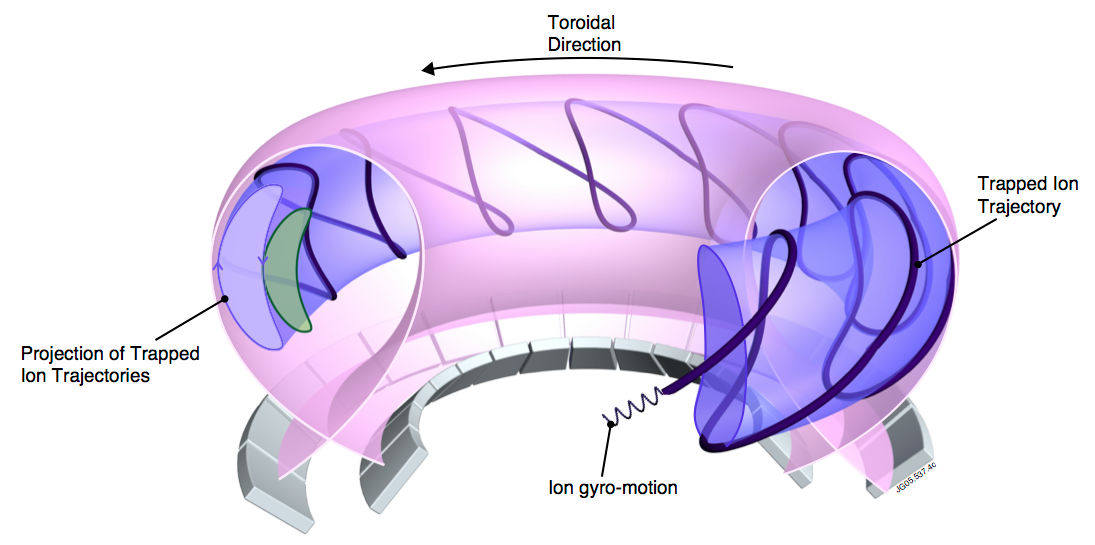
\includegraphics[height=6cm]{silocary_tok.png}
      \caption{Tokamak magnetic geometry and representative trapped-ion trajectories \cite{mlynar}.}
      \label{fig:silocary_tok}
\end{figure}

Unlike stellarators, where the magnetic configuration is determined almost entirely by the geometry of external coils, the engineering design of a tokamak is largely focused on maintaining precise control of the plasma current and plasma position.
The plasma cross-section is intentionally elongated and triangular because these shaping parameters improve plasma stability and allow higher plasma pressure before magnetohydrodynamic (MHD) instabilities occur.
The principal design variables are therefore the major radius $R$, minor radius $a$, plasma current $I_p$, toroidal magnetic field $B_t$, elongation $\kappa$ and triangularity $\delta$. These six parameters determine the overall performance of the device and are optimized according to the intended operating regime.
The axisymmetric configuration significantly simplifies both manufacturing and maintenance compared to stellarators.
\\
\\
Toroidal field coils are identical and can be manufactured repeatedly with relatively tight tolerances, while the vacuum vessel also follows a rotationally symmetric geometry.
This simplicity was one of the main reasons why tokamaks became the dominant concept in magnetic confinement research throughout the second half of the twentieth century.
Experimental facilities such as JET demonstrated reactor-relevant plasma performance, and the same design philosophy has been adopted for ITER and the European DEMO reactor.
\\
\\
Despite these advantages, tokamaks require sophisticated active control systems to maintain plasma equilibrium throughout the discharge.
Feedback control of plasma current, vertical stability, and plasma position is essential for safe operation, particularly in large, high-performance devices.
Consequently, advances in diagnostics, control algorithms, and power electronics have become an integral part of modern tokamak engineering.

\pagebreak
\subsection{Magnetic confinement - Stellarator design}
Conditions for nuclear fusion in the Sun are created by the gravitational forces of the Sun's mass. 
One of the engineering solutions to achieve the same conditions is magnetic confinement.
Positively charged atomic nuclei are held by a magnetic field on a very close distance to allow the fusion reaction.
Tokamak and stellarator are two leading designs of fusion reactor with the magnetic confinement.
Both designs were developed in the 1950's, tokamak design originates in the USSR Kurchatov Institute, the first stellarator was constructed and operated on Princeton university (USA).
The first stellarator with a figure 8 shape was proposed in 1958 by Lyman Spitzer as a part of "Project Matterhorn", shown in Figure \ref{fig:prvni_stell}.
\\
\vspace{-0.5cm}
\begin{figure}[h]
  \centering
  \begin{minipage}{0.35\textwidth}
      \centering
      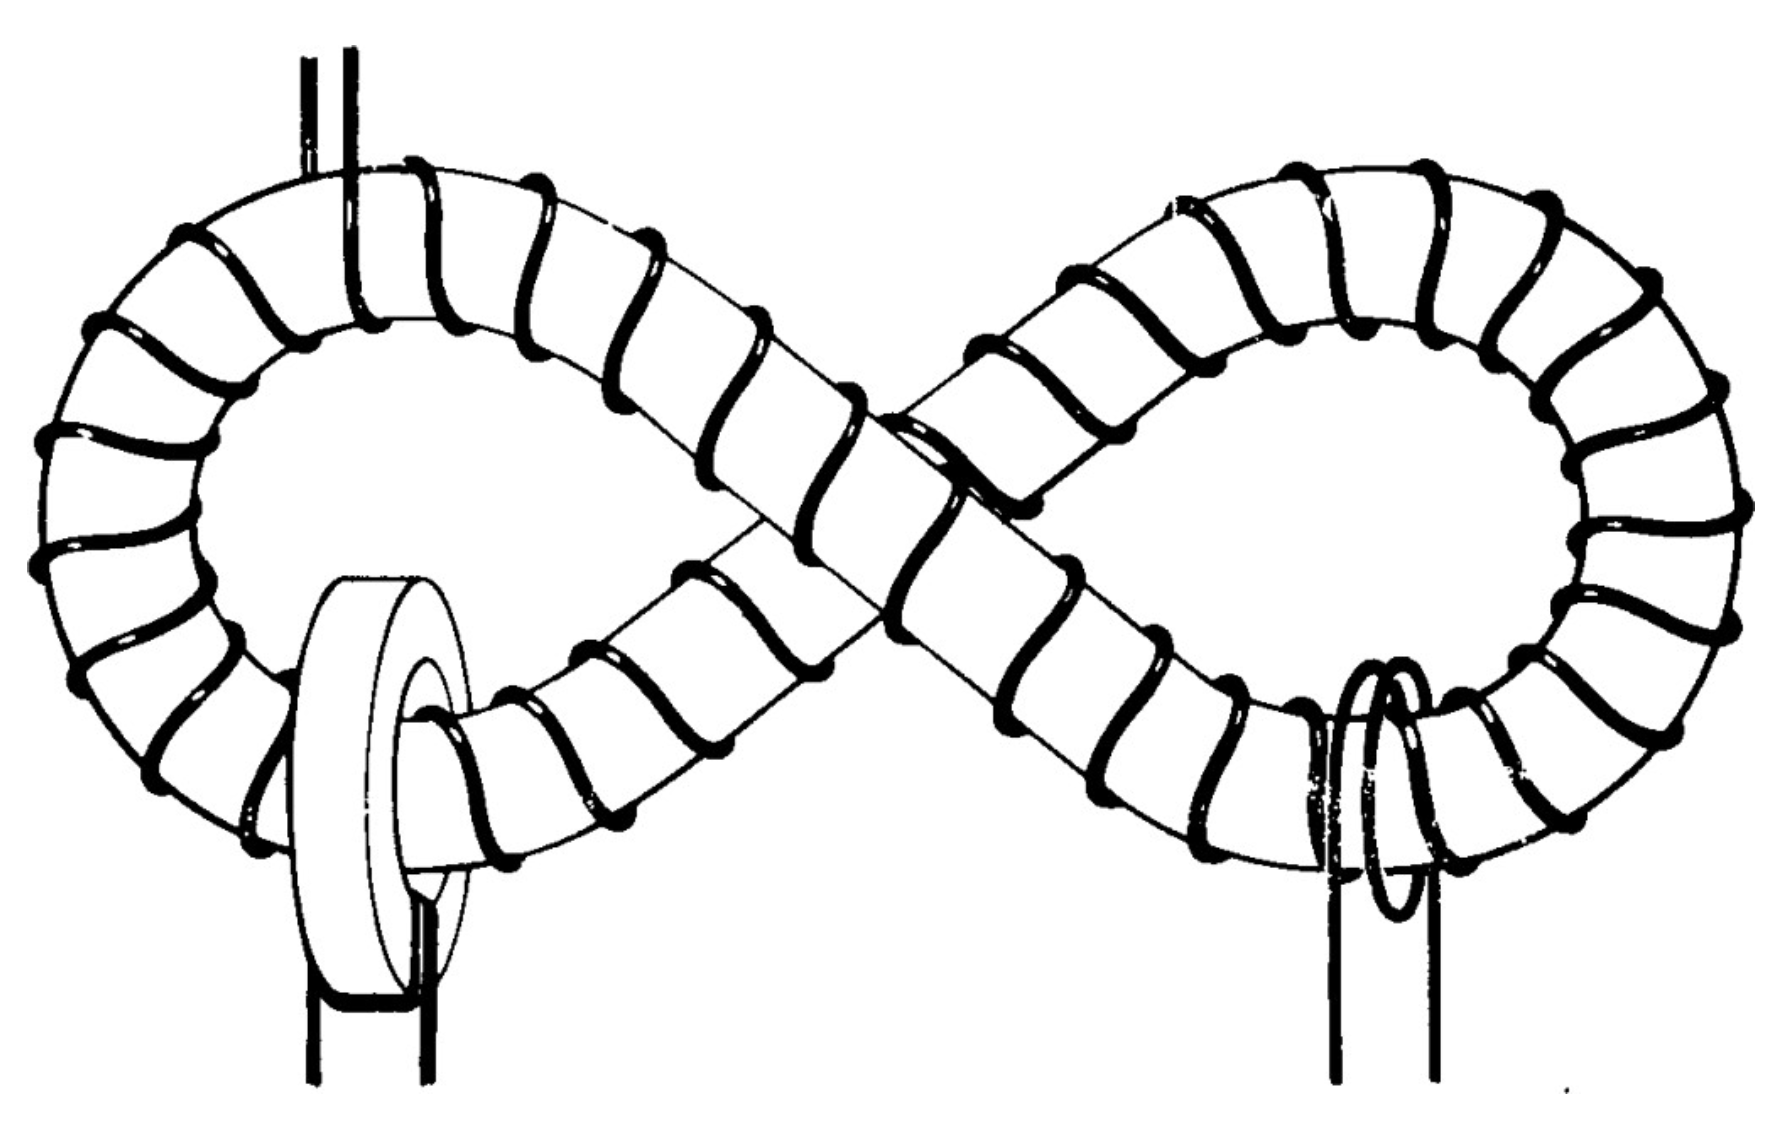
\includegraphics[width=\linewidth]{prvni_stelarator.png}
      \caption{The first stellarator \\ design "Project Matterhorn"\cite{spitzer_paw_2024}}
      \label{fig:prvni_stell}
  \end{minipage}\hfill
  \begin{minipage}{0.60\textwidth}
      \centering
      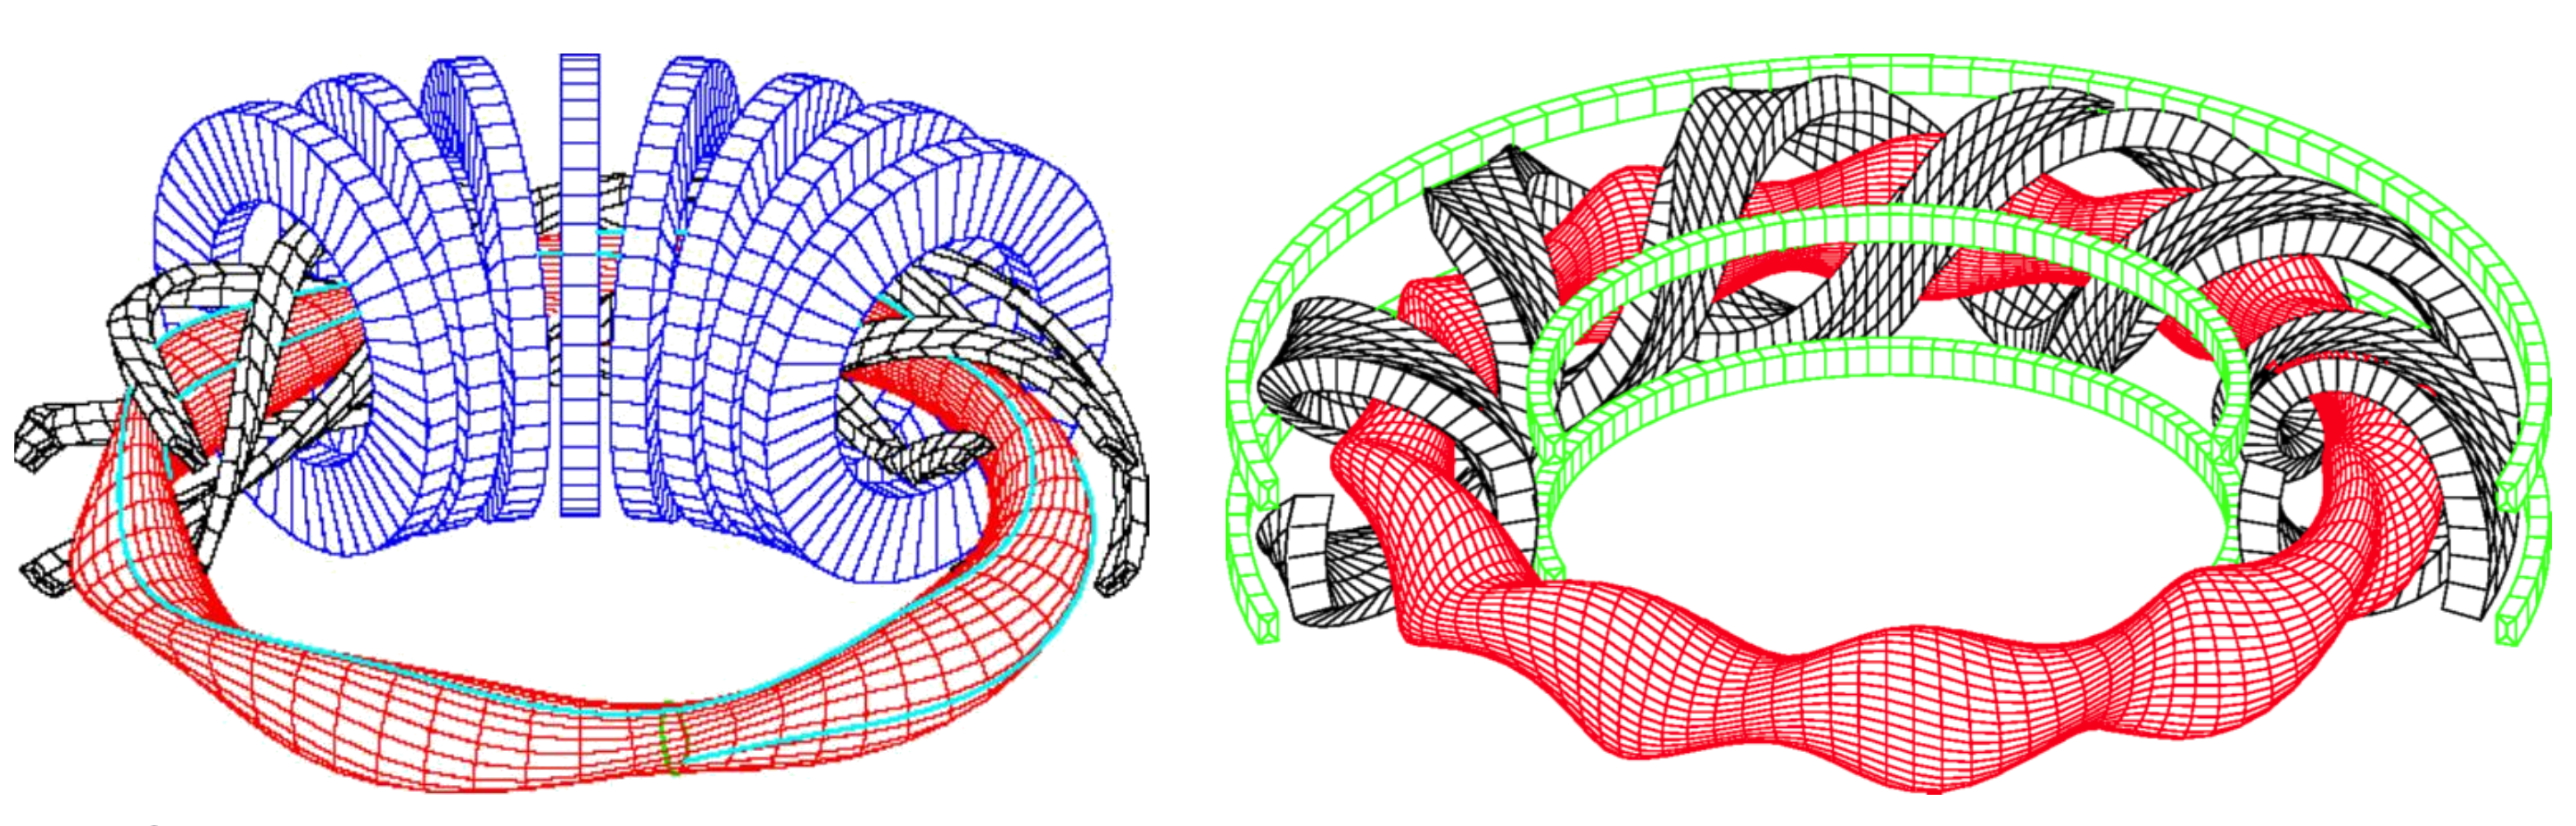
\includegraphics[width=\linewidth]{stellaratory_dva.png}
      \caption{Classical stellarator (left): helical currents anti-parallel, requires toroidal field coils and Torsatron/Heliotron (right): helical currents parallel, requires vertical field coils \cite{kniha_2018}.}
      \label{fig:dva_stell}
  \end{minipage}
\end{figure}

\noindent The required poloidal component of the magnetic field is generated by an inductive plasma current, this current is a very efficient mean of plasma heating, but creates many difficulties with steady state operation and current instabilities.
On the other side, all of the stellarator magnetic fields are generated by external coils. 
The crucial engineering difference is that a tokamak is axisymmetric in the toroidal direction, whereas stellarators rely on three-dimensional, non-axisymmetric magnetic fields and therefore require more complex coil geometries (Figure \ref{fig:dva_stell}).
One of the primary research challenge is to optimize the design of the magnetic fields to ensure good neoclassical plasma confinement.

\begin{equation}
  n T \tau_E \geq \mathrm{const.}  \; \; [m^{-3} \cdot s \cdot keV]
  \label{eq:lawson}
\end{equation}
where $n$ is the plasma particle density, $T$ is the plasma temperature and $\tau_E$ is the energy confinement time. The required value of the triple product depends on the fusion reaction and on the selected power-balance criterion.

\noindent In order to evaluate the Lawson criterion (Equation \ref{eq:lawson}) for stellarators, Equation \ref{eq:yamada} by Yamada is applied to predict the energy confinement $\tau_E$.
With a fixed value of $\iota_{2/3}$, the approximate scaling of the triple product can be expressed by Equation \ref{eq:tripple}.

\begin{equation}
  \tau_E^{\mathrm{ISS04}}=206 \cdot f_{ren} \cdot \mu_0^{-0.54} \cdot A^{-2.28} \cdot R_0^{2.92} \cdot P_h^{-0.61} \cdot \beta^{0.54} \cdot T^{-0.54} \cdot B^{1.92} \cdot \iota_{2/3}^{0.41}
  \label{eq:yamada}
\end{equation}
In Equation \ref{eq:yamada}, $f_{\mathrm{ren}}$ is the renormalization factor of the ISS04 scaling, $\mu_0$ is the vacuum permeability, $A$ is the aspect ratio, $R_0$ is the major radius, $P_h$ is the heating power, $\beta$ is the ratio of plasma pressure to magnetic pressure, $T$ is the plasma temperature, $B$ is the magnetic-field strength and $\iota_{2/3}$ is the rotational transform evaluated at the normalized radius $2/3$.

\noindent Equation \ref{eq:tripple} shows the triple product increasing with magnetic field strength ($B$) and plasma volume ($V_p$).
The volume of plasma ($V_p$) can be related by major radius ($R_0$) and aspect ratio ($A$). 
Aspect ratios are usually much larger in stellarators, compared to the tokamaks. 
An overview of aspect ratios and volumes of plasma in few selected fusion devices is shown in Table \ref{table:aspect_ratio}.

\begin{equation}
  n T \tau_E \propto  B^4 V_p T \; \; \; \; \; \; \; \; \; \;  V_p \propto  \dfrac{R^3}{A^2}
  \label{eq:tripple}
\end{equation}


\begin{center}
  \begin{table}[ht!]
    \centering
  \begin{tabular}{|l|c|c|c|c|}
  \hline
   & JET & LHD & W7-X & ITER \\
  \hline
  Major radius $R_0$ & 2.96 m & 3.9 m & 5.5 m & 6.2 m \\
  \hline
  Aspect ratio $A$ & \textbf{2.7} & \textbf{6.5} & \textbf{10.7} & \textbf{3.1} \\
  \hline
  Plasma volume $V_p$ & 100 $m^3$ & 30 $m^3$ & 30 $m^3$ & 900 $m^3$ \\
  \hline
  \end{tabular} 
  \caption{An overview of fusion device parameters.}
  \label{table:aspect_ratio}
\end{table}

\end{center}

\pagebreak

\noindent It is important to note the large helical coils shown in Figure \ref{fig:dva_stell} in both cases of the classical stellarator and Torsatron/Heliotron, those coils can be substituted by a set of modular coils.
Modular coils allow more flexibility and replaceability, a very crucial aspect considering the strict manufacturing and assembly tolerances of coils and the strong forces occurring during the operation.
Figures \ref{fig:imagestell1} and \ref{fig:imagestell2} show the basic geometrical dimensions of stellarator.
In a tokamak design, 6 degrees of freedom can be adjusted: major and minor radius, plasma current, toroidal field, elongation, triangularity.
In the case of a stellarator design, number of degrees of freedom is typically much larger (up to 100), providing much broader flexibility of the design.

\begin{figure}[h]
  \centering
  \hspace{-2cm}
  \begin{minipage}{0.5\textwidth}
      \centering
      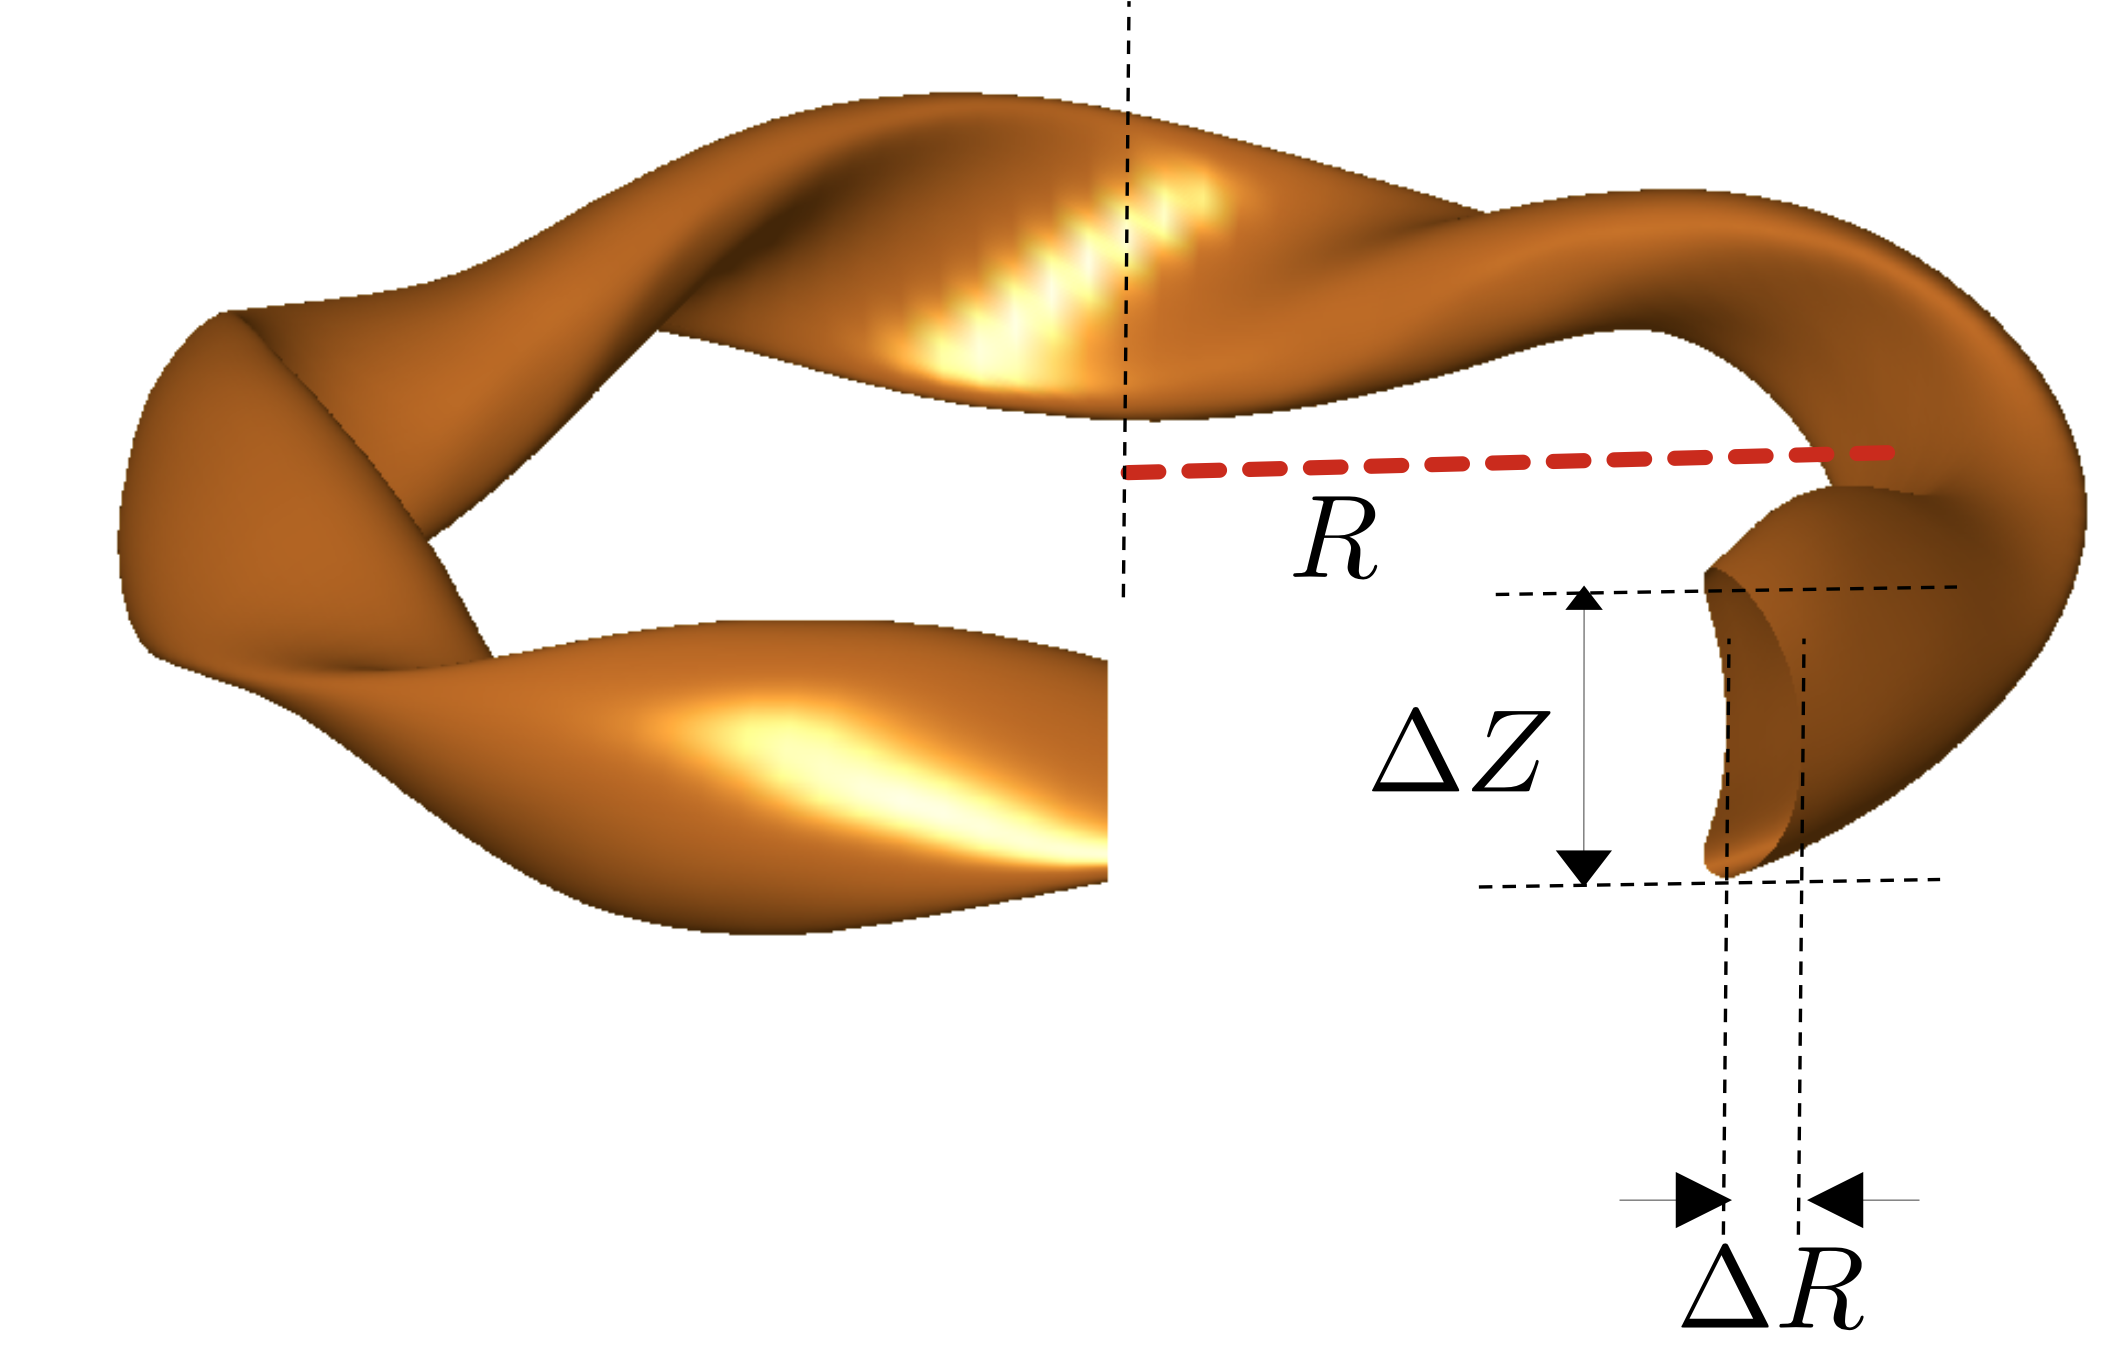
\includegraphics[height=0.5\linewidth]{stellarator_geometry_1.png}
      \caption{Plasma geometry \cite{Endler2021}.}
      \label{fig:imagestell1}
  \end{minipage}
  \hspace{0cm}
  \begin{minipage}{0.45\textwidth}
      \centering
      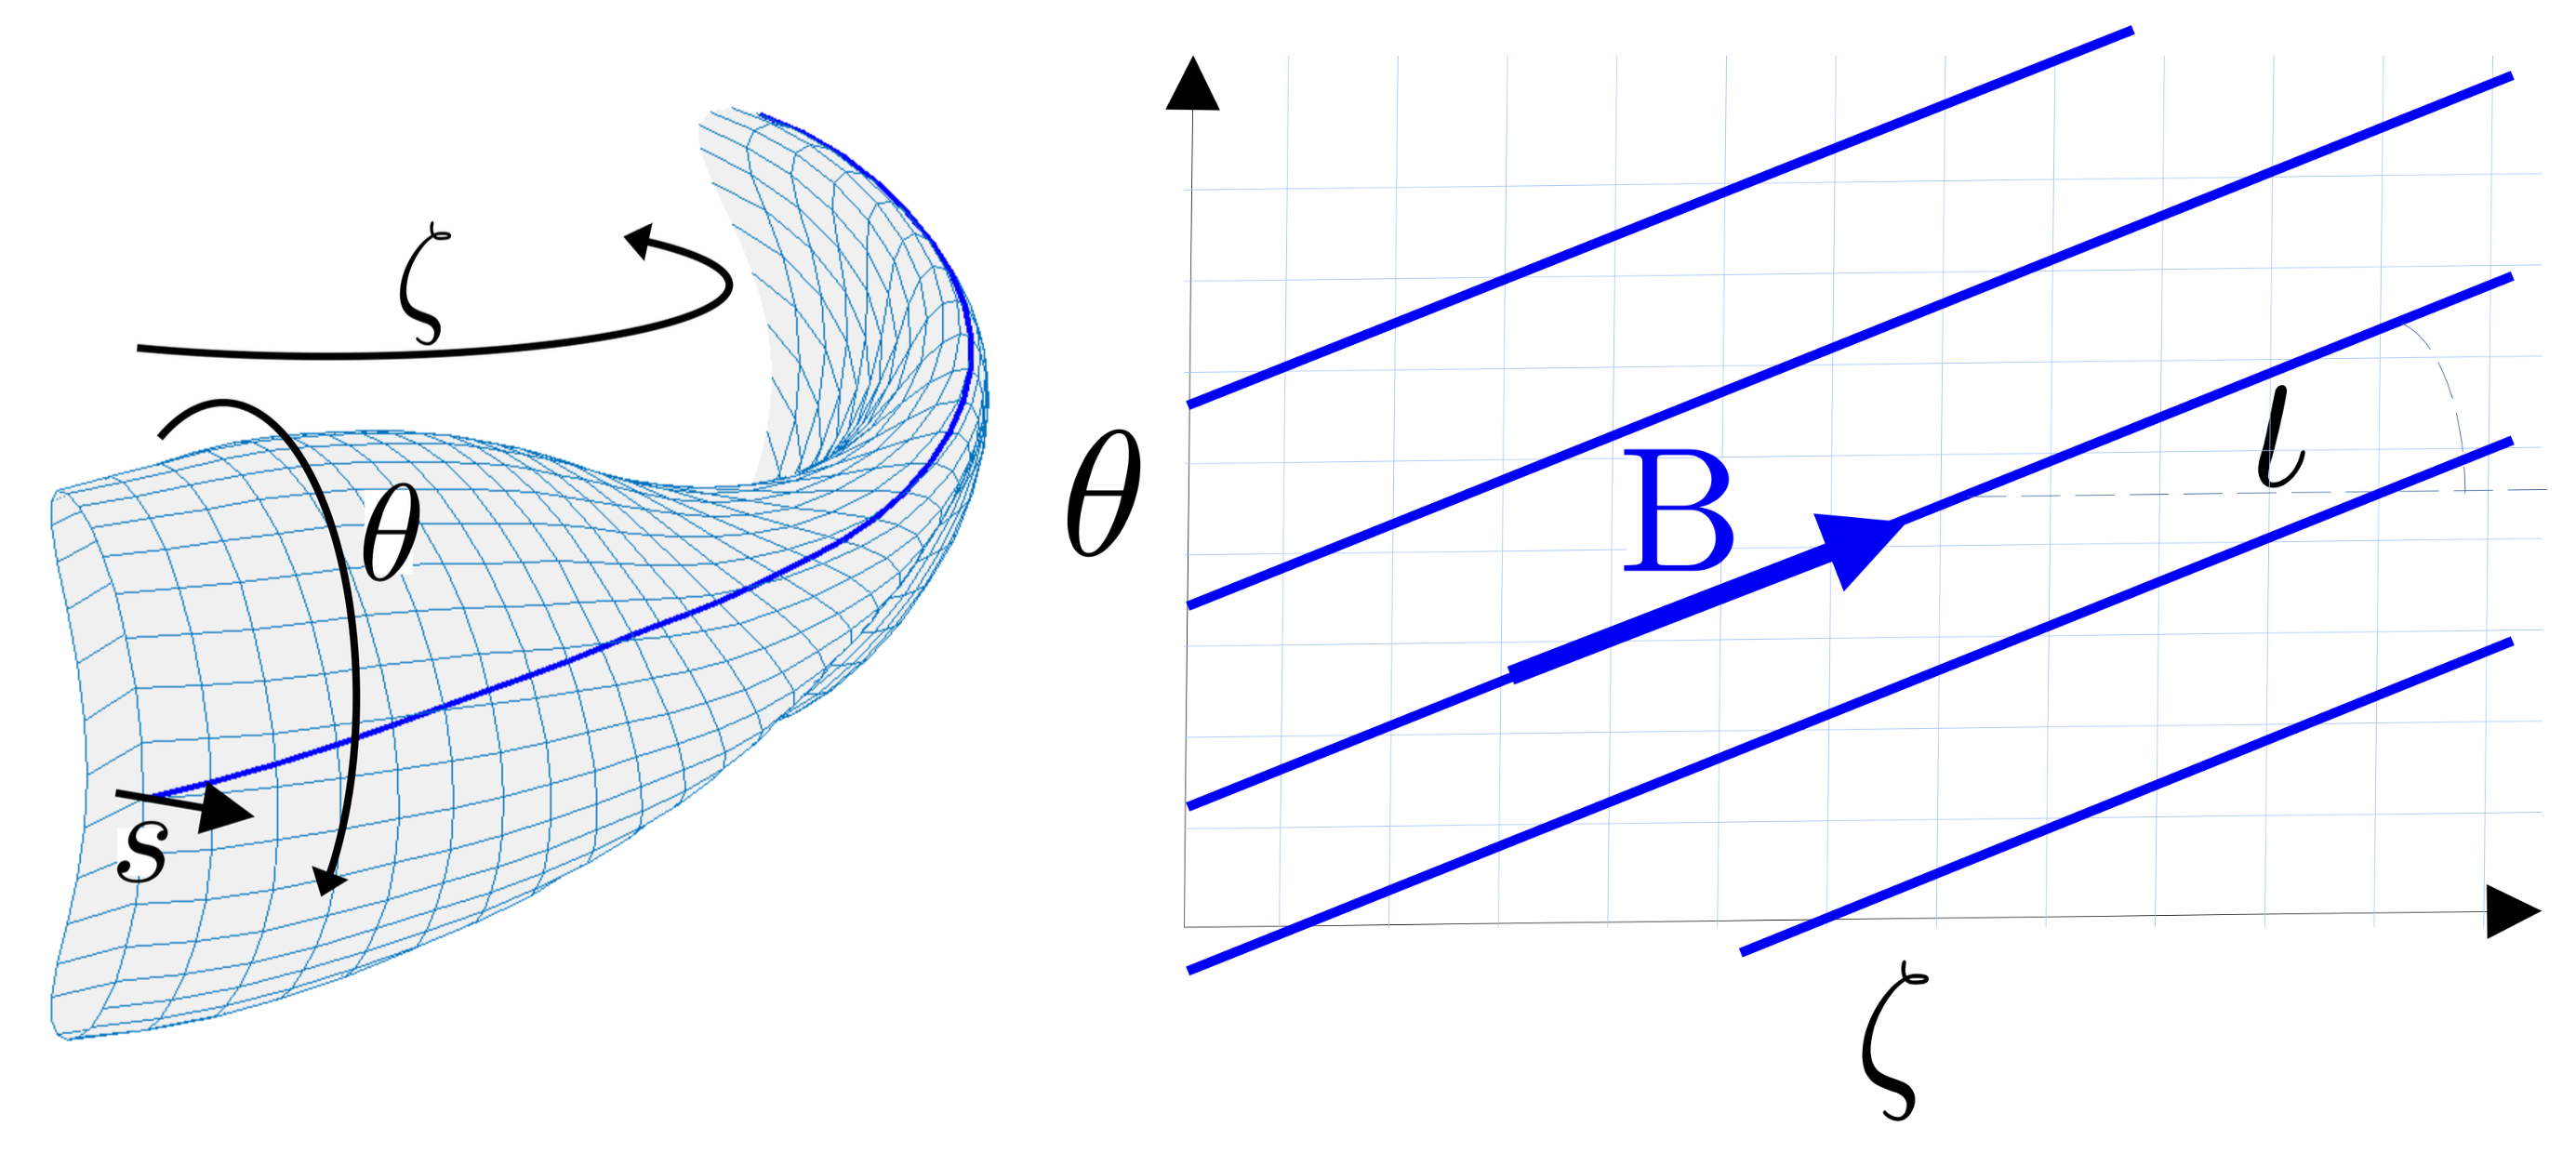
\includegraphics[height=0.5\linewidth]{magnetic_geom.png}
      \caption{Magnetic geometry coordinates \cite{Jorge2023}.}
      \label{fig:imagestell2}
  \end{minipage}
\end{figure}

\noindent Coordinates in the magnetic geometry are defined in three dimensions: toroidal $\zeta$, poloidal $\theta$ and radial $s$ (specifying the flux surface).
The elementary quantities are: major radius $R$, minor radius $a$, aspect ratio $A$, elongation $\kappa$, safety factor $q$ and the rotational transform $\iota$.

\begin{equation}
  a = \sqrt{\dfrac{V}{2 \cdot \pi^2 \cdot R}} \; \; \; \; \; \; \; \; \; \kappa=\dfrac{\Delta Z}{\Delta R} \; \; \; \; \; \; \; \; \; \iota = \dfrac{B \cdot \nabla \theta }{B \cdot \nabla \zeta}  \; \; \; \; \; \; \; \; \; q=\dfrac{2 \pi}{\iota}
\end{equation}

\noindent The rotational transform $\iota$ is very important parameter, defining the magnetic surface shape.
The rotational transform is used for both tokamaks and stellarators, although in a tokamak a substantial part of the poloidal field is generated by the plasma current, whereas in a stellarator the transform is produced predominantly by external coils.
If the rotational transform takes an irrational value, the magnetic field form a structure of nested magnetic surfaces, shown in Figure \ref{fig:ruzne_tvary_vrstev}: (a) for stellarator and (c) for tokamak.
If the rotational transform takes a rational value $\iota=\frac{i}{j}$, the field line closes over itself after $j$ toroidal turns and forms magnetic islands, shown in Figure \ref{fig:ruzne_tvary_vrstev}: (b) and (d).
The magnetic islands are not wanted in the plasma core, but can be beneficial in the region near the plasma edge.
The magnetic island can take a divertor function, to control the particle and heat exhaust, this concept was tested during operation of Wendelstein 7-AS and is now examined in the operation of Wendelstein 7-X.

\begin{figure}[h]
  \centering
  \begin{minipage}{0.157\textwidth}
      \centering
      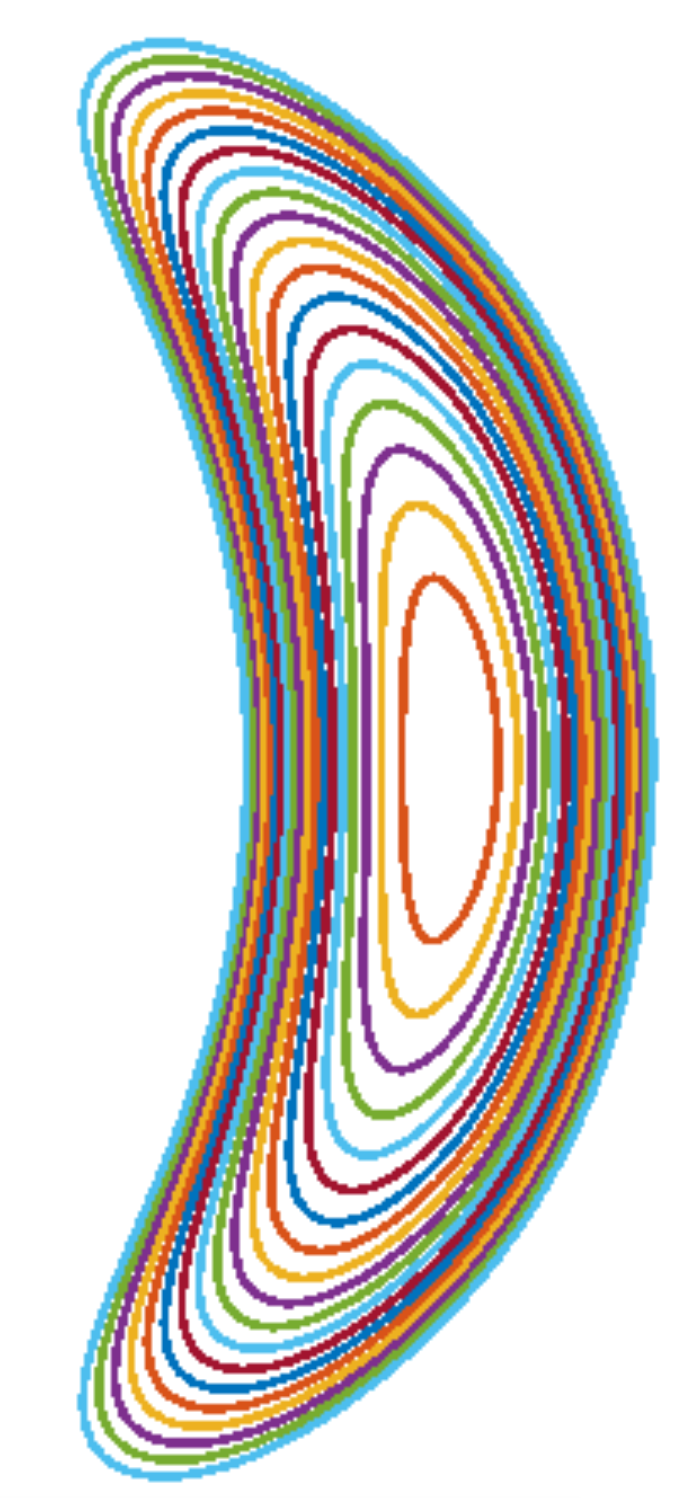
\includegraphics[width=\linewidth]{stell_cut_1.png}
      \caption*{a}
  \end{minipage}
  \begin{minipage}{0.18\textwidth}
      \centering
      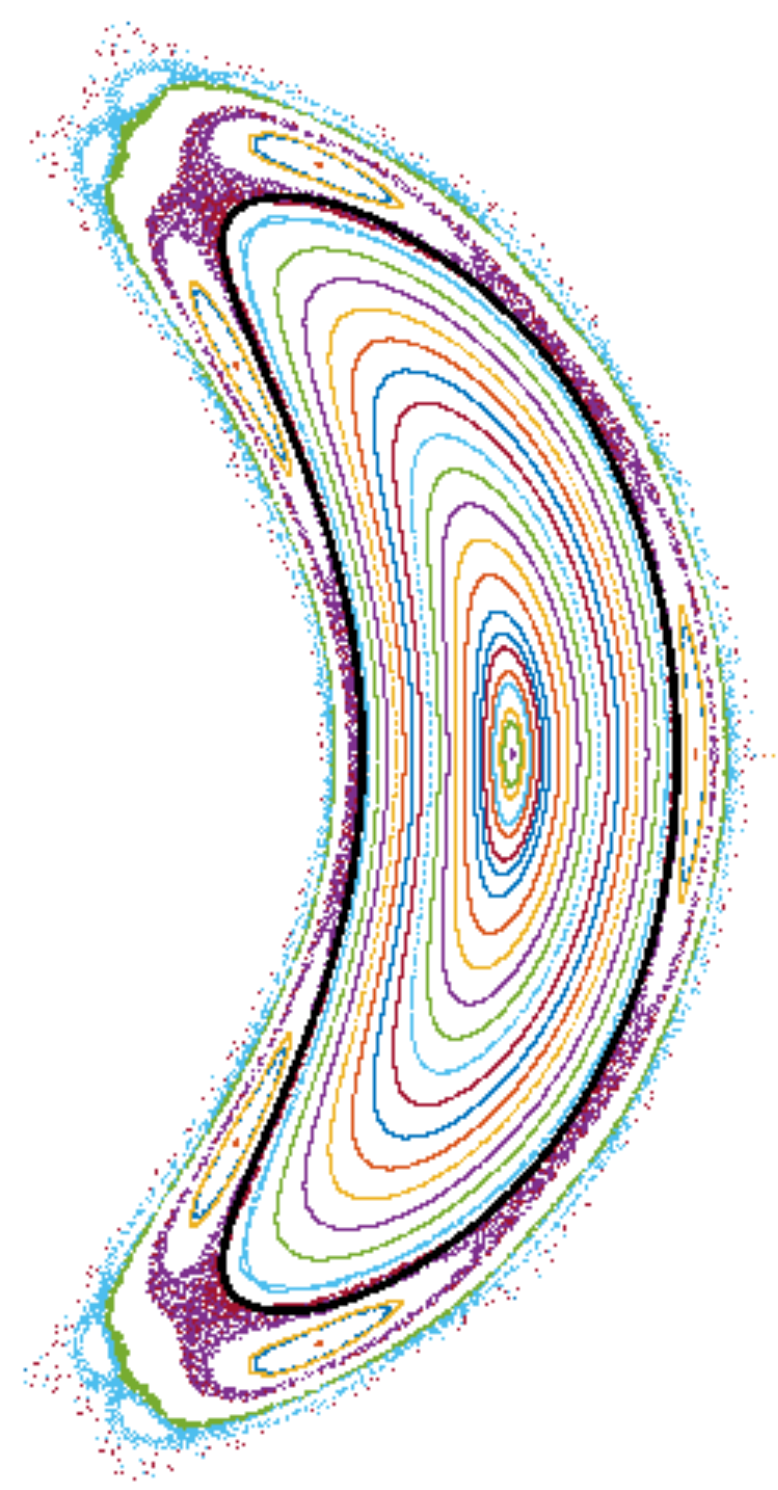
\includegraphics[width=\linewidth]{stell_cut_2.png}
      \caption*{b}
  \end{minipage}
  \begin{minipage}{0.27\textwidth}
    \centering
    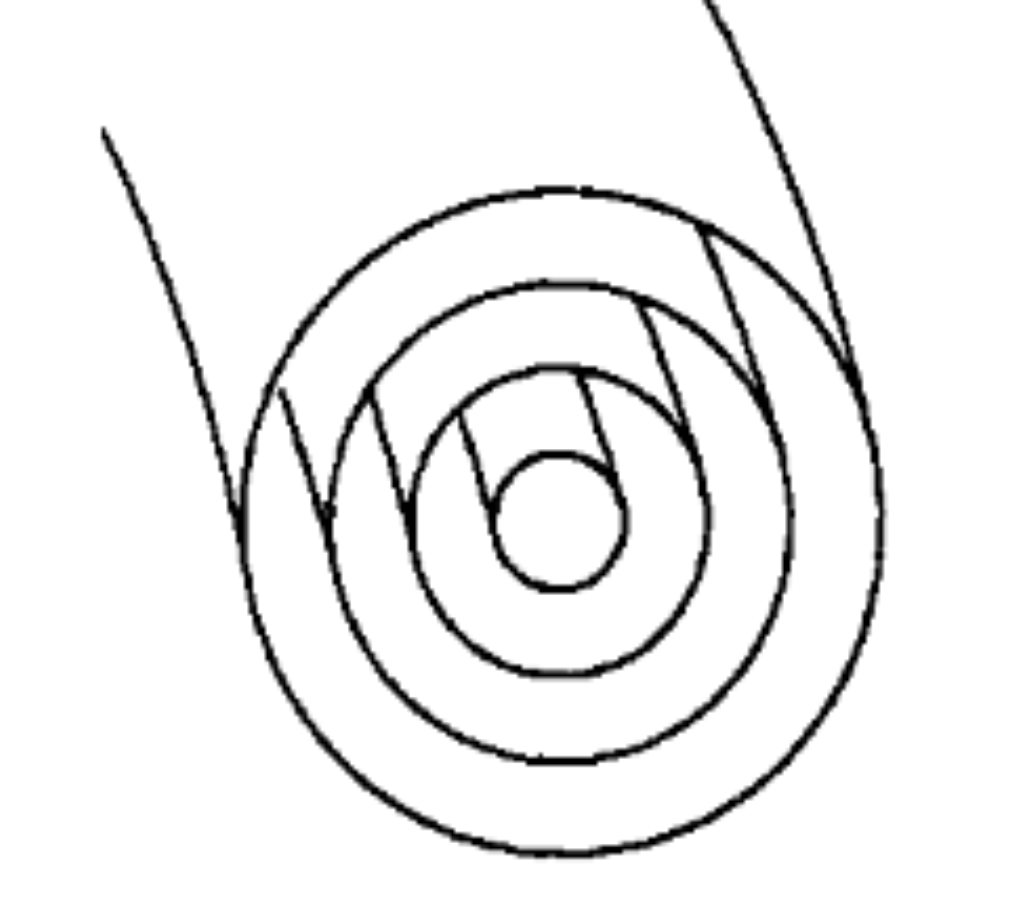
\includegraphics[width=\linewidth]{tokamak_cut_1.png}
    \caption*{c}
\end{minipage}
\begin{minipage}{0.27\textwidth}
  \centering
  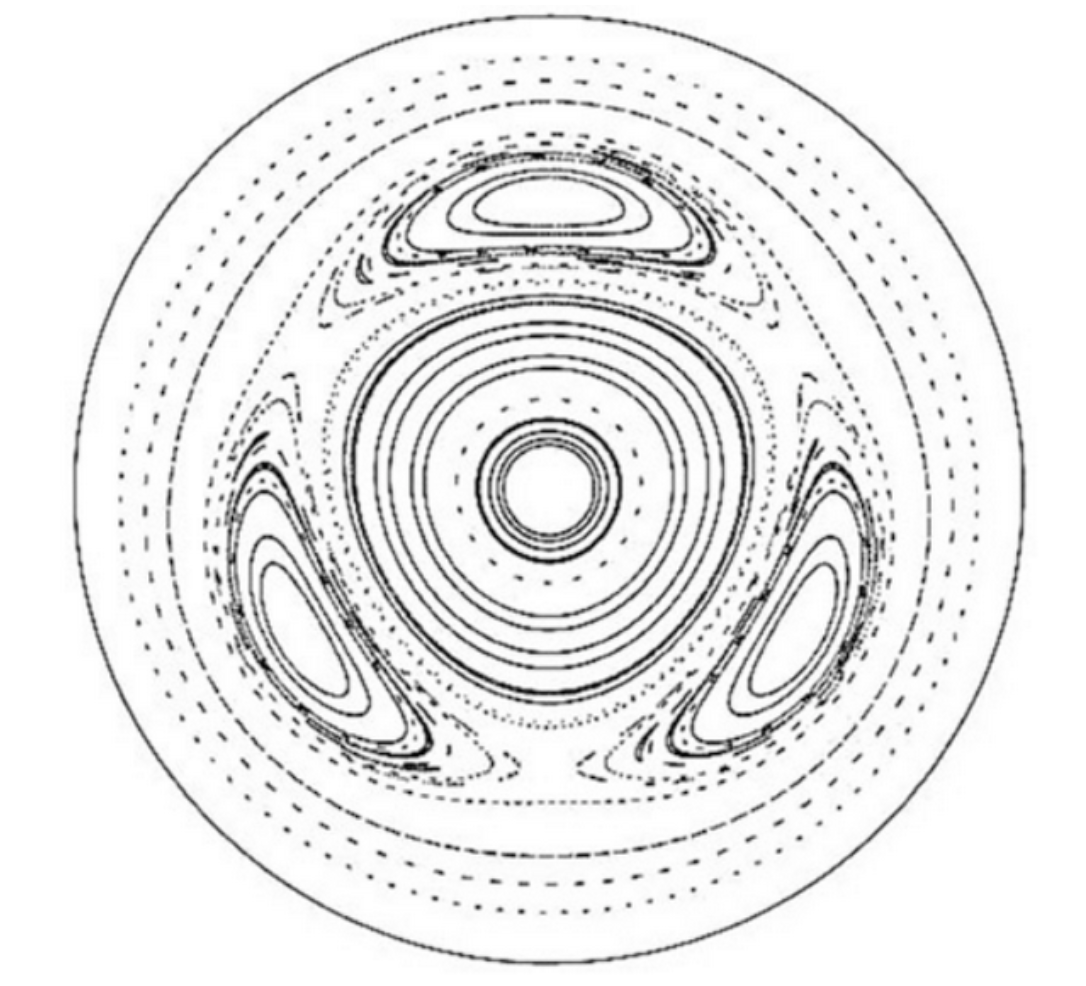
\includegraphics[width=\linewidth]{tokamak_cut_2.png}
  \caption*{d}
\end{minipage} 
\caption{Stellarator W7-X (a,b) and tokamak (c,d) magnetic surfaces \cite{Chen2011,Barton2015,Wang2020}.}
\label{fig:ruzne_tvary_vrstev}
\end{figure}


\pagebreak
\subsection{Public research}
The development of magnetic confinement fusion has been driven predominantly by publicly funded international research programs over the past several decades.
Experimental facilities have provided the scientific and engineering basis for future fusion power plants by investigating plasma confinement, plasma-facing materials, heating systems and power exhaust technologies.
Among these devices, tokamaks have achieved the highest plasma performance, while stellarators have recently attracted renewed interest due to their potential for steady-state operation.
The following sections present two representative examples of publicly funded fusion experiments: the Joint European Torus (JET), which established many of the operational scenarios adopted for ITER, and the Wendelstein 7-X stellarator, currently the world's largest superconducting stellarator and the leading experimental platform for optimized stellarator research.
\subsubsection{Tokamak: JET}
Joint European Torus (JET) was one of the most important experimental tokamaks in the history of nuclear fusion research. Together with the Tokamak Fusion Test Reactor (TFTR) in the United States, it formed the experimental basis for deuterium--tritium tokamak operation. The device was located at Culham Centre for Fusion Energy in the United Kingdom and operated as a joint European project. Its construction started in the 1970s and the first plasma was achieved in 1983. JET was designed as a large experimental facility capable of testing plasma scenarios relevant for future fusion reactors, especially with respect to deuterium-tritium operation, plasma heating, confinement and plasma-facing component behaviour.
\\
\\
The tokamak had a major radius of approximately 3 m and a minor radius of about 1 m. Due to its large plasma volume and strong magnetic field, JET was able to reach reactor-relevant plasma conditions. A crucial feature of JET was its ability to operate with deuterium-tritium fuel, which made it unique among fusion experiments for several decades. In 1997, JET achieved a fusion power of 16~MW, which represented a major milestone in magnetic confinement research. Later experimental campaigns focused on plasma scenarios directly supporting the ITER design, including operation with an ITER-like wall composed mainly of beryllium and tungsten.
\begin{figure}[h]
  \centering
      \centering
      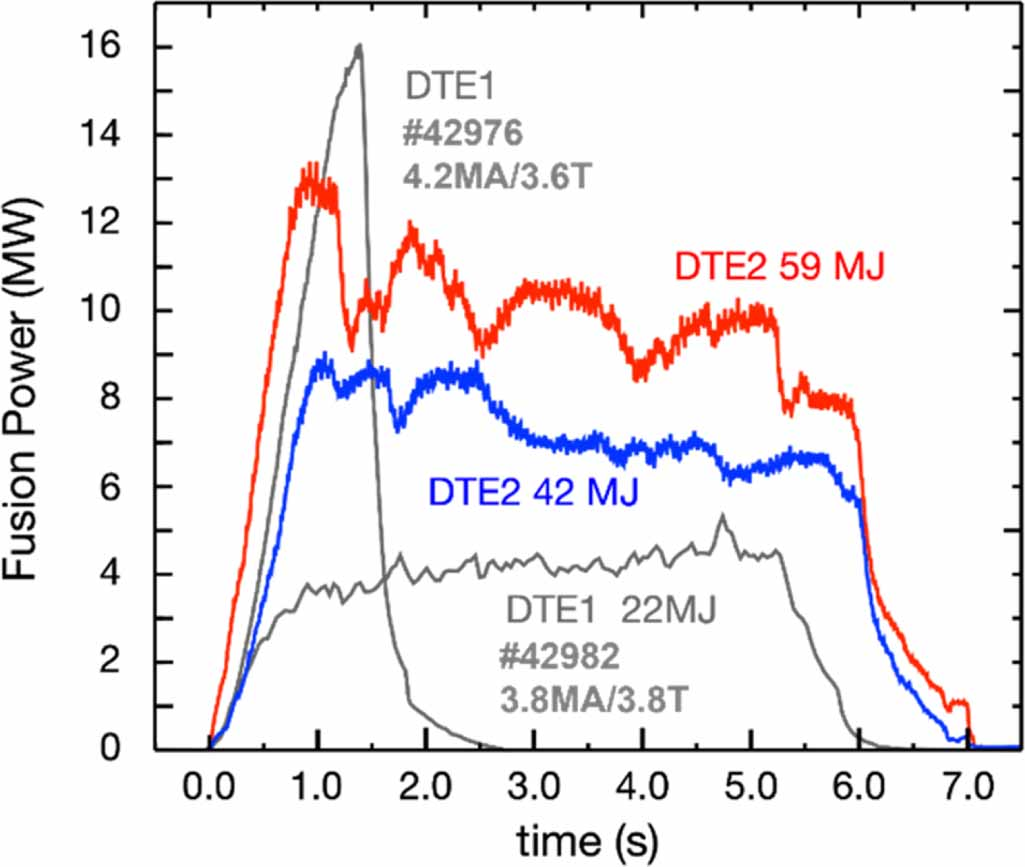
\includegraphics[height=9cm]{jet_record.jpg}
      \caption{Tokamak JET record of achieved fusion power \cite{jet_record}.}
      \label{fig:jet_record}
\end{figure}
\\
Figure \ref{fig:jet_record} compares selected deuterium-tritium plasma discharges performed during the first (DTE1) and second (DTE2) JET DT experimental campaigns. While the highest instantaneous fusion power of 16~MW was achieved during DTE1, the DTE2 campaign focused on sustaining fusion power over significantly longer pulse durations.
As a result, the total fusion energy produced increased from 22~MJ and 42~MJ in representative DTE1 discharges to a record value of 59~MJ during DTE2.
These results demonstrate the progress from achieving peak fusion performance towards stable, long-pulse operation, which is essential for the development of ITER and future fusion power plants.
From the engineering point of view, JET provided essential information about power exhaust, first wall loading and divertor operation. The installation of the ITER-like wall allowed researchers to study plasma-wall interaction with materials planned for ITER. This was particularly important because carbon-based plasma-facing materials, although favourable from the thermal point of view, are not suitable for future reactors due to tritium retention. The transition to metallic plasma-facing components therefore represented an important step towards reactor-relevant operation.
Figure \ref{fig:jet_obrazek} shows the JET tokamak schematic, including the vacuum vessel, toroidal field coils, poloidal field coils and the central solenoid.
\\
\\
JET also contributed significantly to the development of plasma heating and control systems. Neutral beam injection and radio-frequency heating were used to reach high plasma temperatures and to study advanced plasma regimes. The experience gained from JET operation influenced the design of ITER in many areas, including plasma scenarios, diagnostics, tritium handling and remote maintenance. After several decades of operation, JET was shut down in 2023, but its experimental results remain one of the key foundations for the next generation of tokamak fusion devices.
The final deuterium--tritium campaign (DTE3), performed in 2023, established a new JET fusion-energy record of 69~MJ released during a 6~s discharge \cite{EUROfusionDTE3}. The DTE3 result superseded the previous 59~MJ DTE2 record and provided a final validation dataset for ITER-relevant deuterium--tritium scenarios.
\\
\begin{figure}[h]
  \centering
      \centering
      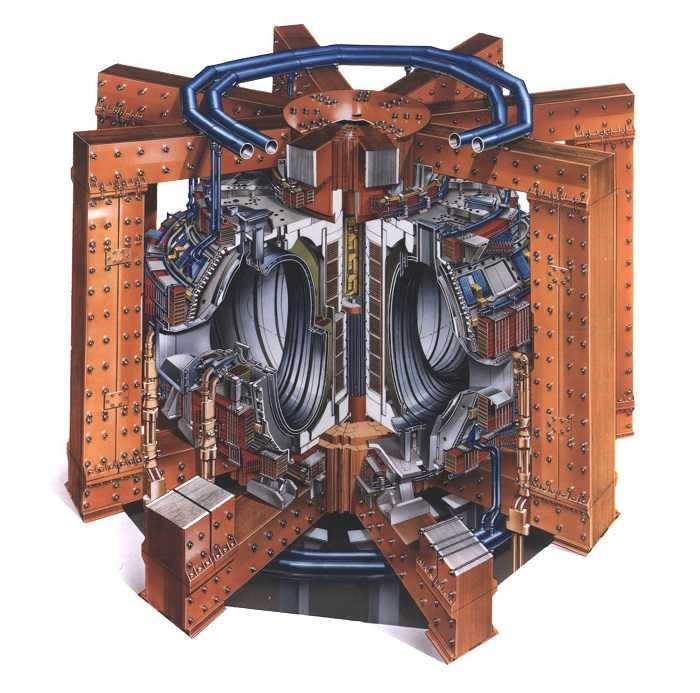
\includegraphics[height=9cm]{jet_obrazek.jpg}
      \caption{Tokamak JET schematic \cite{jet_obrazek}.}
      \label{fig:jet_obrazek}
\end{figure}
\pagebreak
\subsubsection{Stellarator: Wendelstein 7-X}
The Wendelstein stellarator line represents a pivotal series of devices in the development of nuclear fusion research. Named after the Wendelstein mountain in the Bavarian Alps, the stellarators built at the Max Planck Institute for Plasma Physics (IPP) have evolved significantly over the decades. Fusion research, declassified in 1958, was largely inspired by efforts like Project Matterhorn in the United States. The Wendelstein line began with modest devices but has since culminated in the world’s largest stellarator, the Wendelstein 7-X, which plays a critical role in advancing our understanding of controlled nuclear fusion.
The Wendelstein I devices marked the beginning of stellarator research in Germany. Wendelstein I-A was the first in the series, starting operations in 1960 with a major radius (R) of 35 cm, a minor radius (a) of approximately 2 cm, and a magnetic field strength (B) of up to 2 Tesla. The initial design was based on a racetrack configuration, which aimed to confine the plasma with an external magnetic field without relying on a plasma current.

\begin{figure}[h]
  \centering
  \begin{minipage}{0.42\textwidth}
      \centering
      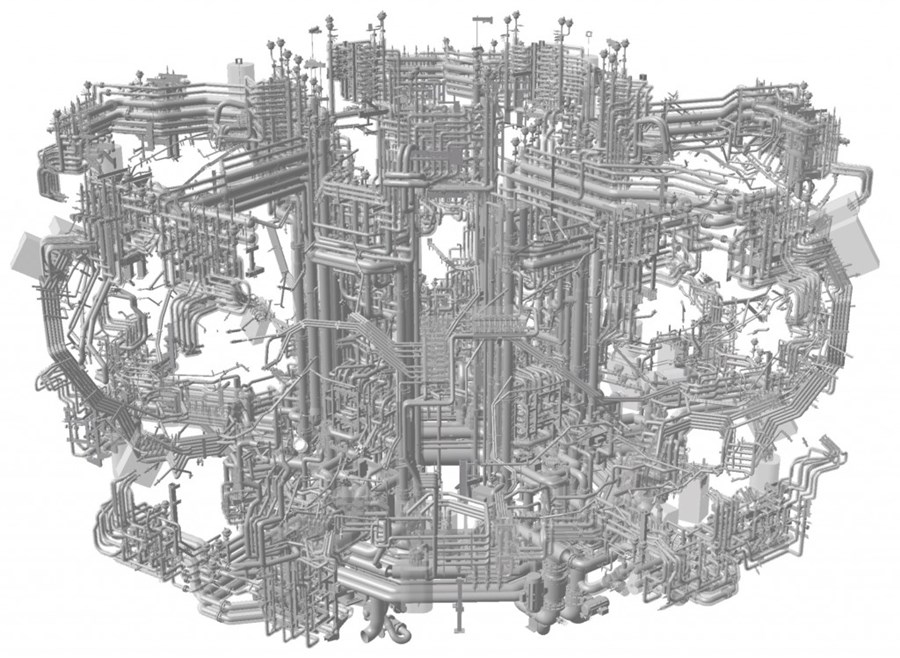
\includegraphics[height=3.7cm]{wend_2.png}
      \caption{W7-X's cooling piping \cite{iter2023stellarator}.}
      \label{fig:wend_1}
  \end{minipage}\hfill
  \begin{minipage}{0.55\textwidth}
      \centering
      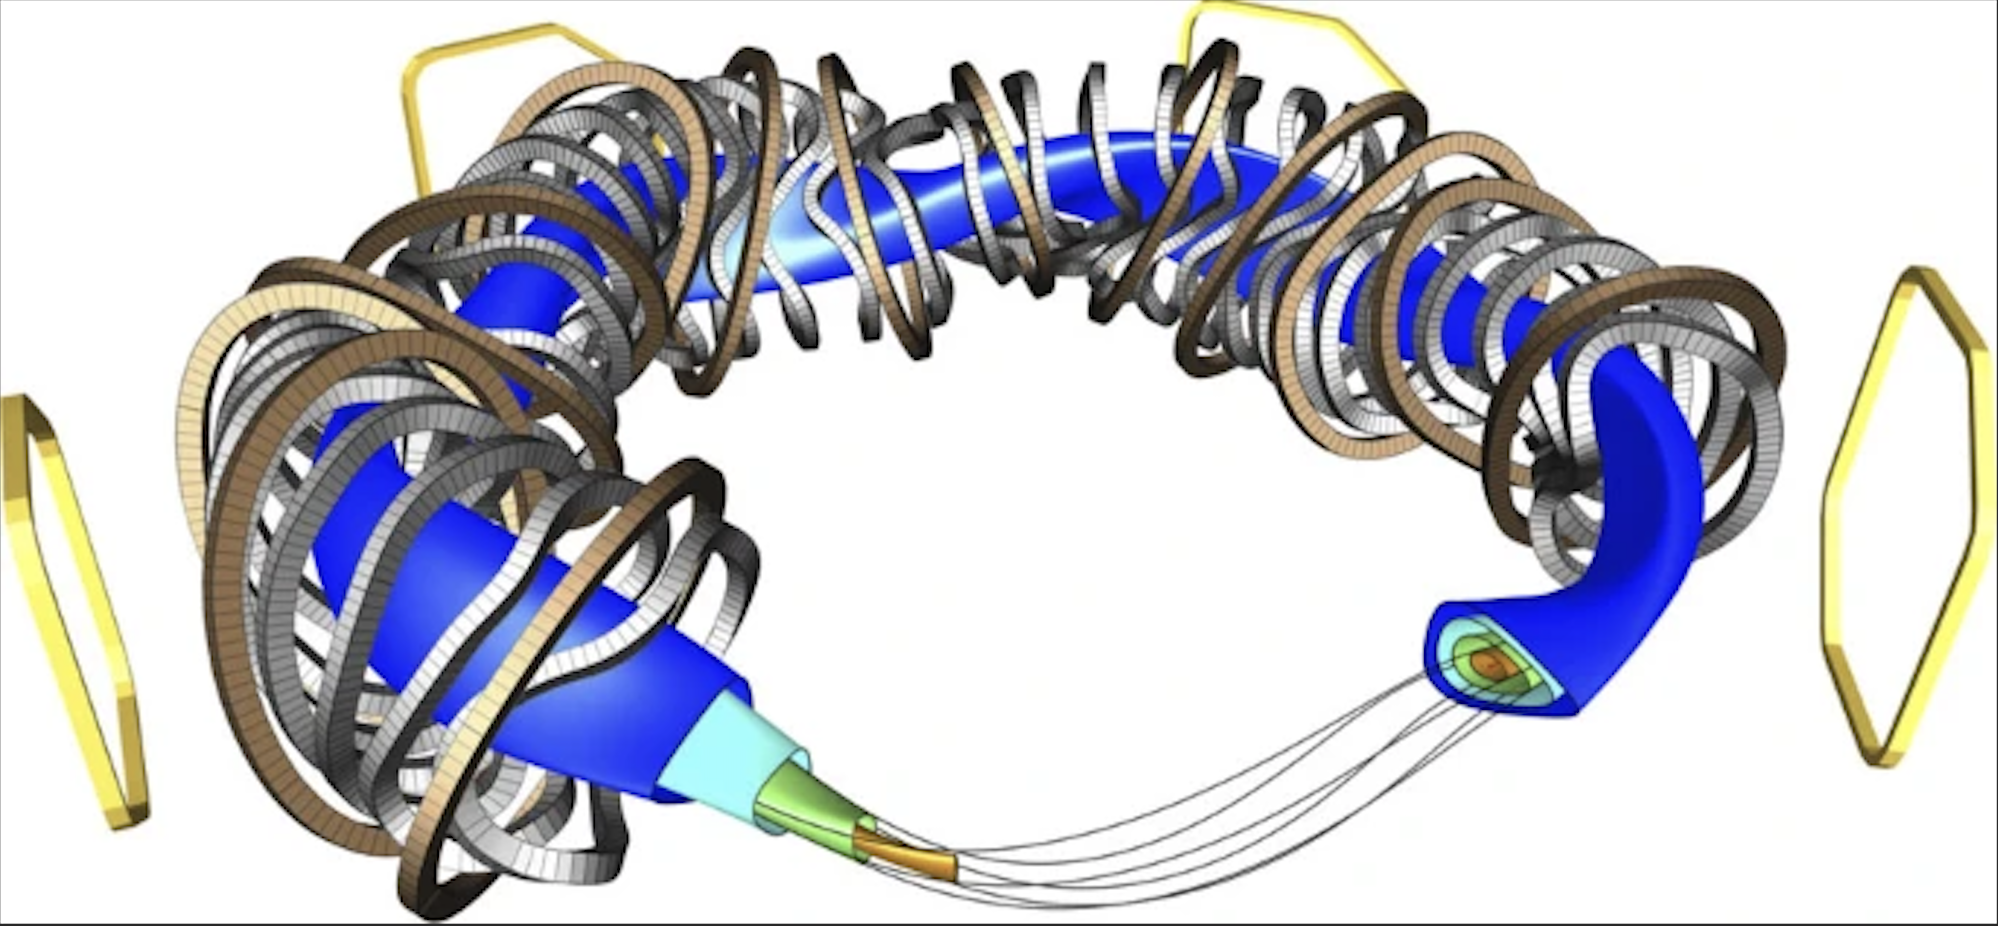
\includegraphics[trim={2mm 5mm 2mm 2mm},clip, height=3.7cm]{wcivky.png}
      \caption{W7-X magnetic coils and surfaces \cite{Pedersen2016}.}
      \label{fig:wend_2}
  \end{minipage}
\end{figure}
\noindent Wendelstein I-B was a slightly modified version of I-A, retaining the same physical dimensions but introducing a different twist in the magnetic configuration. These early experiments demonstrated good confinement of cesium plasmas, though results were highly sensitive to changes in the magnetic configuration. The researchers hypothesized that the racetrack design was limiting the device’s performance, leading to the decision to pursue a fully circular torus design in future iterations.
Wendelstein 7-A, operational from 1975 to 1985, was the first large-scale stellarator at IPP Garching. With a major radius of 2 meters and a minor radius of 12 cm, this device marked a significant leap forward in fusion research. Operating at magnetic field strengths up to 3.4 Tesla, Wendelstein 7-A was the first machine to demonstrate the confinement of plasma without the need for a plasma current—confirming the "pure" stellarator concept.
\\
\\
In 1988, Wendelstein 7-AS was introduced as an "Advanced Stellarator" at IPP. This machine, operational until 2002, had a major radius of 2 meters, a minor radius of approximately 0.2 meters, and magnetic fields up to 2.5 Tesla. Unlike its predecessors, Wendelstein 7-AS was the first large stellarator to incorporate modular coils. This design innovation allowed greater flexibility in shaping the magnetic fields, thereby improving plasma confinement and reducing Pfirsch-Schlüter currents, which are detrimental to confinement.
Wendelstein 7-AS achieved several notable milestones, including record plasma performance, with ion temperatures (Ti) reaching approximately 1.5 keV and electron temperatures (Te) around 6 keV. Furthermore, in 1992, it was the first stellarator to achieve high-confinement (H-mode) operation, which had previously been observed only in tokamaks. Another important innovation was the development of the island divertor concept, designed to control plasma impurities and heat loads on the reactor walls.
\begin{figure}[ht]
  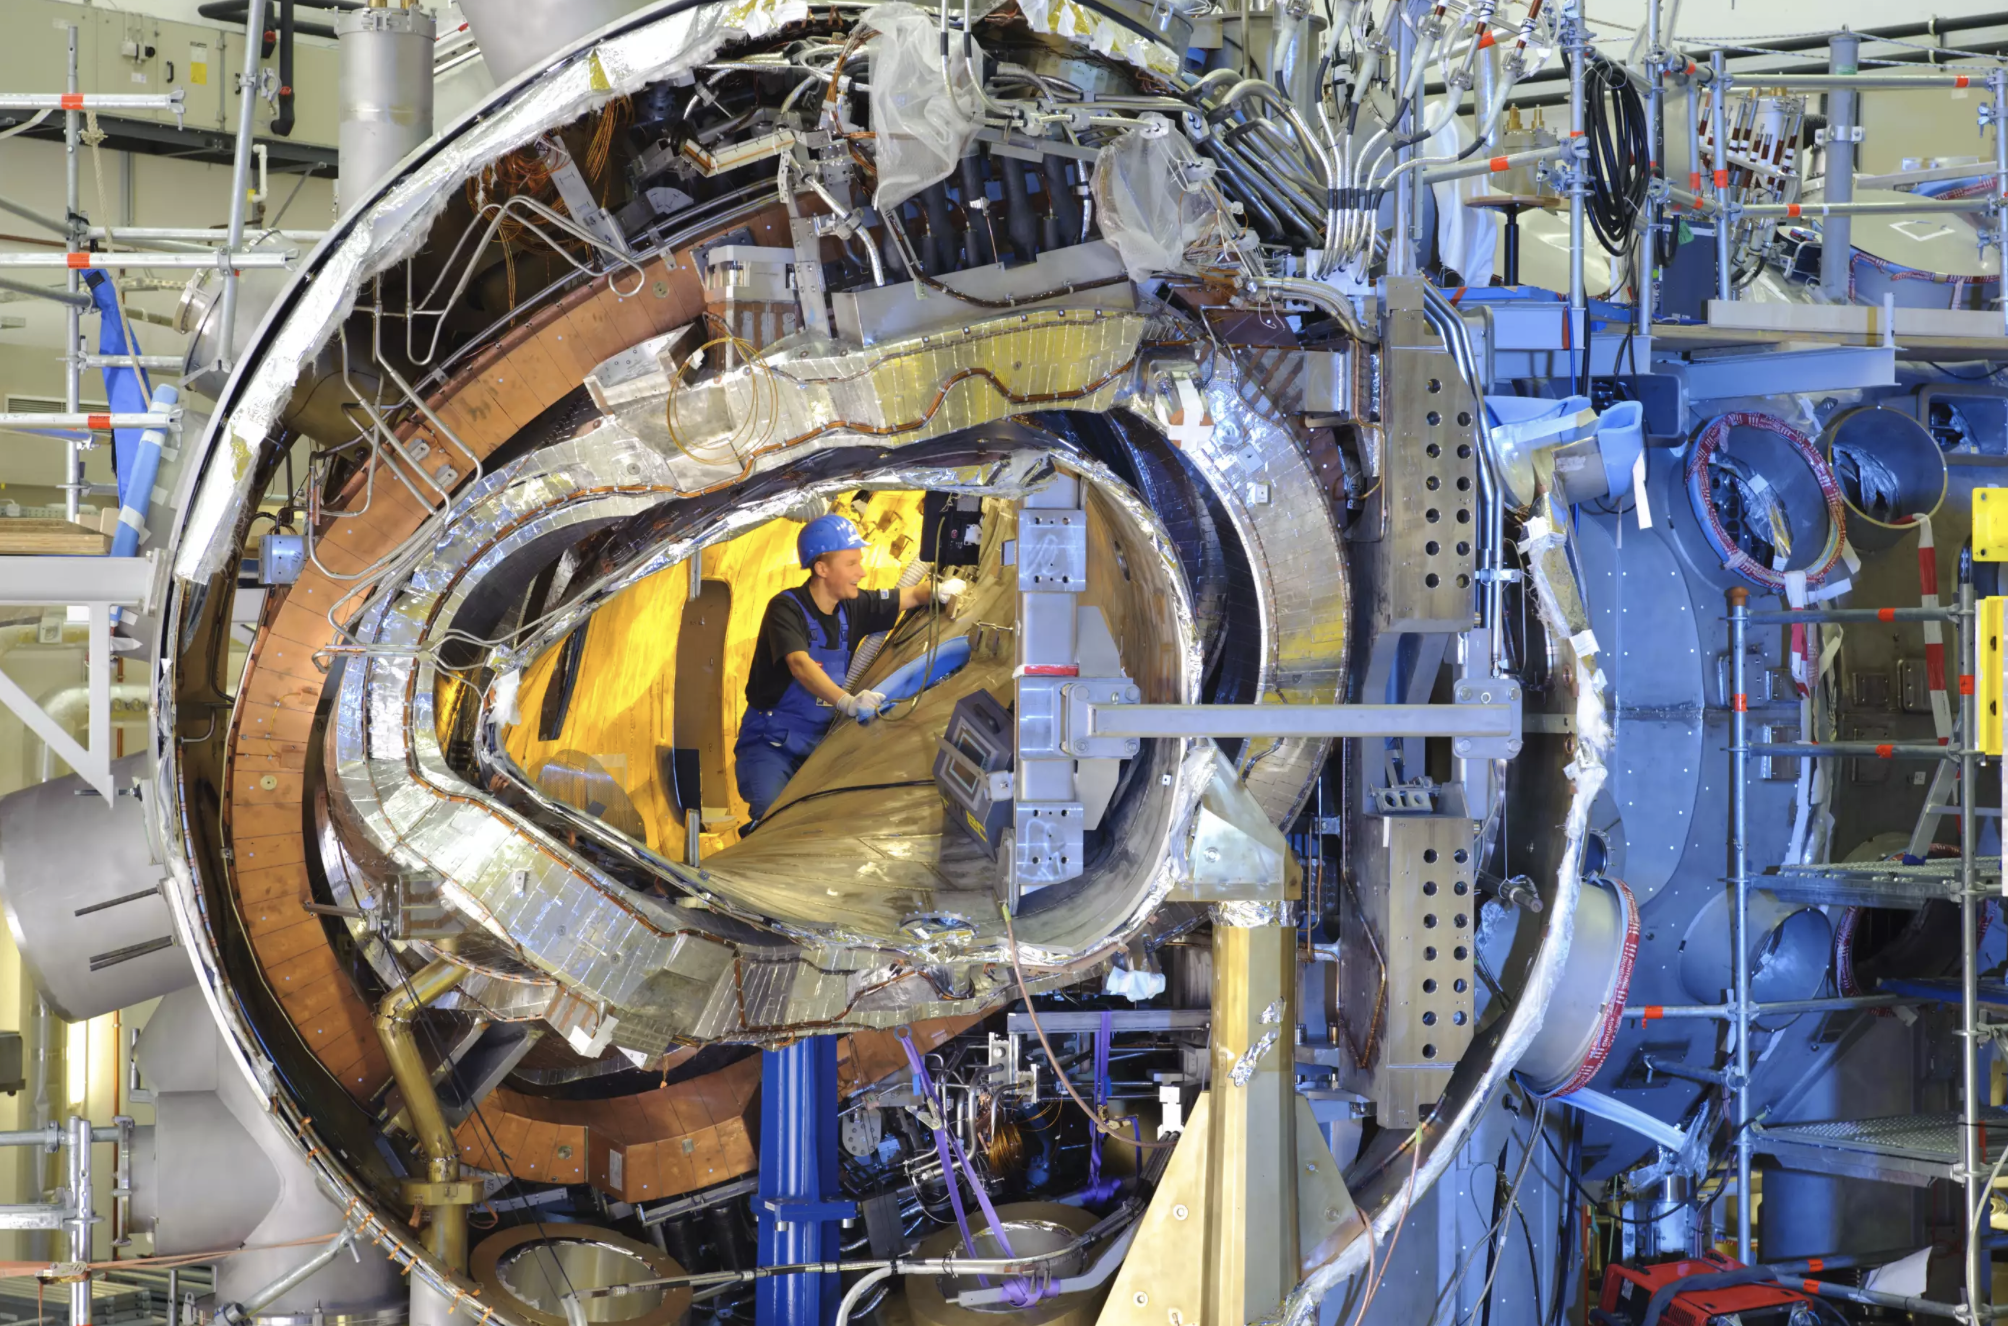
\includegraphics[width=10cm]{w7x_pohled.png}
  \centering
  \caption{In November 2011 it was still possible to look inside the Wendelstein 7-X: A worker is standing inside the bright yellow plasma vessel around which the solenoids are coiled. The photograph also shows the supporting structure and the outer vessel that encases the numerous cooling pipes and power supply lines \cite{maxplanck_wendelstein_2014}.}
  \label{fig:w7x_pohled}
\end{figure}
\noindent Wendelstein 7-X, located at IPP’s Greifswald branch, is the current flagship stellarator in the Wendelstein series and the largest of its kind in the world. Operational since 2015, the device has a major radius of 5.5 meters, an effective minor radius of 0.53 meters, and a magnetic field strength up to 3 Tesla.  Its design features 50 non-planar and 20 planar superconducting coils, which provide the necessary magnetic confinement for long-duration plasma experiments.

The fully water-cooled configuration has enabled W7-X to move from short-pulse commissioning towards reactor-relevant long-pulse operation. In the OP~2.3 campaign, completed in May 2025, W7-X sustained a record triple product for 43~s and increased the injected-energy turnover to 1.8~GJ during a 360~s plasma discharge \cite{IPPW7X2025}. These results are particularly relevant to high-heat-flux component development because sustained power exhaust, rather than short-duration peak performance alone, is a central requirement for a future stellarator power reactor.
The long-term programme remains directed towards high-performance plasma operation on the 30-minute timescale. A comparison of stellarator and tokamak operating regimes is shown in Figure \ref{fig:stell_tok}.
Healias is a design study for an upgraded five-periodic stellarator, performed at the Max Planck Institute for Plasma Physics as a successor of the Wendelstein evolutionary line \cite{Schauer2013}.
\begin{figure}[h]
  \centering
      \centering
      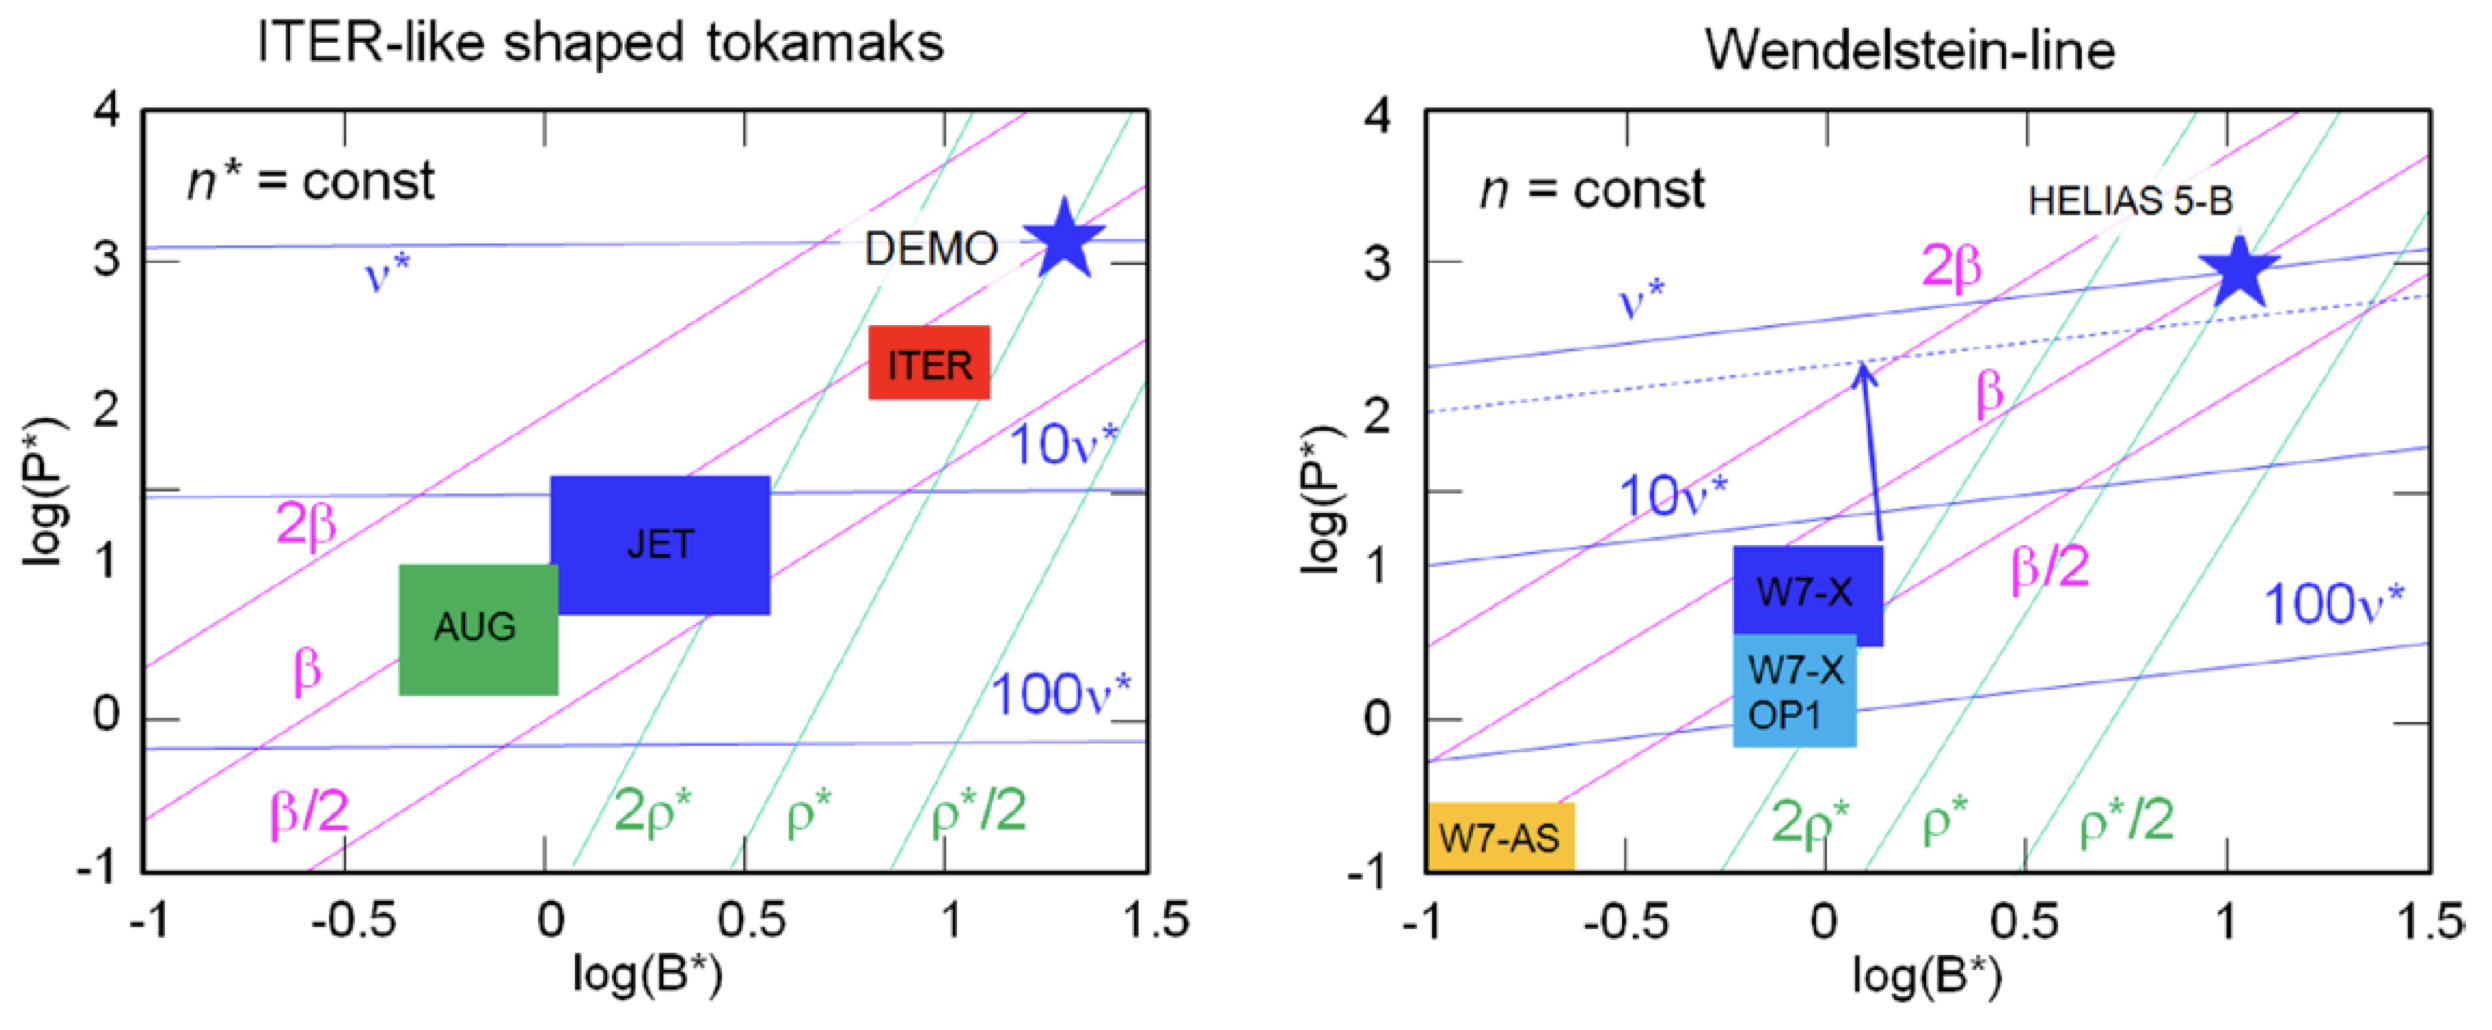
\includegraphics[height=5cm]{stell_tok.png}
      \caption{The left side shows operation windows of ASDEX Upgrade (AUG), JET and ITER in dimensionless engineering parameters with isocontours of dimensionless physics parameters at constant plasma density. The right side shows the same for the HELIAS line. The dotted line on the right side is the projection of the collisionallity of W7-X into the plane of HELIAS 5-B \cite{Warmer2016}.}
      \label{fig:stell_tok}
\end{figure}

\pagebreak
\subsubsection{Compass-U}
Research tokamak COMPASS-U is a new European fusion research facility under construction at the Institute of Plasma Physics of the Czech Academy of Sciences in Prague, Czech Republic.
It is a major upgrade of the previous COMPASS tokamak, which was operational from 2000 to 2016.
\\
\\
COMPASS-U will be a high magnetic field device with plasma geometries that are currently lacking in the European fusion program and globally, particularly after the shutdown of Alcator C-MOD. 
The goal of the project is to build a unique experimental device capable of supporting ITER operations and addressing key challenges in the design and construction of the DEMO reactor. 
The design and construction of the COMPASS-U tokamak involve broad participation from European and international partners, with operations expected to begin in 2030.



\begin{figure}[h]
  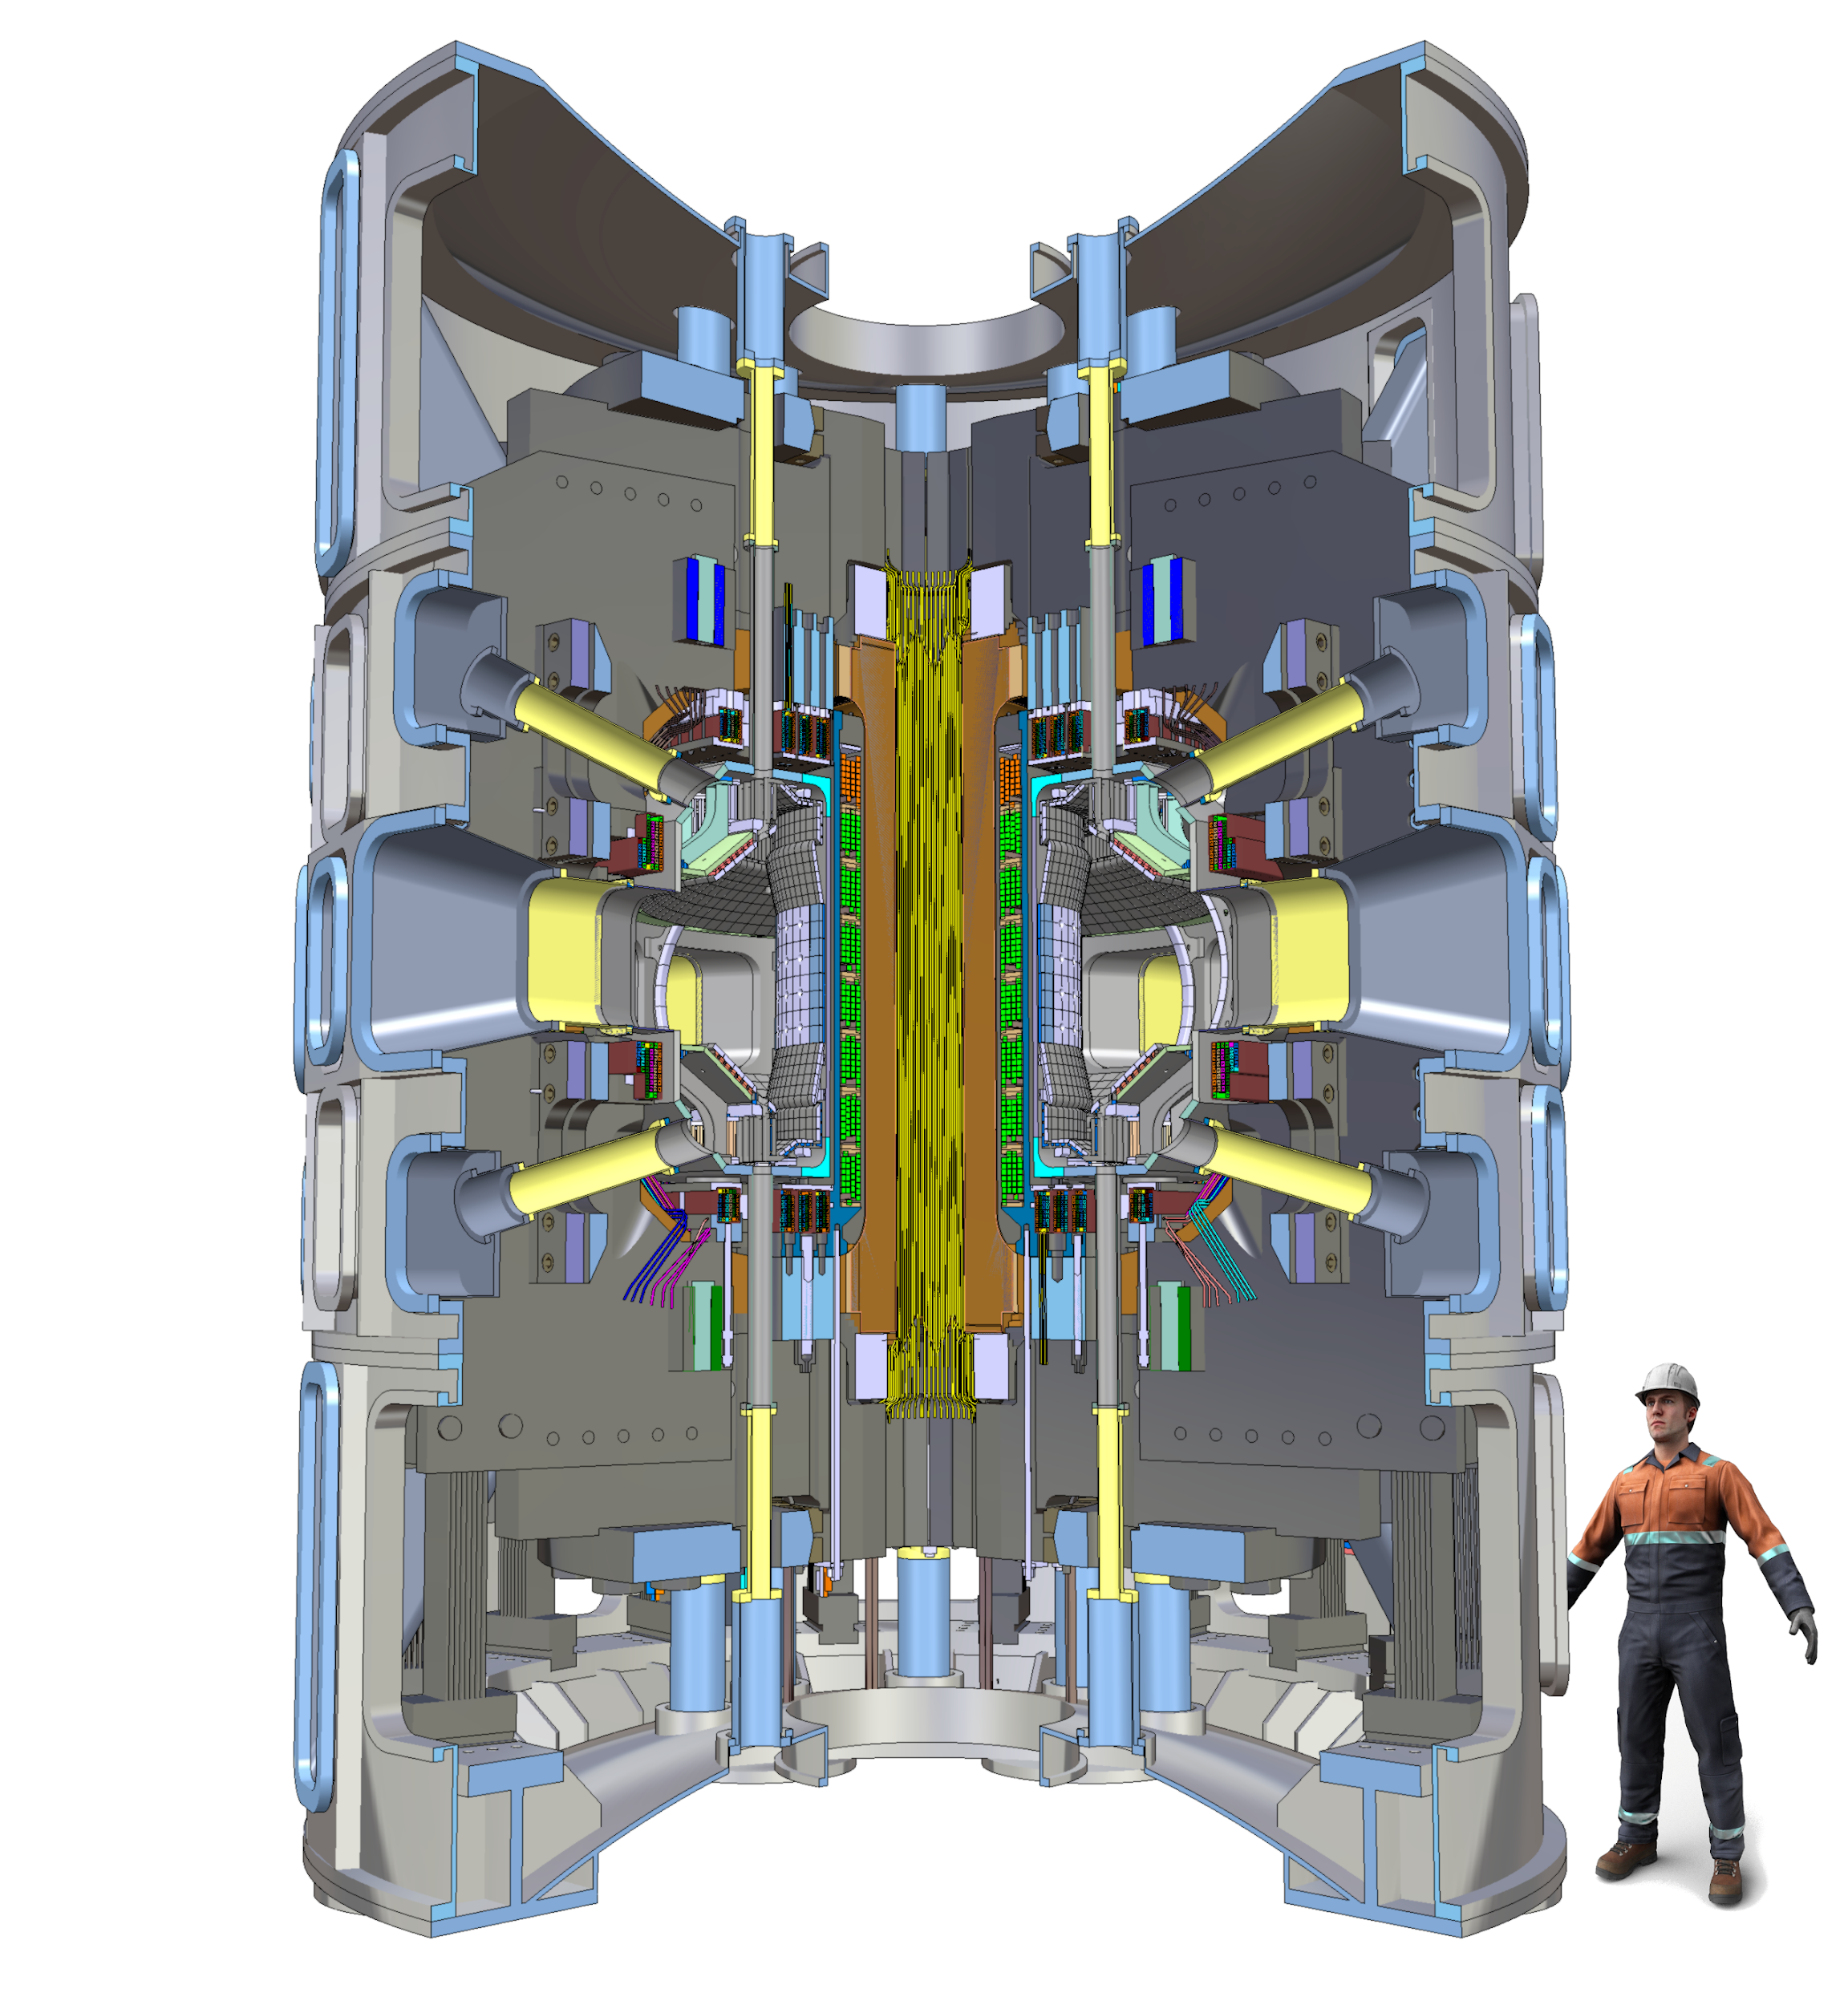
\includegraphics[width=8cm]{compass_u.png}
  \centering
  \caption{Schematic cross-section of the COMPASS-U tokamak.}
  \label{fig:compass}
\end{figure}

COMPASS-U is designed to operate at a toroidal magnetic field of up to $B_t = 5~T$ and a plasma current of $I_p = 2~MA$, with a major radius of $R = 0.894~m$ and a minor radius of $a = 0.27~m$.
The device offers a highly flexible magnetic configuration, allowing operation in single-null, double-null, snowflake and negative triangularity plasma scenarios.
A key feature of the machine is its closed, reactor-relevant divertor, designed to achieve high neutral compression and high plasma density, enabling experimental studies of detached plasma operation under conditions approaching those expected in ITER and DEMO.
The facility will also serve as a European test bed for advanced plasma-facing components, including liquid metal divertor concepts, while providing an experimental platform for investigations of edge plasma physics, advanced confinement regimes such as QH-mode, I-mode and negative triangularity plasmas, as well as disruption physics and power exhaust relevant for future fusion power plants.


\pagebreak
\subsection{Commercial fusion research}
Commercial fusion development has accelerated rapidly during the last decade. Companies pursue both tokamak and stellarator concepts, often combining compact reactor geometries with high-temperature superconducting magnets and shorter engineering development cycles than publicly funded programmes. The following examples illustrate engineering approaches that are particularly relevant to the development of future high-heat-flux components and reactor technologies.

\subsubsection{Tokamak: Tokamak Energy}

Tokamak Energy is a private fusion company founded in 2009 in the United Kingdom as a spin-out from Culham fusion research. The company focuses on the development of compact spherical tokamaks combined with high-temperature superconducting (HTS) magnets. Compared to conventional tokamaks, spherical tokamaks exhibit a much lower aspect ratio, resulting in a more compact plasma configuration. This concept is expected to improve plasma performance while reducing the overall size and cost of future fusion power plants.
A key technological focus of Tokamak Energy is the application of REBCO high-temperature superconducting tapes for the construction of toroidal field magnets. These conductors enable magnetic fields exceeding those achievable with conventional low-temperature superconductors while operating at higher temperatures around 20 K. Stronger magnetic fields substantially improve plasma confinement and allow the reactor dimensions to be reduced. According to the Lawson scaling, increasing the magnetic field strength has a significantly greater impact on fusion performance than increasing the plasma volume, making HTS technology one of the main engineering directions pursued by the company.
The company's experimental program has progressed through several prototype devices, including ST25 and ST40 (Figure \ref{fig:st40}). 
\begin{figure}[h]
  \centering
      \centering
      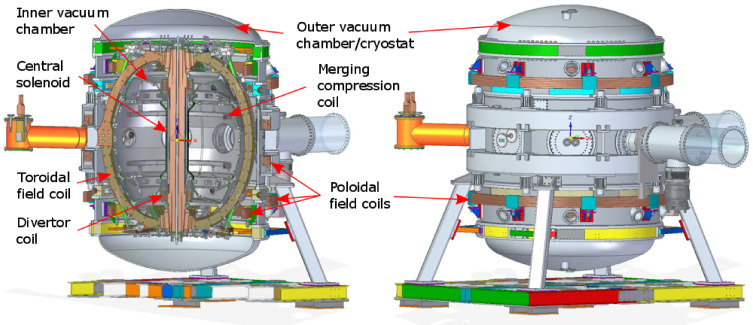
\includegraphics[height=6cm]{st_40.jpg}
      \caption{ST-40 design schematic \cite{st40}.}
      \label{fig:st40}
\end{figure}
The ST40 tokamak achieved plasma temperatures above 100 million degrees Celsius, demonstrating that compact spherical tokamaks can reach reactor-relevant temperature conditions. In 2026, Tokamak Energy continued operating ST40 as a fusion-technology platform while completing a 14-month campaign on its Demo4 HTS magnet system; the company reported a peak field of 13.7~T and used the programme to validate integrated HTS technology for fusion applications \cite{TokamakEnergy2026}. Current research is focused on integrating high-field superconducting magnets with advanced plasma control systems and on demonstrating long-pulse operation required for future power plants.
Unlike publicly funded research programmes centred on ITER and DEMO, Tokamak Energy follows a commercial development strategy with shorter design cycles and rapid prototyping. The long-term objective is to translate the compact spherical-tokamak and HTS-magnet technology into a pilot fusion power-plant concept. Besides fusion energy, the company is also developing high-temperature superconducting magnet technology for applications outside the fusion sector, including medical imaging, particle accelerators and industrial systems. Consequently, the commercialization of HTS technology represents an important intermediate milestone independent of the successful realization of a commercial fusion reactor.

\pagebreak
\subsubsection{Tokamak: Commonwealth Fusion Systems and SPARC}
Commonwealth Fusion Systems (CFS), founded as a spin-out from the Massachusetts Institute of Technology, is constructing the SPARC compact high-field tokamak in Devens, Massachusetts. SPARC uses high-temperature superconducting REBCO magnets and is intended to demonstrate a burning plasma with a fusion gain above unity. As of 2026, construction and subsystem commissioning are proceeding in parallel; CFS reported the machine to be almost 80~\% complete, with production toroidal-field magnets being installed and major support systems entering operation \cite{CFS2026SPARC}. SPARC is a demonstration device rather than a power plant; its results are intended to provide the physics and engineering basis for the subsequent ARC power-plant programme.

\subsubsection{Stellarator: Renaissance Fusion}
Renaissance Fusion is promising a new approach to fusion technology with innovations that simplify traditional designs while increasing efficiency. A key advancement lies in the use of simple coil surfaces to generate the complex 3D magnetic fields required for stellarators. Instead of intricate, hard-to-manufacture coils, Renaissance Fusion uses 1D or 2D coils, often placed on cylindrical surfaces, to create the necessary magnetic fields. This design decouples the engineering from the physics, making construction easier and more scalable.
\\
\\
\noindent The company also focuses on the use of high-temperature superconductors (HTS) to generate the strong magnetic fields needed for effective plasma confinement. Traditional HTS manufacturing involves complex steps like producing tapes or cables, but Renaissance Fusion skips these steps, directly depositing and patterning HTS on large surfaces. This approach could make HTS more cost-effective, which is crucial for compact fusion reactors. A 4x increase in magnetic field strength reduces the reactor size by 256x, allowing for smaller, more efficient fusion devices.
Another innovation is the use of thick, flowing liquid lithium walls to manage neutron energy and heat in the reactor. These walls absorb 99.99~\% of neutron energy, preventing damage to solid materials and reducing radioactive contamination. The liquid also acts as a coolant, transferring heat to turbines for electricity generation, and it aids in tritium breeding, which is necessary for fuel production. With these innovations, Renaissance Fusion is addressing key challenges in fusion energy, aiming to make reactors smaller, cheaper, and more efficient.
\begin{figure}[ht]
  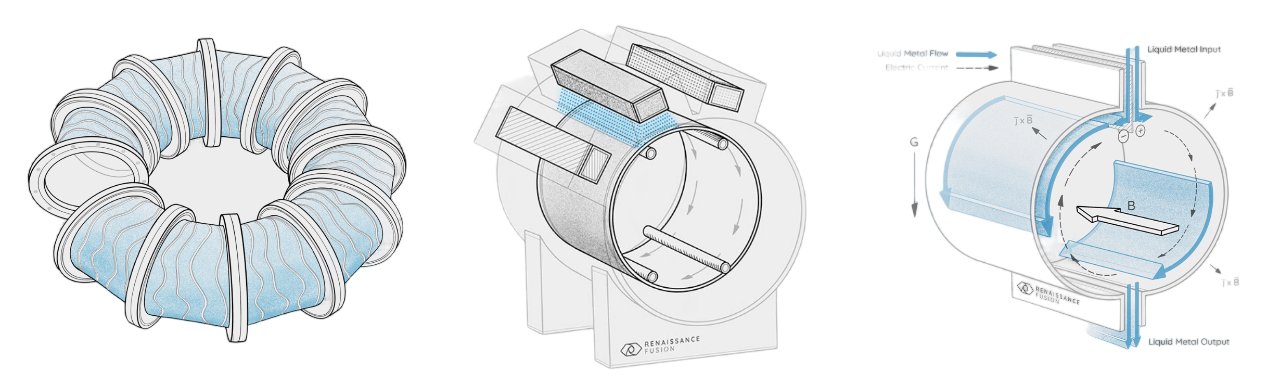
\includegraphics[width=15cm]{RF.png}
  \centering
  \caption{The three main conceptual aspects of the Renaissance Fusion design \cite{renfusion_technology_2024}.}
  \label{fig:rf}
\end{figure}
\noindent Renaissance fusion approach to develop the first prototype of a fully functional fusion power plant introduces new technologies in all of the main components design.
The aim to ship the first small nuclear fusion reactor by the early 2030s is very optimistic, as it is in the case of majority of commercial fusion companies.
However, the main technological challenges can be utilized on a broad spectrum of fields such as: MRI scanner construction or energy storage systems.
From this point of view, the economical sustainability of Renaissance Fusion in the future may be in patents and technologies for non-fusion applications. 
To date, the company has also published 6 articles in peer-reviewed journals describing the developed technologies \cite{Fam2024}.

\subsubsection{Stellarator: Proxima Fusion and Alpha}
Proxima Fusion is a commercial stellarator company spun out of the Max Planck Institute for Plasma Physics (IPP). Its development programme builds directly on the optimized-stellarator knowledge established by Wendelstein~7-X. In February 2026, Proxima Fusion, IPP, the Free State of Bavaria and RWE announced a framework for the construction of the \textit{Alpha} demonstration stellarator in Garching, with IPP providing the scientific leadership \cite{IPPProximaAlpha2026}. Alpha is intended as a net-energy-gain demonstrator and as an engineering step towards the proposed \textit{Stellaris} commercial stellarator power plant.

\pagebreak
\section{Power exhaust in nuclear fusion devices}
Nuclear fusion devices are experiencing heat loads that are very rarely found in any other engineering field.
One of the case with comparable heat load is the heat load on rocket shields during the re-entry to the Earth atmosphere \cite{Park2021}.
Its important to note that the rocket shields experience high thermal load only for a very limited amount of time, compared to the fusion reactor first wall.
In general, high heat fluxes can be divided in three categories based on its magnitude \cite{Woodcock2019,Ebadian2011}.
\begin{itemize}
  \item HHF - \textbf{High heat flux} = 1--10~MW/m$^2$
  \item UHF – \textbf{Ultra-high heat flux} = 10--100~MW/m$^2$
  \item EHF – \textbf{Extreme heat flux} > 100~MW/m$^2$

\end{itemize}

\subsection{ITER and DEMO}

The DEMO project is a significant step from experimental fusion facilities towards full-scale fusion power plants. The aim of DEMO is to use the experience and technology from ITER to build a tokamak capable of delivering electricity to the transmission grid. The cooling system on the DEMO tokamak will have the task of transferring the thermal power released by the fusion reaction (in this case the projected 2 GW) to the turbine and generators as efficiently as possible. 
In addition to the current technical challenges of fusion power in the areas of heat resistant materials, plasma control, or sufficient heat dissipation, the DEMO project has complications such as the complications between pulsed tokamak operation and continuous turbine operation. With the successful operation of the DEMO plant (planned in 2044), the final step will be the PROTO project, a fully operational prototype fusion power plant.
The cooling cycle of the DEMO plant has several different concept designs.

\subsubsection{First wall radiative heat load}

Figures \ref{fig:mapatoku1} and \ref{fig:mapatoku2} show the expected heat flux profile on the cross section of ITER torus. 
Modules of the FW panels are divided in two groups: normal and enhanced heat flux regions.
The heat flux values represent the steady state radiative heat load without any plasma disruptions and ELMs.

\begin{figure}[h]
  \centering
  \begin{minipage}{0.70\textwidth}
      \centering
      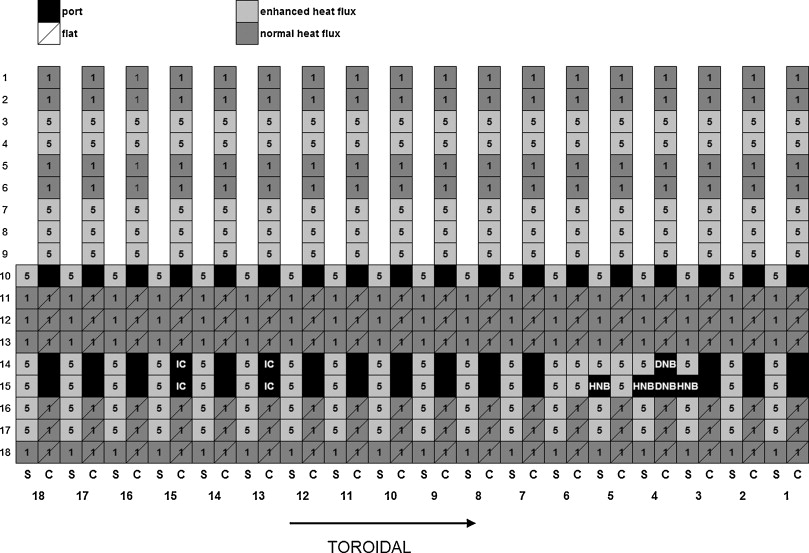
\includegraphics[width=\linewidth]{mapa_load.jpg}
      \caption{Distribution map of all BMs. The black squares are the ports or openings. Light gray squares are panels with 5~MW.m$^{-1}$ capability, dark gray with 1~MW.m$^{-1}$ capability \cite{Mitteau2010}.}
      \label{fig:mapatoku1}
  \end{minipage}\hfill
  \begin{minipage}{0.25\textwidth}
      \centering
      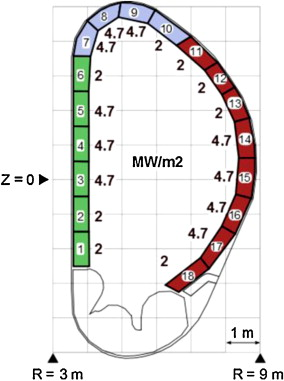
\includegraphics[width=\linewidth]{profil_load.jpg}
      \caption{Steady state design heat flux for ITER FW panels \cite{Merola2014-zi}.}
      \label{fig:mapatoku2}
  \end{minipage}
\end{figure}

\pagebreak
\noindent The instabilities of the plasma operation can lead to a significant local heat load increase (10--100~MW/m$^2$) for a short period of time.
Figure \ref{fig:mapatoku3} shows the expected heat flux profiles on the cross section of DEMO torus for two heat load distribution assumptions. 
The first case in the Figure \ref{fig:mapatoku3}(left) shows the heat load on the first wall of DEMO for a plasma total radiative power of 457~MW, based on the assumption of a constant radiation source density on flux surfaces: The radial radiation source profiles have been obtained DEMO simulations with STRAHL [29] coupled to ASTRA [30, 31]
The second case in the Figure \ref{fig:mapatoku3}(right) shows the radiation load on the first wall of DEMO based on the assumption that 150~MW of power is radiated from the x-point.
Those two cases show how the relation between the radiative power source and the heat load profile distribution.

\begin{figure}[h]
  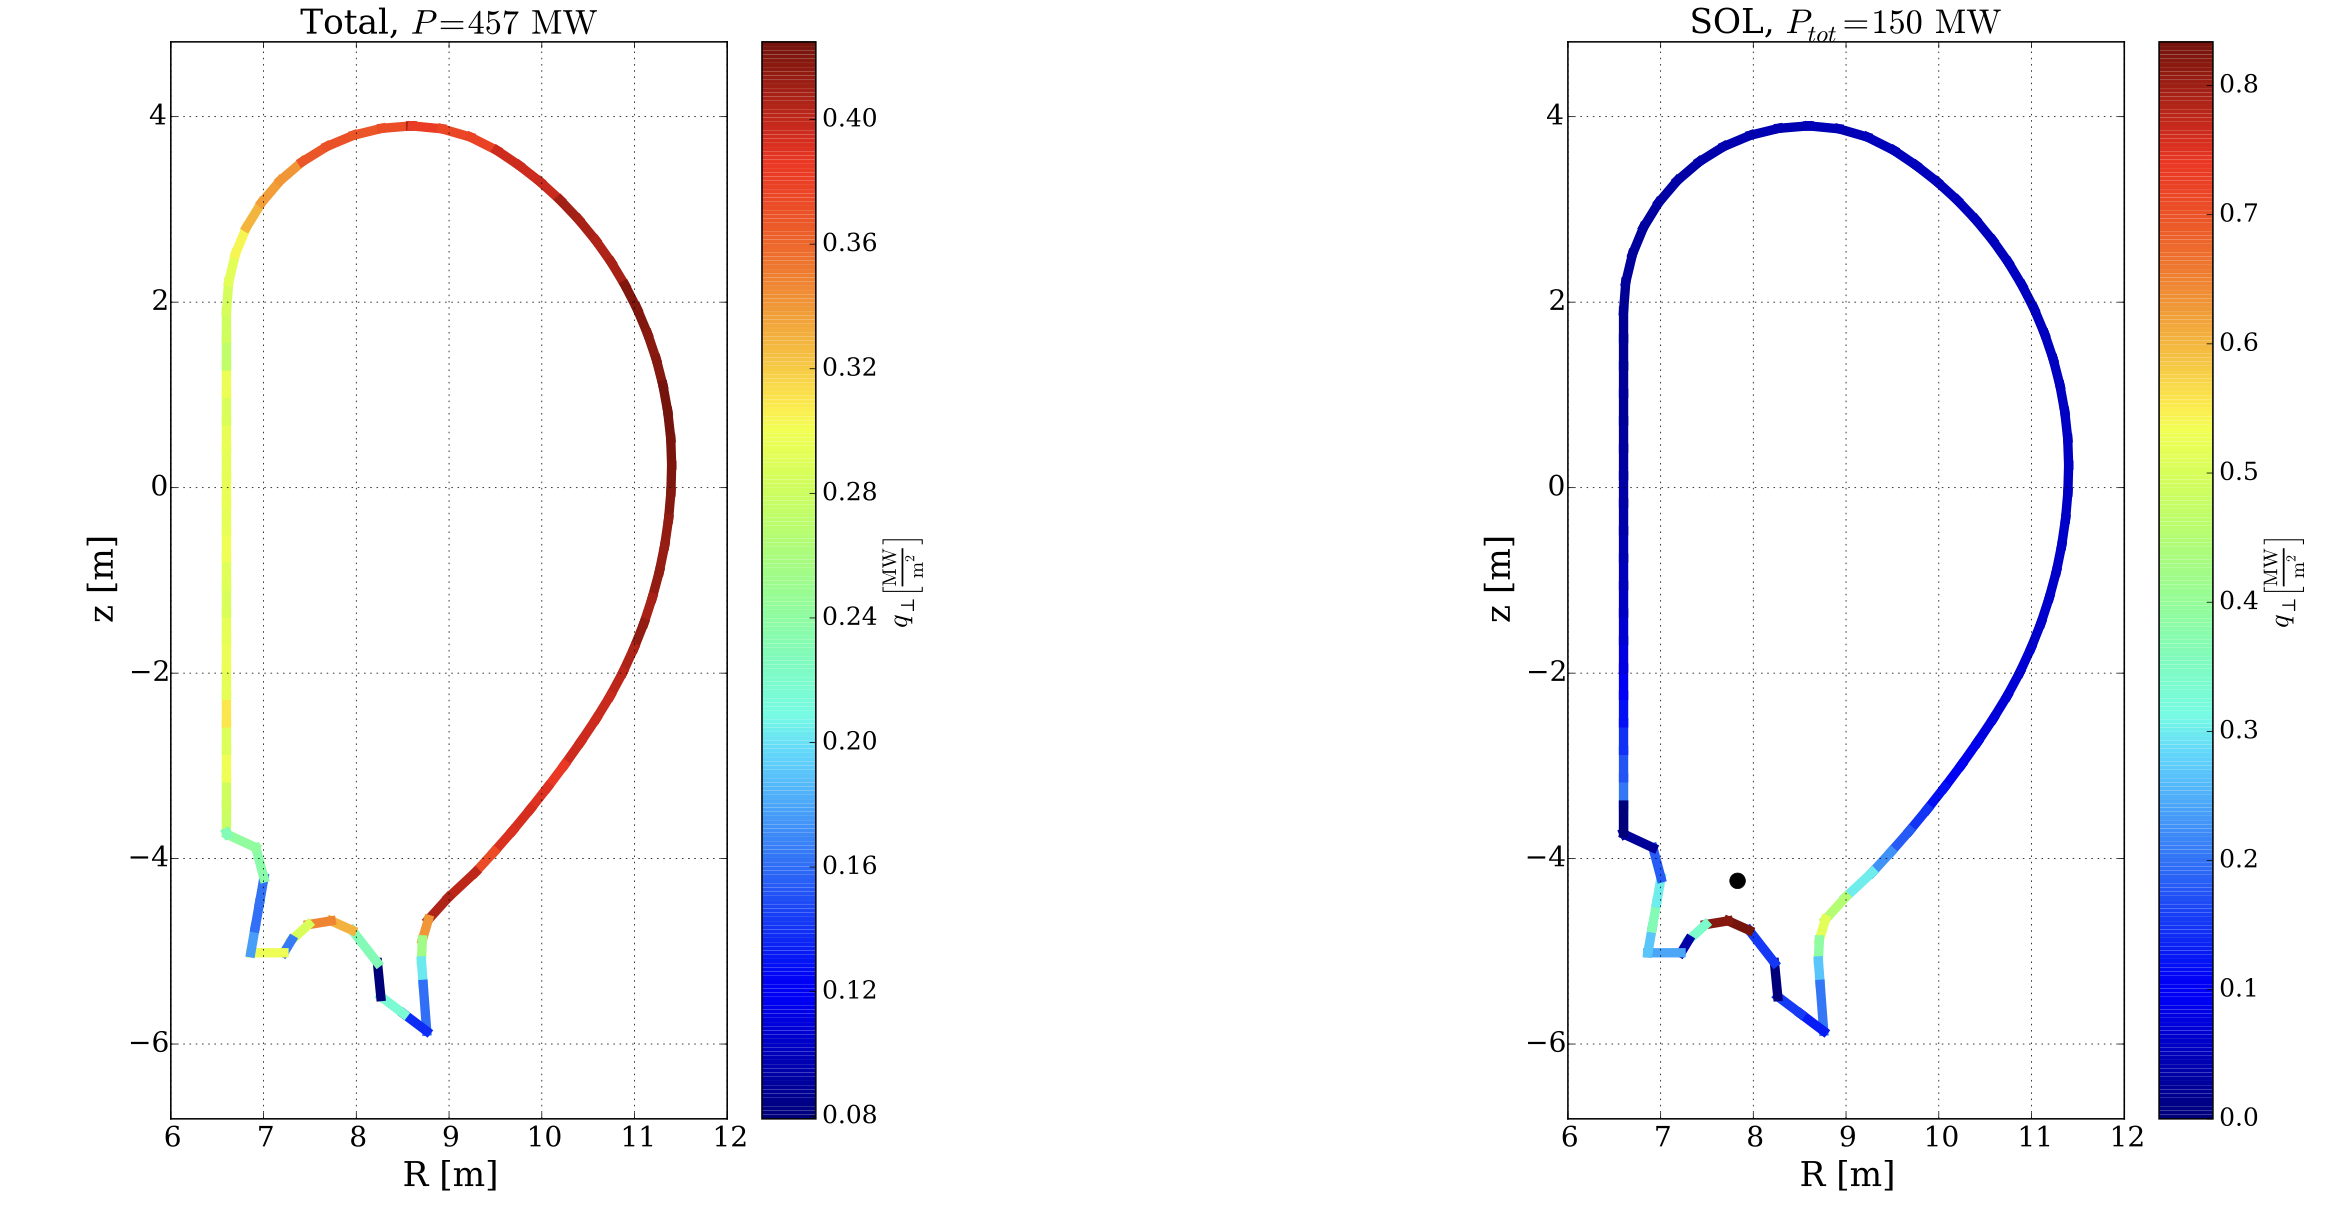
\includegraphics[width=15cm]{DEMO_load.png}
  \centering
  \caption{Radiative heat load distribution in DEMO cross section \cite{Wenninger_2017}.}
  \label{fig:mapatoku3}
\end{figure}

\noindent It is important to note that both heat load cases mentioned in Figure \ref{fig:mapatoku3} take into account only a fraction of the total expected DEMO power of 2000~MW, therefore the heat load in DEMO first wall are going achieve higher values.
The total power of 457~MW in the first case represents the total charged particle heating power (alpha heating power and auxiliary heating power) \cite{Wenninger_2017}.
Heat loads lower than 10~MW.m$^{-1}$ can be sufficiently cooled by FW panels based on the hypervapotron water cooled channel \cite{Ciric}.
Higher loads caused by disruptions and ELMs are expected to last only around 10.$^{-3}$s, therefore the initiated heat wave can be fully absorbed by the mass of the FW pannel.


\subsubsection{Divertor convective heat load}

The highest steady-state heat loads during normal tokamak operation occur on the divertor targets. ITER divertor plasma-facing components are designed for local steady-state heat fluxes of the order of 10~MW/m$^2$, substantially above the nominal first-wall load.
Figure \ref{fig:mapatoku4} shows the order of magnitude of both the power density (heat flux) and the pulse duration of: divertor load, disruptions, edge localized modes (ELMs) and vertical displacement events (VDEs).
Figure \ref{fig:mapatoku5} shows an example of the ITER divertor target surface temperature response to a 1 ms ELM during the operation, indicating the melting of a tungsten target surface can clearly occur during those extreme events. 
Designing FW component able to exhaust a steady state high heat flux without any structural damage is one of the main engineering challenges of nuclear fusion research and development.
One of the innovative solutions for withstanding those extremely high local heat flux conditions is the introduction of liquid metal divertor target. 
The layer of molten metal is held on the first wall by he capillary effect \cite{Horacek}.


\begin{figure}[h]
  \centering
  \begin{minipage}{0.5\textwidth}
      \centering
      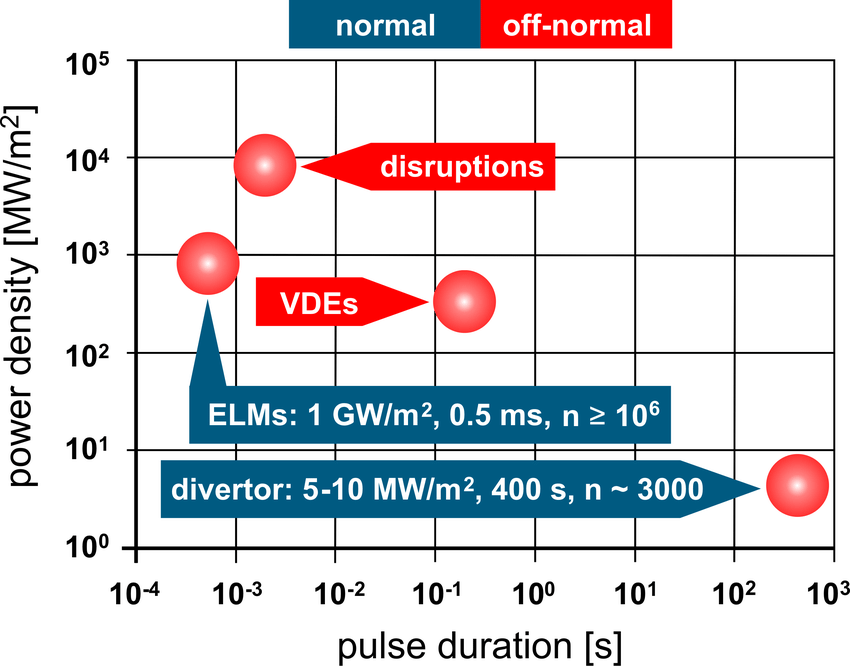
\includegraphics[width=\linewidth]{Thermal-loads-on-the-divertor.png}
      \caption{Expected thermal loads on the ITER divertor \cite{Loarte2003-zo}\cite{Li2019}.}
      \label{fig:mapatoku4}
  \end{minipage}\hfill
  \begin{minipage}{0.45\textwidth}
      \centering
      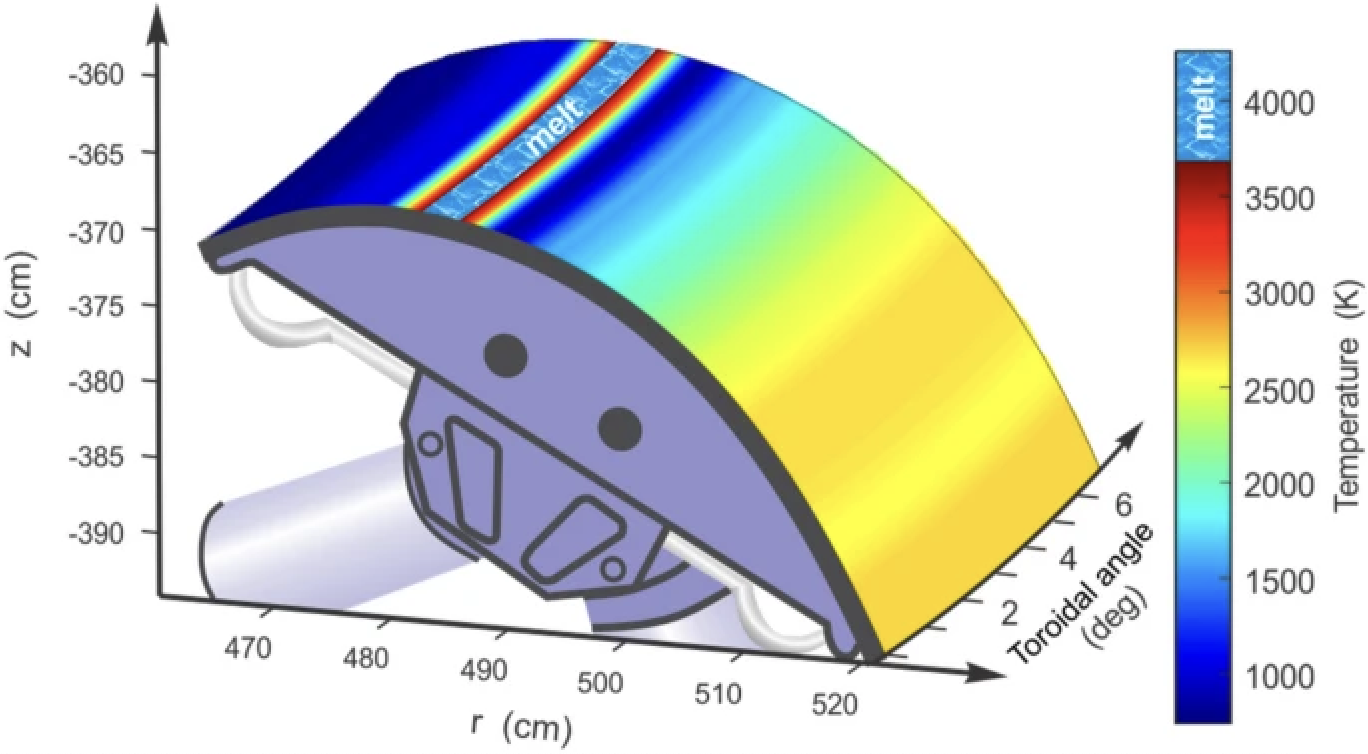
\includegraphics[width=\linewidth]{div_load.png}
      \caption{Thermal response of the ITER Dome surface after the 1.0 ms ELM \cite{Hassanein2021-cg}.}
      \label{fig:mapatoku5}
  \end{minipage}
\end{figure}


\pagebreak

\paragraph{Scope of the cooling discussion.}
The plant-level heat-rejection and power-conversion systems of ITER and DEMO are not discussed in detail here because the present thesis focuses on local heat removal from plasma-facing components. The relevant design point is that first-wall, divertor and vacuum-vessel cooling circuits operate under different thermal and hydraulic requirements; therefore, the local cooling-channel geometry has to be evaluated independently of the overall balance-of-plant architecture.

\pagebreak

\subsection{Wendelstein-7x heat load analysis}
Cooling of plasma facing components in research fusion reactors is described in comparison to the challenges designing a full scale fusion power plant.
In the case of Wendelstein 7-X, the first wall heat shields are installed in areas where its necessary to protect diagnostic systems from the plasma heat load.
As shown in Figure \ref{fig:w7xpohled}, the plasma facing components are divided in several categories with variable ranges of expected heat load levels: the test divertor units (TDU, $\leq$10~MW/m$^2$), the baffles (500~kW/m$^2$), heat shields and toroidal closures and ($\leq$500~kW/m$^2$) at the stainless steel wall panels.
Stainless steel wall (with no heat shield) is present in the regions where the diagnostic systems dont require heat shielding.
Some graphite heat shield tiles are equipped with tungsten coating.
The cooling systems are also designed to provide the baking function, heating the vacuum chamber up to 150~$^\circ$C for a long period of time \cite{Endrychova2026}.
\\
\\
\noindent The specification of design loads for in-vessel components sets a reference heat load for the plasma facing heat shields to 250~kW/m$^2$ of uniform steady state load.
Graphite tiles of heat shields are actively cooled by water flow in stainless steel pipes, CuCrZr heat sinks provide thermal connection and structural support between the cooling pipes and the graphite tiles.
The cooling water inlet temperature is around 30~$^\circ$C.
As the design of W7-X is very irregular, each heat shield has a bit different cooling properties.
In general, the water mass flow through the cooling pipe is around 0.4 to 1 kg.s$^{-1}$ , the expected dT for the 250~kW/m$^2$ design load is 15-30~$^\circ$C per each heat shield \cite{Dhard2017}.

\begin{figure}[h]
  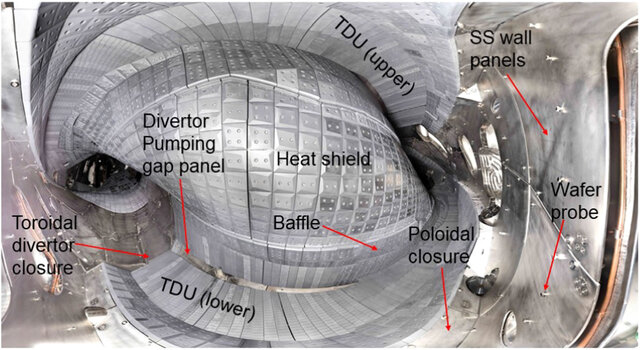
\includegraphics[width=15cm]{Panorama-view-into-the-W7-X-plasma-vessel-from-W7-X-module-4-showing-the-installed_W640.jpg}
  \centering
  \caption{View into W7-X plasma vessel from module 4, showing the installed plasma facing components \cite{Dhard2020}.}
  \label{fig:w7xpohled}
\end{figure}

\noindent Heat load on the surface of plasma facing component can be divided in three main groups: plasma radiative heat load, plasma convective heat load and the load created by plasma heating systems (NBI, ECRH).
Radiative load targets all surfaces in the view angle of plasma, convective loads (deposited by charged particles) are found locally on baffles and divetor targets.
Power generated by the plasma heating systems such as NBI and ECRH can shine through the plasma (or the systems may be tested on an empty vessel without plasma), discharging the heat flux directly on the first wall.
Heating systems are built to generate a significant power, thus the fusion devices should be equipped with safety measures to prevent any damage to the first wall in the case of malfunction.

\subsubsection{Radiative load}

Figure \ref{fig:w7xzaznam} shows the power measurement during one of the W7-X pulses. 
$P_{ECRH}$ represents the heating power of electron cyclotron resonance heating and $P_{rad}$ is the measured radiative power of plasma.
The selected W7-X pulse 20230209.019 shows that the majority of incoming ECRH heating power was released from plasma in a form of radiation, the difference between the curves represents the non-radiative convective loads.
The closer the curves are to each other, the smaller the convective loads are.

\begin{figure}[h]
  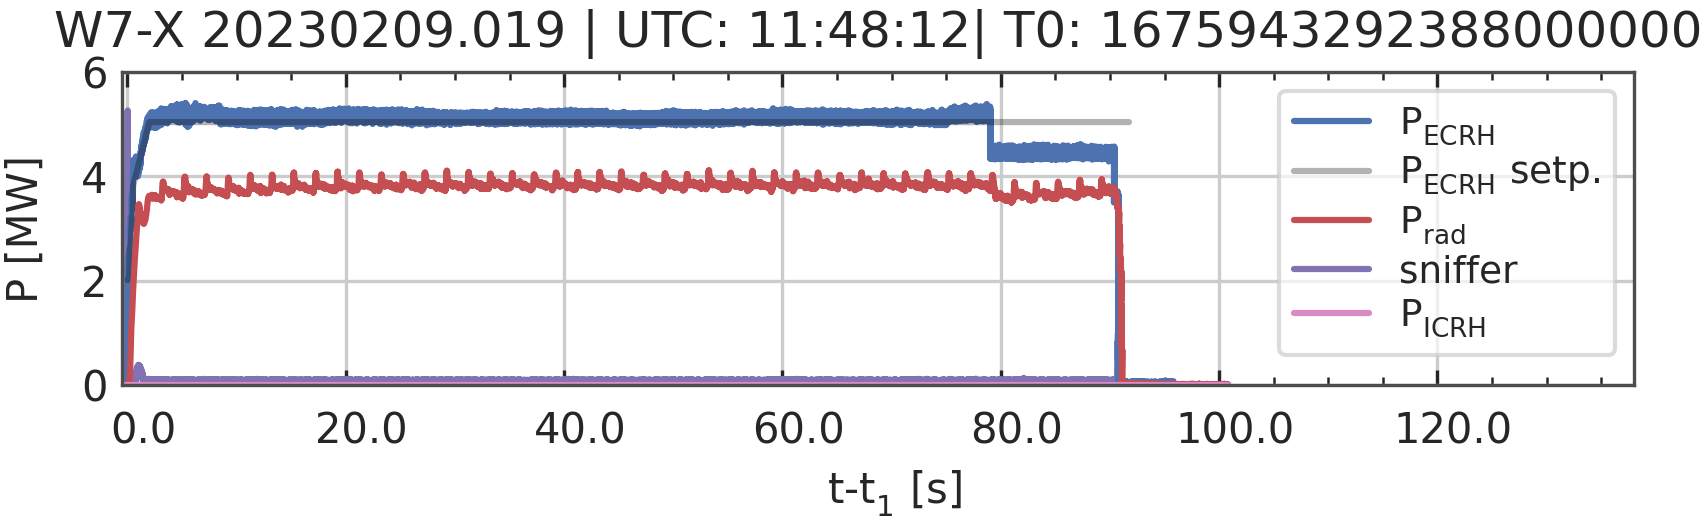
\includegraphics[width=14cm]{zaznam_vykonu.png}
  \centering
  \caption{W7-x power measurement during the pulse \cite{Grulke2024}.}
  \label{fig:w7xzaznam}
\end{figure}

\noindent The total value of radiated power can be used to estimate the heat flux load on the first wall surfaces through the following method.
In the case of perfectly toroidal tokamak, the total radiative power can be simply divided by the torus surface.
For more complex geometries of tokamaks and stellarators, shape of the plasma surface and the FW geometry needs to be considered.
The geometry of the last closed plasma surface (seen in blue color in the Figure \ref{fig:imagestell1}) and the plasma facing FW surfaces are used in a ANSYS Mechanical FEA simulation to estimate the heat load profile.
Radiative heat flux between two surfaces with temperatures $T_{\mathrm{plasma}}$ and $T_{\mathrm{FW}}$ is expressed by the Stefan–Boltzmann law (Equation \ref{eq:radiace}).
Using this equation, the temperature of the plasma surface can be calculated in relation to the fixed value of FW temperature (22~$^\circ$C ambient temperature) for the selected value of resulting heat flux.
Setting the FW surfaces as thin 2D shell elements and emissivities $\epsilon$ to 1 allows us to run the surface to surface radiosity solver (Figure \ref{fig:radiace}) \cite{Dublin_Misha}.

\begin{equation}
  q = \sigma \cdot \epsilon \cdot \frac{\left(T_{\mathrm{plasma}}^4-T_{\mathrm{FW}}^4\right)}{2-\epsilon}
  \label{eq:radiace}
\end{equation}
where $q$ is the net radiative heat flux, $\sigma$ is the Stefan--Boltzmann constant, $\epsilon$ is the assumed surface emissivity and $T_{\mathrm{plasma}}$ and $T_{\mathrm{FW}}$ are the equivalent radiating-surface and first-wall absolute temperatures, respectively.

\begin{figure}[h]
  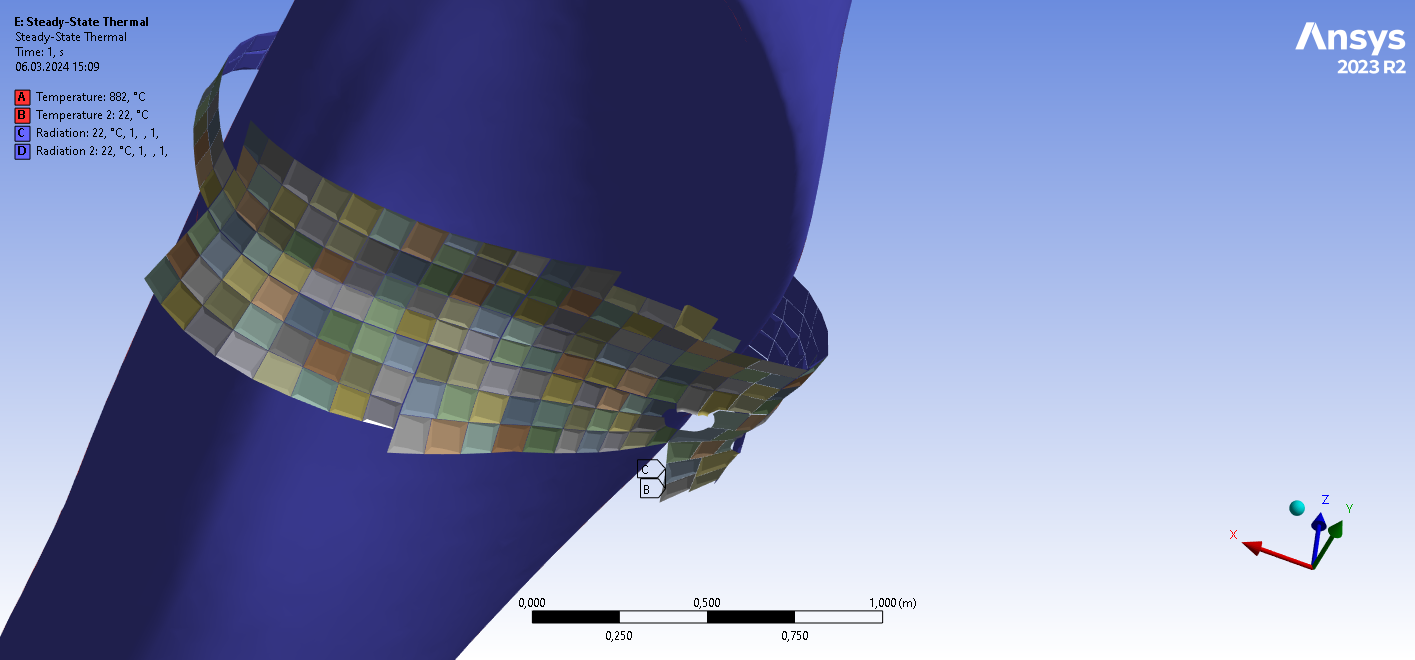
\includegraphics[width=13cm]{image6.png}
  \centering
  \caption{Last magnetic surface and the first wall shell 2D elements of Abschirmhaus HM 31/40.}
  \label{fig:radiace}
\end{figure}

\pagebreak

\noindent Figure \ref{fig:w7xtokprofil} shows an example of heat flux profile in the region of Abschirmhaus of half module 31/40.
This simplified method of heat flux profile calculation is helpful in the heat load evaluation and the design of plasma facing components.

\begin{figure}[h]
  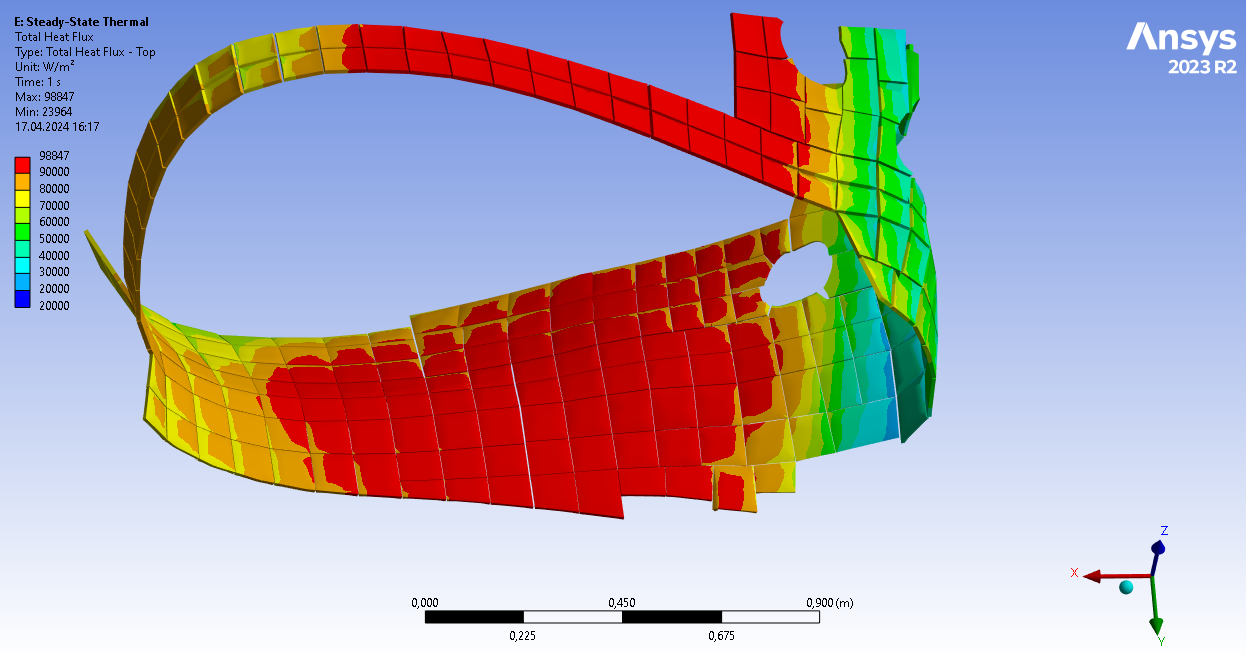
\includegraphics[width=13cm]{image9.png}
  \centering
  \caption{W7x cross section heat load profile.}
  \label{fig:w7xtokprofil}

\end{figure}

\subsubsection{Convective load}

An example of convective load observed on the baffle is shown in Figure \ref{fig:baffle}.
Heat flux reached up to 1~MW/m$^2$, approximately ten times larger than the heat shield's radiative load. This significant disparity underscores the dominance of convective heat transfer in certain regions of the reactor, particularly in areas exposed to direct plasma interaction. The baffle, designed to manage and redirect plasma flows, experiences intense localized heating due to the high-energy particles and turbulent plasma behavior in its area. 

\begin{figure}[h]
  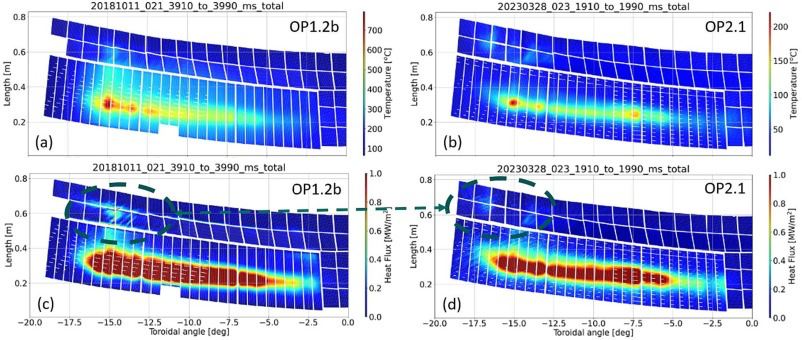
\includegraphics[width=15cm]{convective_load.png}
  \centering
  \caption{Comparison of surface temperature and heat load patterns for the different baffle designs as used in OP1.2b and OP2.1 experiment campaigns.}
  \label{fig:baffle}
\end{figure}

\pagebreak
\subsubsection{NBI beam load}
Neutral Beam Injection (NBI) is one of the plasma heating system.
The beam of neutralized particles is able to deliver energy through the magnetic field into the plasma.
A part of the beam energy can pass through the plasma to the first wall, increasing the heat load in the targeted "beam dump" area.
In the case of empty vessel with no plasma or NBI beam/diagnostic testing, the beam may be targeted directly to the beam dump area with full power.
Figure \ref{fig:nbi_port} shows the interaction of NBI beam with port of its origin and the beam dump area.

\begin{figure}[h]
  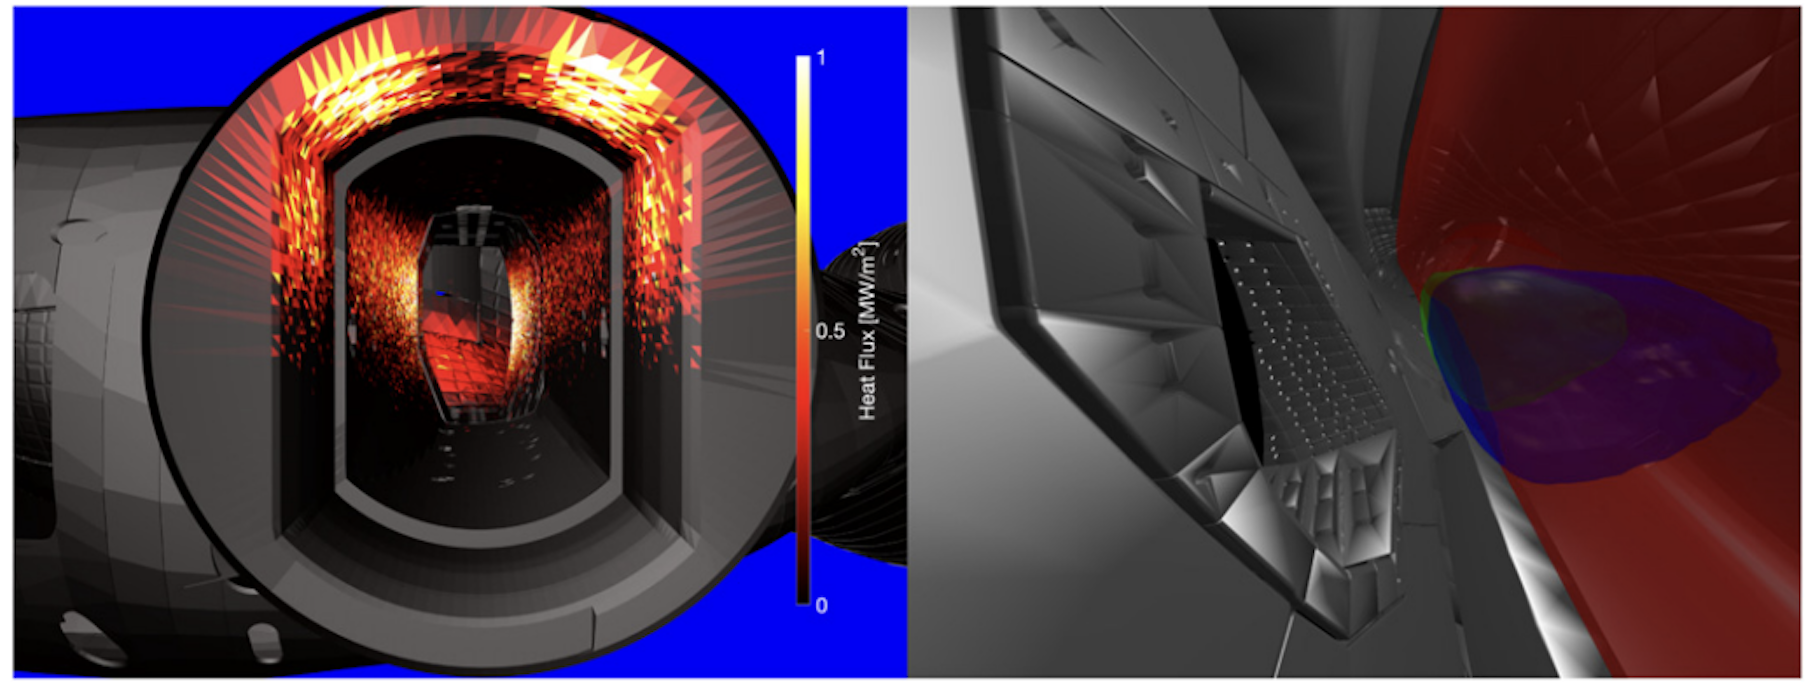
\includegraphics[width=13cm]{nbi_sam.png}
  \centering
  \caption{Solution of NBI simulation in BEAMS3D. Model geometry includes port interaction (left) and the beam dump area (right) \cite{Lazerson2021}.}
  \label{fig:nbi_port}
\end{figure}

\noindent The NBI load to heat shield surface can be calculated by particle simulations such as BEAMS3D, an example of heat load profile and magnitude created by NBI beam shot in an empty vessel is shown in Figure \ref{fig:nbi_dump}.
Two NBI sources (S3 and S4) with a power of 1.8~MW per source create a beam dump area with an average load around 12~MW/m$^2$ on targeted tiles.
Circa 3.1~MW of the total 3.6~MW are loaded to the beam dump area, the remaining fraction of heating power is deposited on the NBI port itself.
Beam dump area heat shields are under the highest heat load in the device.
ECRH heating source also creates an area of increased heat flux on the first wall, a specially designed ECRH reflector tiles are installed on W7-X for this purpose \cite{olive-leriche2024}.

\begin{figure}[h]
  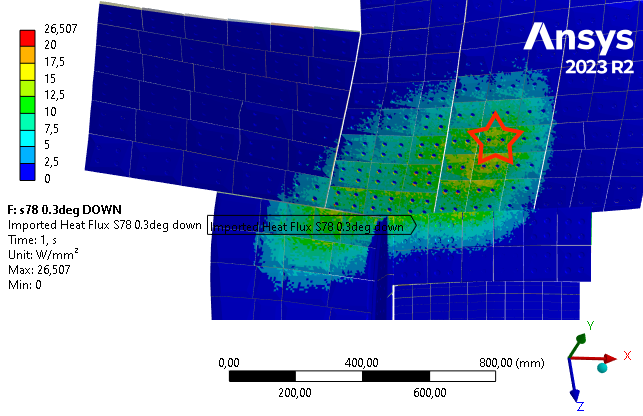
\includegraphics[width=11cm]{novy_profil.png}
  \centering
  \caption{W7-x NBI Beam dump area heat load. Sources s78 are shifted in a downward direction from the nominal position to include assembly imperfections.}
  \label{fig:nbi_dump}
\end{figure}

\pagebreak
\subsubsection{Structural limits of plasma facing components}

Mechanical stresses induced in material by the large temperature gradients under high heat fluxes are one of the primary concern in the plasma facing component design.
An example of first wall design in the W7-X is a graphite tile in the beam dump area, where the risk of structural damage poses a greater threat than the thermal risk of high temperatures.
The selected tile is marked by a red star in Figure \ref{fig:nbi_dump}.
The heat flux profile with an average value of 12~MW/m$^2$ per plasma facing graphite face is shown in detail in Figure \ref{fig:nbi_tile1}.

\begin{figure}[h]
  \centering
  \begin{minipage}{0.5\textwidth}
      \centering
      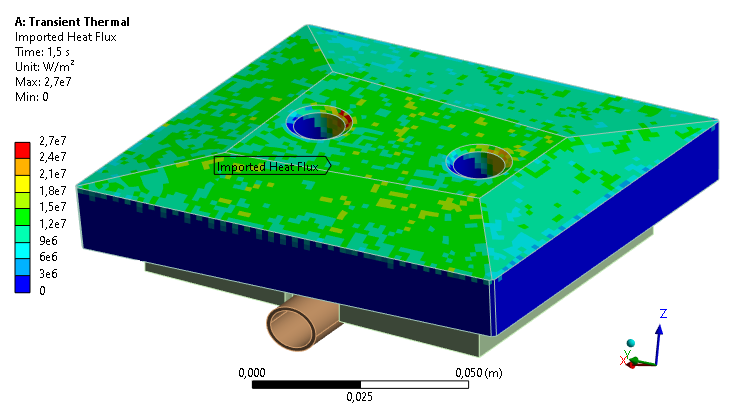
\includegraphics[width=\linewidth]{load.png}
      \caption{Heat flux load \cite{Dublin_vojta}.}
      \label{fig:nbi_tile1}
  \end{minipage}\hfill
  \begin{minipage}{0.5\textwidth}
      \centering
      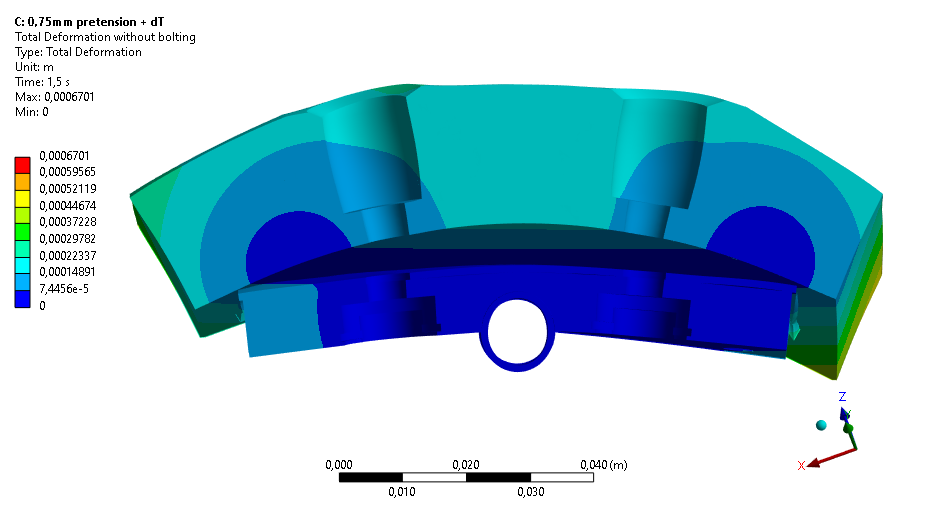
\includegraphics[width=\linewidth]{bend.png}
      \caption{Structural deformation (50x)\cite{Dublin_vojta}}
      \label{fig:nbi_tile2}
  \end{minipage}
\end{figure}

\noindent In 1.5 seconds of NBI beam heating, the maximal temperature in the graphite body reaches up to 2700~$^\circ$C.
Figure \ref{fig:nbi_tile3} shows a large temperature gradient through the graphite tile.
As a result of thermal expansion, "the bending effect" is observed (Figure \ref{fig:nbi_tile2}), causing a significant stress in the bolted connection between graphite tile and CuCrZr heat sink.
This mechanical stress can lead to damage of the NBI targeted tile in a short period of heat load.

\begin{figure}[h]
  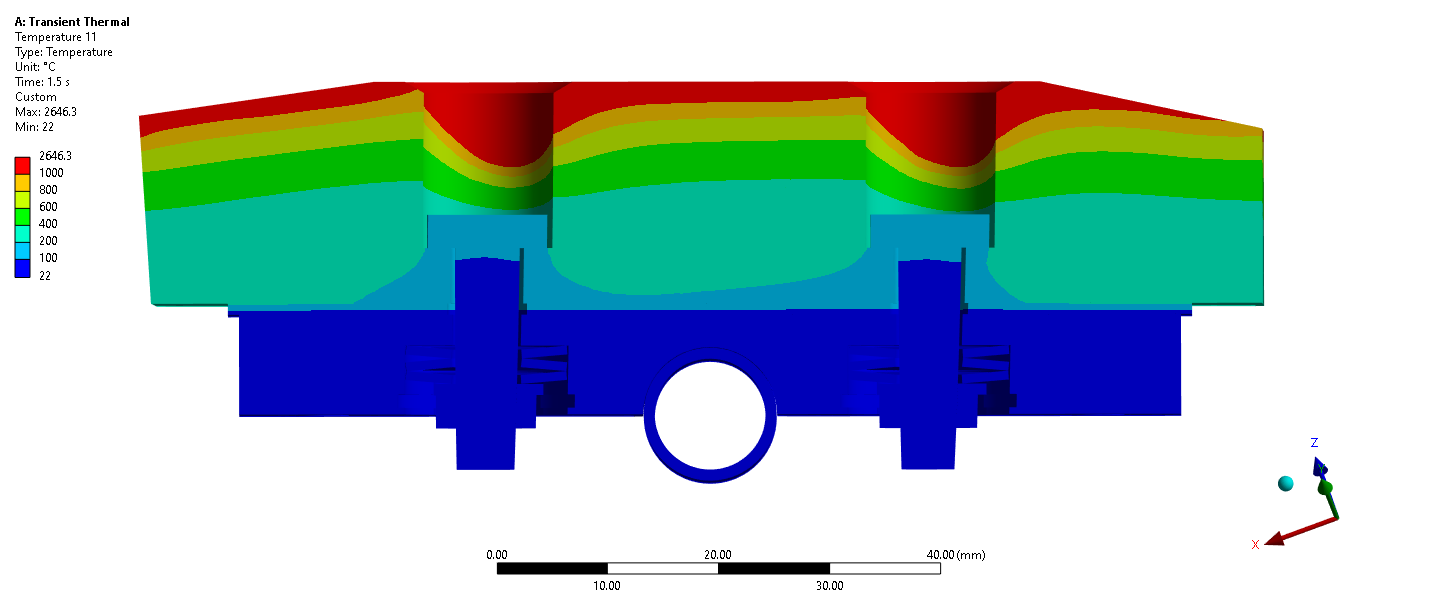
\includegraphics[width=15cm]{image1.png}
  \centering
  \caption{Temperature profile of the W7x NBI beam dump graphite tile after being targeted for 1.5 s by the NBI heat load \cite{Dublin_vojta}.}
  \label{fig:nbi_tile3}
\end{figure}

\noindent For plasma-facing components, the challenge lies in balancing plasma-wall interactions, high melting points, and thermal conductivity, necessitating the use of multiple materials between the plasma and the cooling fluid.
However, the joints between these materials often present structural limitations that fall short of the thermal constraints (melting point).
Plasma-facing materials can also be protected by deposited refractory-metal coatings, particularly tungsten, to reduce erosion of the underlying substrate and limit the release of impurities into the plasma \cite{Dublin_bety}.


\pagebreak
\section{Cooling channel geometries applied in nuclear fusion}
This chapter reviews water-cooled channel geometries used for plasma-facing components (PFCs) in fusion devices. Blanket design and tritium-breeding concepts are outside the scope of the present work; only the local heat-removal geometry between the plasma-facing surface and coolant is considered.
The two primary geometries, also used in the design of the ITER tokamak, are the swirl tube for divertor target cooling and the hypervapotron for cooling the first wall modules \cite{Baxi}.

\subsection{Swirl tube}
The swirl tube is defined by a twisted tape installed inside the cooling pipe.
This design enhances heat transfer by inducing a swirling motion in the cooling fluid, which increases turbulence and improves thermal contact between the fluid and the tube walls. 
The spiral flow pattern that maximizes surface area contact and thus optimizes heat removal.
In fusion reactors like ITER, swirl tube cooling is critical due to the extreme thermal loads faced by divertor targets.
By improving heat transfer efficiency, the swirl tube design allows for more compact cooling systems and better temperature control, compared to the plain tube geometry.
Figure \ref{fig:ST_1} shows the ITER divertor target design, the swirl tube is shown in detail in Figure \ref{fig:ST_2}.
\\
\\
\noindent An extensive numerical study was performed by M. Ghambalez to estimate the optimal twist of the swirl tube tape to achive the highest heat transfer efficiency in relation to the operating conditions.
The study involves numerical simulations examining the effects of twisted tape inserts with various design parameters—twisted tape pitch, truncation percentage, and positioning—on the heat transfer and flow characteristics in tubes. The results show that reducing the twisted tape pitch significantly enhances the heat transfer, with lower pitch values like L/4 achieving the highest improvement in the Nusselt number (up to 151.42~\% at a Reynolds number of 1000). Additionally, truncating the twisted tape reduces both heat transfer and pressure drop, with the best thermal performance observed when the tape is positioned at the tube entrance. These insights help optimize heat exchanger designs for improved energy efficiency \cite{Ghalambaz2020}.

\begin{figure}[h]
  \centering
  \begin{minipage}{0.5\textwidth}
      \centering
      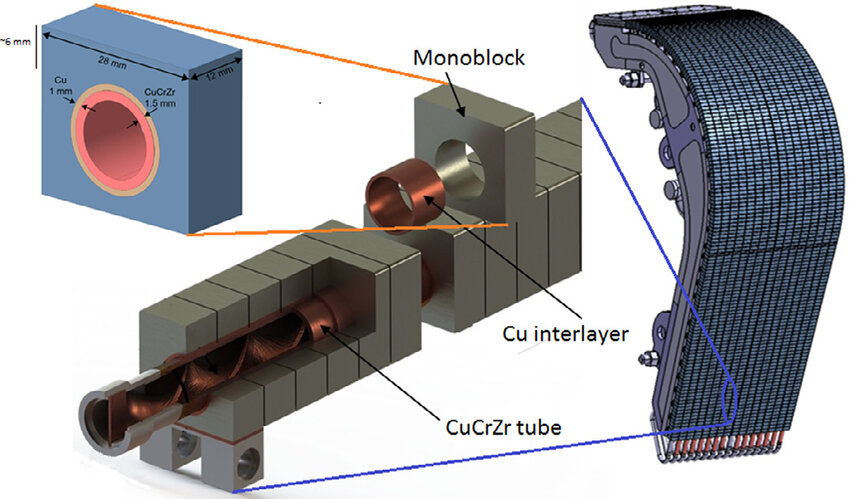
\includegraphics[width=\linewidth]{swirl_tube_geom.jpeg}
      \caption{Divertor vertical target geometry, ITER.}
      \label{fig:ST_1}
  \end{minipage}\hfill
  \begin{minipage}{0.5\textwidth}
      \centering
      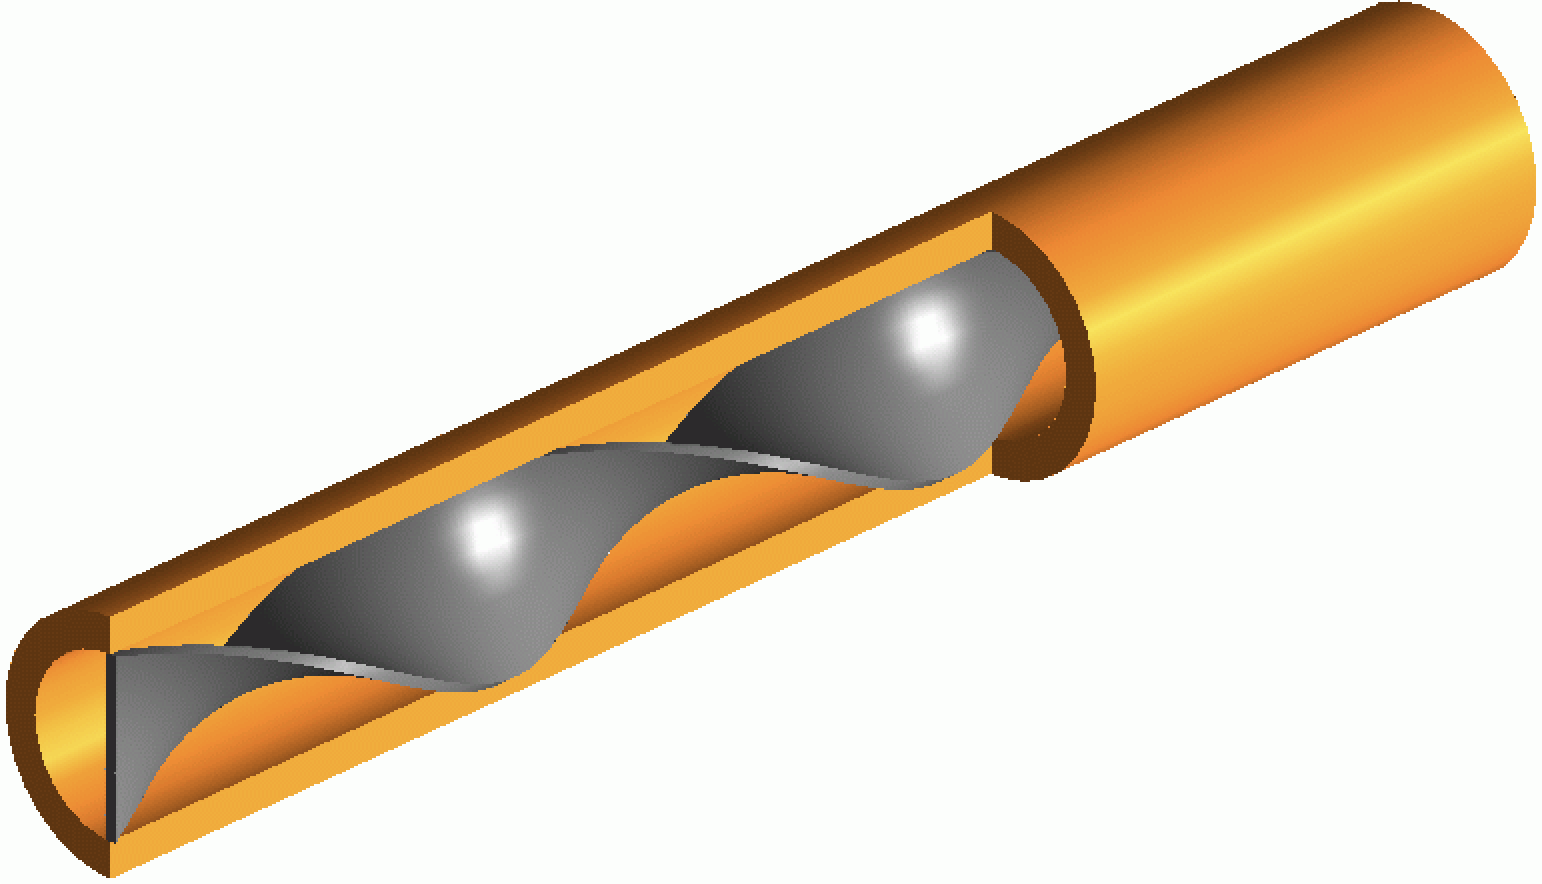
\includegraphics[width=\linewidth]{st_tape.png}
      \caption{Swirl tube geometry.}
      \label{fig:ST_2}
  \end{minipage}
\end{figure}

\noindent A recent article by Xiangyu Li presents an experimental and computational study investigating the critical heat flux (CHF) in cooling systems under high-pressure conditions. Using an electron beam to simulate plasma thermal loads, the experiment was conducted with varying flow rates and subcooling levels, with CHF values measured using acoustic methods. CFD simulations were also carried out using ANSYS FLUENT to validate these findings. 
The results show that the dilution rates significantly impact CHF, with lower mass flow rates reducing CHF values. The study also found that subcooling does not linearly affect CHF; higher subcooling increases CHF, while lower subcooling leads to more effective heat transfer due to wider subcooled boiling areas. The simulation results deviated up to 32~\% from experimental data, but the overall accuracy was within acceptable limits \cite{Li2022}.



\pagebreak
\subsection{Hypervapotron}
Subcooled boiling represents an important physical phenomenon for high heat flux cooling. 
It occurs when the liquid near the heated surface reaches boiling, while the temperature of the main body of the liquid remains below the boiling point (saturation temperature, $T_{\mathrm{sat}}$). As a result, vapor bubbles form but collapse back into liquid before reaching the surface. In the case of a flowing liquid, these vapor bubbles collapse within the main liquid stream, enhancing the overall heat transfer from the hot surface to the cooling liquid. Subcooled boiling provides higher heat flux for a given temperature difference compared to single-phase convection \cite{Lim2021}.
\\
\\
\noindent Stable subcooled boiling, close to the maximum (critical) heat flux, can be achieved by optimizing the combination of channel geometry and liquid properties.
The fin geometry promotes recirculation and nucleate boiling inside the slots, increasing heat removal from the heated wall.
The term "vapotron" refers to a channel with cooling fins designed to enhance heat transfer from the heated wall to the cooling liquid. In a "supervapotron," the cooling fins are aligned parallel to the liquid's forced flow, allowing for a maximum heat flux of 3~MW/m$^2$. 
By narrowing the gaps between the fins, this heat flux can be increased to 5~MW/m$^2$. In a "hypervapotron," the cooling fins are arranged perpendicular to the liquid flow, a design that promotes more intense vapor production in the slots and enables heat fluxes up to 20~MW/m$^2$.
\begin{figure}[h]
  \centering
  \begin{minipage}{0.5\textwidth}
      \centering
      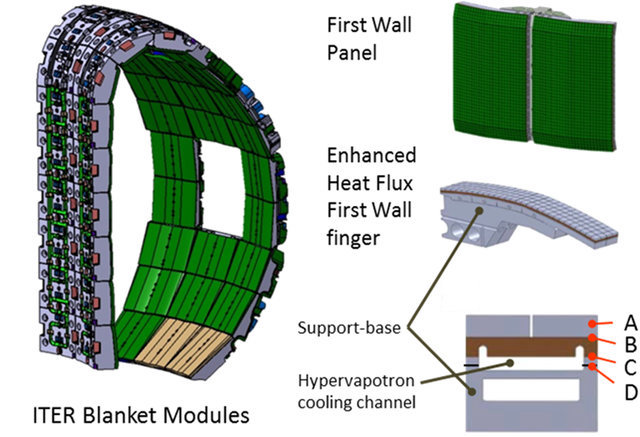
\includegraphics[width=\linewidth]{iter_cooling.jpg}
      \caption{ITER first wall module cooling, the hypervapotron channel \cite{Hirai2016}.}
      \label{fig:hypervapotron1}
  \end{minipage}\hfill
  \begin{minipage}{0.5\textwidth}
      \centering
      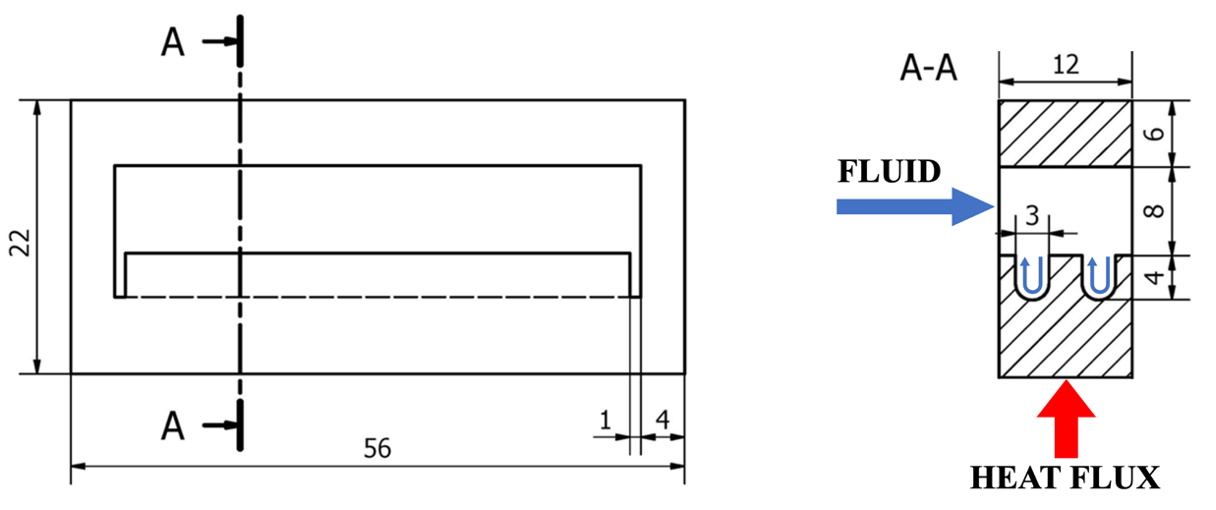
\includegraphics[width=\linewidth]{hypervapo.png}
      \caption{Hypervapotron geometry \cite{Smolk2023}.}
      \label{fig:hypervapotron2}
  \end{minipage}
\end{figure}

Figure \ref{fig:hypervapotron2} illustrates the most common type of hypervapotron geometry, showing the flow between the fins. These fins can take various shapes—rectangular, triangular, sinusoidal, or others—but are always perpendicular to the liquid flow. Although some experiments have explored angled fins, perpendicular fins remain the primary focus of research and development.
The shown geometry corresponds to the hypervapotrons used in the JET tokamak at Culham, as well as the ITER tokamak. In JET, hypervapotrons serve as beam-stopping elements in both the Neutral Beam Injectors and the Neutral Beam Test Bed. These cooling channels are typically made from CuCrZr alloy.
Figure \ref{fig:hypervapotron1} shows how the hypervapotron is integrated in the ITER first wall design.

\subsection{Alternative solutions}
As the hypervapotron and the swirl tube are already tested technology with known limits, several advanced techniques have been developed to improve heat transfer and increase the critical heat flux limit.
One promising technique is the addition of ice particulates to the cooling water. This method significantly enhances heat transfer by maximizing the subcooling effect, as the ice melts and absorbs heat. Tests conducted under specific conditions—such as 2~bar water pressure and a 30~\% ice fraction—have shown that this approach can manage heat fluxes up to 20~MW/m$^2$\cite{Gorbis1993}.

\begin{figure}[h]
  \centering
  \begin{minipage}{0.45\textwidth}
      \centering
      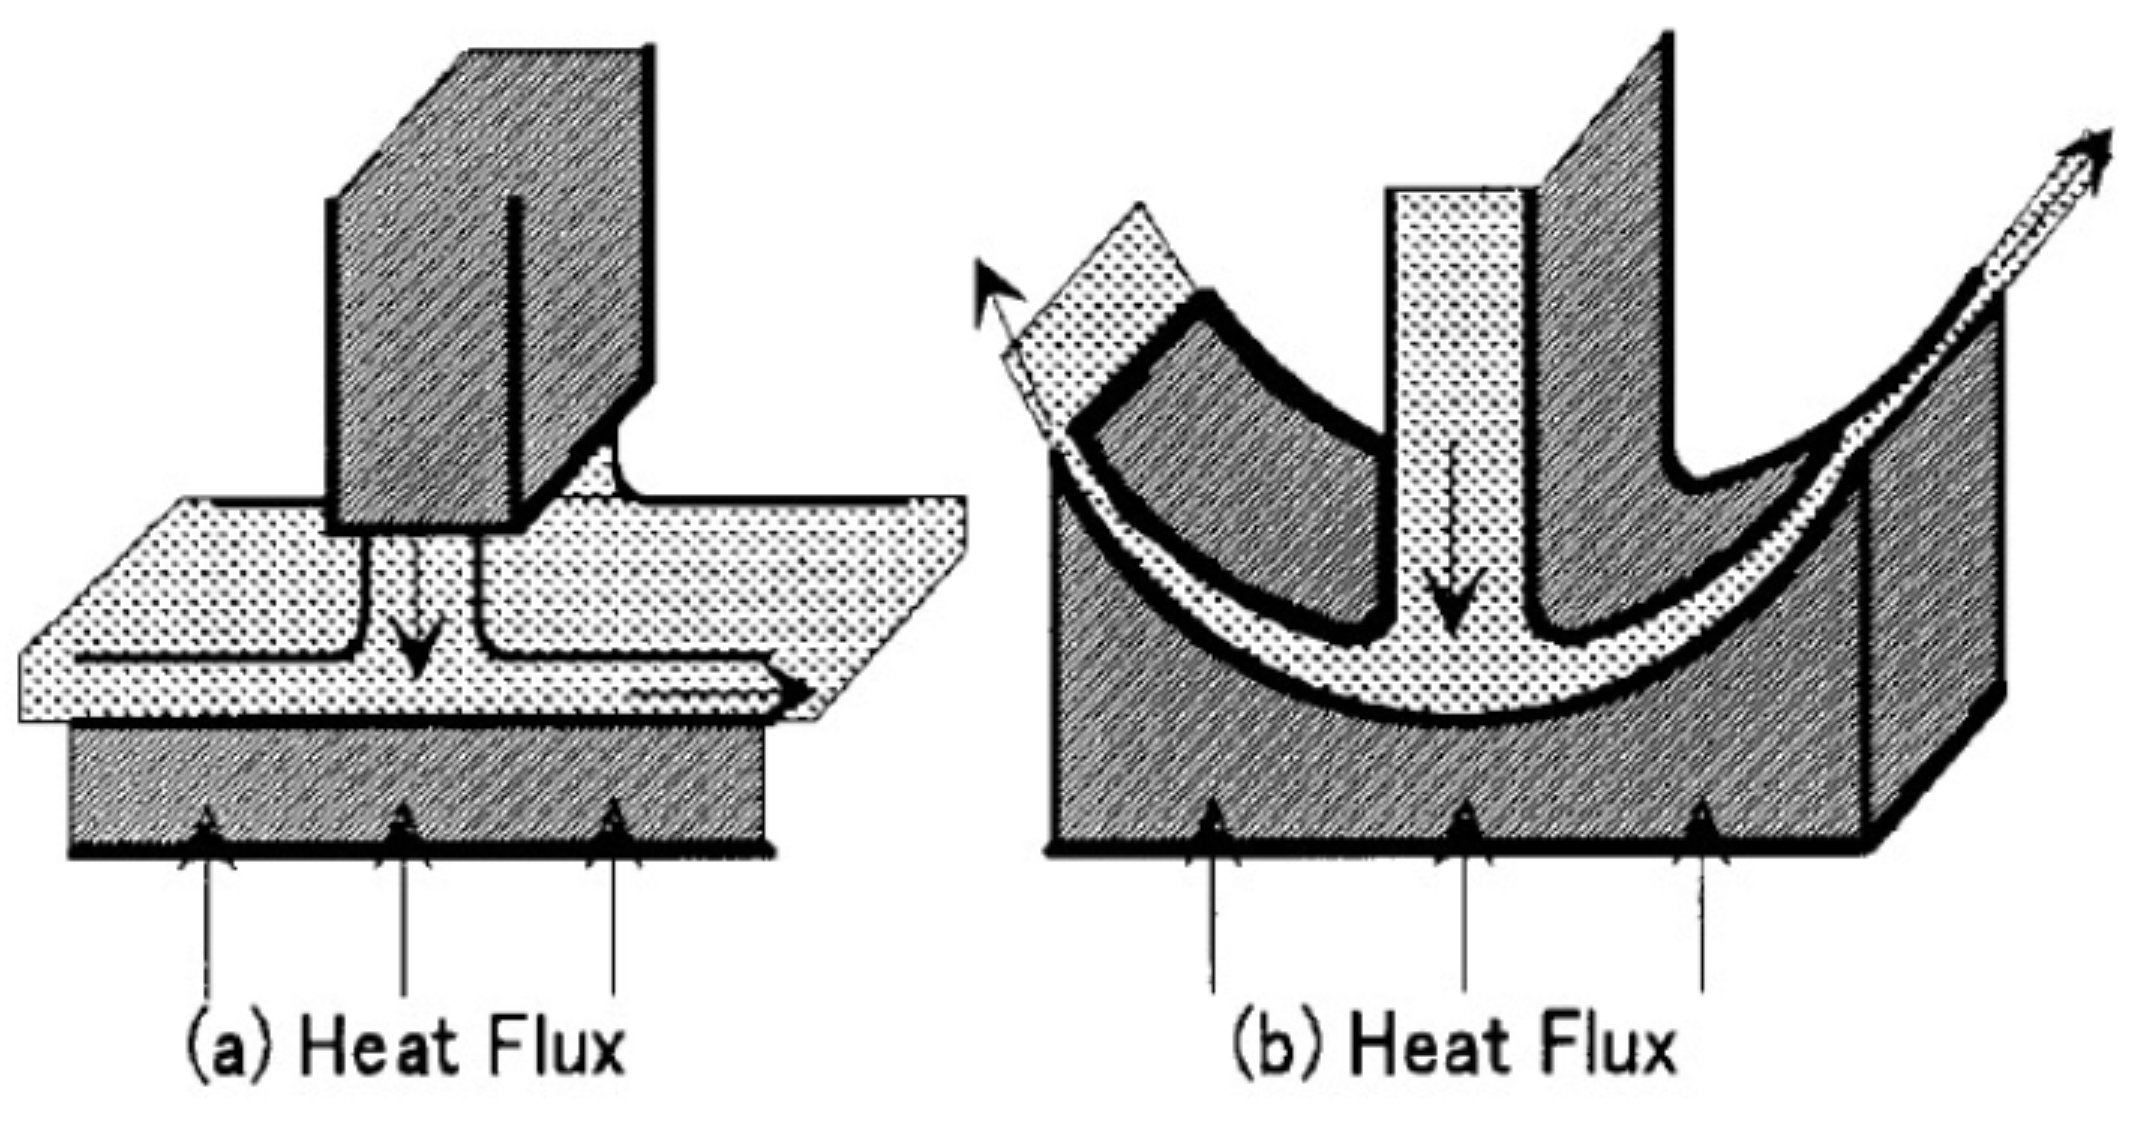
\includegraphics[width=\linewidth]{alternative_HF1.png}
      \caption{Various systems for impinging planar jetcooling: (a) a free jet on a flat surface. (b) a confinedjet on a curved surface \cite{Inoue2000}.}
  \end{minipage}\hfill
  \begin{minipage}{0.4\textwidth}
      \centering
      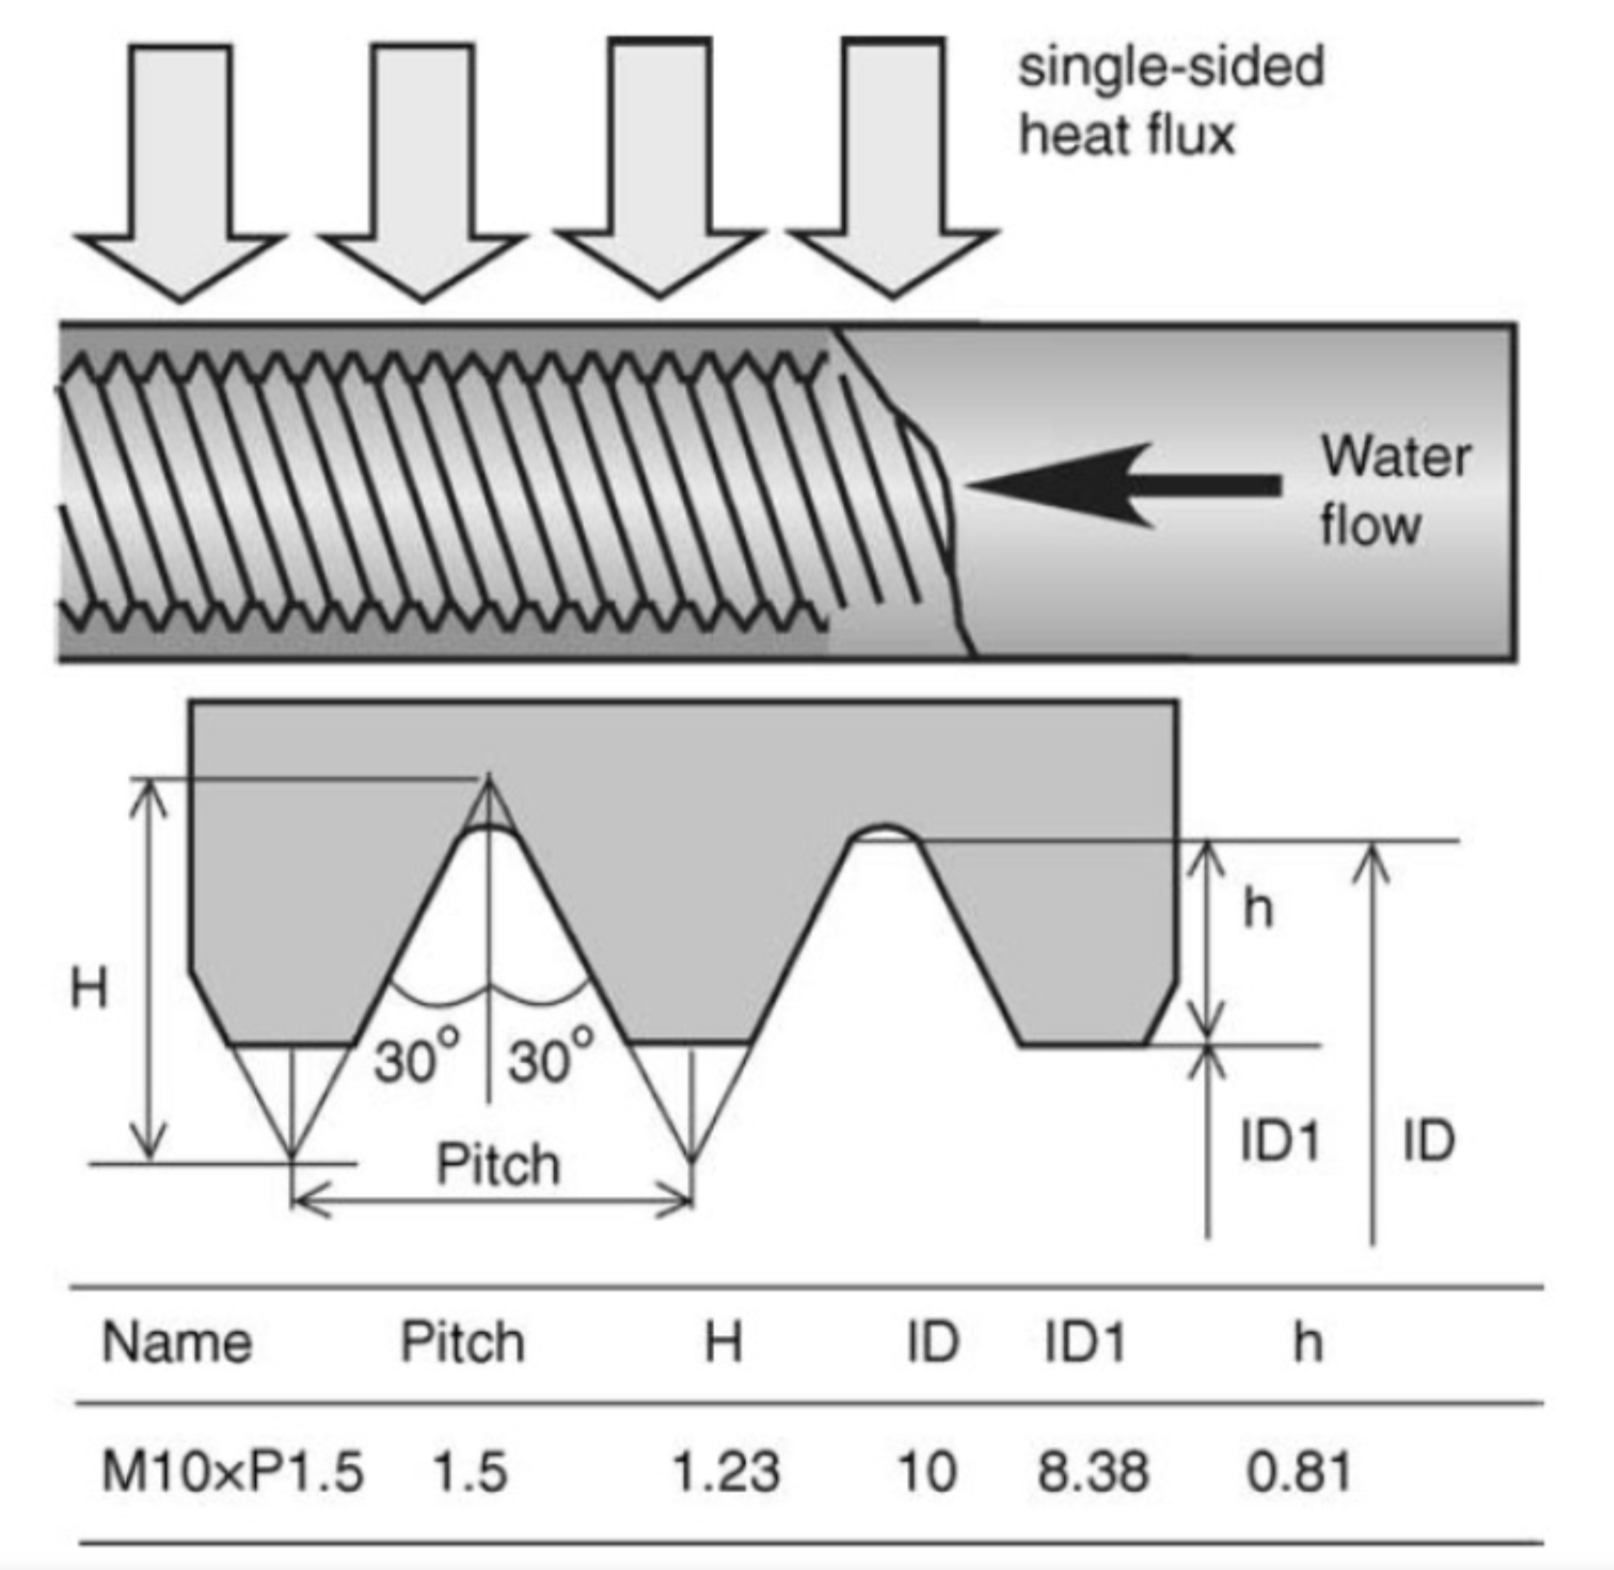
\includegraphics[width=\linewidth]{alternative_HF2.png}
      \caption{Schematic view of a screw tube and heating condition \cite{Ezato2005}.}
  \end{minipage}
  \label{fig:alternative_cooling}
\end{figure}

\noindent Figure \ref{fig:alternative_cooling}(left) shows the jet impingement cooling is another approach used to increase CHF, particularly effective when targeting curved surfaces. By directing high-velocity jets of water onto a heated surface, localized heat removal can be maximized. For instance, jet impingement has achieved a maximum CHF of 38~MW/m$^2$ under optimized conditions. While planar jet cooling methods can offer compact system designs with minimal pressure drop, jet cooling on curved surfaces proves to be more efficient for distributing high heat loads \cite{Inoue2000}.
Heat pipes, which are passive heat exchangers, offer another effective solution. They require no mechanical pumping and are capable of removing high localized heat fluxes of over 10~MW/m$^2$. Heat pipes are particularly advantageous because they can operate against gravity, control heat removal at constant temperatures, and reduce the risk of fluid leakage \cite{osti_374458}.
\\
\\
\noindent Finally, screw tubes represent a promising fusion cooling channel solution. These tubes shown in Figure \ref{fig:alternative_cooling}(right) feature a helical triangular fin along the inner surface, which promotes turbulence and increases the heat transfer area. Screw tubes have demonstrated the ability to handle heat fluxes exceeding 20~MW/m$^2$, outperforming smooth tubes in several experiments \cite{Ezato2005}.
\\
\\
\noindent Each of these alternative solutions offers unique advantages for managing the extreme heat fluxes encountered in fusion reactors. A related design direction is the use of strongly structured or finned internal channels, including concepts investigated in the GyroSTEAM/STEAM cooling work, where geometry is optimized to increase heat-transfer area while maintaining acceptable structural deformation and hydraulic losses. Porous structures follow the same general design philosophy but extend it to a three-dimensional interconnected network; they are therefore treated separately in Section~\ref{sec:porous_channels}.
Another broad field of alternative solutions for high heat flux cooling are porous media channels and other similar structures (the gyroid model or the triply periodic minimum surfaces), examined in this thesis \cite{Saghir2024}.
\pagebreak
\section{Critical heat flux}
The critical heat flux (CHF) represents the maximum heat flux that a coolant can absorb from a surface before a drastic reduction in heat transfer efficiency occurs \cite{Ciric}. 
Beyond this threshold, the coolant transitions from a boiling regime to a vapor-dominant regime, leading to a significant rise in surface temperature and potential overheating. 
This phenomenon is primarily due to the formation of a vapor layer on the surface, which acts as an insulating barrier, impeding effective heat transfer. In fusion reactors, where extreme thermal loads are common, accurately predicting and managing CHF is vital to prevent overheating of structural components and ensure operational safety. 
Research in this area often employs advanced experimental techniques and computational models to characterize CHF limits and develop cooling strategies that enhance reactor performance and reliability.

\subsection{Nukiyama curve}

The Nukiyama curve is a fundamental concept in thermal hydraulics that describes the relationship between heat flux and surface temperature during boiling processes. 
It characterizes the behavior of a cooling surface subjected to increasing heat fluxes and illustrates the critical transition points in heat transfer performance. 
The curve typically shows three distinct regions: the nucleate boiling regime, the critical heat flux (CHF) point, and the post-CHF regime. 
In the nucleate boiling regime, heat transfer is efficient due to the vigorous formation and collapse of vapor bubbles. 
As the heat flux increases, the curve reaches a peak at the CHF point, where the heat transfer rate begins to decline sharply. 
Beyond this point, the cooling surface experiences a rapid increase in temperature due to the formation of a vapor film that insulates the surface, significantly reducing heat transfer efficiency. 
Understanding the Nukiyama curve is crucial for designing and optimizing cooling systems in high-heat-flux applications, such as nuclear reactors, where managing heat flux and preventing surface overheating are essential for safe and efficient operation. 
The curve provides insights into boiling heat transfer mechanisms and guides the development of advanced cooling strategies to enhance thermal management.
\begin{figure}[h]
  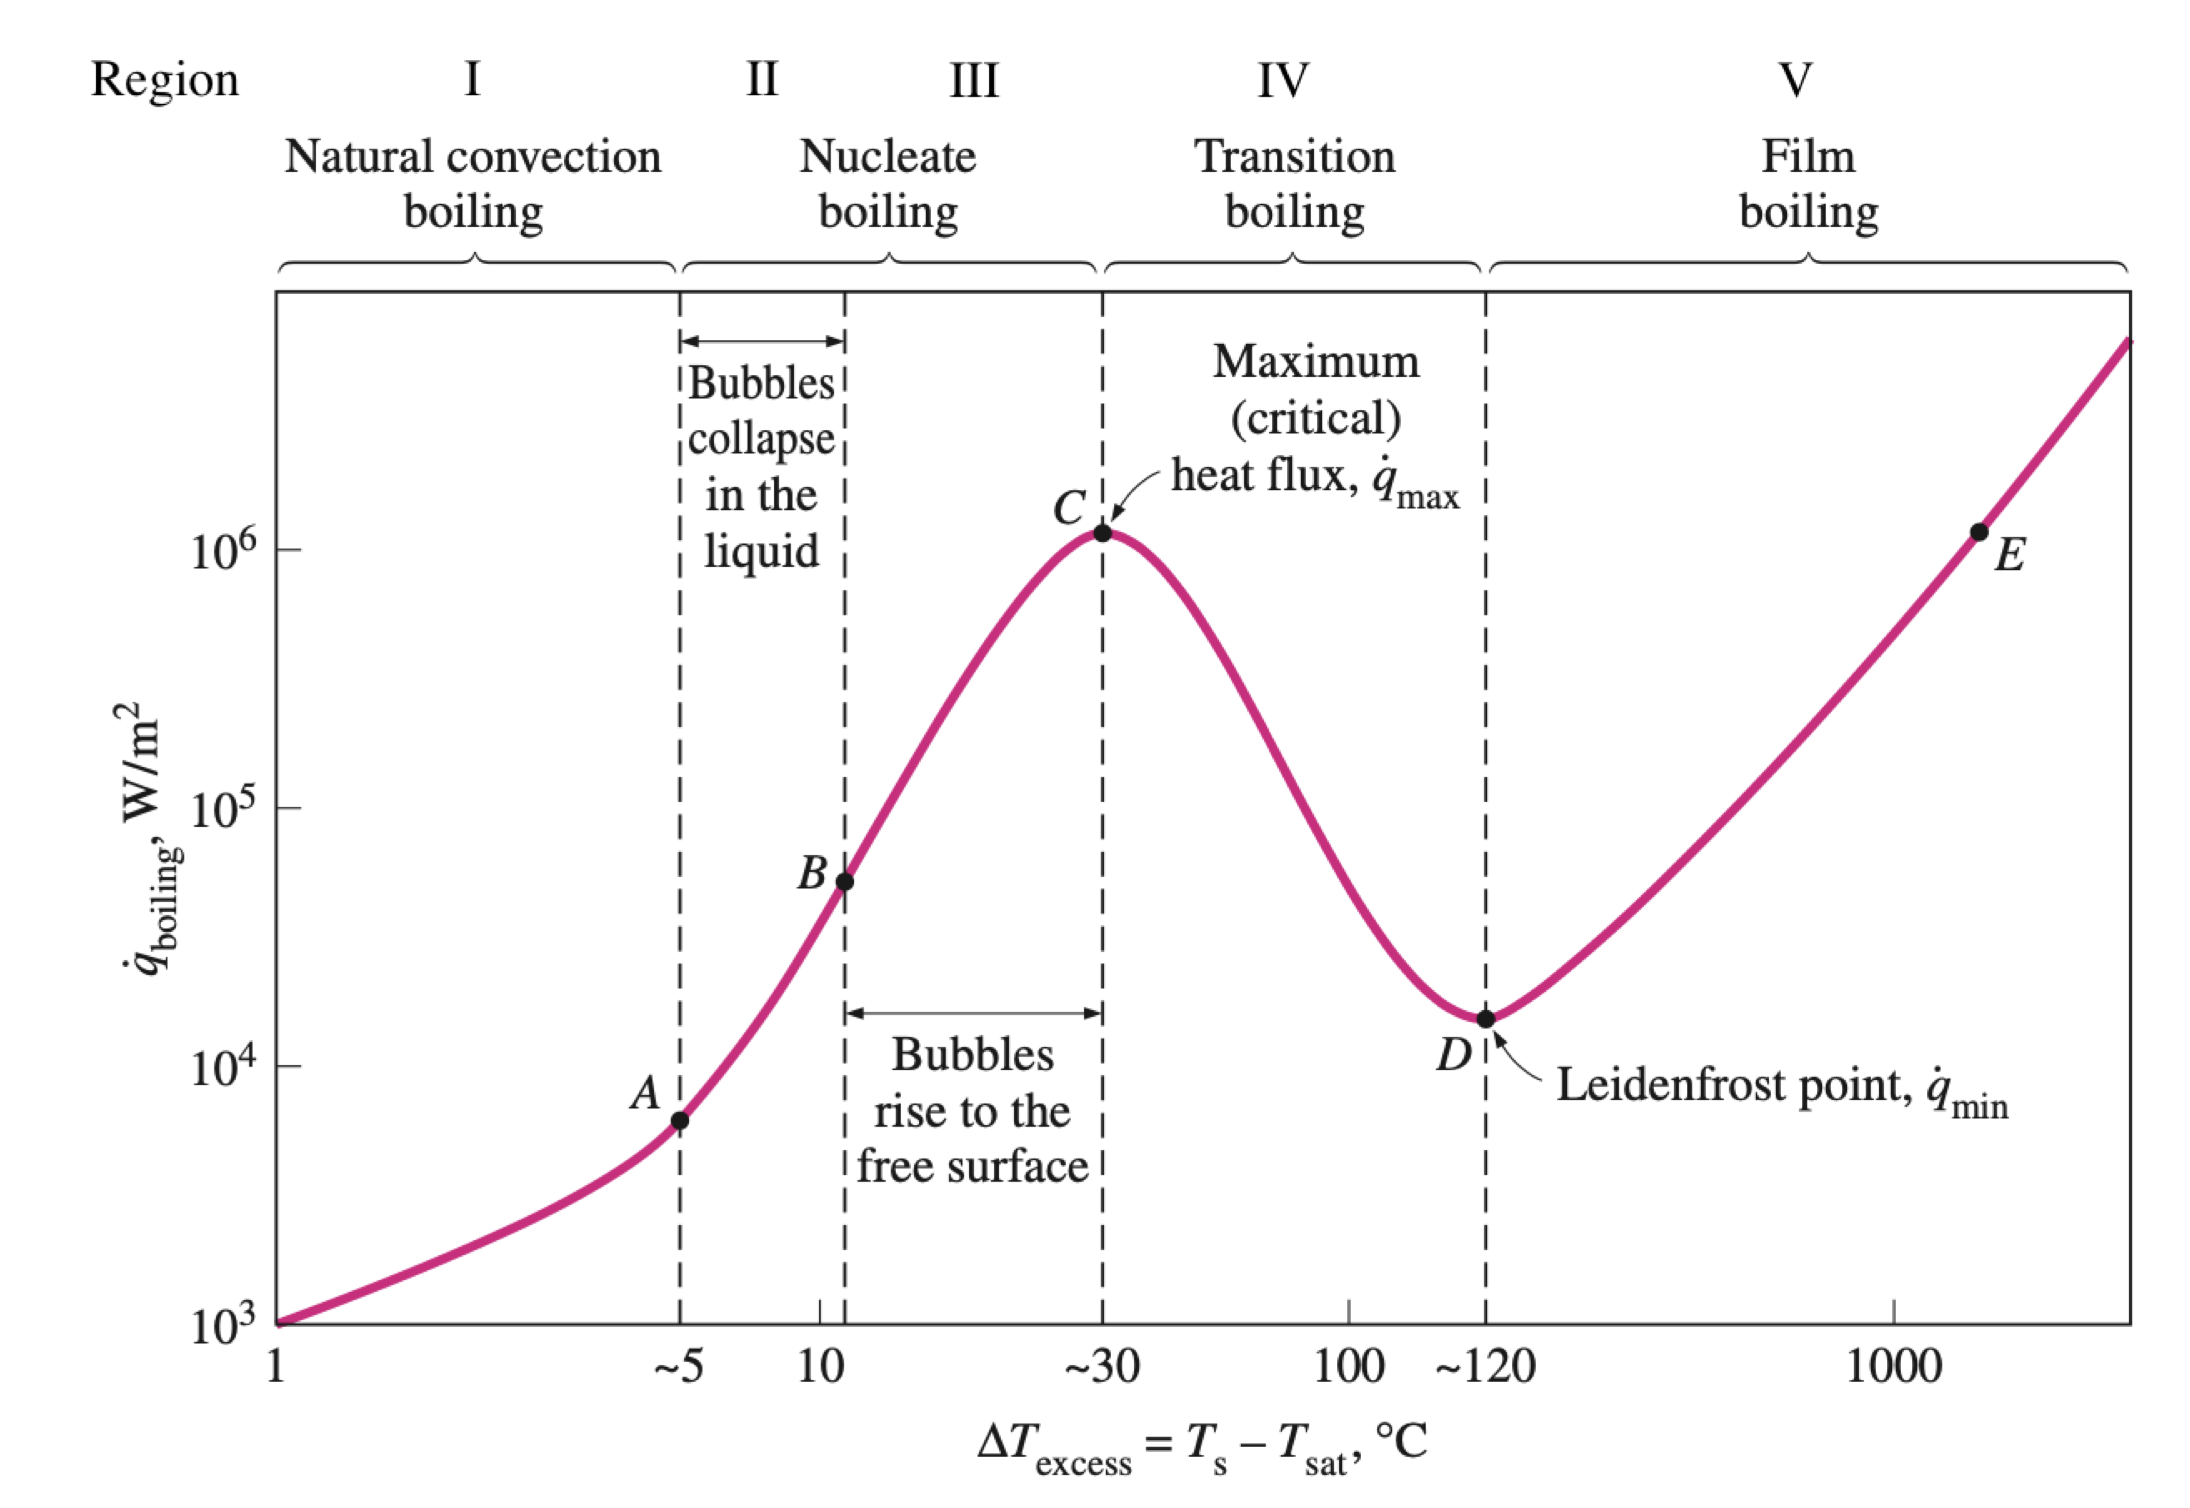
\includegraphics[width=12cm]{nukiyama_ref.png}
  \centering
  \caption{Nukiyama boiling curve \cite{Leong2017-ag}}
  \label{fig:nuk}
\end{figure}

\pagebreak
\section{Porous material based cooling channels}
\label{sec:porous_channels}
Porous material-based cooling channels have emerged as an alternative solution for managing thermal loads in various high-performance applications. 
These channels leverage the unique properties of porous materials, such as high surface area, enhanced fluid mixing, and the capillary effect, to optimize heat transfer and fluid flow. 
By carefully selecting and designing porous material cooling channels, high cooling efficiency and increased critical heat flux can be achieved.
\subsection{An overview of previously conducted research}

\begin{table}[ht!]
\centering
\resizebox{14cm}{10cm}{
  \begin{tabular}{|l|c|c|c|c|c|c|c|c|c|}
  \hline
  \multicolumn{1}{|c|}{\textbf{\rotatebox{90}{Author}} } & \textbf{\rotatebox{90}{Experimental}} & \textbf{\rotatebox{90}{Numerical}} & \textbf{\rotatebox{90}{Pressure Drop}} & \textbf{\rotatebox{90}{Heat Transfer}} & \textbf{\rotatebox{90}{Porosity ($\varphi$)}} & \textbf{\rotatebox{90}{PPI}} & \textbf{\rotatebox{90}{2-Phase}} & \textbf{\rotatebox{90}{Fluid Material}} & \textbf{\rotatebox{90}{Solid Material}} \\
  \hline
  Youchison \cite{Youchison2007} & \cellcolor[HTML]{C0C0C0}\textbf{\textbullet} &  & \cellcolor[HTML]{C0C0C0}\textbf{\textbullet} & \cellcolor[HTML]{C0C0C0}\textbf{\textbullet} & & & & He & W \\
  \hline
  Raffay \cite{Raffray2003} & & \cellcolor[HTML]{C0C0C0}\textbf{\textbullet} & \cellcolor[HTML]{C0C0C0}\textbf{\textbullet} & \cellcolor[HTML]{C0C0C0}\textbf{\textbullet} & 0.5-0.95 & & & He &  \\
  \hline
  Kisitu \cite{Kisitu2022} & \cellcolor[HTML]{C0C0C0}\textbf{\textbullet} &  &\cellcolor[HTML]{C0C0C0}\textbf{\textbullet} &\cellcolor[HTML]{C0C0C0}\textbf{\textbullet}  & 0.62/0.91 & 40& \cellcolor[HTML]{C0C0C0}\textbf{\textbullet} & R134a & Cu\\
  \hline
  Diani \cite{Diani2014} & \cellcolor[HTML]{C0C0C0}\textbf{\textbullet} &  &\cellcolor[HTML]{C0C0C0}\textbf{\textbullet} &\cellcolor[HTML]{C0C0C0}\textbf{\textbullet}  & 0.93 & 5 & \cellcolor[HTML]{C0C0C0}\textbf{\textbullet} & R134a & Cu\\
  \hline
  Li \cite{Li2019} & \cellcolor[HTML]{C0C0C0}\textbf{\textbullet} &  & &\cellcolor[HTML]{C0C0C0}\textbf{\textbullet}  & 0.98 & 110 & \cellcolor[HTML]{C0C0C0}\textbf{\textbullet} & R141b & Cu\\
  \hline
  Athreya \cite{Athreya2002} & \cellcolor[HTML]{C0C0C0}\textbf{\textbullet} &  & &\cellcolor[HTML]{C0C0C0}\textbf{\textbullet}  & 0.89-0.98 & 5-18 & \cellcolor[HTML]{C0C0C0}\textbf{\textbullet} & FC-72 & Al\\
  \hline
  El-Genk \cite{ElGenk2012} & \cellcolor[HTML]{C0C0C0}\textbf{\textbullet} &  & &\cellcolor[HTML]{C0C0C0}\textbf{\textbullet}  & 0.61 &  & \cellcolor[HTML]{C0C0C0}\textbf{\textbullet} & FC-72/HFE-7100 & C \\
  \hline
  Thiagarajan \cite{Thiagarajan2015} & \cellcolor[HTML]{C0C0C0}\textbf{\textbullet} &  & &\cellcolor[HTML]{C0C0C0}\textbf{\textbullet}  & 0.55-0.6 &  & \cellcolor[HTML]{C0C0C0}\textbf{\textbullet} & HFE-7100 & Cu \\
  \hline
  Cen \cite{Cen2023} & \cellcolor[HTML]{C0C0C0}\textbf{\textbullet} &  & &\cellcolor[HTML]{C0C0C0}\textbf{\textbullet}  & 0.825 & 31.75 & \cellcolor[HTML]{C0C0C0}\textbf{\textbullet} & HFE-7100 & Cu \\
  \hline
  Mancin \cite{Mancin2013}& \cellcolor[HTML]{C0C0C0}\textbf{\textbullet} &  & & & 0.896-0.956 & 5-40 & & Air & Cu  \\
  \hline
  Mancin \cite{Mancin2012}& \cellcolor[HTML]{C0C0C0}\textbf{\textbullet} &  & \cellcolor[HTML]{C0C0C0}\textbf{\textbullet}  & \cellcolor[HTML]{C0C0C0}\textbf{\textbullet} & 0.905-0.934 & 5-40 & & Air & Cu  \\
  \hline
  Zafari \cite{Zafari2015}&   & \cellcolor[HTML]{C0C0C0}\textbf{\textbullet}  & \cellcolor[HTML]{C0C0C0}\textbf{\textbullet} & \cellcolor[HTML]{C0C0C0}\textbf{\textbullet} & 0.85-0.95& & & Air & Al/Cu \\
  \hline
  Liu \cite{Liu2017}&  &  & \cellcolor[HTML]{C0C0C0}\textbf{\textbullet} &\cellcolor[HTML]{C0C0C0}\textbf{\textbullet}  & 0.9-0.91& 10& & Air & Al \\
  \hline
  Iasello \cite{Iasiello2017}&  & \cellcolor[HTML]{C0C0C0}\textbf{\textbullet}  & & \cellcolor[HTML]{C0C0C0}\textbf{\textbullet} & 0.87-0.94 & 5-40 & & Air & Al  \\
  \hline
  Younis \cite{Younis1993}& \cellcolor[HTML]{C0C0C0}\textbf{\textbullet} &   & & \cellcolor[HTML]{C0C0C0}\textbf{\textbullet} & 0.834-0.87 & 4-26 & & Air & Al  \\
  \hline
  Dukhan \cite{Dukhan2006}& \cellcolor[HTML]{C0C0C0}\textbf{\textbullet} &   & \cellcolor[HTML]{C0C0C0}\textbf{\textbullet}&  & 0.679-0.924 & 10-40 & & Air & Al  \\
  \hline
  Vijay \cite{Vijay2015}& \cellcolor[HTML]{C0C0C0}\textbf{\textbullet} & \cellcolor[HTML]{C0C0C0}\textbf{\textbullet}  & \cellcolor[HTML]{C0C0C0}\textbf{\textbullet}& \cellcolor[HTML]{C0C0C0}\textbf{\textbullet} & 0.79-0.87 & 10-30 & & Air & Al  \\
  \hline
  Ranut \cite{Ranut2015} &  & \cellcolor[HTML]{C0C0C0}\textbf{\textbullet}  & \cellcolor[HTML]{C0C0C0}\textbf{\textbullet} & \cellcolor[HTML]{C0C0C0}\textbf{\textbullet} & 0.94 & 10-30 & & Air & Al \\
  \hline
  Bilen \cite{Bilen2017}& \cellcolor[HTML]{C0C0C0}\textbf{\textbullet} &  & & \cellcolor[HTML]{C0C0C0}\textbf{\textbullet} & 0.92 & 40 &  & Air & Al \\
  \hline
  Bhaskar \cite{Bhaskar2017}& \cellcolor[HTML]{C0C0C0}\textbf{\textbullet} &  & \cellcolor[HTML]{C0C0C0}\textbf{\textbullet} & \cellcolor[HTML]{C0C0C0}\textbf{\textbullet} & 0.9 & 20 &  & Air & Al \\
  \hline
  Calmidi \cite{Calmidi2000}& \cellcolor[HTML]{C0C0C0}\textbf{\textbullet} & \cellcolor[HTML]{C0C0C0}\textbf{\textbullet}  & \cellcolor[HTML]{C0C0C0}\textbf{\textbullet} & \cellcolor[HTML]{C0C0C0}\textbf{\textbullet} & 0.9-0.97 & 5-40 &  & Air & Al \\
  \hline
  Mustapha \cite{Mustapha2022}& \cellcolor[HTML]{C0C0C0}\textbf{\textbullet} &  & \cellcolor[HTML]{C0C0C0}\textbf{\textbullet} & & 0.88-0.94 & 10/20 & & Air &  \\
  \hline
  Nowak \cite{Nowak2016}&  & \cellcolor[HTML]{C0C0C0}\textbf{\textbullet}  &\cellcolor[HTML]{C0C0C0}\textbf{\textbullet}  & & & & & Air &  \\
  \hline
  Zhang \cite{Zhang2020} & \cellcolor[HTML]{C0C0C0}\textbf{\textbullet}  & \cellcolor[HTML]{C0C0C0}\textbf{\textbullet}  & \cellcolor[HTML]{C0C0C0}\textbf{\textbullet}  & & 0.8-0.92& 15-45 & & Air & Ni \\
  \hline
  Kang \cite{Kang2019} &  \cellcolor[HTML]{C0C0C0}\textbf{\textbullet} &\cellcolor[HTML]{C0C0C0}\textbf{\textbullet} & & \cellcolor[HTML]{C0C0C0}\textbf{\textbullet}& 0.9& & & Air& Si \\
  \hline
  Gorgun \cite{Gorgun2020}&  & \cellcolor[HTML]{C0C0C0}\textbf{\textbullet}  & \cellcolor[HTML]{C0C0C0}\textbf{\textbullet} &  & 0.364& & & Air & Co/Ni/Fe \\
  \hline
  Jiang, Li \cite{Jiang2004} & \cellcolor[HTML]{C0C0C0}\textbf{\textbullet}  &  & \cellcolor[HTML]{C0C0C0}\textbf{\textbullet}& \cellcolor[HTML]{C0C0C0}\textbf{\textbullet}& 0.402-0.486& & & Water/Air& Cu/Bronze \\
  \hline
  Bhattarchya \cite{Bhattacharya2002}& \cellcolor[HTML]{C0C0C0}\textbf{\textbullet} &  & & \cellcolor[HTML]{C0C0C0}\textbf{\textbullet} & 0.9-0.97 & 5-40 & &Water/Air & Al  \\
  \hline
  Abadi \cite{BamorovatAbadi2016}& \cellcolor[HTML]{C0C0C0}\textbf{\textbullet} &  & \cellcolor[HTML]{C0C0C0}\textbf{\textbullet} & \cellcolor[HTML]{C0C0C0}\textbf{\textbullet} & 0.96&30-60 & & Water/R235fa &  Cu \\
  \hline
  Kibushi \cite{Kibushi2021}& \cellcolor[HTML]{C0C0C0}\textbf{\textbullet} &  &  & \cellcolor[HTML]{C0C0C0}\textbf{\textbullet} & 0.659& & \cellcolor[HTML]{C0C0C0}\textbf{\textbullet}& Water/FC-72 &  Cu \\
  \hline
  Moghaddam \cite{Moghaddam2003}& \cellcolor[HTML]{C0C0C0}\textbf{\textbullet} &  &  & \cellcolor[HTML]{C0C0C0}\textbf{\textbullet} & 0.9-0.95& 30-80 & \cellcolor[HTML]{C0C0C0}\textbf{\textbullet}& Water/FC-72 &  Cu/C \\
  \hline
  Wang \cite{Wang2018}& \cellcolor[HTML]{C0C0C0}\textbf{\textbullet} &  &  & \cellcolor[HTML]{C0C0C0}\textbf{\textbullet} & 0.98& 40 & & Water &  Cu/Ni \\
  \hline
  Ding \cite{Ding2011}& \cellcolor[HTML]{C0C0C0}\textbf{\textbullet} &  &  & \cellcolor[HTML]{C0C0C0}\textbf{\textbullet} & 0.7-0.9&  & & Water &  Cu \\
  \hline
  Xiao \cite{Xiao2013} & \cellcolor[HTML]{C0C0C0}\textbf{\textbullet}  &  & \cellcolor[HTML]{C0C0C0}\textbf{\textbullet} & \cellcolor[HTML]{C0C0C0}\textbf{\textbullet} & 0.6-0.8& & & Water & Cu \\
  \hline
  Gong \cite{Gong2018}& \cellcolor[HTML]{C0C0C0}\textbf{\textbullet} &  &\cellcolor[HTML]{C0C0C0}\textbf{\textbullet}  & \cellcolor[HTML]{C0C0C0}\textbf{\textbullet} & 0.66 & & & Water & Cu \\
  \hline
  Wang \cite{Wang2023}& \cellcolor[HTML]{C0C0C0}\textbf{\textbullet} &  &  & \cellcolor[HTML]{C0C0C0}\textbf{\textbullet} & 0.96 & 10-90 & & Water & Cu \\
  \hline
  Kim \cite{Kim2014}& \cellcolor[HTML]{C0C0C0}\textbf{\textbullet} &  & \cellcolor[HTML]{C0C0C0}\textbf{\textbullet} & & 0.95-0.98& 10-100 & & Water & Cu  \\
  \hline
  Yuki \cite{Yuki2016}& \cellcolor[HTML]{C0C0C0}\textbf{\textbullet} & & & \cellcolor[HTML]{C0C0C0}\textbf{\textbullet}  & 0.36&  &\cellcolor[HTML]{C0C0C0}\textbf{\textbullet}  & Water & Cu  \\
  \hline
  Ji \cite{Ji2013}& \cellcolor[HTML]{C0C0C0}\textbf{\textbullet} & & & \cellcolor[HTML]{C0C0C0}\textbf{\textbullet}  & 0.95& 30-90 &\cellcolor[HTML]{C0C0C0}\textbf{\textbullet}  & Water & Cu  \\
  \hline
  Fu \cite{Fu2023}& \cellcolor[HTML]{C0C0C0}\textbf{\textbullet} & & \cellcolor[HTML]{C0C0C0}\textbf{\textbullet} & \cellcolor[HTML]{C0C0C0}\textbf{\textbullet}  & 0.78& 110 &\cellcolor[HTML]{C0C0C0}\textbf{\textbullet}  & Water & Cu  \\
  \hline
  Zhang \cite{Zhang2018}& \cellcolor[HTML]{C0C0C0}\textbf{\textbullet} & & & \cellcolor[HTML]{C0C0C0}\textbf{\textbullet}  & 0.33& & & Water & Cu  \\
  \hline
  Hunt \cite{Hunt1988}& \cellcolor[HTML]{C0C0C0}\textbf{\textbullet} &  & \cellcolor[HTML]{C0C0C0}\textbf{\textbullet} & \cellcolor[HTML]{C0C0C0}\textbf{\textbullet} & 0.94-0.97& 4-10 & & Water & C/Ni/Al  \\
  \hline
  Arbak \cite{Arbak2017}& \cellcolor[HTML]{C0C0C0}\textbf{\textbullet} &  & & \cellcolor[HTML]{C0C0C0}\textbf{\textbullet} & 0.876-0.909 & 10/40& & Water & Al \\
  \hline
  Boomssma \cite{Boomsma2001}&    \cellcolor[HTML]{C0C0C0}\textbf{\textbullet}  && \cellcolor[HTML]{C0C0C0}\textbf{\textbullet} & & 0.5-0.9& 10-40 & & Water & Al \\
  \hline
  Manetti \cite{Manetti2020}& \cellcolor[HTML]{C0C0C0}\textbf{\textbullet} &  &  & \cellcolor[HTML]{C0C0C0}\textbf{\textbullet} & 0.9 &  & \cellcolor[HTML]{C0C0C0}\textbf{\textbullet}& HFE-71000 & Cu \\
  \hline
  Xu \cite{Xu2008}& \cellcolor[HTML]{C0C0C0}\textbf{\textbullet} &  &  & \cellcolor[HTML]{C0C0C0}\textbf{\textbullet} & 0.88-0.95 & 30-90 & \cellcolor[HTML]{C0C0C0}\textbf{\textbullet}& Acetone & Cu \\
  \hline
  Yang \cite{Yang2014}&  & \cellcolor[HTML]{C0C0C0}\textbf{\textbullet} & \cellcolor[HTML]{C0C0C0}\textbf{\textbullet}& & 0.55-0.98&5-100 & & &  \\
  \hline
  Du Plesis \cite{DuPlessis1994} & \cellcolor[HTML]{C0C0C0}\textbf{\textbullet} &  & \cellcolor[HTML]{C0C0C0}\textbf{\textbullet}  & & 0.973-0.978& & & Glycerol $\odot$  &  \\
  \hline
  Sinn \cite{Sinn2019} &  &  & \cellcolor[HTML]{C0C0C0}\textbf{\textbullet}  & \cellcolor[HTML]{C0C0C0}\textbf{\textbullet} & 0.77 & 10 &  & CO$_2$  & Al/s-SicC/mullite  \\
  \hline
  \end{tabular} 
}
\caption{An Overview of Porous Material Research}
\label{table:prehled_pen}
\end{table}


\noindent Table \ref{table:prehled_pen} shows and overview of previously conducted research of cooling channels based on porous materials.
Numerous studies have focused on experimental investigations, providing valuable insights into the real-world performance of porous material-based cooling channels. For instance, Youchison \cite{Youchison2007}, Kisitu \cite{Kisitu2022}, and Diani \cite{Diani2014} have all conducted experimental studies that primarily addressed pressure drop and heat transfer characteristics. 
These studies often involve the use of various porous materials and fluids to understand how different configurations affect cooling performance.
On the numerical side, Raffray \cite{Raffray2003}, Zafari \cite{Zafari2015}, and Vijay \cite{Vijay2015} contributed significantly to the theoretical understanding of these systems. 
Numerical studies allow the simulation of various scenarios that may be challenging to replicate experimentally, offering predictions on the behavior of porous media in different cooling applications.
There are various numerical approaches to solve the porous media domain applied in the mentioned literature overview such as ANSYS CFX \cite{Ranut2015,Gong2018},ANSYS Fluent, \cite{Nowak2016,Zhang2020}, COMSOL \cite{Iasiello2017}, MERLOT \cite{Raffray2003} or their own code \cite{Kang2019,Vijay2015}.

\begin{figure}[h]
  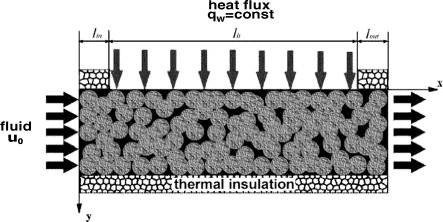
\includegraphics[width=9cm]{exp_set.jpg}
  \centering
  \caption{Schematic of a typical experimental setup \cite{Jiang2004}.
  }
  \label{fig:exp_set}
\end{figure}

\noindent Porosity values in the studies reviewed range widely, from as low as 0.33 in Zhang's study \cite{Zhang2018} to as high as 0.98 in Li's study \cite{Li2019}. Higher porosity generally implies lower material density, which can lead to reduced pressure drops but may also affect the structural integrity and heat transfer performance.
PPI is another critical parameter that defines the pore size and distribution within the porous medium. Studies such as those by Kisitu \cite{Kisitu2022}, Mancin \cite{Mancin2012}, and Bhattarchya \cite{Bhattacharya2002} have investigated materials with varying PPI values, showing how different PPI values influence the overall performance of the cooling channels. A higher PPI generally leads to a larger surface area for heat exchange but can also increase the flow resistance, affecting the pressure drop.
\\
\\
\noindent The choice of fluid and solid materials is crucial in designing effective cooling channels. Various fluids have been tested across the reviewed studies, including air, water, refrigerants (e.g., R134a, R141b), and specialty fluids like FC-72 and HFE-7100. The choice of fluid significantly impacts the cooling efficiency and is often chosen based on the specific application and desired thermal properties.
Solid materials used in the porous structures also vary, with common choices including aluminum (Al), copper (Cu), and carbon (C). Studies like those by Gong \cite{Gong2018} and Hunt \cite{Hunt1988} demonstrate the use of copper and carbon, respectively, due to their high thermal conductivity, which enhances heat transfer. Other materials like nickel (Ni), silicon (Si), and composites have also been explored to cater to specific cooling requirements.
Some studies have extended the investigation to two-phase flow systems, where the fluid undergoes a phase change during the cooling process. This can significantly enhance the heat transfer due to latent heat but also complicates the system due to the dynamics of phase change. Kisitu \cite{Kisitu2022} and Kibushi \cite{Kibushi2021} are examples of studies that have delved into two-phase flow systems, highlighting both the potential benefits and challenges of implementing such systems in porous media.


\pagebreak

\subsection{Properties of porous materials}
An overview of the elementary properties and terminology of porous material research is provided.
It is important to note that although there are multiple qualities defined, two materials defined by the same measure can have a completely different microstructure and thus vary in the thermohydraulic properties.
A detailed microscopy analysis is needed to estimate the thermohydraulic behavior of given material.
\subsubsection{Closed vs open cell structure.}
The basic classification of porous materials, which has a major influence on their behaviour in terms of permeability of the flowing fluid through the material.
The definitions of the elementary measures "pore, strut, node and cell" are defined in Figure \ref{fig:openclosed}(b).
\begin{figure}[h]
  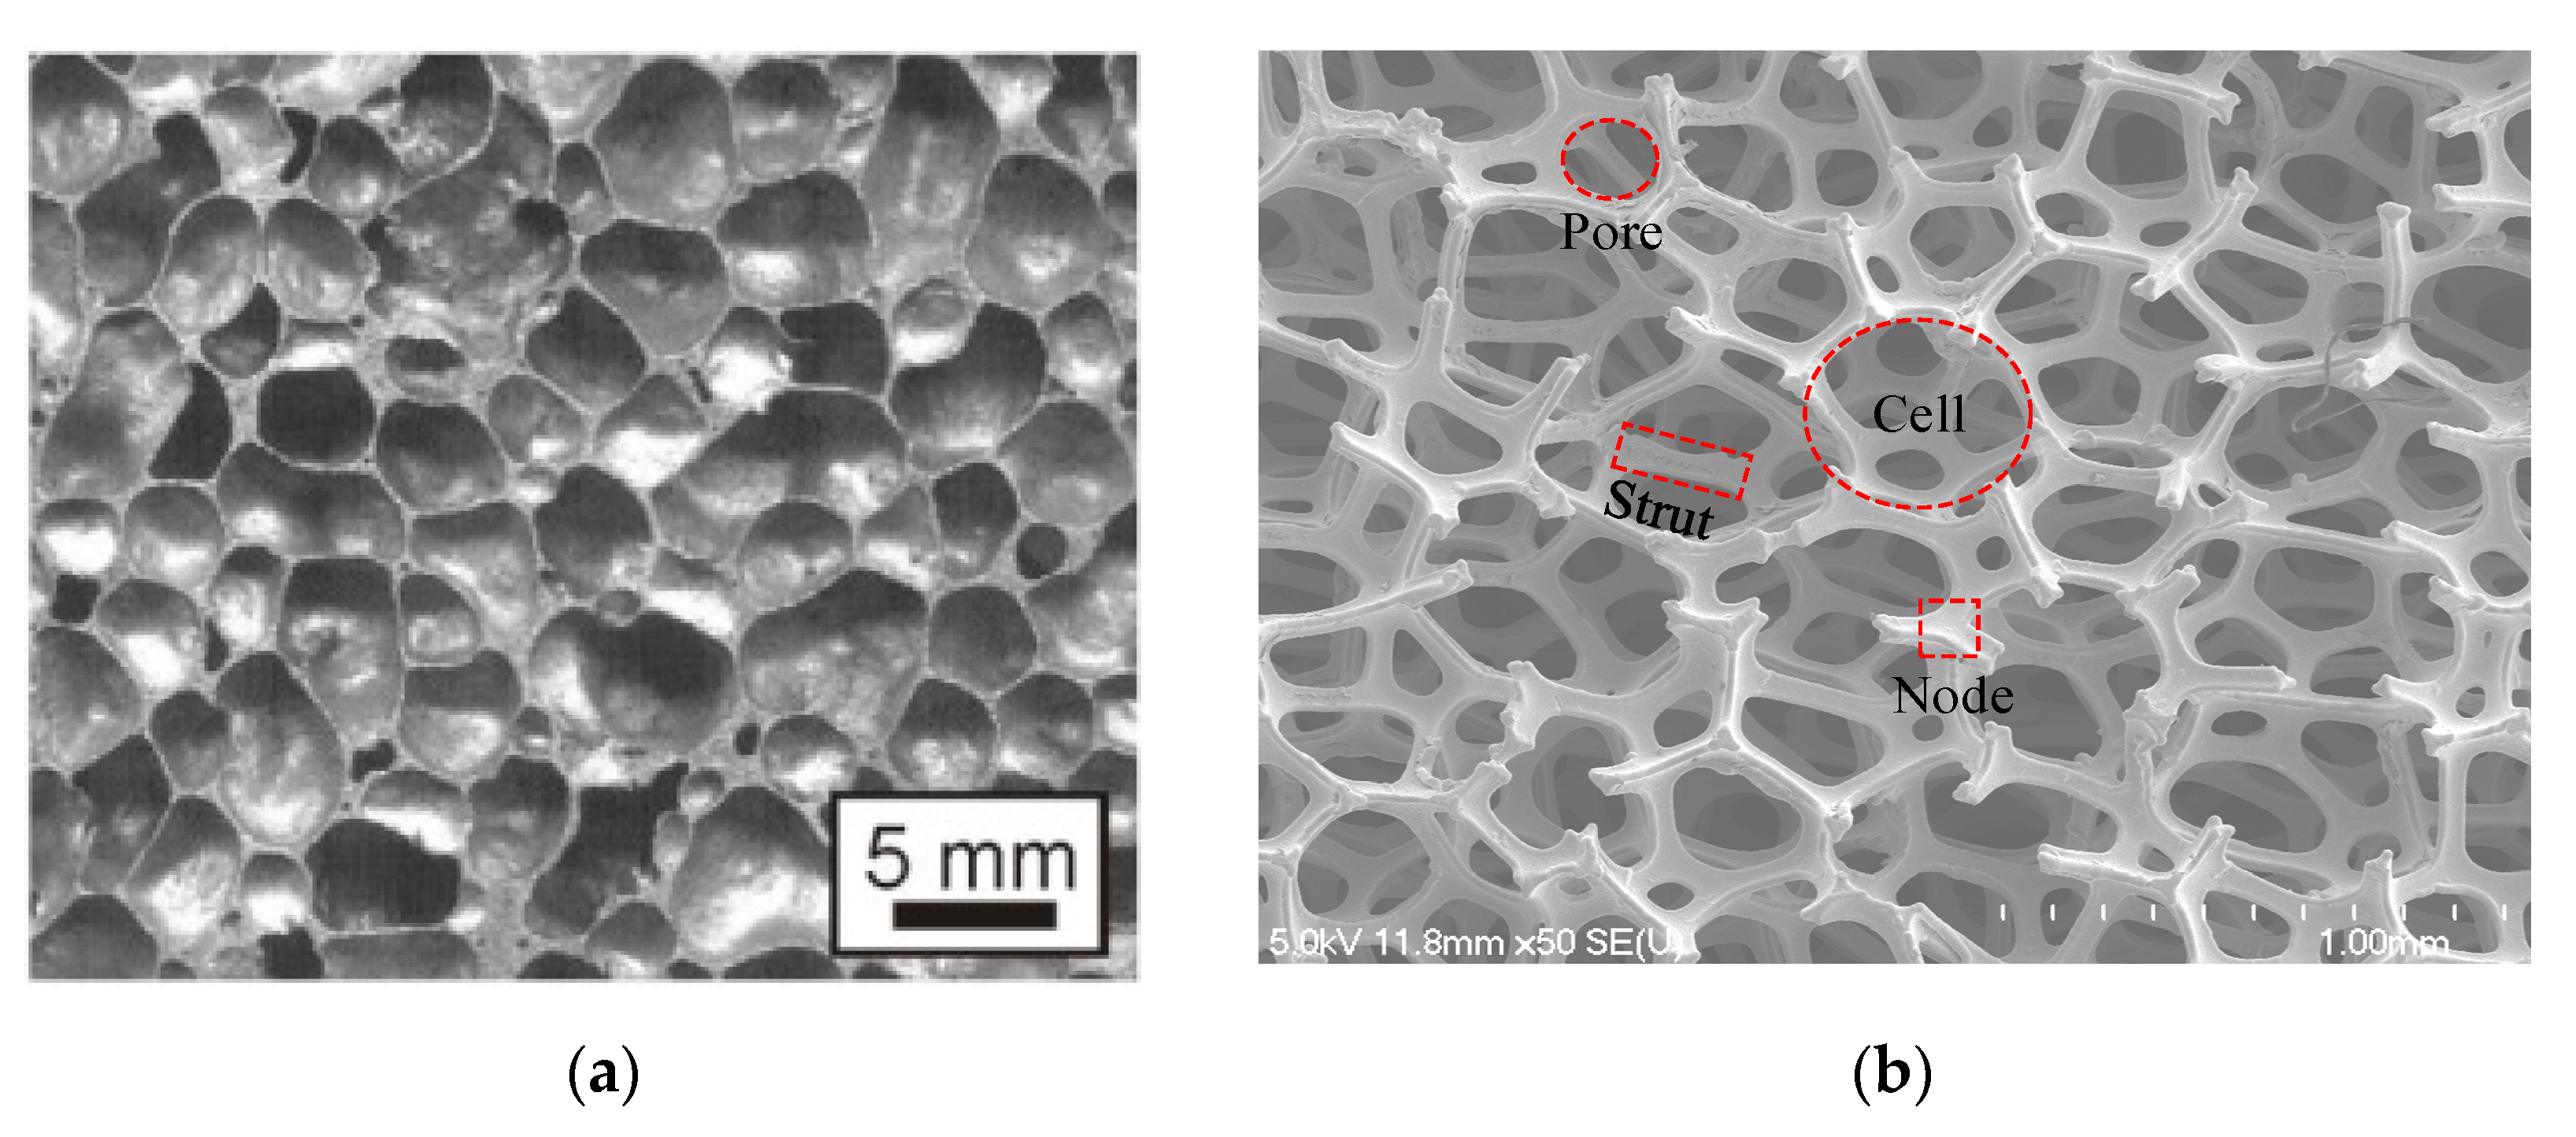
\includegraphics[width=12cm]{open_closed.png}
  \centering
  \caption{Closed (a) vs open (b) cell structure \cite{Yang2021}.
  }
  \label{fig:openclosed}
\end{figure}

\subsubsection{Porosity}
Porosity ($\Phi$) is a fundamental property of porous materials, defined as the ratio of the volume of voids or pores ($V_p$) within a material to the total bulk volume ($V_t$) of the material, including both the solid and void components. 
Porosity can be expressed as: 

\begin{equation}
  \Phi = \dfrac{V_p}{V_t}
\end{equation}

\noindent Porosity is typically expressed as a dimensionless fraction (ranging from 0 to 1) or as a percentage. 
In porous structures, the porosity is a critical parameter that influences various physical properties such as permeability, fluid retention, and mechanical strength. 
High porosity indicates that the material has a large proportion of void space, which can enhance properties like fluid flow or gas diffusion but may reduce mechanical strength. 
Conversely, low porosity suggests a denser structure with fewer voids, typically resulting in higher mechanical strength and lower permeability.
\pagebreak
\subsubsection{PPI}
PPI, or "pores per inch," is a measure used to quantify the density of pores within a porous material. Specifically, PPI indicates the number of pores that occur within a linear inch of the material. This measurement provides insight into the pore size and distribution within the structure.
PPI can be expressed as:

\begin{equation}
  PPI = \dfrac{\text{Number of pores}}{\text{Length of the material (in inches)}}
\end{equation}
 
\noindent In porous materials, a higher PPI value signifies a greater number of smaller pores per inch, leading to a finer structure. Conversely, a lower PPI value indicates fewer, larger pores, resulting in a coarser structure.
PPI is a critical parameter in applications such as filtration, where the pore size distribution impacts the material's ability to filter particles, and in acoustic insulation, where it affects sound absorption properties. The PPI value is often used alongside porosity to fully characterize the microstructure of porous materials in various scientific and engineering contexts.
An example of materials with variable PPI dimensions are shown in Figure Figure \ref{fig:ppi}.

\begin{figure}[h]
  \centering
  \begin{minipage}{0.6\textwidth}
      \centering
      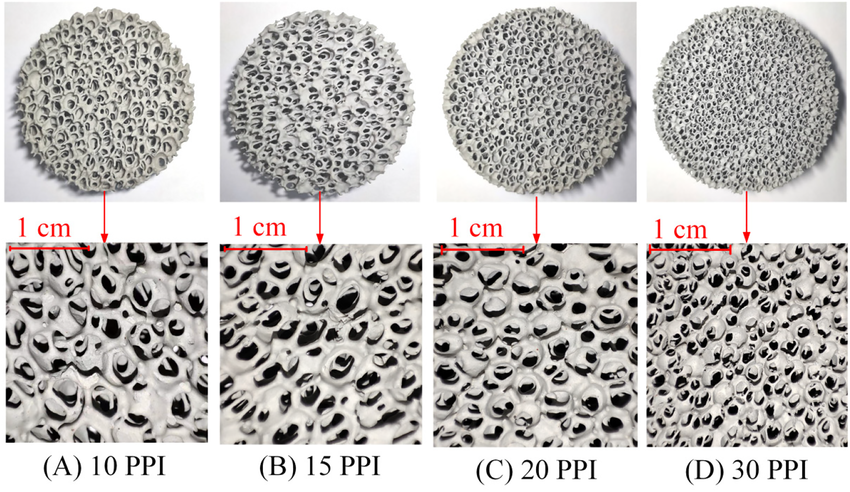
\includegraphics[height=5cm]{ppi_.png}
      \caption{An example of various PPI materials \cite{Chen2021}.}
      \label{fig:ppi}
  \end{minipage}\hfill
  \begin{minipage}{0.4\textwidth}
      \centering
      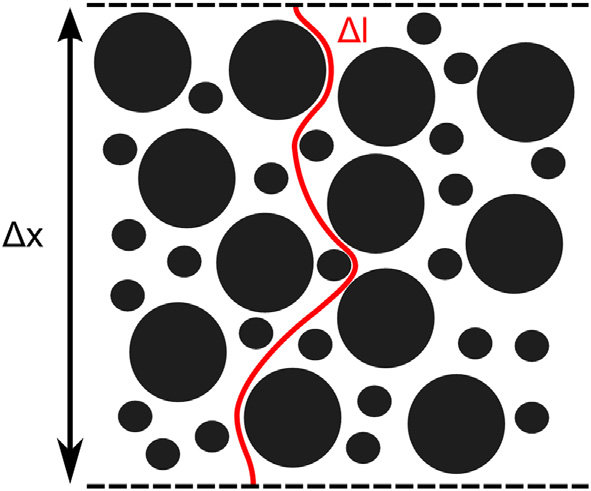
\includegraphics[height=4cm]{tortuosity.png}
      \caption{A 2D illustration of a tortuous path through a porous network \cite{Cooper2014}.}
      \label{fig:tort}
  \end{minipage}
\end{figure}


\subsubsection{Tortuosity}
Tortuosity ($ \tau $) is a key parameter used to describe the complexity of the pathways through the pores in a porous material. 
It represents the degree to which the actual path that a fluid or gas must follow through the porous structure deviates from a straight line. 
In other words, tortuosity quantifies how convoluted or winding the internal pore channels are.
Mathematically, tortuosity can be defined as the ratio of the actual path length ($\Delta l$)that a fluid must travel through the porous medium to the straight-line distance ($\Delta x$) between the inlet and outlet of the porous material.
Figure \ref{fig:tort} represents the mentioned values in a 2D plot.

\begin{equation}
  \tau = \dfrac{\Delta l}{\Delta x} 
\end{equation}

\noindent Tortuosity is always greater than or equal to 1, with a value of 1 indicating a perfectly straight path (no deviation) and higher values indicating more complex, winding pathways.
Tortuosity is a critical factor in determining the transport properties of porous materials, such as diffusivity, permeability, and conductivity. A higher tortuosity implies more resistance to fluid flow and slower diffusion rates, as the fluid must navigate more complex paths. 
This parameter is also affecting the pressure drop in flow through porous material. 

\pagebreak
\subsection{Porous materials manufacturing process}
While metallic foam production methods have existed since the 1950s, their practical use was historically limited due to high production costs and challenging processing factors. However, technological breakthroughs in the 1990s, particularly from Japan's Shinko Wire, led to innovations that significantly improved production efficiency and broadened commercial applications. 
The production of metallic foams now relies on advanced manufacturing techniques, where the process is tailored based on the desired pore structure. Open-cell porous structures are typically produced using solid-state or powder metallurgy methods, while closed-cell foams are created through liquid or melt-based methods. 
Depending on the state of the metal being processed, production routes can be classified into four categories: 
\begin{itemize}
  \item liquid state (melt route)
  \item solid state (powder metallurgy route)
  \item metal vapor
  \item metal ion solution
\end{itemize}

\noindent Schematic shown in Figure \ref{fig:metallic_foam_production} shows how variable can the resulting porous structure be in relation to the manufacturing technology.
Experimental research in the following parts of this thesis is performed on a set of porous foam samples ordered from an external manufacturer, thus the exact manufacturing process is not provided and microscopy analysis of used samples is needed.

\begin{figure}[ht]
  \centering
  \begin{tikzpicture}[scale=0.9]
  % Define the coordinates of the upper blocks
  \node[draw, rectangle, minimum width=3cm, minimum height=1cm, align=center] (block1) at (0, 4) {Liquid metallurgy};
  \node[draw, rectangle, minimum width=3cm, minimum height=1cm, align=center] (block2) at (4, 4) {Ion solution};
  \node[draw, rectangle, minimum width=3cm, minimum height=1cm, align=center] (block3) at (8, 4) {Vapor deposition};
  \node[draw, rectangle, minimum width=3cm, minimum height=1cm, align=center] (block4) at (12, 4) {Powder metallurgy};
  
  % Define the coordinates of the lower blocks (for image placeholders)
  \node[draw, rectangle, minimum width=3cm, minimum height=3cm, align=center] (img1) at (0, 0) {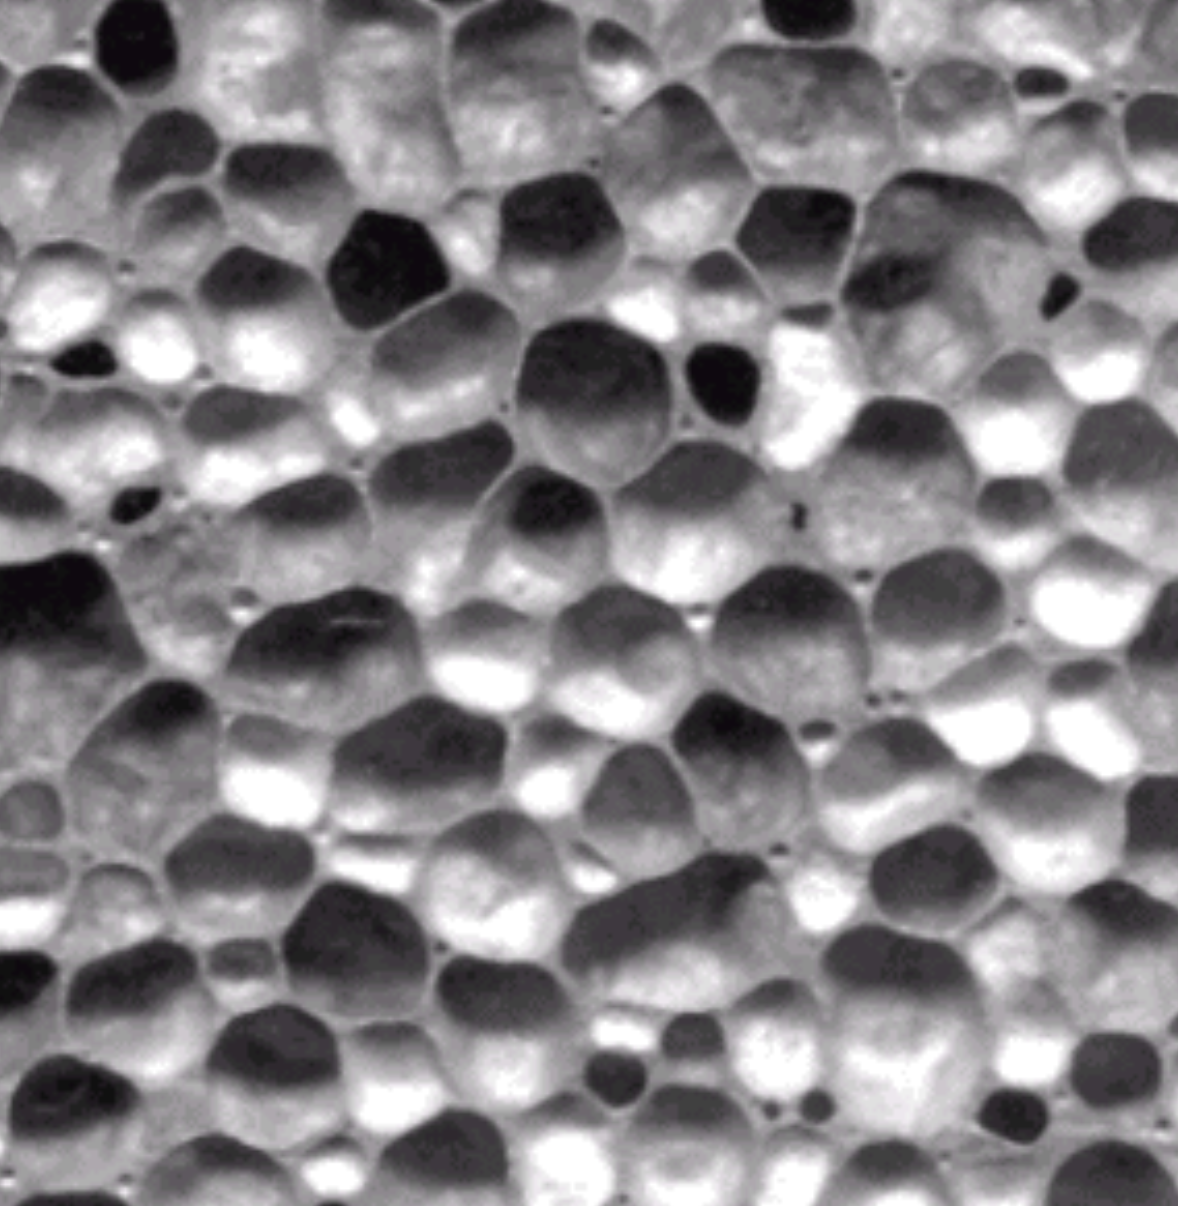
\includegraphics[width=3cm, height=3cm, clip]{structure_2.png}};
  \node[draw, rectangle, minimum width=3cm, minimum height=3cm, align=center] (img2) at (4, 0) {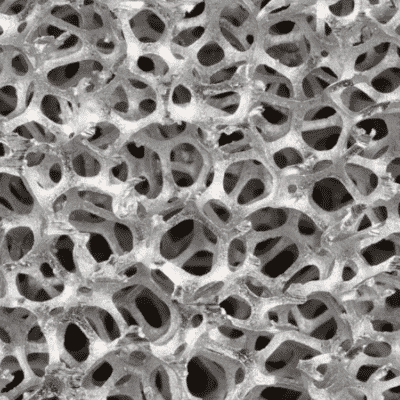
\includegraphics[width=3cm, height=3cm, clip]{structure_1.png}};
  \node[draw, rectangle, minimum width=3cm, minimum height=3cm, align=center] (img3) at (8, 0) {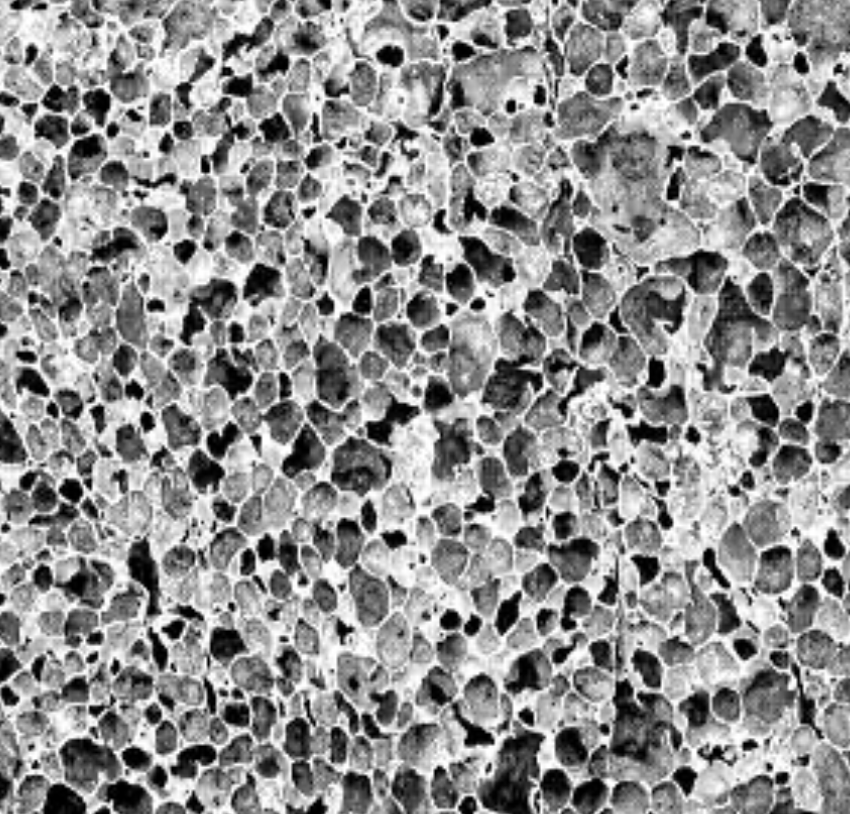
\includegraphics[width=3cm, height=3cm, clip]{structure_3.png}};
  \node[draw, rectangle, minimum width=3cm, minimum height=3cm, align=center] (img4) at (12, 0) {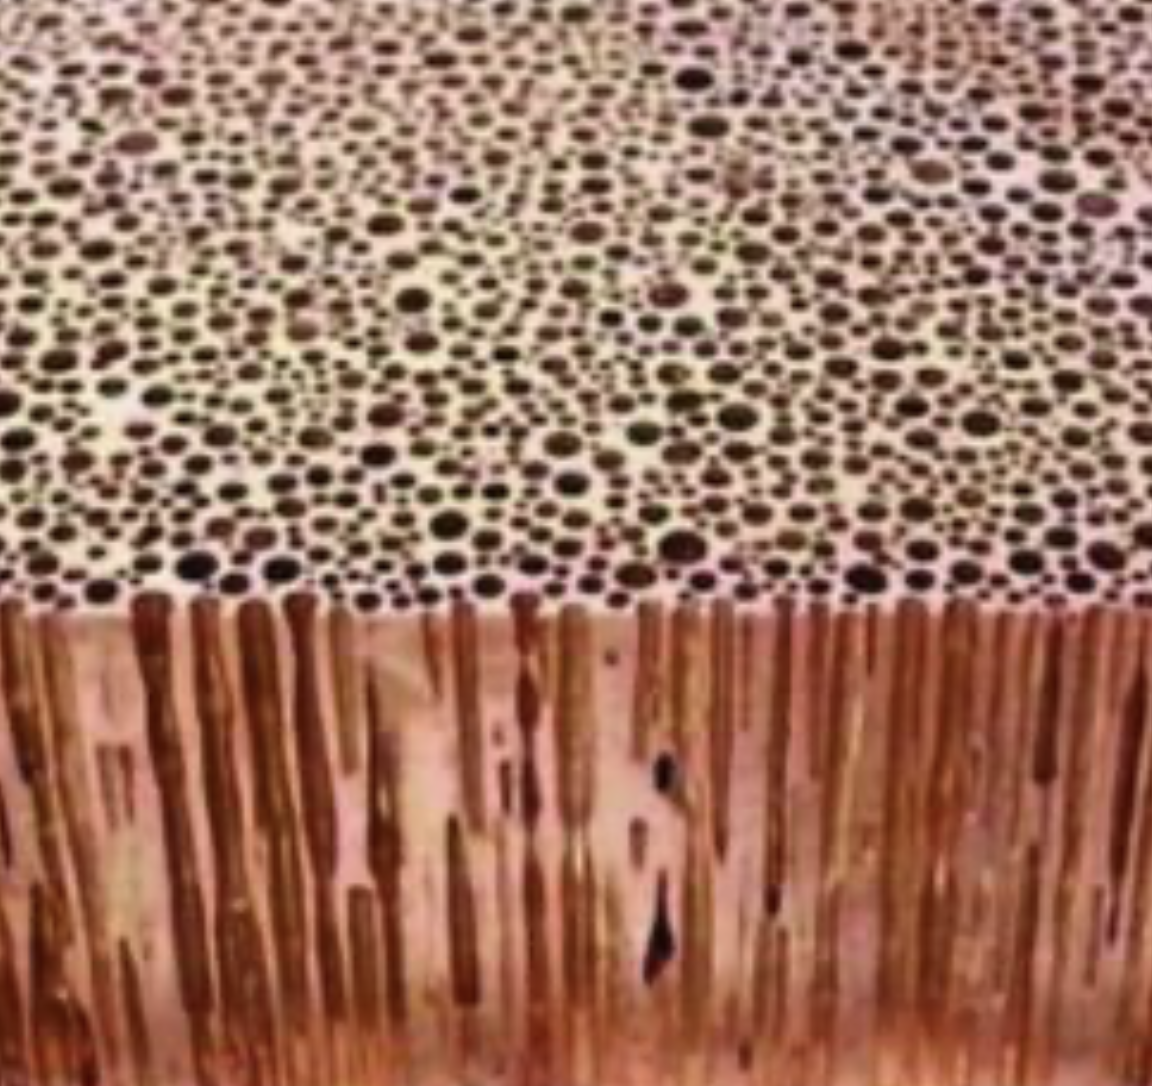
\includegraphics[width=3cm, height=3cm, clip]{structure_4.png}};
  
  % Draw arrow between the first upper block and the third lower block
  \draw[-, thick] (block1.south) -- (img1.north);
  \draw[-, thick] (block1.south) -- (img2.north);
  \draw[-, thick] (block1.south) -- (img4.north);

  \draw[-, thick] (block4.south) -- (img1.north);
  \draw[-, thick] (block4.south) -- (img2.north);
  \draw[-, thick] (block4.south) -- (img3.north);

  \draw[-, thick] (block2.south) -- (img2.north);

  \draw[-, thick] (block3.south) -- (img2.north);

  % Add titles under the image blocks

\node[align=center] at (0, -2.3) {Closed Cell};
\node[align=center] at (4, -2.3) {Open Cell};
\node[align=center] at (8, -2.3) {Partially Open};
\node[align=center] at (12, -2.3) {Lotus Cell};
\end{tikzpicture}
\caption{Different metallic foam production methods with corresponding foam structures.}
\label{fig:metallic_foam_production}
\end{figure}

\subsubsection{Liquid metallurgy}
This method is one of the elementary ways to produce metallic foams, particularly suited for metals and alloys with lower melting points, as the metal is in a liquid state and easier to manage at lower temperatures. 
Metallic foams can be produced with or without the application of pressure.
In the direct foaming method, gas bubbles are introduced into the molten metal either by using a capillary, frit, chemical agents, or by dissolving gas directly in the metal. 
Indirect methods, on the other hand, involve processes like casting liquid metal around solid space-holding filler materials or using polymer foam. These fillers create the pore structure during further processing. 
Another effective method involves melting powder compacts that contain a gas-releasing blowing agent. These various approaches provide flexibility in creating metal foam structures with specific properties.

\pagebreak

\noindent The fabrication of metallic foam via the liquid metallurgy route, initially pioneered and patented during the 1960s and 1970s, experienced a resurgence in scientific activity in the late 1980s, marked by both the revival of traditional methods and the introduction of new techniques. 
Notably, the early 1990s saw Alcan International develop and patent the melt gas injection technique, which is now commercially utilized by Cymat (Canada) and Hydro Aluminum (Norway) for applications in defense, military, architecture, lightweight cores, vibrational dampening, sound attenuation, and marine and offshore sectors. 
This technique involves injecting gas bubbles into molten metal, with the process starting by heating all raw materials to their melting points. Gas is then introduced into the molten metal using nozzles or specially engineered propeller stirrers to ensure a consistent flow and uniform dispersion of bubbles, with CO2, O2, air, nitrogen, argon, or steam being potential gases for injection. 
The gas bubbles, mixed with the molten metal, rise to the surface and solidify to form foam. The size of the bubbles and their distribution in the foam vary depending on the gas pressure and the design of the stirring equipment. The method primarily produces closed-cell metallic foam using inert gases and requires precise control of melt viscosity and temperature to achieve high-quality foam. 
To enhance stability and foam quality, solid stabilizing particles such as Ca, SiC, Si3N4, Al2O3, TiB2, and fly ash are added in small volumes. The foam can undergo two main coarsening mechanisms: disproportionation, where gas pressure differences cause diffusion through cell walls leading to larger average cell size, and coalescence, where bubbles merge to form larger bubbles, potentially causing foam collapse if the coalescence rate is high.

\begin{figure}[h]
  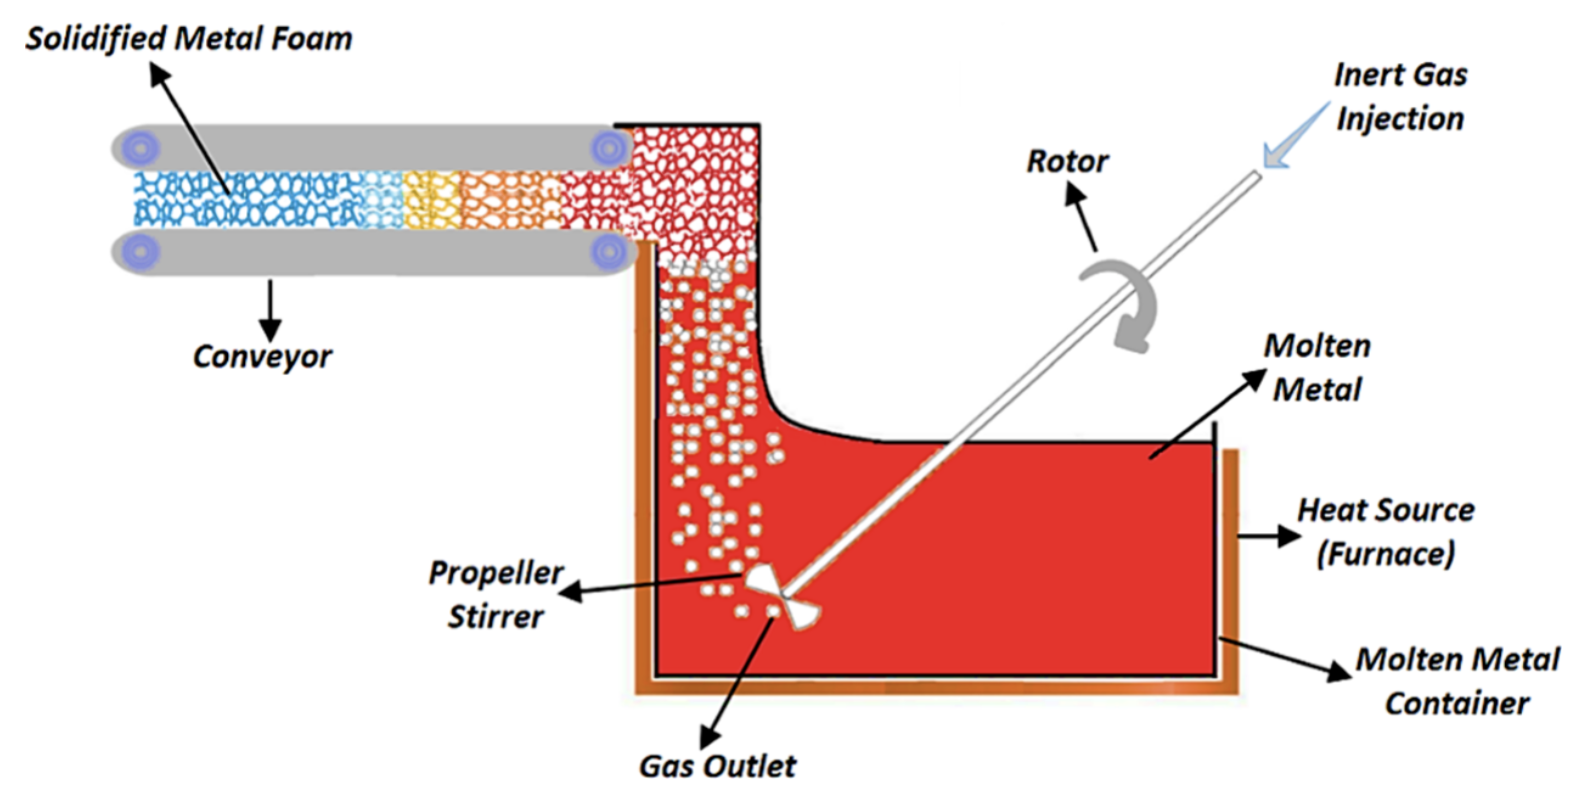
\includegraphics[width=12cm]{vyroba_1.png}
  \centering
  \caption{Diagram of metal gas injection techniques \cite{Hassan2024}.}
  \label{fig:vyroba_1}
\end{figure}


\noindent An alternative method for producing metallic foam involves directly foaming metal melts using a blowing agent, rather than introducing gas into the melts as traditionally practiced. 
This technique relies on the controlled decomposition of a blowing agent upon heating, which releases gas to initiate foaming of the molten metal. 
The process is conducted in two stages: first, heating the metal to its melting point, and then adding and mixing the blowing agent with the molten metal using a propeller stirrer to achieve uniform foam. 
The effectiveness of this method hinges on selecting an appropriate blowing agent capable of generating sufficient gas bubbles. This approach typically results in a closed-cell structure and is influenced by factors such as particle surface contacts, matrix alloy composition, and thermal processing conditions. 
Since the 1950s, hydrides like TiH2 have been the most effective blowing agents, though their high cost has prompted exploration of cheaper alternatives like carbonates. 
The general decomposition reactions for hydrides and carbonates release hydrogen and CO2 gas, respectively. The ALPORAS aluminum foam, produced using this technique by Shinko Wire, Japan, since 1986, exemplifies this method, with the quality of the foam depending on factors such as the distribution of the blowing agent, thickening agent effects, melting temperature, stirring speed, and cooling rate.
Figure \ref{fig:vyroba_2} illustrates the schematic of the manufacturing process of ALPORAS.

\begin{figure}[h]
  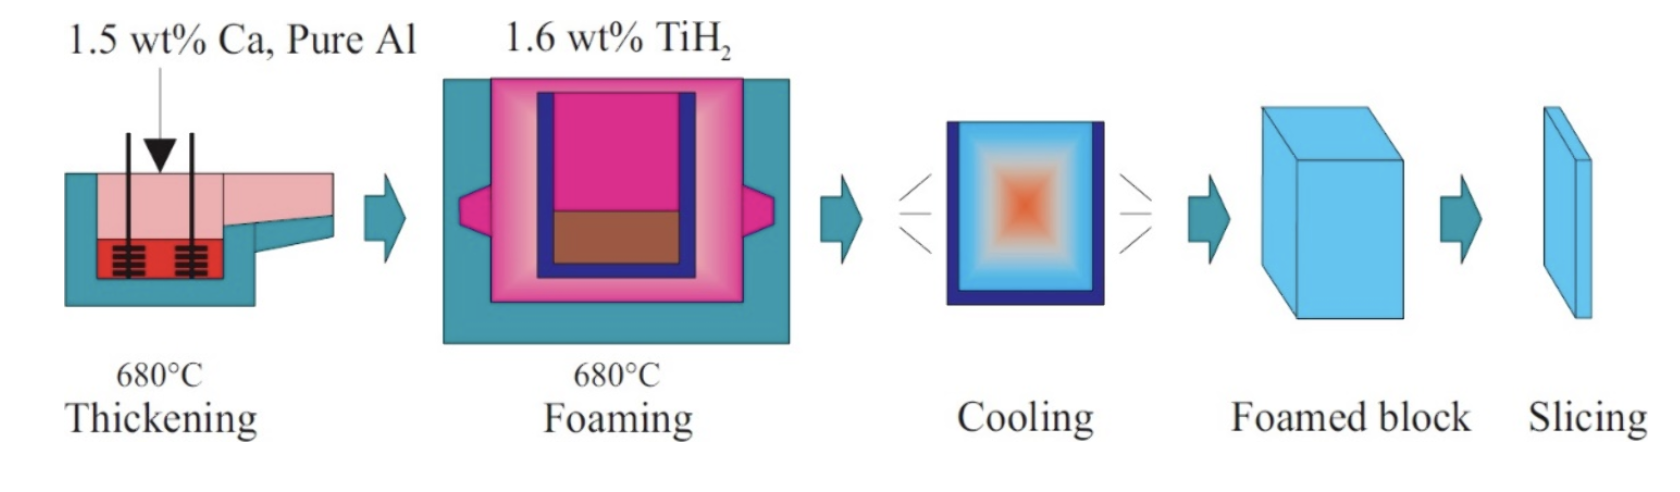
\includegraphics[width=12cm]{vyroba_2.png}
  \centering
  \caption{Diagram of the Manufacturing Process of ALPORAS \cite{Miyoshi}.}
  \label{fig:vyroba_2}
\end{figure}
\pagebreak
\noindent Figure \ref{fig:vyroba_3} shows the titanium wire space holder method for the fabrication of metallic foam.
The space holder or infiltration method for creating metallic foam involves introducing temporary space holders into a metal matrix, which are subsequently removed through leaching or thermal treatment, resulting in lightweight, porous metals with structural gaps, often referred to as "syntactic foam." This technique is employed to manufacture homogeneous, interconnected porous structures, utilizing materials like woven wire mesh, salt beads, hollow spheres, ceramics, and polymers as space holders. The process begins with molding and sintering the space holder particles, followed by melting the metal and infusing it into the space holder structure. After solidification, the space holders are removed to leave behind a porous metallic foam. The infiltration method is particularly favored when a liquid metallurgical approach is used. In cases involving woven wire, pre-molding and sintering steps are often omitted; instead, a 3D-mesh structure is directly filled with molten metal. This method, though challenging, is notably used in orthopedic applications due to its ability to produce structurally complex foams with significant mechanical, thermal, acoustic, electrical, and chemical properties.

\begin{figure}[h]
  \centering
  \begin{minipage}{0.5\textwidth}
      \centering
      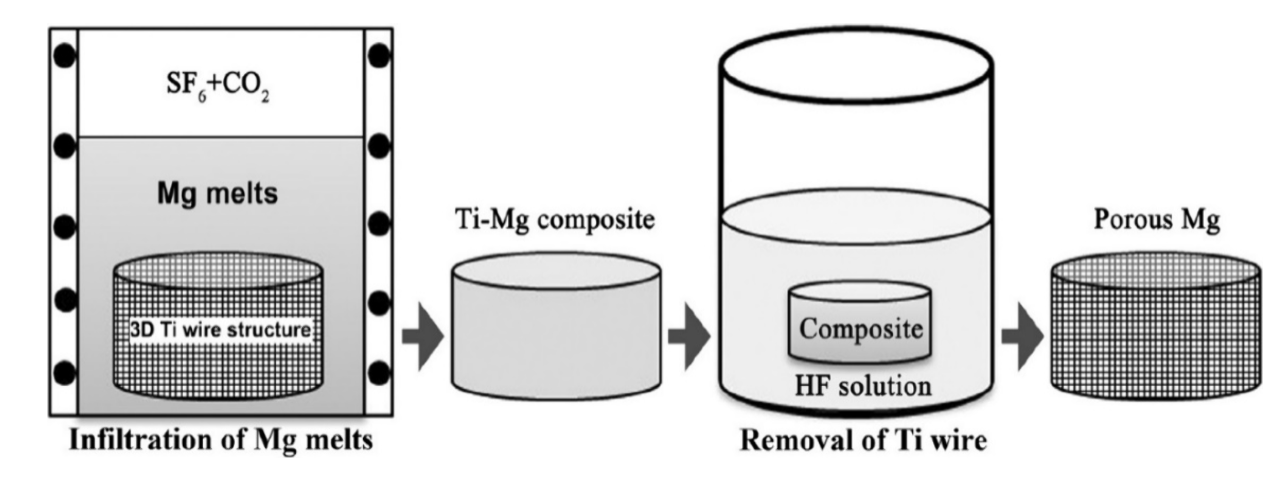
\includegraphics[height=3cm]{vyroba_3.png}
      \caption{The wire space holder \cite{Jiang2014}.}
      \label{fig:vyroba_3}
  \end{minipage}\hfill
  \begin{minipage}{0.5\textwidth}
      \centering
      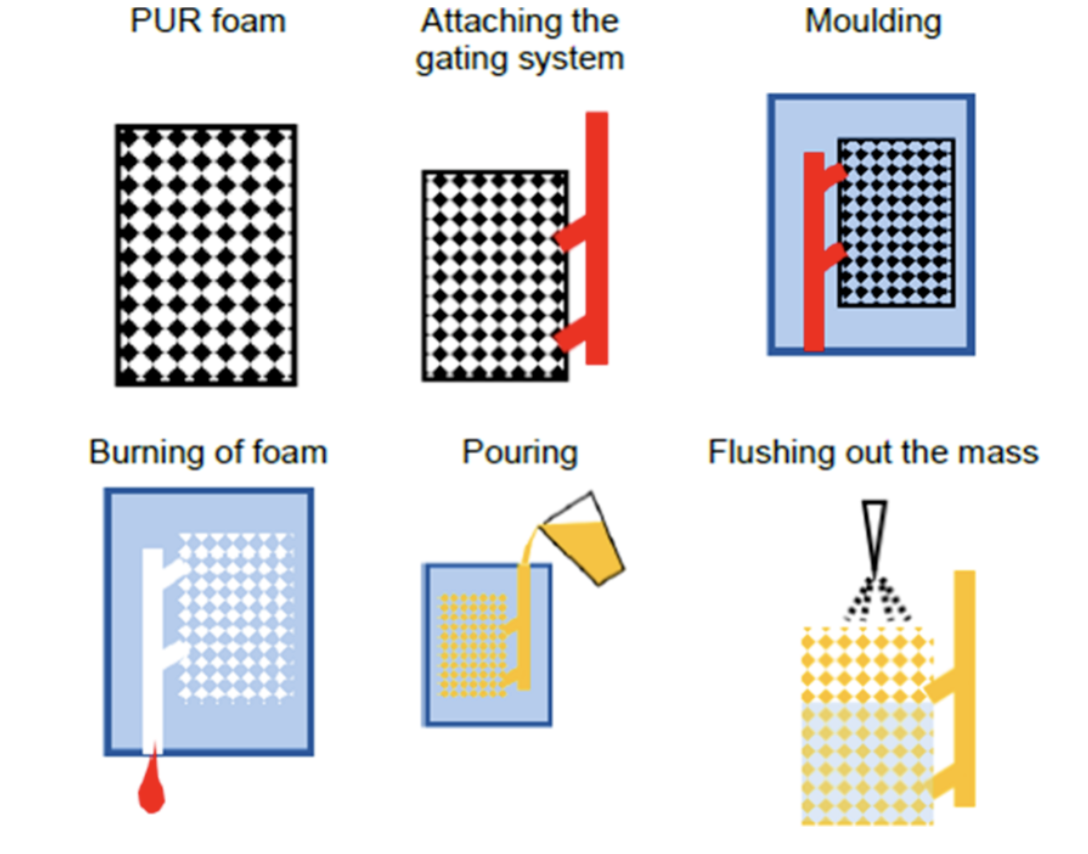
\includegraphics[height=4cm]{vyroba_4.png}
      \caption{The investment casting process \cite{Cooper2014}.}
      \label{fig:vyroba_4}
  \end{minipage}
\end{figure}

\noindent The investment casting method for producing open-cell metallic foam involves using foams as templates to achieve precise and detailed structures. This technique begins with creating a polymeric sponge or foam, typically polyurethane, which serves as a negative mold for the final metallic foam. 
The polymeric foam is then coated with a slurry made from heat-resistant materials like mullite, phenolic resin, and calcium carbonate or a gypsum-based mixture. After the slurry dries and cures, the polymeric foam is removed through heat treatment, leaving behind a mold for the metallic foam. Molten metal is cast into this mold, replicating the original foam structure, and solidifies to form the final metallic foam. 
The mold is subsequently removed using solvents, heat, pressurized water, or other methods, revealing the desired foam. Despite its effectiveness, this method faces challenges in ensuring complete mold filling and removal without damaging the intricate structure due to high porosity. 
Companies such as ERG Aerospace Corporation produce various metallic foams under the trade name “Duocel,” including copper, aluminum, brass, and more, with densities ranging from 3 to 12~\% and porosities from 80~\% to 97~\%. 
The investment casting method is shown in Figure \ref{fig:vyroba_4}.

\subsubsection{Powder (solid) metallurgy}
Unlike the liquid melt route, an alternative method for fabricating metallic foam, patented in the late 1950s, involves processing metal in its solid form. This technique utilizes metallic powder, which remains solid throughout the process, to produce the foam. By employing sintering and solid-state operations, an open-cell structure is achieved. The initial size and shape of the powder are critical to the final foam structure, as they influence the resulting morphology. In contrast to liquid-state processes, which often produce closed pores due to surface tension, the sintering method yields an open structure with isolated spherical particles linked by sintered necks. This method is particularly effective for metals with high melting points and is well-suited for reactive metals.
\\
\\
\noindent In the 1990s, German scientists developed a solid-state route, known as the Fraunhofer process, for fabricating metallic foam. This method starts with blending metal powders and blowing agents to form a dense precursor. The precursor is then heated, causing the blowing agent to decompose and release gas, which creates foam with an open-cell structure. Key challenges include ensuring even distribution of the blowing agent and avoiding premature decomposition. Common blowing agents include hydrides like TiH2, although carbonates are being explored as cost-effective alternatives. This process results in foams with cell diameters ranging from 1 mm to 5 mm, with expansion times varying based on precursor size and furnace temperature.
An example of this method applied to copper foam manufacturing is shown in Figure \ref{fig:vyroba_5}.

\begin{figure}[h]
  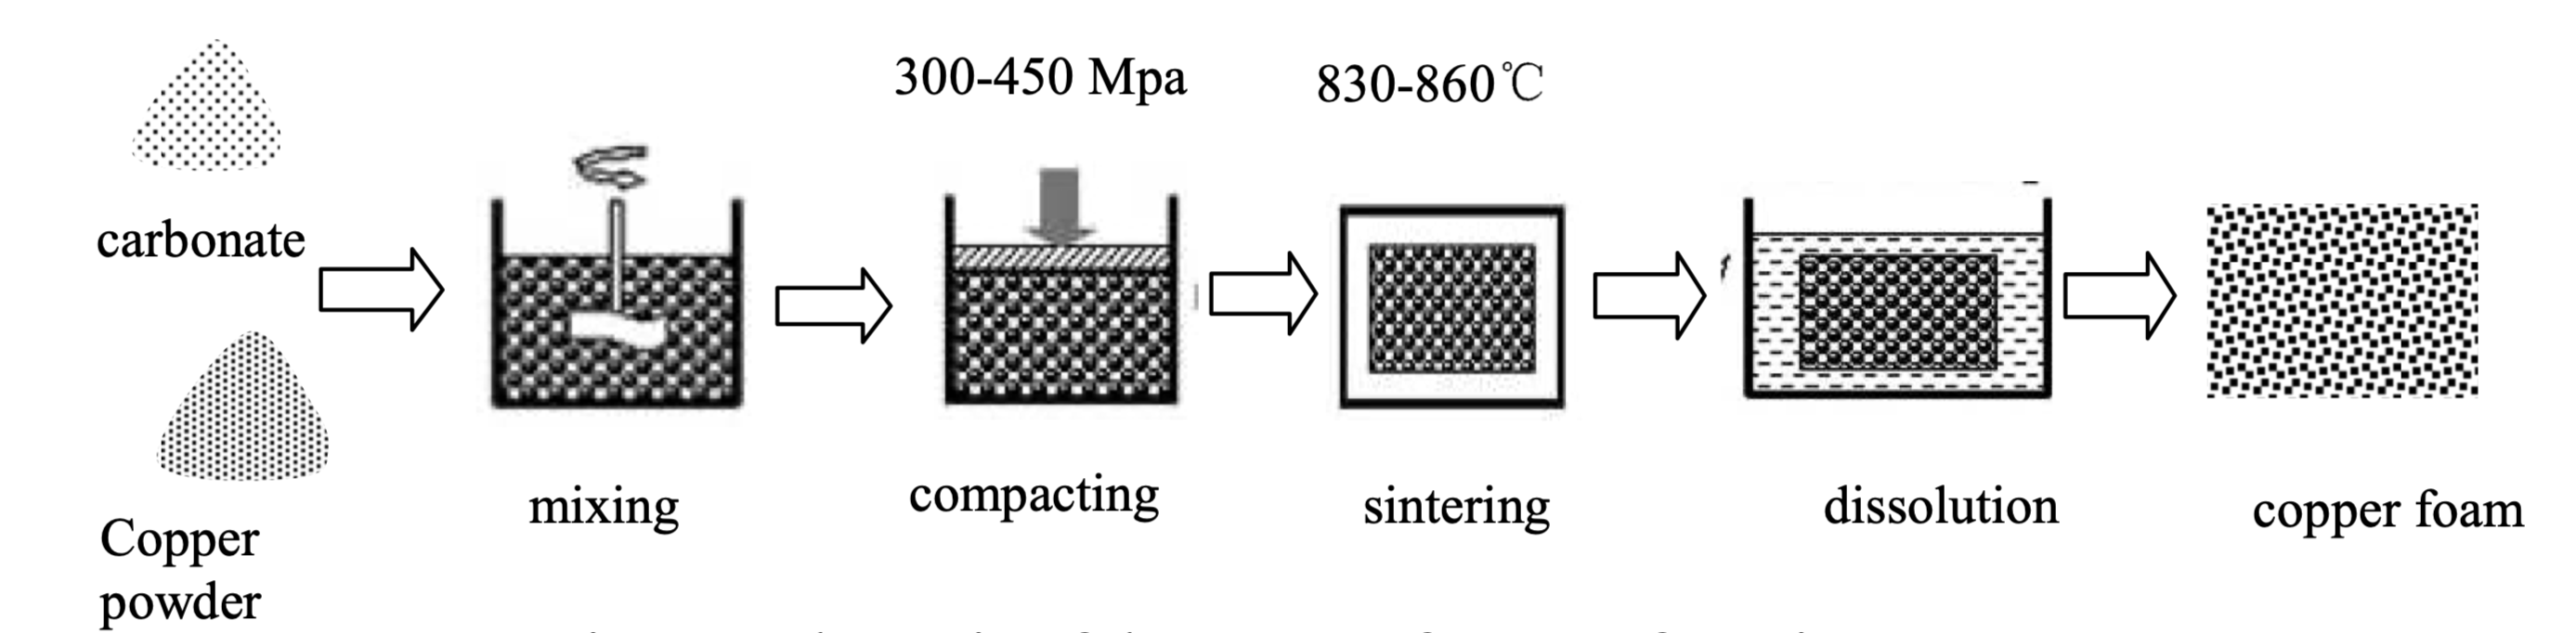
\includegraphics[width=12cm]{manufacturing_1.png}
  \centering
  \caption{Schematic of the process for manufacturing porous copper \cite{Zhou2013}.
  }
  \label{fig:vyroba_5}
\end{figure}

\noindent The space holder method, shown in Figure \ref{fig:vyroba_6} involves infusing liquid metal into molds containing space-holding materials such as wire mesh, salt beads, hollow spheres, ceramics, and polymers. A notable patented method from 1962 uses metal powder combined with space holders to produce metallic foam. The process begins by mixing metal powder, space holders, and binders, followed by compaction to form a dense precursor. Space holders are then removed either through thermal degradation or dissolution, depending on their melting points. Thermal degradation uses space holders like PMMA or carbamide, which degrade below the metal's sintering temperature, while dissolution involves space holders with higher melting points like NaCl, which are removed after sintering. The resulting foam's structure is influenced by space holder size, shape, volume fraction, and process parameters.
\\
\\
\noindent The Gas Entrapment Technique for producing metallic foam, patented by Kearns in the late 1980s, offers an alternative to traditional methods involving melting or blowing agents. This method is especially suitable for highly reactive metals with high melting points. The process starts with filling a shell with metal powder, followed by removing air and backfilling with inert gas, typically argon, at high pressure. The shell is then sealed and subjected to hot isostatic pressing, which ensures uniformity and creates high internal pressure due to gas entrapment. Finally, the shell undergoes heat treatment at temperatures above 60~\% of the metal's melting point. This sophisticated technique, also adopted by Boeing for titanium foam in aircraft panels, highlights its potential for diverse applications in both research and industry.
The technique diagram is shown in Figure \ref{fig:vyroba_7}

\begin{figure}[h]
  \centering
  \begin{minipage}{0.6\textwidth}
      \centering
      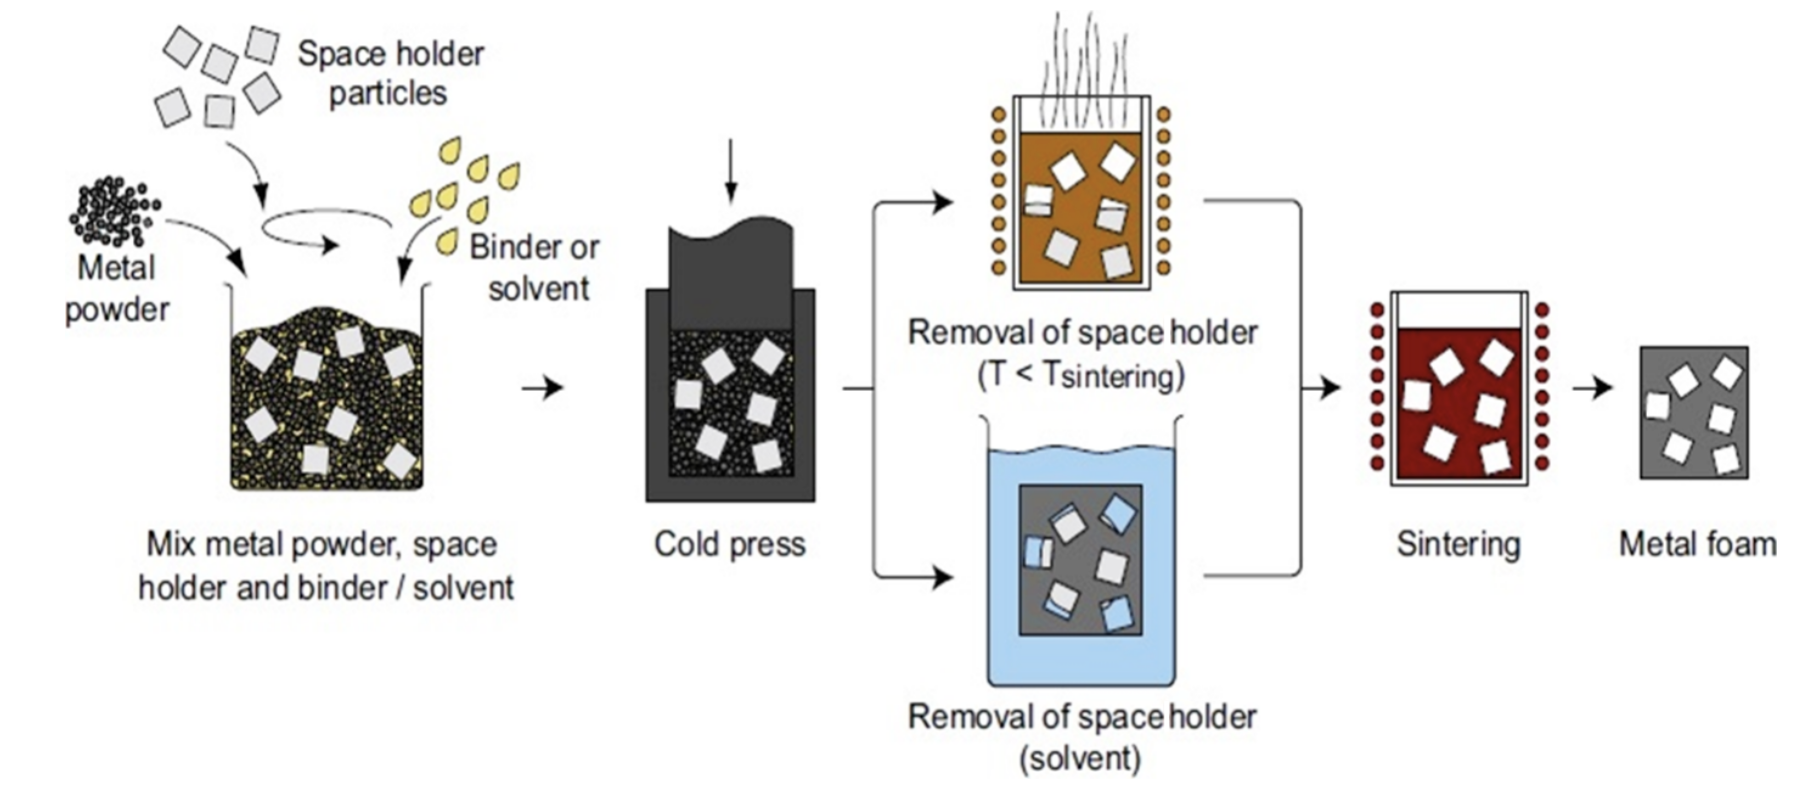
\includegraphics[height=4cm]{vyroba_6.png}
      \caption{The space holder method \cite{Goodall2014}.}
      \label{fig:vyroba_6}
  \end{minipage}\hfill
  \begin{minipage}{0.4\textwidth}
      \centering
      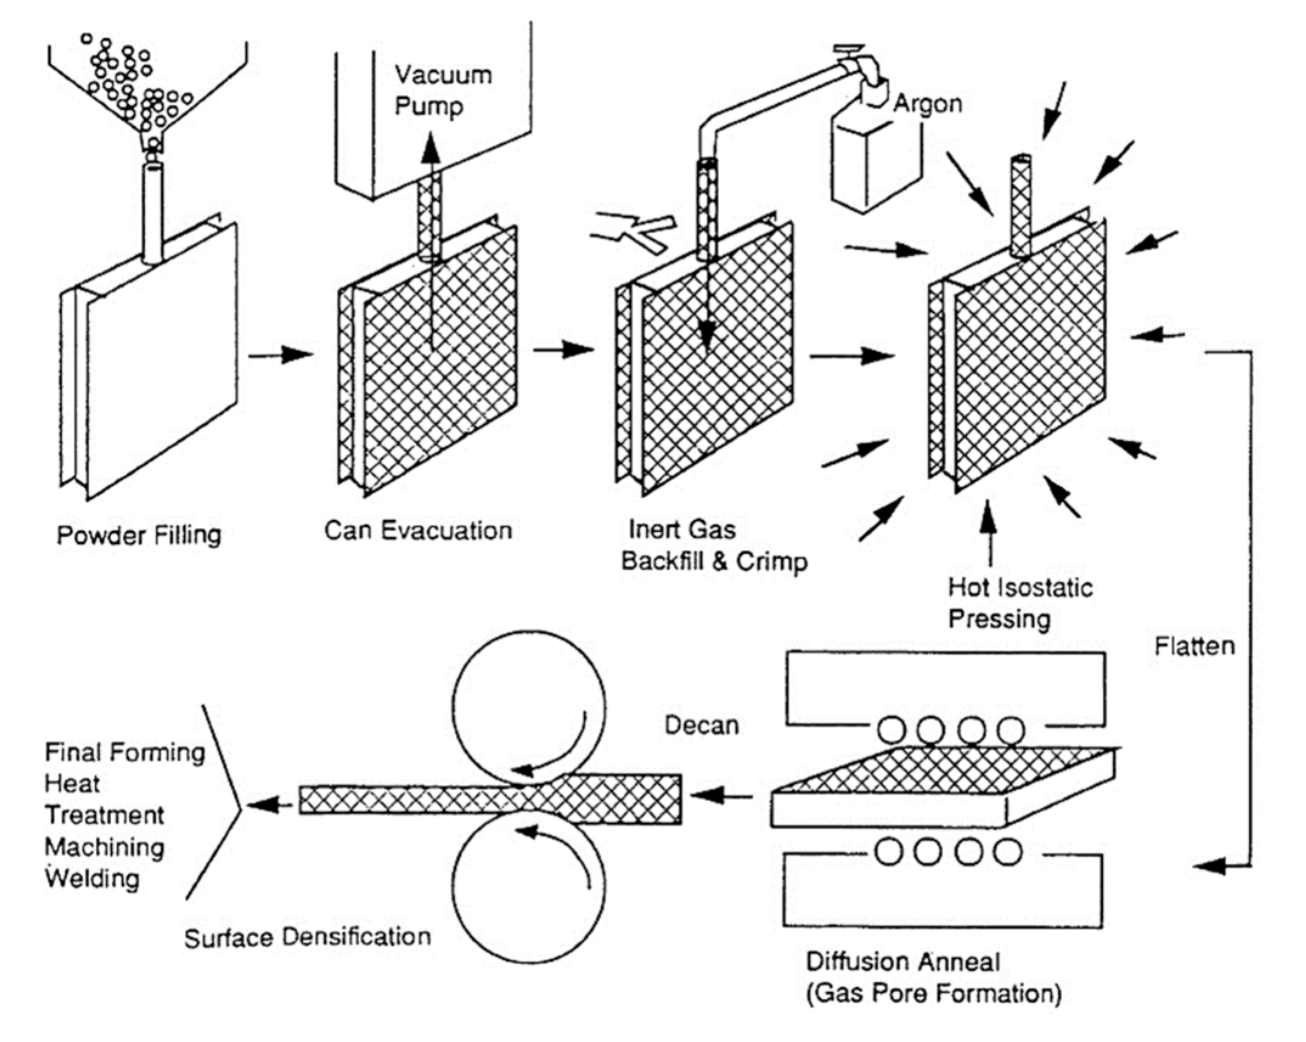
\includegraphics[height=5cm]{vyroba_7.png}
      \caption{The gas entrapment technique \cite{Banhart2001}.}
      \label{fig:vyroba_7}
  \end{minipage}
\end{figure}
\subsubsection{Metal vapor deposition}
\noindent Metal vapor deposition is a notable technique for producing metallic foam, starting with a robust precursor, usually polyurethane (PU), that defines the foam's shape. The process involves generating metal vapor by heating metal in a vacuum chamber, then condensing this vapor onto the polymeric substrate. The polymer is subsequently removed through heat treatment, followed by sintering in a furnace to achieve the metallic foam structure. This technique can be executed using Chemical Vapor Deposition (CVD) or Physical Vapor Deposition (PVD). CVD involves the thermal decomposition of metal carbonyl gases which condense on the substrate, as used by Inco Limited to produce nickel foam branded as "Inco foam." PVD methods, such as metal spray deposition or arc-vapor deposition, involve depositing solid metal forms onto the substrate. The final foam's characteristics depend on vapor density and exposure time \cite{Queheillalt2001}.
\subsubsection{Metal ion solution}
\noindent Electrochemical Deposition (Metal Ion Solution) is a technique used to produce metallic foam, leveraging principles similar to vapor deposition and investment casting. This method begins with a polymeric foam, which serves as the cathode electrode in an electrochemical cell, while a metal anode electrode dissolves and deposits metal onto the foam. The polymeric foam, which must be made conductive through electroless plating or a thin conductive layer, then undergoes electroplating to form a metallic layer. After the polymer is removed through heat treatment, the metal foam is sintered to achieve the final porous structure. Unlike solid frameworks from investment casting, this process creates a hollow framework. Figure \ref{fig:vyroba_8} shows the diagram of metal ion solution manufacturing method \cite{Banhart2001}.

\begin{figure}[h]
  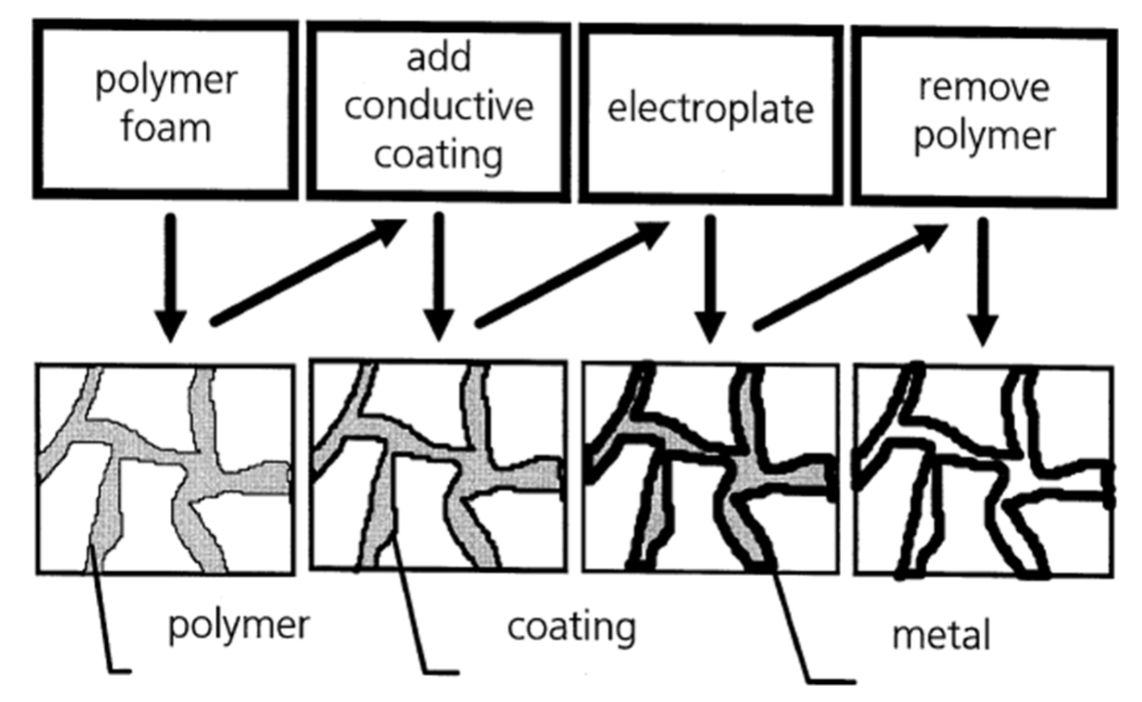
\includegraphics[width=7cm]{vyroba_8.png}
  \centering
  \caption{Schematic of electrochemical technique for production of metallic foam \cite{Hassan2024}.
  }
  \label{fig:vyroba_8}
\end{figure}

\pagebreak
\section{Numerical simulation of flow through porous materials}
For the viscous behavior, there are several different approaches to numerically solve the porous medium domain.
Three main ways are introduced: simulating the porous zone as a region with additional terms in the momentum equation, modelling a substitute geometry to recreate the viscous and thermal behavior of porous material and the most challenging way - scanning the porous material structure to get a precise digital geometry copy for FEA analysis.
\\
\\
\noindent In the case of heat transfer and two phase flow with boiling regimes simulation, porous materials represent a very challenging task.
An overview of previous research shown in Table \ref{table:prehled_pen} shows there no publication in both "2-phase" and "Numerical" category.
Complex fluid behavior such as the capillary effect of boiling in porous structure are on the edge of the present CFD software abilities.
A study by K.S. Bibin was published in 2022 on the topic of boiling in porous structure, simulated in OPENFoam on a simplified geometry case \cite{Bibin2022}. 
A more recent article published in 2024 by Y. Kang describes the pool boiling in porous copper structure, a simplified structure of the porous microchannels was modelled in ANSYS Fluent, representing one of the few numerical two phase studies \cite{Kang2024}.

\subsection{Darcy–Forchheimer equation}
Darcy-Forchheimer equation (Eq. \ref{eq:DF}) describes the pressure drop of porous media as a term in the momentum equation.
Empirical equations are needed to describe the Darcy-Forchheimer coefficients, they are strictly dependent on the microstructure and geometrical measures of the porous material.
Equations \ref{eq:DF2} and \ref{eq:DF3} by Calmidi \cite{Calmidi} and Yang \cite{Yang2021} evaluate the permeability \textit{K} and Forchheimer coefficient \textit{c} of porous metal material in relation to the diameter of the pores, the diameter of the struts, and the porosity of the material.
The previous research focused on CFD simulation of porous copper material by using the empirical correlations by Yang\cite{Yang2021} applied to the ANSYS Fluent 2023.1 numerical simulation.
Many of the empirical equations described by Yang were considered and the results of the numerical analysis are compared with the experimental data, but only the mentioned equations provided feasible results for the porous structure used.
Given the variability in pressure drop results across different correlations, it can be concluded that porosity or PPI (pores per inch) alone are insufficient to fully characterize the viscous behavior of porous materials. A precise match in the microstructure of the porous zone is essential for a more accurate specification.\\
\\

Momentum equation:
\begin{equation}
  \rho \frac{Du}{Dt} = -\nabla p + \nabla \cdot \tau + \rho f
\end{equation}
where $\rho$ is the fluid density, $u$ is the velocity vector, $p$ is the static pressure, $\tau$ is the viscous stress tensor and $f$ represents body forces per unit mass.


Darcy-Forchheimer equation:

\begin{equation}
    \nabla p = \left( \dfrac{\mu}{K}  + \rho \dfrac{c}{\sqrt{K}} U   \right)U
\label{eq:DF}
\end{equation}
Here, $\mu$ is the dynamic viscosity, $K$ is the intrinsic permeability, $c$ is the Forchheimer coefficient and $U$ is the superficial velocity. The first term represents viscous Darcy resistance and the second term accounts for inertial losses.

Permeability \cite{Yang2021}\cite{Calmidi}:

\begin{equation}
    K = d_p^2 \cdot 0.00747(1-\epsilon)^{-0.2329} \left(\dfrac{d_f}{d_p}\right)^{-0.00249}
    \label{eq:DF2}
\end{equation}

Forchheimer coefficient \cite{Yang2021}\cite{Calmidi}:
\begin{equation}
    c = 0.00212(1-\epsilon)^{-0.132} \left(\dfrac{d_f}{d_p}\right)^{-1.63}
    \label{eq:DF3}
\end{equation}

\pagebreak
\subsection{Substitute geometry}

The simplification of porous structures into substitute geometries is a modeling approach that helps to predict fluid dynamics and pressure drops in complex porous media. The model translates intricate real-world porous structures, like the metallic foams, into a simplified geometric framework. 
This method is beneficial for studying fluid flow in media with high porosity, such as metal foams used in applications like heat exchangers or flow control devices. 
The goal of simplification is to facilitate mathematical modeling, providing more accurate predictions of fluid behavior, such as the pressure gradients during flow through porous media \cite{DuPlessis1988}\cite{DuPlessis1994}.
\\
\\
\noindent The method relies on the concept of a representative unit cell (RUC), which serves as a simplified geometric representation of the complex porous structure. The RUC is designed to replicate the main flow characteristics and geometric traits of the porous medium. 
In this particular case, the simplified geometry is often modeled using a rectangular or square arrangement, mimicking the strands and pores of metallic foams. The RUC incorporates critical parameters such as pore size, porosity, and the cross-sectional shape of the foam's internal structure. 
An example of three different RUC geometries is shown in Figure \ref{fig:RUC}.
By employing this geometry, the behavior of fluid flow under different regimes, including low-velocity Darcy flow and high-velocity Forchheimer flow, can be analytically or numerically explored.
\begin{figure}[h]
  \centering
  \begin{minipage}[b]{0.3\textwidth}
      \centering
      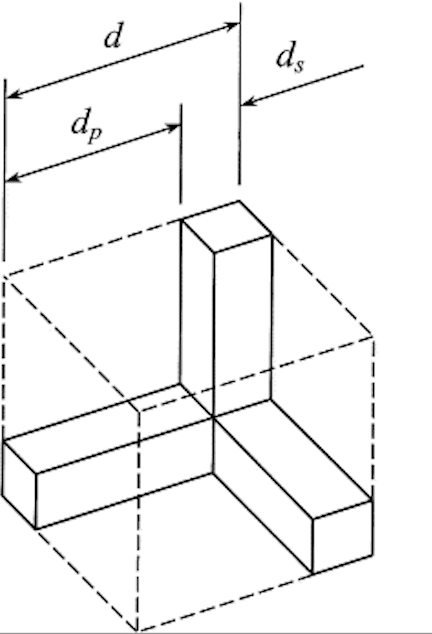
\includegraphics[height=4cm, trim= 0 2 0 0, clip]{struktura_peny3.png}
      \caption*{RUC for foam structure \cite{GFourie2002}.}
  \end{minipage}
  \hfill
  \begin{minipage}[b]{0.3\textwidth}
      \centering
      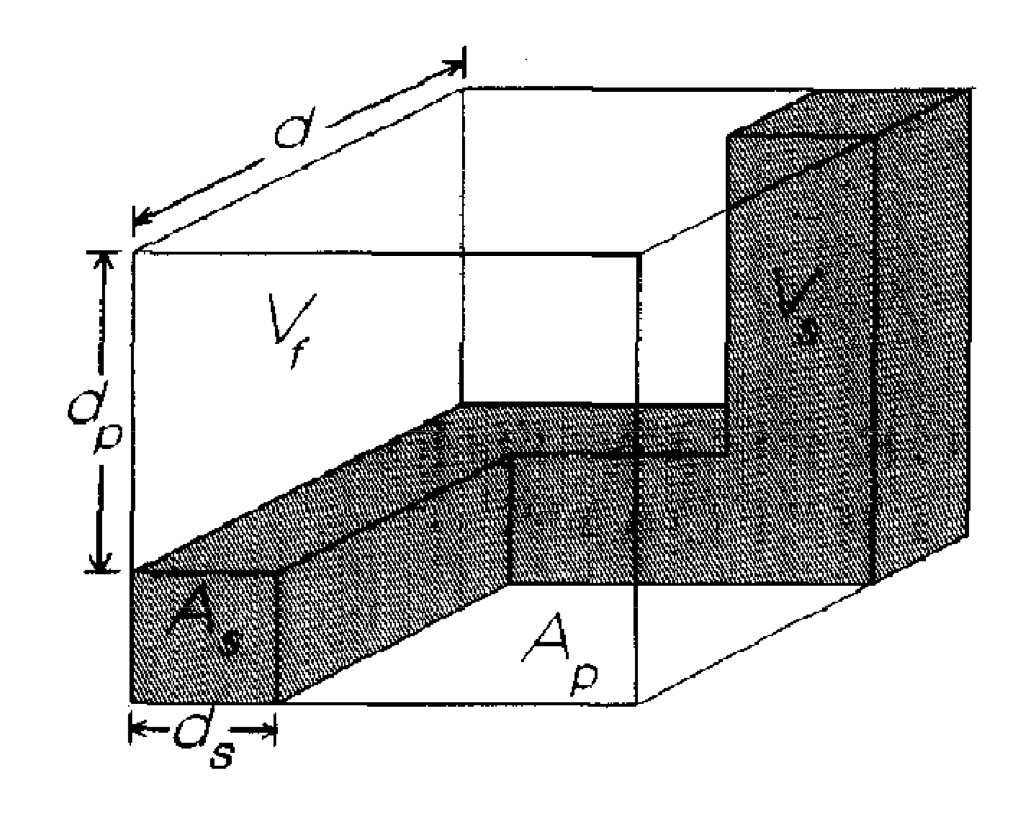
\includegraphics[width=\textwidth]{struktura_peny1.png}
      \caption*{RUC for foam structure \cite{DuPlessis1994}.}
  \end{minipage}
  \hfill
  \begin{minipage}[b]{0.35\textwidth}
      \centering
      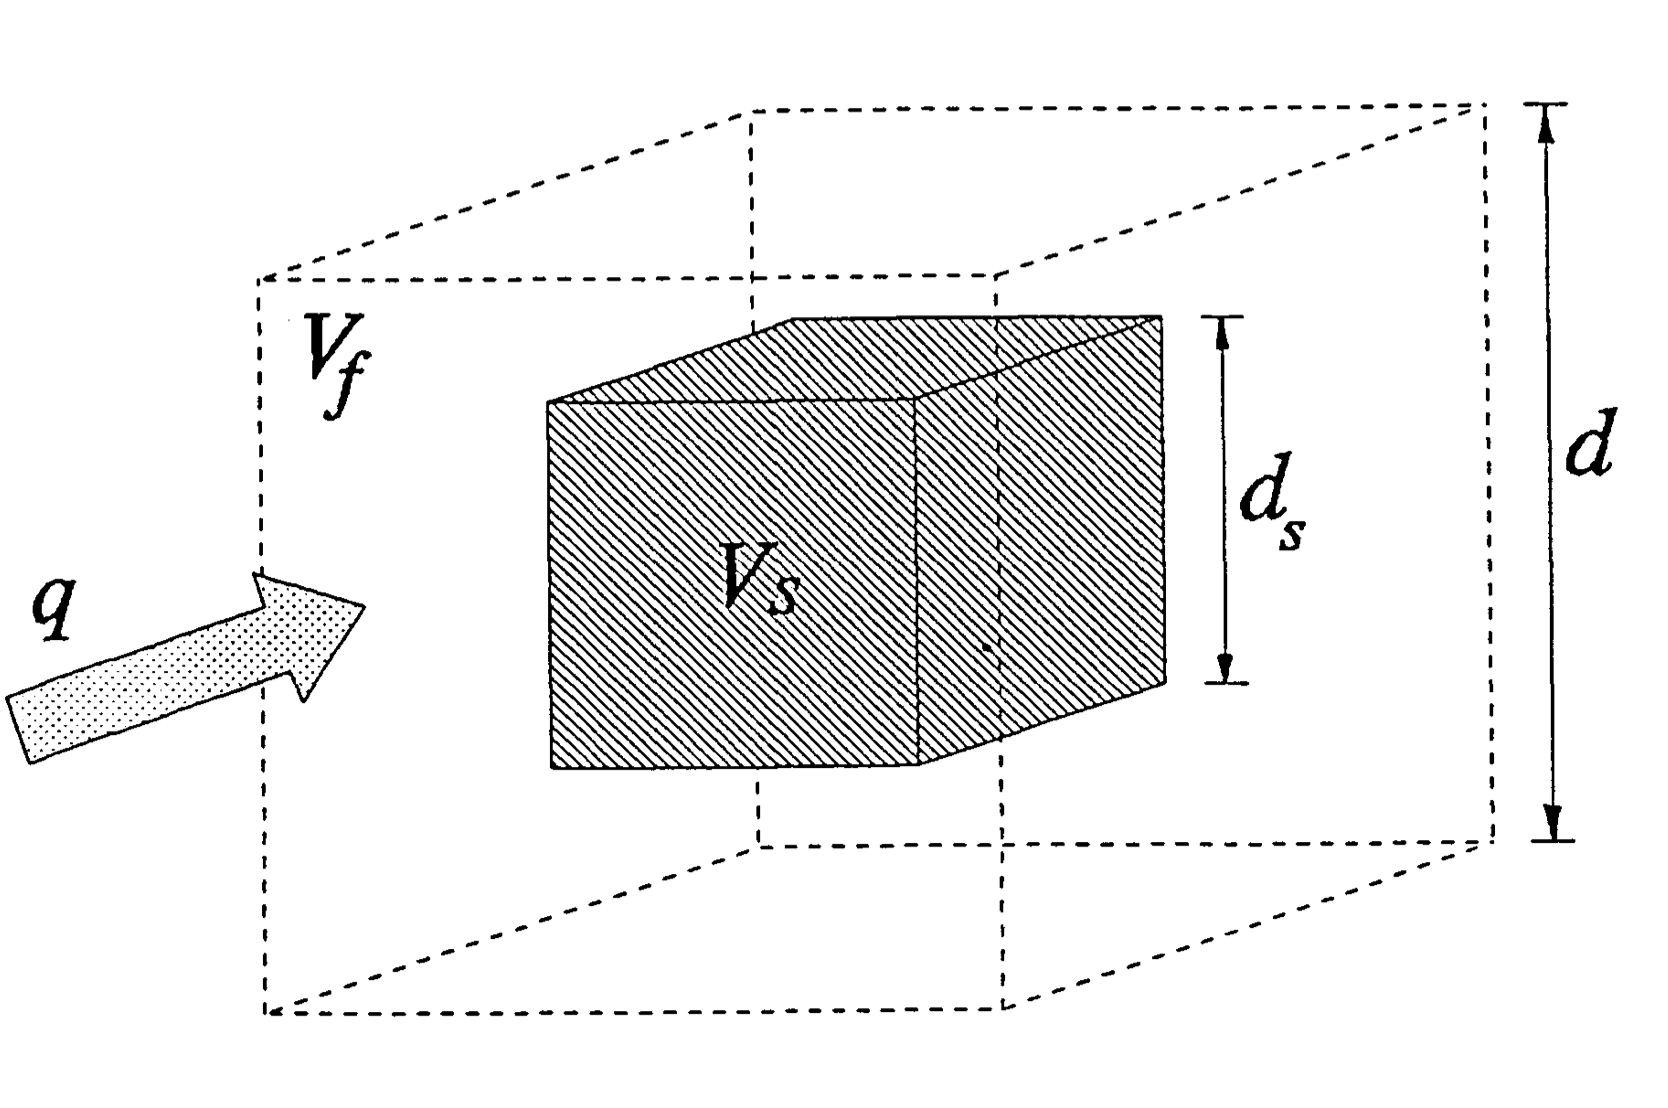
\includegraphics[width=\textwidth]{struktura_peny2.png}
      \caption*{RUC for granular structure \cite{DuPlessis1988}.}
  \end{minipage}
  \caption{Cubic representative unit cells [RUC].}
  \label{fig:RUC}
\end{figure}

\noindent An article by J.G. Fourie gives a detailed theoretical analysis and experimental validation of the substitute geometry method.
The simplified RUC model successfully predicts pressure drops across metallic foams under various flow conditions. It translates the complex interfacial geometry into a manageable framework while capturing the correct hydrodynamic conditions. The pressure gradient predictions show good alignment with experimental data for both Darcy and Forchheimer flow regimes, as demonstrated by comparison with empirical studies \cite{GFourie2002}.
\\
\\
\noindent The approach enhances the modeling process by introducing characteristic dimensions such as the representative hydraulic diameter (RHD), which accounts for the hydrodynamic effects of the triangular cross-sectional shape of the foam strands and material clustering at strand vertices. This method improves upon earlier models by eliminating the need for prior experimental calibration of foam-specific flow behaviors.
The results of the model were validated against experimental data from metallic foam samples of various porosities and cell sizes. The method shows that it can accurately predict pressure gradients without the necessity for prior knowledge of the specific flow behavior of the porous medium, making it highly adaptable and reliable for real-world applications.
In conclusion, the method of simplifying porous structures into substitute geometries offers a robust and efficient way to predict fluid behavior in highly porous materials. It simplifies the complexity of real-world structures while maintaining a high level of accuracy.

\pagebreak
\subsection{Microstructure scanned by microtomography}
The complex method of CFD modeling in 3D-scanned porous materials is described on the example of microtomography ($\mu T$).
The study "Microtomography-based CFD Analysis of Transport in Open-Cell Aluminum Metal Foams" by Paola Ranut et al. (2014) focuses on the CFD analysis of transport properties in open-cell aluminum foams \cite{Ranut2014}.
Figure \ref{fig:mikrotomo} shows the used aluminum porous foam and the numerical mesh generated by ANSYS ICEM CFD.
For the CFD simulations the commercial software ANSYS CFX 13.0 was used.
\begin{figure}[h]
  \centering
  \begin{minipage}[b]{0.2\textwidth}
      \centering
      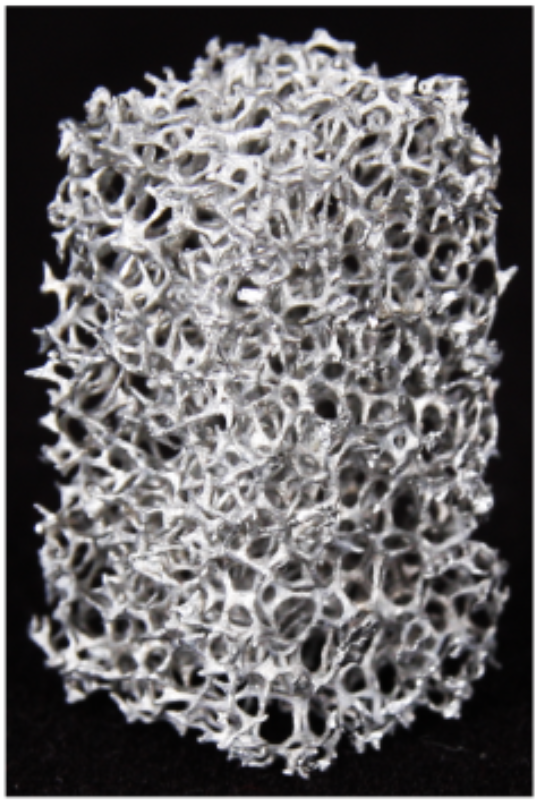
\includegraphics[height=5cm, trim= 0 2 0 0, clip]{fotka_vzorku.png}
      \caption*{Al foam}
  \end{minipage}
  \hfill
  \begin{minipage}[b]{0.3\textwidth}
      \centering
      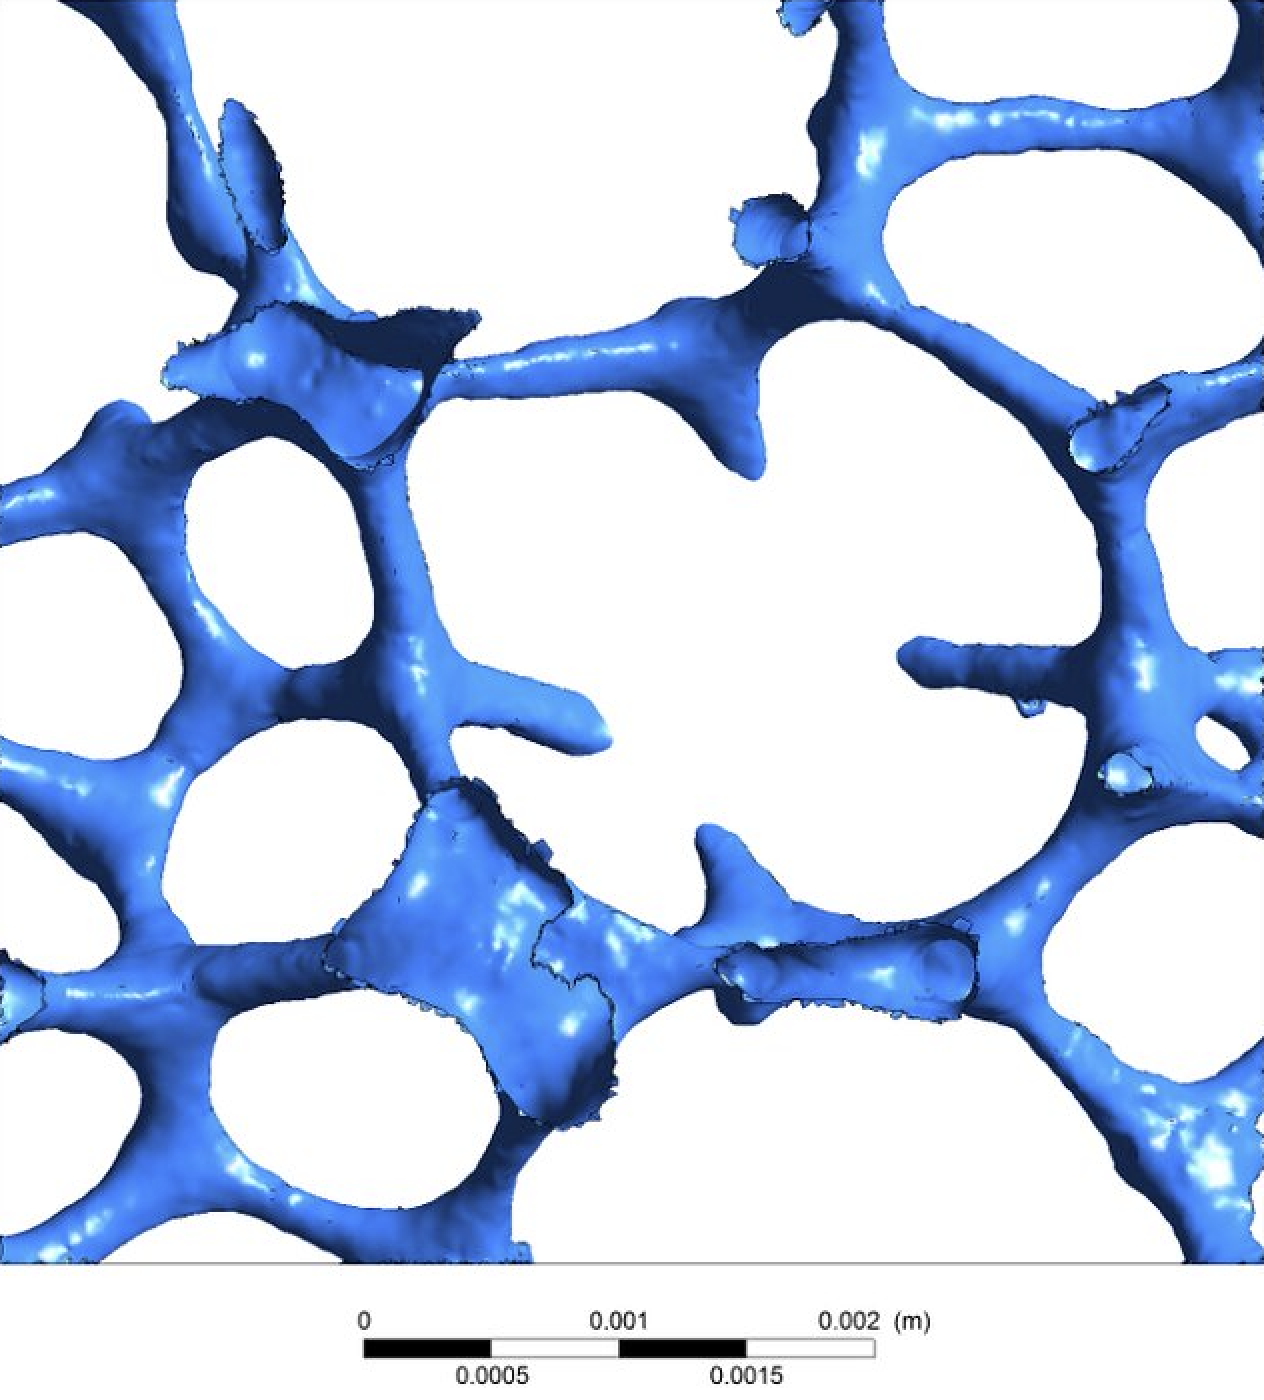
\includegraphics[width=\textwidth]{detail_skenu.png}
      \caption*{scanned structure}
  \end{minipage}
  \hfill
  \begin{minipage}[b]{0.45\textwidth}
      \centering
      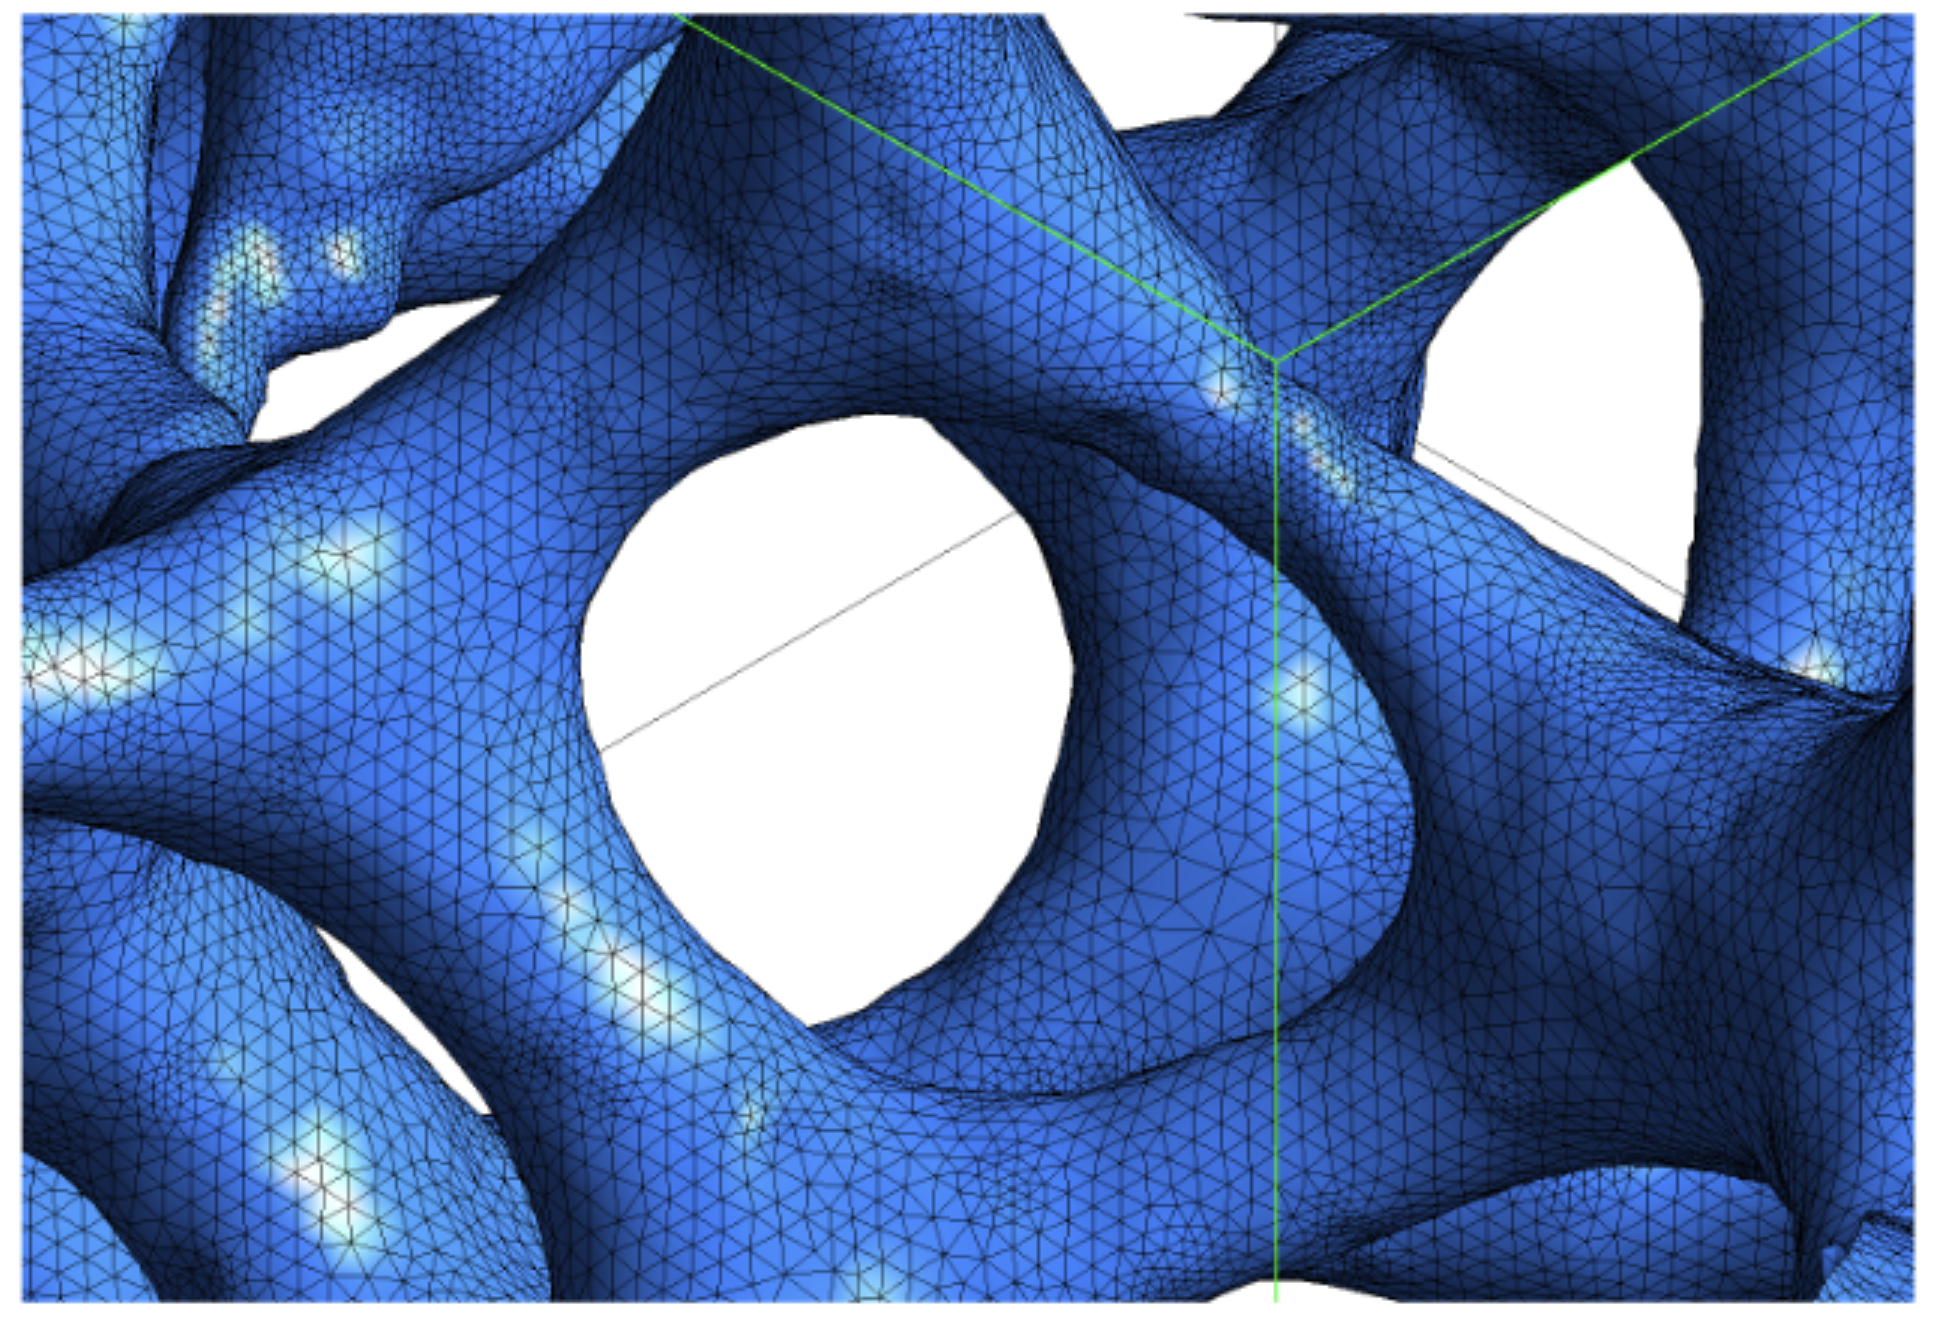
\includegraphics[width=\textwidth]{sit.png}
      \caption*{mesh detail}
  \end{minipage}
  \caption{Porous structure (30 PPI) scanned by $\mu$CT and meshed for the CFD analysis \cite{Ranut2014}.}
  \label{fig:mikrotomo}
\end{figure}

\noindent The study calculates the permeability and form drag coefficient for each foam. At low Reynolds numbers, pressure drop varies linearly with velocity, while at higher velocities, inertial effects dominate. The Darcy-Forchheimer law accurately describes these effects.
Heat transfer coefficients increase with pore density. The study demonstrates that the thermal conductivity of the foam is mainly influenced by the solid ligaments, with the fluid phase contributing only marginally.
The results validate the use of µ-CT coupled with CFD for accurately simulating and characterizing open-cell metal foams. These findings contribute to better design strategies for heat transfer devices, offering a balance between enhanced performance and pressure loss. The method can be applied to other porous materials for broader engineering applications​
\begin{figure}[h]
  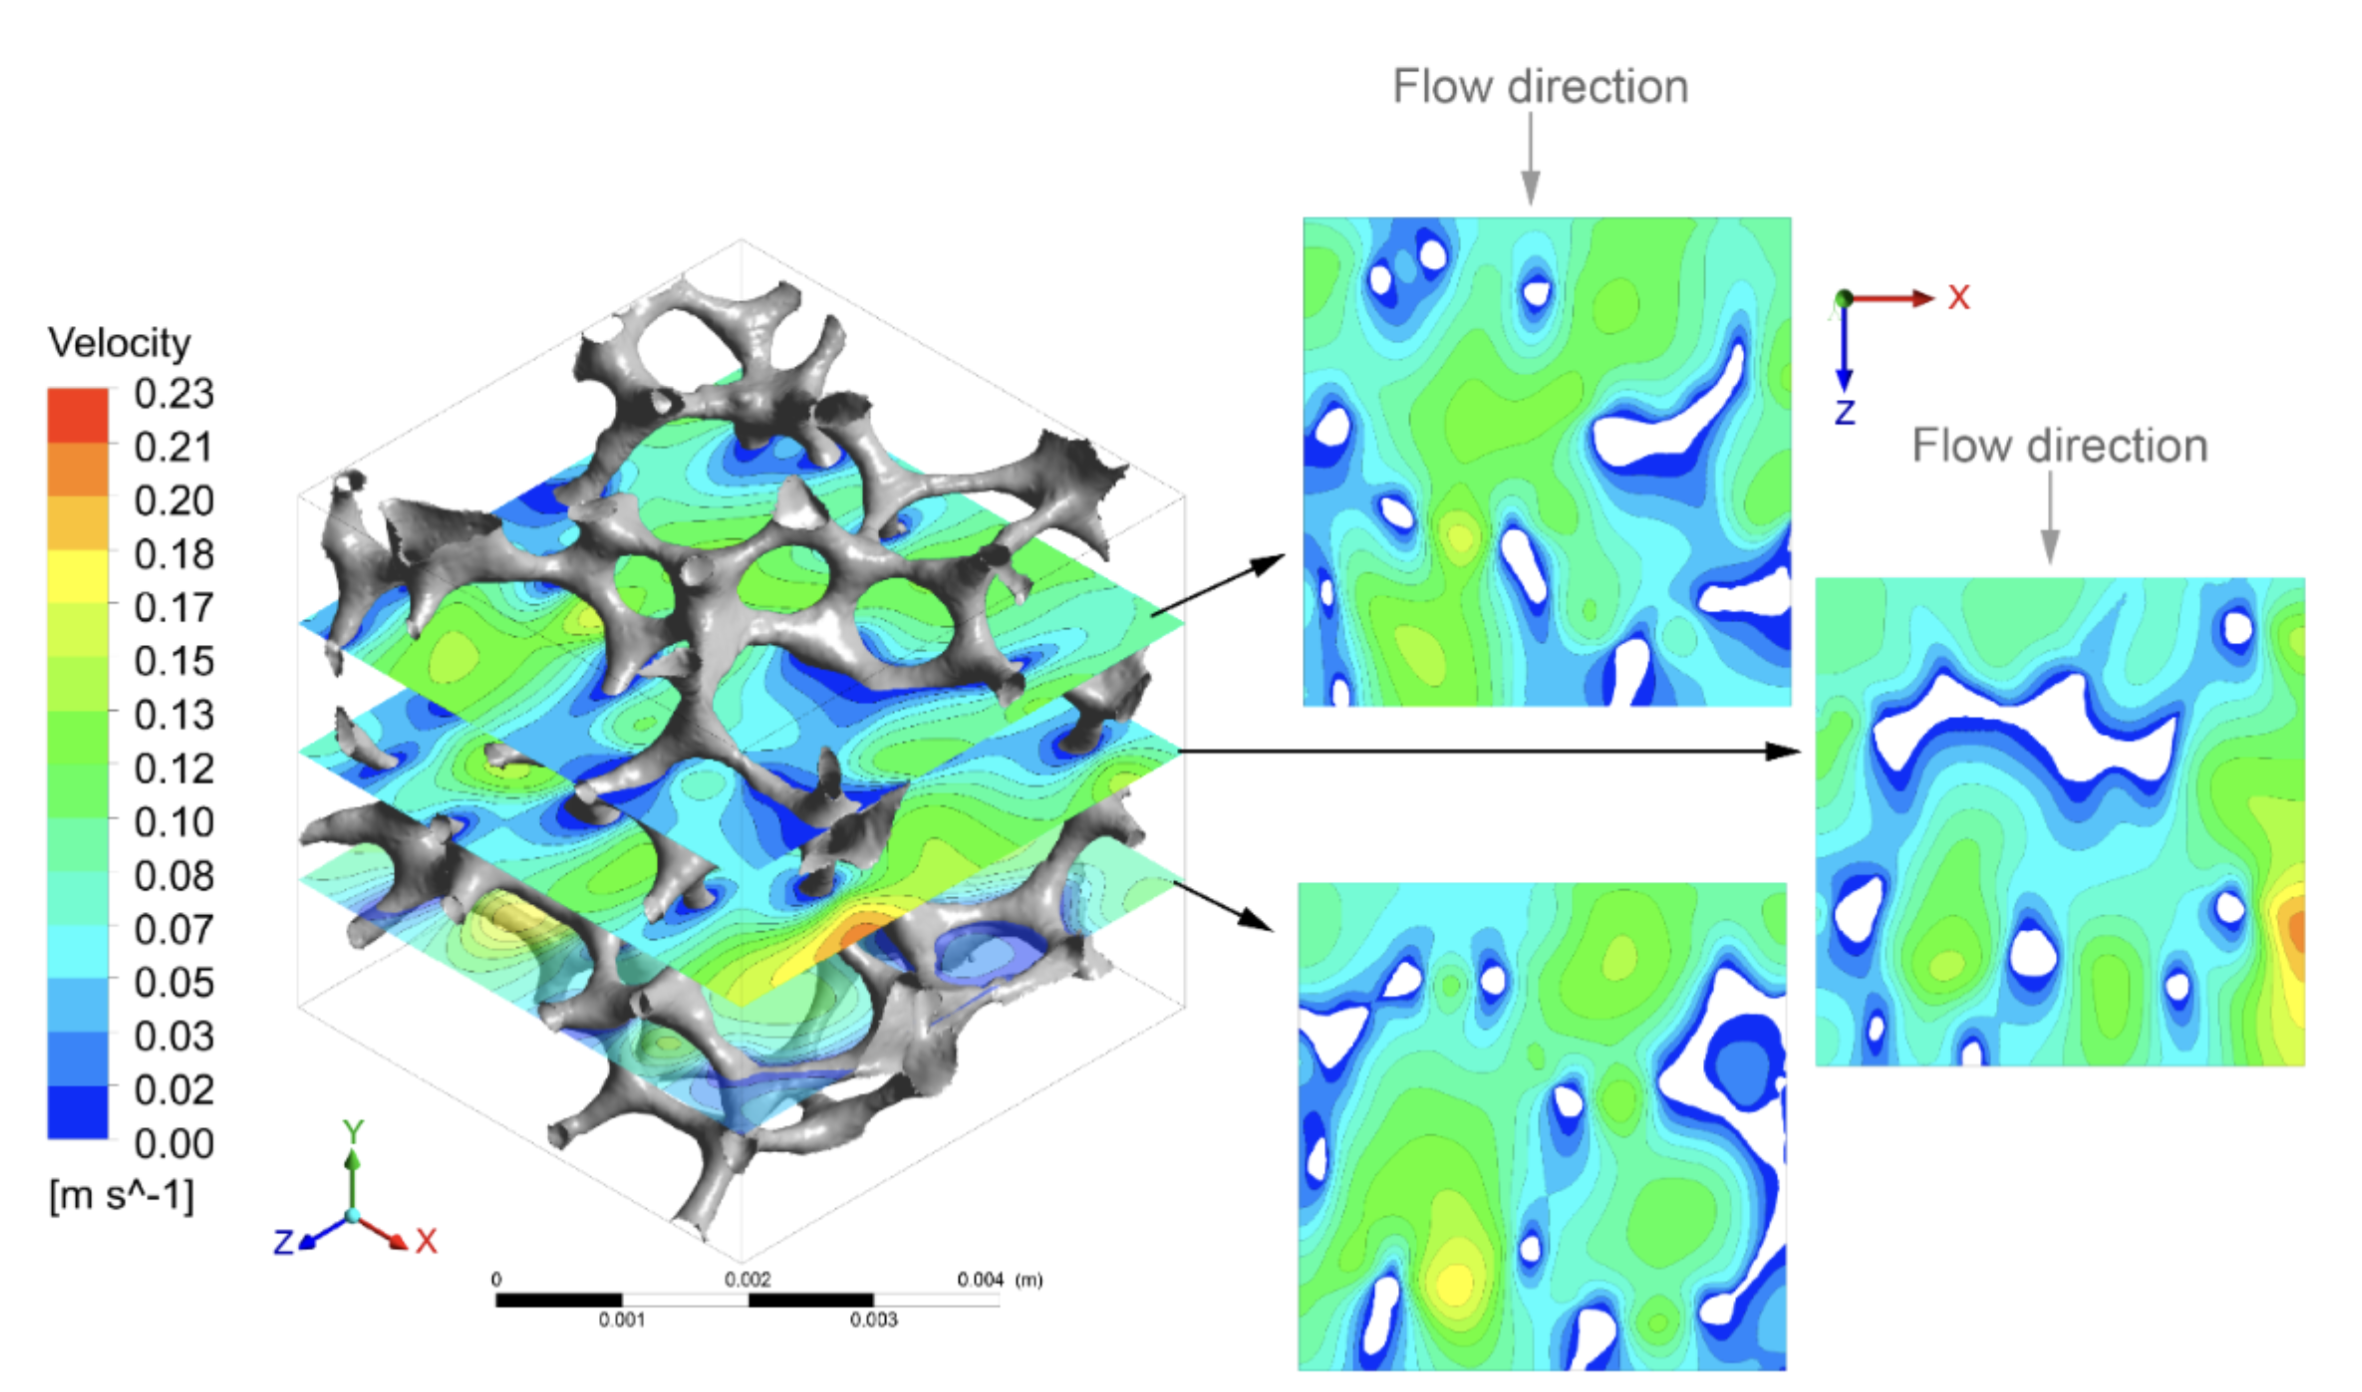
\includegraphics[width=12cm]{vysledky_CFD_CT.png}
  \centering
  \caption{Visualization of the resulting velocity contours inside the 30 PPI foam \cite{Ranut2014}.}
\end{figure}


\pagebreak

\part{Numerical and Experimental Investigation}
The second part of this dissertation presents the original research carried out within the framework of this doctoral project. The research combines experimental measurements with advanced numerical simulations to investigate the hydraulic and thermal behaviour of porous material based cooling channels intended for high heat flux applications in future nuclear fusion devices.
\\
\\
The study follows a progressive methodology in which individual research tasks build upon one another. The investigation begins with the development and description of the experimental infrastructure, including the TEALC experimental facility and the induction heating system designed to reproduce representative thermal loading conditions. This facility provides the basis for both hydraulic measurements and future high heat flux experiments.
\\
\\
To support the interpretation of experimental data, extensive computational fluid dynamics (CFD) simulations were performed. First, simplified substitute geometries were developed to evaluate the influence of characteristic porous structure parameters on pressure losses and hydraulic performance. The numerical methodology was validated through mesh sensitivity analyses and comparison with experimental measurements. Subsequently, realistic porous structures reconstructed from micro-computed tomography scans were employed to investigate both hydraulic characteristics and conjugate heat transfer within the porous media.
\\
\\
The experimental programme includes the characterization of several porous samples with different structural parameters, providing quantitative information about permeability, pressure drop and flow resistance. These data are subsequently used to validate the numerical models and to establish reliable correlations for engineering design.
\\
\\
The final stage of the research focuses on proof-of-concept experiments investigating porous material cooling channels under high heat flux conditions approaching the critical heat flux regime. The obtained results are evaluated with respect to their applicability for plasma-facing components in future fusion reactors and are compared with conventional cooling technologies discussed in the theoretical part.
\\
\\
Together, the presented experimental and numerical investigations provide a comprehensive assessment of porous material based cooling channels and demonstrate their potential as an alternative high-performance cooling technology for future magnetic confinement fusion devices.

\pagebreak
\section{Basic Research}
The preliminary research undertaken before the main porous-channel programme established the experimental and numerical methods required for high-heat-flux testing. It included assessment of available heat sources, development of induction-heating methodology, numerical investigation of hypervapotron cooling and an experimental study of boiling behaviour using the Leidenfrost configuration.

Several options are available for researchers to recreate the thermal conditions encountered by plasma-facing components.
In order to use a heating source for the high heat flux cooling channels testing, heating source should in an ideal case meet those conditions:
\begin{enumerate}
  \item Heating power and surface heat flux uniformity is known.
  \item Source can provide heat flux density in magnitude expectable in fusion devices ($\geq$10~MW/m$^2$).
  \item Heating can be sustained for a sufficient amout of time.
  \item Area of provided heat flux (size of the tested samples) is large enough, to observe fully developed coolant flow effects.
\end{enumerate}

\noindent Heating sources commonly used for high heat flux cooling experimental research:
\begin{itemize}
  \item Ohmic heating.
  \item Induction heating.
  \item Laser beam.
  \item Plasma torch.
  \item Chemical reactions.
\end{itemize}

\noindent Ohmic heating provides uniform heat generation through electrical resistance in a conductor, achieving high heat flux densities but typically requires careful control to ensure sustained and uniform power delivery. 
The biggest advantage of ohmic heating is easily obtained heating power measurement. 
However, the heating conductor needs to be attached to the examined FW sample - volumetric heating sources in general are not able to provide temperature profiles comparable with radiative load in the fusion reactor.
Electromagnetic induction can provide heating power to samples without any mechanical contact - a practical way to examine a large number of samples, though it may be limited in its heating uniformity and material requirements. 
Metal alloys used in fusion reactor construction are usually not very efficient for inductive heating (a combination of electrical conductivity and magnetic permeability), therefore the sample material composition needs to be adjusted.
Induction heating allows the attachment of thermocouples to the tested samples from multiple directions.
Non-uniformity of volumetric heating is one of the most significant disadvantages of electromagnetic induction heating.
\\
\\
\noindent Laser beams deliver focused, high-intensity heat with excellent precision and the capability to achieve very high heat flux densities, but their application over large areas and sustained heating can be challenging. High-power laser and electron-beam facilities additionally require specialised and comparatively expensive infrastructure, which limits their accessibility for iterative laboratory testing. 
In general: the laser beam provides both control over the uniformity of heat flux, fast changes of heat load simulating the plasma-wall interaction and the source creates temperature profiles similar to the real plasma load, but they are usually very strictly limited by the total power output - allowing only small-sized experimental samples.
Plasma torches can achieve extremely high temperatures and heat flux densities with broad area coverage, but the total heating power and load uniformity is very questionable. 
Chemical exothermic reactions can also provide heat, but achieving uniform distribution and controlling the reaction over extended periods can be problematic. 
Chemical reaction of thermite (considered to be extremely exothermic) can provide the heat flux only up to 0.1~MW/m$^2$ below the desired range of fusion reactor conditions and also for a very limited period of time \cite{DS23}.

\pagebreak
\noindent The article describes both the simulation and the experimental research performed on HEFEL experimental loop, built to study the hypervapotron subcooled boiling. 
One of the biggest challenges in performing the experimental research was: reaching the heat fluxes where the subcooled boiling occurs and precisely measuring the heat flux value.
The electromagnetic induction heating is simulated in ANSYS Maxwell 3D and coupled with ANSYS Fluent to simulate the heat transfer behaviour and extract the temperature profiles. 
Experiments validated the numerical models by the resistance thermometers inserted into the solid samples to monitor temperature. A significant result is the increase in heat flux with the use of steel sheets in the CuCrZr body, achieving a maximum solid temperature of 1057°C, though the target flux of 10~MW/m$^2$ was not fully reached.
the schematic of performed work is shown in Figure \ref{fig:indukce}.
\begin{figure}[h]
  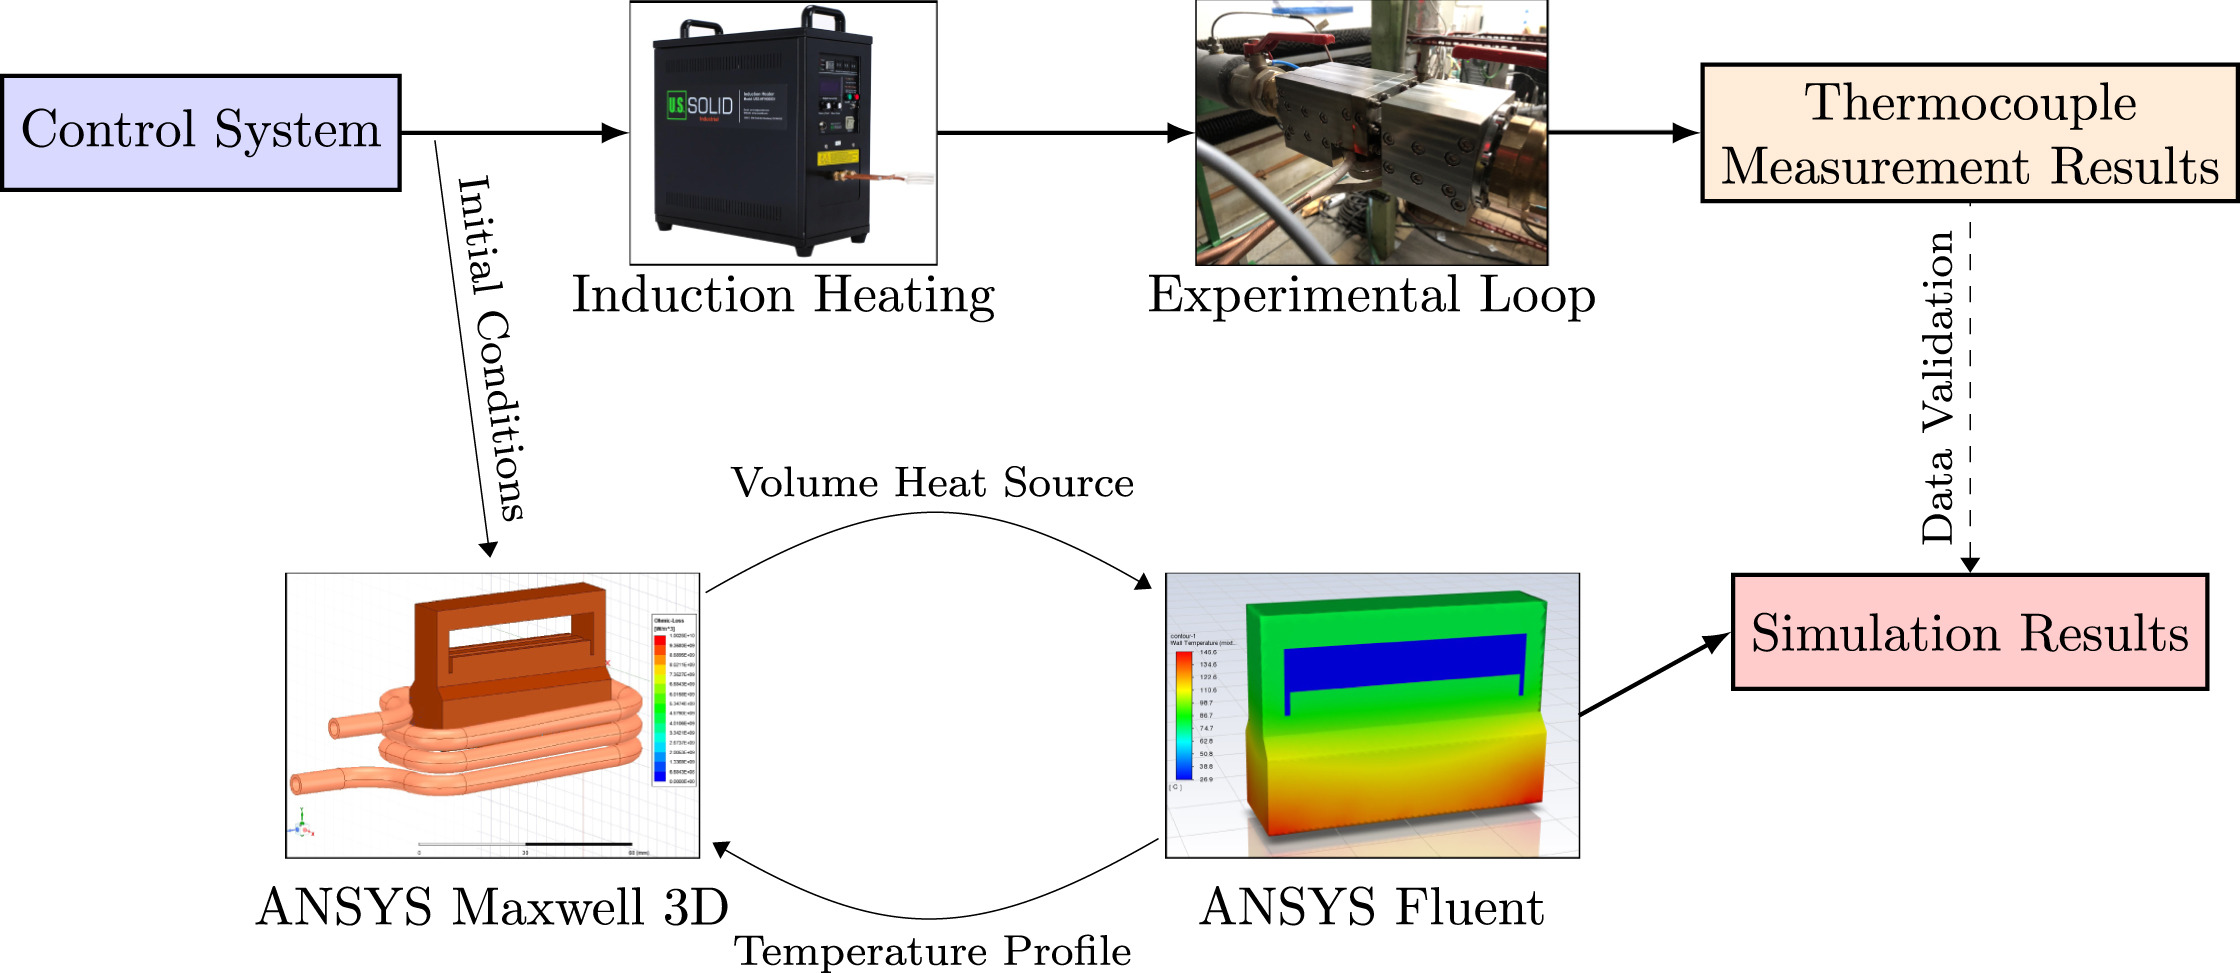
\includegraphics[width=14cm]{schema_indukce.jpg}
  \centering
  \caption{Experimental and numerical setup \cite{S2023}.}
  \label{fig:indukce}
\end{figure}
\noindent One of the key challenges in this setup is the choice of materials, as the low relative permeability of CuCrZr limits the efficiency of induction heating. To overcome this, steel sheets were added to increase the heating power, though overheating and disruptions in the temperature profile occurred. These findings highlight the importance of optimizing material properties and geometry for better heat transfer. 
\\
\\
Overall, the induction heating method proved to be a viable alternative to conventional heating techniques, providing valuable insights into heat transfer behaviors for high heat flux applications. 
The experimental validation of the numerical models supports future optimization of heated samples and it also is a very useful tool to estimate the generated heating power.
The same heating source and methodology were subsequently applied to the porous-copper cooling-channel study \mycite{Smolk2024}.

\pagebreak

\subsection{Numerical research of the hypervapotron}
Subcooled boiling represents a challenging task for both experimental and numerical studies.
From the experimental point of view, the hypervapotron effect is reached only at high heat fluxes and the examination of long sections of the channel is needed to observe the fully developed hypervapotron effect, thus a heating source with high power output is needed.
Researchers usually decrease the operating pressure of cooling water, or substitute the cooling medium to one with the boiling temperature significantly lower than water to observe the hypervapotron effect on lower range of heat fluxes.
The numerical simulations of the subcooled boiling regime are a very challenging task for the recent computational resources.
In general, the boiling regime can be simulated by two different approaches: a VOF (volume of fluid) model considering two phases (liquid water a vapour), assigning each mesh cell a certain value of volume fraction of those two phases.
Another approach is the Eulerian model, simulating each vapour bubble as a separate domain. 

\begin{figure}[h]
  \centering
  \begin{minipage}{0.45\textwidth}
      \centering
      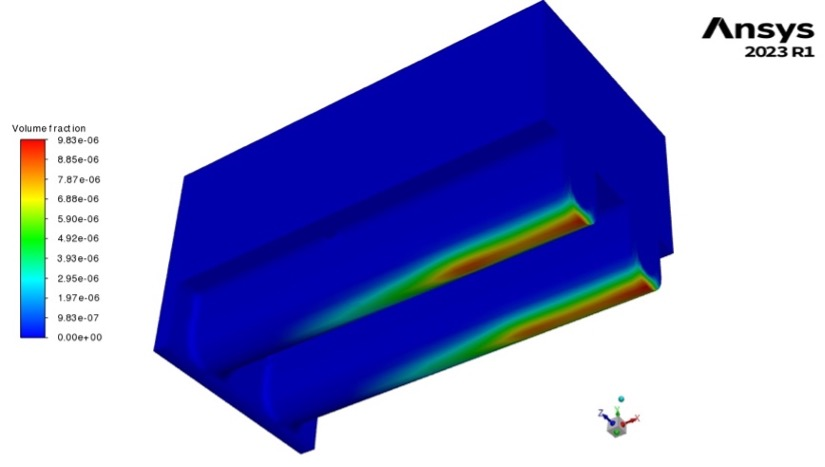
\includegraphics[width=\linewidth]{hypervapo_vys2.jpg}
  \end{minipage}\hfill
  \begin{minipage}{0.4\textwidth}
      \centering
      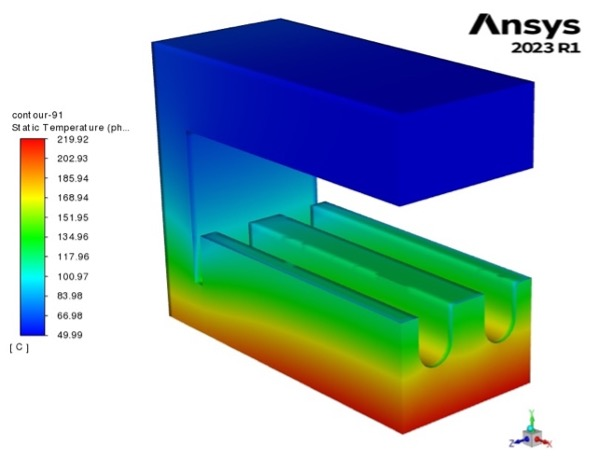
\includegraphics[width=\linewidth]{hypervapo_vys1.jpg}
  \end{minipage}
  \caption{Numerical results: vapour volume fraction profile (left) and temperature profile (right), heat flux 4~MW/m$^2$, inlet water: 50 °C, 6~bar, 4~m/s \cite{Smolk2023}.}
  \label{fig:hypervapotron3}
\end{figure}

\noindent Figure \ref{fig:hypervapotron3} shows an example of CFD simulation of the hypervapotron using ANSYS Fluent 23.1 software and the Eulerian model settings.
The resulting vapour volume ratio in the fluid domain (left) and the corresponding CuCrZr solid temperature profile is shown.
There is only a limited number of available experimental data (operating in the first wall cooling relevant range of conditions) to validate the numerical models.
Figure \ref{fig:hypervapotron4} shows the comparison of various CFD solvers for the same case of hypervapotron subcooled boiling at variable heat flux conditions and the experimental data for validation.
The latest calculation performed in ANSYS Fluent 23.1 successfully simulated how the vapour bubbles join to create a continuous layer of vapour, insulating the incoming heat flux and resulting in the boiling crisis (the critical heat flux, CHF).
\begin{figure}[h]
  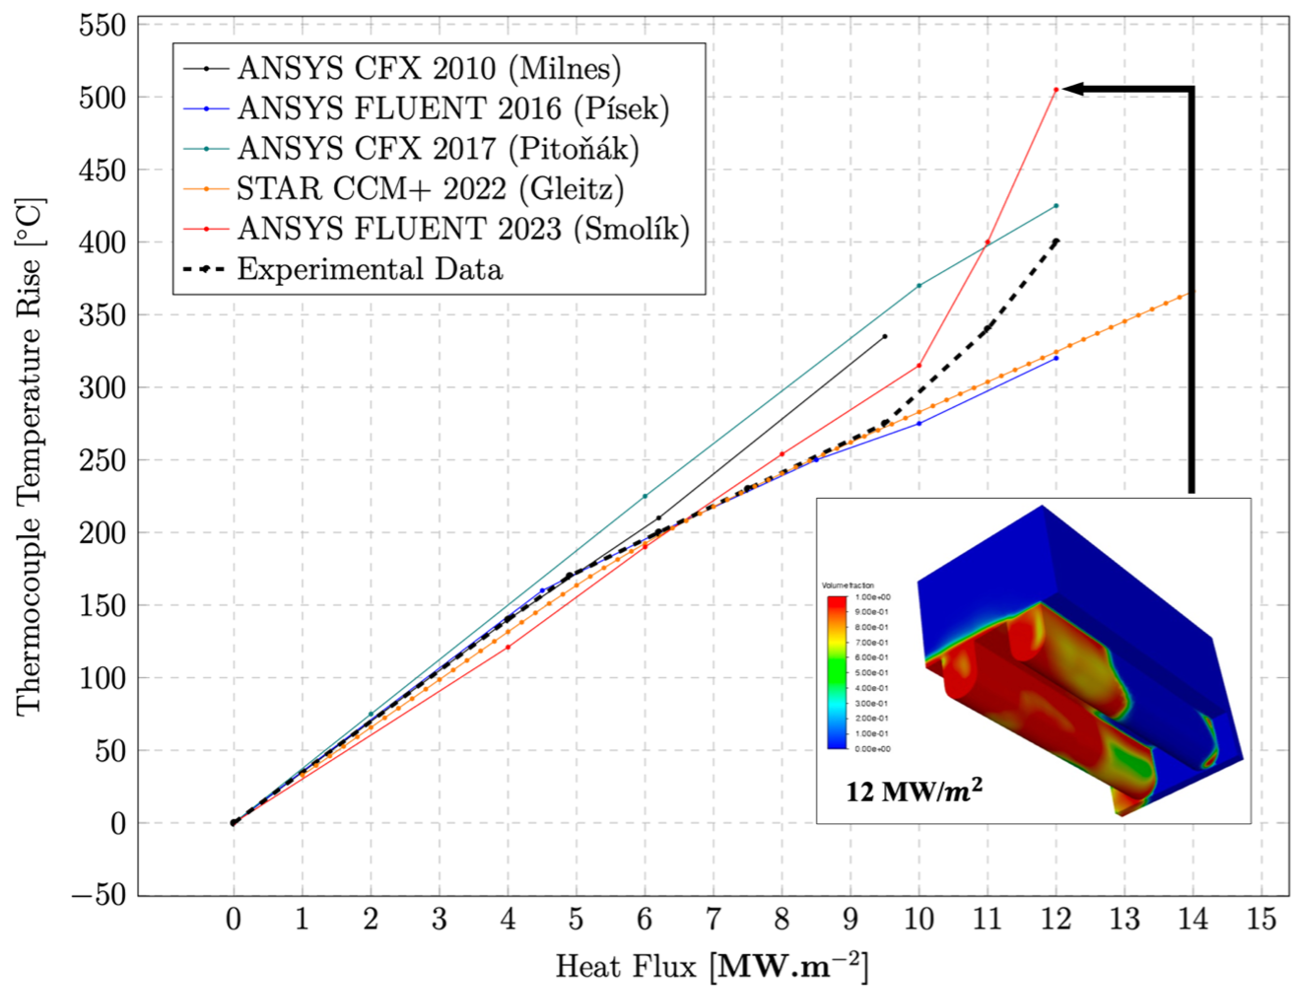
\includegraphics[width=11cm]{hypervapo_vysledky.png}
  \centering
  \caption{ Experimental and numerical results, variable heat flux, inlet water: 50 °C, 6~bar, 4~m/s \cite{Smolk2023}. Experimental validation data taken from Ciric \cite{Ciric}.}
  \label{fig:hypervapotron4}
\end{figure}

\pagebreak

\subsection{Experimental research of the Nukiyama curve}

An experimental study was performed to observe and describe if the Nukiyama curve (defined for the pool boiling) is also present in the case of a single drop boiling on a hot surface - the Leidenfrost effect.
Figure \ref{fig:leid1} shows the similar presence of the insulating vapour layer in both the Leidenfrost effect (a) and the boiling crisis (b) \cite{LEIDENFROST19661153}.

\begin{figure}[h]
  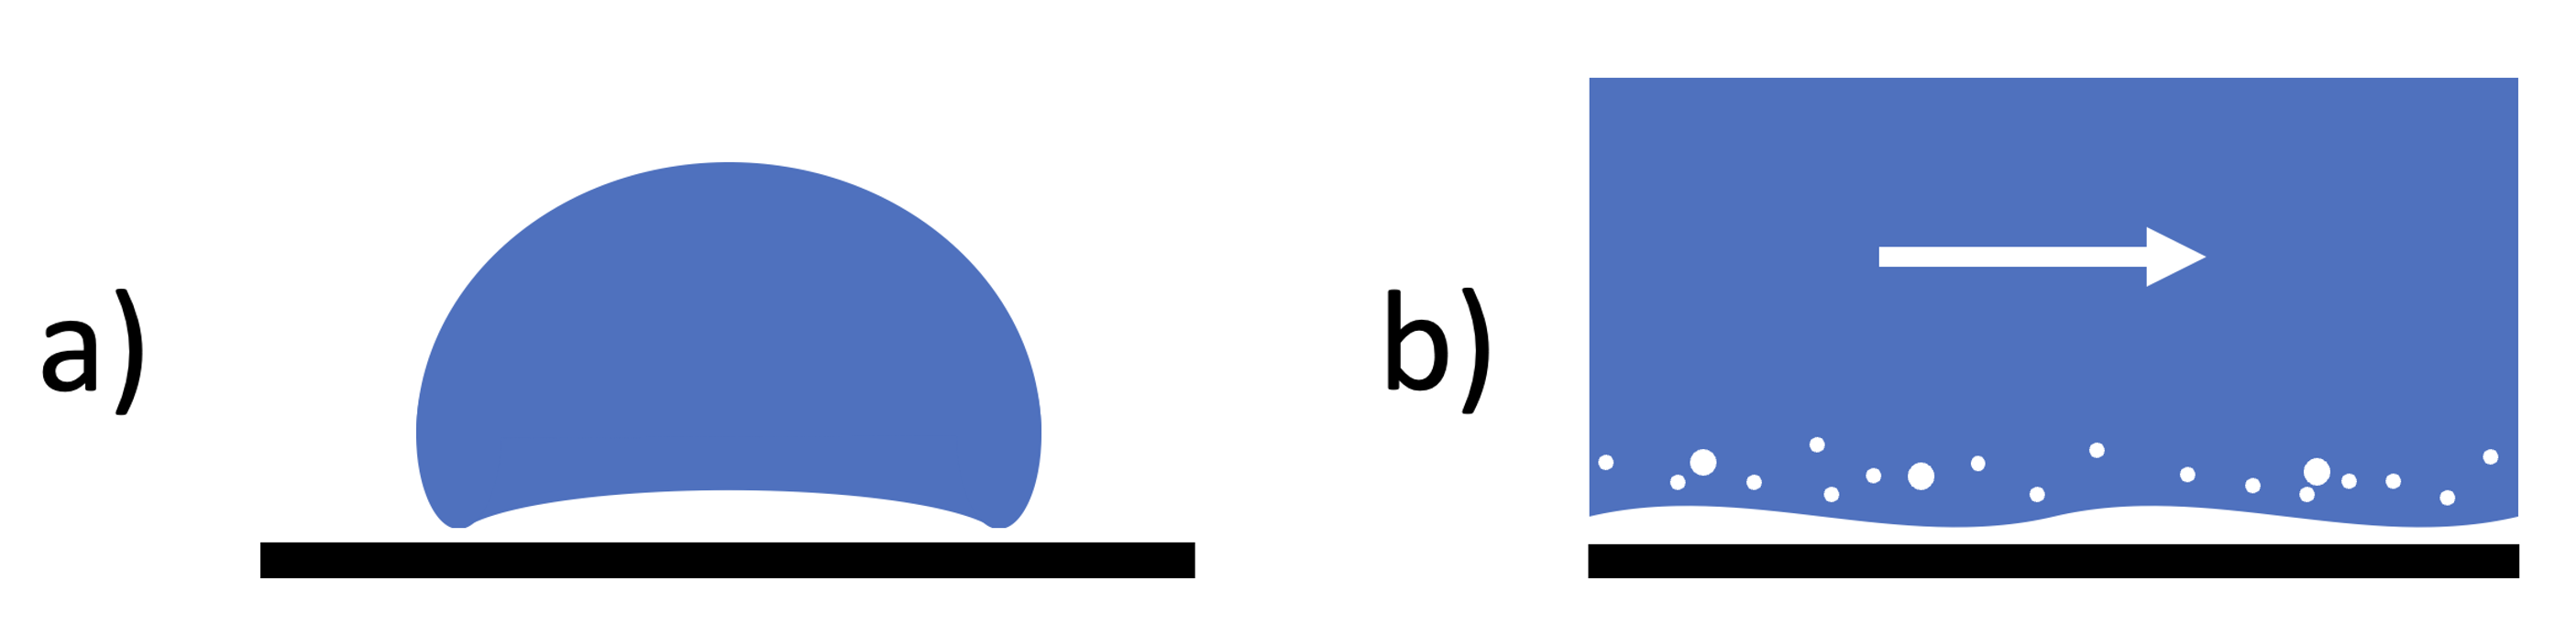
\includegraphics[width=8cm]{porovnani_kapky.png}
  \centering
  \caption{a) the Leidenfrost effect b) boiling crisis in cooling channel \cite{Smolik2025} }
  \label{fig:leid1}
\end{figure}

\noindent A steel monoblock is heated up by the induction heating source coil, thermocouple B helps to control the temperature of the heated sample.
Another thermocouple A is installed on the copper surface of the experimental sample to accurately measure the surface temperature of wall nearby water droplets.
Camera captures the deposition and evaporation of water droplets, the volume of droplets is controlled by a calibrated FINNPIPETTE F2 10-100 $\mu$l pipette.
Induction heating allows to reach controlled temperatures up to 400~$^\circ$C.

\begin{equation}
  q= \dfrac{E_v}{t_{avg} \cdot A_{drop}}
  \label{eq:leid1}
\end{equation}

\noindent Equation \ref{eq:leid1} shows how the measured evaporation time $t_{avg}$ was used in relation to the total evaporation energy $E_v$ and area under the water droplet $A_k$ to calculate the resulting heat flux $q$.
In order to simplify the calculation method, the droplet shape was simplified to a hemisphere with the same volume as the droplet and the contact area of this hemisphere remains constant during the whole process of evaporation.
Those simplifications can be implemented, since the overall shape of the resulting boiling curve is the research focus, not the absolute values.

\begin{figure}[h]
  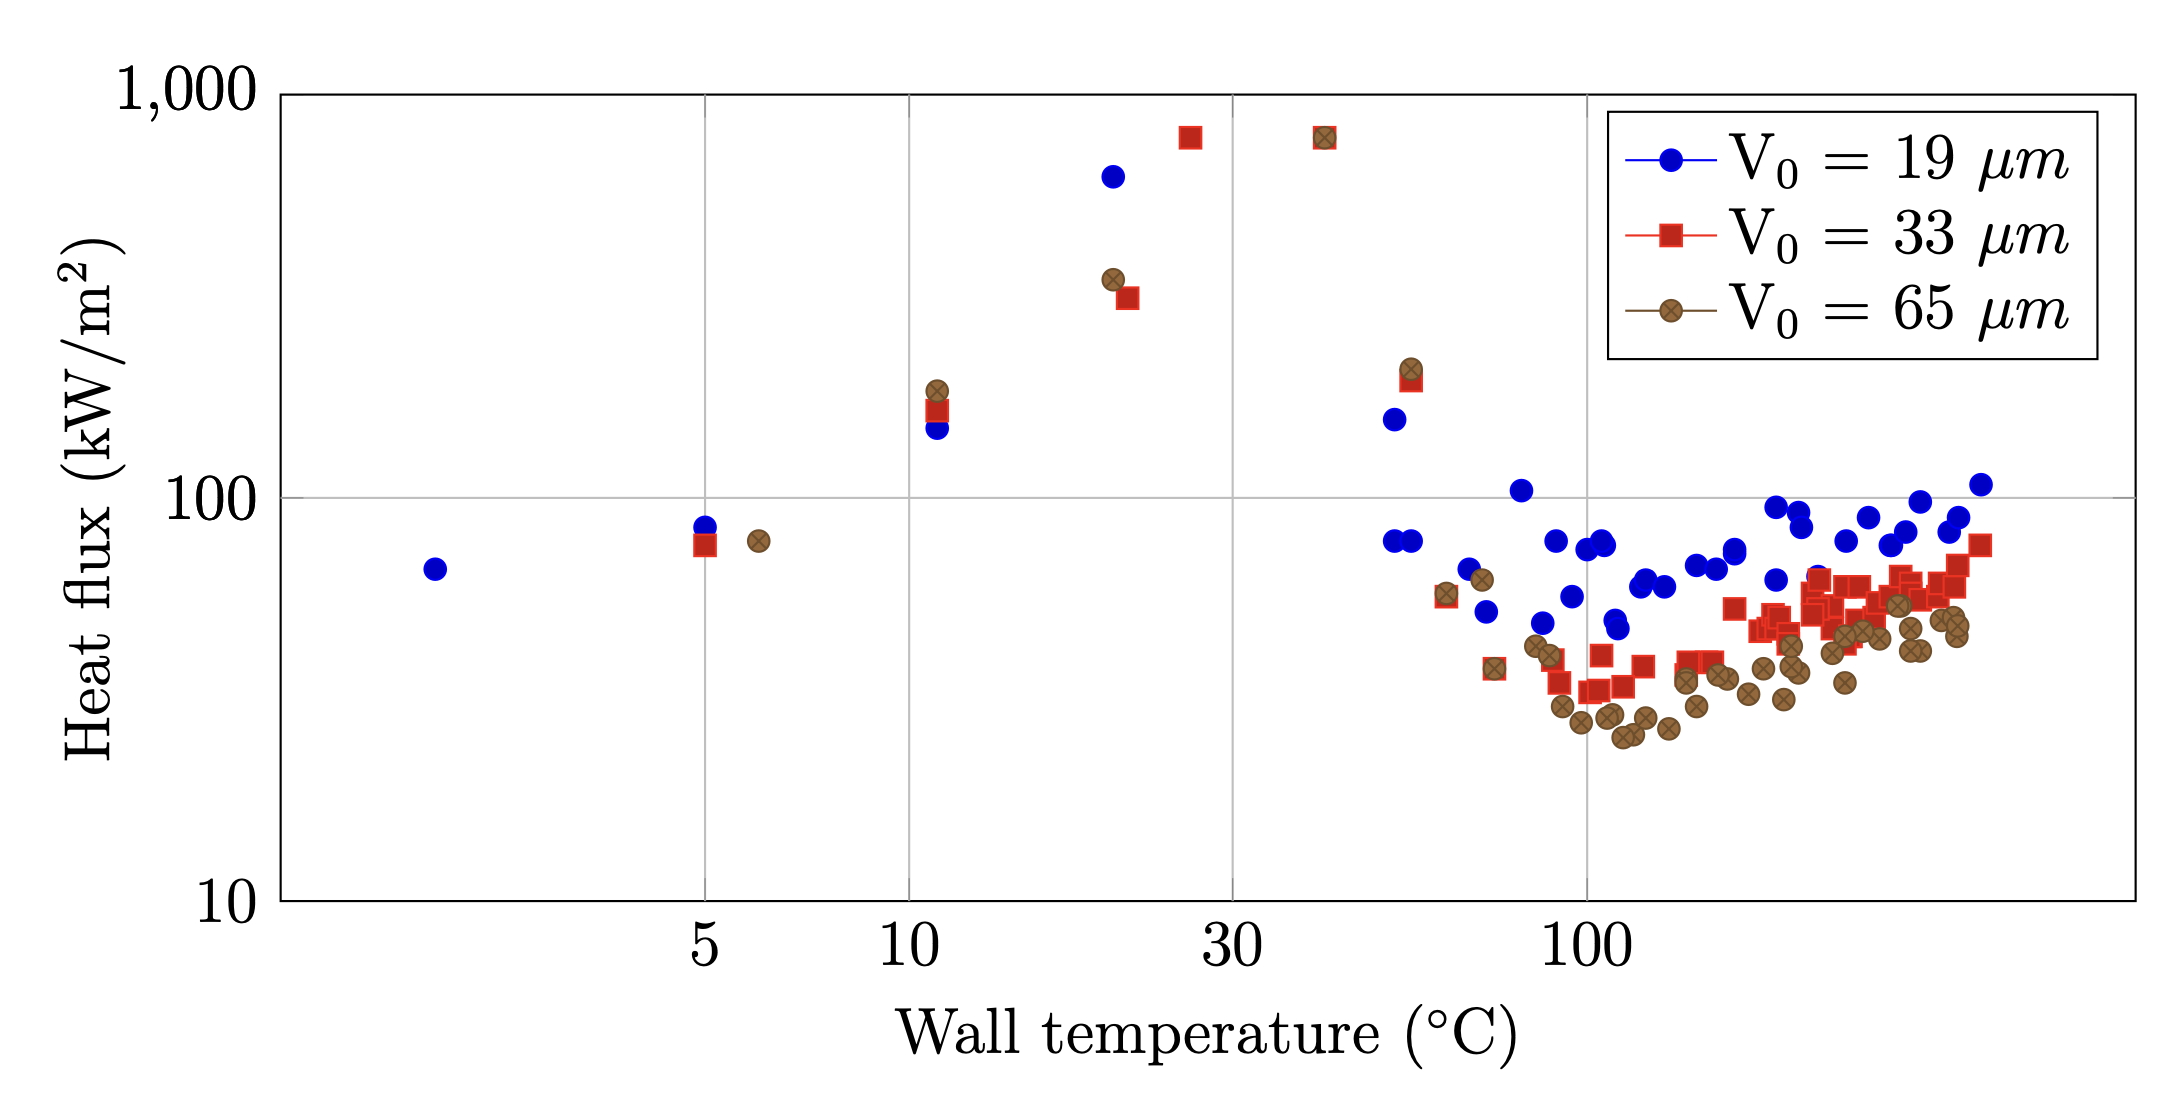
\includegraphics[width=12cm]{nukiyama_vlastni.png}
  \centering
  \caption{Nukiyama boiling curve observed on the Leidenfrost effect \cite{Smolik2025}.}
  \label{fig:leid3}
\end{figure}

\noindent Figure \ref{fig:leid3} shows a very strong agreement with the previously mentioned Figure \ref{fig:nuk}. 
Thanks to the induction heating source, the surface wall temperature was measured up to 390~$^\circ$C.
All the regions of Nukiyama curve are clearly observable. 
Maximum in the point of critical heat flux $q_{maxi}$ at 30~$^\circ$C and the minimum at 
An increase in heat flux for temperatures above the Leidenfrost point (approx. 120~$^\circ$C) is observable.

\pagebreak

\section{The use of substitute geometries and accuracy of CFD}
To evaluate the ability of CFD to predict the pressure drop in microstructure porous materials, a numerical study was conducted using ANSYS Fluent 2023.1.
The workflow of this study was to build a parametric model of periodic microstructure with variable dimensions and evaluate both the pressure drop and the flow velocity distribution in the porous zone.
Selected geometry parameters were porosity and tortuosity, which are the most significant parameters affecting the viscous behavior of porous materials.
The goal of the validated numerical model is to evaluate the relation between tortuosity, porosity and pressure drop coefficients (permeability and Forchheimer coefficient) in the porous zone and to provide a tool for the design of high heat flux cooling channels based on porous materials.
A high resolution 3D printing was used to create the physical samples of the porous microstructure, which were then tested in the TEALC experimental loop to validate the numerical model.

\subsection{Parameter 1 - Porosity}
Porosity was previously defined as the ratio of the volume of voids to the total volume of the porous material, expressed by Equation 9.
A set of geometries with different porosity values was created to evaluate the effect of porosity on the pressure drop in the porous zone.
Figure \ref{fig:grid_cfd_2} shows the 8x8x8 mm sample of the porous microstructure with a variable porosity ranging from 4.3 up to 95.4~\%, which was used for the CFD analysis.
\begin{figure}[h]
  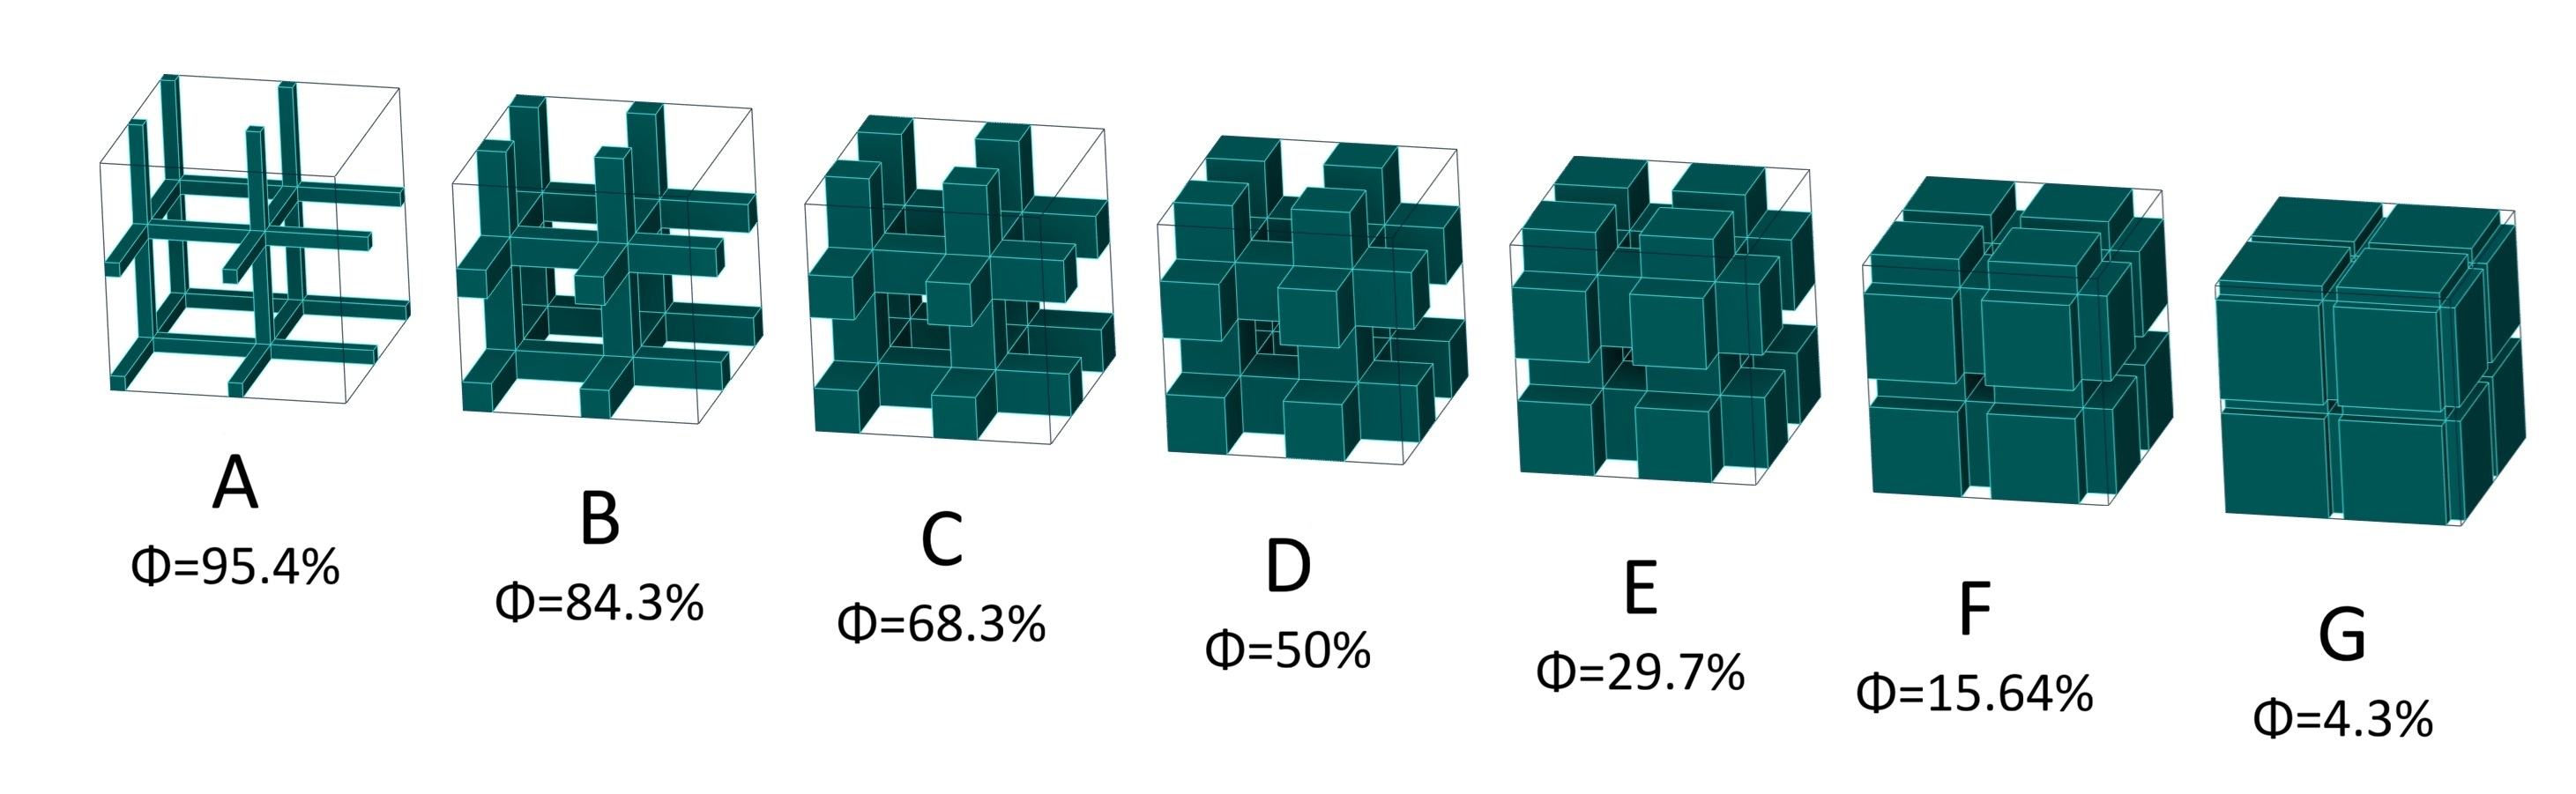
\includegraphics[width=12cm]{grid_cfd_2.jpg}
  \centering
  \caption{Geometry with variable porosity used for CFD analysis.}
  \label{fig:grid_cfd_2}
\end{figure}

\subsection{Parameter 2 - Tortuosity}
Figure \ref{fig:grid_cfd_3} shows the 8x8x8 mm sample of the porous microstructure with a variable tortuosity ranging from 1.0 up to 2.0, which was used for the CFD analysis.
The tortuosity parameter was defined as the ratio of the actual flow path length to the straight-line distance between the inlet and outlet of the porous zone, expressed by Equation 11, also illustrated in Figure 46.
\begin{figure}[h]
  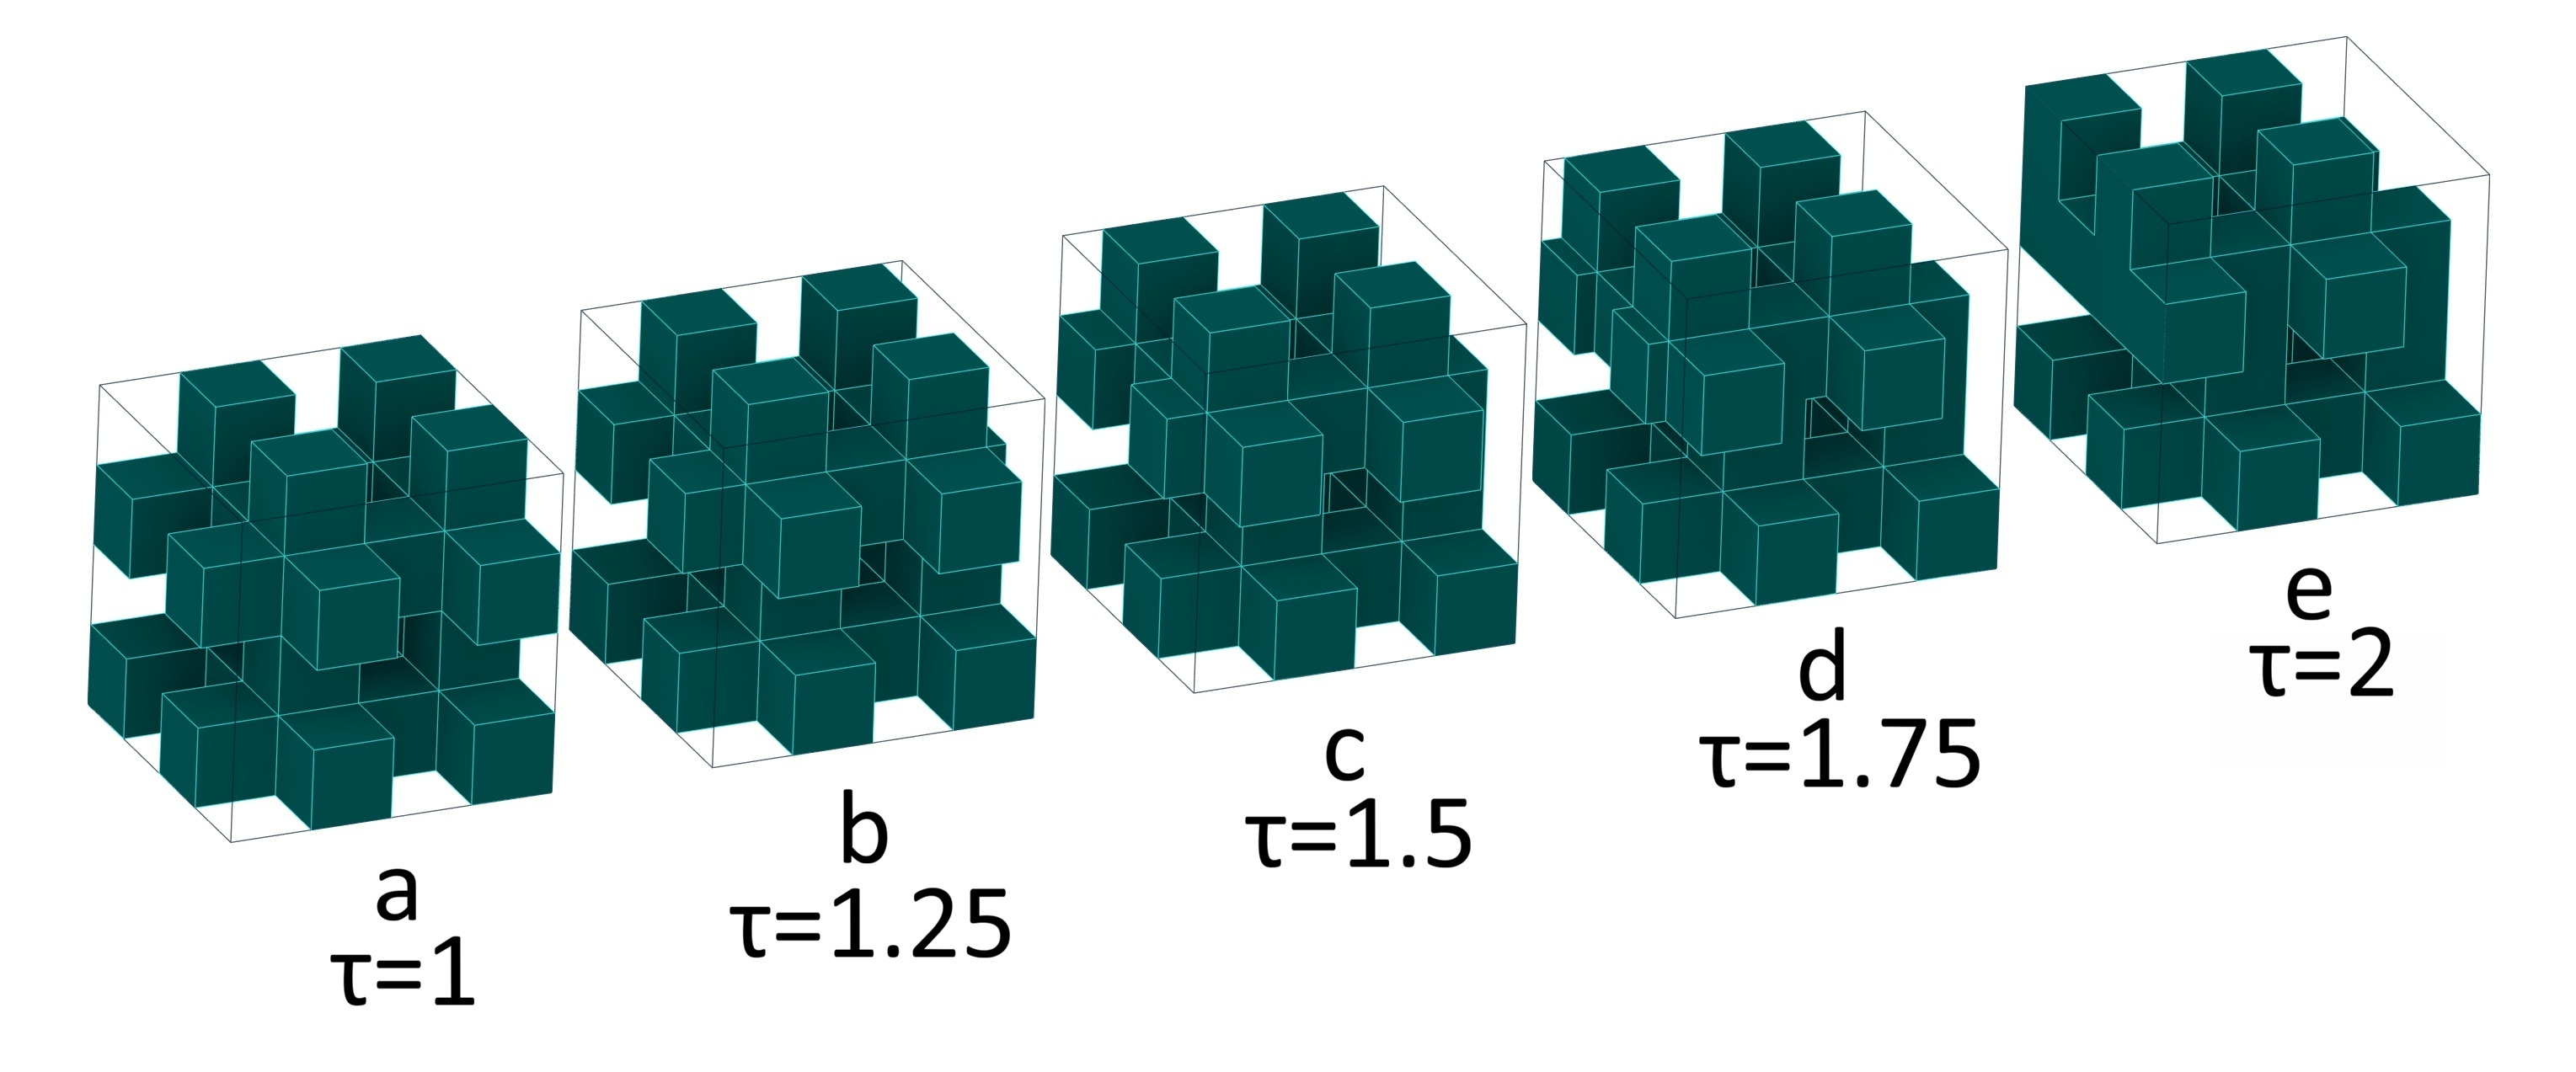
\includegraphics[width=10cm]{grid_cfd_3.jpg}
  \centering
  \caption{Geometry with variable tortuosity used for CFD analysis.}
  \label{fig:grid_cfd_3}
\end{figure}


\pagebreak
\subsection{An overview of used geometries}
Table 4 provides an overview of the sample geometries used in the CFD analysis, which were designed with varying porosity and tortuosity values.
Total number of samples is 35, with 5 different tortuosity values and 7 different porosity values.
Samples marked with an asterisk (*) were selected for the experimental validation of the numerical model in the TEALC experimental loop.
\begin{table}[h!]
\centering
\begin{tabular}{c|ccccccc}
\hline
Tortuosity & \multicolumn{7}{c}{Porosity $\Phi$} \\
\hline
 & 0.954 & 0.843 & 0.683 & 0.500 & 0.297 & 0.156 & 0.043 \\
\hline
1.00 &Aa &\textbf{Ba}$^{\mathbf{*}}$ &Ca &\textbf{Da}$^{\mathbf{*}}$ &Ea &Fa &Ga \\
1.25 &Ab &Bb &Cb &Db &Eb &Fb &Gb \\
1.50 &Ac &Bc &Cc &Dc &Ec &Fc &Gc \\
1.75 &Ad &Bd &Cd &Dd &Ed &Fd &Gd \\
2.00 &Ae &Be &Ce &De &Ee &Fe &Ge \\
\hline
\end{tabular}
\label{tab:porosity_tortuosity_samples}
\caption{Overview of sample geometries with different porosity and tortuosity values.}
\end{table}

\subsection{CFD analysis setup}
Figure \ref{fig:grid_cfd_setup} shows the CFD analysis setup. The 40 mm porous sample is inserted into a 16x24 mm channel, with a 100 mm inlet and outlet length to ensure fully developed flow conditions.
The inlet boundary condition is set as a velocity inlet, while the outlet is defined as a pressure outlet. The walls of the channel are treated as no-slip boundaries.
The fluid used in the simulation is water at room temperature, with properties defined according to standard conditions.

\begin{figure}[h]
  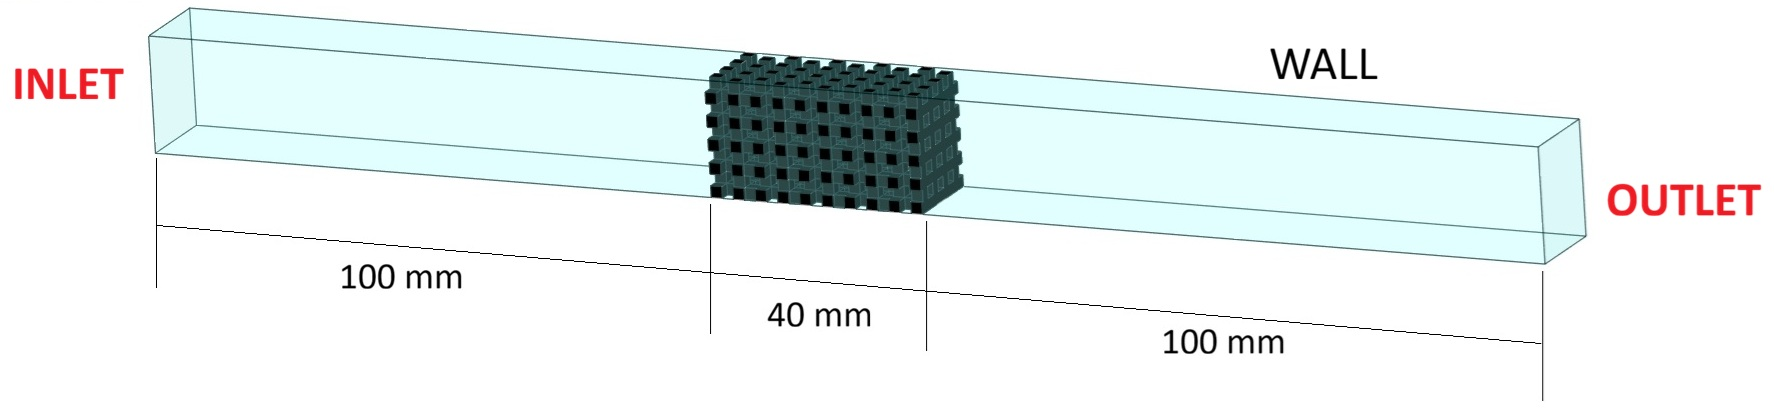
\includegraphics[width=14cm]{grid_cfd_1.jpg}
  \centering
  \caption{CFD analysis setup.}
  \label{fig:grid_cfd_setup}
\end{figure}

The dimensions of the computational domain were selected as a compromise between numerical accuracy and computational efficiency. The periodic porous structure was modelled over a sufficiently long distance to ensure that the flow within the sample was fully developed and unaffected by the inlet and outlet boundary conditions or by the influence of the surrounding channel walls. At the same time, the computational domain was intentionally kept as small as possible to limit the overall number of computational cells and maintain reasonable simulation times without compromising the accuracy of the predicted hydraulic characteristics.
\pagebreak

\subsubsection{CFD model and viscous settings}
The numerical simulations were performed using \textit{ANSYS Fluent 2025 R2}. Water was selected as the working fluid, with its thermophysical properties taken from the built-in Fluent material database. The flow was assumed to be incompressible, single-phase and steady-state. A pressure-based solver was employed, which represents the standard solution approach for incompressible internal flows. Pressure--velocity coupling was achieved using the SIMPLE algorithm, while second-order spatial discretization schemes were applied to all governing equations in order to improve numerical accuracy and reduce numerical diffusion. Solution convergence was assessed by monitoring the residuals of the governing equations together with the stabilization of integral quantities, particularly the pressure drop across the computational domain.
\\
\\
Turbulence effects were modelled using the Shear Stress Transport (SST) $k$--$\omega$ model, which is the default turbulence model in ANSYS Fluent for a broad range of engineering applications involving wall-bounded flows. The SST formulation combines the near-wall accuracy of the standard $k$--$\omega$ model with the robustness of the $k$--$\varepsilon$ model in the free-stream region through a blending function. This approach provides reliable predictions of velocity profiles, wall shear stresses and pressure losses, especially in flows with separation or adverse pressure gradients. Unless stated otherwise, the default model constants and solver settings provided by ANSYS Fluent 2025 R2 were retained throughout all simulations to ensure a consistent numerical methodology across the investigated cases.
\\
\\
Gravity was enabled throughout all simulations and oriented perpendicular to the principal flow direction, corresponding to the orientation of the experimental facility. Although the investigated flow velocities resulted in Reynolds numbers for which inertial effects dominated over buoyancy, the gravitational body force was retained to reproduce the experimental configuration as closely as possible. No significant influence of gravity on the predicted pressure losses was observed.
\\
\\
No-slip boundary conditions were applied to all solid walls, including both the channel walls and the surfaces of the porous structure. Since the SST $k$--$\omega$ model provides an integrated near-wall treatment, no additional wall functions or modified near-wall models were required. The near-wall mesh resolution was therefore selected to satisfy the requirements of the turbulence model during the subsequent mesh independence study.
Each simulation was continued until both the residuals of all governing equations and the monitored pressure drop reached stable values. In addition to the residual history, the convergence of the pressure loss across the porous sample was used as the principal engineering criterion, since it represents the primary quantity evaluated in this study.



\newpage
\subsection{Mesh sensitivity analysis}
A mesh sensitivity analysis was performed to evaluate the impact of mesh refinement on the simulation results. 
The flow patterns inside the porous structure are complex, and the mesh needs to be sufficiently refined to capture the flow behavior accurately.
The geometry variant \textbf{De} was selected for the mesh sensitivity analysis, with a porosity of 0.500 and a tortuosity of 2, because it represents a case with many flow obstructions and a complex flow path.
\\
\\
Because different geometry cases have different fluid volume, the total number of cells cannot be compared across the different geometry cases, it serves only as a measure to evaluate the mesh refinement for a specific geometry case.
The wall inflation settings were set to uniform, 6 layers with a growth rate of 1.2, and the first layer thickness was set to 0.01 mm.
The inflation settings prevented issues with variable first layer thickness in the region of the entrance to the porous zone, which could lead to numerical instabilities and convergence issues.
Figures \ref{fig:grid_mesh_prehled} show a detailed look at some of the generated mesh for the C

\begin{figure}[h]
    \centering

    \begin{subfigure}[t]{0.32\textwidth}
        \centering
        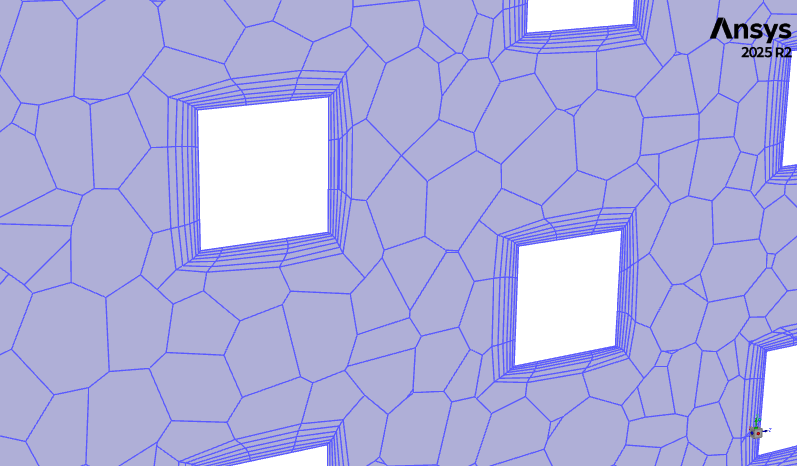
\includegraphics[
            width=\linewidth,
            trim={0 0 7cm 0},
            clip
        ]{gridmesh_B.png}
        \caption{250k cells mesh}
        \label{fig:grid_mesh_vybrana_b}
    \end{subfigure}
    \hfill
    \begin{subfigure}[t]{0.32\textwidth}
        \centering
        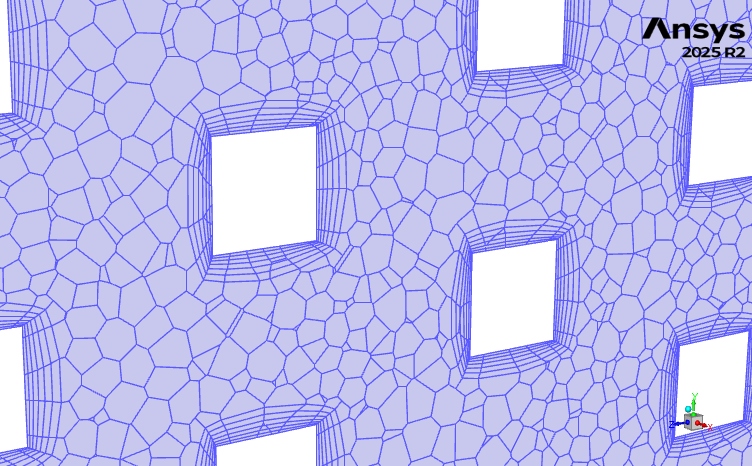
\includegraphics[
            width=\linewidth,
            trim={0 0 7cm 0},
            clip
        ]{gridmesh_A.png}
        \caption{1M cells mesh}
        \label{fig:grid_mesh_vybrana_a}
    \end{subfigure}
    \hfill
    \begin{subfigure}[t]{0.32\textwidth}
        \centering
        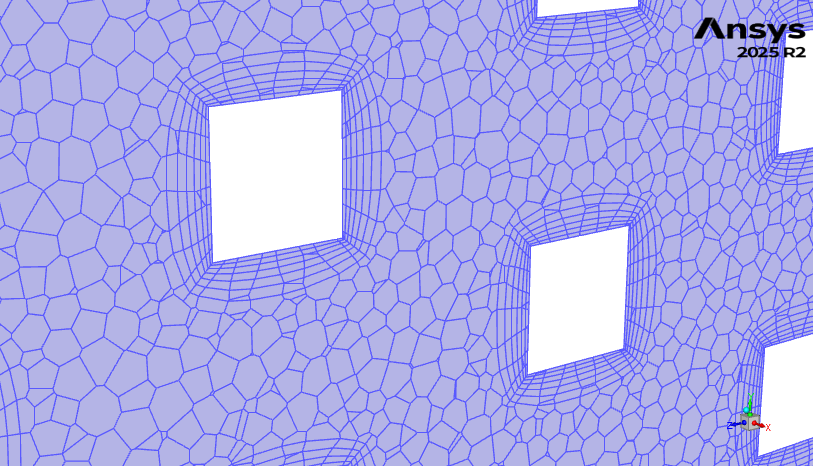
\includegraphics[
            width=\linewidth,
            trim={0 0 7cm 0},
            clip
        ]{gridmesh_C.png}
        \caption{5M cells mesh}
        \label{fig:grid_mesh_vybrana_c}
    \end{subfigure}

    \caption{A detail of the generated mesh for the CFD analysis of the porous microstructure.}
    \label{fig:grid_mesh_prehled}
\end{figure}

Figure \ref{fig:grid_mesh_vybrana_sit_a} shows the results of the mesh sensitivity analysis, where the pressure drop across the porous zone is plotted against the total number of cells in the mesh.
The mesh settings resulting in a total number of cells of 2 million provide a stable solution with minimal error in the pressure drop values, indicating that the mesh is sufficiently refined for accurate simulation results.
This mesh refinement level was selected for the subsequent CFD analysis.

\begin{figure}[h]
  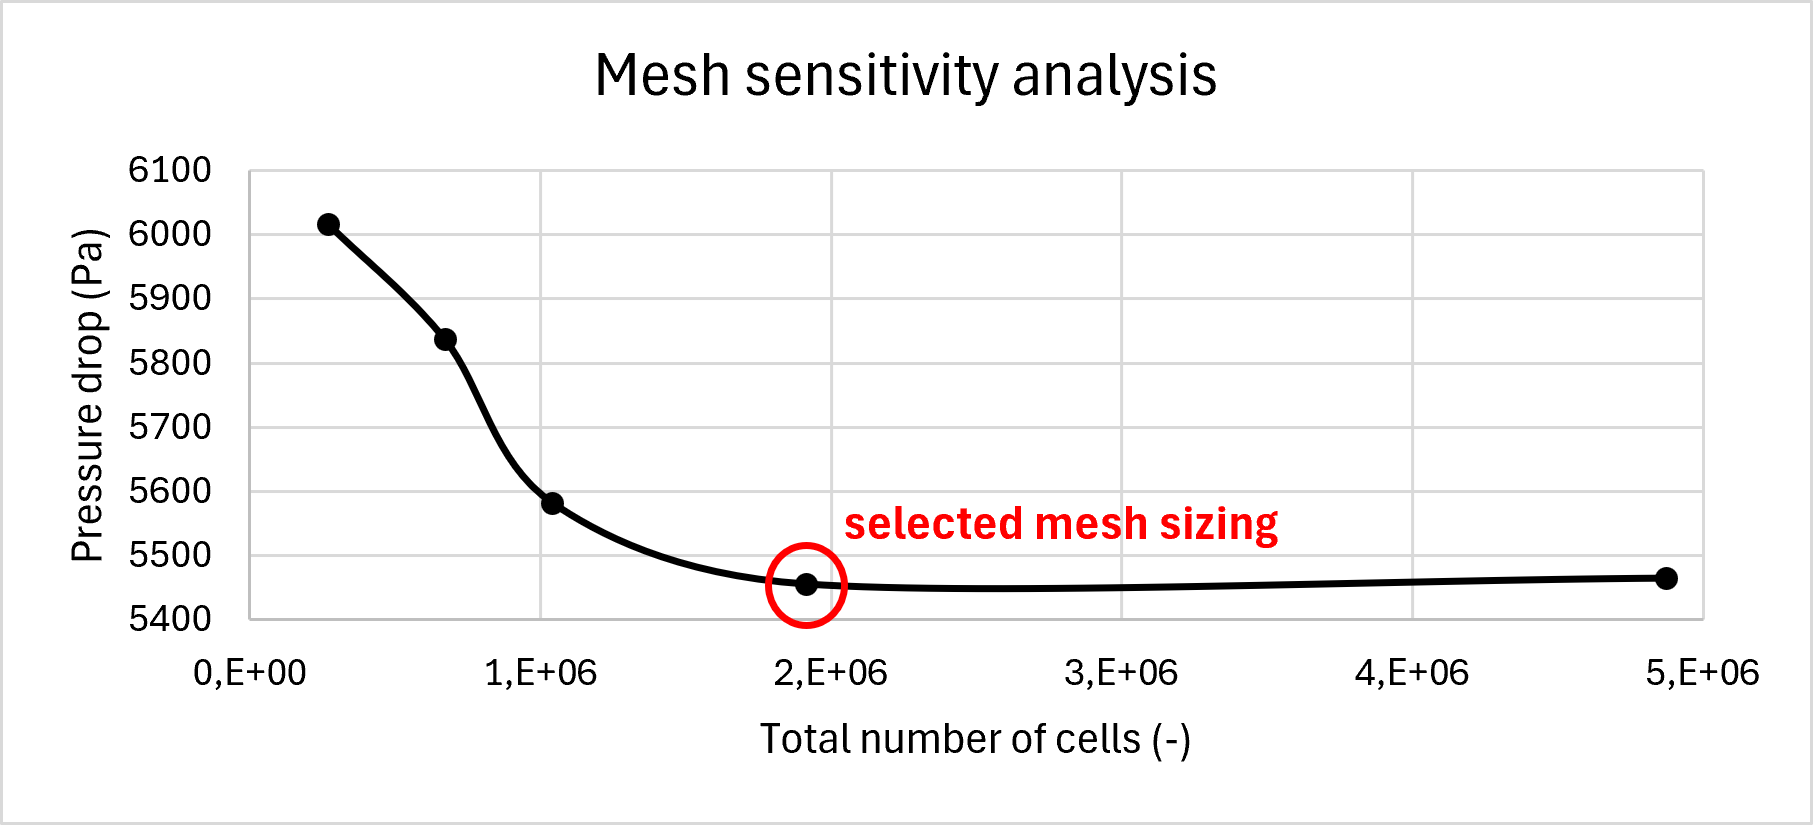
\includegraphics[width=13cm]{graf_sa_grid.png}
  \centering
  \caption{Mesh sensitivity analysis results.}
  \label{fig:grid_mesh_vybrana_sit_a}
\end{figure}

\pagebreak
\subsection{The selected mesh for the CFD analysis}
Figures \ref{fig:grid_mesh_vybrana_a22} and \ref{fig:grid_mesh_vybrana_a33} show the selected mesh for the CFD analysis.
The selected mesh settings results in mesh size of 2M cells (considering variant De).
Both shown figures provide a detailed view of the mesh structure, highlighting the refinement of the inflation layers around the walls of the porous zone and the uniformity of the mesh throughout the flow domain.
The mesh consist of polyhedra type cells and prismatic cells in the inflation layers on walls.

\begin{figure}[h]
  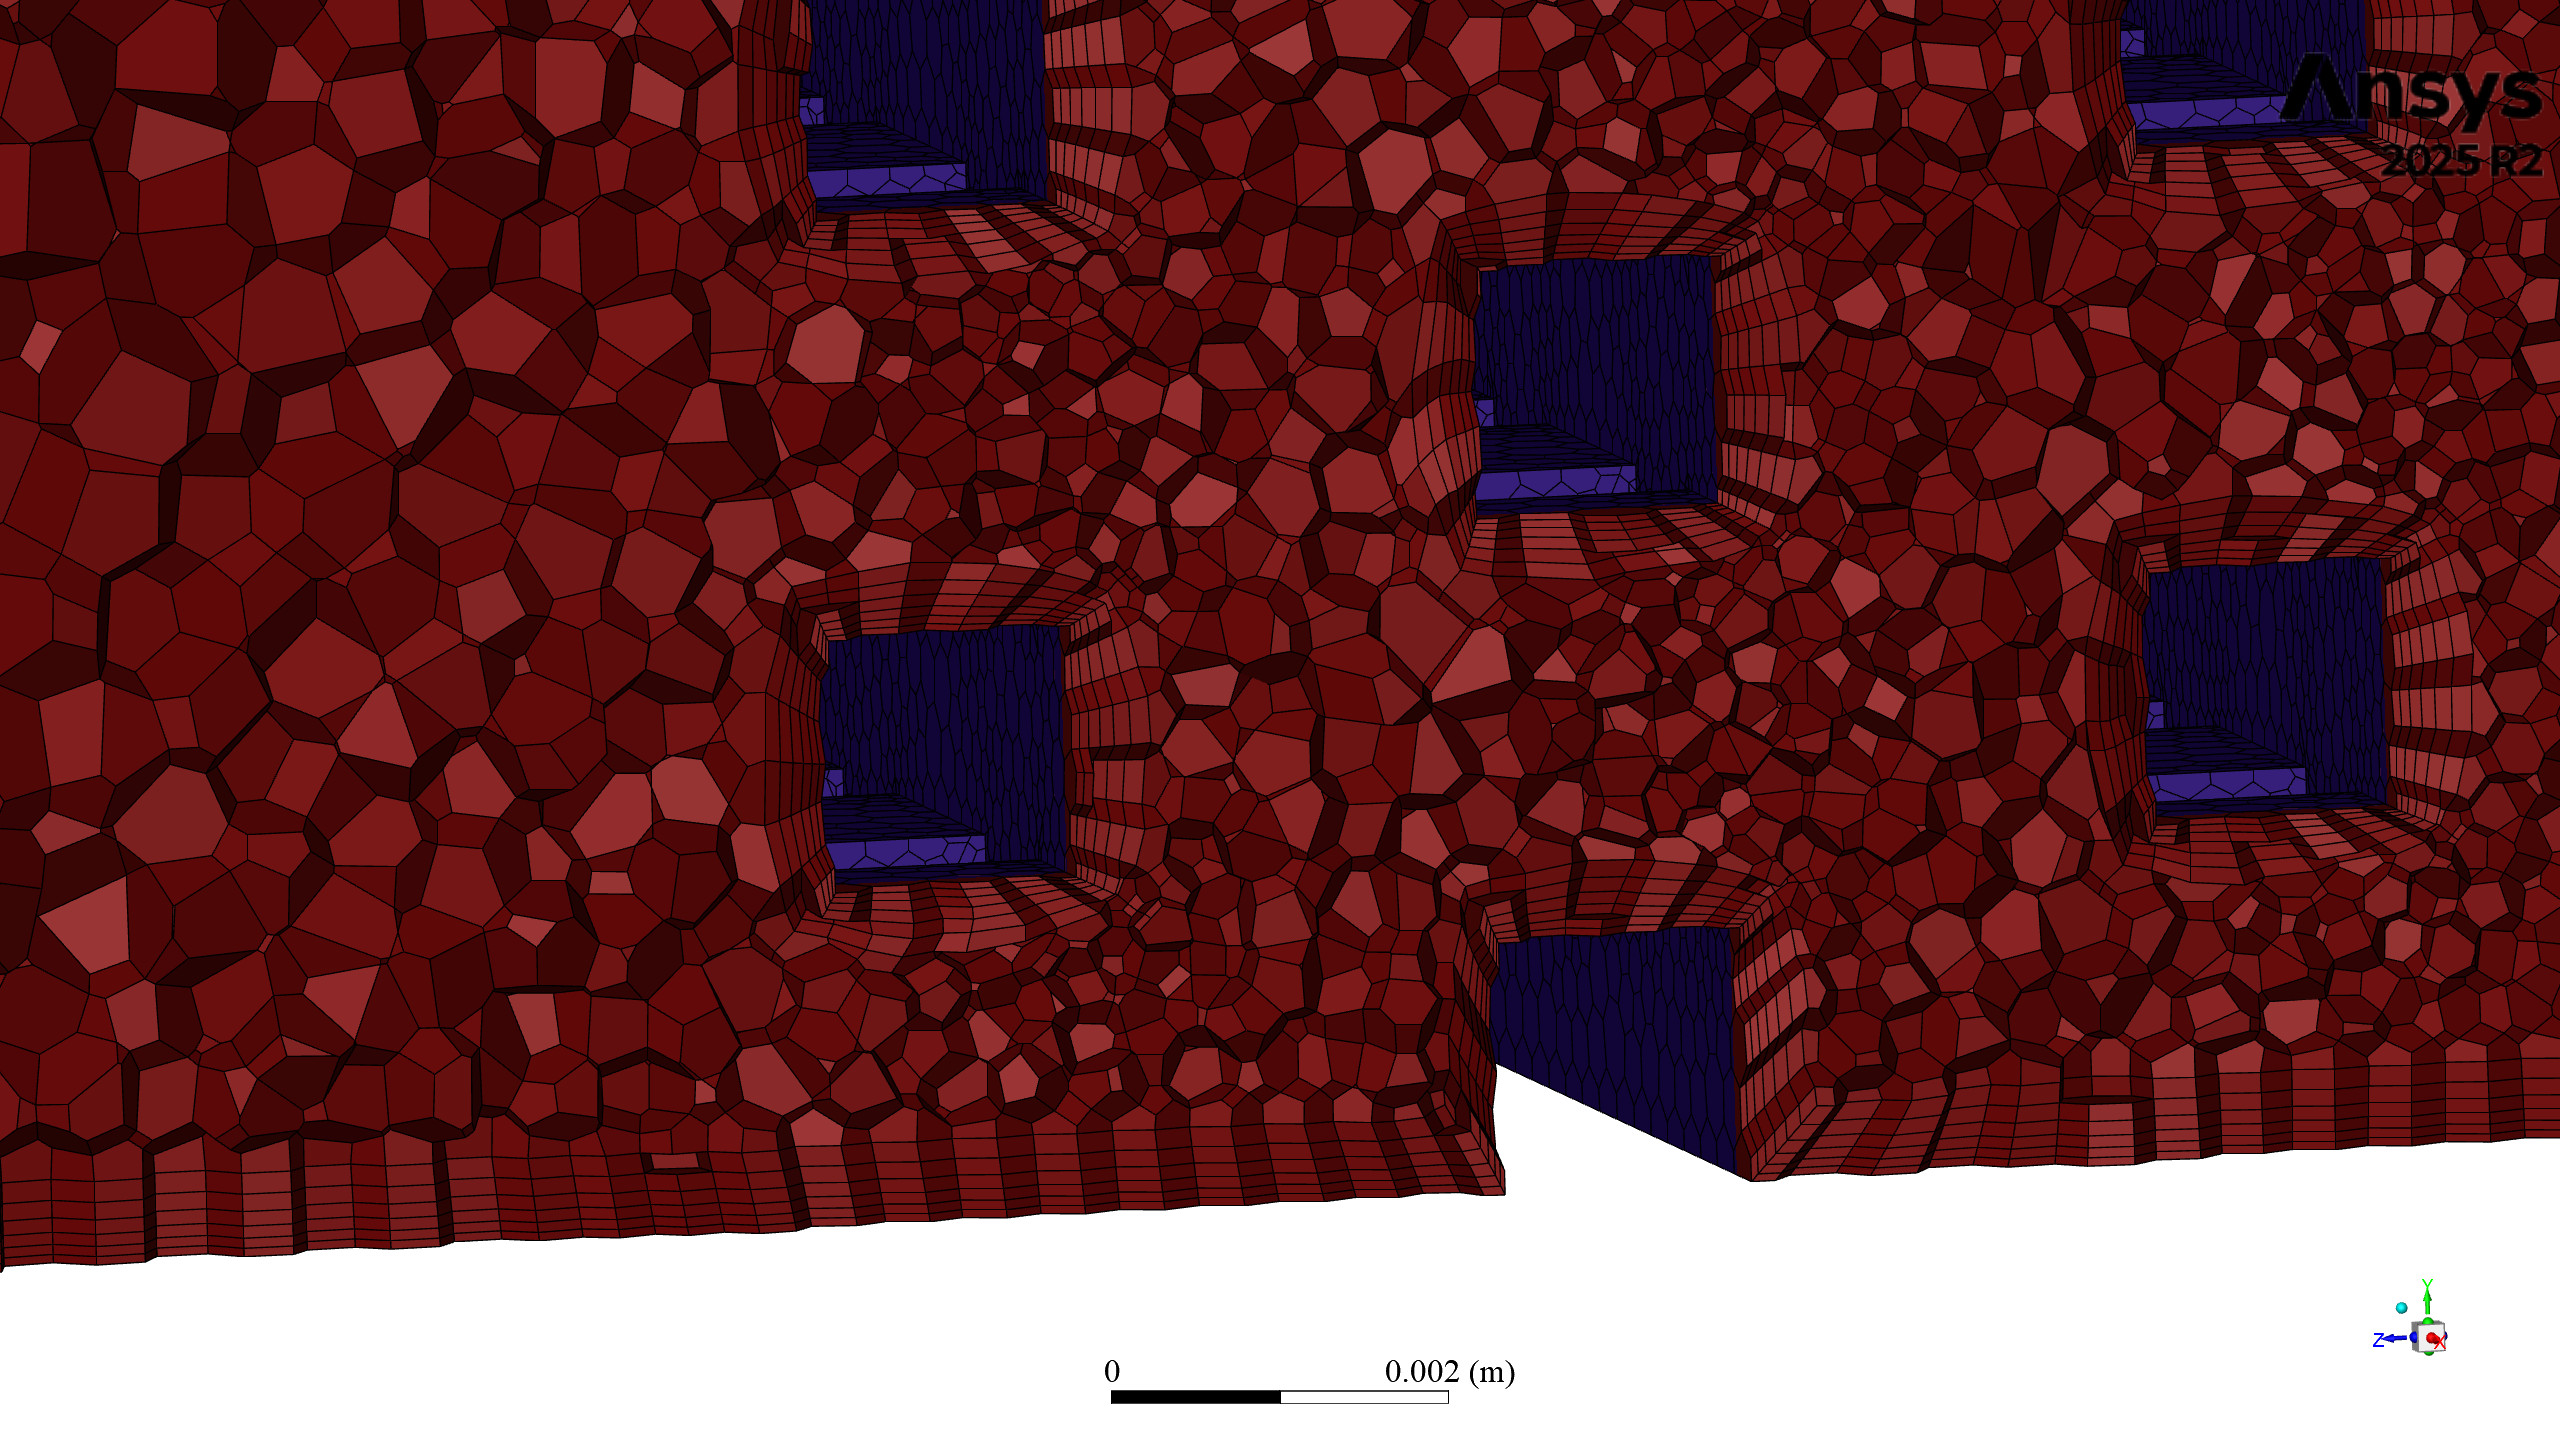
\includegraphics[width=13cm]{grid_mesh_vybrana_a.png}
  \centering
  \caption{A cross section of the selected mesh for the CFD analysis.}
  \label{fig:grid_mesh_vybrana_a22}
\end{figure}

\begin{figure}[h]
  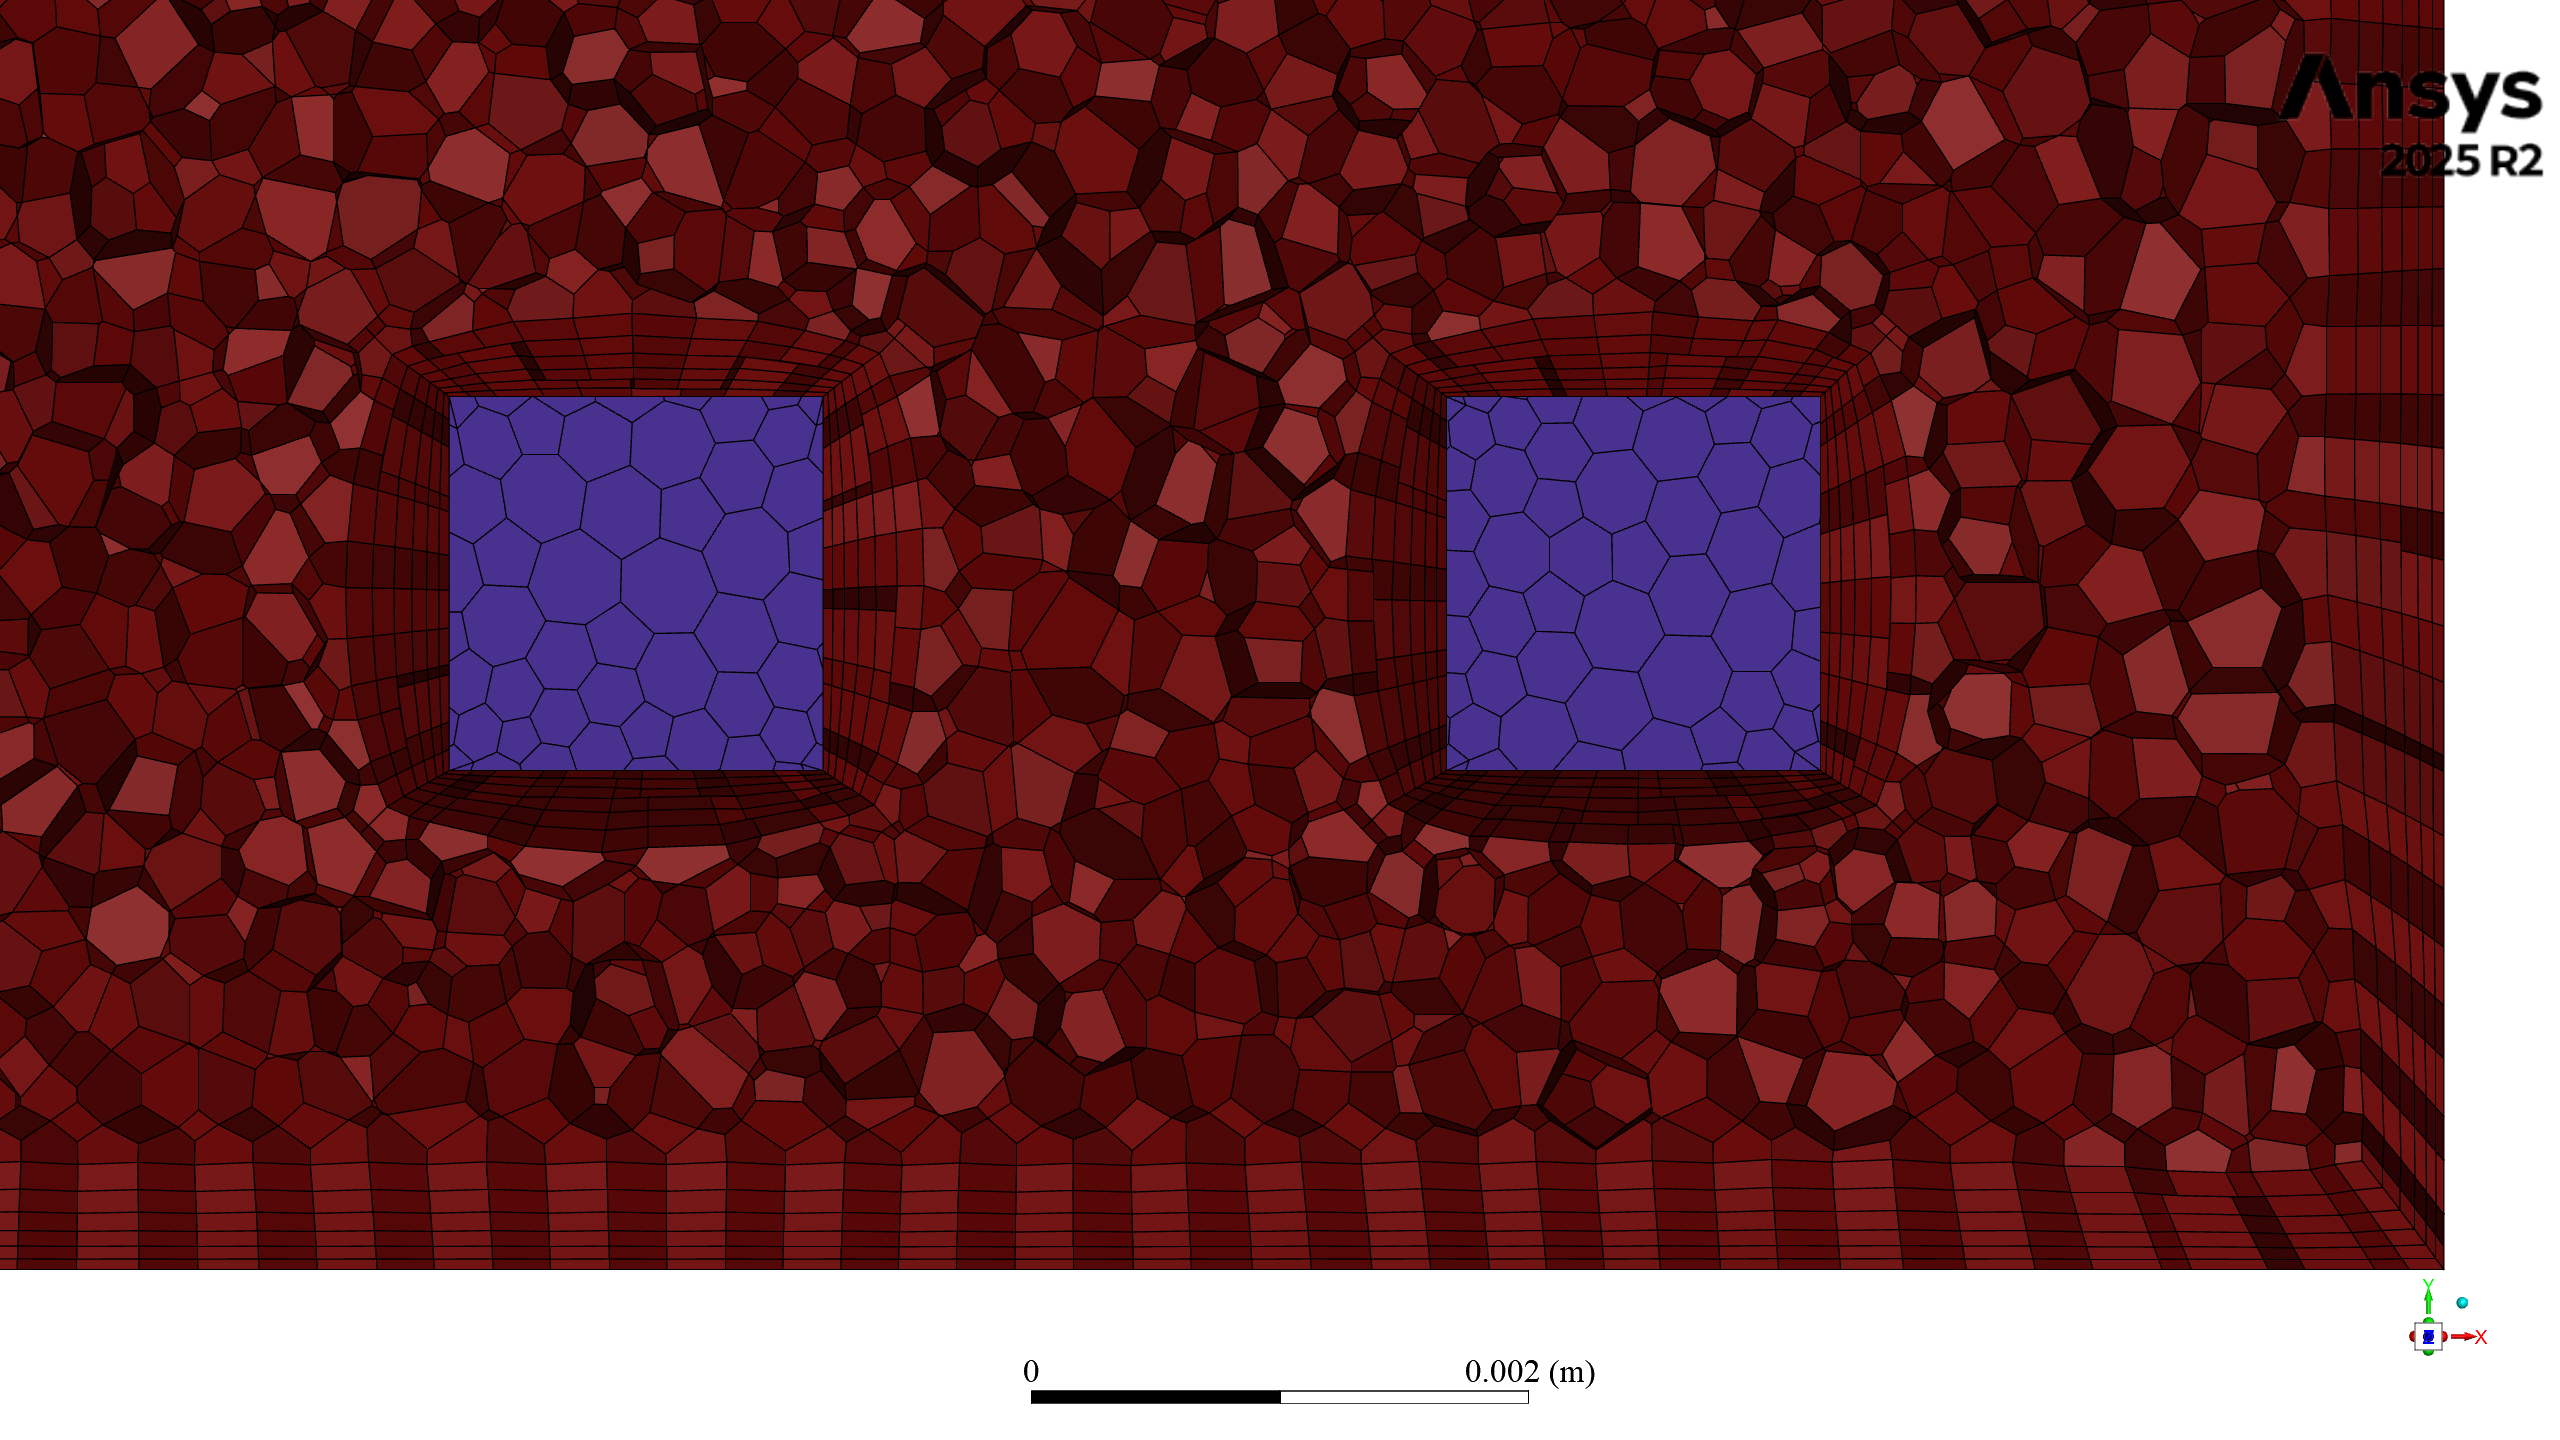
\includegraphics[width=13cm]{grid_mesh_vybrana_b.png}
  \centering
  \caption{View along the flow direction of the selected mesh.}
  \label{fig:grid_mesh_vybrana_a33}
\end{figure}


\pagebreak
\subsection{Solution}
During the solution process, the convergence of the residuals was monitored to ensure that the numerical solution reached a stable state.
The porous samples were simulated under various inlet velocity conditions, because both the linear and quadratic terms in the momentum equation are being examined in this study.
Since the parametric study consist of 35 different geometry cases, all solved on variable inlet velocity, the convergence of the residuals was evaluated for each case to ensure that the solution was accurate and reliable.
\begin{figure}[h]
  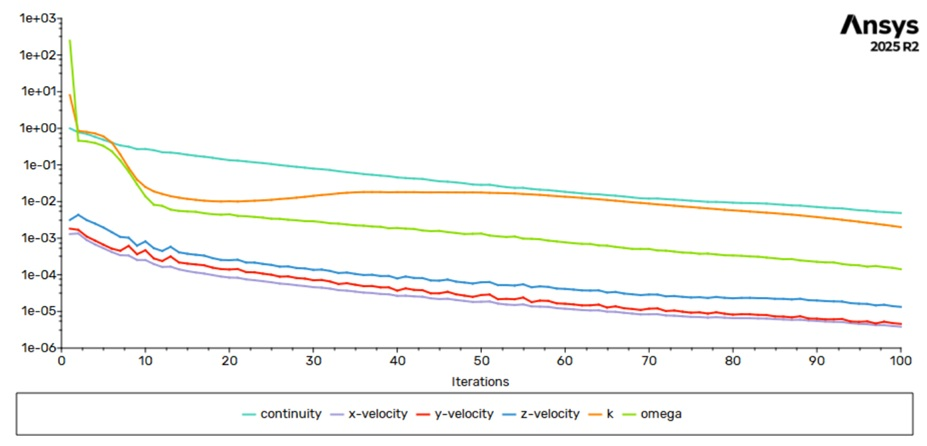
\includegraphics[width=13cm]{rezidua_grid.jpg}
  \centering
  \caption{Residuals during the solution process.}
  \label{fig:grid_mesh_vybrana_a44}
\end{figure}

To evaluate the minimal number of iterations required for convergence, the pressure drop across the porous zone was monitored during the solution process.
Figure \ref{fig:grid_mesh_vybrana_a55} shows the convergence of the pressure drop for 3 different mesh sizes, where the pressure drop stabilizes after approximately 100 iterations, indicating that the solution has reached a steady state.
Based on this analysis, 100 iterations were selected for solution of all geometry cases.

\begin{figure}[h]
  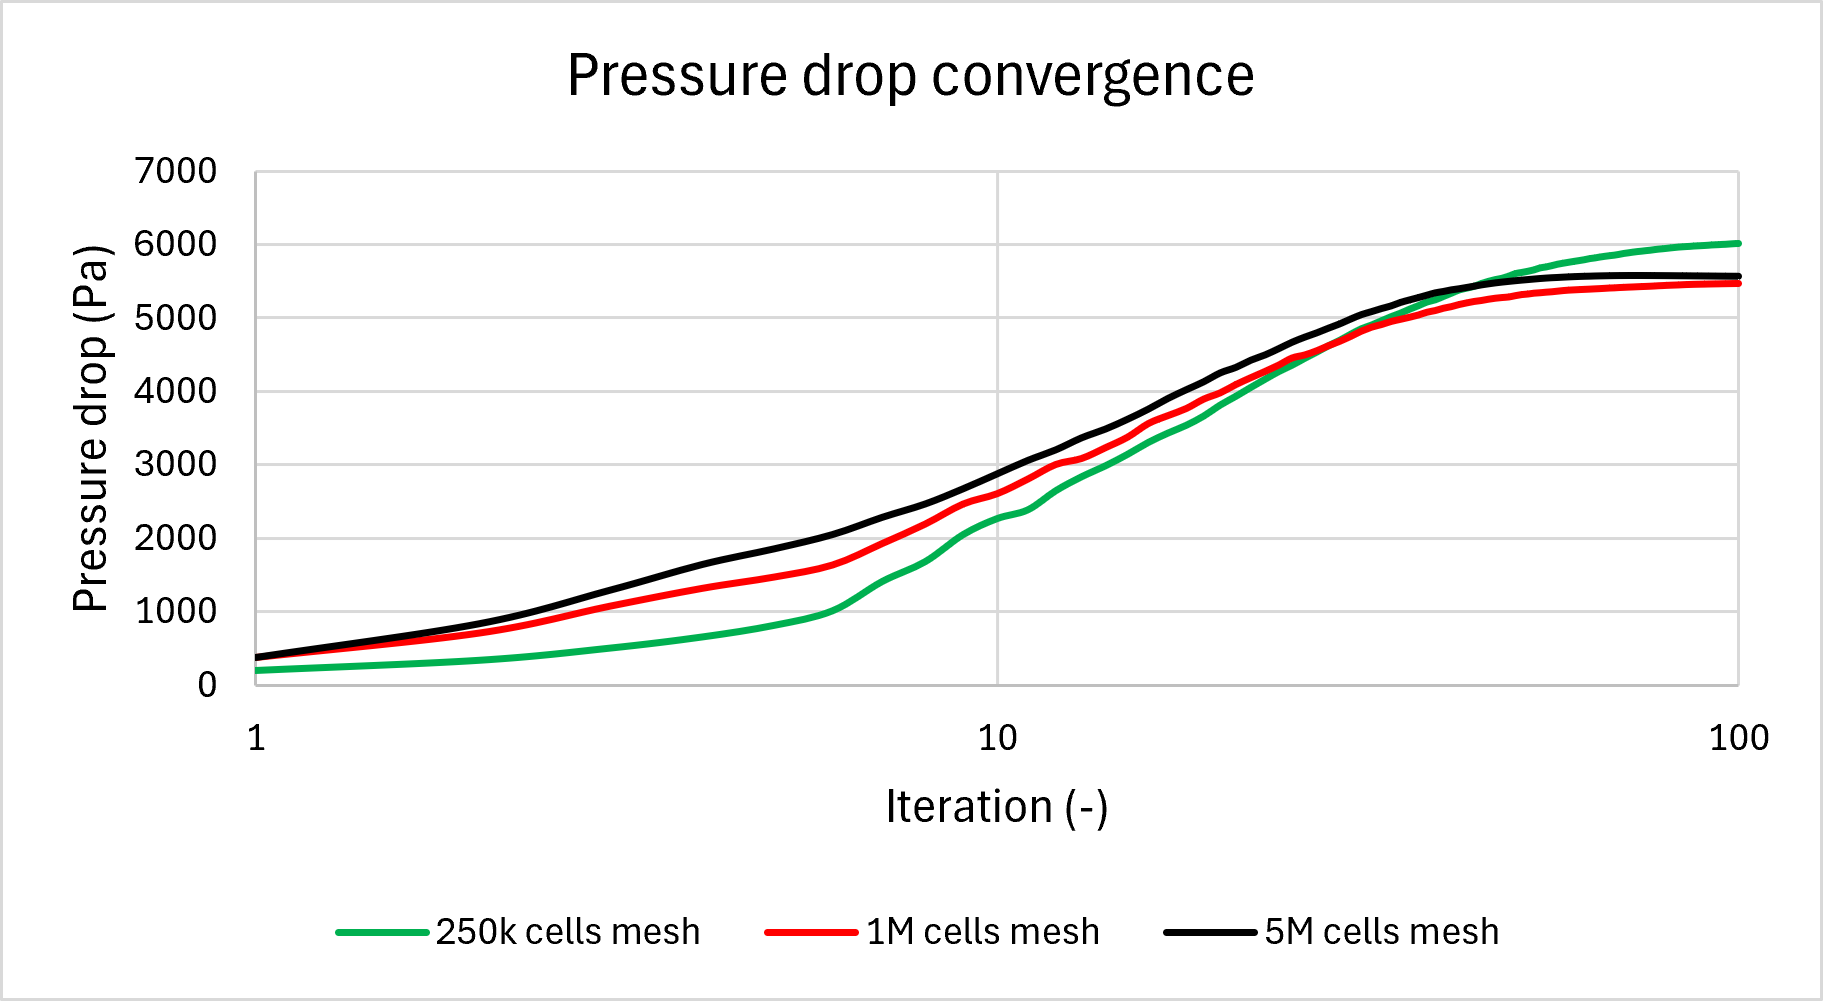
\includegraphics[width=13cm]{convergence_grid_dp.png}
  \centering
  \caption{Convergence of the pressure drop during the solution process.}
  \label{fig:grid_mesh_vybrana_a55}
\end{figure}

\pagebreak
\subsection{Results}
Figure \ref{fig:grid_mesh_vybrana_a66} shows the pressure distribution in the porous zone for the De variant.
Major part of the pressure drop occurs in the porous zone, where the flow is obstructed by the solid struts of the microstructure.
\begin{figure}[h]
  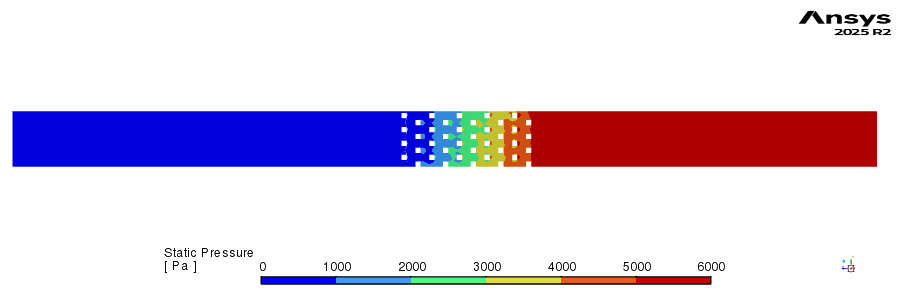
\includegraphics[width=13cm]{grid_pres_pole.png}
  \centering
  \caption{Pressure distribution in the porous zone for the De variant.}
  \label{fig:grid_mesh_vybrana_a66}
\end{figure}
Figure \ref{fig:grid_mesh_vybrana_a77} shows the velocity distribution in the porous zone for the De variant.
Flow patterns are complex, but periodic, with regions of high velocity in the narrow channels between the solid struts.

\begin{figure}[h]
  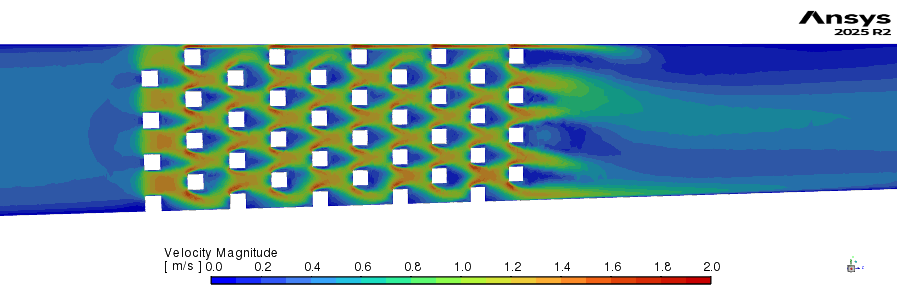
\includegraphics[width=13cm]{grid_vel_pole.png}
  \centering
  \caption{Velocity distribution in the porous zone for the De variant.}
  \label{fig:grid_mesh_vybrana_a77}
\end{figure}

\begin{figure}[h]
  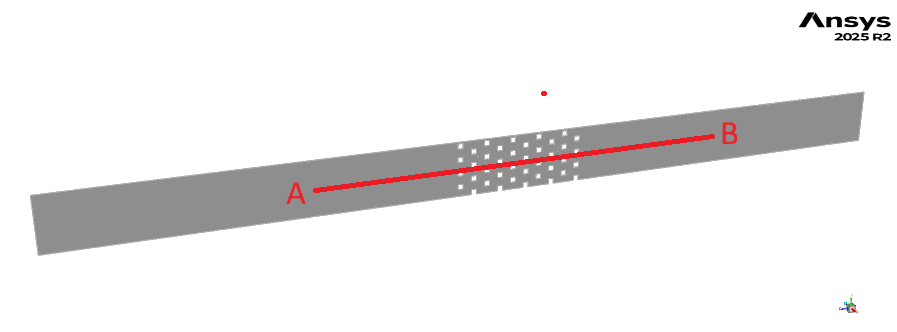
\includegraphics[width=13cm]{grid_line.png}
  \centering
  \caption{A line created to evaluate the velocity and pressure distribution along the flow direction.}
  \label{fig:grid_mesh_vybrana_a88}
\end{figure}
Figure \ref{fig:grid_mesh_vybrana_a88} shows a line created to evaluate the velocity and pressure distribution along the flow direction in the porous zone for the De variant.
The resulting pressure drop and velocity profile along the flow direction in the porous zone for the De variant are shown in Figures \ref{fig:grid_mesh_vybrana_a99} and \ref{fig:grid_mesh_vybrana_a100}, respectively.
The goal of this result evaluation is to examine if the geometry region is CFD model is large enough to provide a fully developed flow in the porous zone.
Both the pressure drop and velocity profile show a periodic behavior, indicating that the flow is fully developed in the porous zone and that the geometry region is sufficient for accurate simulation results.

\begin{figure}[h]
  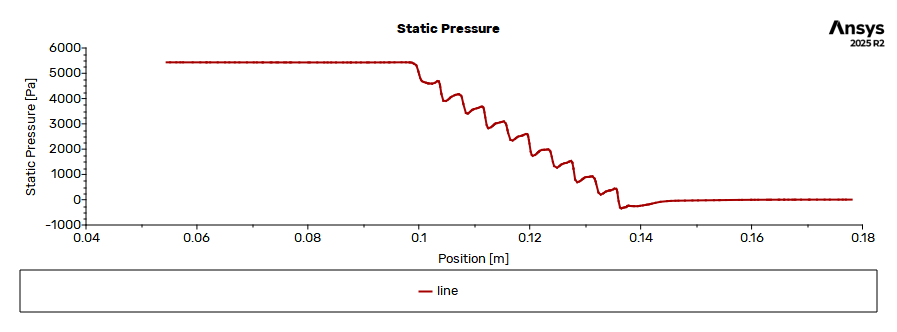
\includegraphics[width=13cm]{grid_press.png}
  \centering
  \caption{Pressure drop along the flow direction in the porous zone for the De variant.}
  \label{fig:grid_mesh_vybrana_a99}
\end{figure}

\begin{figure}[h]
  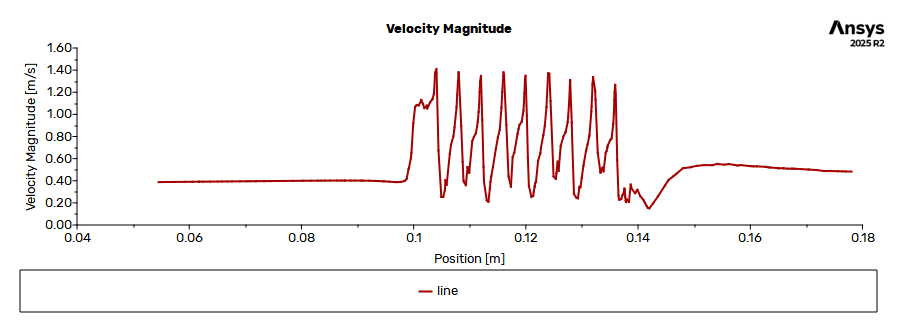
\includegraphics[width=13cm]{grid_vel.png}
  \centering
  \caption{Velocity profile along the flow direction in the porous zone for the De variant.}
  \label{fig:grid_mesh_vybrana_a100}
\end{figure}

The pressure profile shown in Figure~\ref{fig:grid_mesh_vybrana_a99} demonstrates that the pressure decreases almost exclusively within the porous region, whereas the inlet and outlet sections exhibit only negligible pressure gradients. This behaviour confirms that the selected channel length is sufficient to eliminate the influence of the boundary conditions on the evaluated pressure loss. Similarly, the velocity profile presented in Figure~\ref{fig:grid_mesh_vybrana_a100} exhibits periodic oscillations corresponding to the repeated unit-cell geometry of the porous structure. The alternating acceleration and deceleration of the flow results from the continuous contraction and expansion of the flow passages between neighbouring solid ligaments. Since the amplitude and periodicity of these oscillations remain nearly constant throughout the porous region, the flow can be considered fully developed. Consequently, the chosen computational domain is sufficiently large to accurately represent the hydraulic behaviour of the periodic porous structure while avoiding unnecessary computational cost associated with a larger numerical model.

\newpage
\subsection{Validation of the numerical model}
The numerical model was validated by comparing the CFD simulation results with experimental data obtained from the TEALC experimental loop.
The selected geometry cases for validation were Ba and Da, which represent two different porous structures.
Figures \ref{fig:grid_mesh_vybrana_a1002} shows the 3D-printed samples used for the experimental validation, which were manufactured using a high-resolution 3d printer to accurately replicate the porous microstructure.
Samples dimensions are 40x40x15 mm.

\begin{figure}[h]
  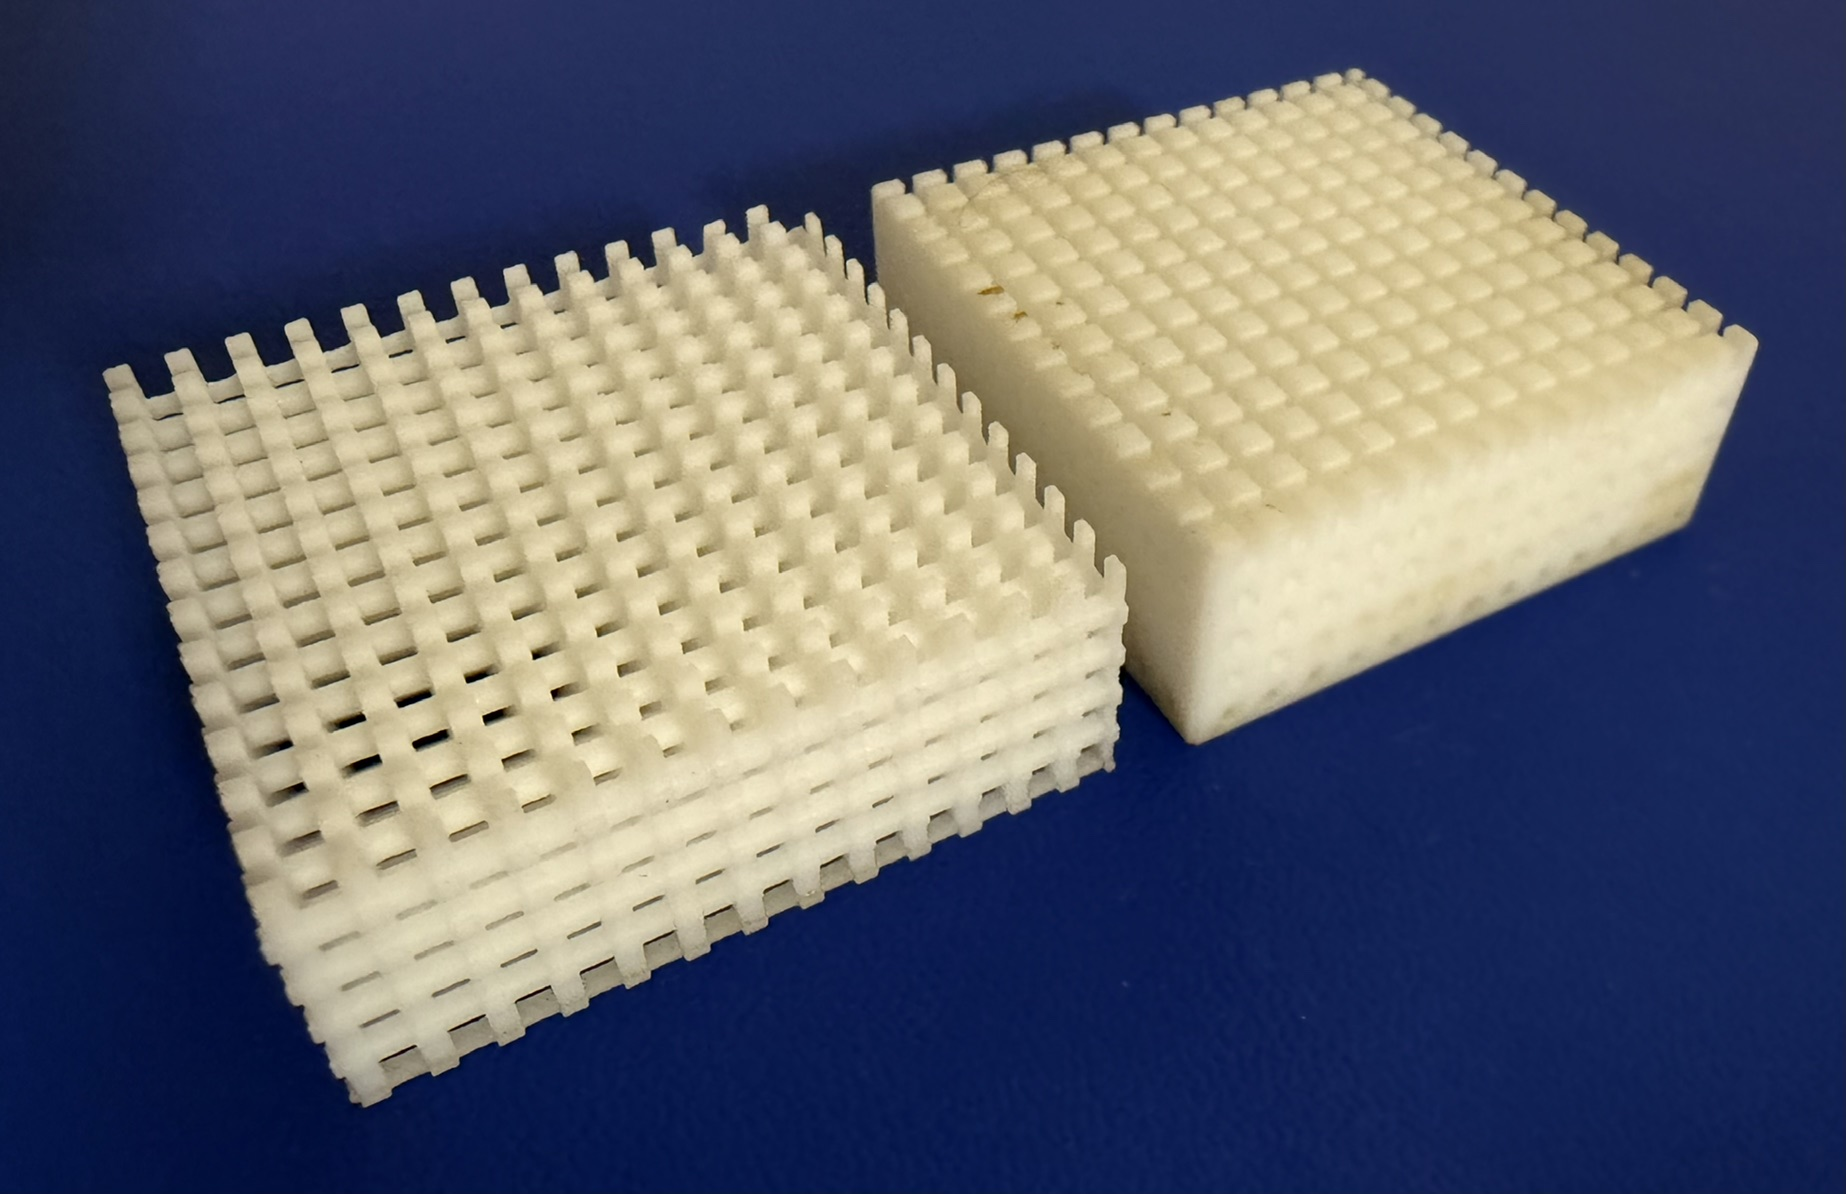
\includegraphics[width=7.5cm]{foto_vzorku_k_validaci.jpeg}
  \centering
  \caption{3D-printed samples Ba (left) and Da (right).}
  \label{fig:grid_mesh_vybrana_a1002}
\end{figure}

Figure \ref{fig:grid_mesh_vybrana_a1001} shows the comparison of the pressure drop across the porous zone for both geometry cases, where the CFD results are in good agreement with the experimental data, indicating that the numerical model is capable of accurately predicting the pressure drop in porous materials.

\begin{figure}[h]
  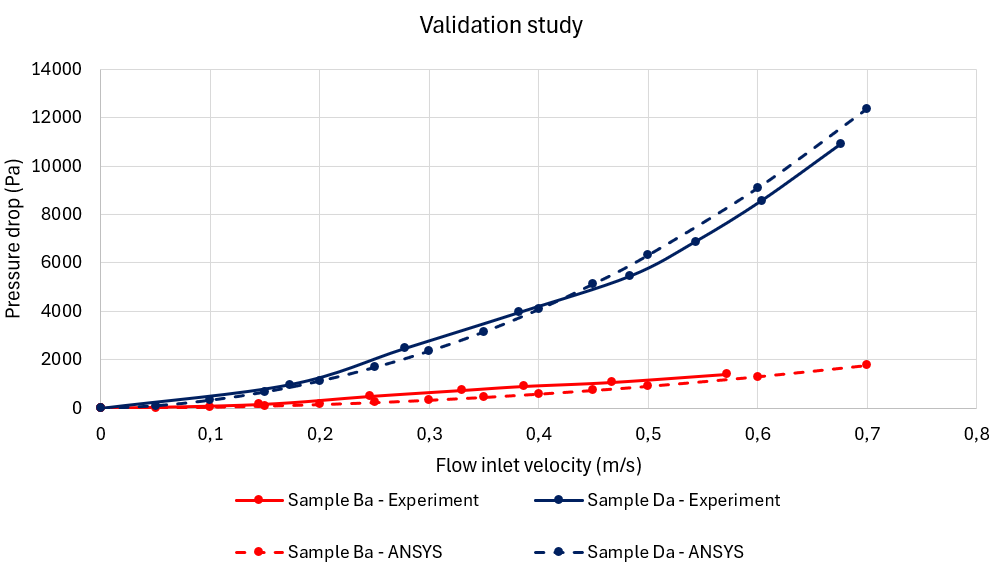
\includegraphics[width=12cm]{graf_validace_grid.png}
  \centering
  \caption{Validation of the CFD model, samples Ba and Da.}
  \label{fig:grid_mesh_vybrana_a1001}
\end{figure}

The comparison between the experimental measurements and the CFD predictions demonstrates a very good agreement over the entire investigated velocity range. For both samples, the majority of the predicted pressure drops are within approximately 10~\% of the experimental values, while the maximum deviations are generally within 10–15~\% at higher flow velocities. The CFD model successfully reproduces both the overall trend and the nonlinear increase in pressure drop with increasing inlet velocity. Considering the inherent uncertainties associated with both numerical simulations and experimental measurements, the observed agreement is considered satisfactory, and the CFD model can therefore be regarded as validated for the investigated flow conditions.

\newpage
\subsection{Parametric study results - pressure drop characteristics}
The parametric study results show the relationship between porosity, tortuosity, and pressure drop. The goal is to evaluate the influence of these parameters on the pressure drop in the porous zone and to create a predictive equation.

\begin{figure}[h]
  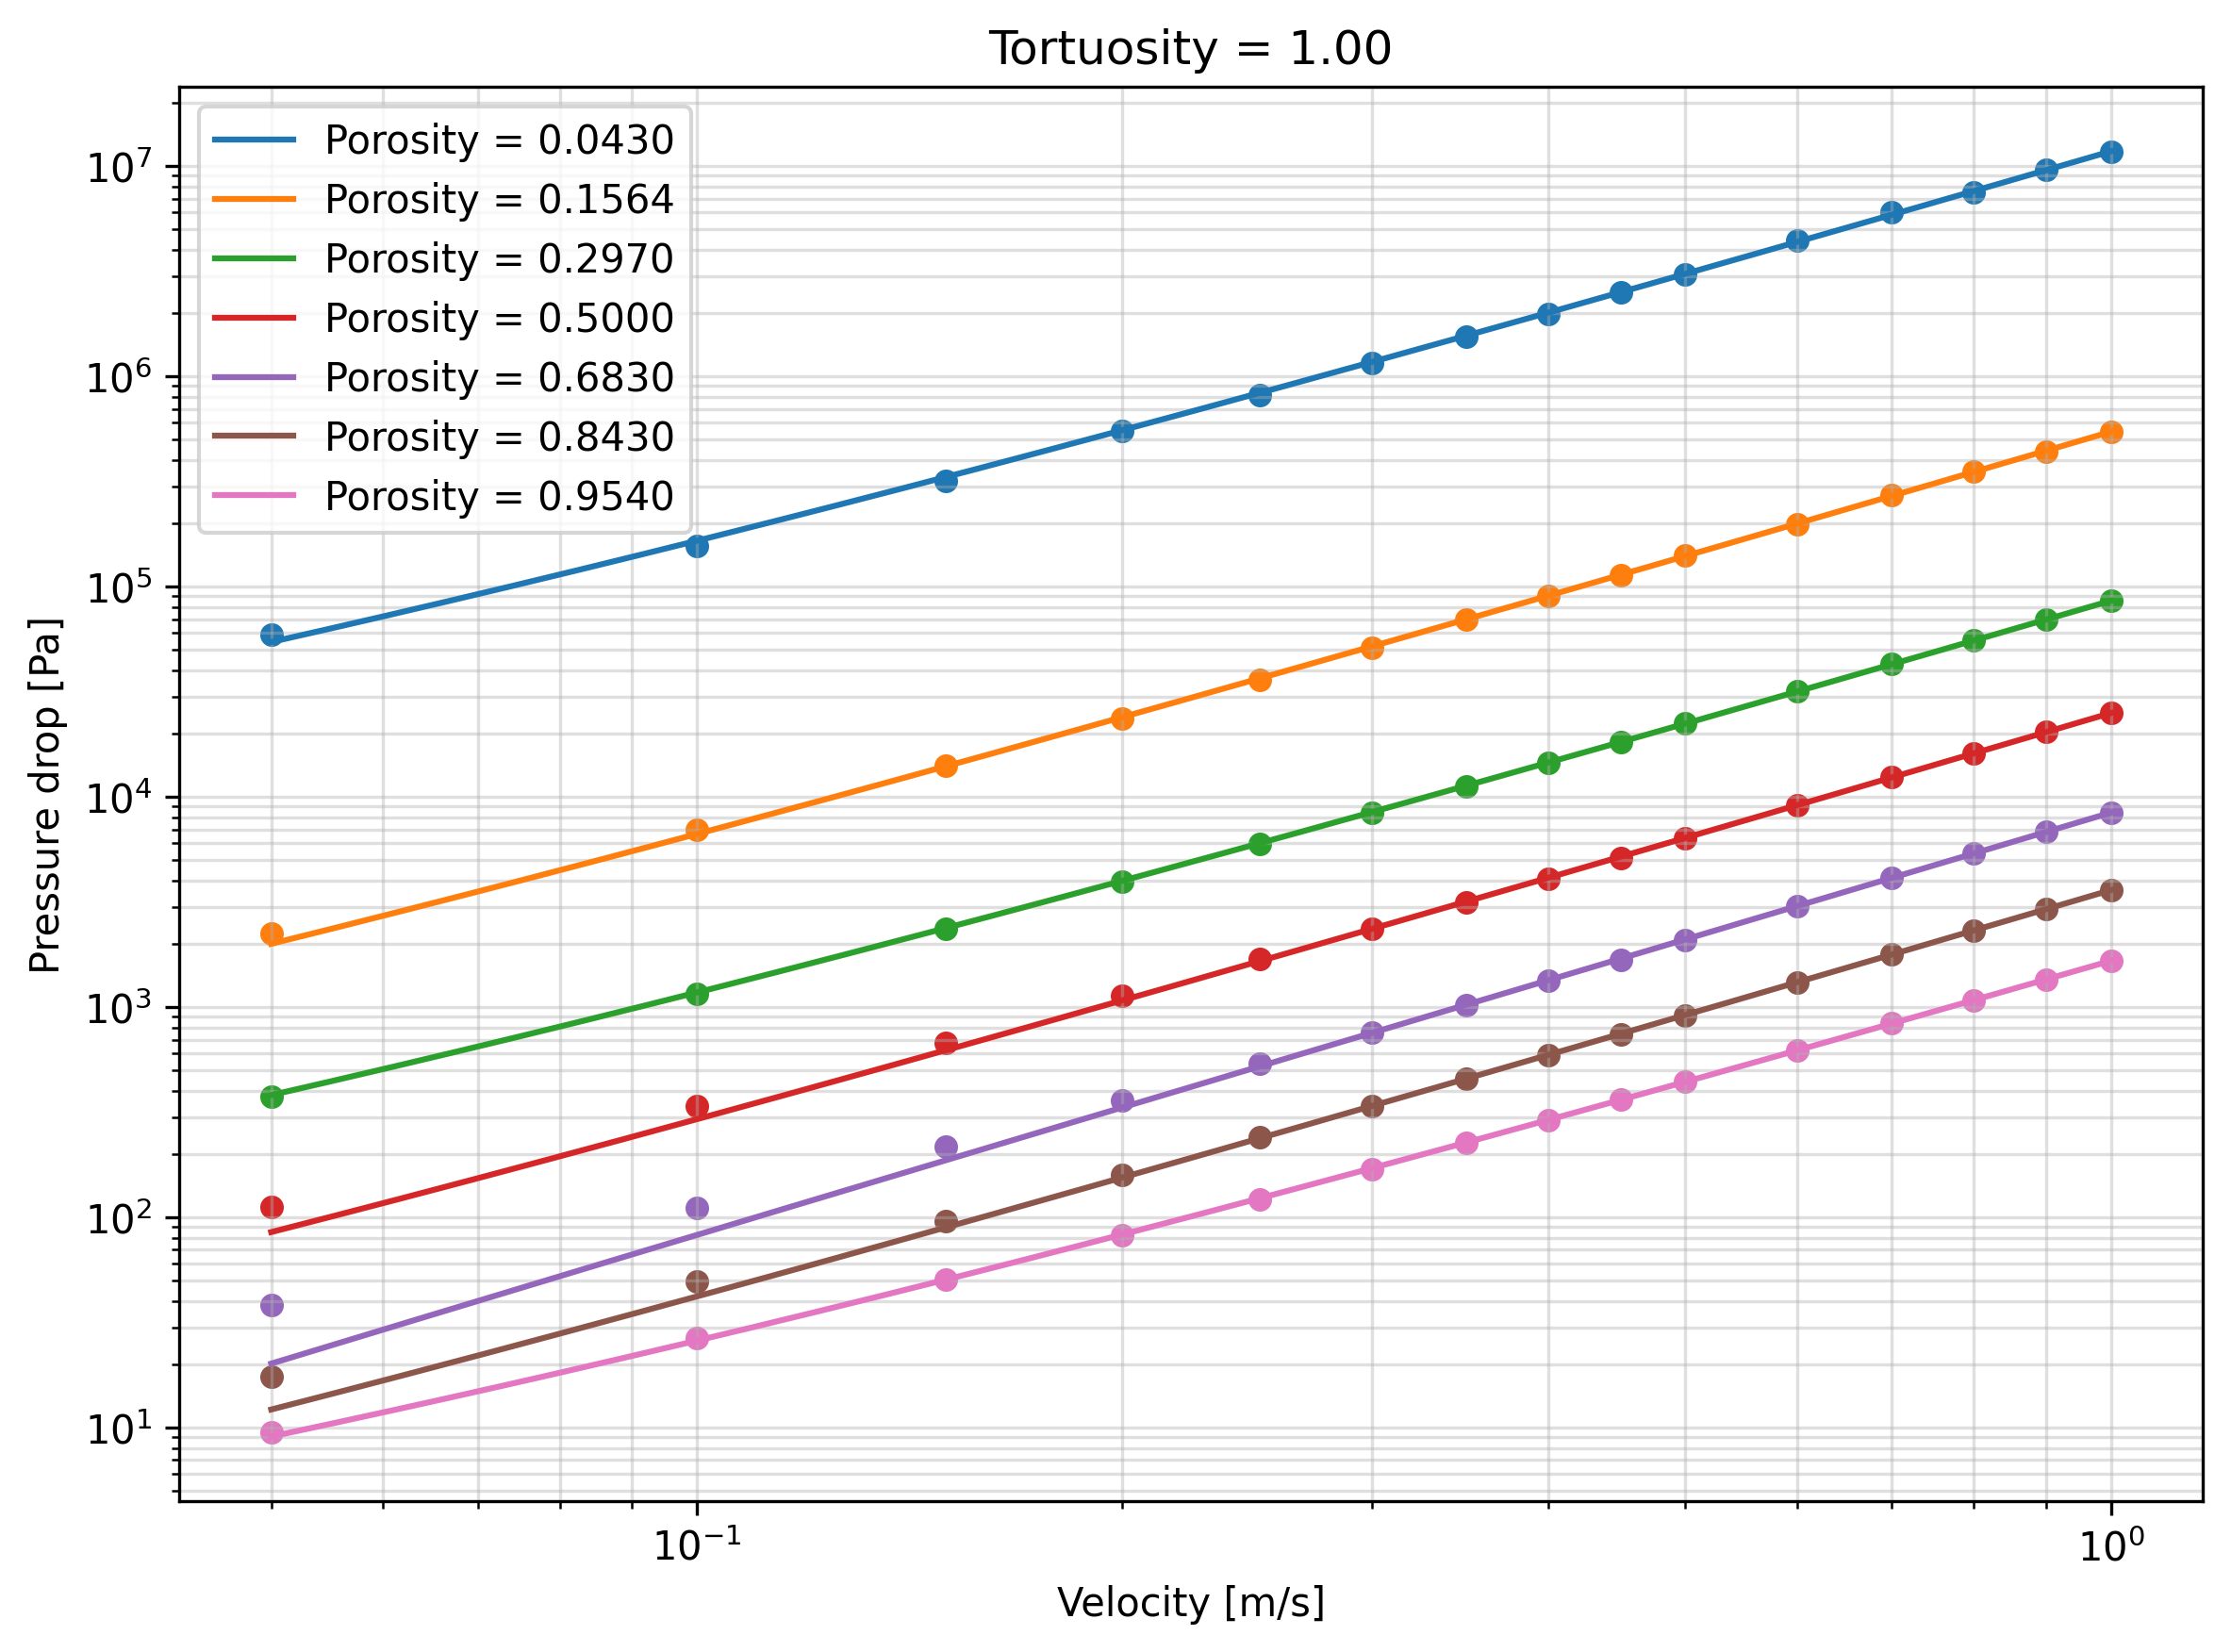
\includegraphics[width=14cm]{gr_tor1.png}
  \centering
  \caption{Resulting pressure drop characteristics, Tortuosity = 1}
  \label{fig:gr_tor1}
\end{figure}

The pressure drop data were processed separately for each combination of porosity and tortuosity. The original dataset contained the superficial velocity and the corresponding pressure drop values, while the sample identifiers and tortuosity indices were converted into their respective physical values. For each dataset, the pressure drop was approximated using the Darcy--Forchheimer equation

\begin{equation}
\Delta p = A v + B v^{2},
\end{equation}

where $\Delta p$ is the pressure drop, $v$ is the superficial velocity, and $A$ and $B$ are the fitted coefficients. The coefficients were obtained using a least-squares regression without an intercept, assuming that the pressure drop approaches zero as the flow velocity tends to zero.

The fitted coefficients were subsequently converted into the intrinsic permeability $K$ and the Forchheimer coefficient $\beta$ according to

\begin{equation}
K = \frac{\mu L}{A},
\end{equation}

and

\begin{equation}
\beta = \frac{B}{\rho L},
\end{equation}

where $\mu$ is the dynamic viscosity of the fluid, $\rho$ is the fluid density, and $L$ is the thickness of the porous sample.

For each tortuosity level, the calculated pressure drop values are shown as discrete markers, while the solid curves represent the fitted Darcy--Forchheimer model. Although the fitting procedure was performed in linear coordinates, both axes are displayed on a logarithmic scale to improve the visualization of data spanning several orders of magnitude. The results demonstrate a monotonic increase in pressure drop with increasing superficial velocity for all investigated structures. At a given velocity, the pressure drop decreases systematically with increasing porosity, reflecting the lower hydraulic resistance associated with more open porous media.

\begin{figure}[h]
  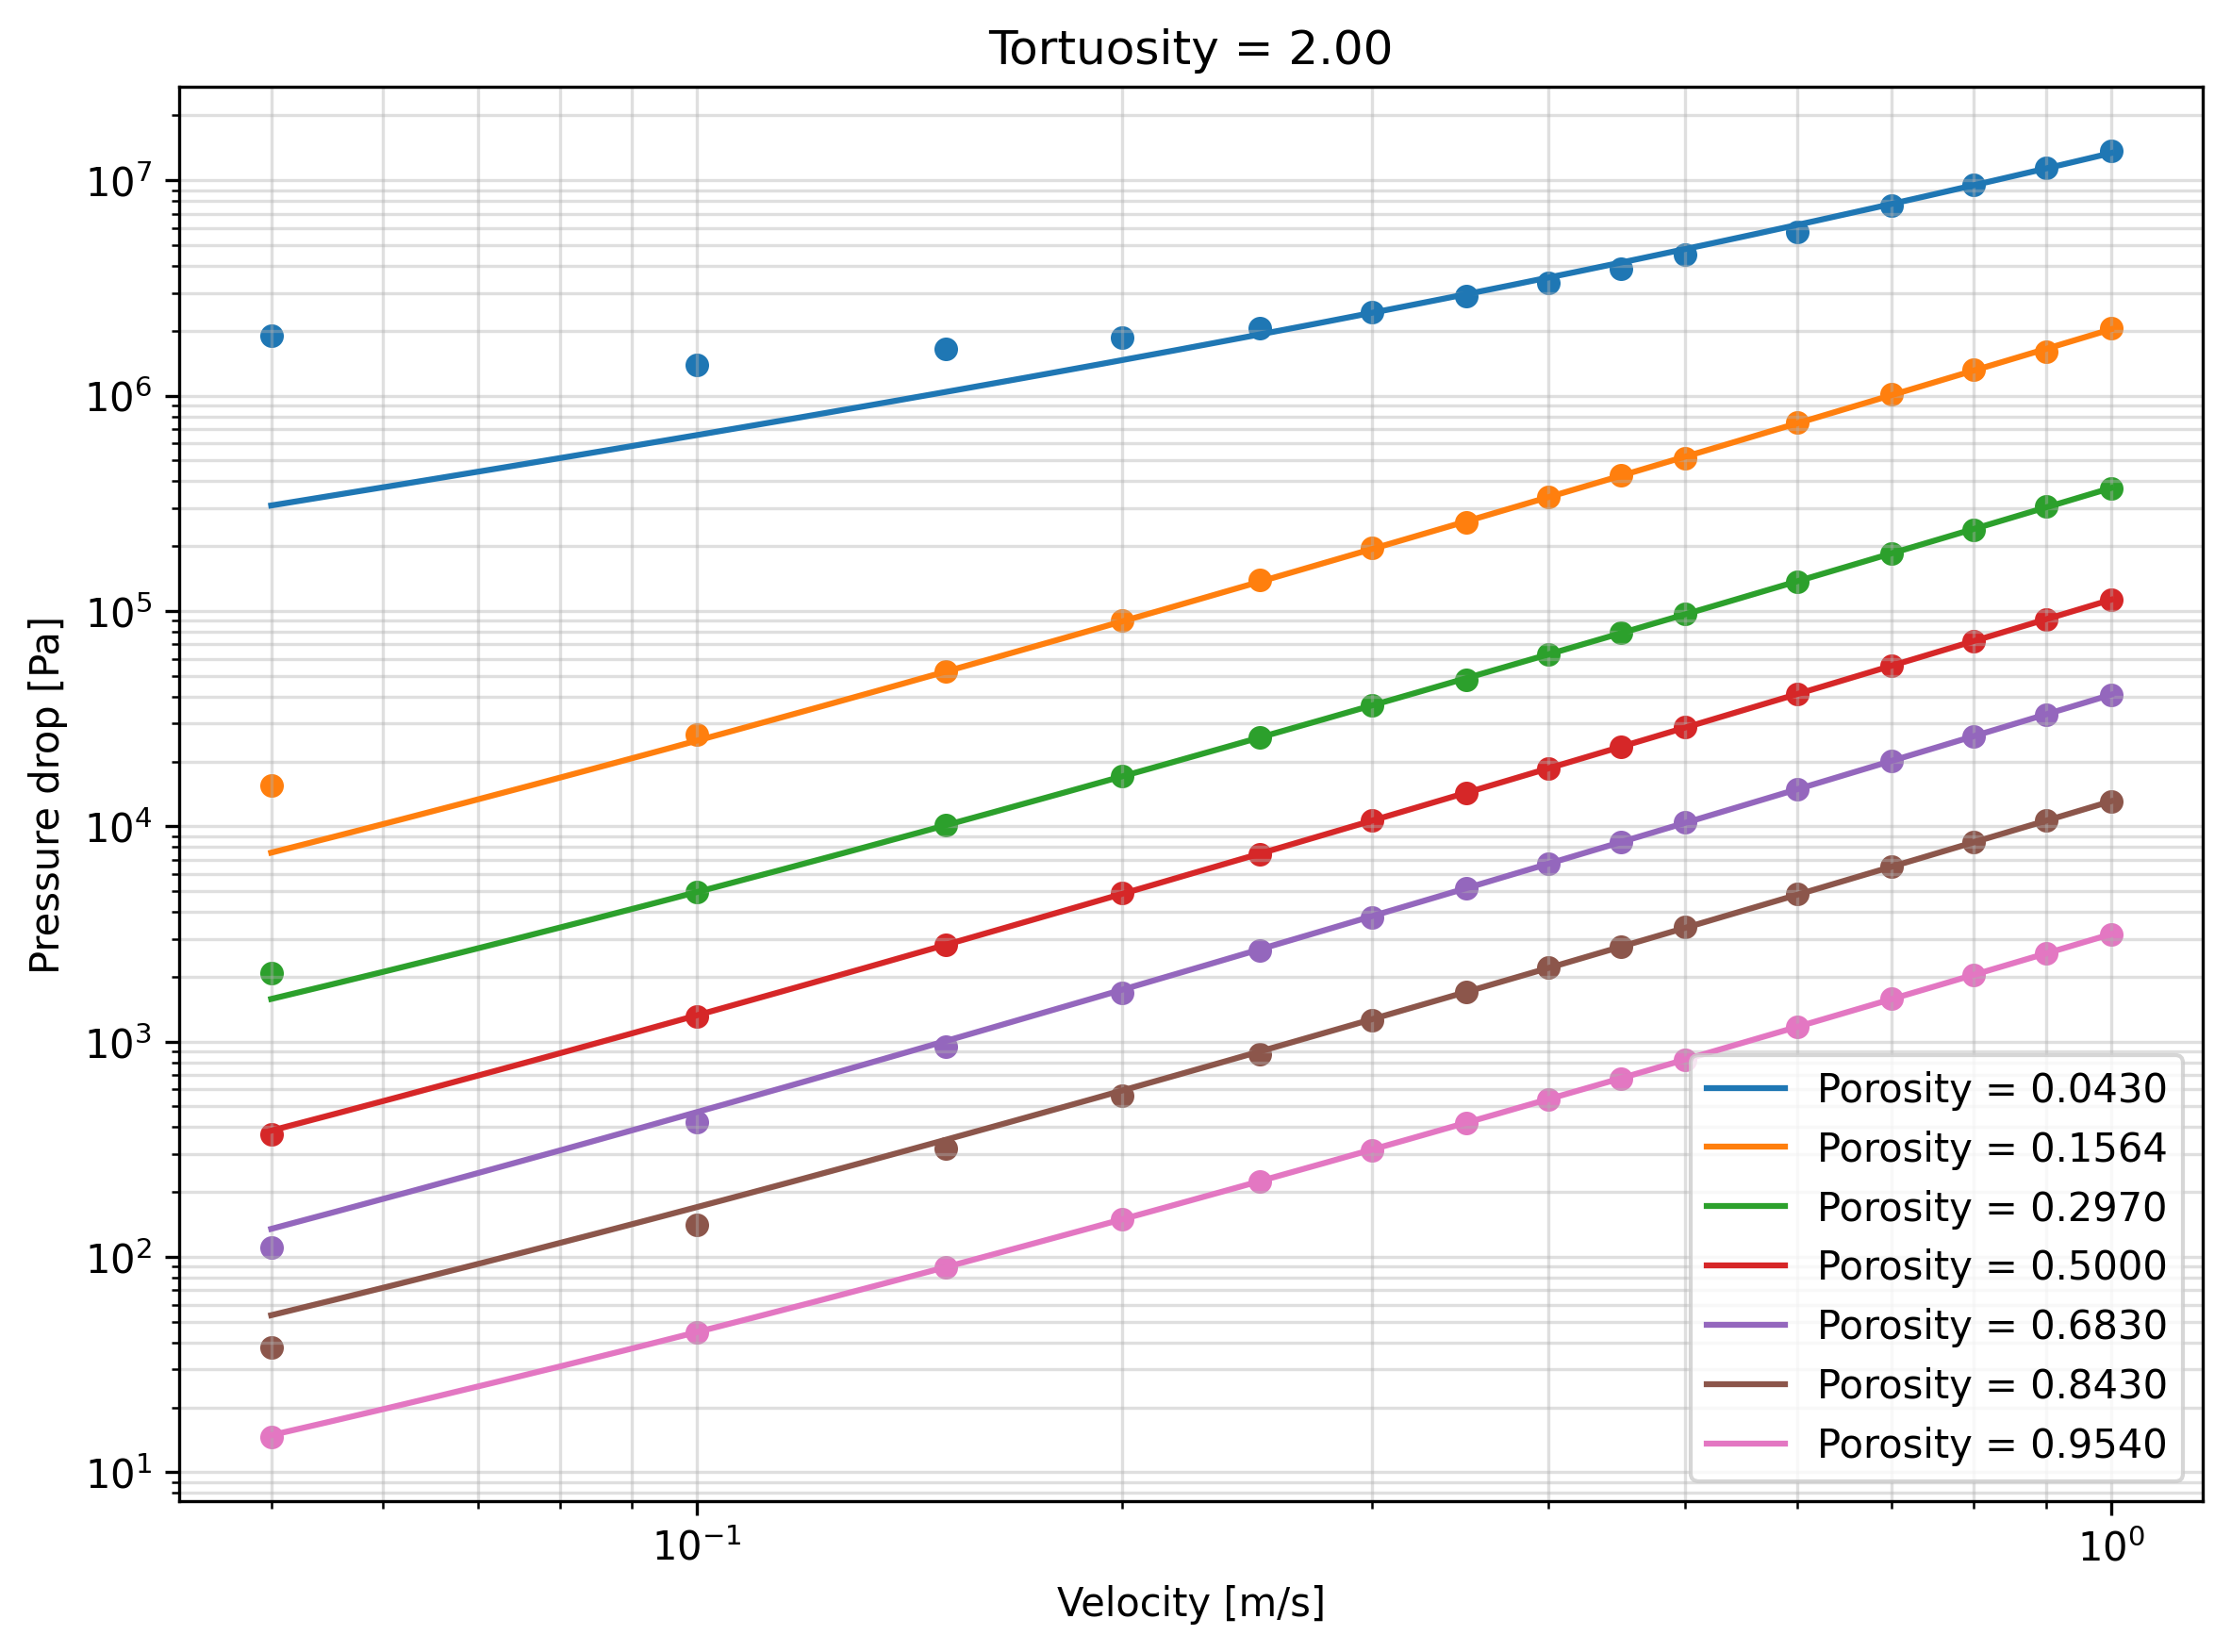
\includegraphics[width=14cm]{gr_tor2.png}
  \centering
  \caption{Resulting pressure drop characteristics, Tortuosity = 2}
  \label{fig:gr_tor2}
\end{figure}

This chapter presents the results of numerical study for Tortuosity = 1 and Tortuosity = 2, which are the two extreme cases of the investigated range. The intermediate tortuosity levels exhibit similar trends, with the pressure drop characteristics falling between the two presented cases. A complete overview of the pressure drop characteristics for all investigated tortuosity levels is provided in Appendix A.
\pagebreak

\subsection{Parametric study results -- permeability and Forchheimer coefficient}
\label{sec:parametric_study_results}

The parametric study was performed to determine how the hydraulic behaviour of
the investigated porous structures is affected by their microstructural
properties. For each generated geometry, the pressure-loss data were evaluated
using the Darcy--Forchheimer equation,

\begin{equation}
\frac{\Delta p}{L}
=
\frac{\mu}{K}u
+
\rho\beta u^{2},
\label{eq:darcy_forchheimer_parametric}
\end{equation}

where $\Delta p$ is the pressure loss, $L$ is the length of the porous region,
$\mu$ is the dynamic viscosity, $K$ is the permeability, $u$ is the superficial
velocity, $\rho$ is the fluid density and $\beta$ is the Forchheimer
coefficient.

Permeability describes the viscous resistance of the porous medium, whereas
the Forchheimer coefficient characterises the additional nonlinear pressure
losses associated with inertial effects. Both quantities were subsequently
related to two microstructural parameters obtained from the geometrical
analysis: porosity $\varepsilon$ and tortuosity $\tau$.

Figures~\ref{fig:gr_perm} and~\ref{fig:gr_forch} present the permeability and
Forchheimer coefficient obtained for the individual geometrical cases. In
general, permeability increases with increasing porosity and decreases with
increasing tortuosity. The opposite tendency is observed for the Forchheimer
coefficient, which increases for more tortuous and less porous structures.

\begin{figure}[!ht]
    \centering
    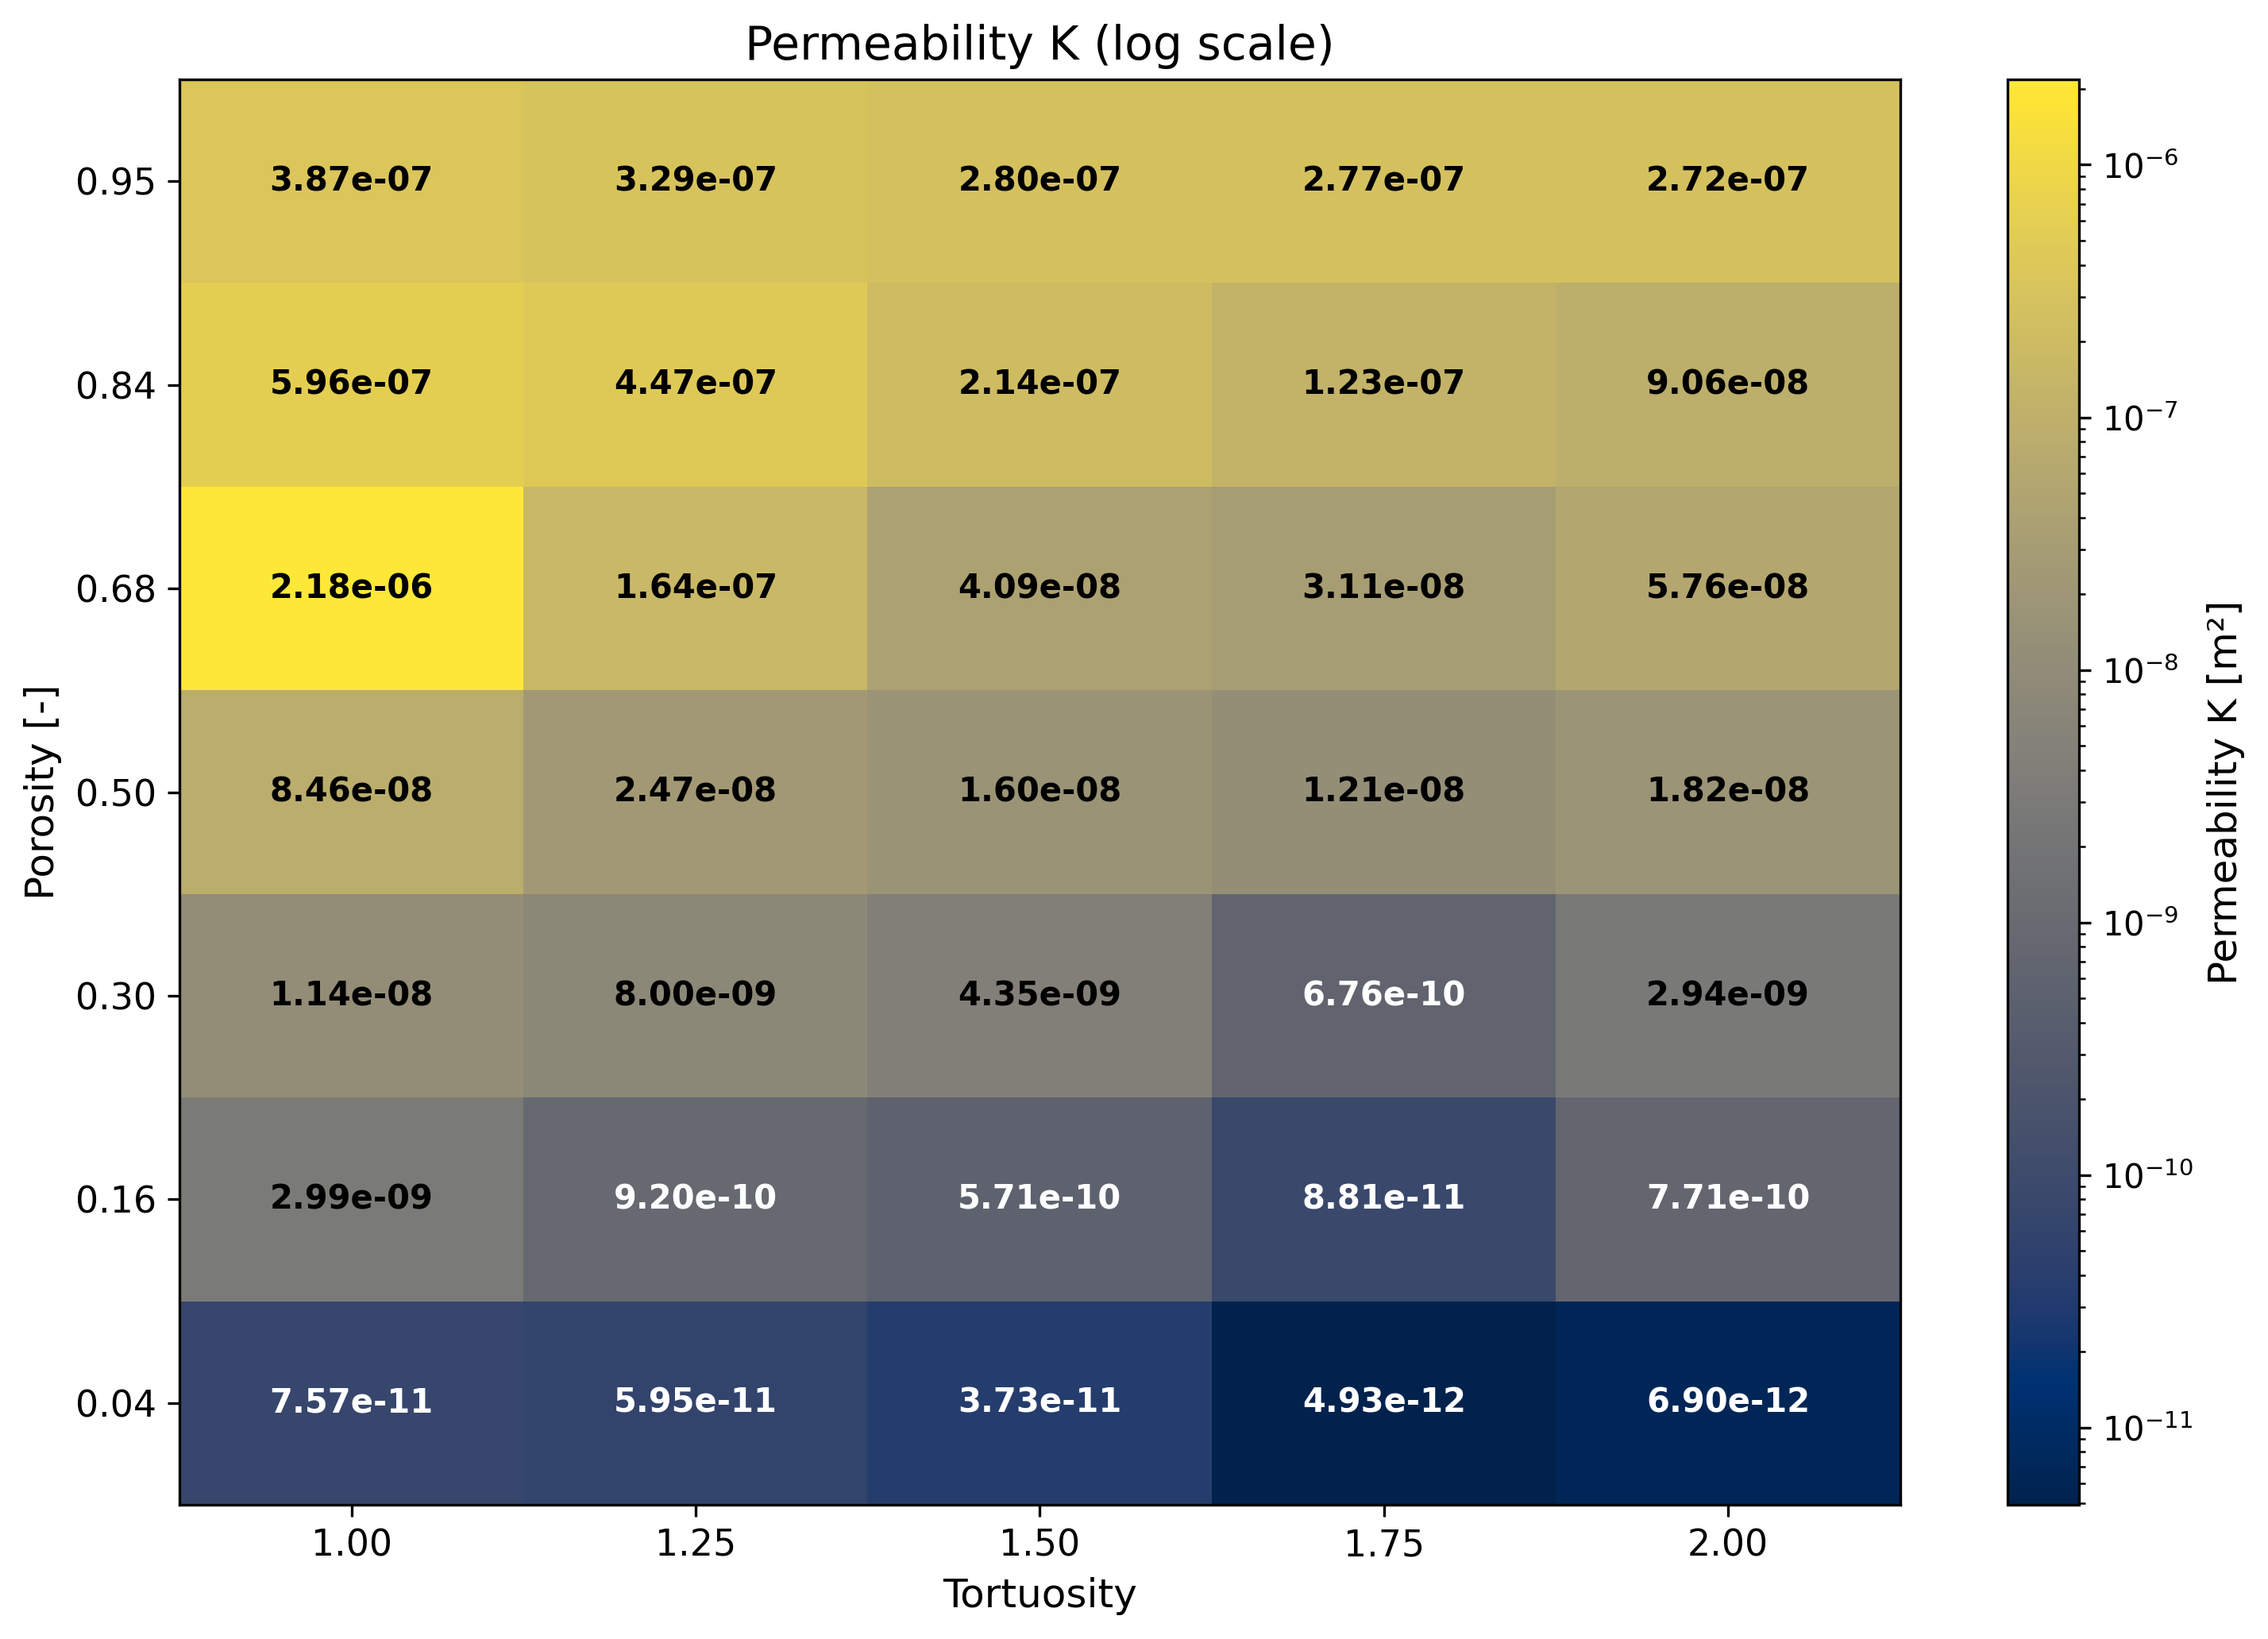
\includegraphics[width=11cm]{gr_perm.png}
    \caption{Permeability obtained for the investigated porous geometries as a
    function of porosity and tortuosity.}
    \label{fig:gr_perm}
\end{figure}

\clearpage

\begin{figure}[!ht]
    \centering
    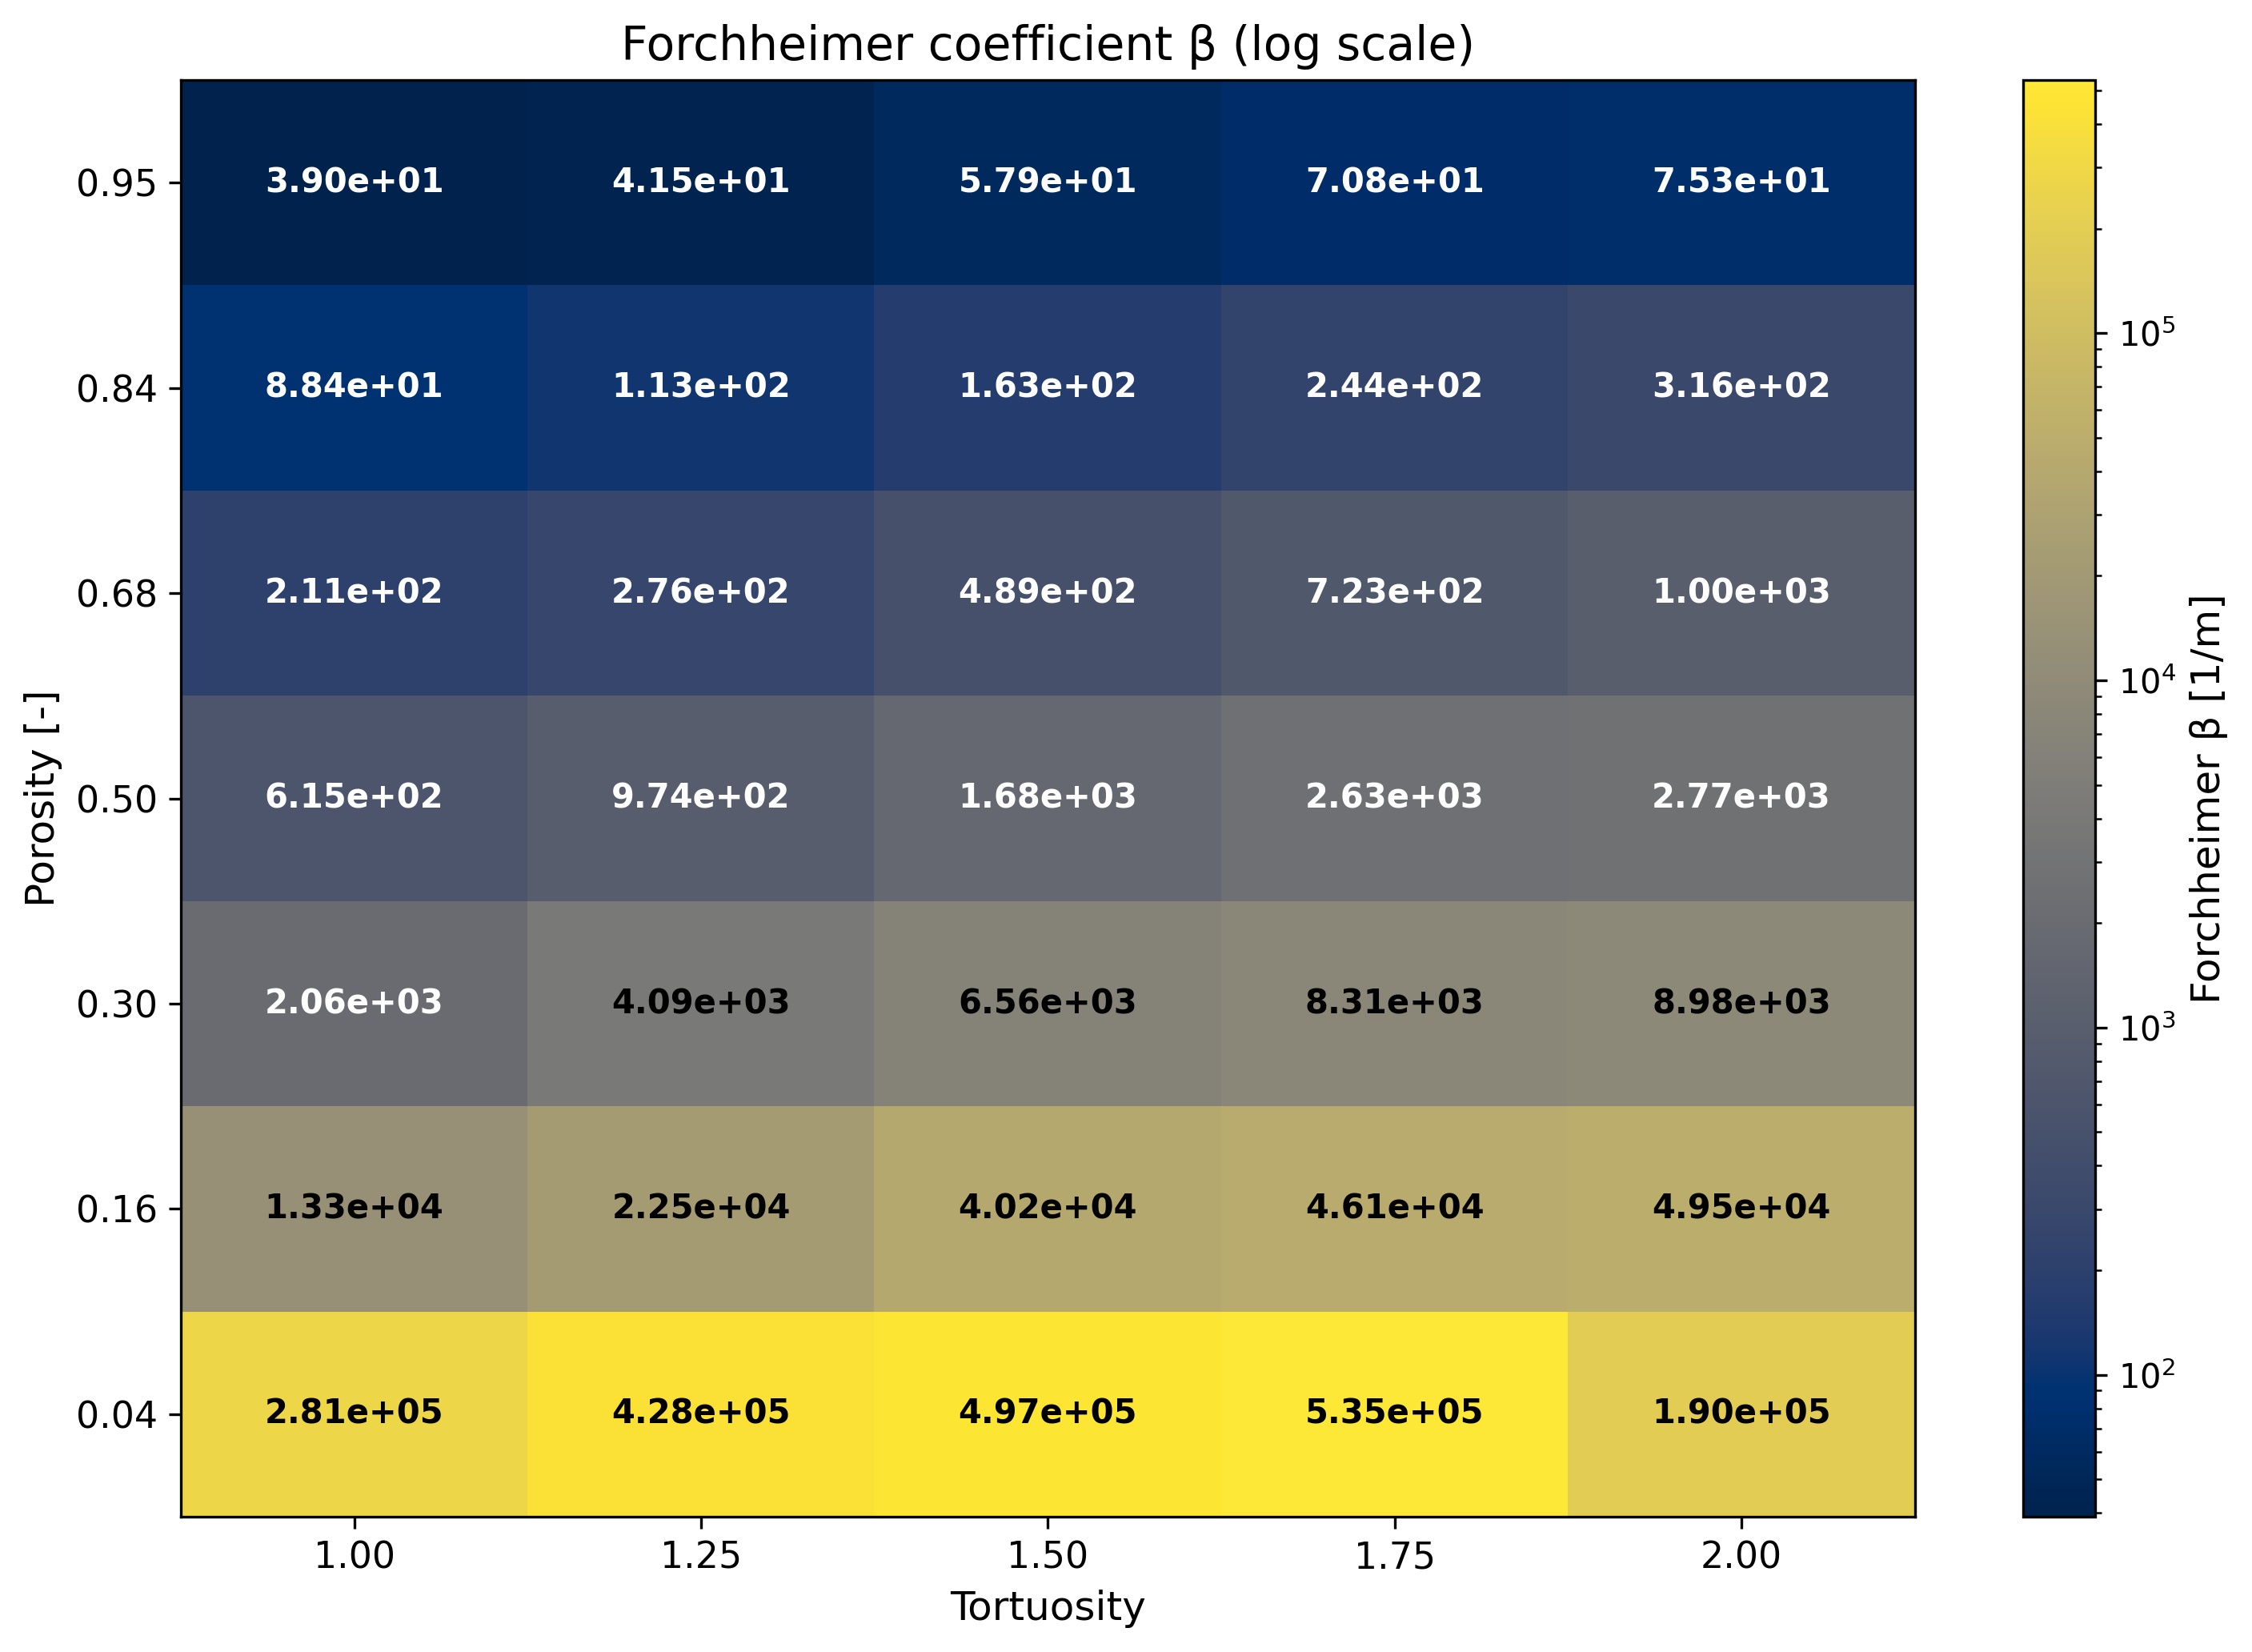
\includegraphics[width=11cm]{gr_forch_coeff.png}
    \caption{Forchheimer coefficient obtained for the investigated porous
    geometries as a function of porosity and tortuosity.}
    \label{fig:gr_forch}
\end{figure}

The variation visible in Figures~\ref{fig:gr_perm}
and~\ref{fig:gr_forch} covers several orders of magnitude. This is a direct
consequence of the exceptionally broad range of porous structures considered
in the parametric study. The investigated geometries extend from structures
with a very low void fraction to highly open porous media. Consequently, a
logarithmic representation of the hydraulic parameters was used in the
subsequent regression analysis.

The complete graphical results obtained for all evaluated tortuosity
definitions are provided in Appendix~1. The discussion in the present section
is focused on the tortuosity definition that produced the most representative
correlation with the hydraulic parameters.

\subsubsection{Three-dimensional representation of the parametric results}
\label{sec:parametric_3d_results}

To assess the combined influence of porosity and tortuosity, the calculated
hydraulic parameters were plotted in three-dimensional form. The resulting
distributions are shown in Figures~\ref{fig:gr_perm_3d}
and~\ref{fig:gr_forch_3d}.
\\
\\
The three-dimensional representations provide a comprehensive overview of the combined influence of porosity and tortuosity on the hydraulic behaviour of the investigated substitute porous structures. Rather than evaluating individual simulation cases separately, these response surfaces reveal the general trends governing fluid flow throughout the investigated design space. The permeability surface demonstrates the expected increase in permeability with increasing porosity, while the Forchheimer coefficient exhibits the opposite tendency, indicating a gradual reduction of inertial flow resistance in highly porous structures. Although tortuosity also affects both hydraulic parameters, its influence is generally less pronounced than that of porosity within the investigated range. It should be noted that the porosity values presented here correspond to the conventional volumetric porosity definition commonly adopted in the literature. In contrast, tortuosity does not possess a universally accepted definition, and several alternative geometric, hydraulic and transport-based formulations can be found in previous studies. Consequently, the tortuosity values reported in this work should be interpreted within the context of the definition adopted for the present substitute geometries and should not be directly compared with numerical values reported by other authors unless the same definition is employed.

\clearpage

\begin{figure}[!ht]
    \centering
    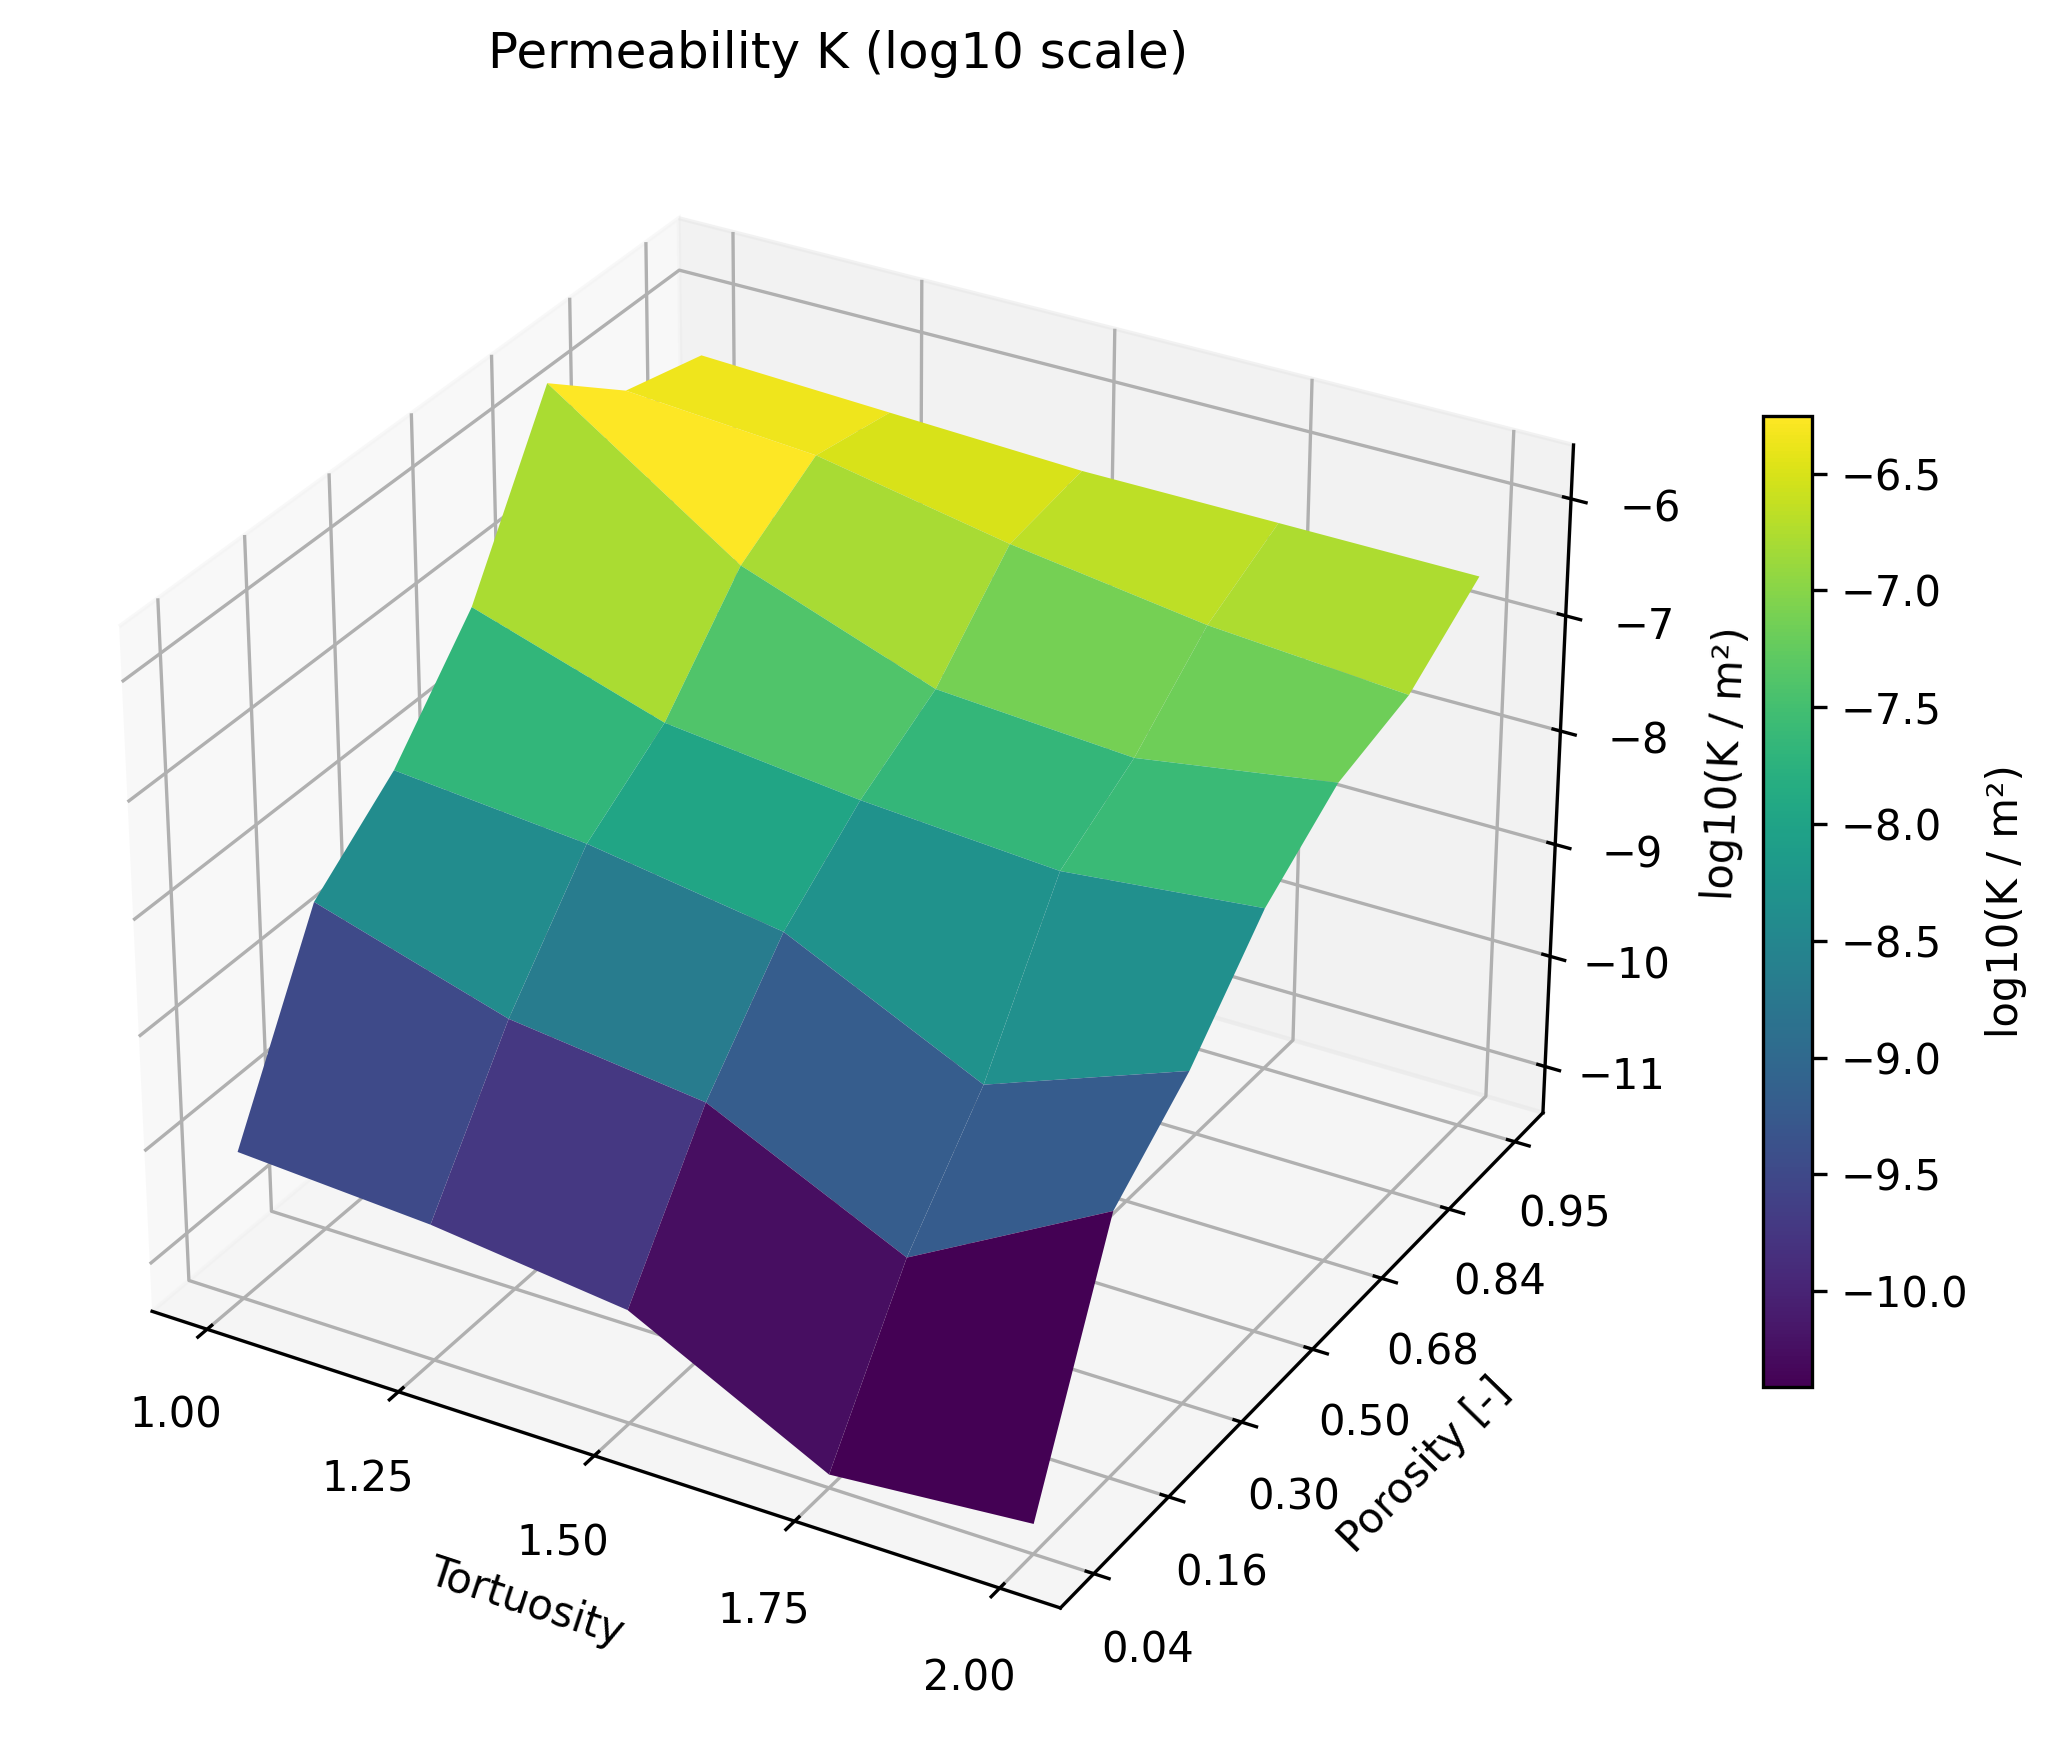
\includegraphics[width=11cm]{gr_perm_3d.png}
    \caption{Three-dimensional representation of permeability as a function of
    porosity and tortuosity.}
    \label{fig:gr_perm_3d}
\end{figure}

\begin{figure}[!ht]
    \centering
    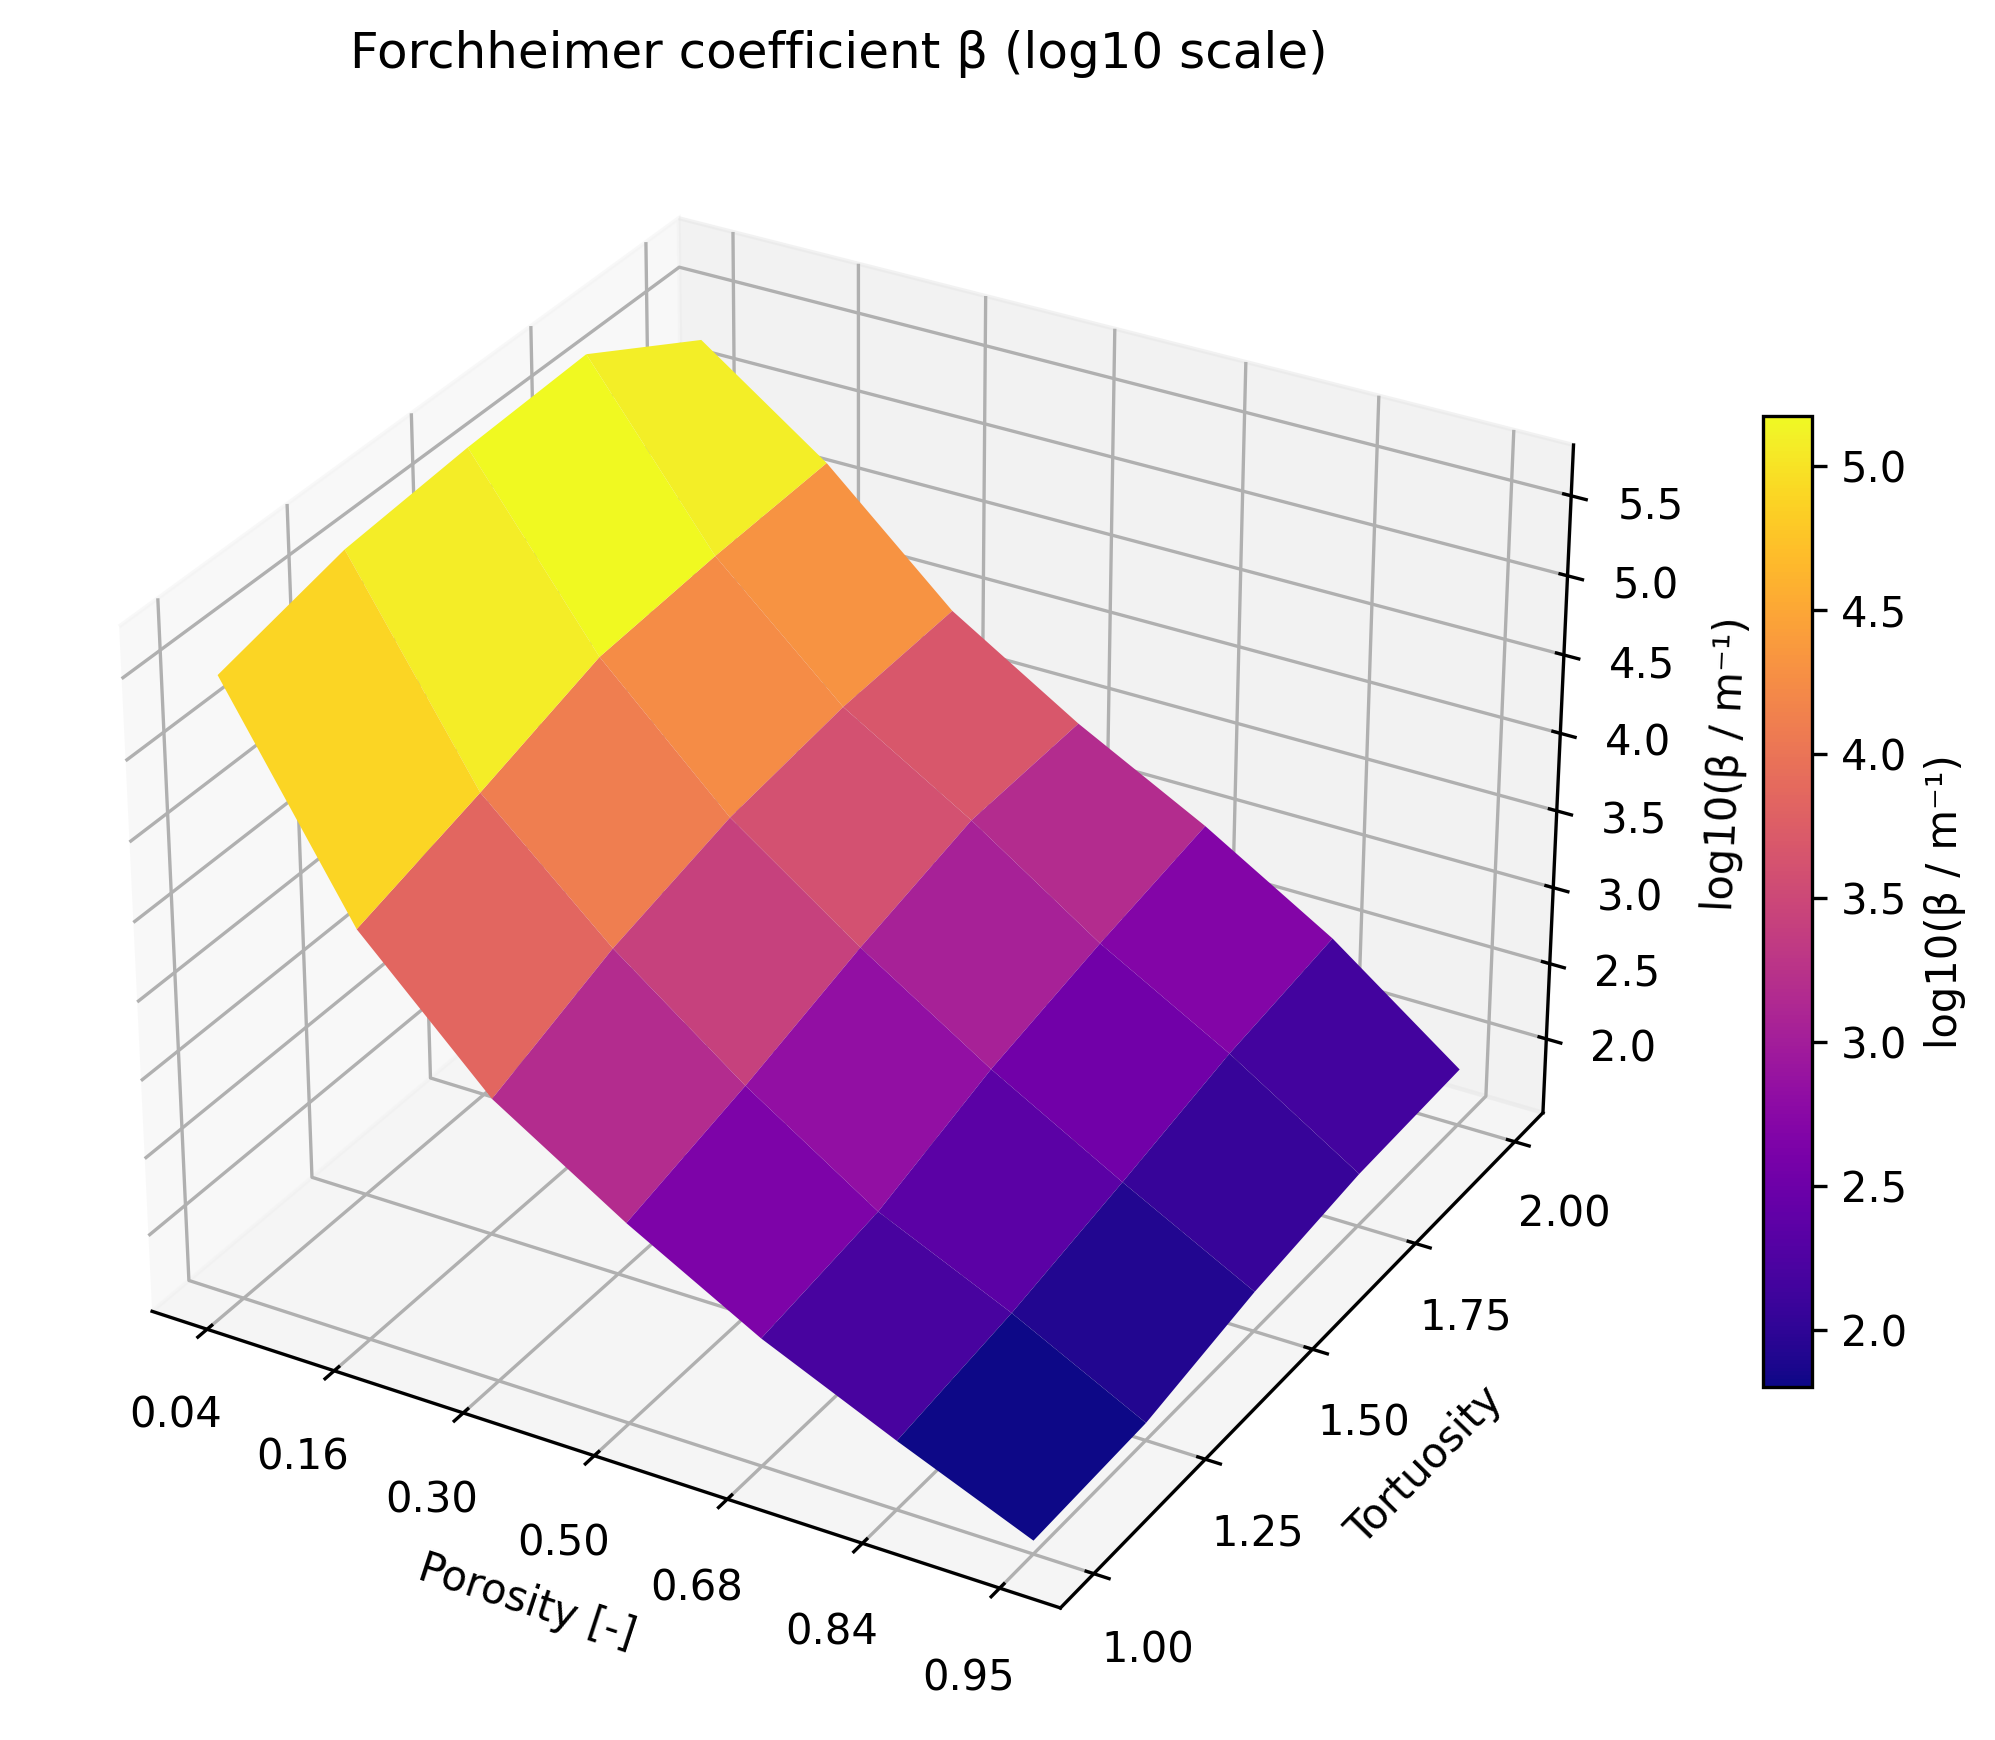
\includegraphics[width=11cm]{gr_forch_coeff_3d.png}
    \caption{Three-dimensional representation of the Forchheimer coefficient
    as a function of porosity and tortuosity.}
    \label{fig:gr_forch_3d}
\end{figure}

\clearpage

The three-dimensional plots confirm that neither porosity nor tortuosity alone
is sufficient to describe the complete variation in hydraulic behaviour.
Structures with comparable porosity may exhibit different permeability when
their flow paths differ in complexity. Similarly, geometries with comparable
tortuosity may produce different pressure losses because of differences in
their void fraction.

A multiple linear regression was first performed using the logarithms of the
hydraulic parameters as dependent variables and porosity and tortuosity as
independent variables. For permeability, the regression equation displayed in
the corresponding three-dimensional graph is

\begin{equation}
\log_{10}
\left(
\frac{K}{\mathrm{m^{2}}}
\right)
=
-8.734
-0.897\tau
+4.200\varepsilon.
\label{eq:permeability_logarithmic_plane}
\end{equation}

For the Forchheimer coefficient, the fitted regression plane is described by

\begin{equation}
\log_{10}
\left(
\frac{\beta}{\mathrm{m^{-1}}}
\right)
=
4.495
+0.488\tau
-3.749\varepsilon.
\label{eq:forchheimer_logarithmic_plane}
\end{equation}

These equations are convenient for statistical fitting and for visualising
the results as approximately planar surfaces. They can be rewritten directly
in terms of the predicted hydraulic parameters as

\begin{equation}
K
=
10^{-8.734-0.897\tau+4.200\varepsilon}
\;\mathrm{m^{2}},
\label{eq:permeability_exponential_form}
\end{equation}

and

\begin{equation}
\beta
=
10^{4.495+0.488\tau-3.749\varepsilon}
\;\mathrm{m^{-1}}.
\label{eq:forchheimer_exponential_form}
\end{equation}

Equations~\eqref{eq:permeability_exponential_form}
and~\eqref{eq:forchheimer_exponential_form} clearly show the direction of the
individual microstructural effects. An increase in porosity increases
permeability and decreases the Forchheimer coefficient. Conversely, an
increase in tortuosity decreases permeability and increases the Forchheimer
coefficient.

The positive effect of porosity on permeability is caused by the larger volume
available for fluid transport and by the reduced obstruction of the flow.
Higher tortuosity forces the fluid to travel along longer and more indirect
paths, thereby increasing viscous dissipation. In the case of the Forchheimer
coefficient, more tortuous and less porous geometries also promote stronger
local acceleration, deceleration, changes in flow direction and flow
separation. These mechanisms increase the nonlinear inertial contribution to
the pressure loss.

\subsubsection{Power-law correlations}
\label{sec:parametric_power_law_correlations}

Although the regression-plane representation is suitable for graphical
evaluation, hydraulic correlations for porous media are commonly expressed in
a power-law form. Such a representation allows the influence of the individual
microstructural parameters to be interpreted directly from their exponents.

Therefore, an additional regression was performed using logarithmic values of
both the dependent and independent variables. The general forms of the
correlations were defined as

\begin{equation}
K
=
C_{K}
\tau^{m_{K}}
\varepsilon^{n_{K}},
\label{eq:general_permeability_power_law}
\end{equation}

and

\begin{equation}
\beta
=
C_{\beta}
\tau^{m_{\beta}}
\varepsilon^{n_{\beta}}.
\label{eq:general_forchheimer_power_law}
\end{equation}

It should be emphasised that
Equations~\eqref{eq:general_permeability_power_law}
and~\eqref{eq:general_forchheimer_power_law} do not represent a purely
algebraic transformation of
Equations~\eqref{eq:permeability_logarithmic_plane}
and~\eqref{eq:forchheimer_logarithmic_plane}. The power-law equations result
from a separate regression in which $\log_{10}(\tau)$ and
$\log_{10}(\varepsilon)$ were used as explanatory variables.

The fitted surfaces and the corresponding power-law equations are presented
in Figures~\ref{fig:gr_perm_3d_fit} and~\ref{fig:gr_forch_3d_fit}.

\clearpage

\begin{figure}[!ht]
    \centering
    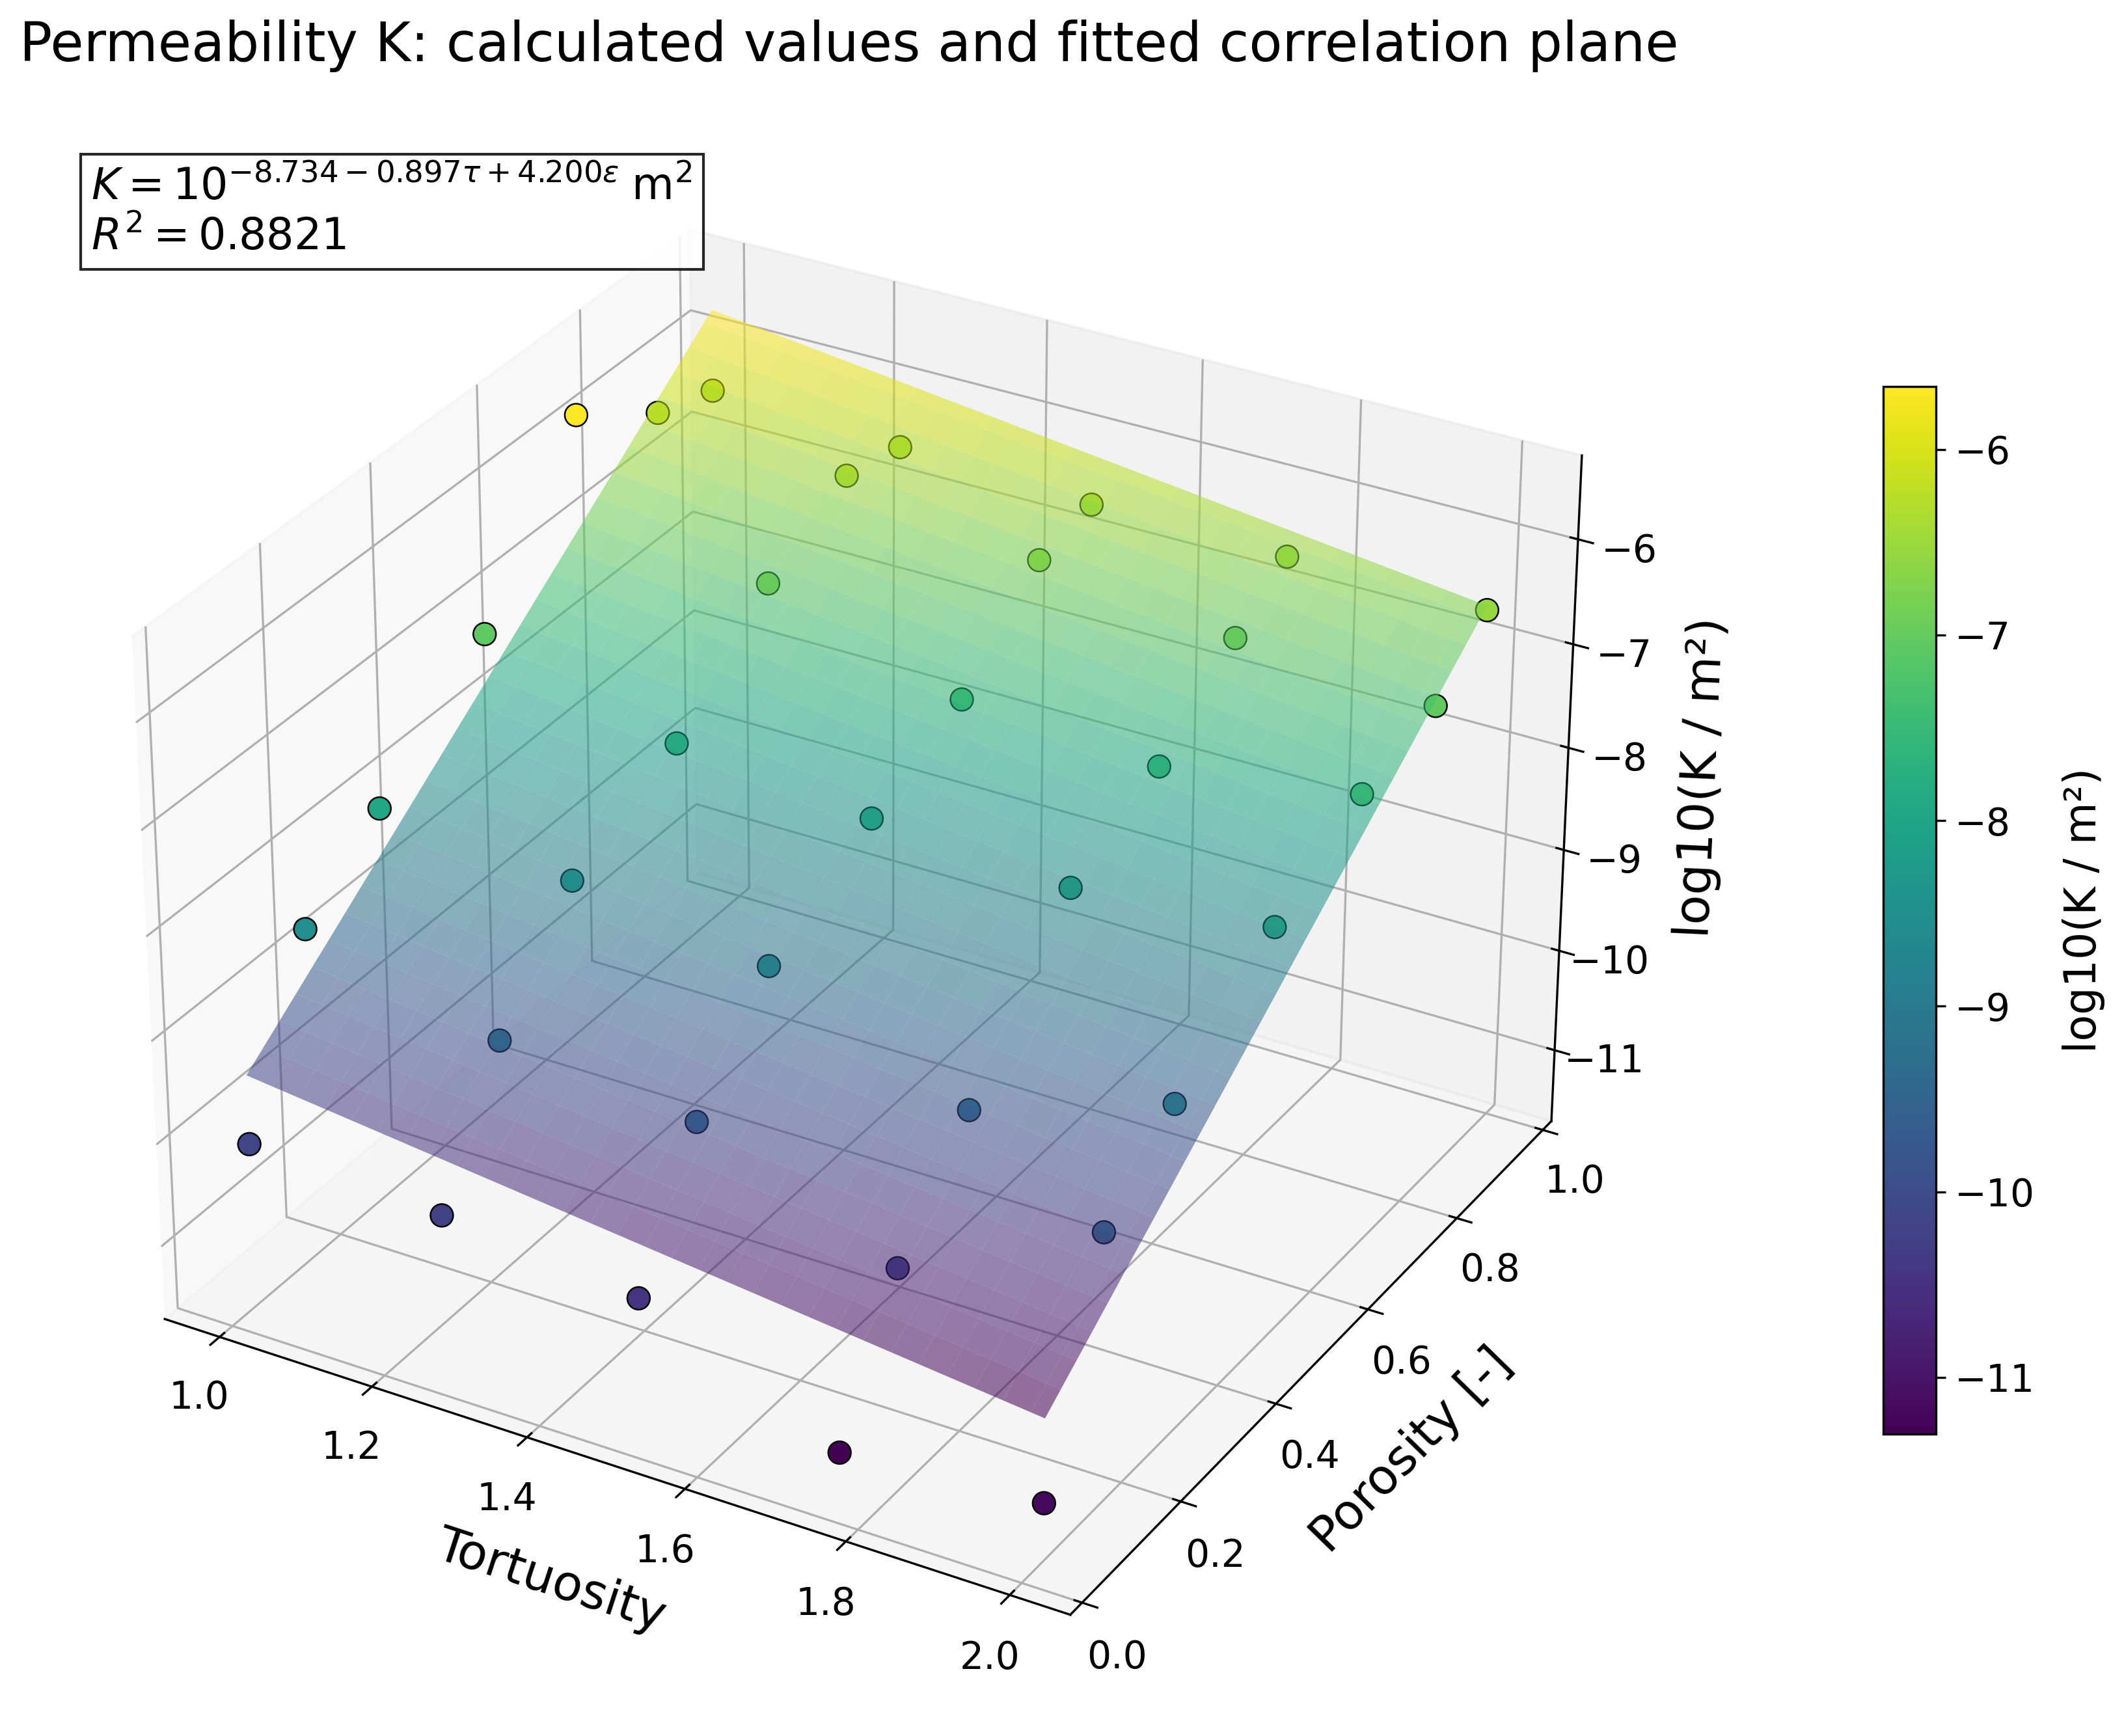
\includegraphics[width=12.2cm]{perm_FIT.png}
    \caption{Power-law fit of permeability as a function of porosity and
    tortuosity.}
    \label{fig:gr_perm_3d_fit}
\end{figure}

\begin{figure}[!ht]
    \centering
    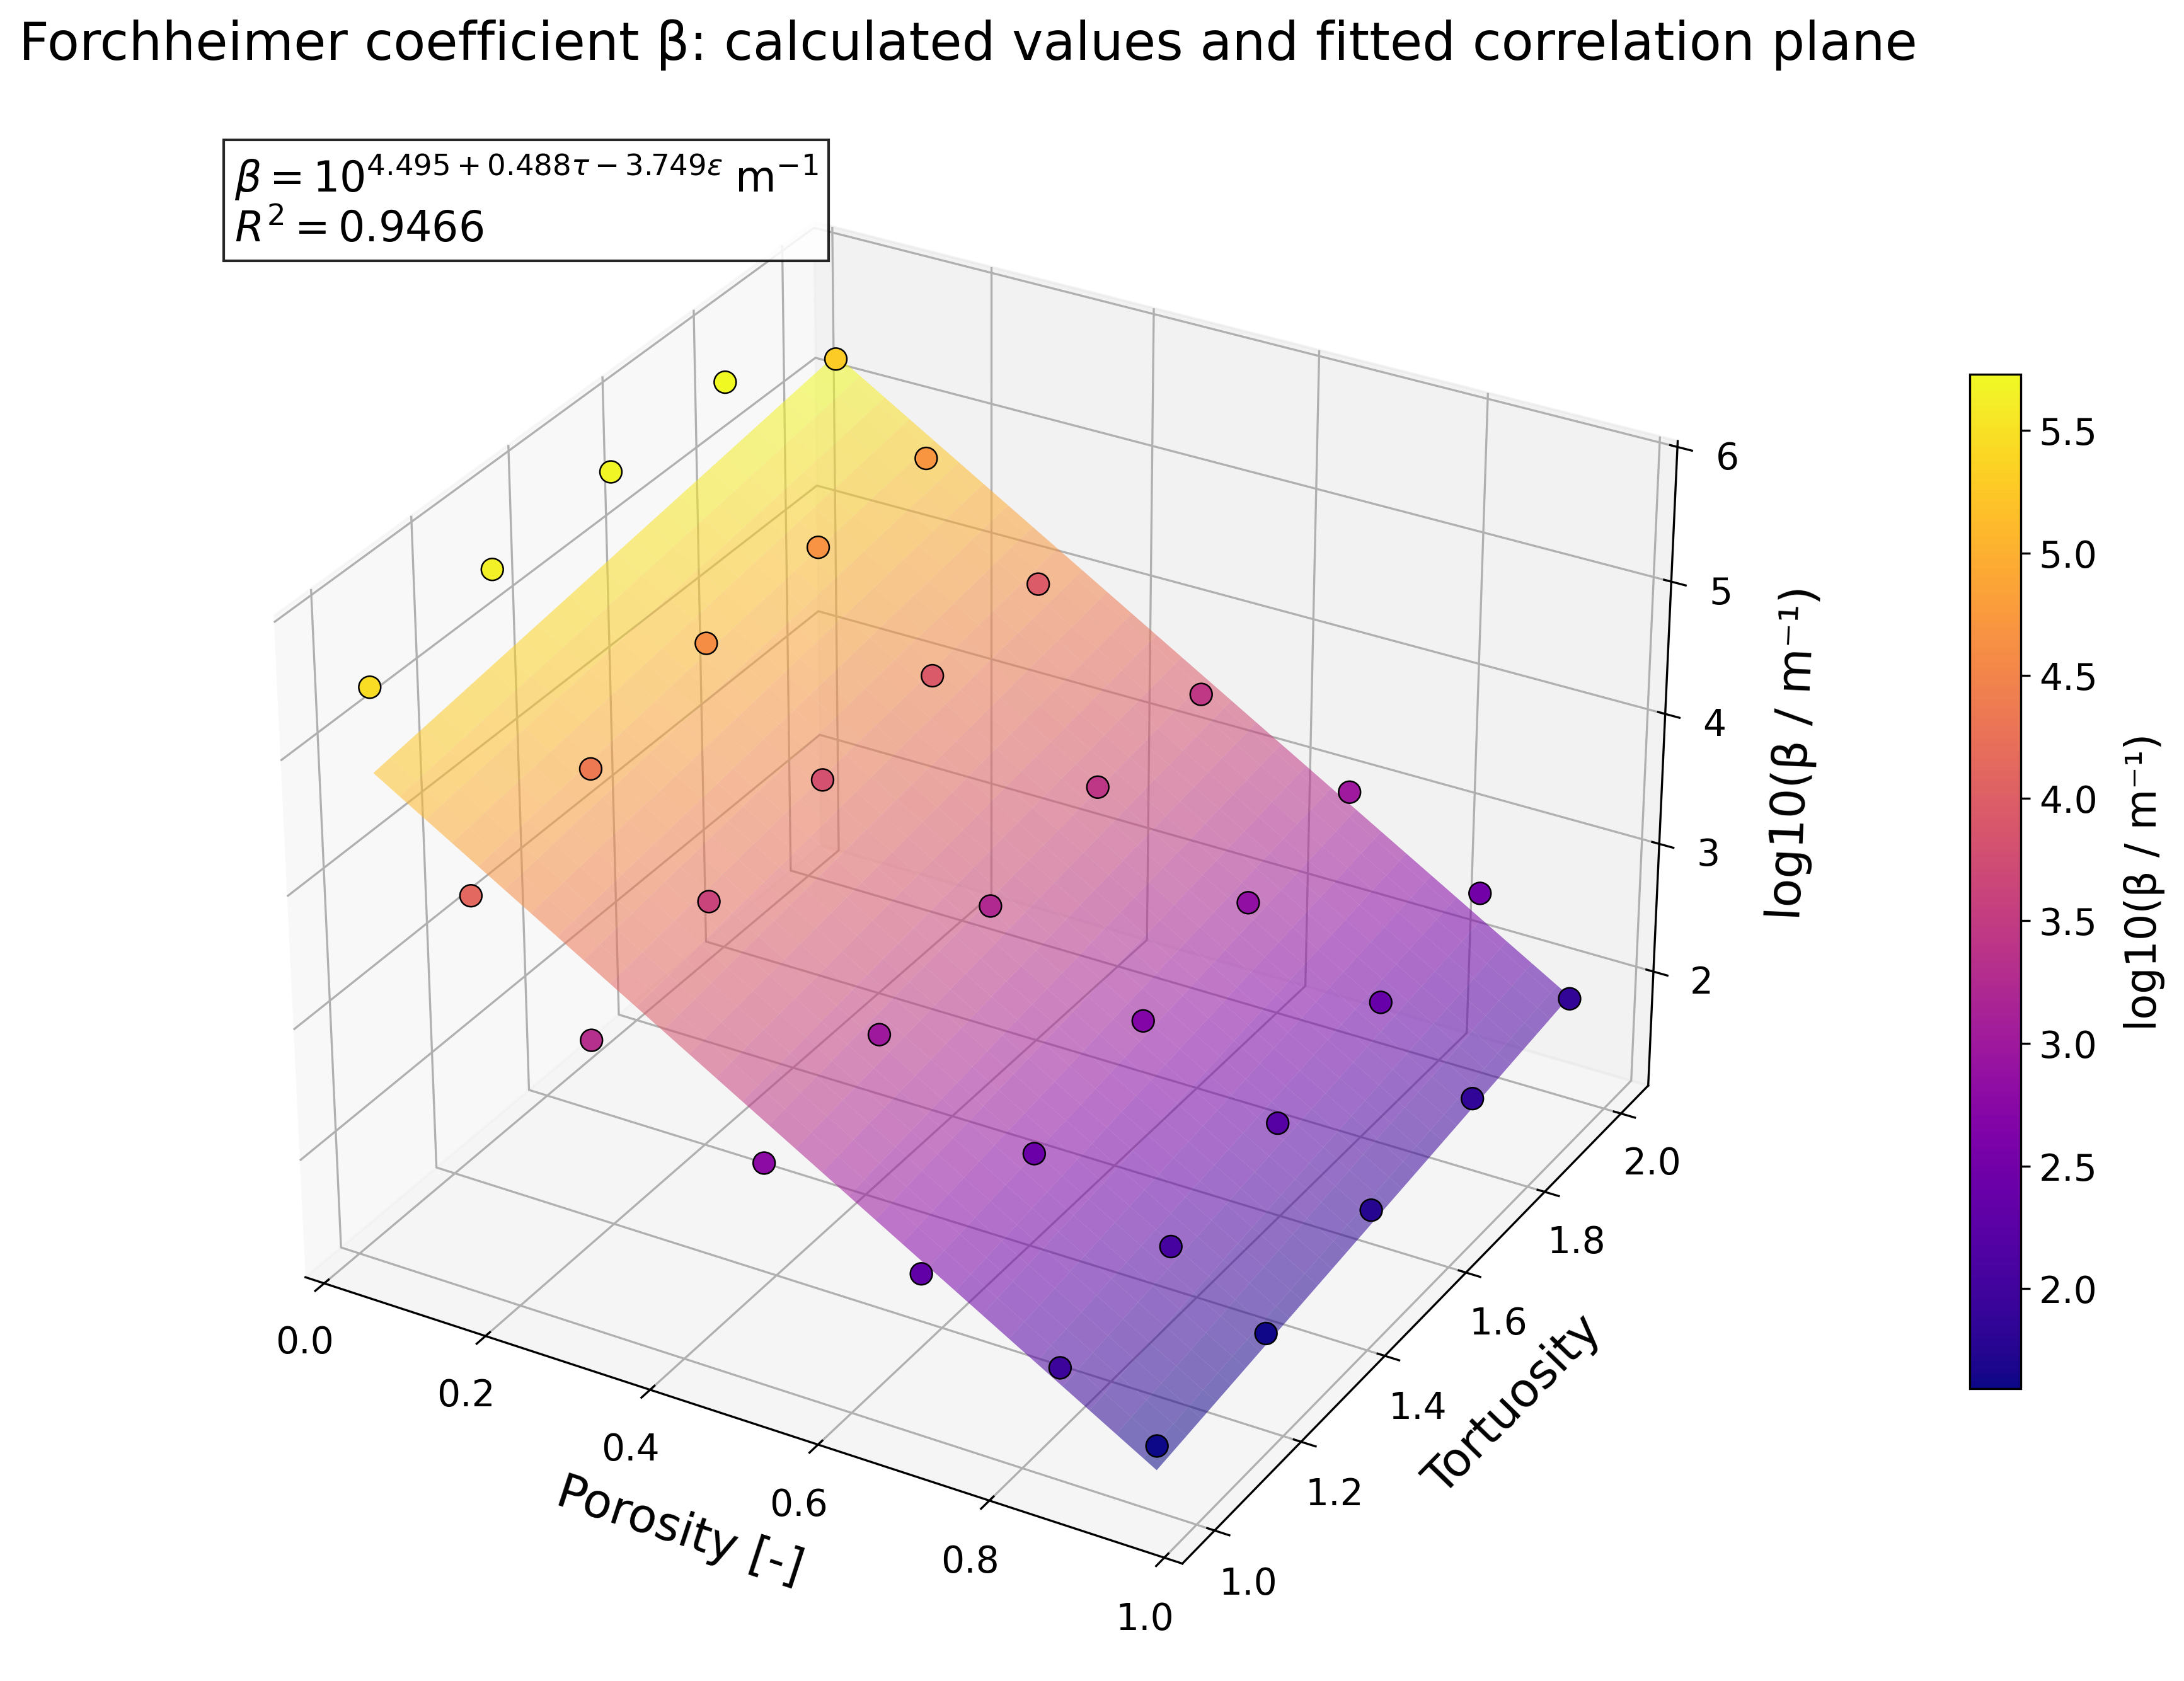
\includegraphics[width=12.2cm]{forch_fit.png}
    \caption{Power-law fit of the Forchheimer coefficient as a function of
    porosity and tortuosity.}
    \label{fig:gr_forch_3d_fit}
\end{figure}

\clearpage

The resulting permeability correlation is

\begin{equation}
\boxed{
K
=
9.439\times10^{-7}
\,\tau^{-3.091}
\,\varepsilon^{3.143}
\;\mathrm{m^{2}}
}
\label{eq:final_permeability_correlation}
\end{equation}

with a coefficient of determination evaluated in logarithmic space of

\begin{equation}
R^{2}_{\log K}
=
0.9531.
\label{eq:permeability_r_squared}
\end{equation}

The corresponding correlation for the Forchheimer coefficient is

\begin{equation}
\boxed{
\beta
=
6.801\times10^{1}
\,\tau^{1.661}
\,\varepsilon^{-2.709}
\;\mathrm{m^{-1}}
}
\label{eq:final_forchheimer_correlation}
\end{equation}

with

\begin{equation}
R^{2}_{\log\beta}
=
0.9549.
\label{eq:forchheimer_r_squared}
\end{equation}

The coefficients of determination show that the two microstructural parameters
explain a substantial proportion of the variation in both hydraulic
quantities. This is particularly important considering the diversity of the
investigated geometries and the wide ranges of porosity, tortuosity,
permeability and inertial resistance represented in the dataset.

\subsubsection{Interpretation of the permeability correlation}
\label{sec:interpretation_permeability_correlation}

The permeability correlation can be written proportionally as

\begin{equation}
K
\propto
\tau^{-3.091}
\varepsilon^{3.143}.
\label{eq:permeability_proportional_form}
\end{equation}

The positive porosity exponent confirms the strong increase in permeability
with increasing void fraction. The obtained exponent,

\begin{equation}
n_{K}
=
3.143,
\end{equation}

is close to the cubic dependence on porosity appearing in the classical
Kozeny--Carman equation. In a commonly used form, the Kozeny--Carman
relationship may be written as

\begin{equation}
K
=
\frac{\varepsilon^{3}}
{C_{\mathrm{KC}}\tau^{2}S_{v}^{2}},
\label{eq:kozeny_carman_comparison}
\end{equation}

where $C_{\mathrm{KC}}$ is the Kozeny--Carman coefficient and $S_{v}$ is the
specific surface area of the porous structure
\cite{XuYu2008,Costa2006}.

The exponent of $3.143$ obtained in the present work is therefore consistent
with the characteristic cubic dependence predicted by
Kozeny--Carman-type models. This agreement is notable because the investigated
dataset does not consist of small variations of a single porous structure.
Instead, it contains geometries with strongly different void fractions and
flow-path configurations.

Nevertheless, the agreement of the porosity exponent with the cubic term
should not be interpreted as complete validation of the classical
Kozeny--Carman equation. The classical relationship contains additional
microstructural parameters, particularly specific surface area, and is often
supplemented by terms involving the solid fraction or a characteristic pore
diameter. In the present regression, the effects of these parameters are not
included explicitly and may therefore be partly incorporated into the fitted
coefficient and exponents.

The tortuosity exponent in
Equation~\eqref{eq:final_permeability_correlation} is

\begin{equation}
m_{K}
=
-3.091.
\end{equation}

Its negative sign is physically consistent with the expected influence of
tortuosity. A higher tortuosity corresponds to a longer and more complicated
flow path through the porous material. The fluid is therefore exposed to a
larger effective flow length and greater viscous dissipation, resulting in a
reduction in permeability.

The classical Kozeny--Carman formulation commonly includes an inverse
quadratic tortuosity dependence,

\begin{equation}
K
\propto
\tau^{-2}.
\end{equation}

The dependence obtained in the present study,

\begin{equation}
K
\propto
\tau^{-3.091},
\end{equation}

is somewhat stronger. This difference is plausible because the image-derived
tortuosity may reflect not only the increase in the mean flow-path length but
also other correlated structural effects. These may include pore
constrictions, changes in local flow direction, reduced pore connectivity and
variations in the cross-sectional area available for flow.

Moreover, porosity, tortuosity, pore size and specific surface area are not
fully independent descriptors. Because only porosity and tortuosity were
included in the present correlation, their fitted exponents may partly capture
the influence of other microstructural quantities. Consequently, the exponent
$-3.091$ should be regarded as an effective empirical value for the
investigated set of structures rather than as a universal theoretical
constant.

\subsubsection{Interpretation of the Forchheimer coefficient correlation}
\label{sec:interpretation_forchheimer_correlation}

The fitted Forchheimer correlation may be expressed proportionally as

\begin{equation}
\beta
\propto
\tau^{1.661}
\varepsilon^{-2.709}.
\label{eq:forchheimer_proportional_form}
\end{equation}

The positive tortuosity exponent,

\begin{equation}
m_{\beta}
=
1.661,
\end{equation}

indicates that inertial resistance increases with increasing flow-path
complexity. This trend is physically reasonable. In a highly tortuous porous
medium, the fluid repeatedly changes direction and passes through constricted
regions. This promotes local acceleration and deceleration, flow separation,
recirculation and momentum exchange with the solid structure. These phenomena
increase form drag and therefore increase the nonlinear contribution to the
pressure loss.

The negative porosity exponent,

\begin{equation}
n_{\beta}
=
-2.709,
\end{equation}

shows that the Forchheimer coefficient decreases strongly with increasing
porosity. A structure with lower porosity contains a larger fraction of solid
material and generally provides narrower flow passages. For a given
superficial velocity, the local pore velocity is consequently higher, and the
fluid interacts more intensively with the solid skeleton. Both effects
contribute to an increase in inertial pressure losses.

The signs of the obtained exponents agree with established descriptions of
non-Darcy flow in porous media. Published correlations commonly express the
Forchheimer coefficient as an inverse function of porosity and permeability
and as an increasing function of geometrical complexity. A general form may be
written as

\begin{equation}
\beta
=
\frac{C_{1}\tau^{a}}
{K^{b}\varepsilon^{c}},
\label{eq:general_literature_forchheimer}
\end{equation}

where the empirical constants and exponents depend on the investigated
material and the definition of the characteristic length
\cite{Yang2021}.

Direct numerical agreement between published Forchheimer correlations and
Equation~\eqref{eq:final_forchheimer_correlation} cannot be expected. Many
existing models were derived for a specific class of porous media, such as
packed beds or highly porous open-cell metal foams, and frequently contain an
explicit pore diameter, ligament diameter or specific surface area. By
contrast, the present correlation was developed using only porosity and
tortuosity and was fitted to a much broader range of structures.

The logarithmic coefficient of determination,

\begin{equation}
R^{2}_{\log\beta}
=
0.9549,
\end{equation}

therefore represents a strong result. It demonstrates that the simple
two-parameter power law captures most of the observed variation in inertial
resistance, despite the absence of an explicit characteristic pore dimension.

\subsubsection{Applicability and limitations of the proposed correlations}
\label{sec:correlation_applicability}

The correlations obtained in the present study are empirical and their
dimensional coefficients are valid for the units used in
Equations~\eqref{eq:final_permeability_correlation}
and~\eqref{eq:final_forchheimer_correlation}. Permeability must be expressed in
$\mathrm{m^{2}}$, the Forchheimer coefficient in $\mathrm{m^{-1}}$, and both
porosity and tortuosity must be entered as dimensionless quantities.

The correlations should primarily be applied within the range of
microstructural parameters represented by the investigated dataset. Their
extrapolation beyond this range requires additional validation. The definition
and method used for determining tortuosity must also remain consistent, because
different geometrical, hydraulic and diffusive definitions of tortuosity may
produce different numerical values.

The complete results obtained using all evaluated tortuosity definitions,
including the corresponding graphical comparisons and regression results, are
provided in Appendix~1.

Other microstructural parameters could potentially improve the predictive
accuracy. These include characteristic pore diameter, pore-throat diameter,
specific surface area, ligament diameter, pore-size distribution, connectivity
and anisotropy. However, the main purpose of the present correlations is to
determine whether parameters accessible from optical image analysis can be
used to estimate hydraulic behaviour before direct testing.

From this perspective, the obtained results are promising. Porosity and
tortuosity alone provide coefficients of determination exceeding $0.95$ in
logarithmic space for both permeability and the Forchheimer coefficient. The
correlations may therefore serve as a first engineering estimate of the
hydraulic characteristics of an unknown porous sample based on its observed
microstructure.

\subsubsection{Parametric study conclusion}
\label{sec:parametric_study_conclusion}

The parametric study demonstrated a clear relationship between the
microstructure of porous materials and their hydraulic behaviour. Increasing
porosity resulted in higher permeability and a lower Forchheimer coefficient,
whereas increasing tortuosity produced lower permeability and higher inertial
resistance.

Two complementary correlation forms were obtained. The regression-plane
equations,

\begin{equation}
K
=
10^{-8.734-0.897\tau+4.200\varepsilon}
\;\mathrm{m^{2}},
\end{equation}

and

\begin{equation}
\beta
=
10^{4.495+0.488\tau-3.749\varepsilon}
\;\mathrm{m^{-1}},
\end{equation}

directly describe the fitted surfaces displayed in the three-dimensional
graphs. The independently fitted power-law correlations,

\begin{equation}
K
=
9.439\times10^{-7}
\,\tau^{-3.091}
\,\varepsilon^{3.143}
\;\mathrm{m^{2}},
\end{equation}

and

\begin{equation}
\beta
=
6.801\times10^{1}
\,\tau^{1.661}
\,\varepsilon^{-2.709}
\;\mathrm{m^{-1}},
\end{equation}

provide a more readily interpretable engineering representation.

The permeability exponent associated with porosity, $3.143$, is close to the
cubic dependence appearing in classical Kozeny--Carman-type models. The
tortuosity exponent of $-3.091$ indicates a stronger sensitivity than the
inverse quadratic dependence commonly assumed in the classical formulation,
but it retains the physically expected trend. For the Forchheimer coefficient,
the positive tortuosity exponent and negative porosity exponent are consistent
with the increase in inertial losses caused by more complicated and more
constricted flow paths.

The principal significance of the obtained correlations lies in the
exceptionally broad porosity range covered by the parametric study,

\begin{equation}
0.043
\leq
\varepsilon
\leq
0.954.
\label{eq:parametric_porosity_range}
\end{equation}

This interval extends from very dense structures with a small void fraction to
highly open porous media. Many published correlations are derived and
validated for a considerably narrower range and frequently for only one
specific class of porous material. Correlations developed for open-cell metal
foams, for example, are typically assessed predominantly within the
high-porosity region.

Despite this broad interval and the substantial geometrical diversity of the
investigated structures, the proposed correlations achieved

\begin{equation}
R^{2}_{\log K}
=
0.9531
\qquad\text{and}\qquad
R^{2}_{\log\beta}
=
0.9549.
\end{equation}

The correlations therefore describe not only small variations among
geometrically similar samples but a heterogeneous set of porous structures
covering almost the entire practically relevant porosity scale. Exact
agreement with coefficients reported for an individual material class should
consequently not be expected. The fitted exponents represent effective
dependencies across a substantially wider range of structures.

The combination of physically consistent trends, high coefficients of
determination and an exceptionally broad porosity interval supports the
conclusion that optical microstructural parameters can be used to provide a
useful preliminary estimate of permeability and the Forchheimer coefficient
before a porous material is tested hydraulically.


\newpage
\section{The experimental measurements of porous samples}

\subsection{Experimental facility TEALC}
The Thermohydraulic Experiment for Advanced Liquid Cooling (TEALC) facility was designed and built within the present doctoral work to characterize the hydraulic and thermal behaviour of water-cooled test sections under controlled boundary conditions. The modular test section accepts samples up to 300~mm in length and enables pressure-drop and temperature measurements over a range of coolant flow rates.

\subsubsection{Objectives}
The facility is used to determine pressure loss as a function of coolant flow rate, evaluate heat-removal performance where applicable, quantify the influence of operating conditions, and provide experimental data for validation of computational fluid dynamics (CFD) models.

\subsubsection{Device schematics}
Figure~\ref{fig:tealc_scheme} shows the experimental loop. A reservoir and expansion volume stabilize the circuit, while the pump establishes the required flow. The test section is instrumented for pressure-drop and temperature measurements; a cooler and electric heater provide control of the coolant inlet condition.

\begin{figure}[ht!]
  \centering
  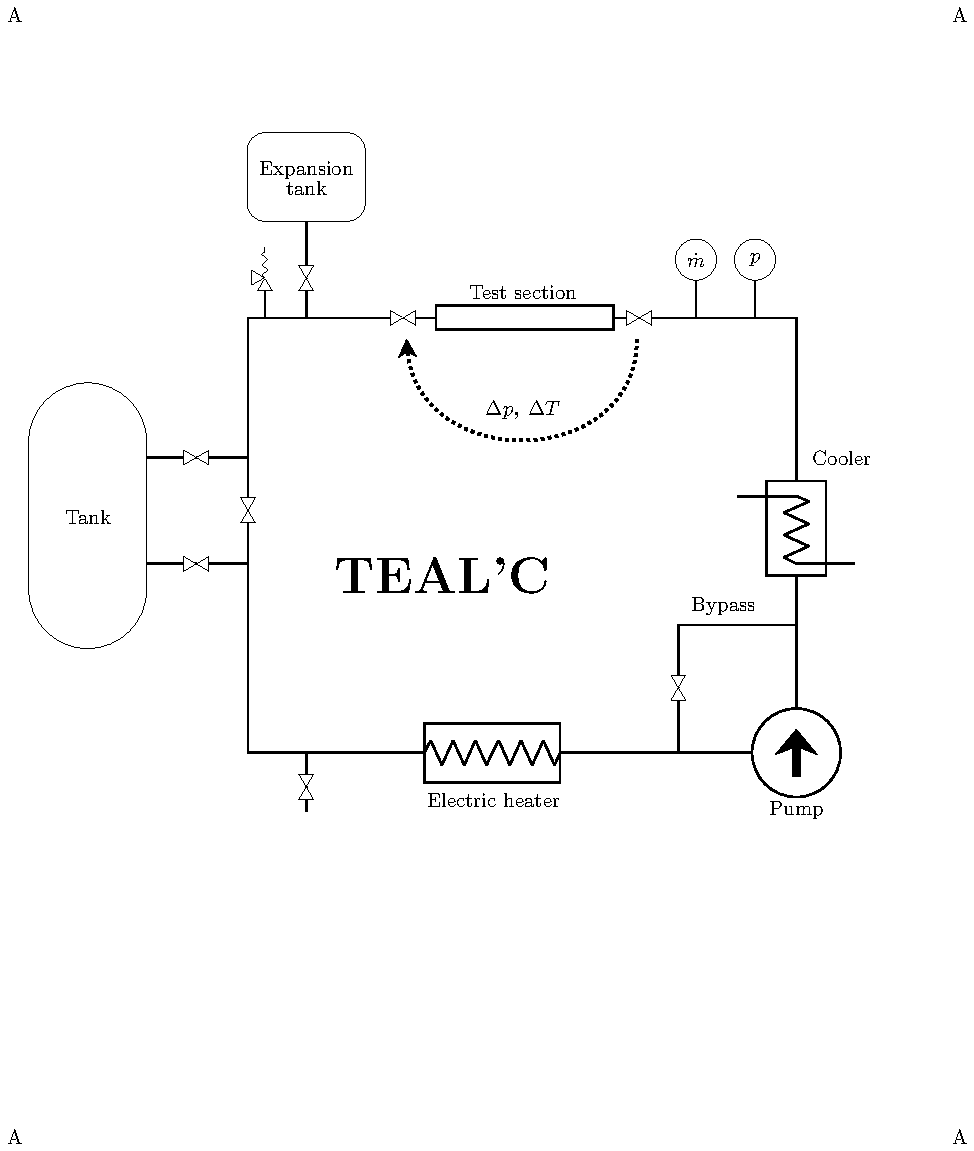
\includegraphics[width=13cm]{schema_smycky.pdf}
  \caption{TEALC experimental device schematic.}
  \label{fig:tealc_scheme}
\end{figure}

The principal operating parameters used in this work are summarized in Table~\ref{tab:tealc_parameters}.

\begin{table}[ht!]
  \centering
  \begin{tabular}{|l|c|}
    \hline
    Maximum coolant pressure & 10~bar \\
    \hline
    Coolant & Water \\
    \hline
    Maximum coolant velocity & 5~m/s \\
    \hline
    Total pipe length & approximately 10~m \\
    \hline
    Nominal inlet coolant temperature & 25~$^\circ$C \\
    \hline
  \end{tabular}
  \caption{Principal TEALC experimental device parameters.}
  \label{tab:tealc_parameters}
\end{table}

The experimental setup is designed to evaluate the hydraulic performance of various porous material samples. The setup consists of the TEALC experimental loop, through which water is circulated under controlled flow conditions. To obtain a comprehensive dataset, a wide range of porous samples with different materials and pore structures was collected and tested. Since the primary objective of this work is to investigate the hydraulic behaviour of porous media, heat transfer was not considered. Consequently, samples made of metallic, ceramic, and polymeric materials could be examined under identical hydraulic conditions. Instead, particular emphasis was placed on optical microscopy and microstructural characterization to establish the relationship between pore morphology and the measured hydraulic performance.

\subsection{Material sample analysis - porous structures}
This chapter introduces the porous foam samples investigated in this study and the experimental methodology used for their characterization. Optical microscopy was performed to examine the pore morphology, and the resulting images were used to evaluate the pore size distribution based on the equivalent circular diameter. The measurement procedure and image analysis methodology are described first, followed by an overview of the investigated samples together with their main parameters. Finally, representative optical micrographs of each sample are presented and discussed.
\subsubsection{Microstructure analysis methodology}
\label{sec:pore_size}

Pore size was evaluated from surface images using ImageJ/Fiji. Before the analysis, each image was calibrated using the scale bar. Since the contrast between the solid material and the pore cavities was not sufficiently uniform, the pores were outlined manually. Each continuous cavity surrounded by the solid phase was considered as one pore, while pores with unclear boundaries or intersecting the image boundary were excluded from the analysis.

Figure \ref{fig:pore_detection} shows an example of a processed image with manually identified pore boundaries used for the evaluation.

\begin{figure}[htbp]
    \centering
    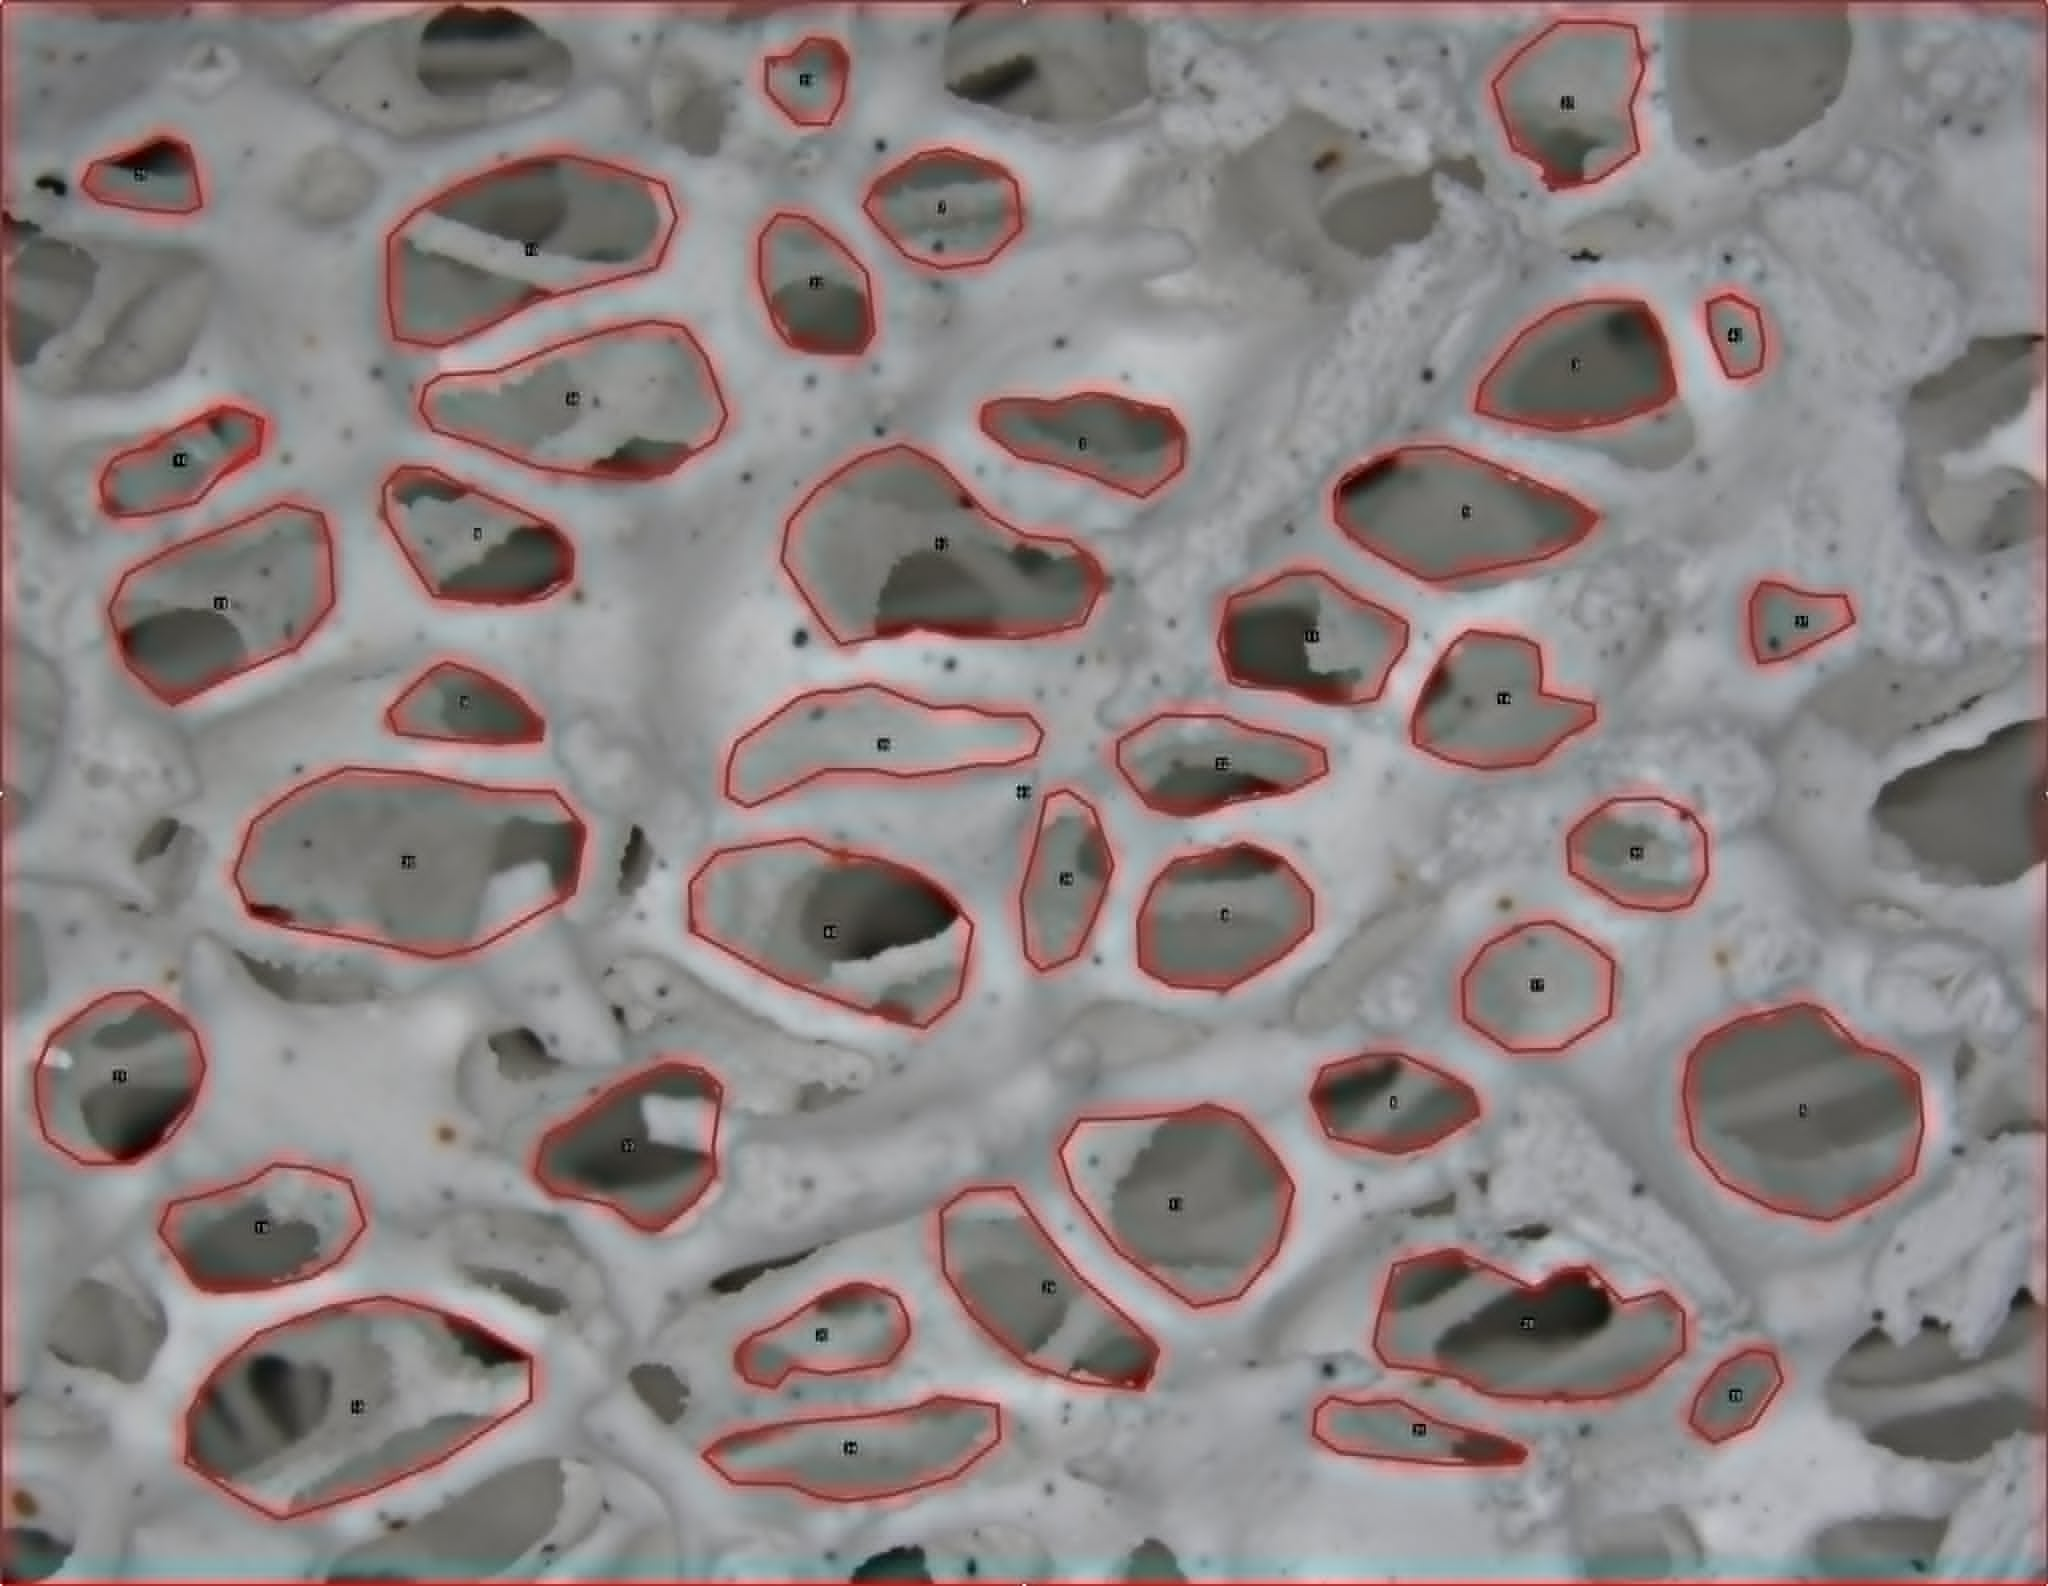
\includegraphics[width=0.5\textwidth]{mereni_bety_2.jpg}
    \caption{Example of manually identified pore boundaries used for pore size evaluation.}
    \label{fig:pore_detection}
\end{figure}

The area of each selected pore, $A$, was measured and converted into the equivalent circular diameter, $d_{\mathrm{e}}$, defined as the diameter of a circle having the same area as the analysed pore,

\begin{equation}
d_{\mathrm{e}}
=
\sqrt{\frac{4A}{\pi}}
\label{eq:equivalent_circular_diameter}
\end{equation}

where $A$ is the pore area expressed in $\mathrm{mm^2}$. The equivalent circular diameter provides a single characteristic dimension for comparing pores of irregular shape. Figure \ref{fig:pore_deq} illustrates the equivalent circular diameter and the Ferret minimum and maximum diameters, which are defined as the smallest and largest distances between two parallel lines tangent to the pore boundary. The equivalent circular diameter is always smaller than the Ferret maximum diameter and larger than the Ferret minimum diameter, providing a more representative measure of the pore size for irregularly shaped pores.

\begin{figure}[htbp]
    \centering
    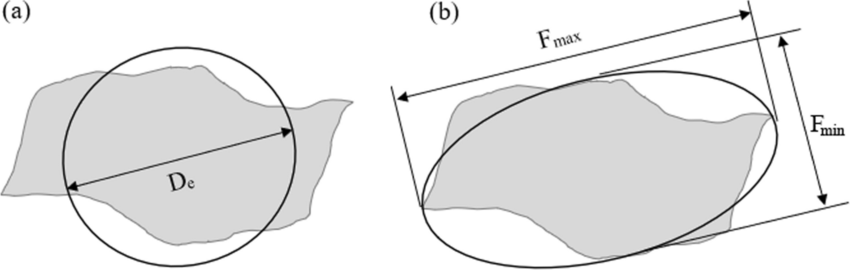
\includegraphics[width=0.7\textwidth]{deq_schema.png}
    \caption{Schematic representation of the equivalent circular diameter and Ferret min and max diameters \cite{Qiu2023}.}
    \label{fig:pore_deq}
\end{figure}

The equivalent circular diameters obtained from all analysed pores were statistically evaluated. 

\begin{figure}[htbp]
    \centering
    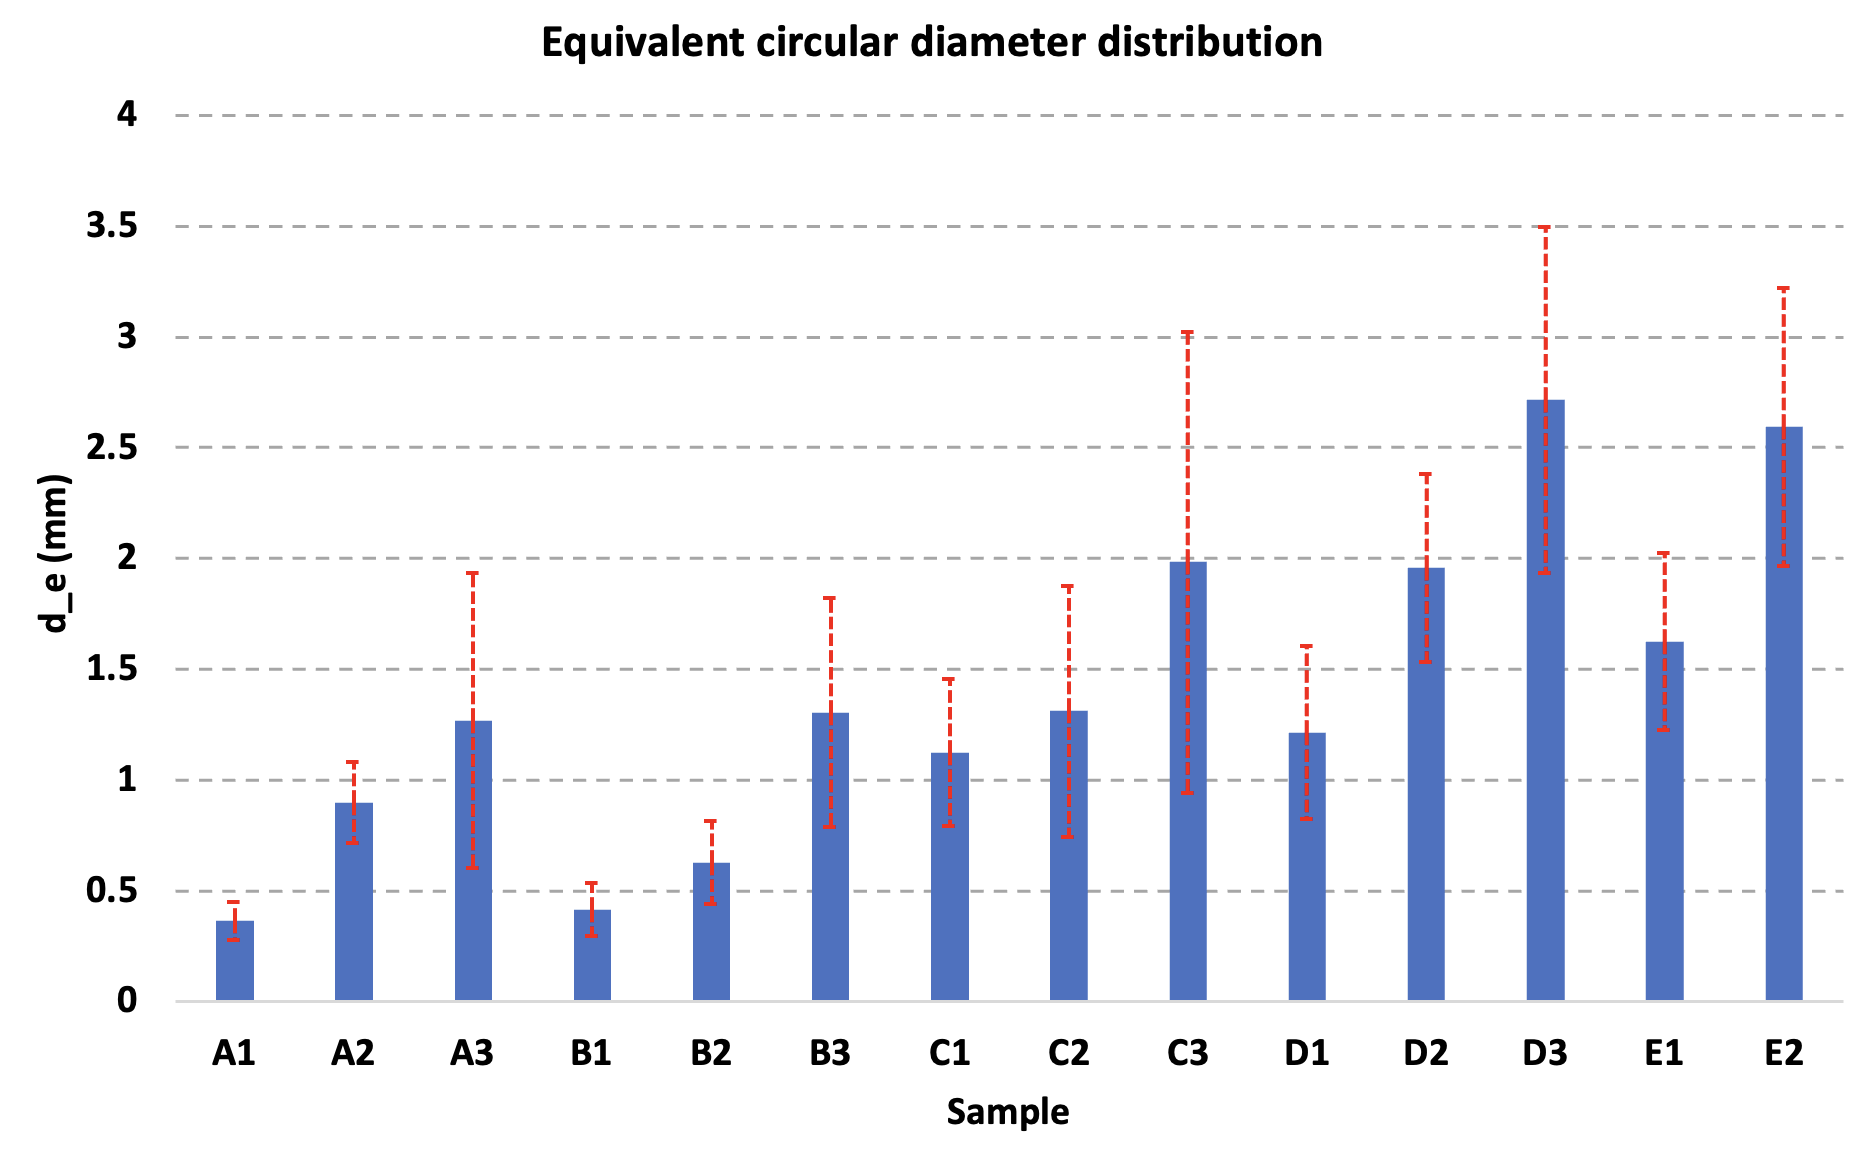
\includegraphics[width=0.95\textwidth]{pory_histogram.png}
    \caption{Histogram of the equivalent circular diameter distribution of the analysed pores.}
    \label{fig:pore_histogram}
\end{figure}

The equivalent circular diameter calculated using Eq.\eqref{eq:equivalent_circular_diameter} describes the two-dimensional size of the visible pore openings in the image plane. Therefore, the method does not provide a direct measurement of the pore volume or the three-dimensional porosity of the material.


\pagebreak
\subsubsection{Porous material samples}
This chapter is focused on the description of the porous material samples used in the experimental research.
Various samples of different materials were investigated by optical microscopy and then tested in the TEALC experimental loop to evaluate their hydraulic performance.
Porosity of samples was measured by helium pycnometry.
Table \ref{tab:vzorky23} shows the list of samples, their material and the measured porosity and average pore size.
Selected materials have different microscopic structure, since they are manufactured by different technologies.
Images of all samples taken by optical microscopy are shown below in Figures \ref{fig:sadavzorku1}, \ref{fig:sadavzorku2} and \ref{fig:sadavzorku3}.

\begin{table}[h!]
\centering
\begin{tabular}{|c|c|c|c|c|}
\hline
\textbf{Sample name} & \textbf{Material} & \textbf{Porosity} & \textbf{Avg. $d_{\mathrm{e}}$} & \textbf{Material $\lambda$} [$\mathrm{W\,m^{-1}\,K^{-1}}$] \\ \hline
A1 & $Cu$ & 96.0 & 0.36 & 395 \\ \hline
A2 & $Cu$ & 97.0 & 0.89 & 395 \\ \hline
A3 & $Cu$ & 96.8 & 1.26 & 395 \\ \hline
B1 & $Sn$ & 91.5 & 0.41 & 65 \\ \hline
B2 & $Sn$ & 89.3 & 0.62 & 65 \\ \hline
B3 & $Sn$ & 91.5 & 1.30 & 65 \\ \hline
C1 & $Al_2O_3$ & 83.6 & 1.12 & 30 \\ \hline
C2 & $Al_2O_3$ & 86.0 & 1.31 & 30 \\ \hline
C3 & $Al_2O_3$ & 85.1 & 1.98 & 30 \\ \hline
D1 & $ZrO_2$ & 86.3 & 1.21 & 3 \\ \hline
D2 & $ZrO_2$ & 87.3 & 1.96 & 3 \\ \hline
D3 & $ZrO_2$ & 89.0 & 2.71 & 3 \\ \hline
E1 & Polyurethane & 96.0 & 1.62 & 0.3 \\ \hline
E2 & Polyurethane & 95.8 & 2.59 & 0.3 \\ \hline
\end{tabular}
\caption{Table of porous material samples.}
\label{tab:vzorky23}
\end{table}

All of the selected samples were manufactured in dimensions 40x40x15 mm, the water flow in experimental setup was passing through the 40x15 mm face, allowing the flow to develop in the 40 mm length of the sample.
\\
\\
Representative optical micrographs of all porous material samples investigated in this study are presented in Figures~\ref{fig:sadavzorku1}--\ref{fig:sadavzorku3}. All images were acquired under identical microscope magnification and illumination conditions, allowing direct qualitative comparison of the internal porous structures. The micrographs provide an overview of the characteristic pore morphology, ligament arrangement and structural homogeneity of the investigated materials prior to the quantitative image analysis described in the following sections. Although several samples exhibit comparable overall porosity, substantial differences in pore size, pore shape, ligament thickness and structural uniformity are clearly visible. These observations indicate that porosity alone is insufficient to fully characterize the geometry of porous materials, highlighting the importance of additional microstructural parameters for understanding their hydraulic behaviour.
\\
\\
The optical micrographs also reveal clear differences between the metallic and ceramic porous structures, reflecting their fundamentally different manufacturing routes. Metallic foams exhibit a relatively smooth and continuous ligament network formed by the sintering of metallic particles, whereas the ceramic foams are characterized by hollow struts and a more open skeletal structure resulting from the replication process, in which a ceramic slurry is deposited onto a polyurethane template that is subsequently removed during firing. The final group of samples, designated by the letter ``E'', corresponds to the original polyurethane templates supplied by the manufacturer together with the ceramic foams. These templates illustrate the precursor structure used during the manufacturing process and provide a direct comparison between the initial polymer scaffold and the resulting ceramic porous material.

\pagebreak
\begin{figure}[H]
\centering

\begin{subfigure}{0.45\textwidth}
\centering
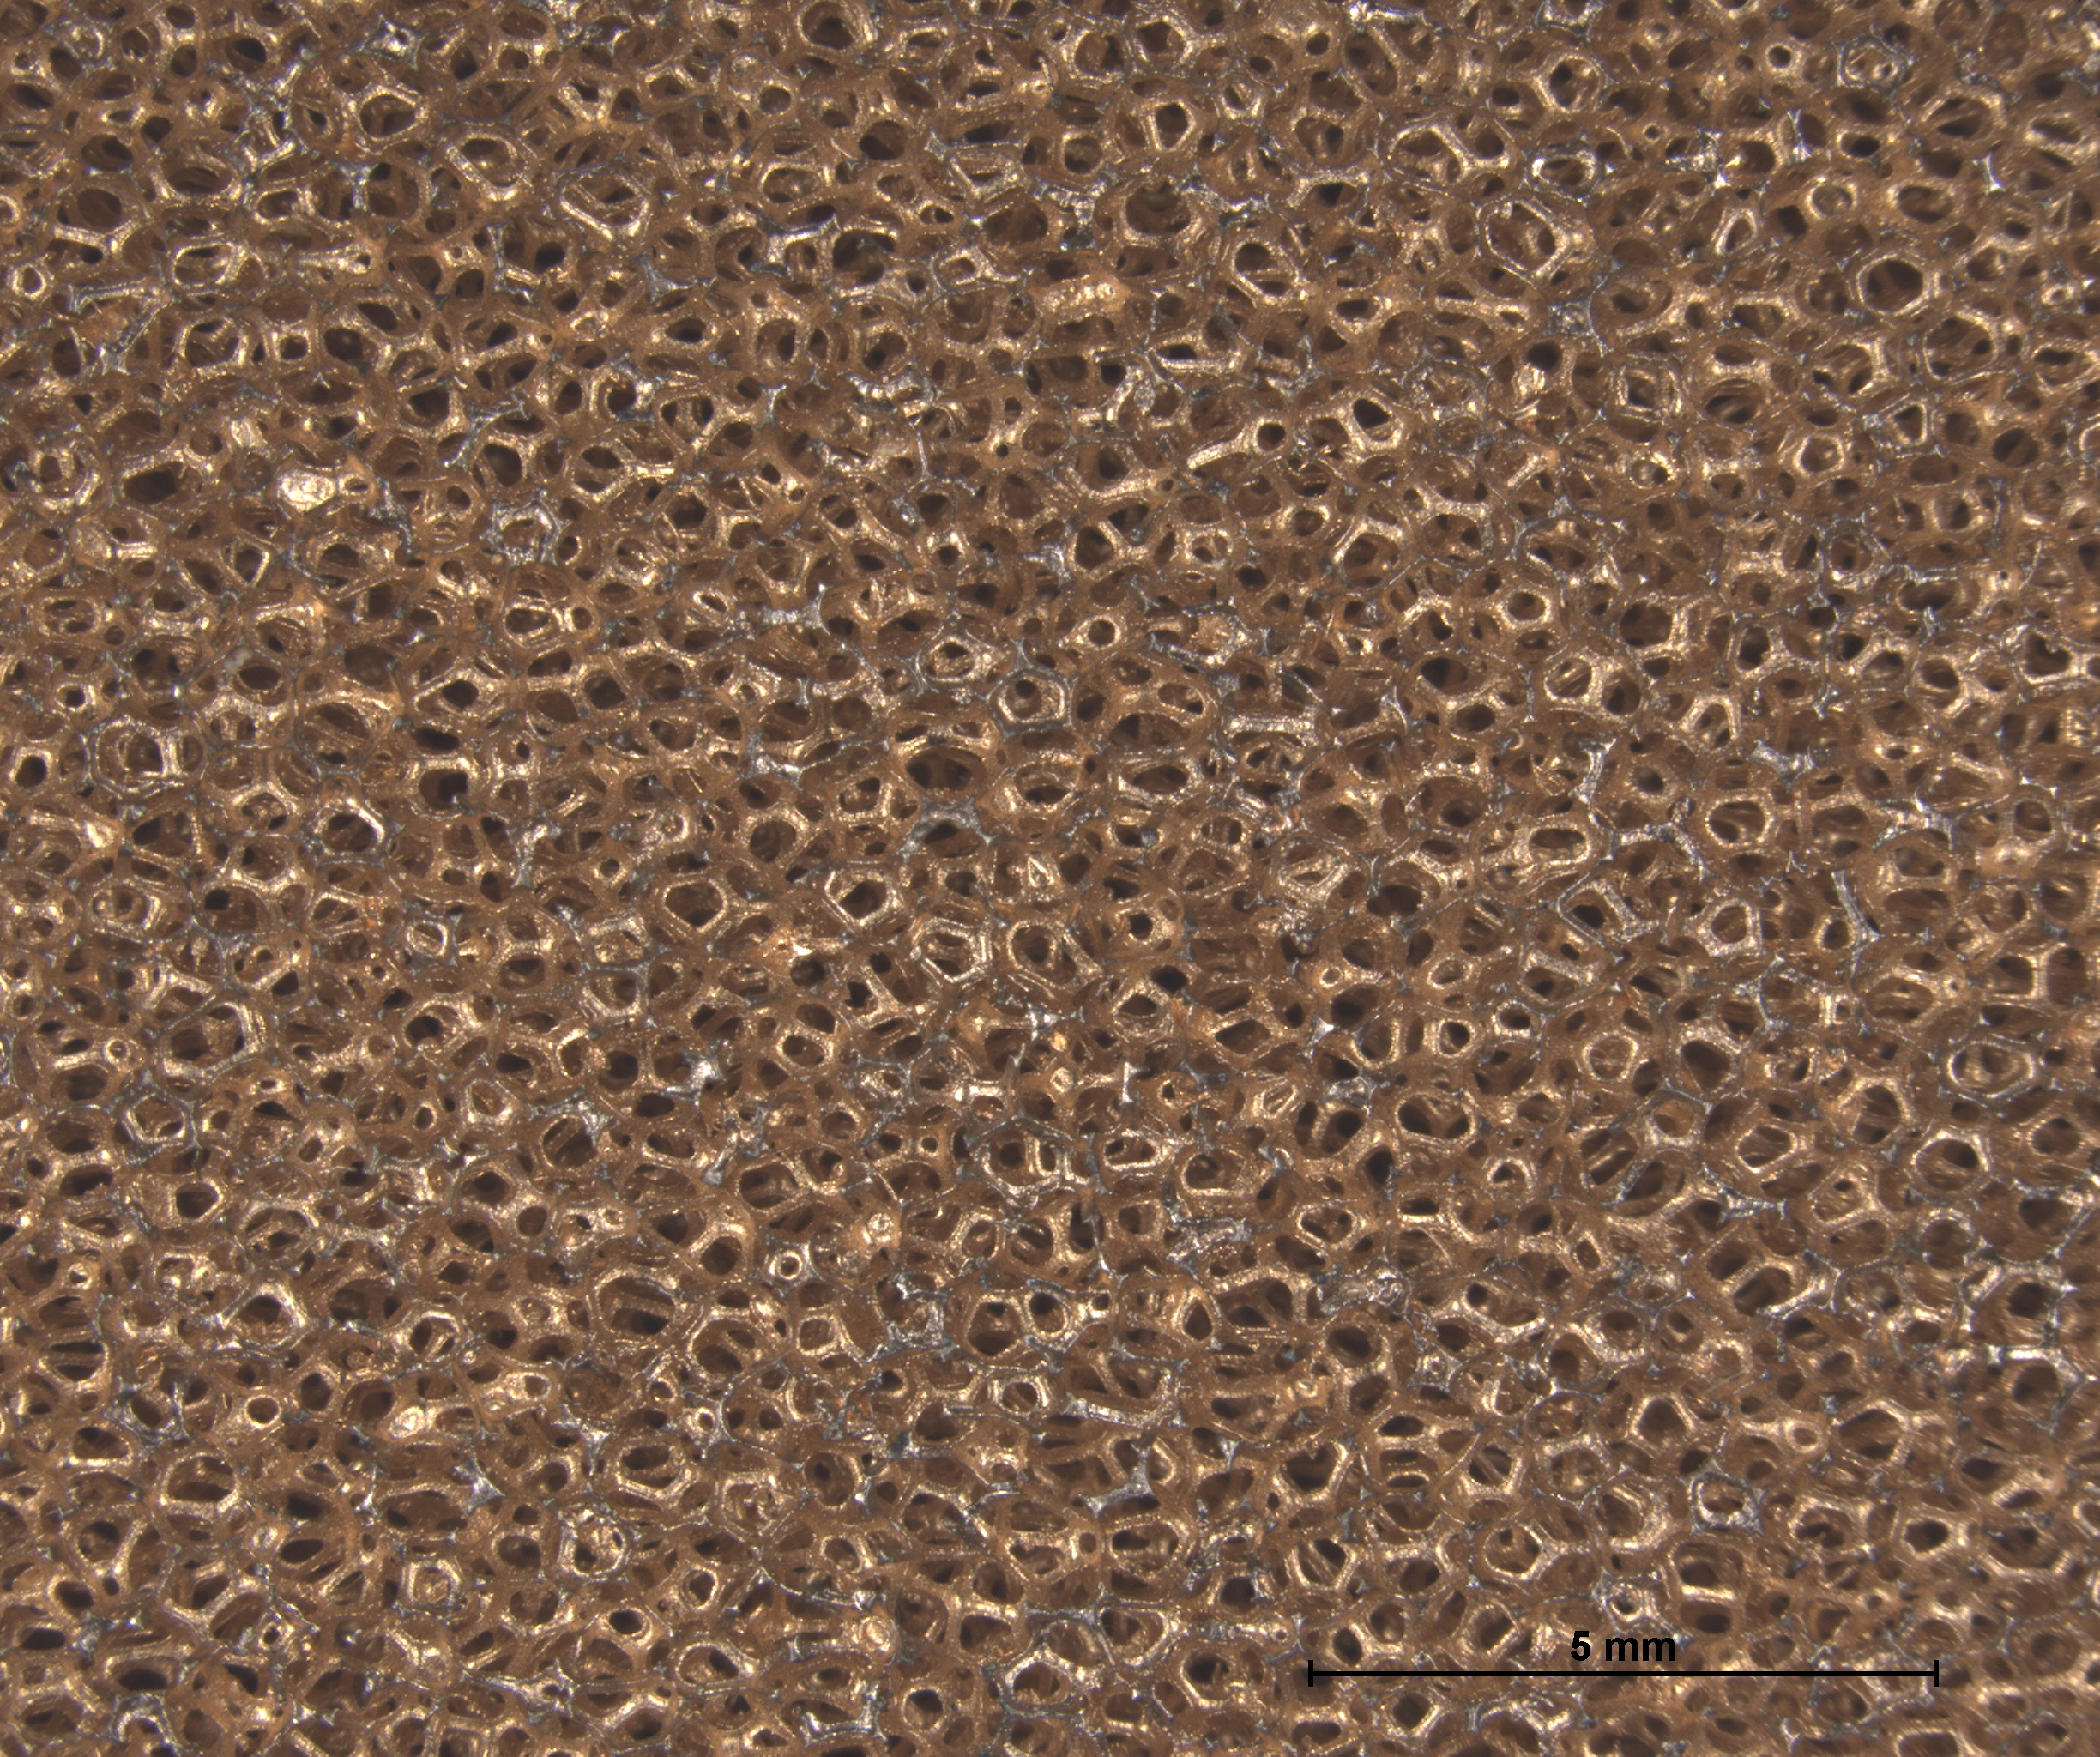
\includegraphics[width=\linewidth]{A1.jpg}
\caption{Sample A1}
\end{subfigure}
\hfill
\begin{subfigure}{0.45\textwidth}
\centering
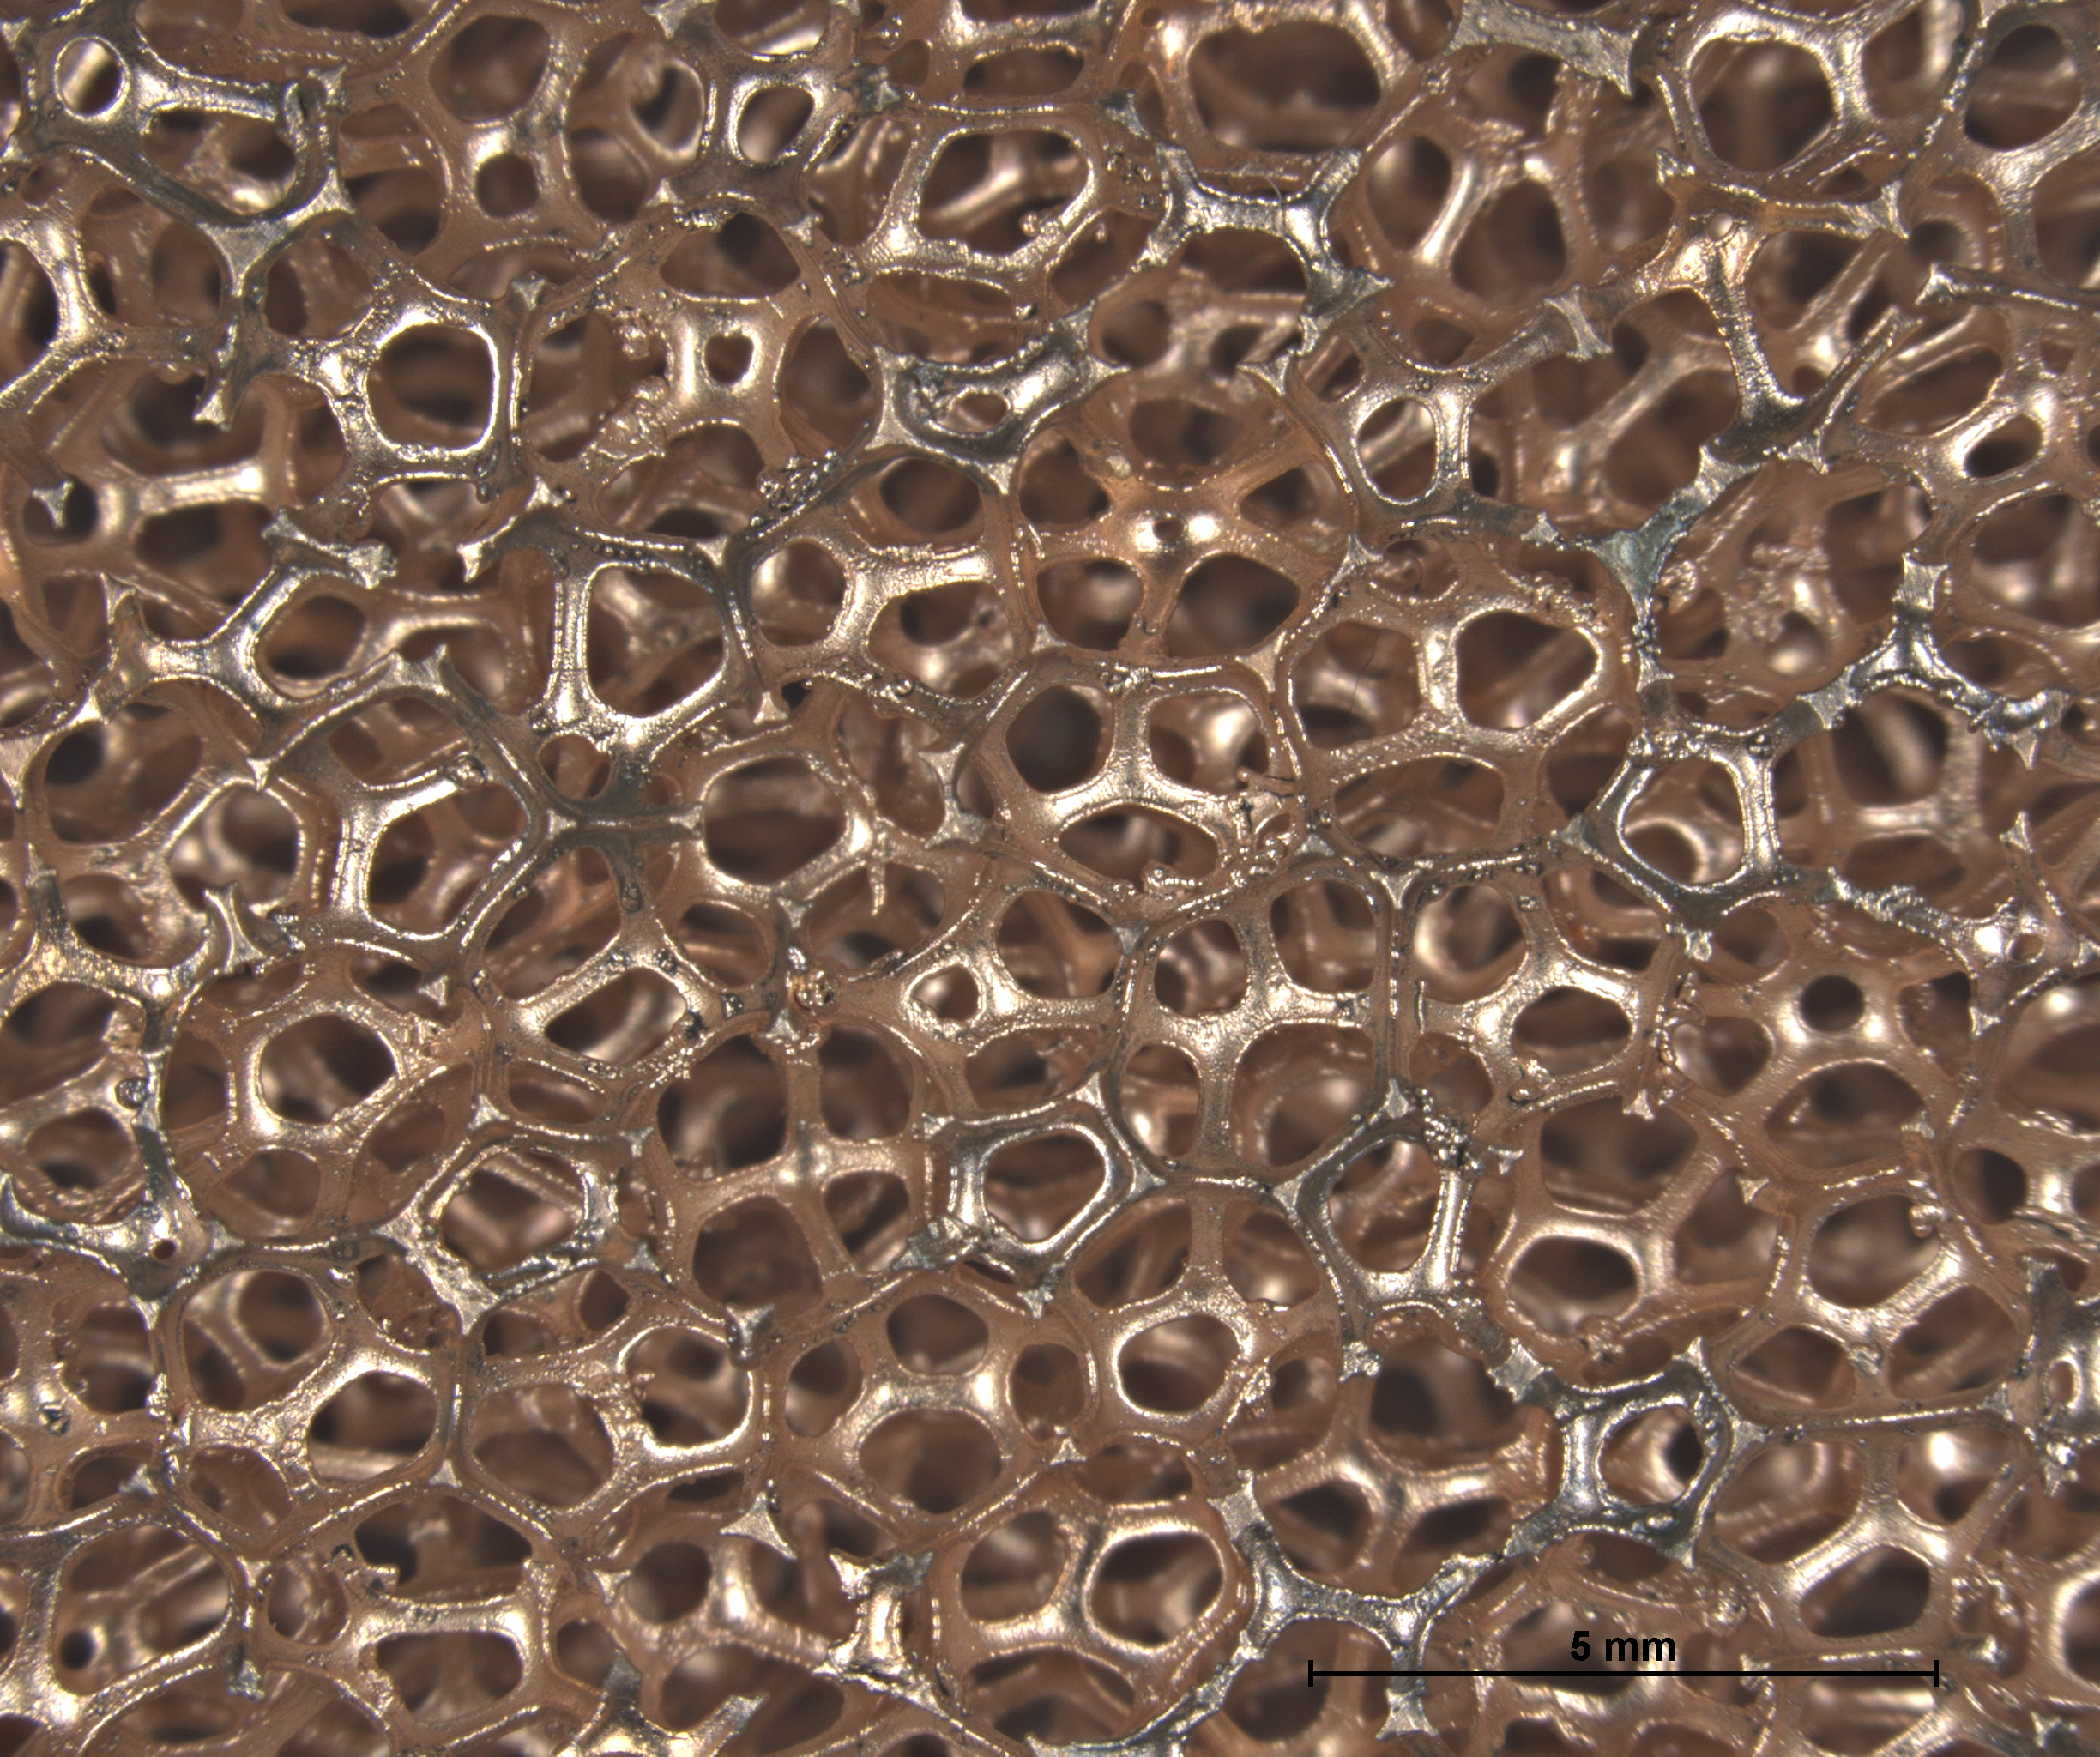
\includegraphics[width=\linewidth]{A2.jpg}
\caption{Sample A2}
\end{subfigure}

\vspace{0.4cm}

\begin{subfigure}{0.45\textwidth}
\centering
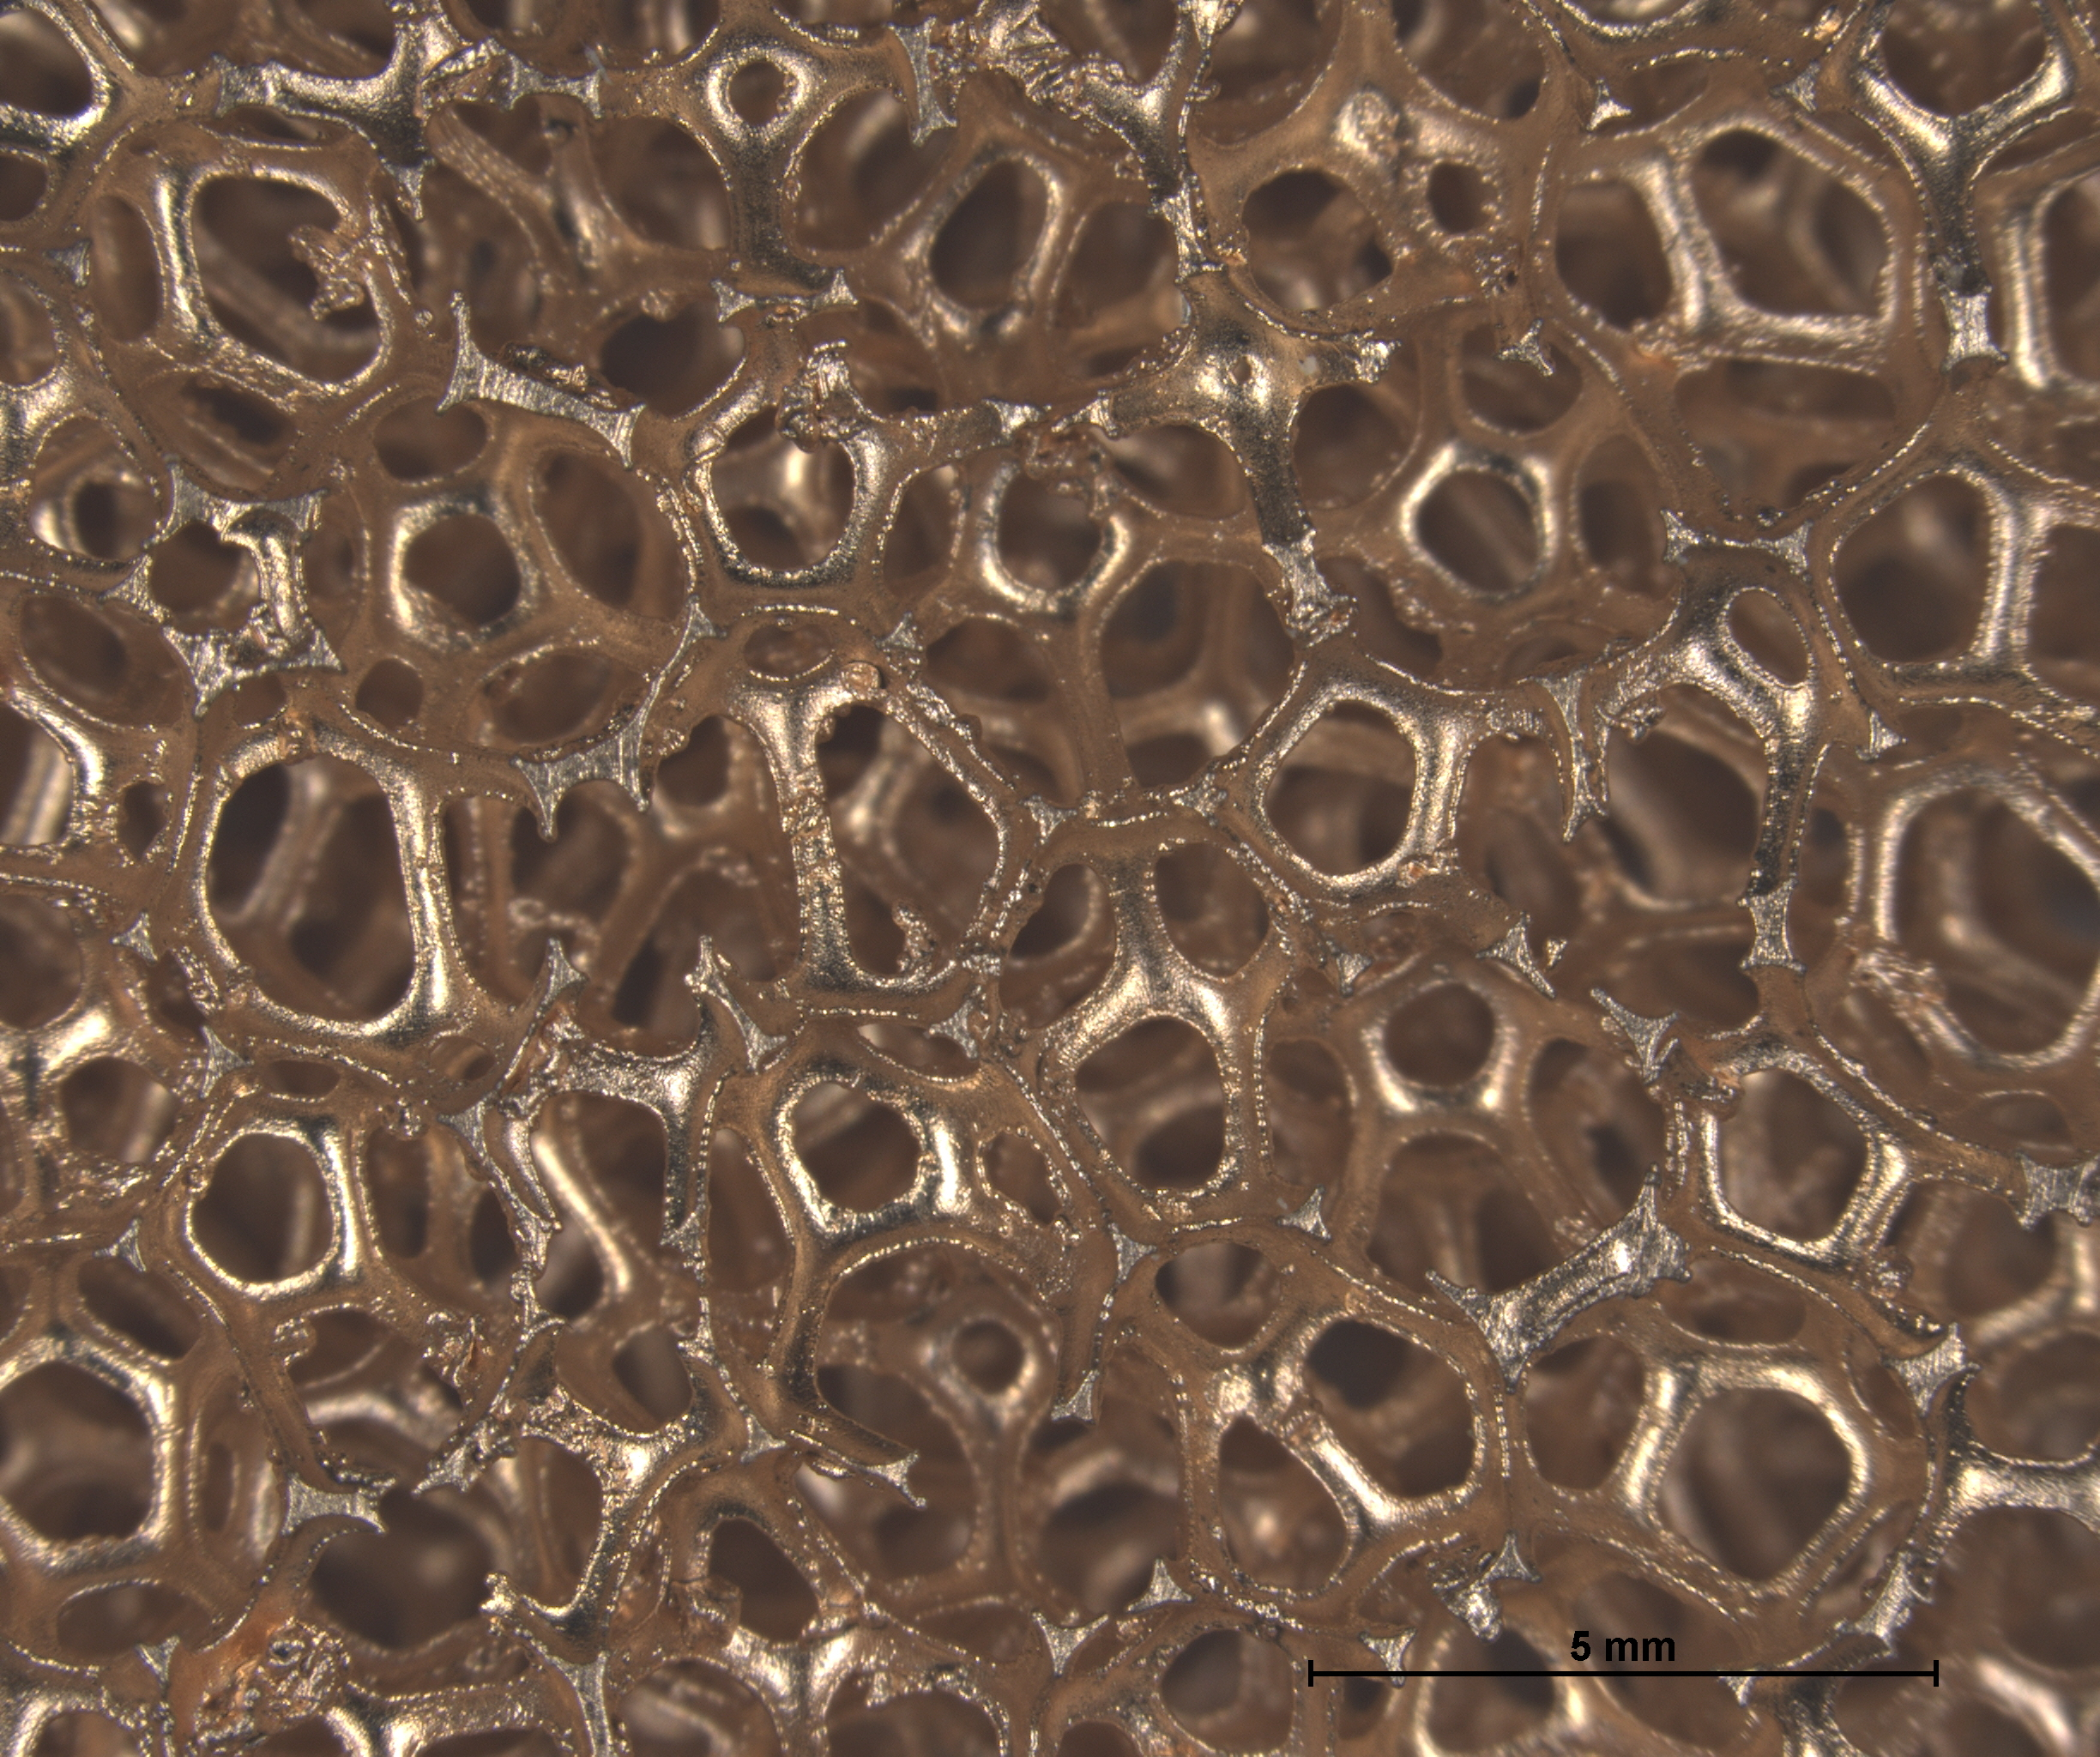
\includegraphics[width=\linewidth]{A3.jpg}
\caption{Sample A3}
\end{subfigure}
\hfill
\begin{subfigure}{0.45\textwidth}
\centering
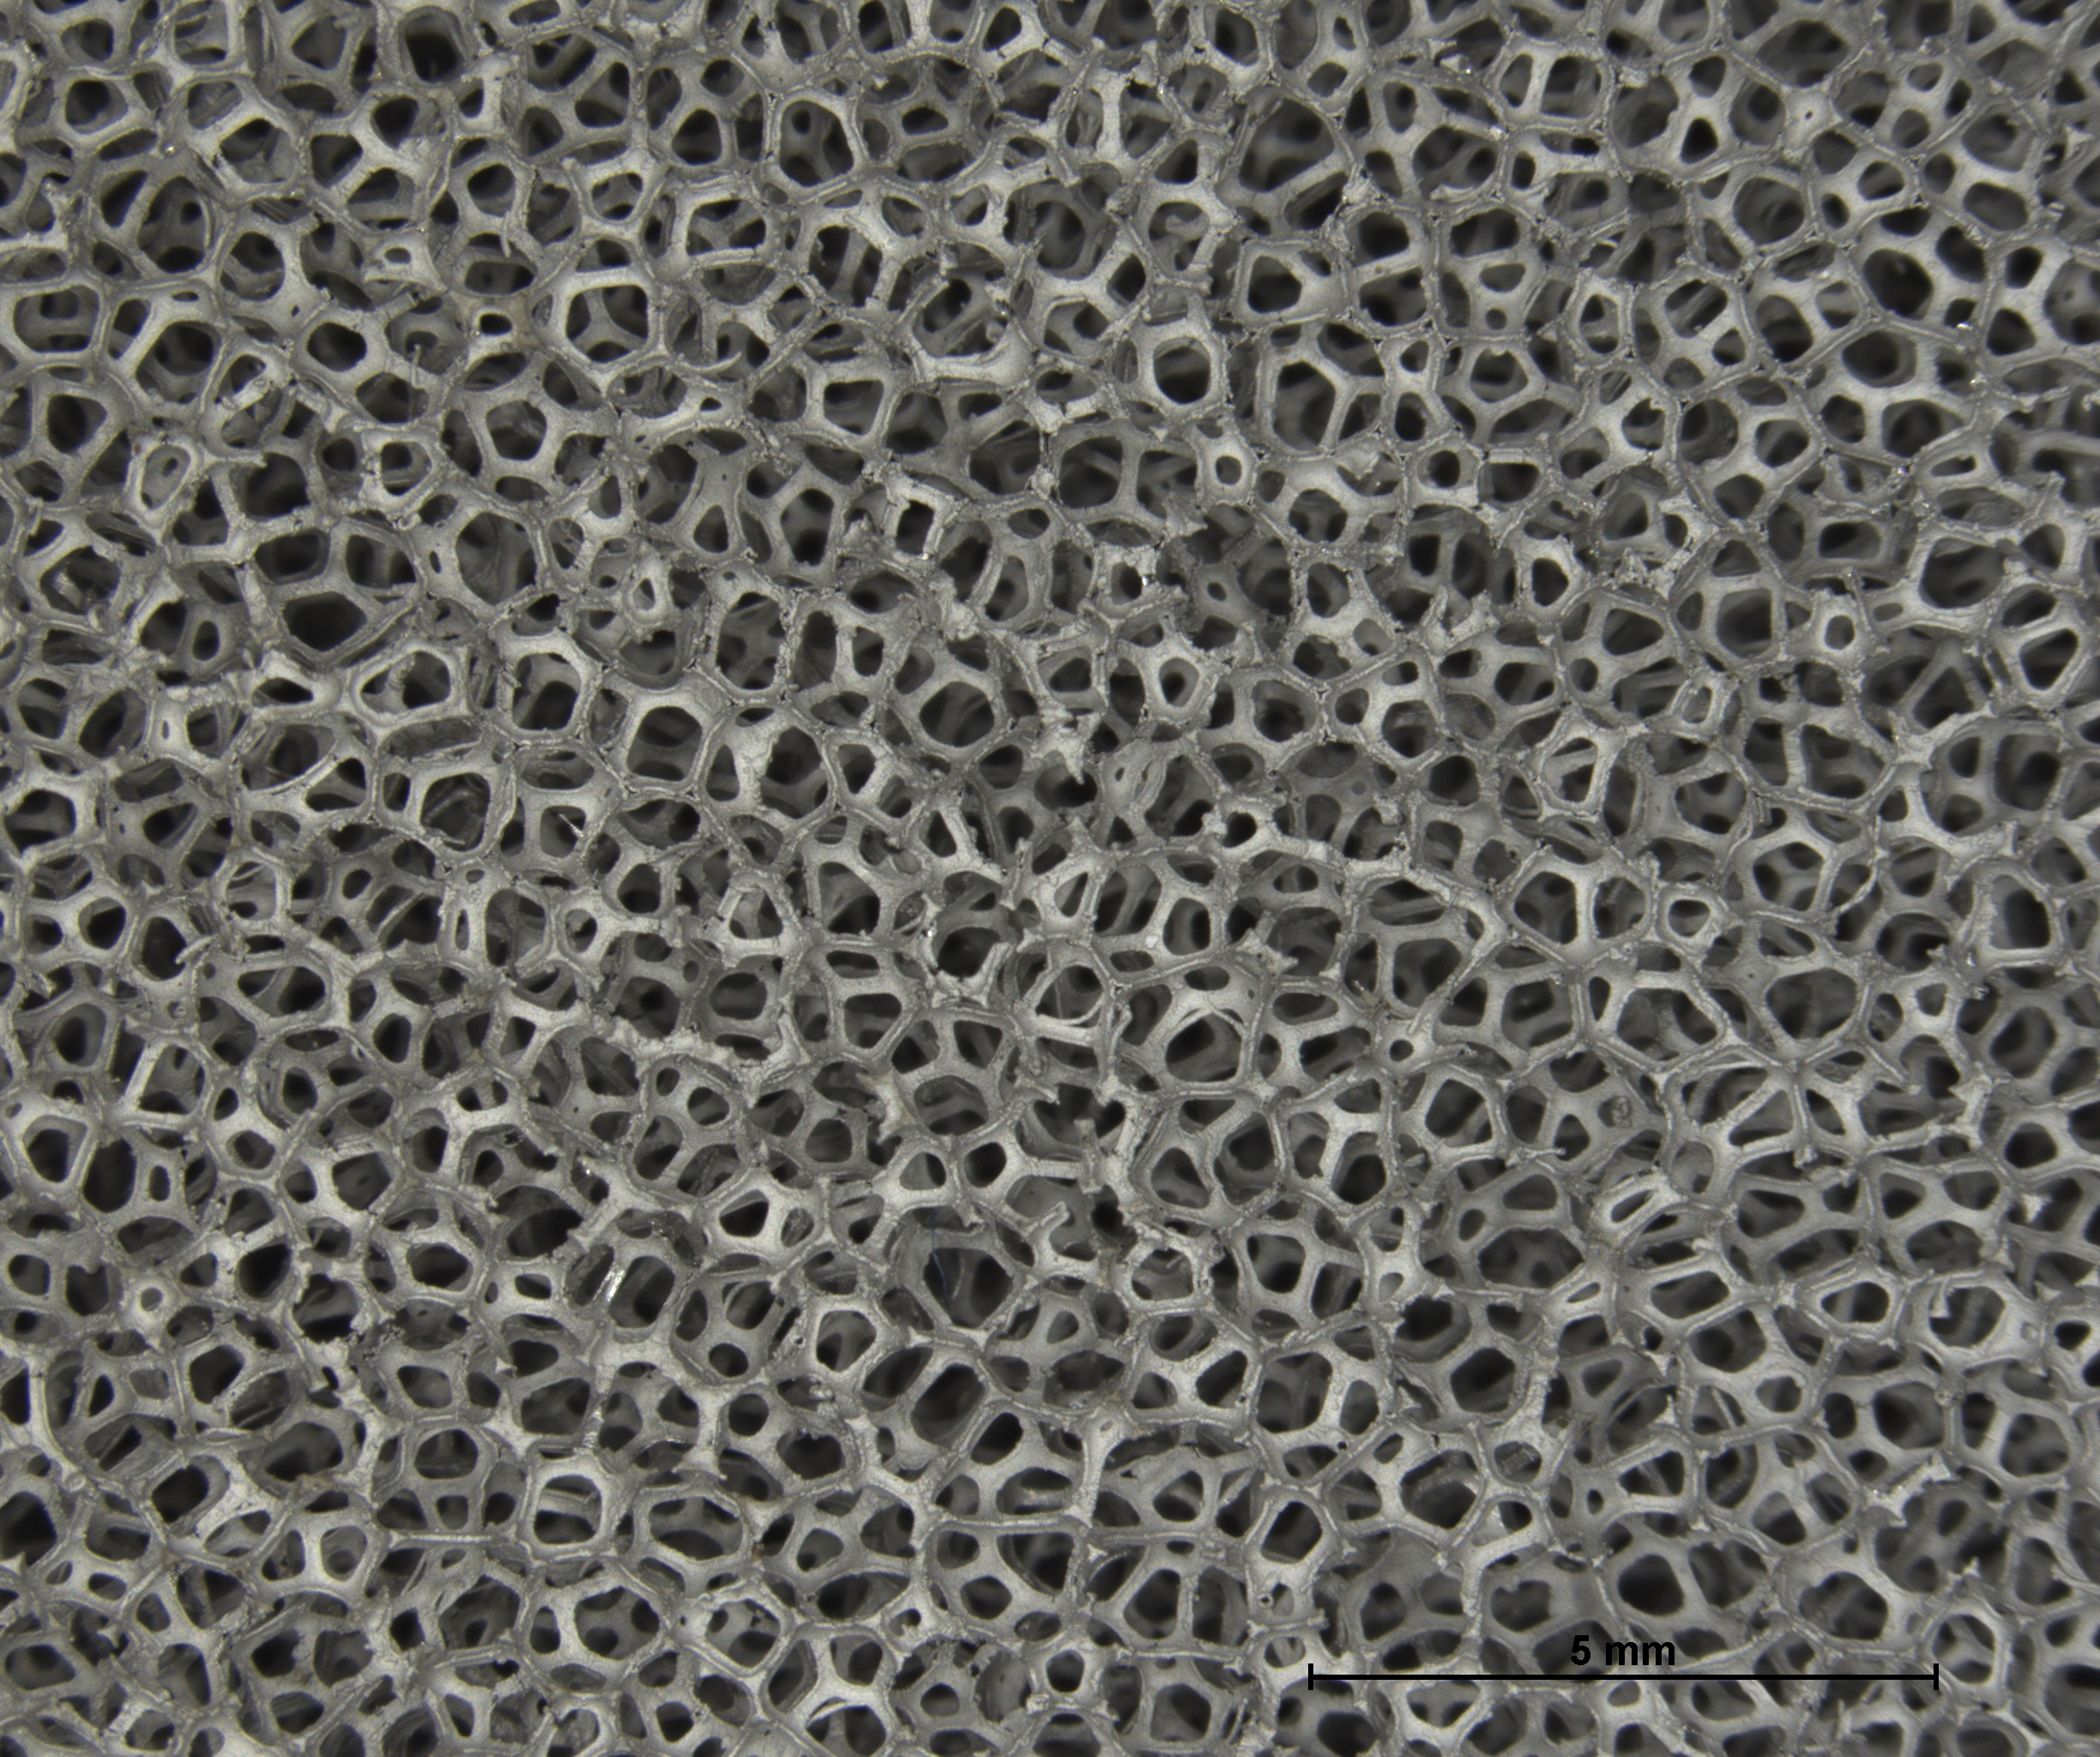
\includegraphics[width=\linewidth]{B1.jpg}
\caption{Sample B1}
\end{subfigure}

\vspace{0.4cm}

\begin{subfigure}{0.45\textwidth}
\centering
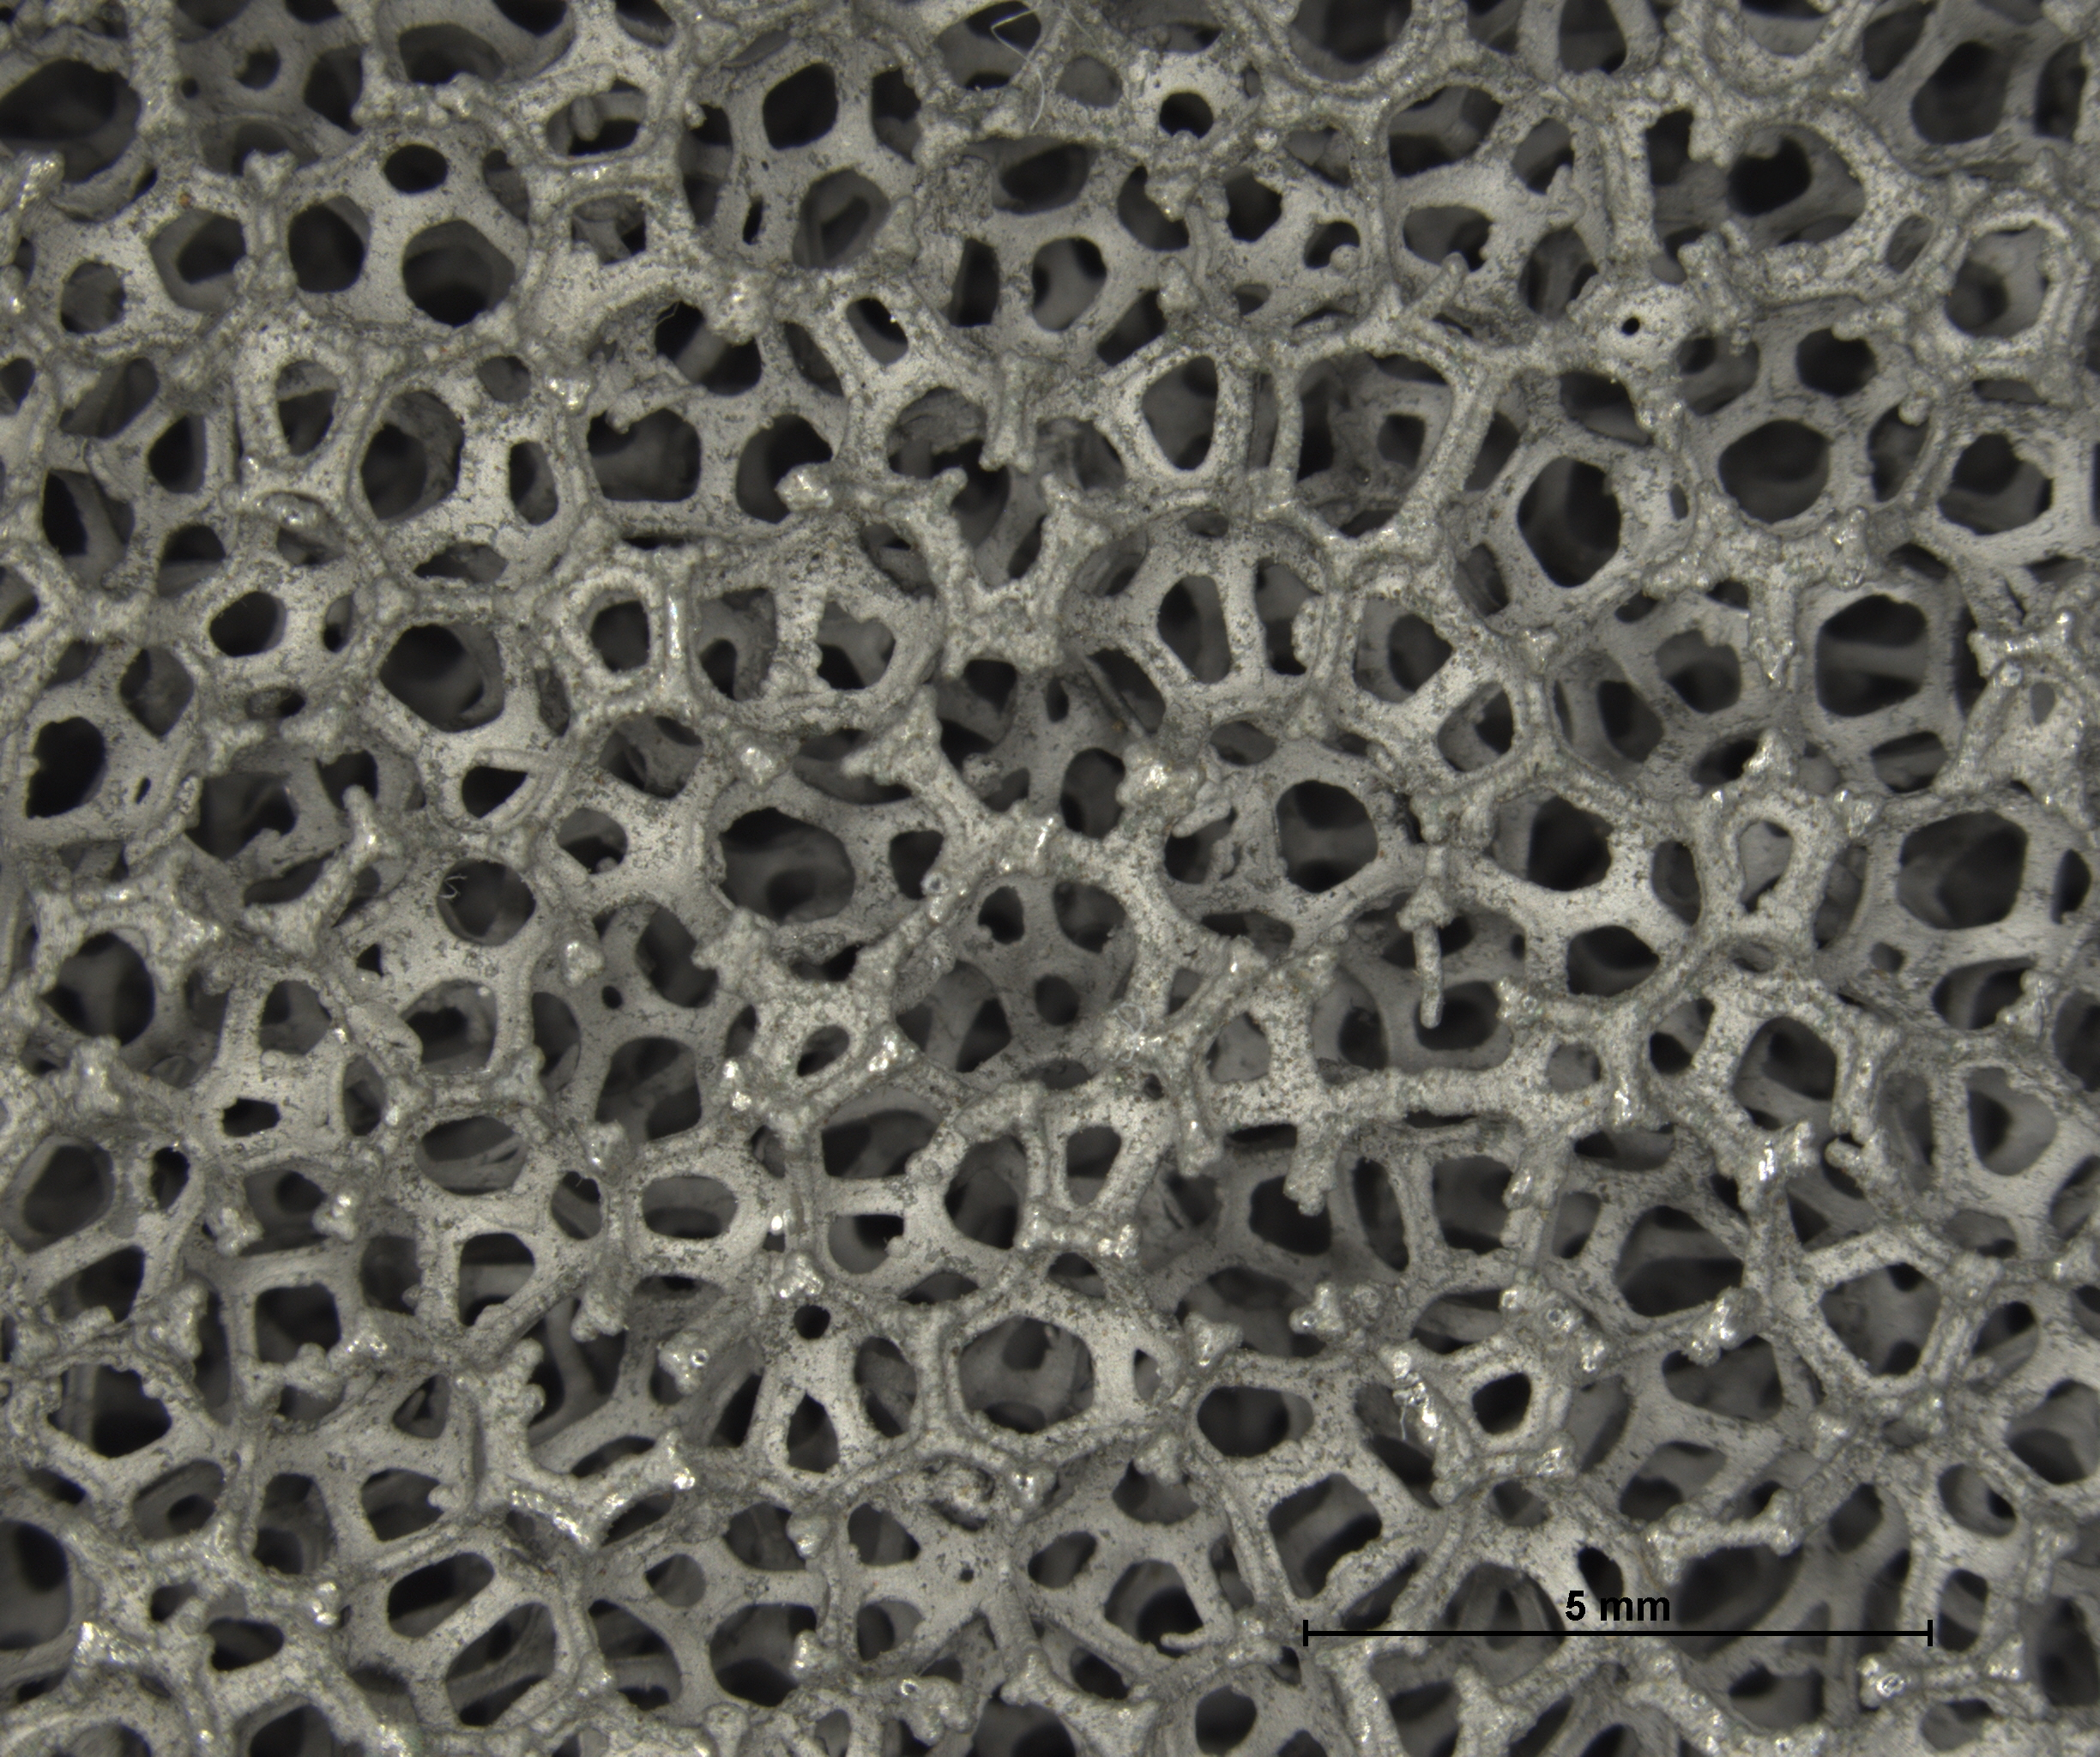
\includegraphics[width=\linewidth]{B2.jpg}
\caption{Sample B2}
\end{subfigure}
\hfill
\begin{subfigure}{0.45\textwidth}
\centering
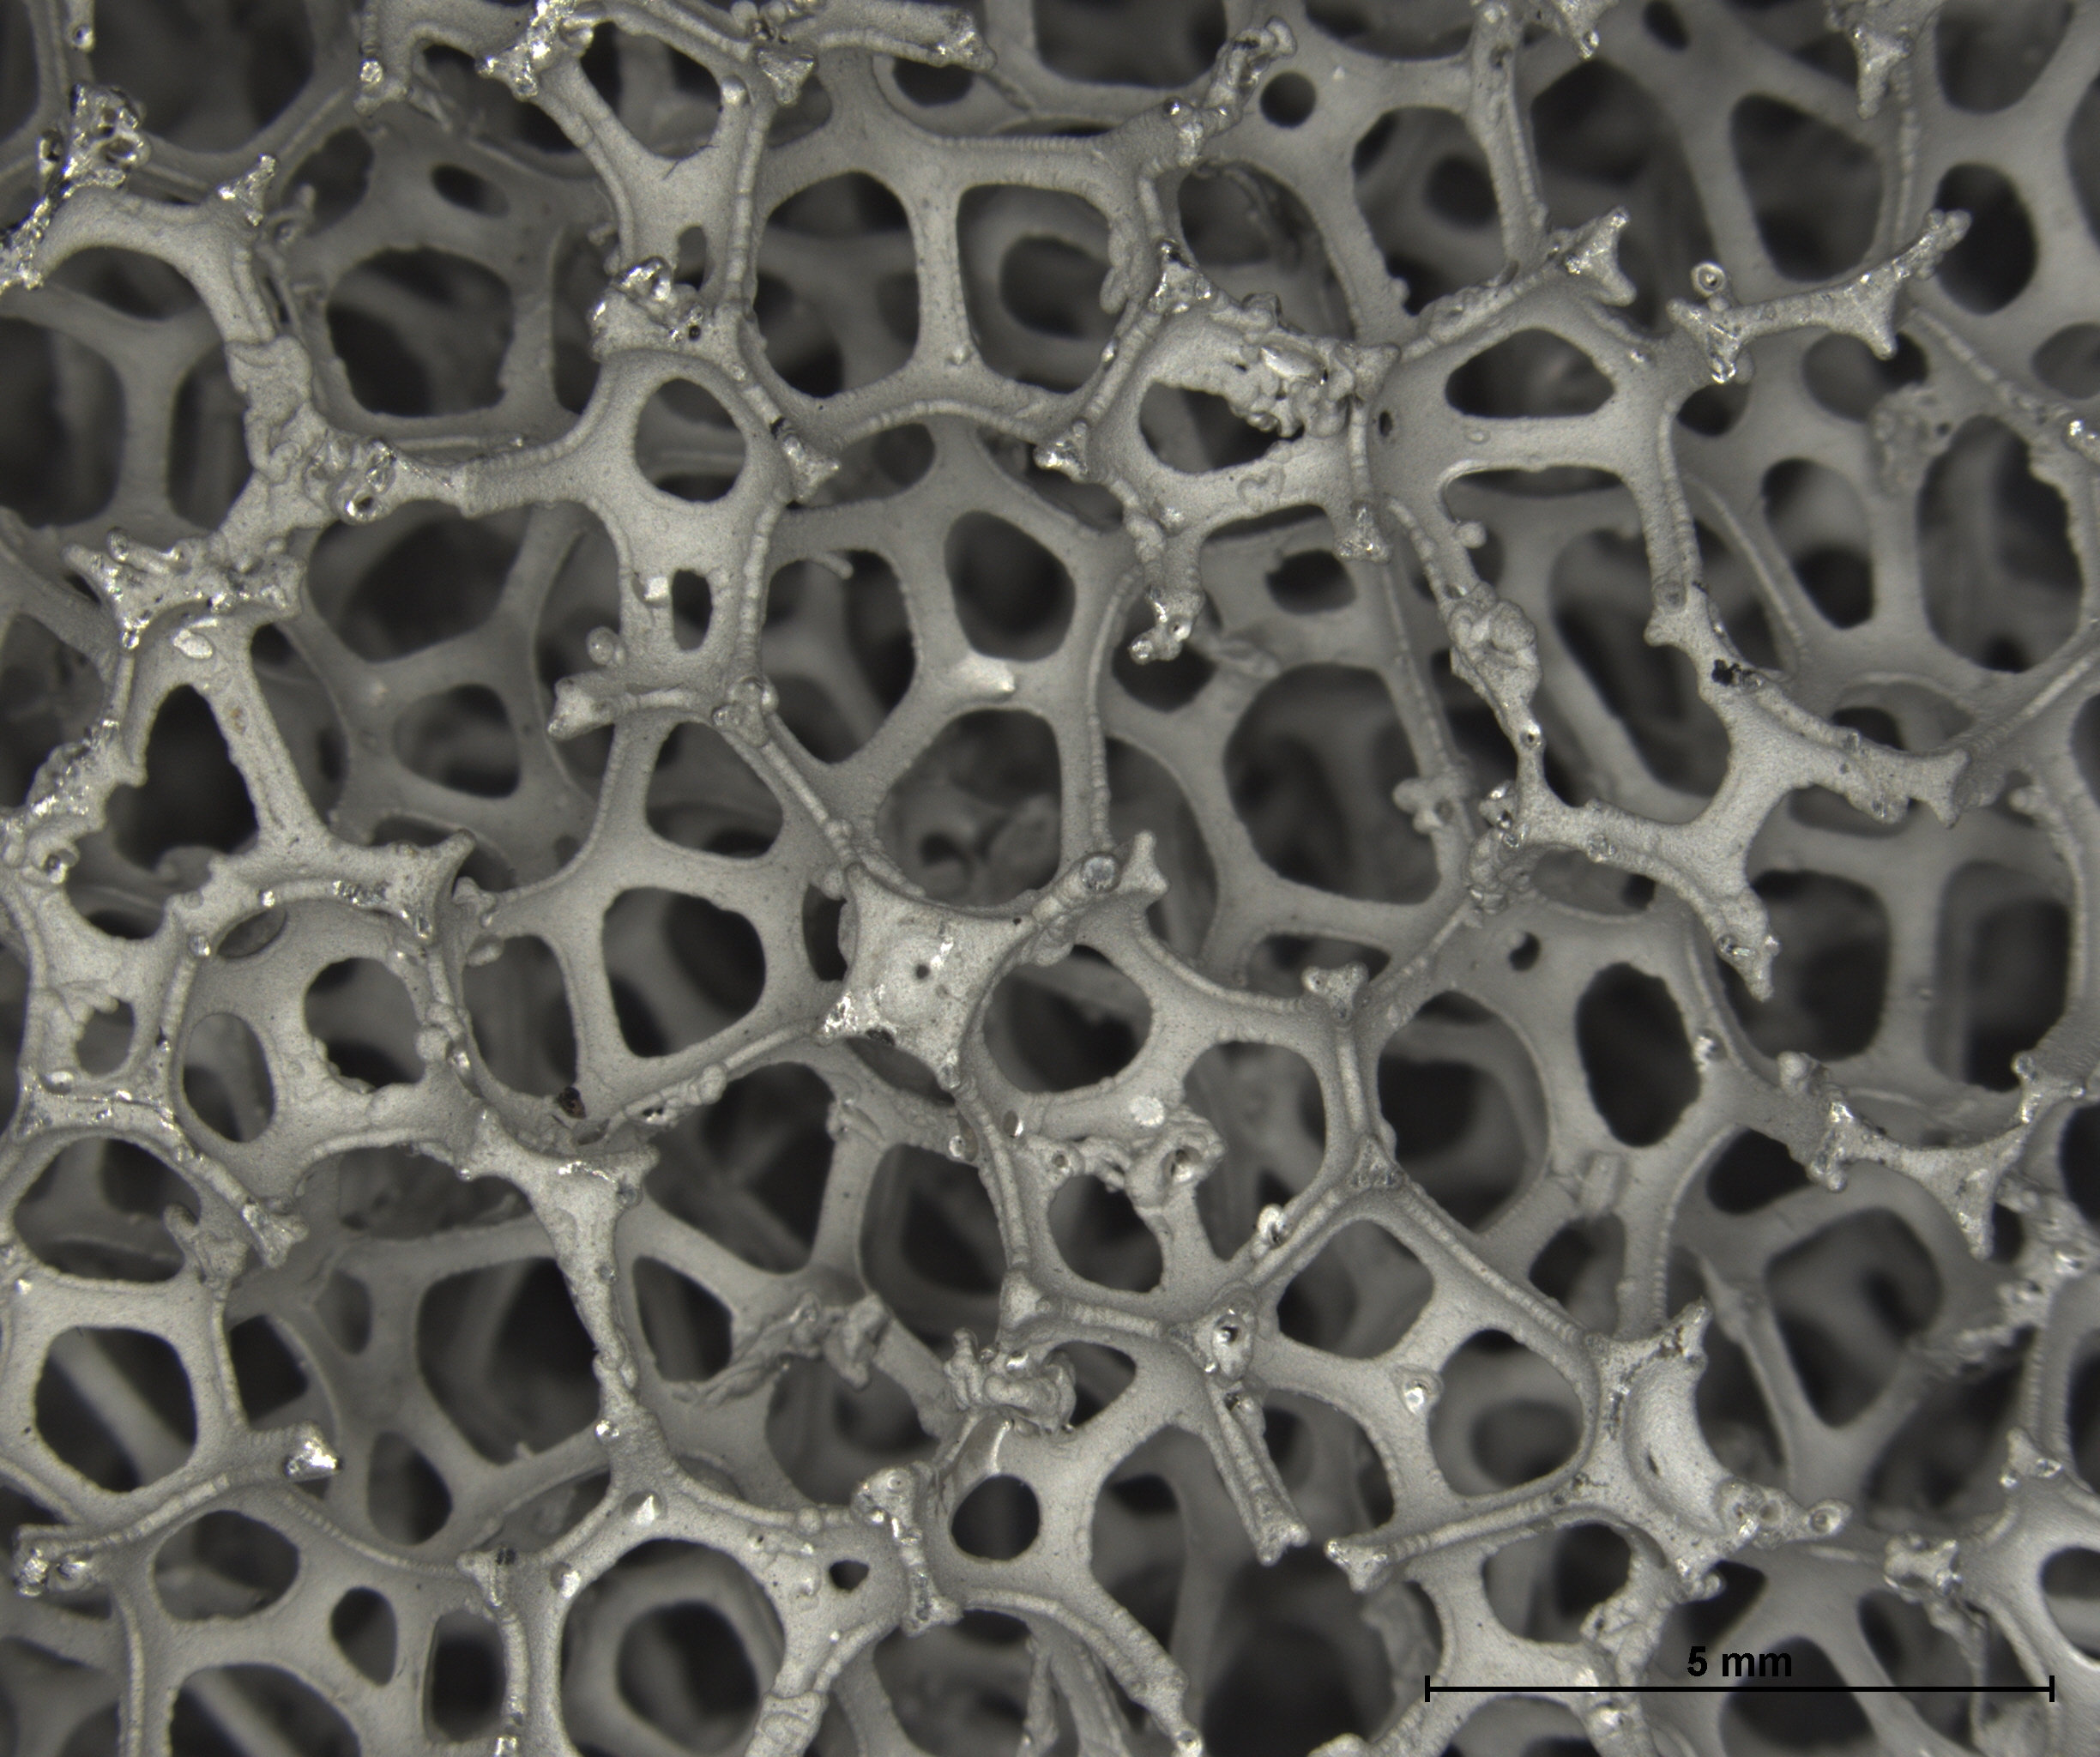
\includegraphics[width=\linewidth]{B3.jpg}
\caption{Sample B3}
\end{subfigure}

\caption{Porous material samples - Set 1}
\label{fig:sadavzorku1}
\end{figure}

\pagebreak

\begin{figure}[H]
\centering

\begin{subfigure}{0.45\textwidth}
\centering
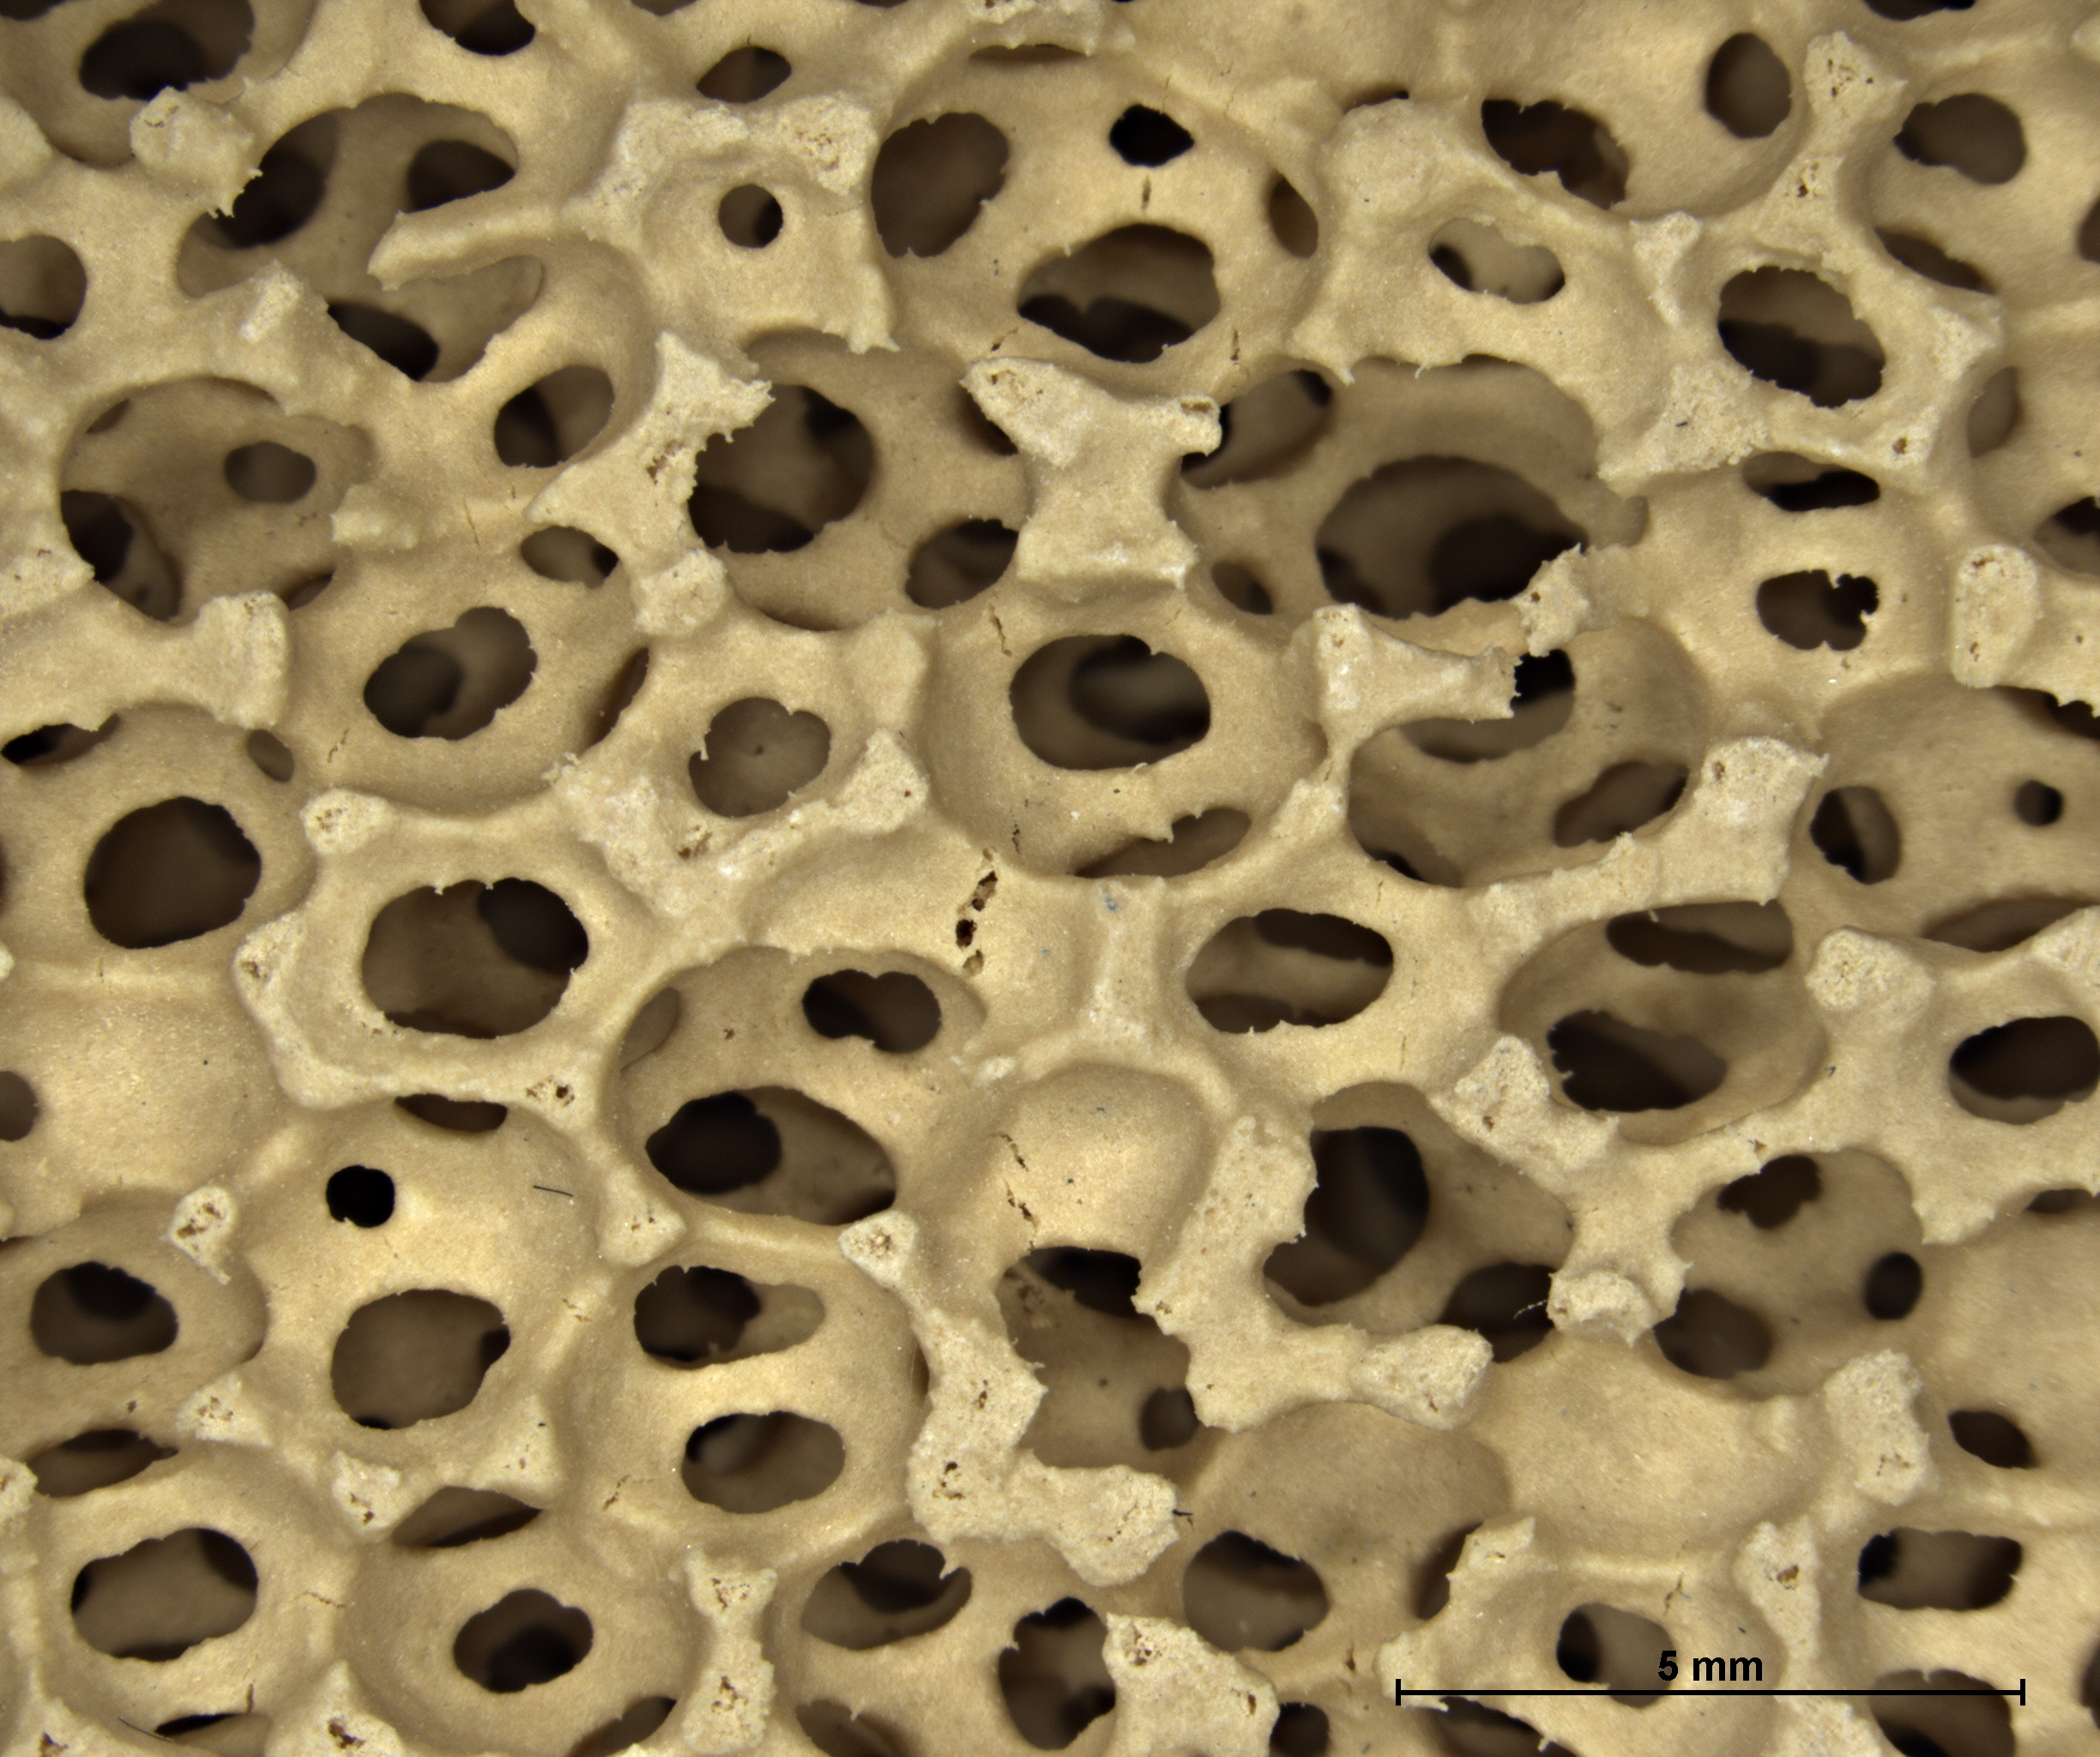
\includegraphics[width=\linewidth]{C1.jpg}
\caption{Sample C1}
\end{subfigure}
\hfill
\begin{subfigure}{0.45\textwidth}
\centering
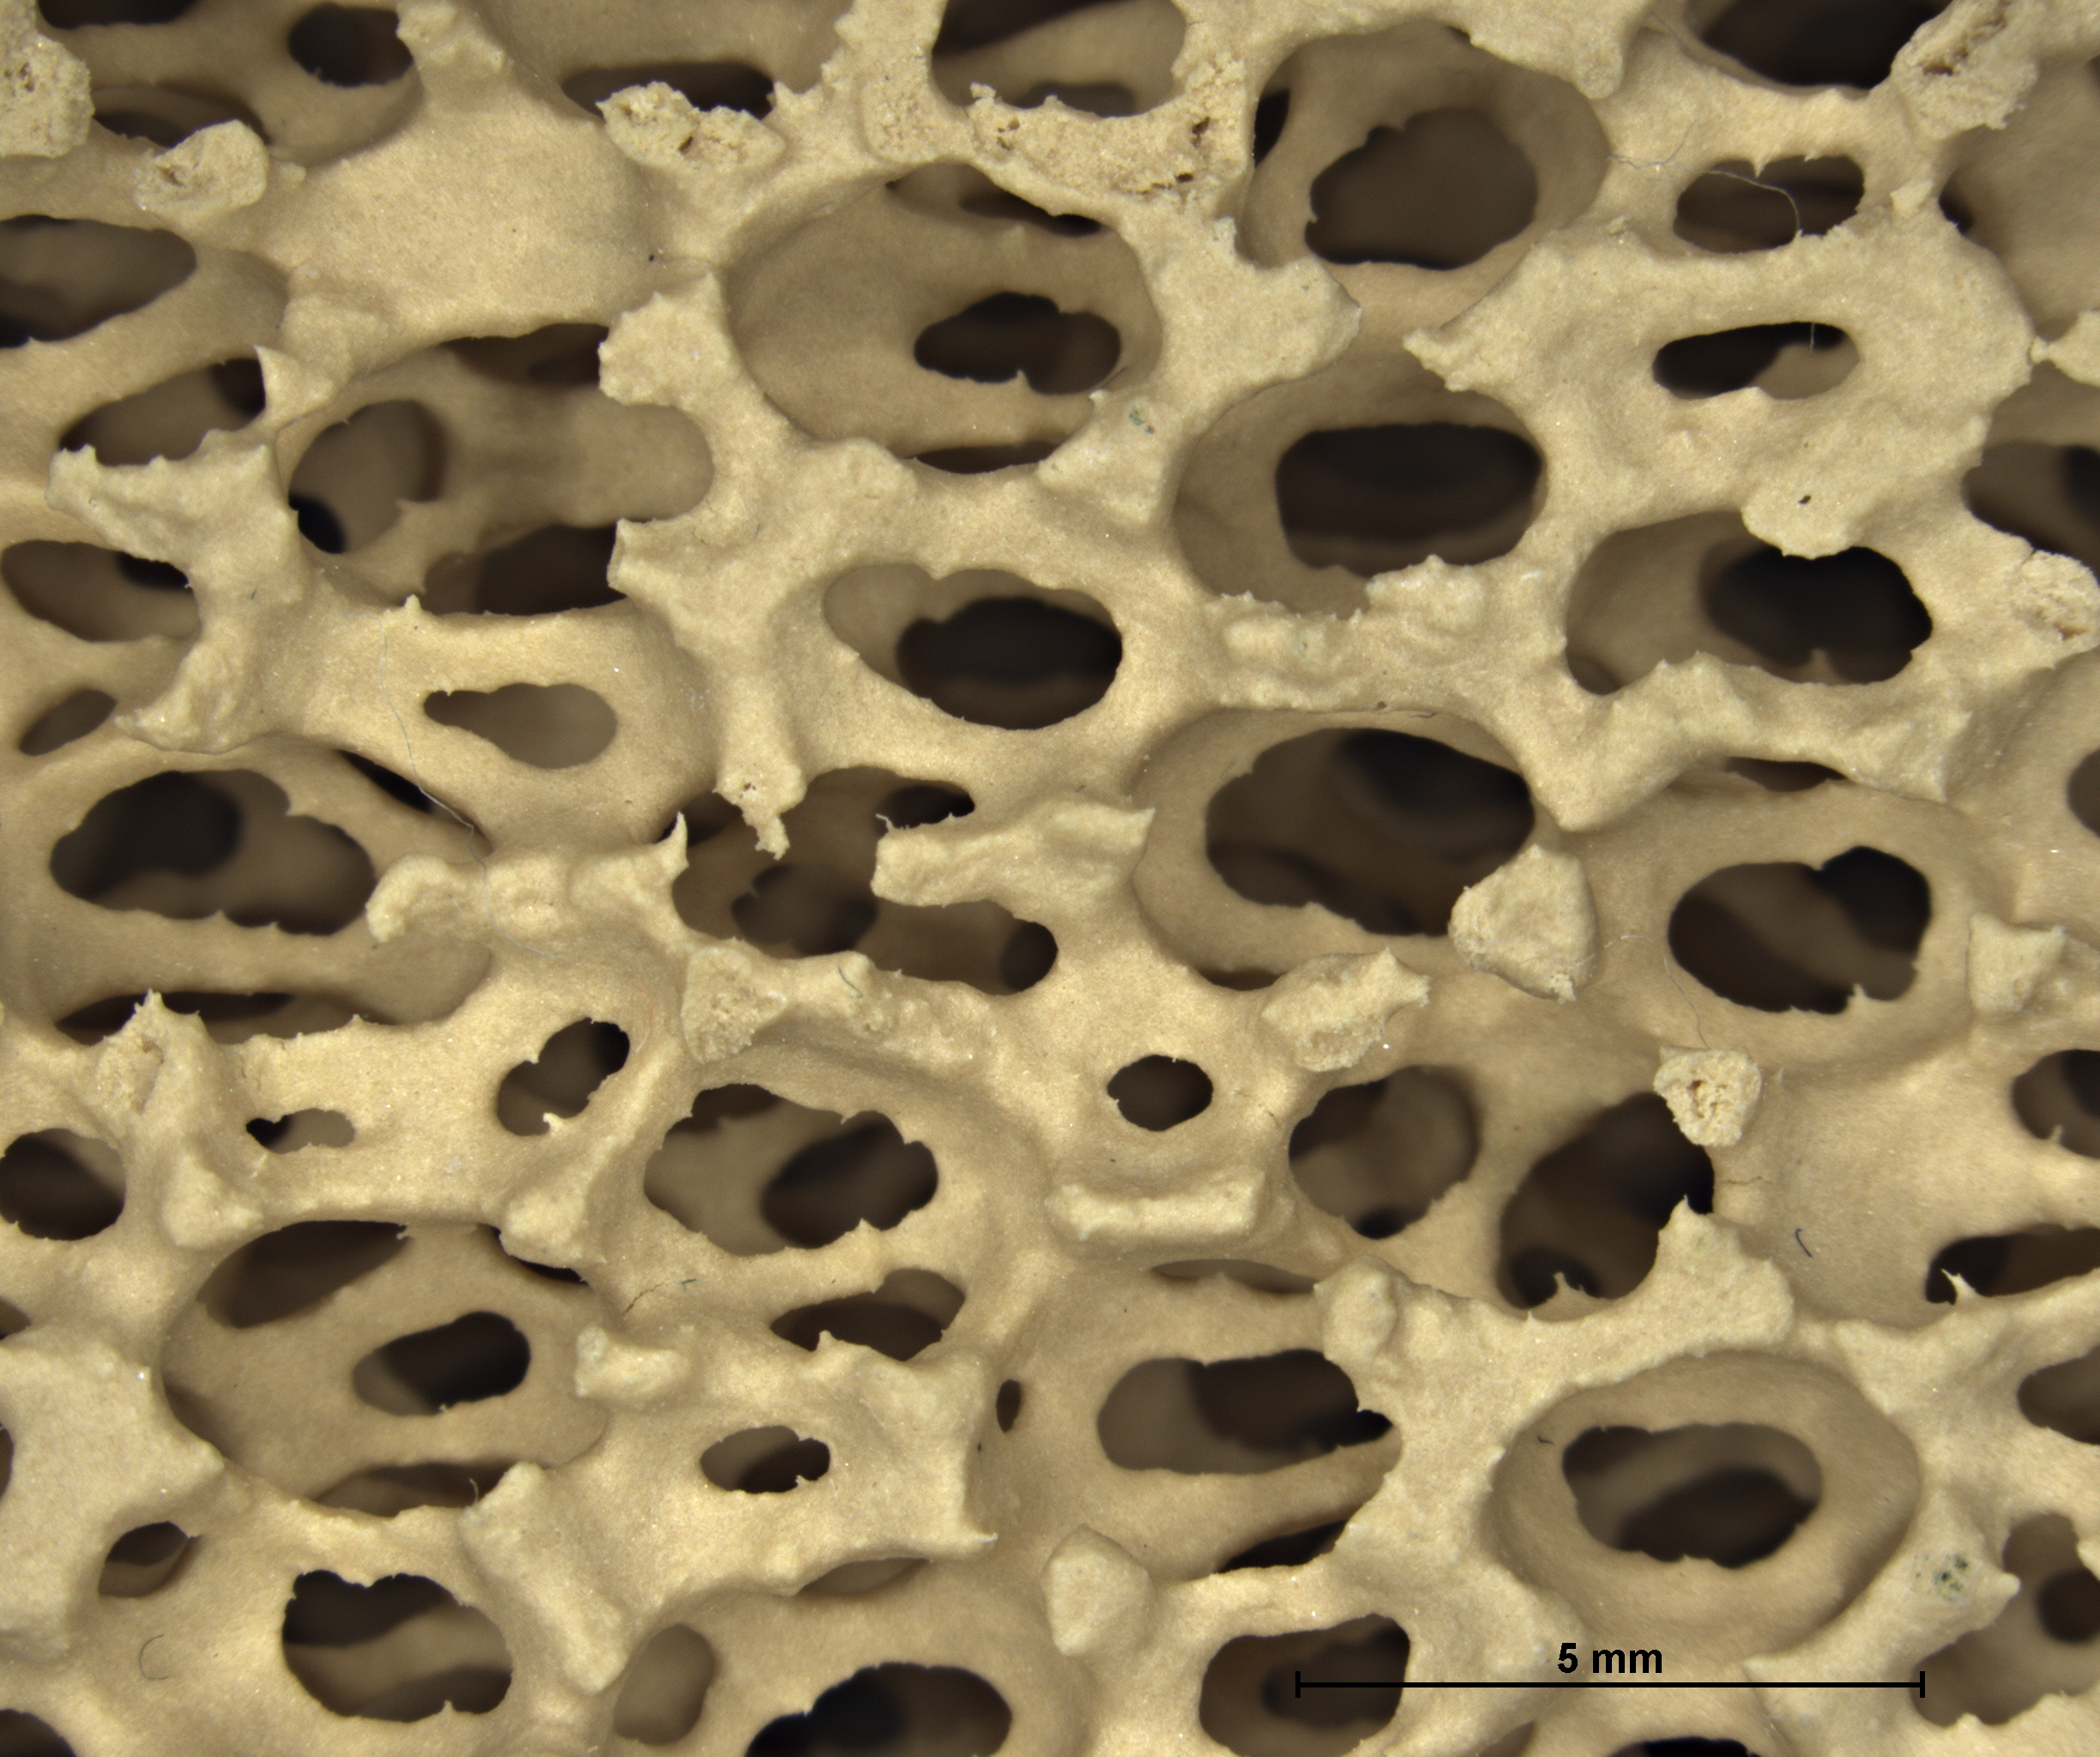
\includegraphics[width=\linewidth]{C2.jpg}
\caption{Sample C2}
\end{subfigure}

\vspace{0.4cm}

\begin{subfigure}{0.45\textwidth}
\centering
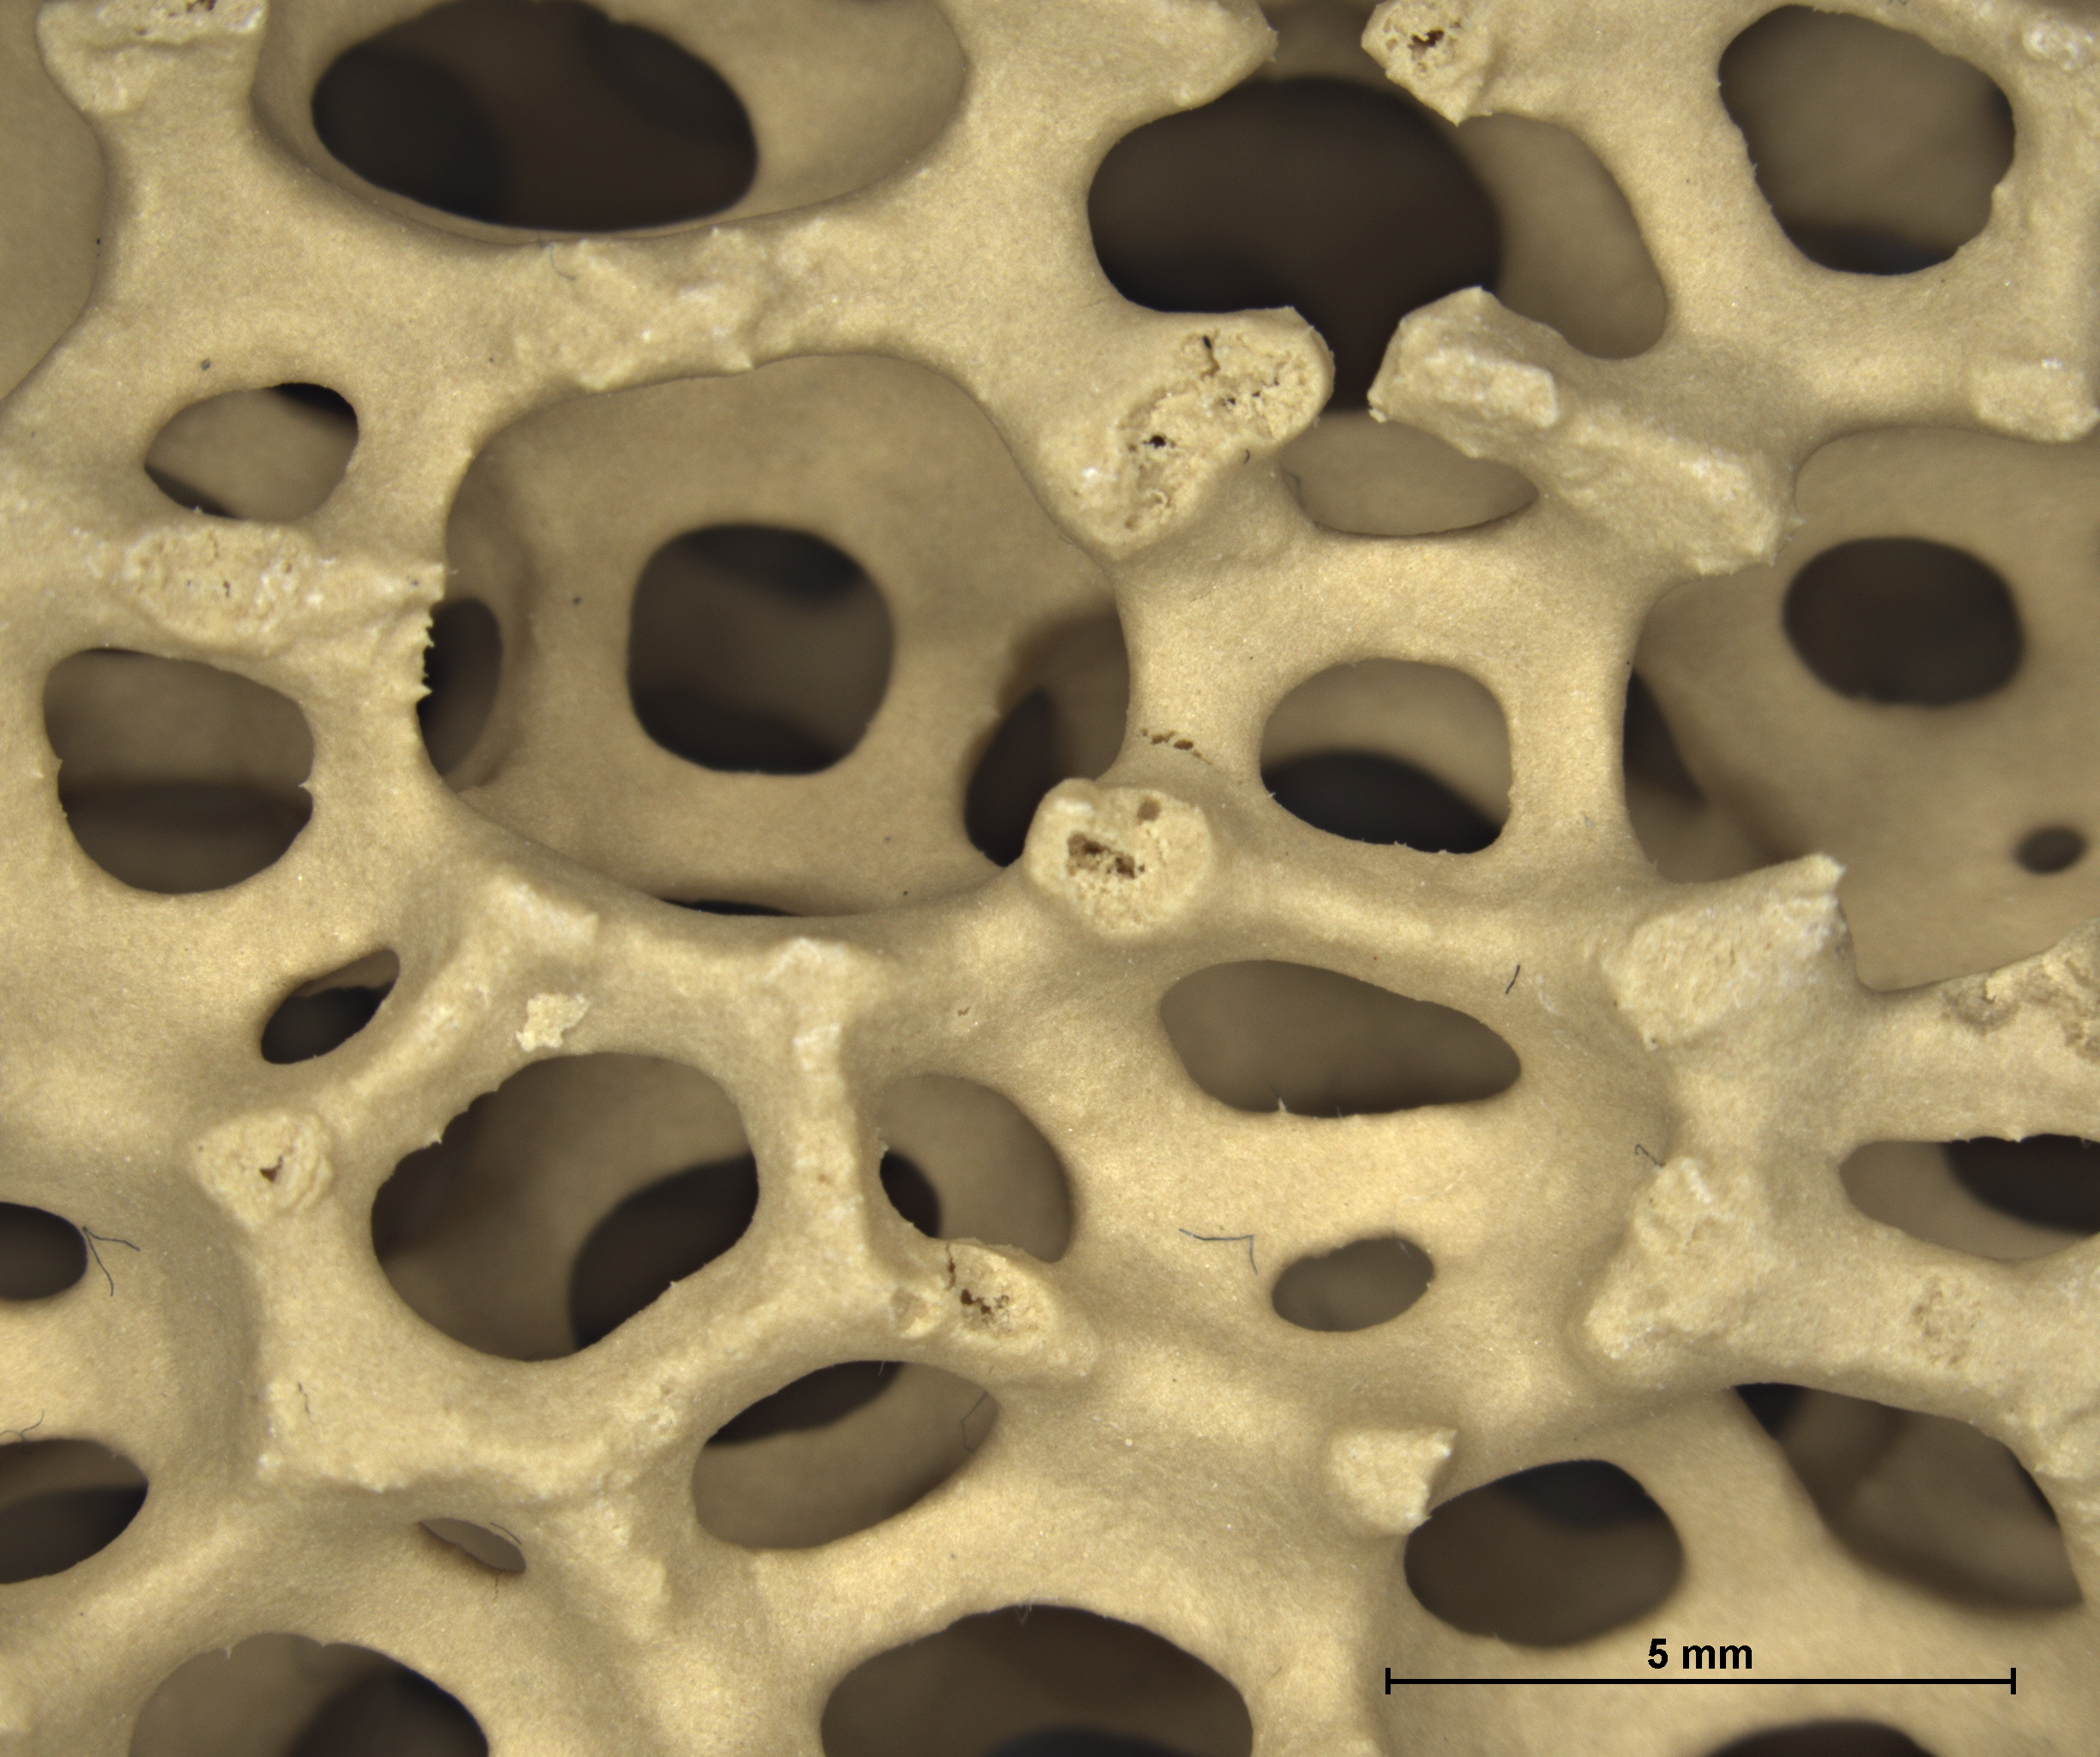
\includegraphics[width=\linewidth]{C3.jpg}
\caption{Sample C3}
\end{subfigure}
\hfill
\begin{subfigure}{0.45\textwidth}
\centering
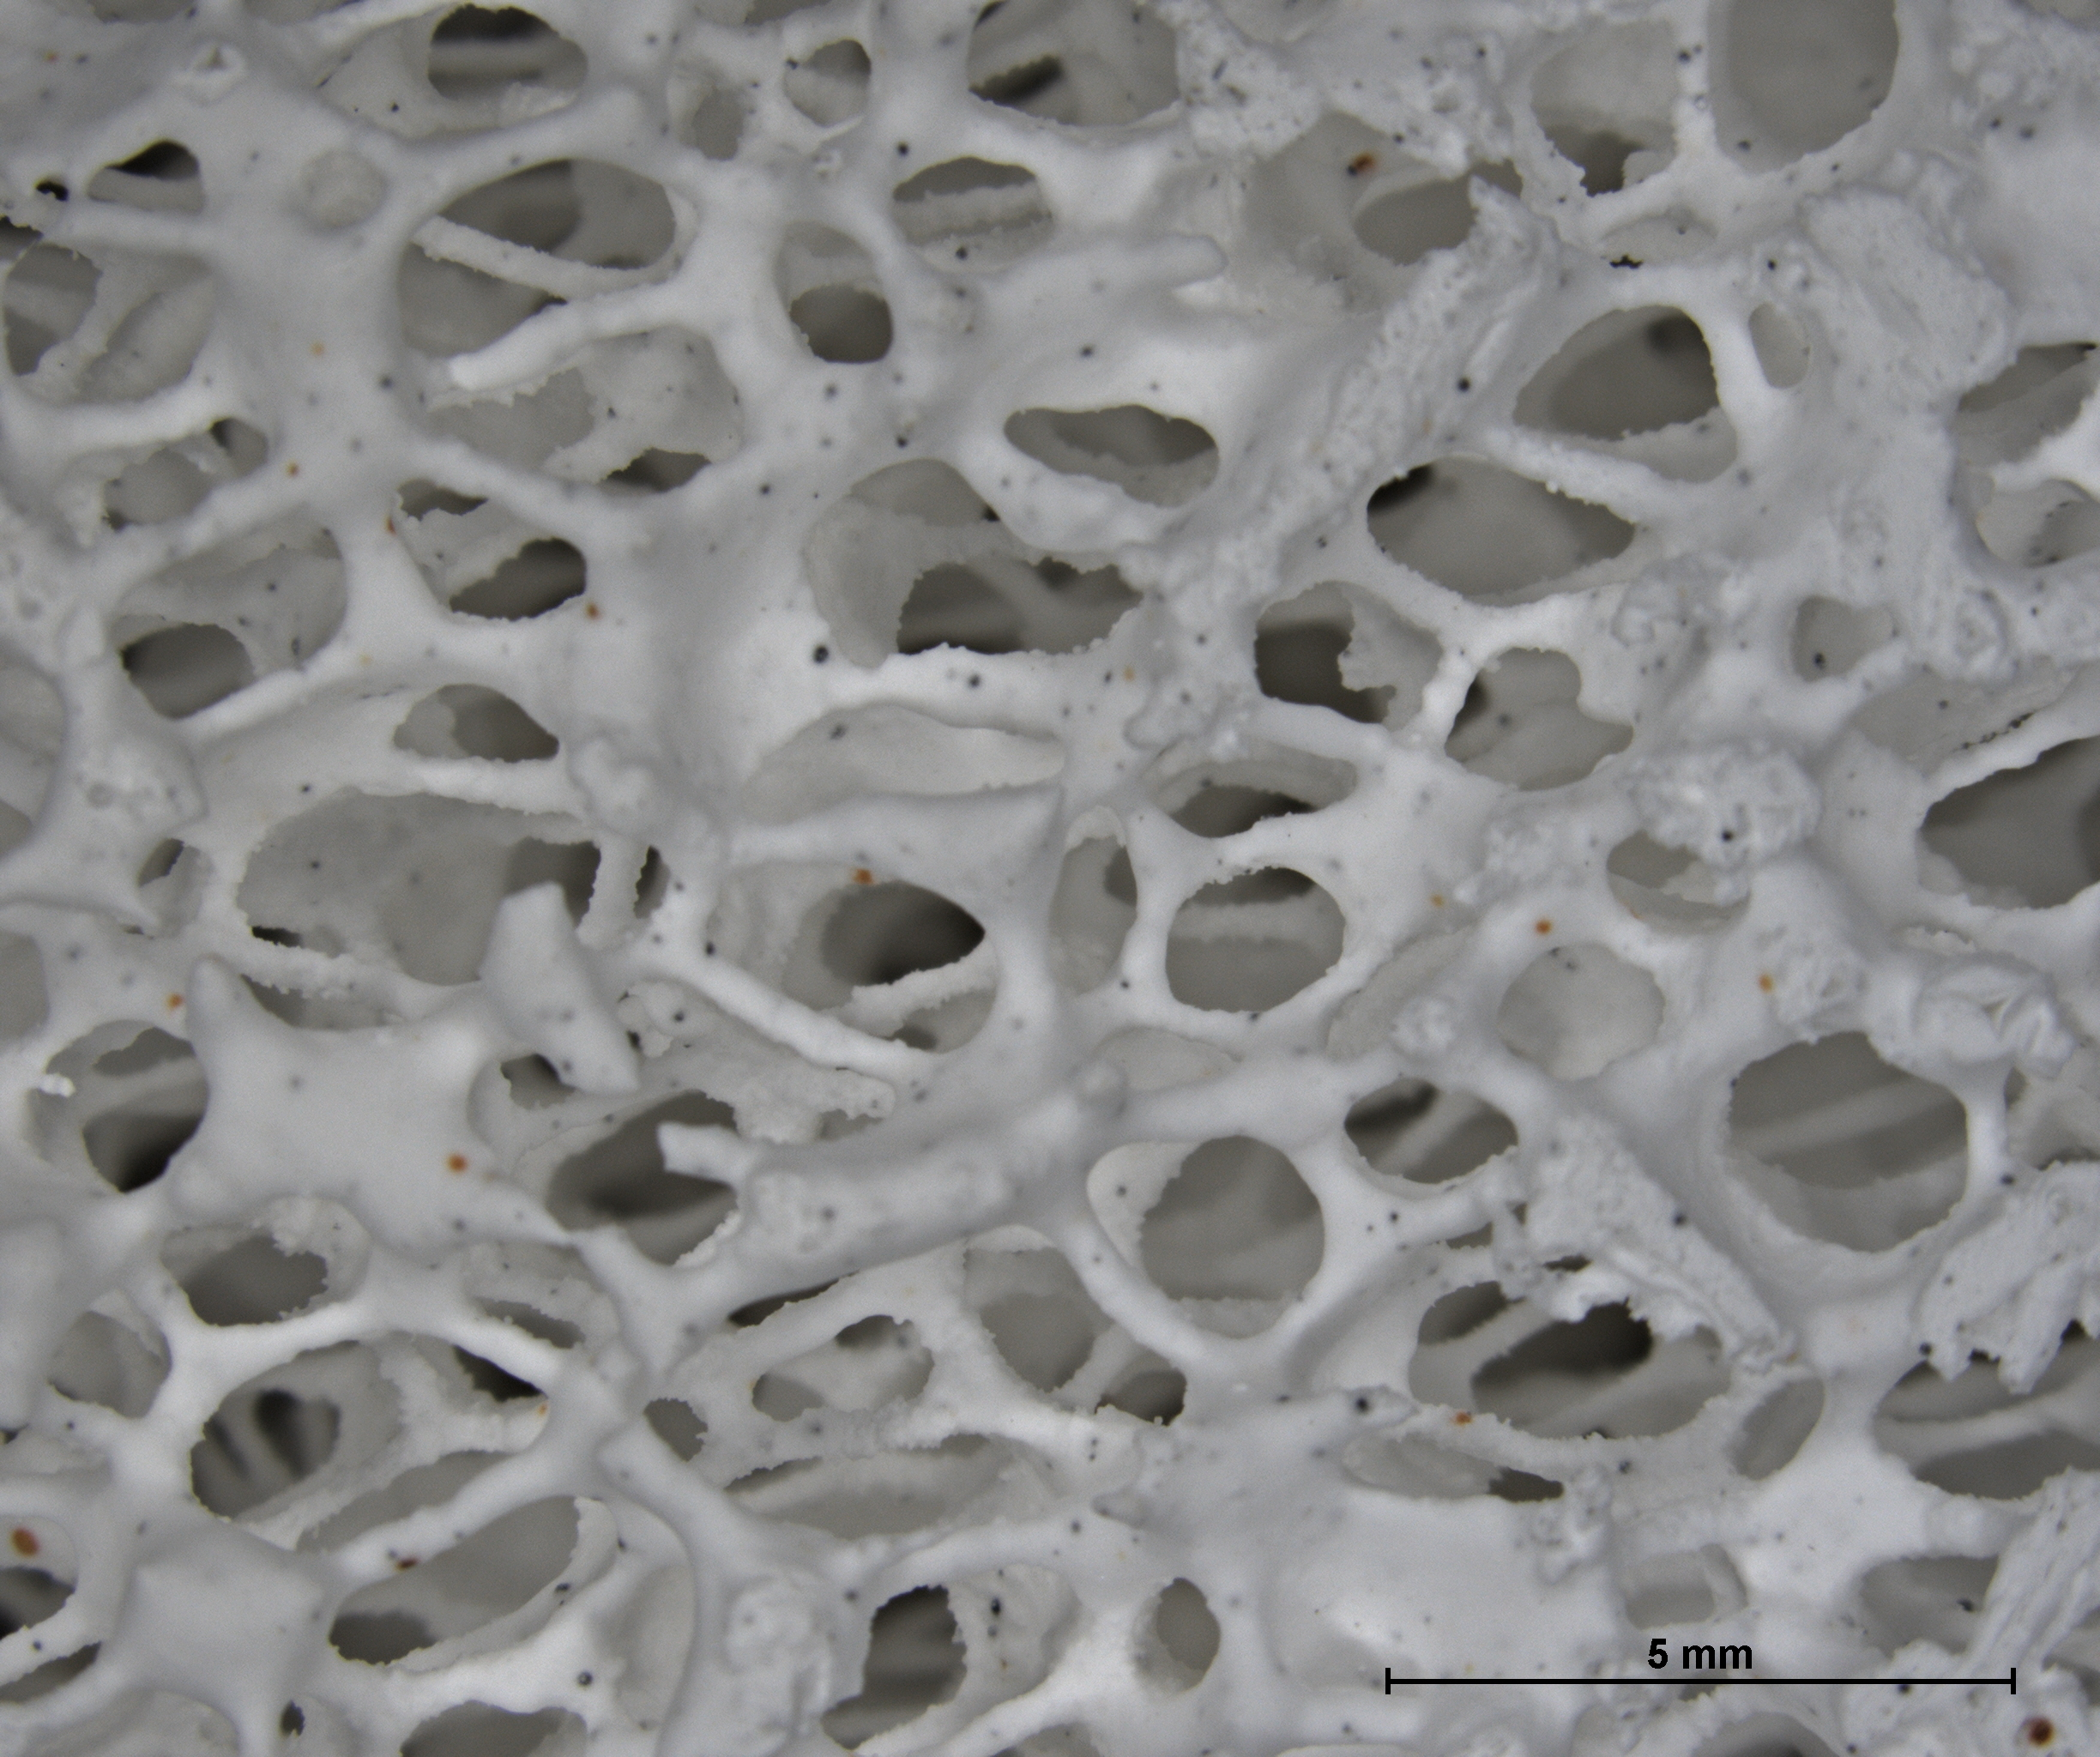
\includegraphics[width=\linewidth]{D1.jpg}
\caption{Sample D1}
\end{subfigure}

\vspace{0.4cm}


\begin{subfigure}{0.45\textwidth}
\centering
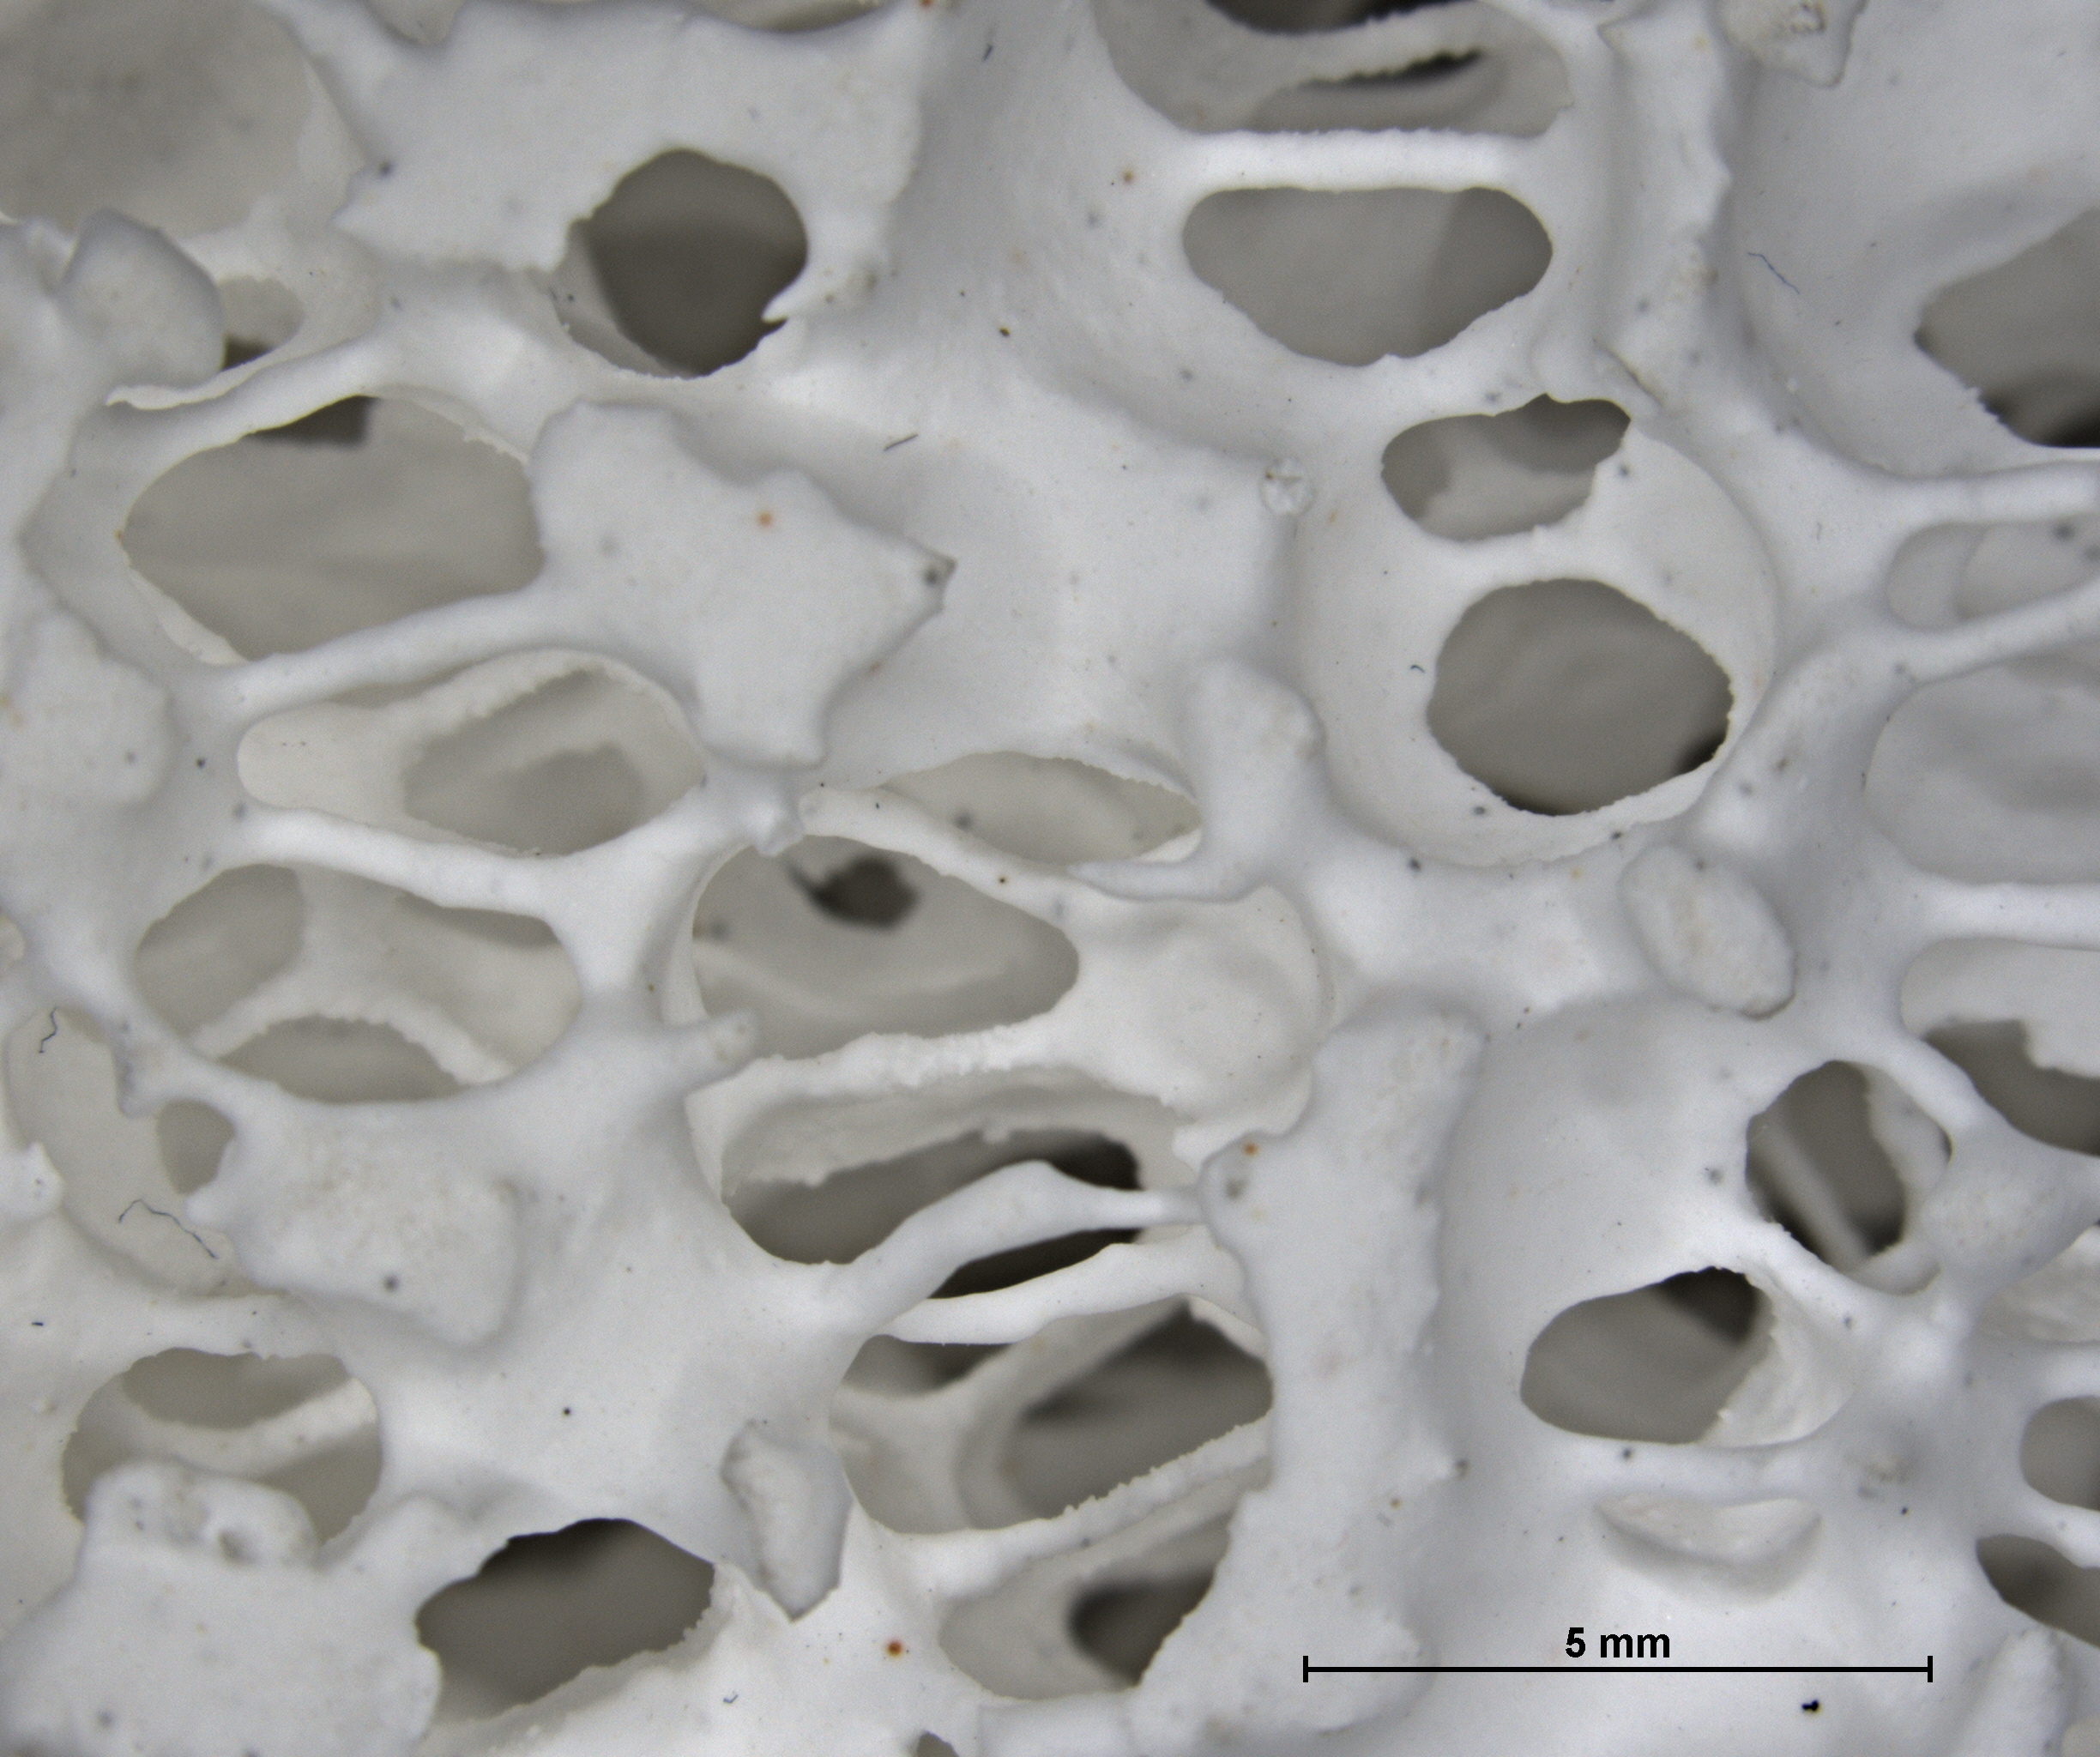
\includegraphics[width=\linewidth]{D2.jpg}
\caption{Sample D2}
\end{subfigure}
\hfill
\begin{subfigure}{0.45\textwidth}
\centering
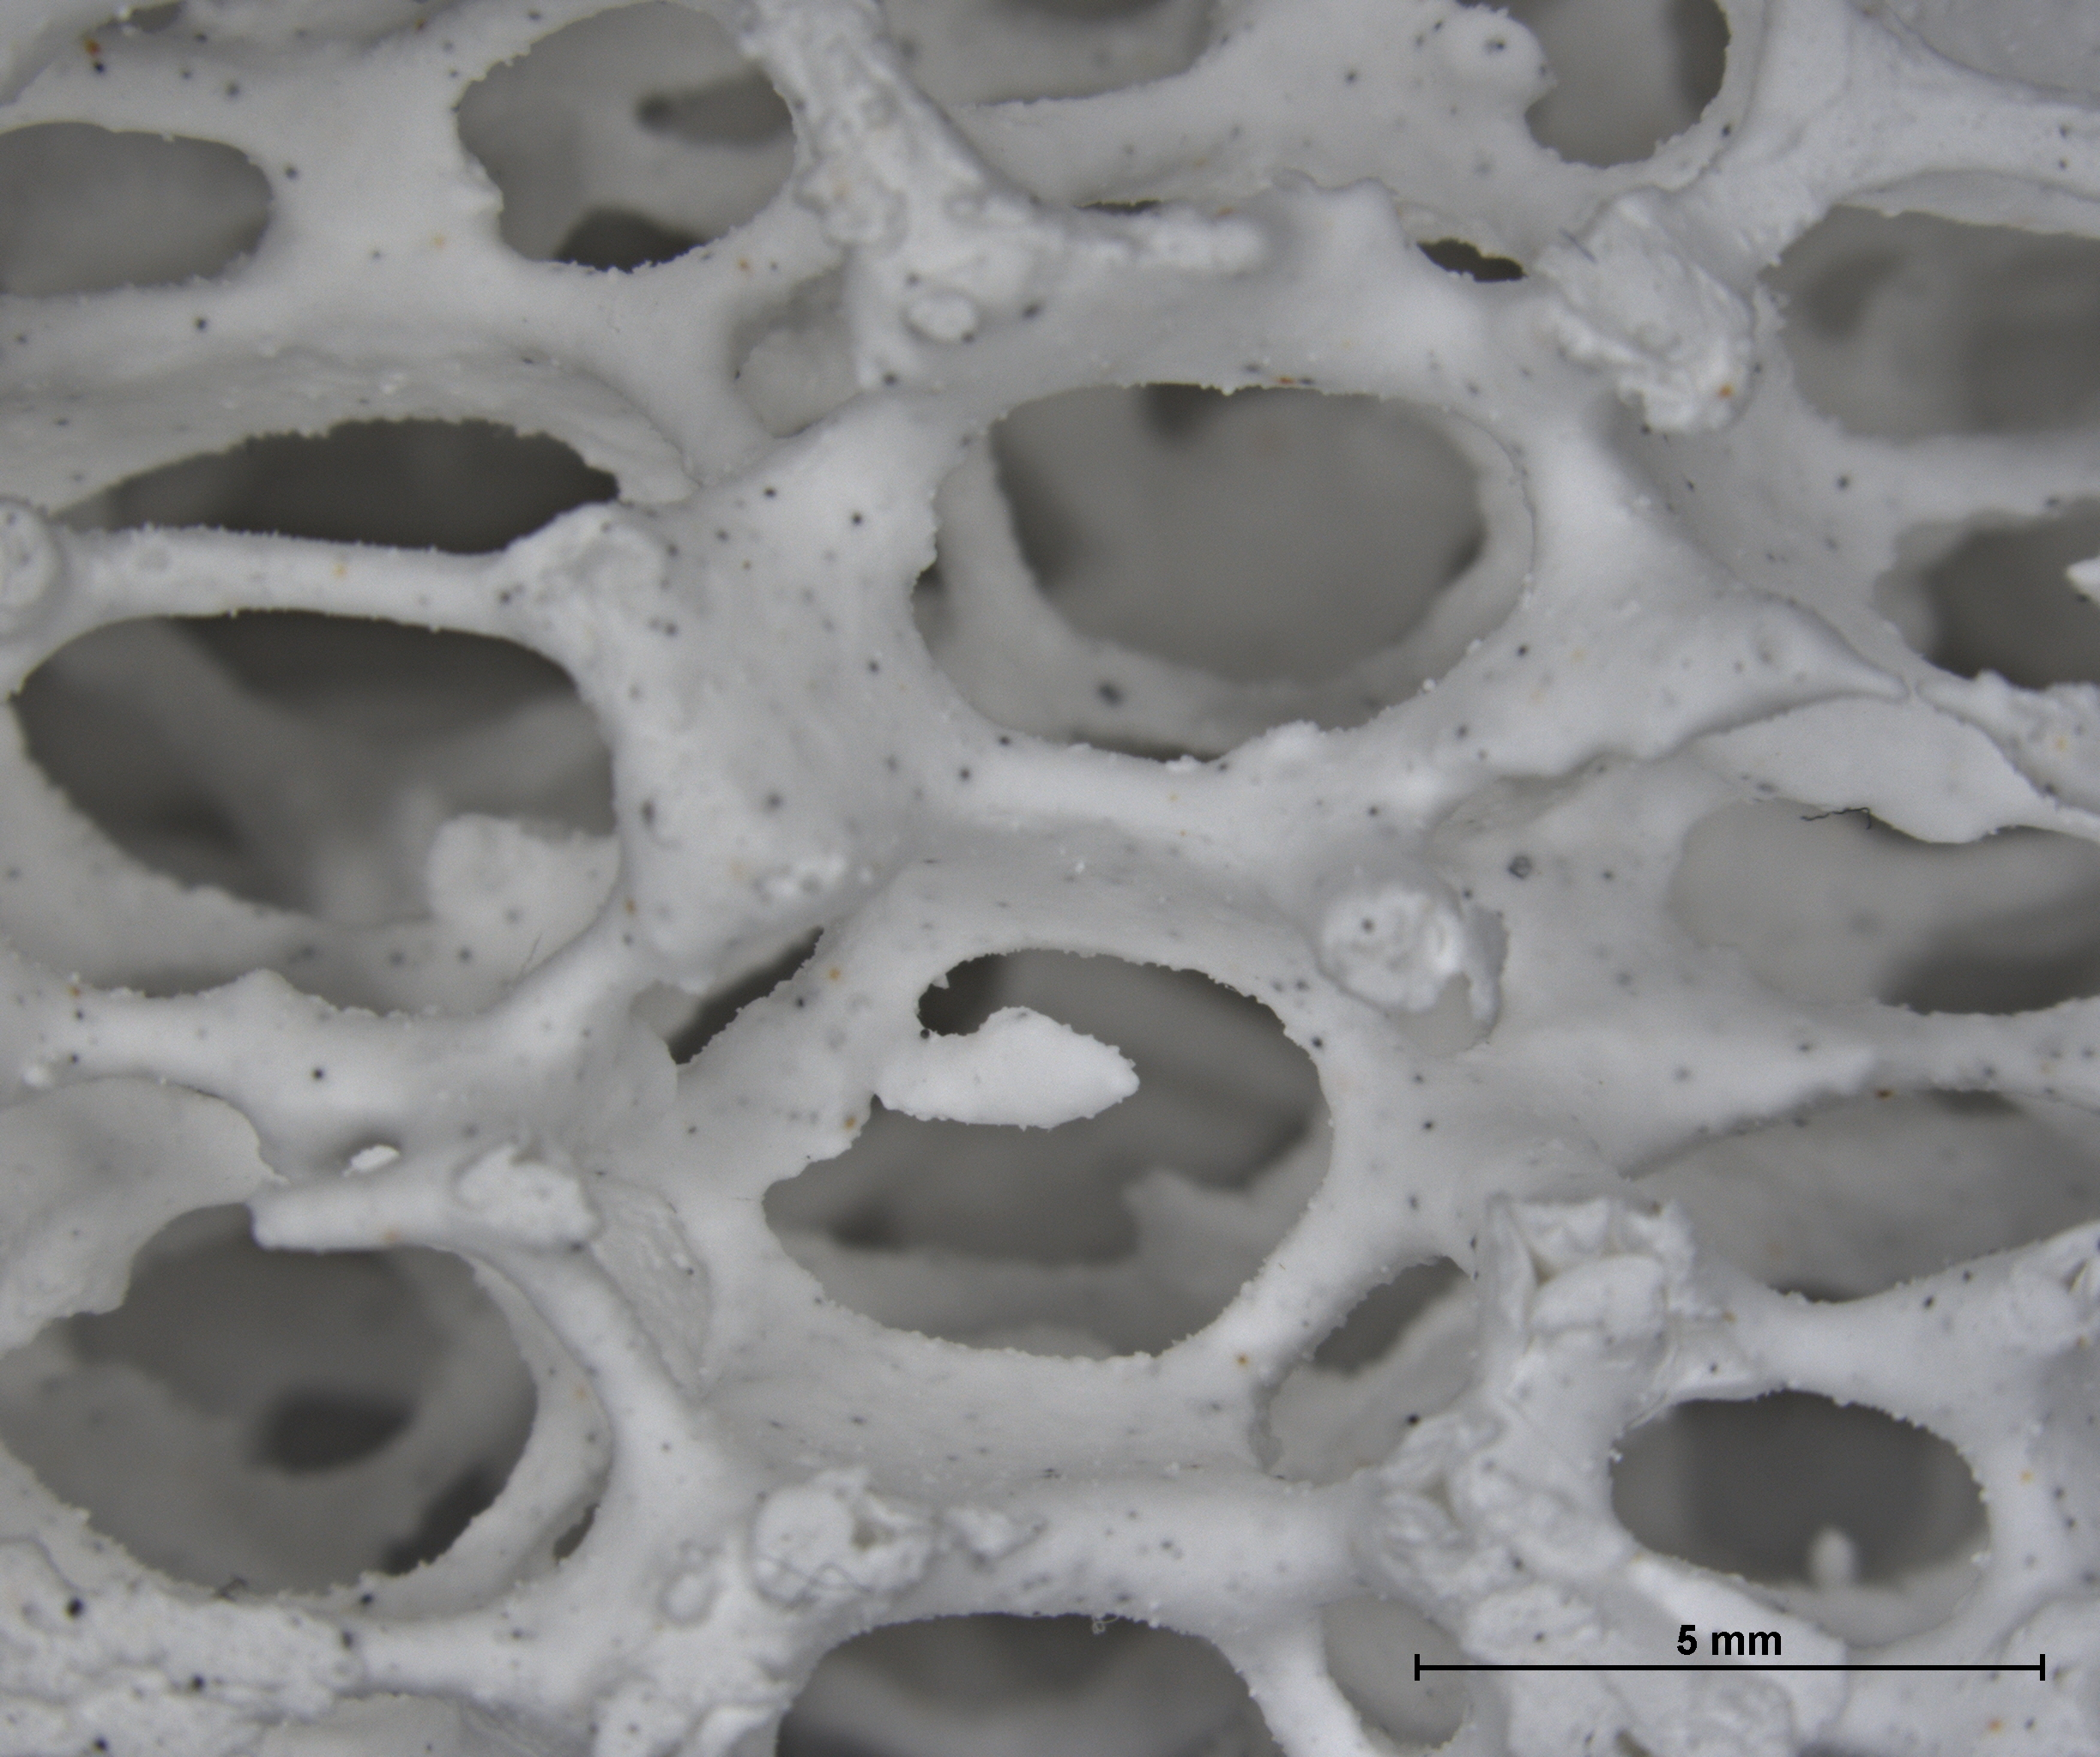
\includegraphics[width=\linewidth]{D3.jpg}
\caption{Sample D3}
\end{subfigure}

\caption{Porous material samples - Set 2}
\label{fig:sadavzorku2}
\end{figure}

\pagebreak

\begin{figure}[H]
\centering
\begin{subfigure}{0.45\textwidth}
\centering
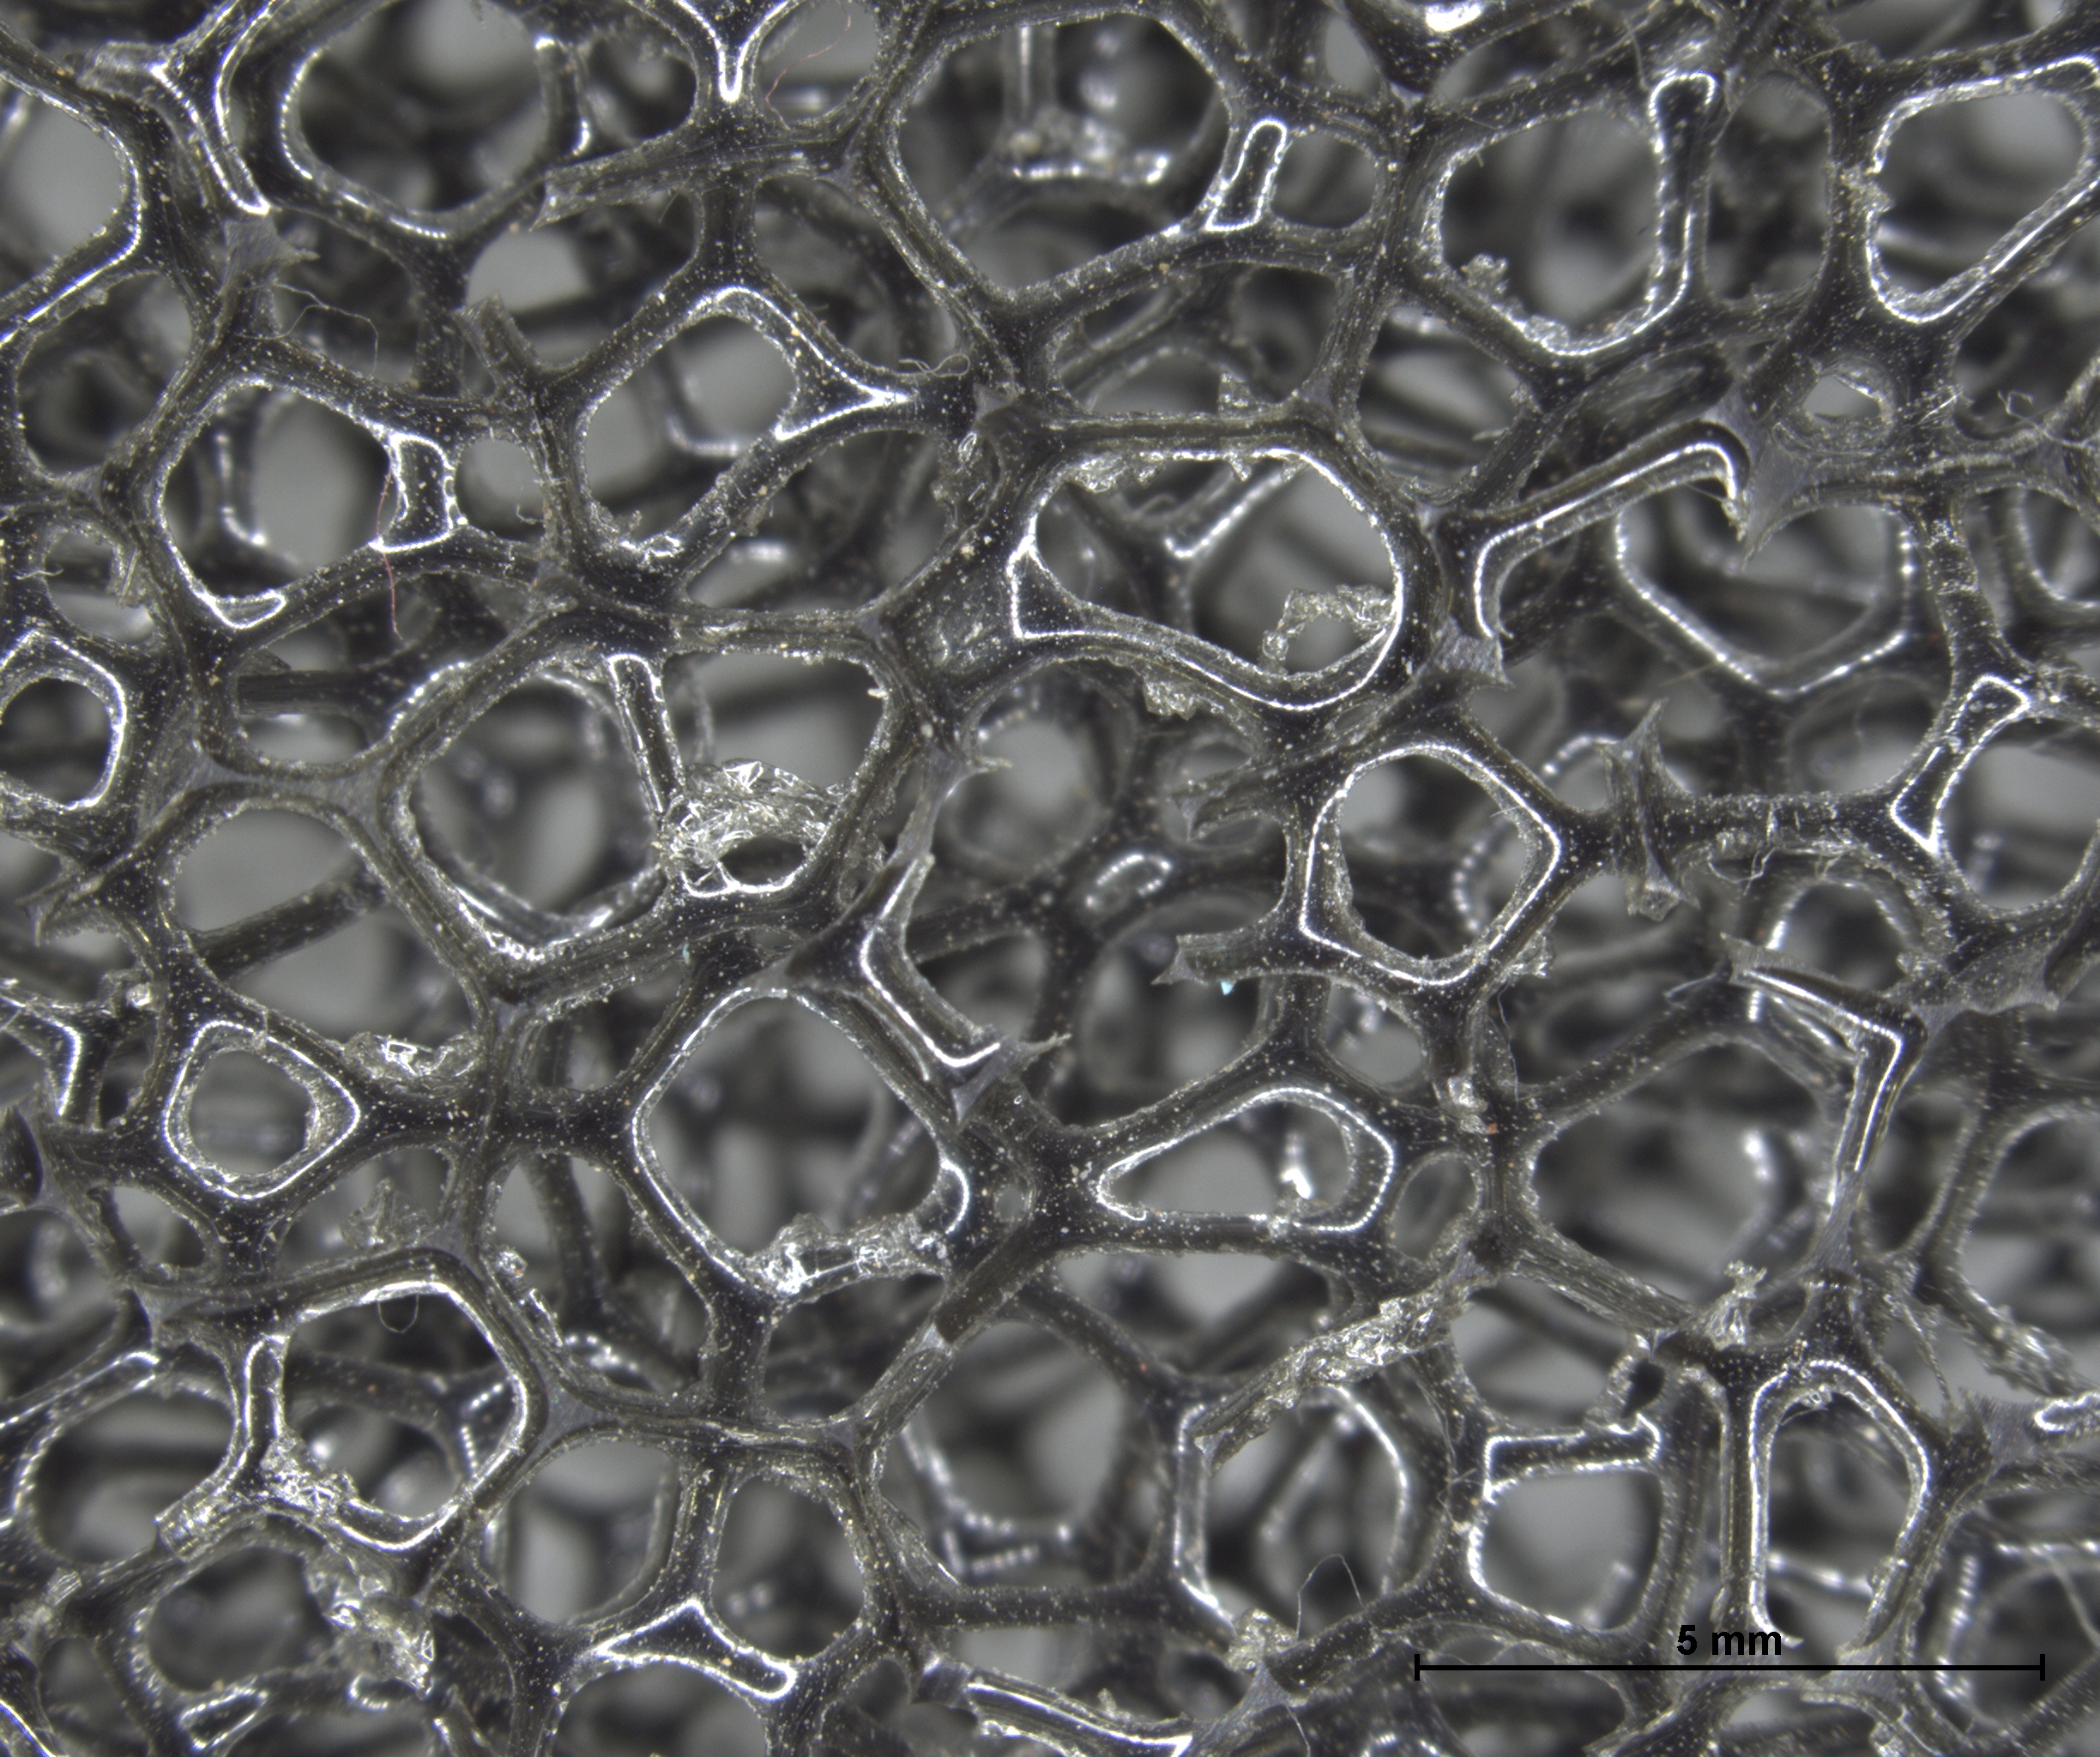
\includegraphics[width=\linewidth]{E1.jpg}
\caption{Sample E1}
\end{subfigure}
\hfill
\begin{subfigure}{0.45\textwidth}
\centering
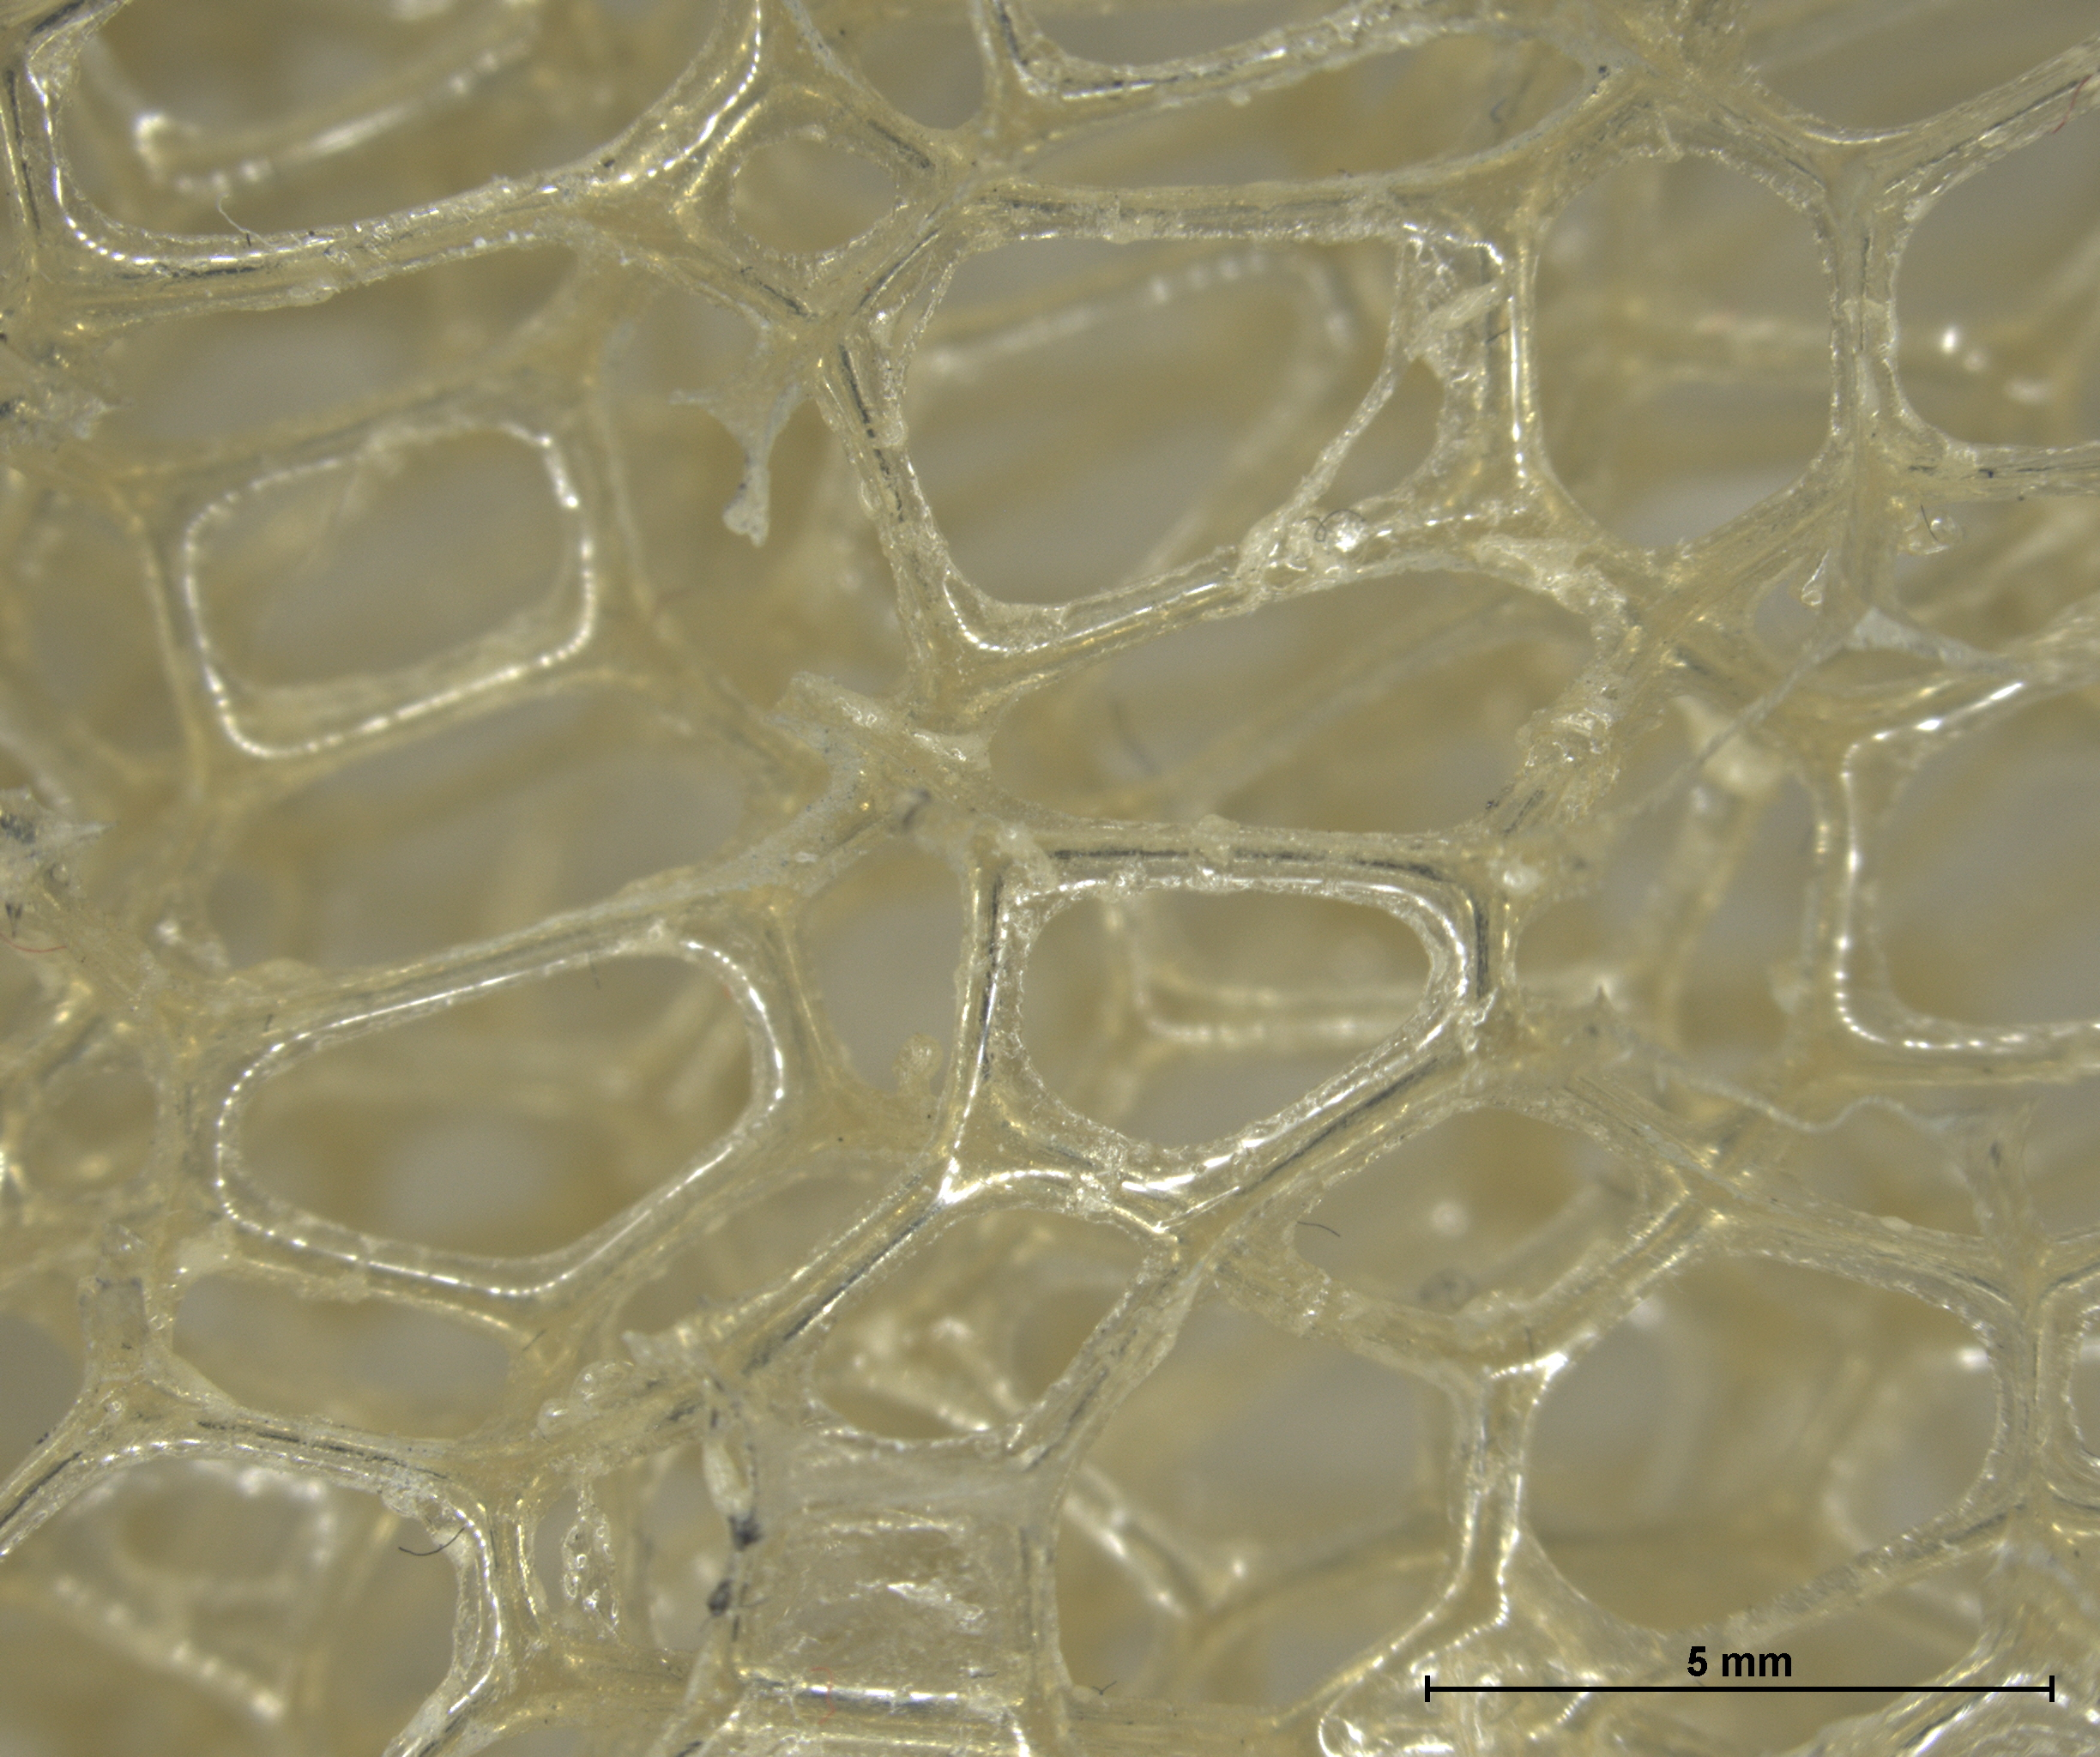
\includegraphics[width=\linewidth]{E2.jpg}
\caption{Sample E2}
\end{subfigure}

\caption{Porous material samples - Set 3}
\label{fig:sadavzorku3}
\end{figure}

\newpage
\subsection{Experimental results}

The following section presents the hydraulic performance of the investigated porous material samples obtained using the experimental facility described in the previous chapter. Pressure drop measurements were performed over a wide range of mass flow rates in order to quantify the flow resistance of each material and to evaluate the influence of pore morphology and material structure on hydraulic behaviour. The experimental results are first presented individually for each sample group, allowing direct comparison of materials with similar manufacturing characteristics. Subsequently, the measured data are analysed using the Darcy--Forchheimer approach to determine the permeability and inertial resistance coefficients, which are later compared with the numerical predictions and existing correlations reported in the literature.

\subsubsection{Pressure drop characteristics}
The measured pressure drop as a function of a flow velocity for the investigated porous materials is presented in Figures~\ref{fig:foam_results_A} and \ref{fig:foam_results_B}. Only sets A and B are presented in this section, all results are shown in Appendix B. To facilitate comparison, the results are grouped according to the individual sample sets introduced in the previous section. Each graph contains three specimens manufactured from the same material or using the same production route, allowing the influence of variations in the porous microstructure to be evaluated while minimizing the effect of material composition. The pressure drop characteristics provide the primary experimental dataset used for the subsequent determination of permeability and the Forchheimer coefficient.

\begin{figure}[h]
  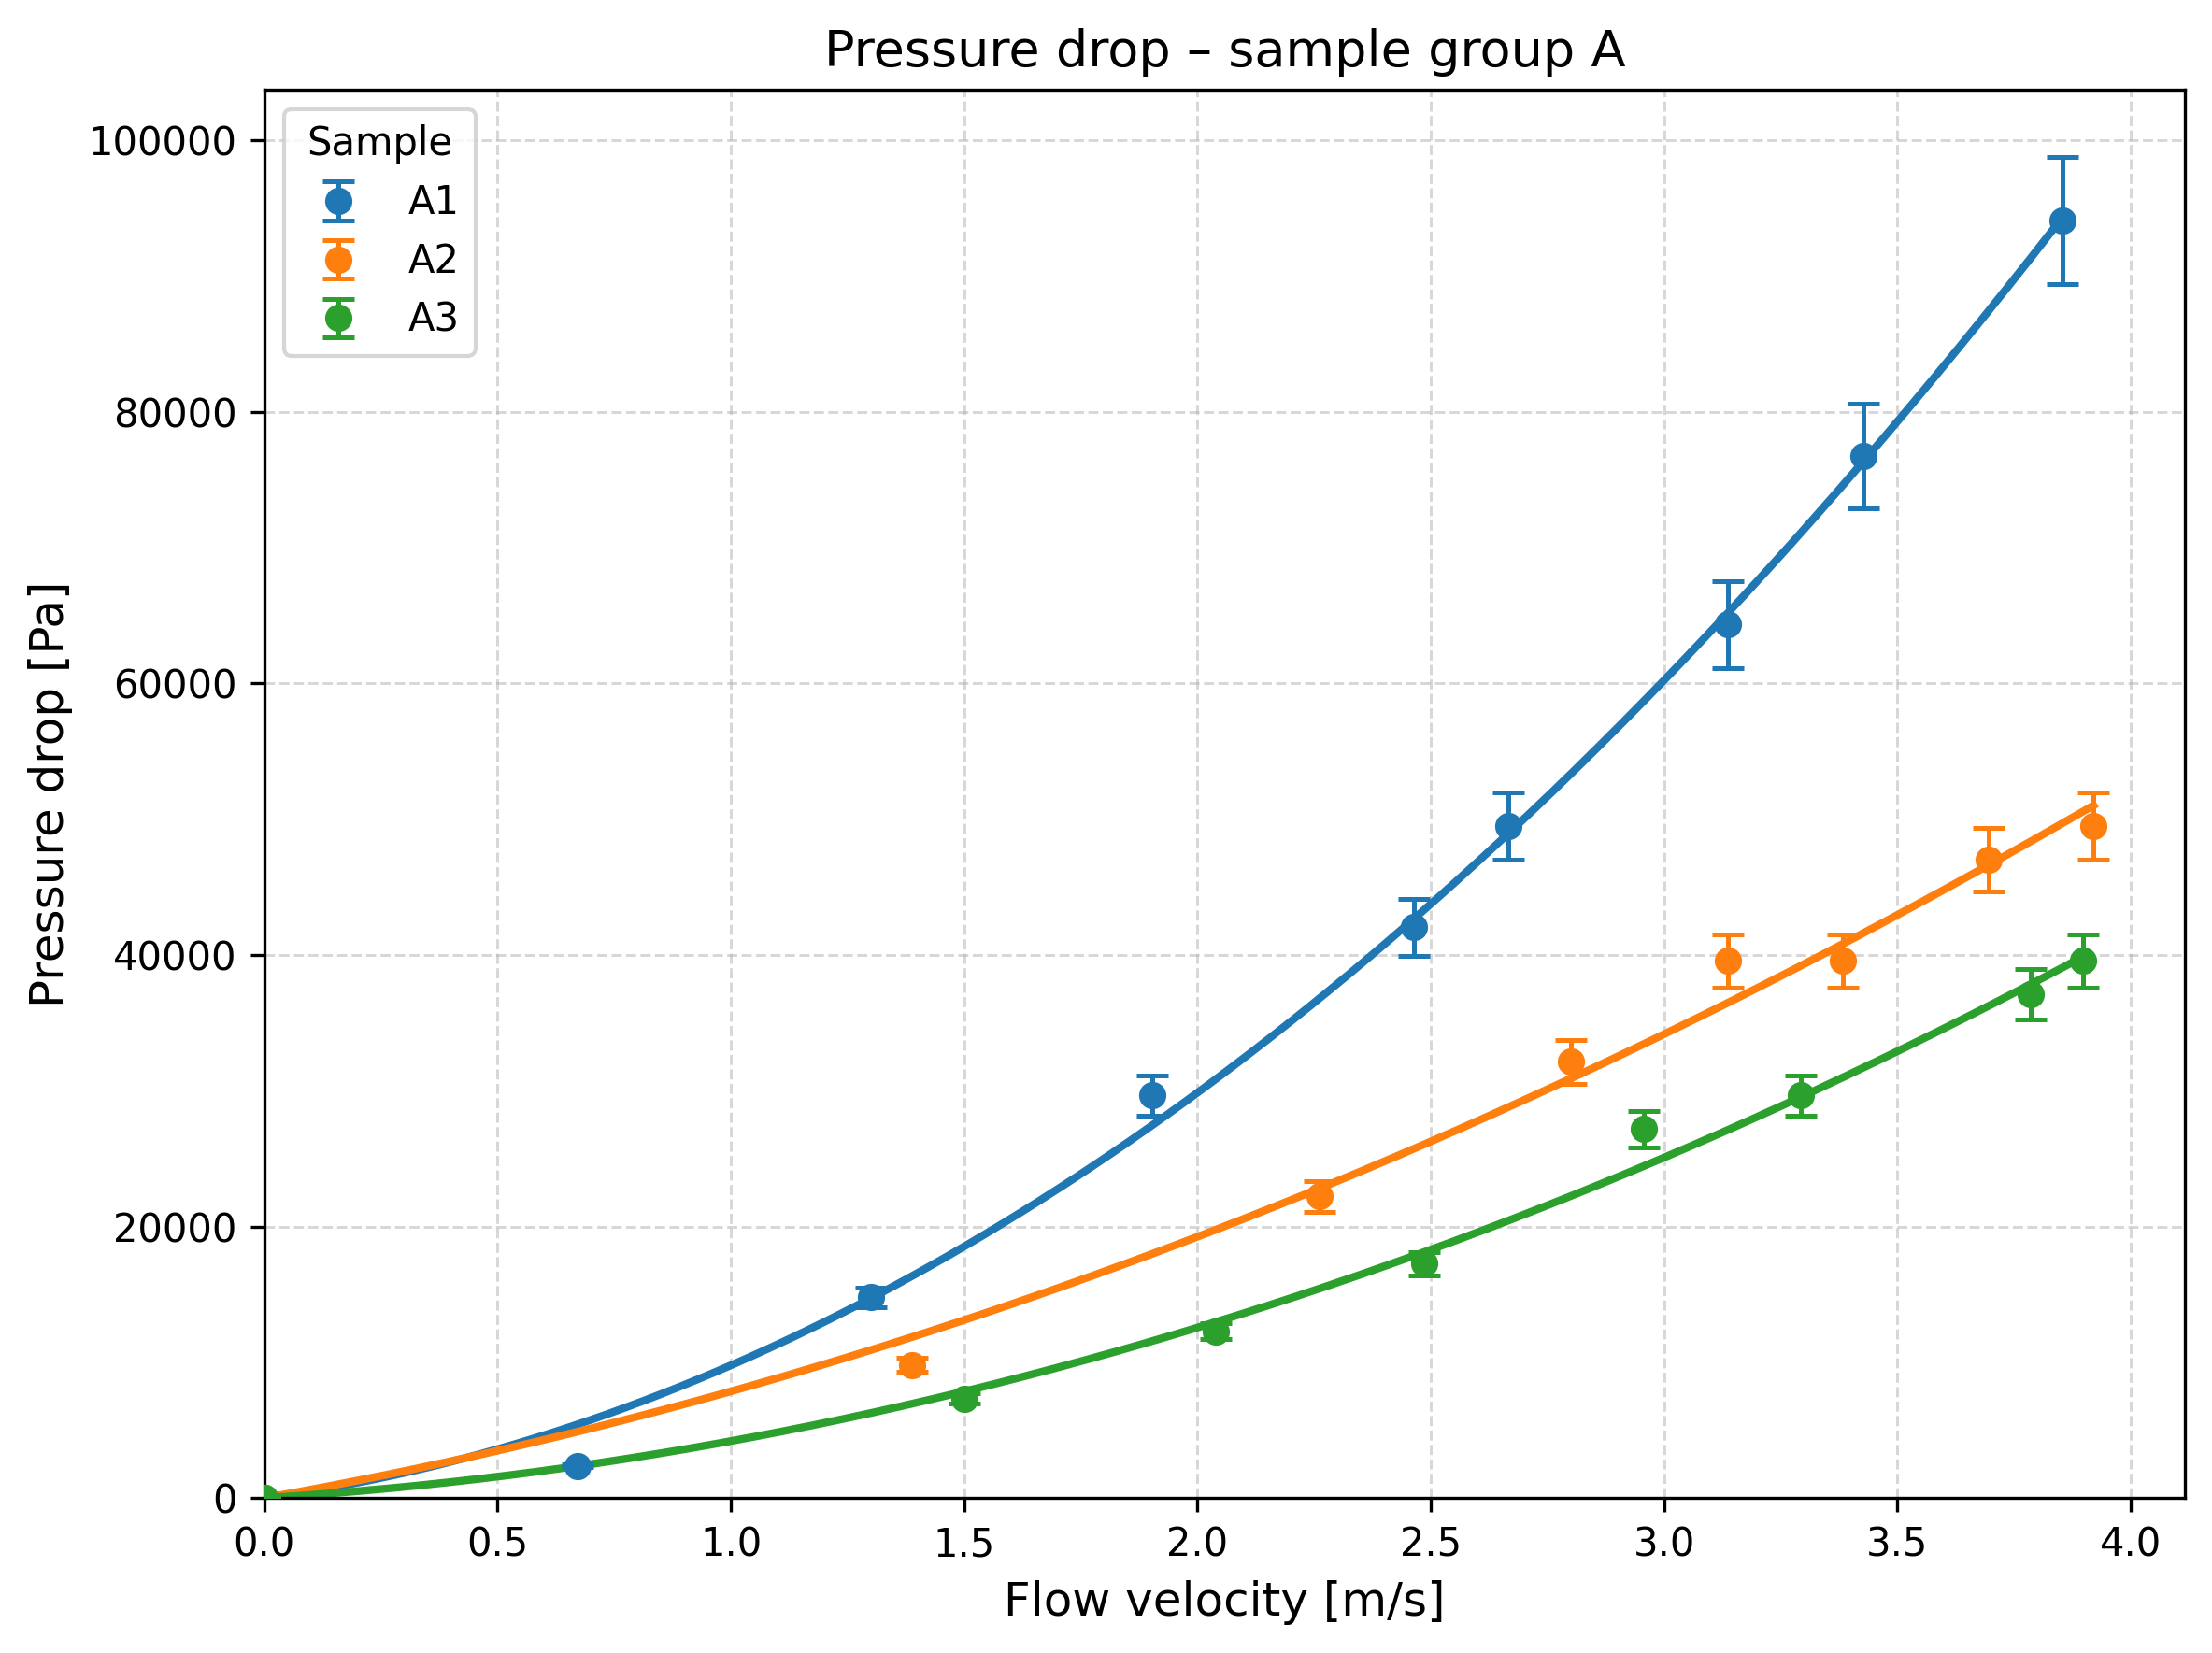
\includegraphics[width=13cm]{group_A_pressure_drop_velocity.png}
  \centering
  \caption{Pressure drop across the porous zone for the sample set A.}
  \label{fig:foam_results_A}
\end{figure}

\begin{figure}[h]
  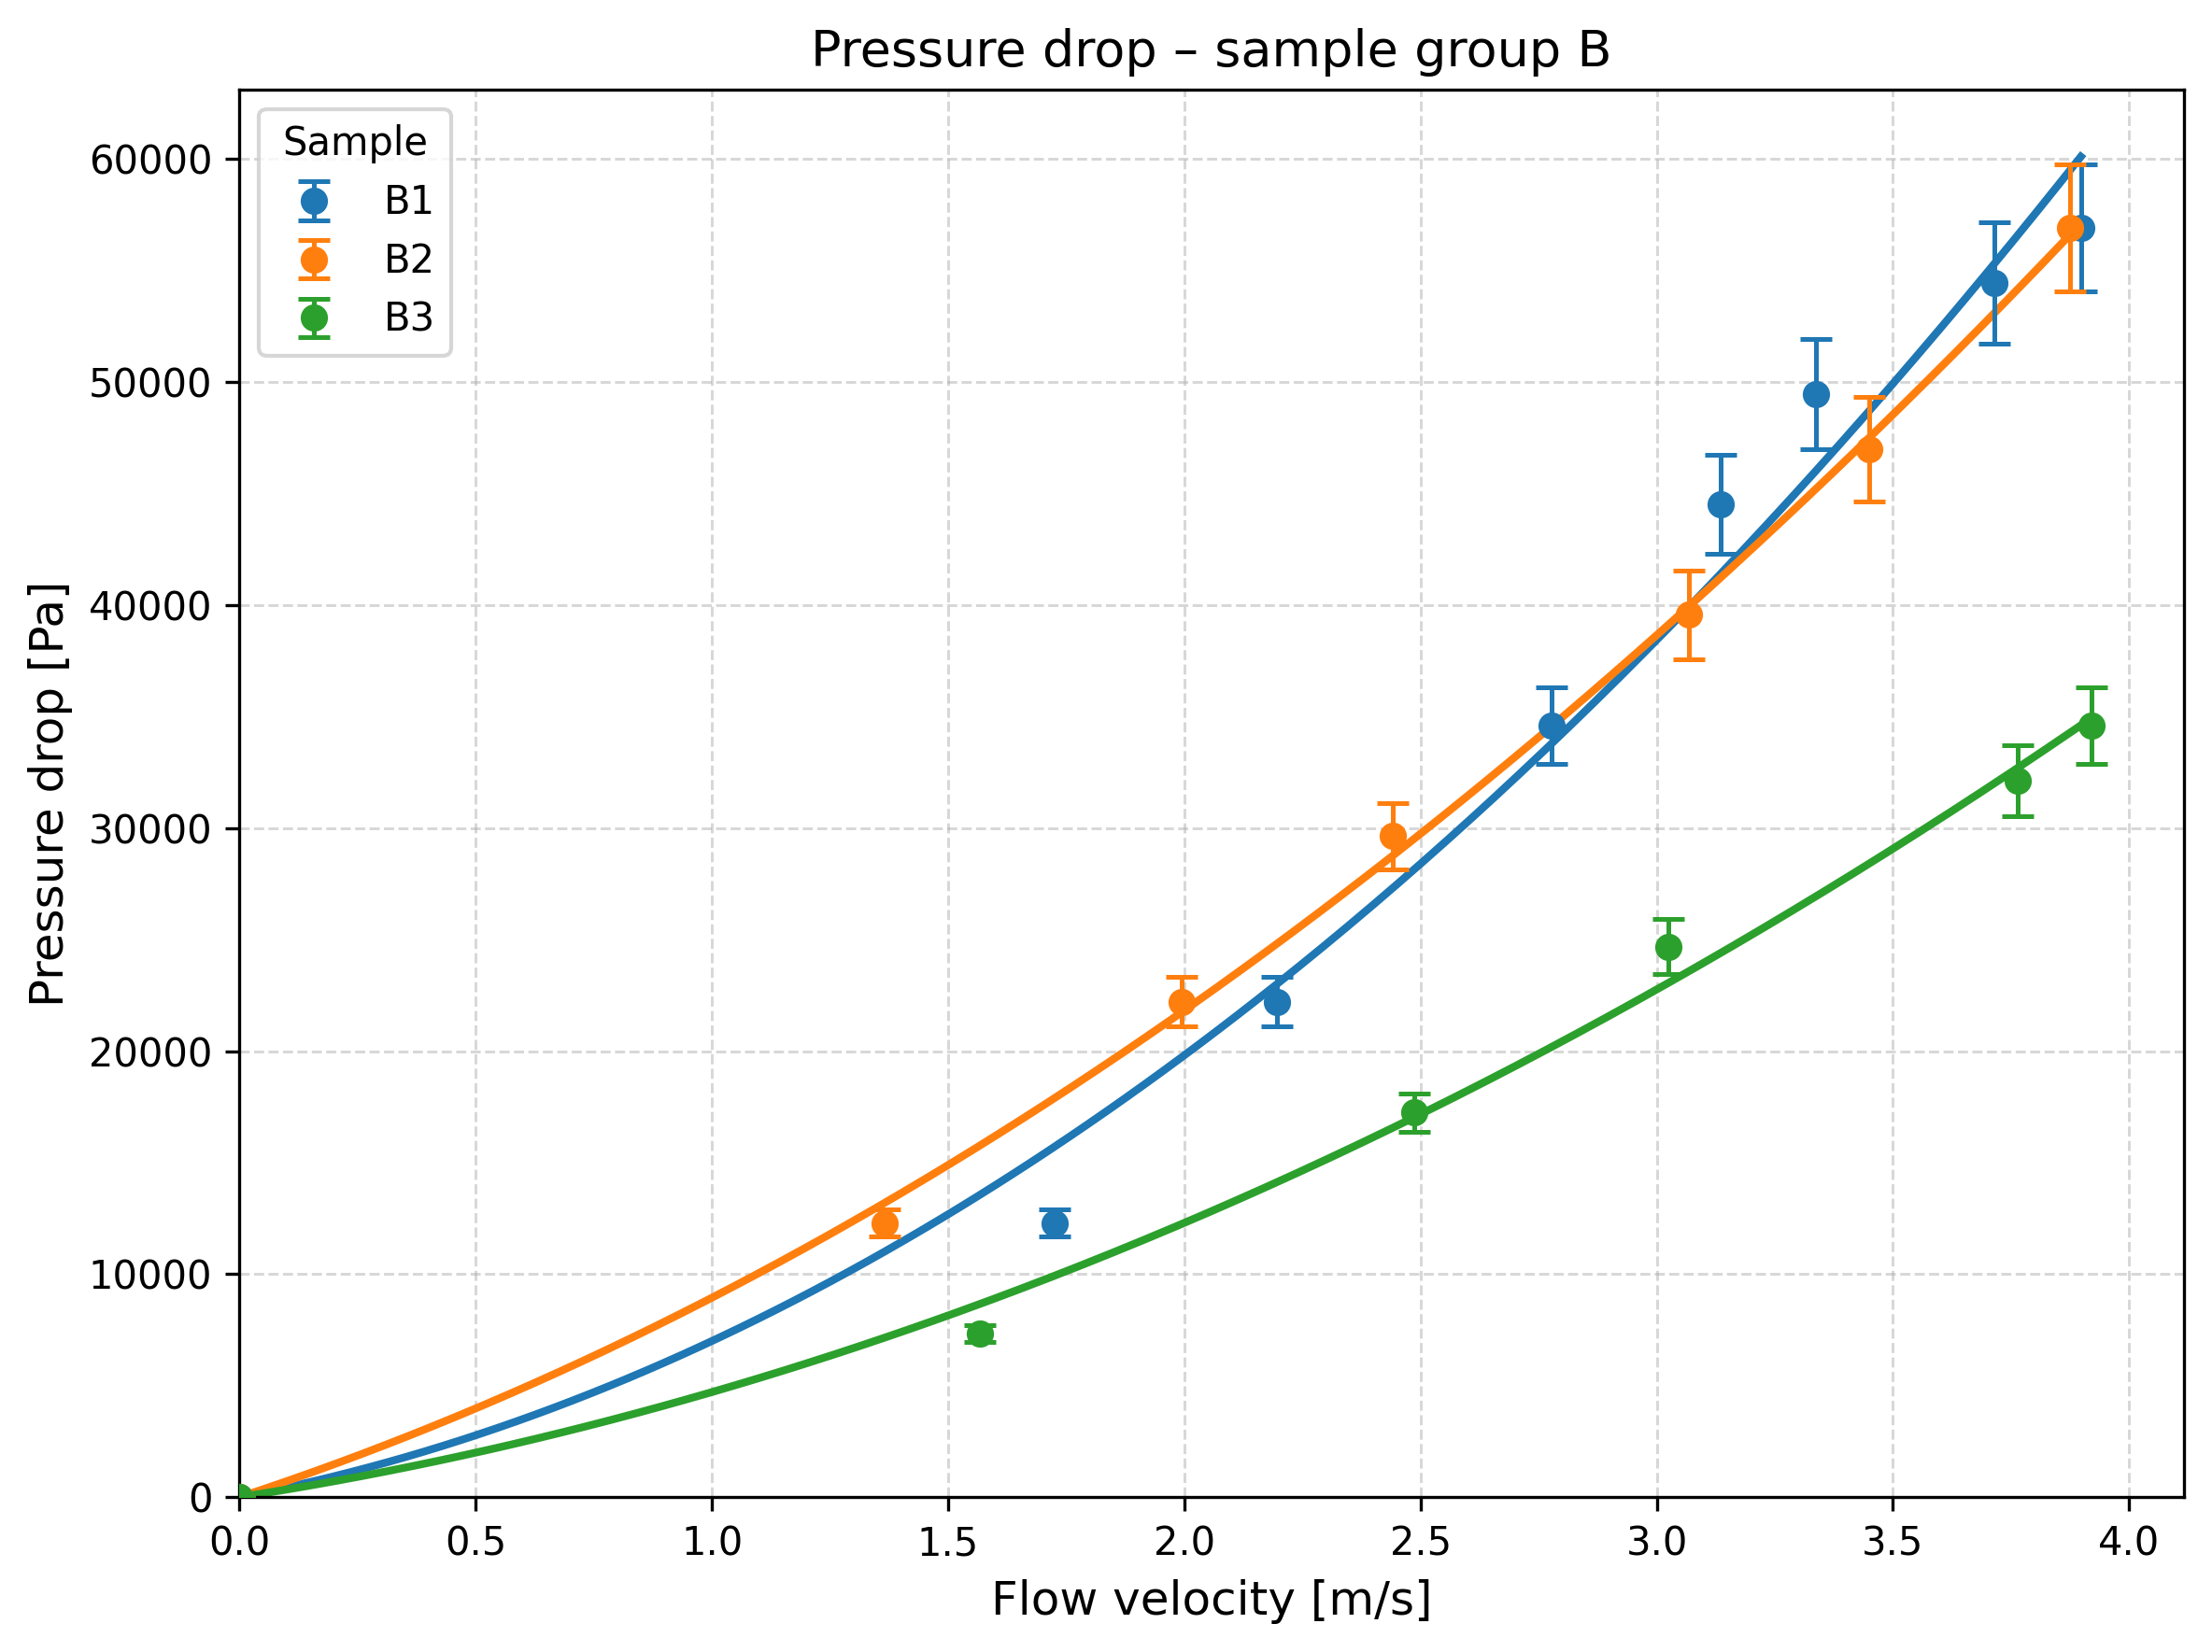
\includegraphics[width=13cm]{group_B_pressure_drop_velocity.png}
  \centering
  \caption{Pressure drop across the porous zone for the sample set B.}
  \label{fig:foam_results_B}
\end{figure}

\subsection{Processing and evaluation of the hydraulic measurements}
\label{sec:hydraulic_data_processing}

The measured pressure-drop data presented in the preceding section were further processed to obtain a quantitative description of the hydraulic resistance of the investigated porous samples. The measured mass flow rate was converted into the mean superficial flow velocity according to

\begin{equation}
    v = \frac{\dot{m}}{\rho A_{\mathrm{ch}}},
    \label{eq:superficial_velocity}
\end{equation}

where \(v\) is the superficial velocity, \(\dot{m}\) is the measured mass flow rate, \(\rho\) is the density of water, and \(A_{\mathrm{ch}}\) is the cross-sectional area of the test channel. In the present evaluation, a water density of \(998.2~\mathrm{kg\,m^{-3}}\) and a channel cross-section of \(40 \times 15~\mathrm{mm}\) were used.

\subsubsection{Darcy--Forchheimer approximation}
\label{subsec:darcy_forchheimer_approximation}

At sufficiently low flow velocities, flow through a porous medium can be described by Darcy's law, according to which the pressure gradient is directly proportional to the superficial velocity. At higher velocities, however, inertial effects associated with changes in flow direction, local accelerations, contractions, expansions, and flow separation within the pore network become significant. Under these conditions, the pressure drop is no longer proportional only to the first power of velocity, and the quadratic Forchheimer term must be included.

For steady one-dimensional flow through an isotropic porous medium, the Darcy--Forchheimer equation can be written as

\begin{equation}
    \frac{\Delta p}{L}
    =
    \frac{\mu}{K}v
    +
    \rho \beta v^2,
    \label{eq:darcy_forchheimer_gradient}
\end{equation}

where \(L\) is the porous-sample length, \(\mu\) is the dynamic viscosity of the fluid, \(K\) is the intrinsic permeability of the porous medium, \(\rho\) is the fluid density, and \(\beta\) is the Forchheimer coefficient. The first term on the right-hand side represents the viscous contribution to the pressure loss, whereas the second term represents the additional pressure loss caused by inertial effects.

For direct approximation of the measured pressure-drop data, Equation~\eqref{eq:darcy_forchheimer_gradient} was expressed in the following form:

\begin{equation}
    \Delta p = A v + B v^2,
    \label{eq:experimental_forchheimer_fit}
\end{equation}

where \(A\) and \(B\) are experimentally determined regression coefficients. Consequently, the intrinsic permeability and the dimensional Forchheimer coefficient can be calculated as

\begin{equation}
    K = \frac{\mu L}{A},
    \label{eq:permeability_from_A}
\end{equation}

and

\begin{equation}
    \beta = \frac{B}{\rho L}.
    \label{eq:forchheimer_from_B}
\end{equation}

The coefficient \(A\) therefore characterizes the linear viscous resistance of the entire tested sample. A lower value of \(A\) corresponds to a higher permeability, provided that the sample length and fluid viscosity remain constant. The coefficient \(B\) characterizes the nonlinear inertial contribution to the pressure drop. A higher value of \(B\) indicates a stronger increase in hydraulic resistance with increasing velocity.

It should be emphasized that \(A\) is not the permeability itself and \(B\) is not directly the Forchheimer coefficient. Both coefficients contain the effect of the sample length and, in the case of \(A\), also the fluid viscosity. Nevertheless, when all samples have the same length and are tested with the same fluid under comparable temperature conditions, the fitted coefficients can be directly used for a relative comparison of their hydraulic behaviour.

\subsubsection{Regression procedure}
\label{subsec:regression_procedure}

The measured data for each sample were fitted independently using Equation~\eqref{eq:experimental_forchheimer_fit}. No constant pressure-offset term was included in the regression. The fitted curve was therefore constrained to pass through the origin:

\begin{equation}
    \Delta p(v=0)=0.
\end{equation}

This condition is physically consistent because no flow-induced pressure loss can exist at zero flow velocity. In addition, both regression coefficients were constrained to non-negative values,

\begin{equation}
    A \geq 0,
    \qquad
    B \geq 0,
\end{equation}

in order to prevent non-physical decreasing or negative pressure-drop curves. The coefficients were obtained using a bounded least-squares procedure.

The agreement between the measured pressure drops and the fitted curves was evaluated using the coefficient of determination,

\begin{equation}
    R^2
    =
    1-
    \frac{
        \sum_{i=1}^{n}
        \left(
            \Delta p_i-\Delta p_{i,\mathrm{fit}}
        \right)^2
    }{
        \sum_{i=1}^{n}
        \left(
            \Delta p_i-\overline{\Delta p}
        \right)^2
    },
    \label{eq:r_squared}
\end{equation}

where \(\Delta p_i\) is the measured pressure drop, \(\Delta p_{i,\mathrm{fit}}\) is the pressure drop predicted by the fitted Darcy--Forchheimer relationship, and \(\overline{\Delta p}\) is the mean measured pressure drop.

The experimental points in the pressure-drop plots were supplemented by vertical error bars corresponding to an estimated relative pressure-drop uncertainty of \(\pm 10\,\%\). These error bars were introduced to illustrate the assumed measurement uncertainty and the expected scatter of the experimental data. They should therefore be interpreted as an estimated relative uncertainty rather than as a confidence interval obtained from repeated measurements.

\subsection{Fitted hydraulic coefficients}
\label{subsec:fitted_hydraulic_coefficients}

Table~\ref{tab:darcy_forchheimer_coefficients} summarizes the fitted coefficients \(A\) and \(B\), together with the corresponding coefficients of determination. The values were obtained from the same approximations as those used to generate the curves shown in the preceding graphical results.

\begin{table}[htbp]
    \centering
    \caption{Coefficients of the fitted Darcy--Forchheimer relationships
    \(\Delta p = Av + Bv^2\) for all investigated samples.}
    \label{tab:darcy_forchheimer_coefficients}

    \begin{tabular}{lccc}
        \hline
        \textbf{Sample}
        &
        \(\boldsymbol{A}\)
        \([\mathrm{Pa\,s\,m^{-1}}]\)
        &
        \(\boldsymbol{B}\)
        \([\mathrm{Pa\,s^2\,m^{-2}}]\)
        &
        \(\boldsymbol{R^2}\)
        \\
        \hline

        A1 & 4626.70 & 5149.64 & 0.9982 \\
        A2 & 6090.63 & 1765.38 & 0.9912 \\
        A3 & 2112.25 & 2082.14 & 0.9934 \\

        \hline

        B1 & 4095.22 & 2905.23 & 0.9852 \\
        B2 & 6971.14 & 1970.50 & 0.9990 \\
        B3 & 3272.14 & 1438.34 & 0.9948 \\

        \hline

        C1 & 0.00 & 1191.99 & 0.9277 \\
        C2 & 0.00 & 1403.90 & 0.9829 \\
        C3 & 0.00 & 1231.75 & 0.9691 \\

        \hline

        D1 & 109.12 & 1976.04 & 0.9965 \\
        D2 & 0.00 & 1784.36 & 0.9932 \\
        D3 & 0.00 & 1866.42 & 0.9898 \\

        \hline

        E1 & 1783.59 & 2768.57 & 0.9870 \\
        E2 & 0.00 & 1556.36 & 0.9735 \\

        \hline
    \end{tabular}
\end{table}

Values of \(A\) smaller than the numerical precision relevant to the present analysis were reported as zero. For example, the fitted values of \(A\) for samples C1, C2, C3, D2, D3, and E2 were of the order of \(10^{-16}\) to \(10^{-29}~\mathrm{Pa\,s\,m^{-1}}\). Such values have no practical physical significance and indicate that the bounded regression assigned almost the entire measured pressure loss to the quadratic contribution.

The quality of the fits was generally high. The coefficients of determination ranged from \(R^2=0.9277\) for sample C1 to \(R^2=0.9990\) for sample B2. Most samples reached values above \(R^2=0.98\), demonstrating that the quadratic Darcy--Forchheimer expression provides a suitable description of the measured relationship between superficial velocity and pressure drop within the investigated operating range.

The lowest value of \(R^2\) was obtained for sample C1. This sample contained only a limited number of measured points, and the measured pressure drops were relatively low compared with the other sample groups. Consequently, the resulting approximation was more sensitive to individual measurement deviations and to the resolution of the differential-pressure measurement system.

\subsection{Comparison of the sample groups}
\label{subsec:comparison_sample_groups}

The fitted coefficients reveal substantial differences in the hydraulic behaviour of the investigated porous structures. Samples A1 and A2 exhibited comparatively high values of the linear coefficient \(A\). This indicates a pronounced viscous contribution to their pressure losses and, assuming identical sample lengths, a lower permeability than that of samples characterized by smaller values of \(A\).

Sample B2 exhibited the largest linear coefficient,

\begin{equation}
    A_{\mathrm{B2}}
    =
    6971.14~\mathrm{Pa\,s\,m^{-1}},
\end{equation}

whereas samples C1--C3, D2, D3, and E2 produced values effectively equal to zero under the applied non-negative regression constraint. For these samples, the pressure-drop dependence was described almost entirely by the quadratic term over the measured velocity range.

The largest quadratic coefficient was found for sample A1,

\begin{equation}
    B_{\mathrm{A1}}
    =
    5149.64~\mathrm{Pa\,s^2\,m^{-2}},
\end{equation}

indicating the strongest increase in pressure loss with the square of the superficial velocity. In contrast, the lowest quadratic coefficient was obtained for sample C1,

\begin{equation}
    B_{\mathrm{C1}}
    =
    1191.99~\mathrm{Pa\,s^2\,m^{-2}}.
\end{equation}

The differences between \(A\) and \(B\) demonstrate that the individual porous structures cannot be ranked using only a single hydraulic parameter. A structure may exhibit a relatively high viscous resistance but a weaker inertial contribution or, conversely, a small linear resistance accompanied by a pronounced quadratic increase in pressure loss. Both terms must therefore be considered when evaluating the suitability of a porous structure for engineering applications.

For the samples with an approximately zero fitted \(A\), the result should not automatically be interpreted as infinite physical permeability. Instead, it indicates that the available measurements did not contain sufficient information to identify a statistically meaningful linear contribution independently from the quadratic contribution. This may occur when the lowest measured non-zero velocity is already outside the purely Darcy regime, when the pressure drop is close to the resolution limit of the sensor, or when only a small number of measurement points is available.

A more reliable determination of the intrinsic permeability would require additional measurements at lower flow velocities, where the linear Darcy contribution is dominant. The permeability could then be determined from the initial slope of the pressure-gradient curve, while the Forchheimer coefficient could subsequently be obtained from the nonlinear part of the measurements.

\subsubsection{Summary of the hydraulic evaluation}
\label{subsec:hydraulic_evaluation_summary}

The measured hydraulic data were successfully represented using the Darcy--Forchheimer relationship

\begin{equation}
    \Delta p = Av+Bv^2.
\end{equation}

The approximation was constrained to pass through the origin and to provide non-negative viscous and inertial coefficients. The resulting coefficients of determination show that the selected model describes the experimental pressure-drop curves with good accuracy for all investigated samples.

The coefficient \(A\) represents the linear viscous resistance of the tested sample and is inversely related to its intrinsic permeability. The coefficient \(B\) represents the nonlinear inertial contribution and is related to the Forchheimer coefficient. Their conversion into intrinsic material properties requires knowledge of the sample length and the thermophysical properties of the working fluid.

The obtained results demonstrate clear differences in hydraulic resistance among the investigated porous samples. These differences reflect variations in pore size, pore morphology, porosity, tortuosity, and flow-path constrictions. The fitted coefficients therefore provide a suitable quantitative basis for the subsequent comparison between the optically determined microstructural parameters and the measured hydraulic behaviour of the porous materials.
\newpage

\subsection{Discussion of results}

The hydraulic behaviour of porous materials is commonly described by the coefficients $A$ and $B$ of the Darcy--Forchheimer equation, representing the viscous and inertial contributions to the overall pressure loss. In an attempt to identify relationships between the hydraulic response and the measured microstructural properties, the fitted coefficients were compared with two basic geometric descriptors obtained from optical microscopy: porosity and the average equivalent pore diameter $d_e$. Since the investigated materials exhibit substantially different pore morphologies, the samples were divided into two groups. The first group consisted of metallic foams (Cu and Sn), while the second included ceramic and polymer foams (Al$_2$O$_3$, ZrO$_2$ and polyurethane), which share a similar cellular morphology but differ from metallic foams in their manufacturing process and internal structure.
\begin{figure}[h]
  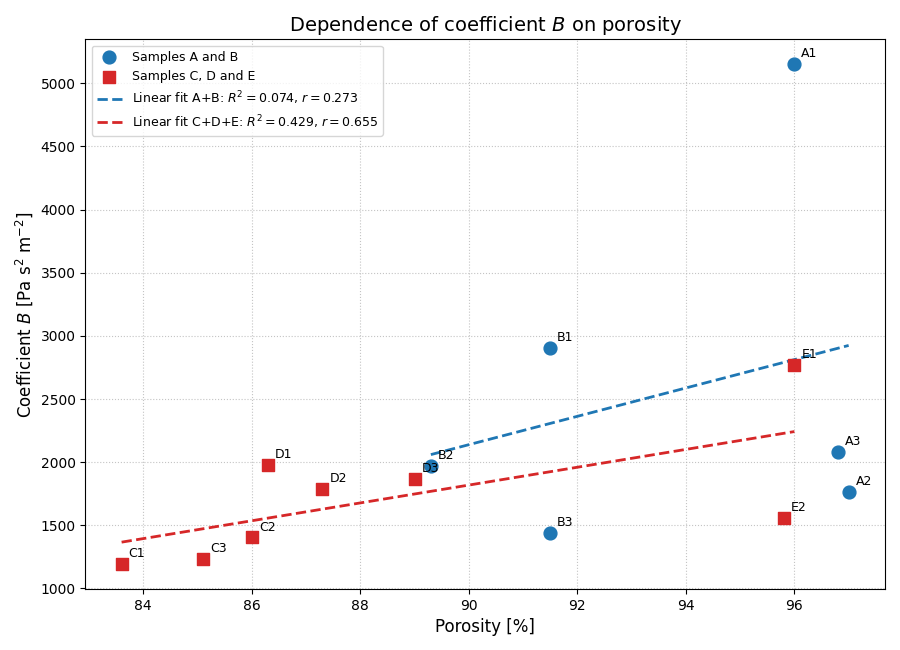
\includegraphics[width=14cm]{korelace_porozita.png}
  \centering
  \caption{Dependence of the inertial coefficient $B$ on the porosity.}
  \label{fig:B_porosity}
\end{figure}

Figure~\ref{fig:B_porosity} compares the inertial coefficient $B$ with the measured porosity. Although a slight trend can be observed within individual material groups, the overall correlation remains weak. Samples possessing nearly identical porosity frequently exhibit significantly different values of the pressure-loss coefficient. This indicates that porosity alone cannot adequately describe the hydraulic resistance of open-cell porous materials. While porosity determines the overall void fraction available for the flow, it does not capture the internal topology of the pore network, such as pore interconnections, constrictions or tortuosity, which strongly influence the flow field.

\begin{figure}[h]
  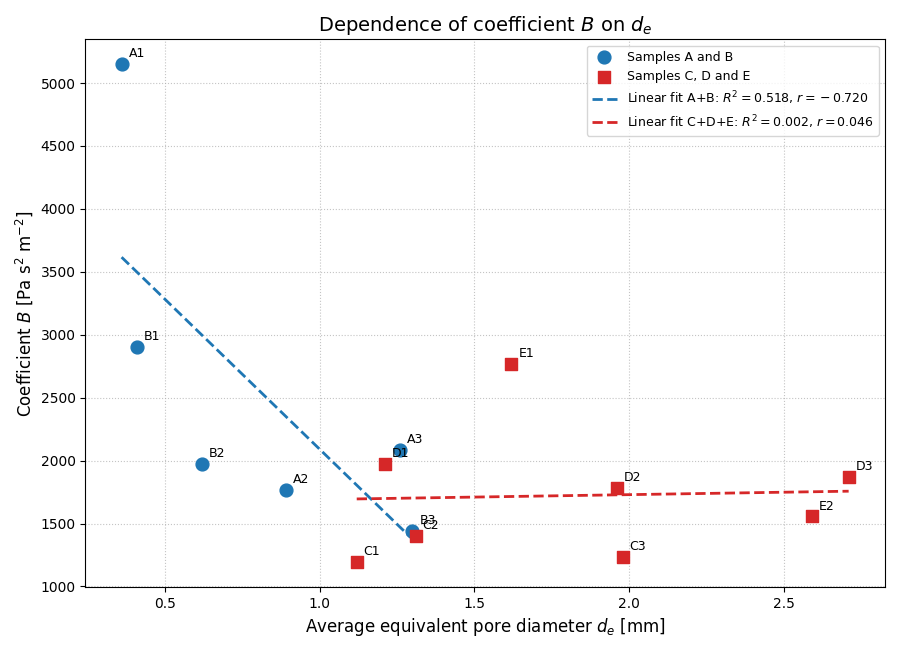
\includegraphics[width=14cm]{korelace_de.png}
  \centering
  \caption{Dependence of the inertial coefficient $B$ on the average equivalent pore diameter.}
  \label{fig:B_de}
\end{figure}

Figure~\ref{fig:B_de} presents the dependence of the inertial coefficient $B$ on the average equivalent pore diameter. In comparison with porosity, a more pronounced relationship is observed for the metallic foams. Samples with larger pore diameters generally exhibit lower values of coefficient $B$, corresponding to reduced inertial pressure losses. This behaviour agrees with the physical expectation that increasing the characteristic flow passage reduces local acceleration of the fluid and therefore decreases form drag within the porous structure. For the ceramic and polymer foams the correlation is less evident, suggesting that additional geometric characteristics influence the hydraulic response.

Overall, the obtained results demonstrate that neither porosity nor the equivalent pore diameter alone is sufficient to predict the hydraulic characteristics of porous materials across different material classes. Nevertheless, the pore diameter provides a more meaningful descriptor than porosity, particularly for metallic foams. The observed scatter further suggests that the pressure-loss coefficients are governed by a combination of several microstructural parameters rather than by a single quantity. Parameters such as pore connectivity, tortuosity or the characteristic size of pore throats are expected to contribute significantly to the hydraulic behaviour and should therefore be considered in future predictive models.

The presented analysis confirms that optical characterization of the porous microstructure provides valuable information about the hydraulic performance of the investigated materials. Although simple one-parameter correlations remain limited, the observed trends support the hypothesis that microstructural descriptors obtained from microscopy can serve as a basis for predicting the hydraulic behaviour of porous materials before experimental testing.

\newpage

\subsection{Conclusions from experimental study}

\newpage

\section{Numerical study of microCT scanned structures}

This chapter describes the numerical model of flow through porous material scanned by microCT.
The goal of this study is to uncover thermohydraulic behavior of water flowing through porous copper structure.
The numerical model is validated against the experimental data obtained from TEALC experimental loop.
Since the porous copper foams are manufactured by a sintering process, the geometry of the porous structure is highly complex and irregular, but the overall morphology of the foam is comparable and largely independent of the manufacturer.
The differences between individual foams are mainly related to scaling, i.e. the characteristic pore size.
MicroCT scans of the same type of porous copper as used in our measurements were kindly provided by Paola Ranut and Enrico Nobile from the University of Trieste, Italy \cite{Ranut2015}.

\begin{figure}[H]
\centering
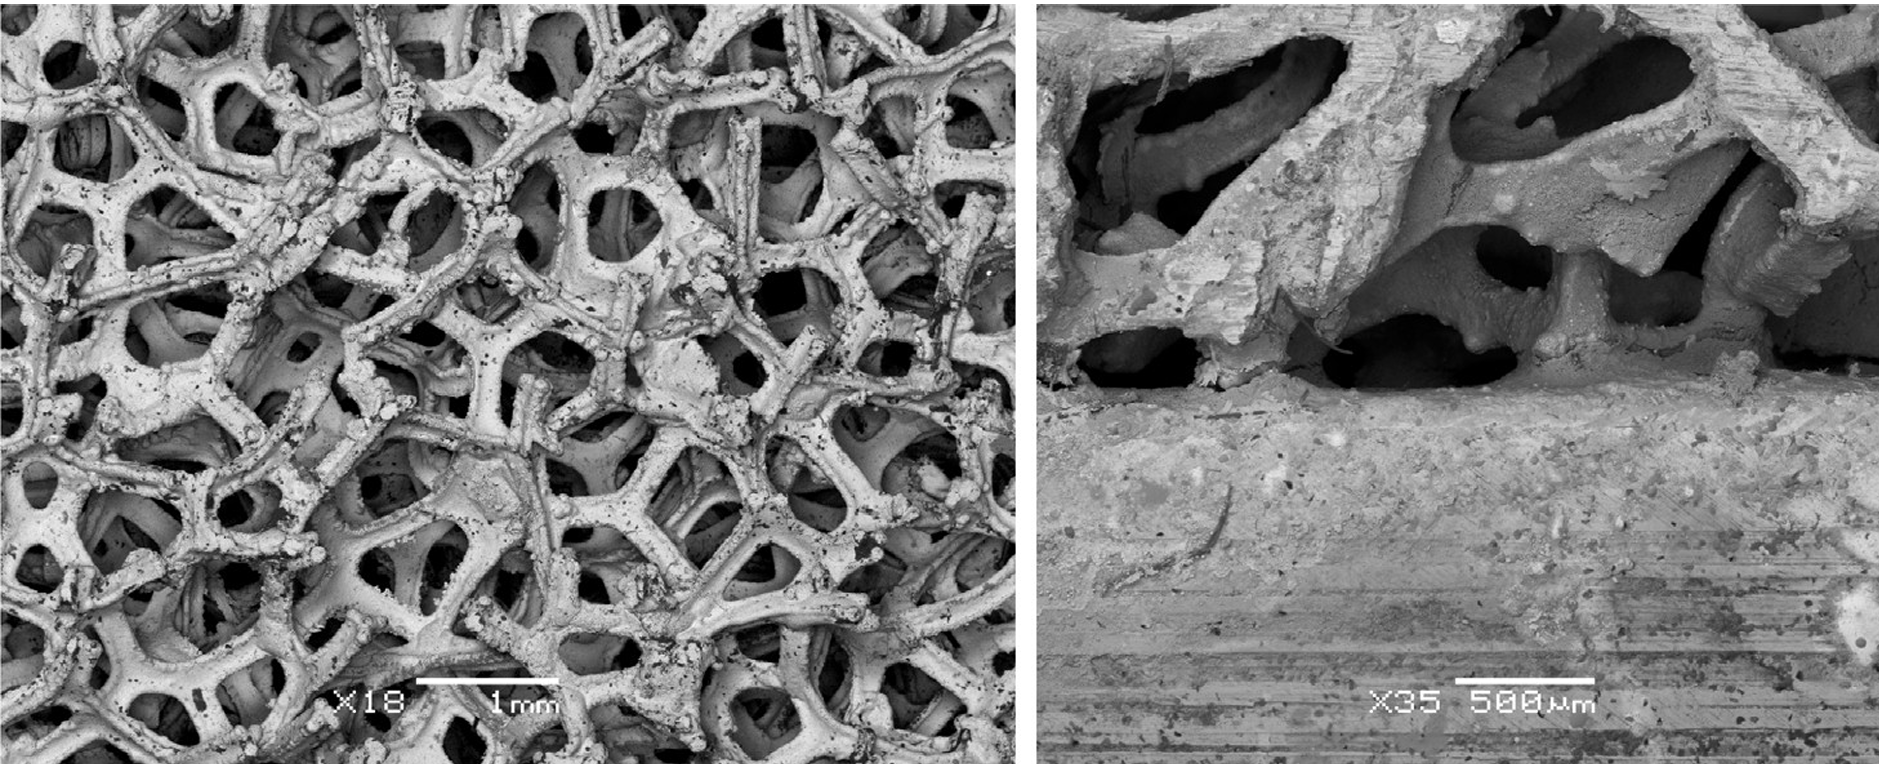
\includegraphics[width=0.8\linewidth]{spojeni_vzorku_exp.png}
\caption{Sample used for the experimental measurements}
\label{fig:exp_samples_spojeni}
\end{figure}

\subsection{Geometry}

The geometry of the porous material is obtained from microCT scans, which provide high-resolution 3D images of the internal structure (Figure \ref{fig:zprac_geom}(a)).
These scans are then processed to create a computational mesh suitable for CFD simulations, shown in Figure \ref{fig:zprac_geom}(b).
Processing of the geometry requires several steps, including noise reduction and smoothing by ShrinkWrap tool in ANSYS SpaceClaim to ensure that the geometry is watertight and suitable for CFD meshing process.
Since the scanned geometry represents only a small portion of the entire sample, it is necessary to extend the geometry by mirroring to ensure the simulated flow in such structure is fully developed.


\begin{figure}[H]
\centering
\begin{subfigure}{0.47\textwidth}
\centering
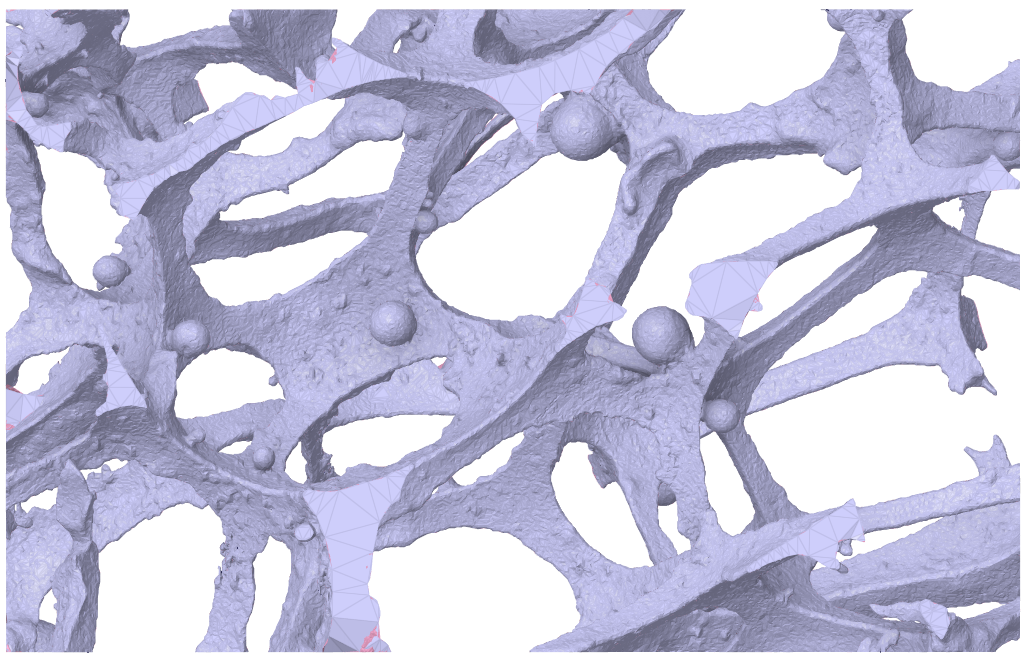
\includegraphics[width=\linewidth]{geometrie_ct_1.png}
\caption{Raw microCT geometry scan}
\end{subfigure}
\hfill
\begin{subfigure}{0.47\textwidth}
\centering
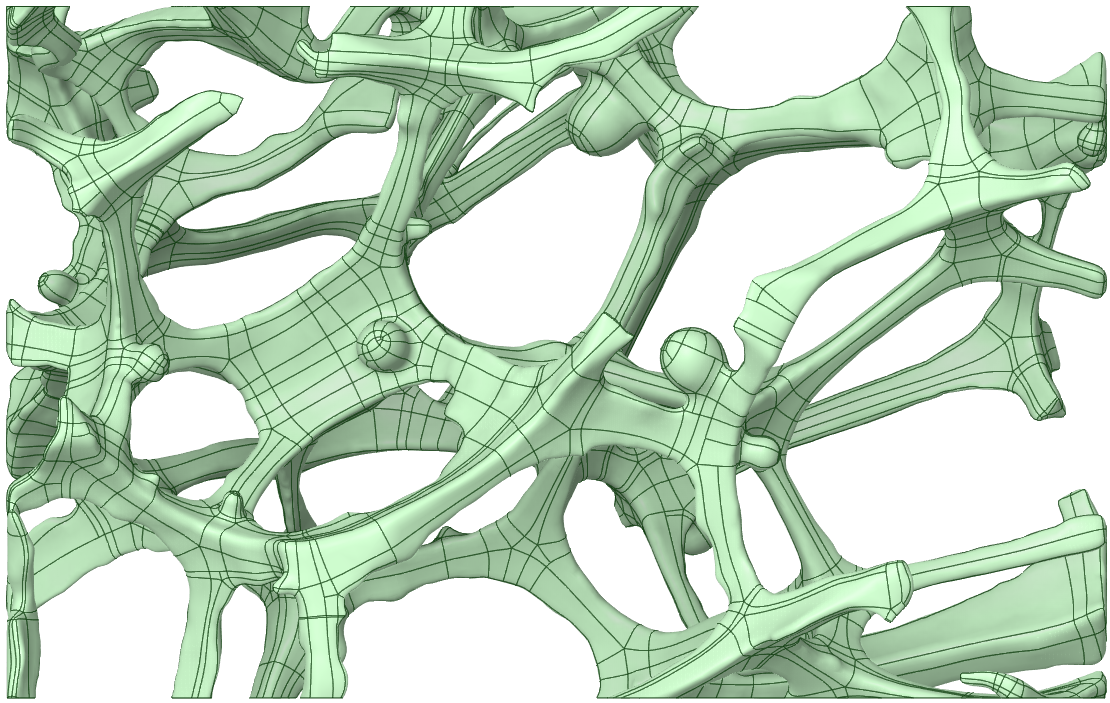
\includegraphics[width=\linewidth]{geometrie_ct_2.png}
\caption{Processed geometry for CFD simulation}
\end{subfigure}
\caption{Porous material samples scanned by microCT}
\label{fig:zprac_geom}
\end{figure}

\pagebreak

Figure \ref{fig:vypoc_geom} shows the CFD domain solved in ANSYS Fluent 2025 R2. 
Inlet and outlet extensions are added to ensure fully developed water flow conditions at the porous structure boundaries.
The porous foam microCT scanned structure is mirrored to increase its volume x4 times, forming a 2~mm long porous section.
Channel wall (WALL\_mid) and porous foam walls (WALL\_foam) are defined as separate boundary conditions to allow separate evaluation of the heat transfer coefficient.

\begin{figure}[H]
\centering
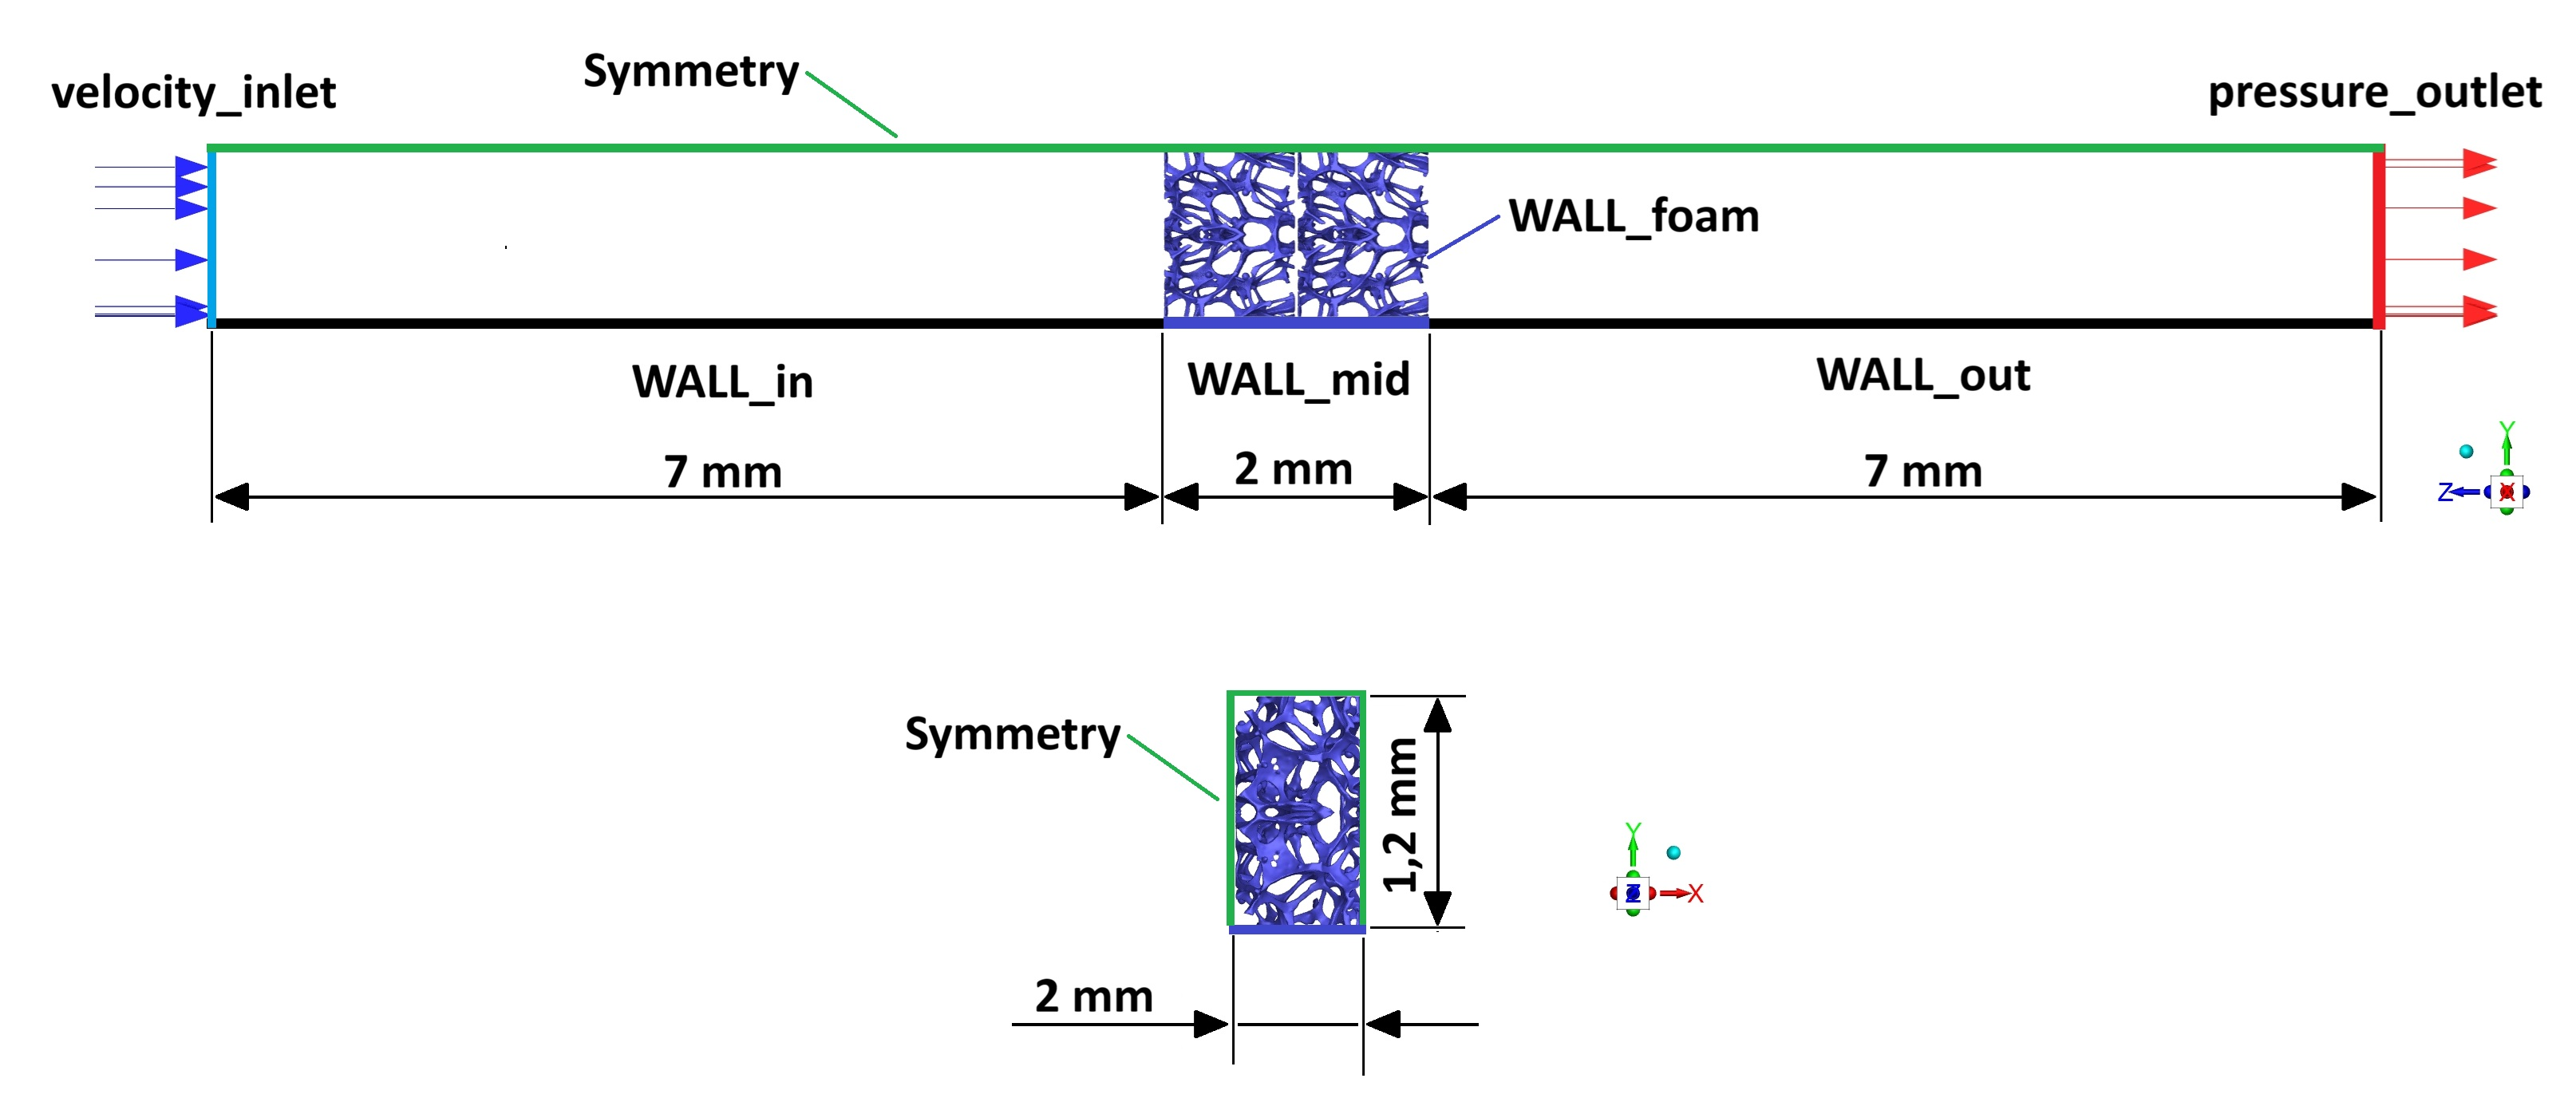
\includegraphics[width=0.98\linewidth]{celek_1.jpg}
\caption{CFD domain solved in ANSYS Fluent 2025 R2}
\label{fig:vypoc_geom}
\end{figure}

\subsection{Mesh sensitivity analysis}

K-omega SST turbulence model is used to capture the flow behavior in the porous structure.
A mesh sensitivity analysis is performed to ensure that the numerical results are independent of the mesh size.
Three different mesh sizes are tested, with the number of mesh cells ranging from approximately 1 million to 2 million.
The mesh sensitivity analysis results are shown in the Figure \ref{fig:mesh_sens}, which plots the pressure drop across the porous structure as a function of the number of mesh cells.

\begin{figure}[H]
\begin{center} % aby byl celý graf na střed strany
\begin{tikzpicture}
\begin{axis}[
    width=12cm,     % kontrola šířky grafu
    height=5cm,     % kontrola výšky grafu
    xlabel={Number of mesh cells $[-]$},
    ylabel={Pressure drop $[Pa]$},
    grid=both,
    ymin=365,
    ymax=380
]

% Čára + body
\addplot[
    color=black,
    mark=*,
    very thick
]
table {
    x y
    1043982 367
    1321924 376
    2012383 377
};

\addplot[
    only marks,
    mark=o,
    mark size=4pt,
    very thick,
    color=red
]
coordinates {(1321924,376)}
node[
    anchor=south west,
    font=\small
] {used mesh};

\end{axis}
\end{tikzpicture}
\end{center}
\caption{CFD mesh sensitivity analysis, $v_{inlet} = 0.26 m.s^{-1}$}
\label{fig:mesh_sens}
\end{figure}

Figure \ref{fig:yplus_distribuce} shows the Y+ distribution on the porous foam walls for the chosen mesh size.
Considering the inlet value 0.26 m.s$^{-1}$ is on the lower end of the velocity range, the Y+ values are expected to be mostly below 1 for all the solved cases, indicating that the mesh is sufficiently fine to accurately capture the near-wall flow behavior using the k-omega SST turbulence model.

\pagebreak

\begin{figure}[ht]
\centering
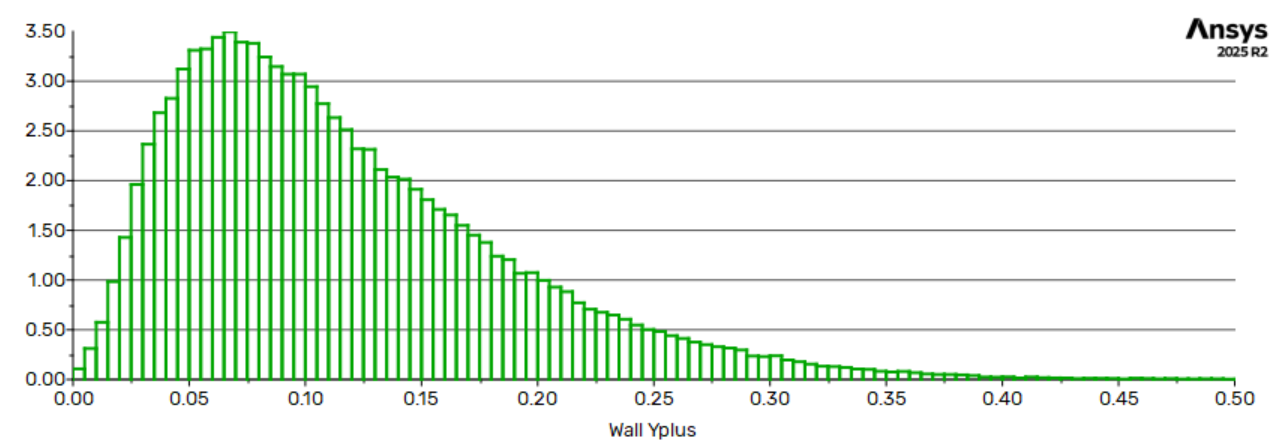
\includegraphics[width=0.98\linewidth]{distribuce_Yplusu.png}
\caption{Y+ distribution on porous foam walls, $v_{inlet} = 0.26 m.s^{-1}$}
\label{fig:yplus_distribuce}
\end{figure}

Figure \ref{fig:line_a} shows the location of Line A, which is used for evaluating the simulation results.
The resulting pressure profile along Line A is shown in Figure \ref{fig:line_a_dp}, demonstrating the pressure drop across the porous structure at an inlet velocity of 0.26 m.s$^{-1}$.

\begin{figure}[H]
\centering
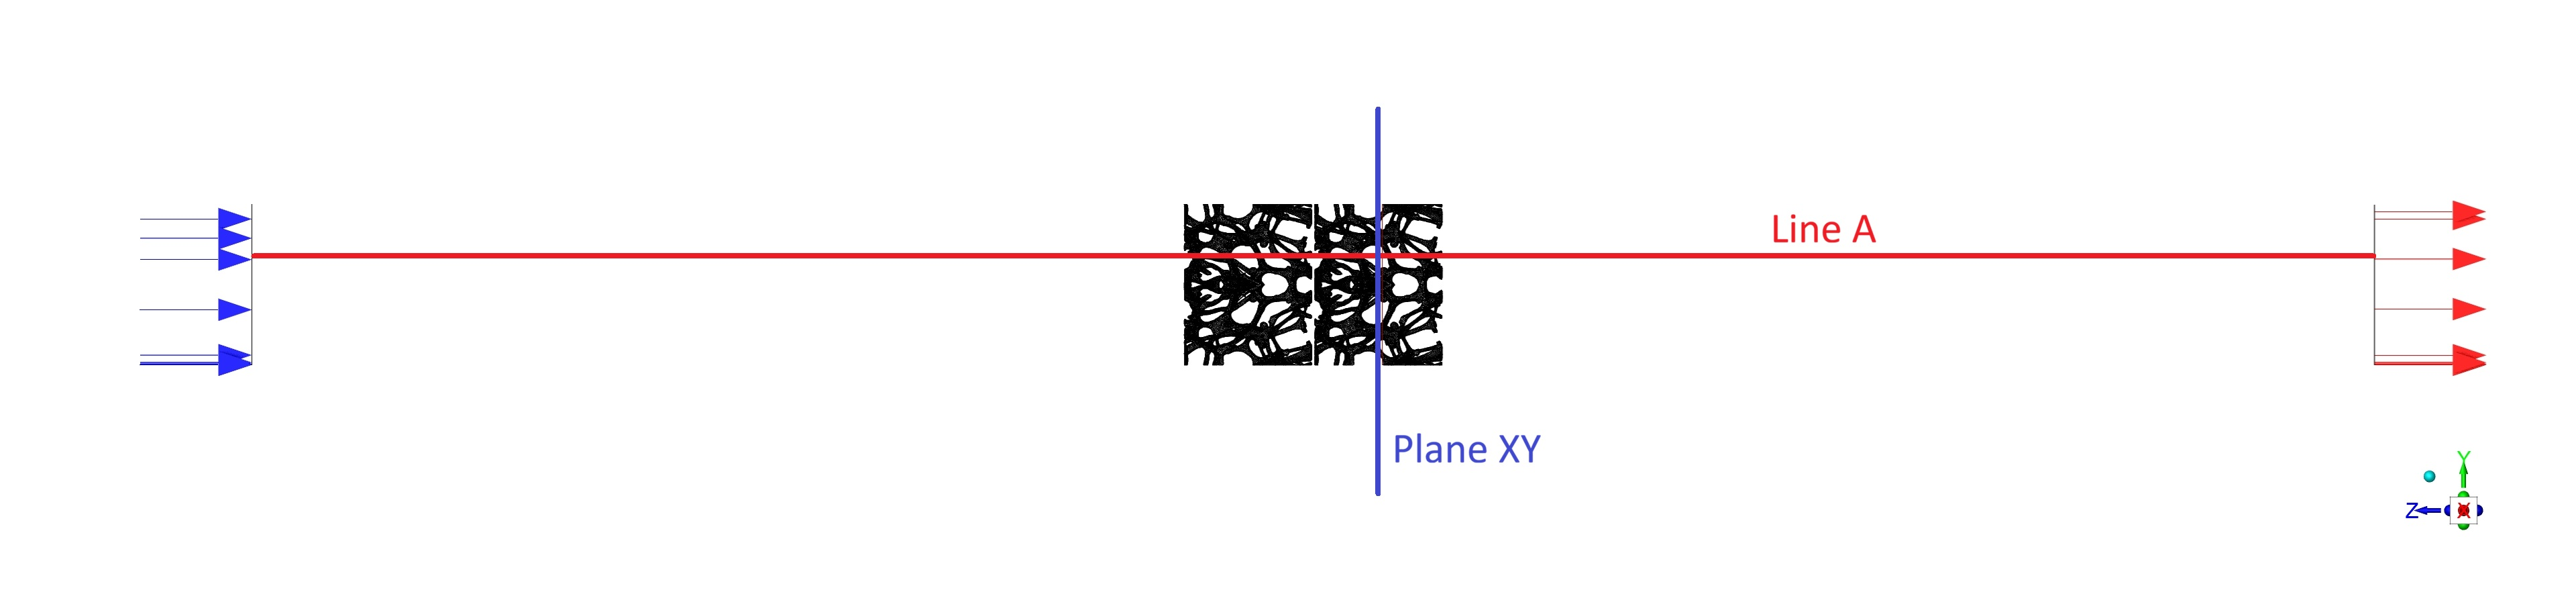
\includegraphics[width=0.98\linewidth]{celek_2.jpg}
\caption{Line A used for result evaluation}
\label{fig:line_a}
\end{figure}

Figure \ref{fig:line_a_dp} shows the flow inside the porous structure is fully developed, with a minimal disturbance at the beginning and the end of porous zone and a linear pressure drop observed across the porous section.
Based on this observation, the pressure drop between inlet and outlet divided by the porous zone length can be used for evaluation of the $dp/dl$ $[Pa/m]$ characteristic.


\begin{figure}[H]
\centering
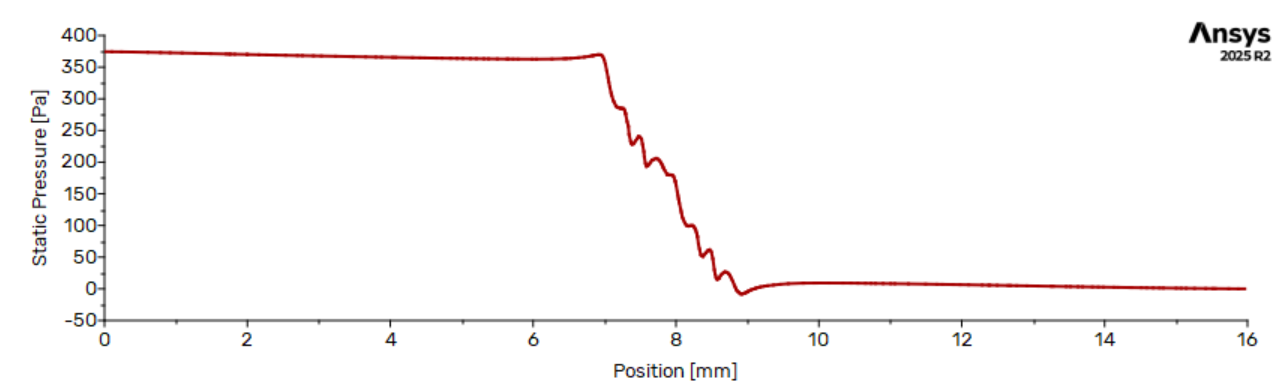
\includegraphics[width=0.98\linewidth]{graf_DP_vzorku.png}
\caption{Pressure profile along Line A, $v_{inlet}=0.26 m.s^{-1}$}
\label{fig:line_a_dp}
\end{figure}


\subsection{Validation - pressure drop}

In order to validate the numerical model, the pressure drop across the porous structure is compared with previously published experimental data \cite{Smolk2024}.
Figure \ref{fig:line_a_dp_validation} shows the comparison of pressure drop per unit length ($dp/dl$) between the numerical and experimental results.
The error rate between the numerical and experimental results is approximately 17~\%.

\begin{figure}[H]
\begin{center} % aby byl celý graf na střed strany
\begin{tikzpicture}
\begin{axis}[
    width=12cm,     % kontrola šířky grafu
    height=8cm,     % kontrola výšky grafu
    ylabel={dp/l $[kPa/m] $},
    xlabel={Flow velocity $[m/s]$},
    xmax=1.2,
    grid=both,
    legend style={
        at={(0.02,0.98)}, % vlevo nahoře uvnitř grafu
        anchor=north west,
        draw=black,
        fill=white,
    }
]

% Čára + body
\addplot[
    color=blue,
    mark=*,
    thick
]
table {
    x y
    0 0
    0.21701 250
    0.43403 583
    0.65104 1000
    0.86805 1580
    1.08507 2333
    1.30208 3166
};
\addlegendentry{Experimental data}

% Další série (příklad)
\addplot[
    color=red,
    ultra thick,
    dashed,
    mark=none
]
table {
    x y
    0 0
    0.21701 144
    0.43403 407
    0.65104 770
    0.86805 1227
    1.08507 1778
    1.30208 2420
    1.5191 3143
    1.73611 3960
    1.95313 4858
};
\addlegendentry{Numerical result}

\end{axis}
\end{tikzpicture}
\end{center}
\caption{Pressure profile along Line A, $v_{inlet}=0.26 m.s^{-1}$}
\label{fig:line_a_dp_validation}
\end{figure}

\subsection{Hydraulic characteristic}

Figures \ref{fig:dp_xy}, \ref{fig:pathlines_velocity} and \ref{fig:profil_rychlosti} show the hydraulic characteristics of the flow through the porous structure at an inlet velocity of 0.26 m.s$^{-1}$.
This velocity is selected as it represents the operating flow rate used in the experimental validation of the heat transfer part of the study.
Figure \ref{fig:dp_xy} shows the pressure profile in the YZ plane, illustrating the pressure drop across the porous structure.
Figure \ref{fig:pathlines_velocity} shows the velocity pathlines within the porous structure, highlighting the complex flow patterns and turbulence induced by the porous geometry.

\begin{figure}[H]
\centering
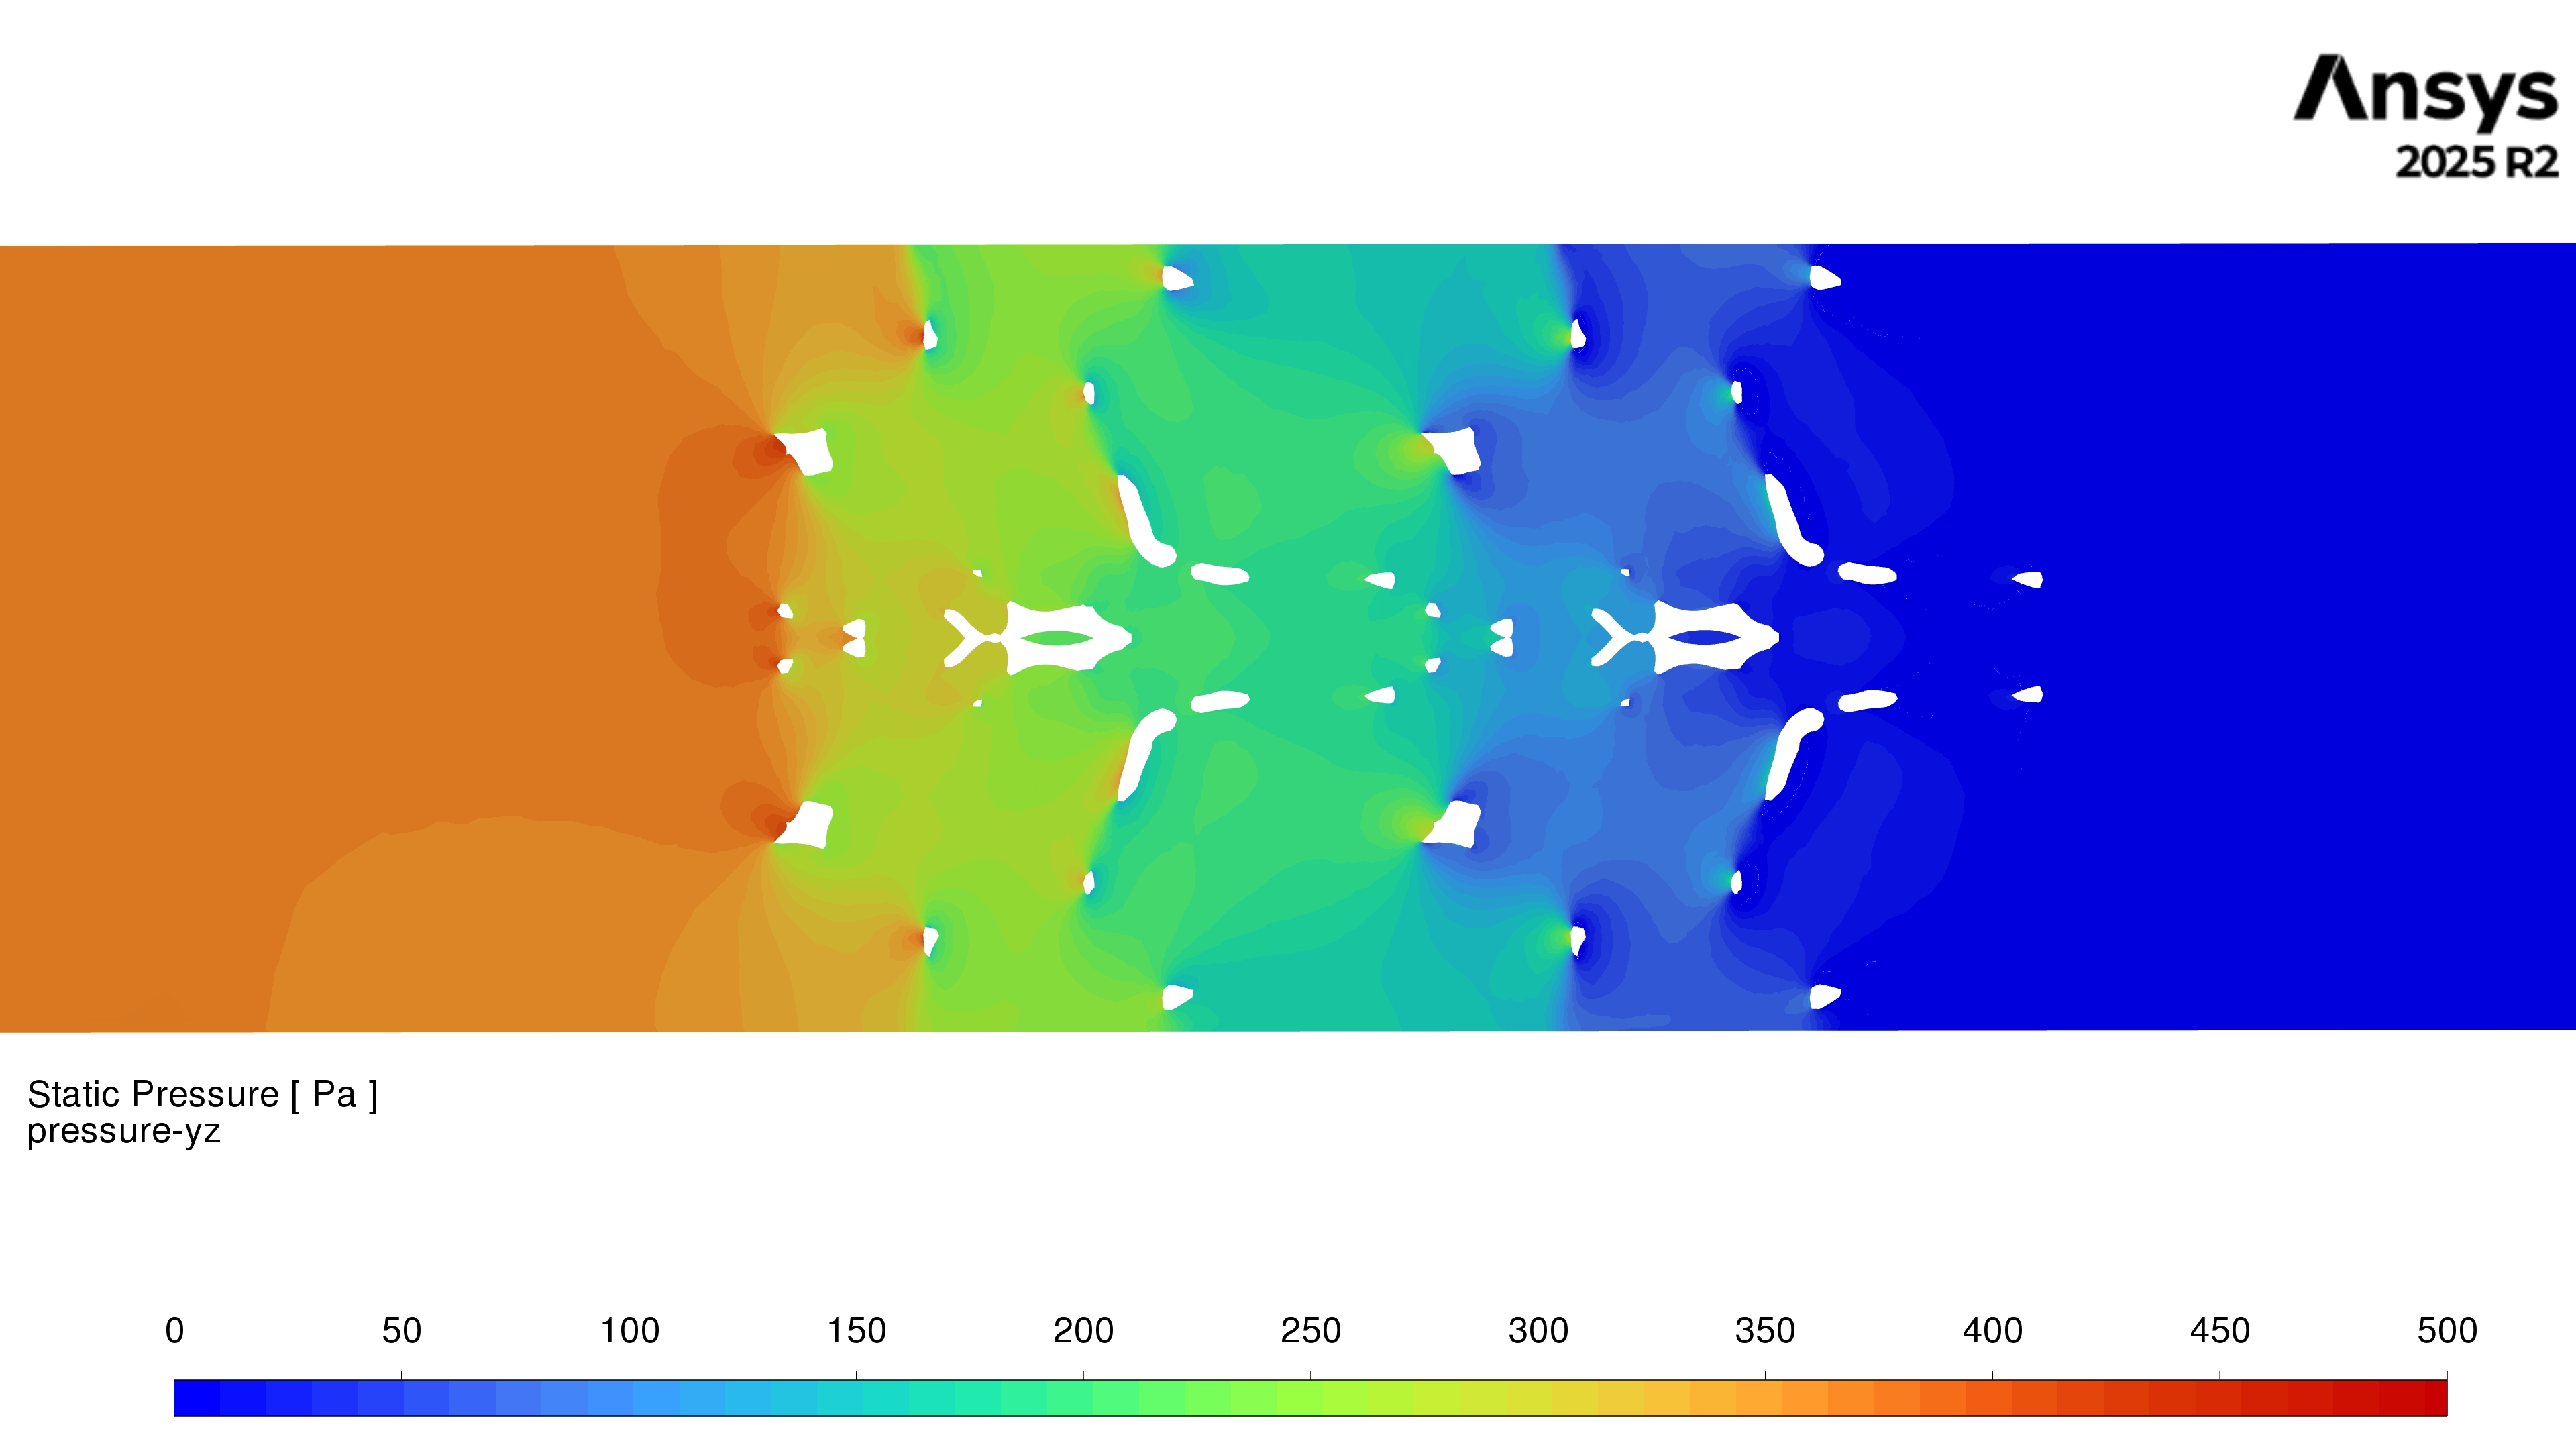
\includegraphics[width=0.98\linewidth]{DPxy.jpg}
\caption{Pressure profile in the YZ plane, $v_{inlet}=0.26 m.s^{-1}$}
\label{fig:dp_xy}
\end{figure}

\begin{figure}[H]
\centering
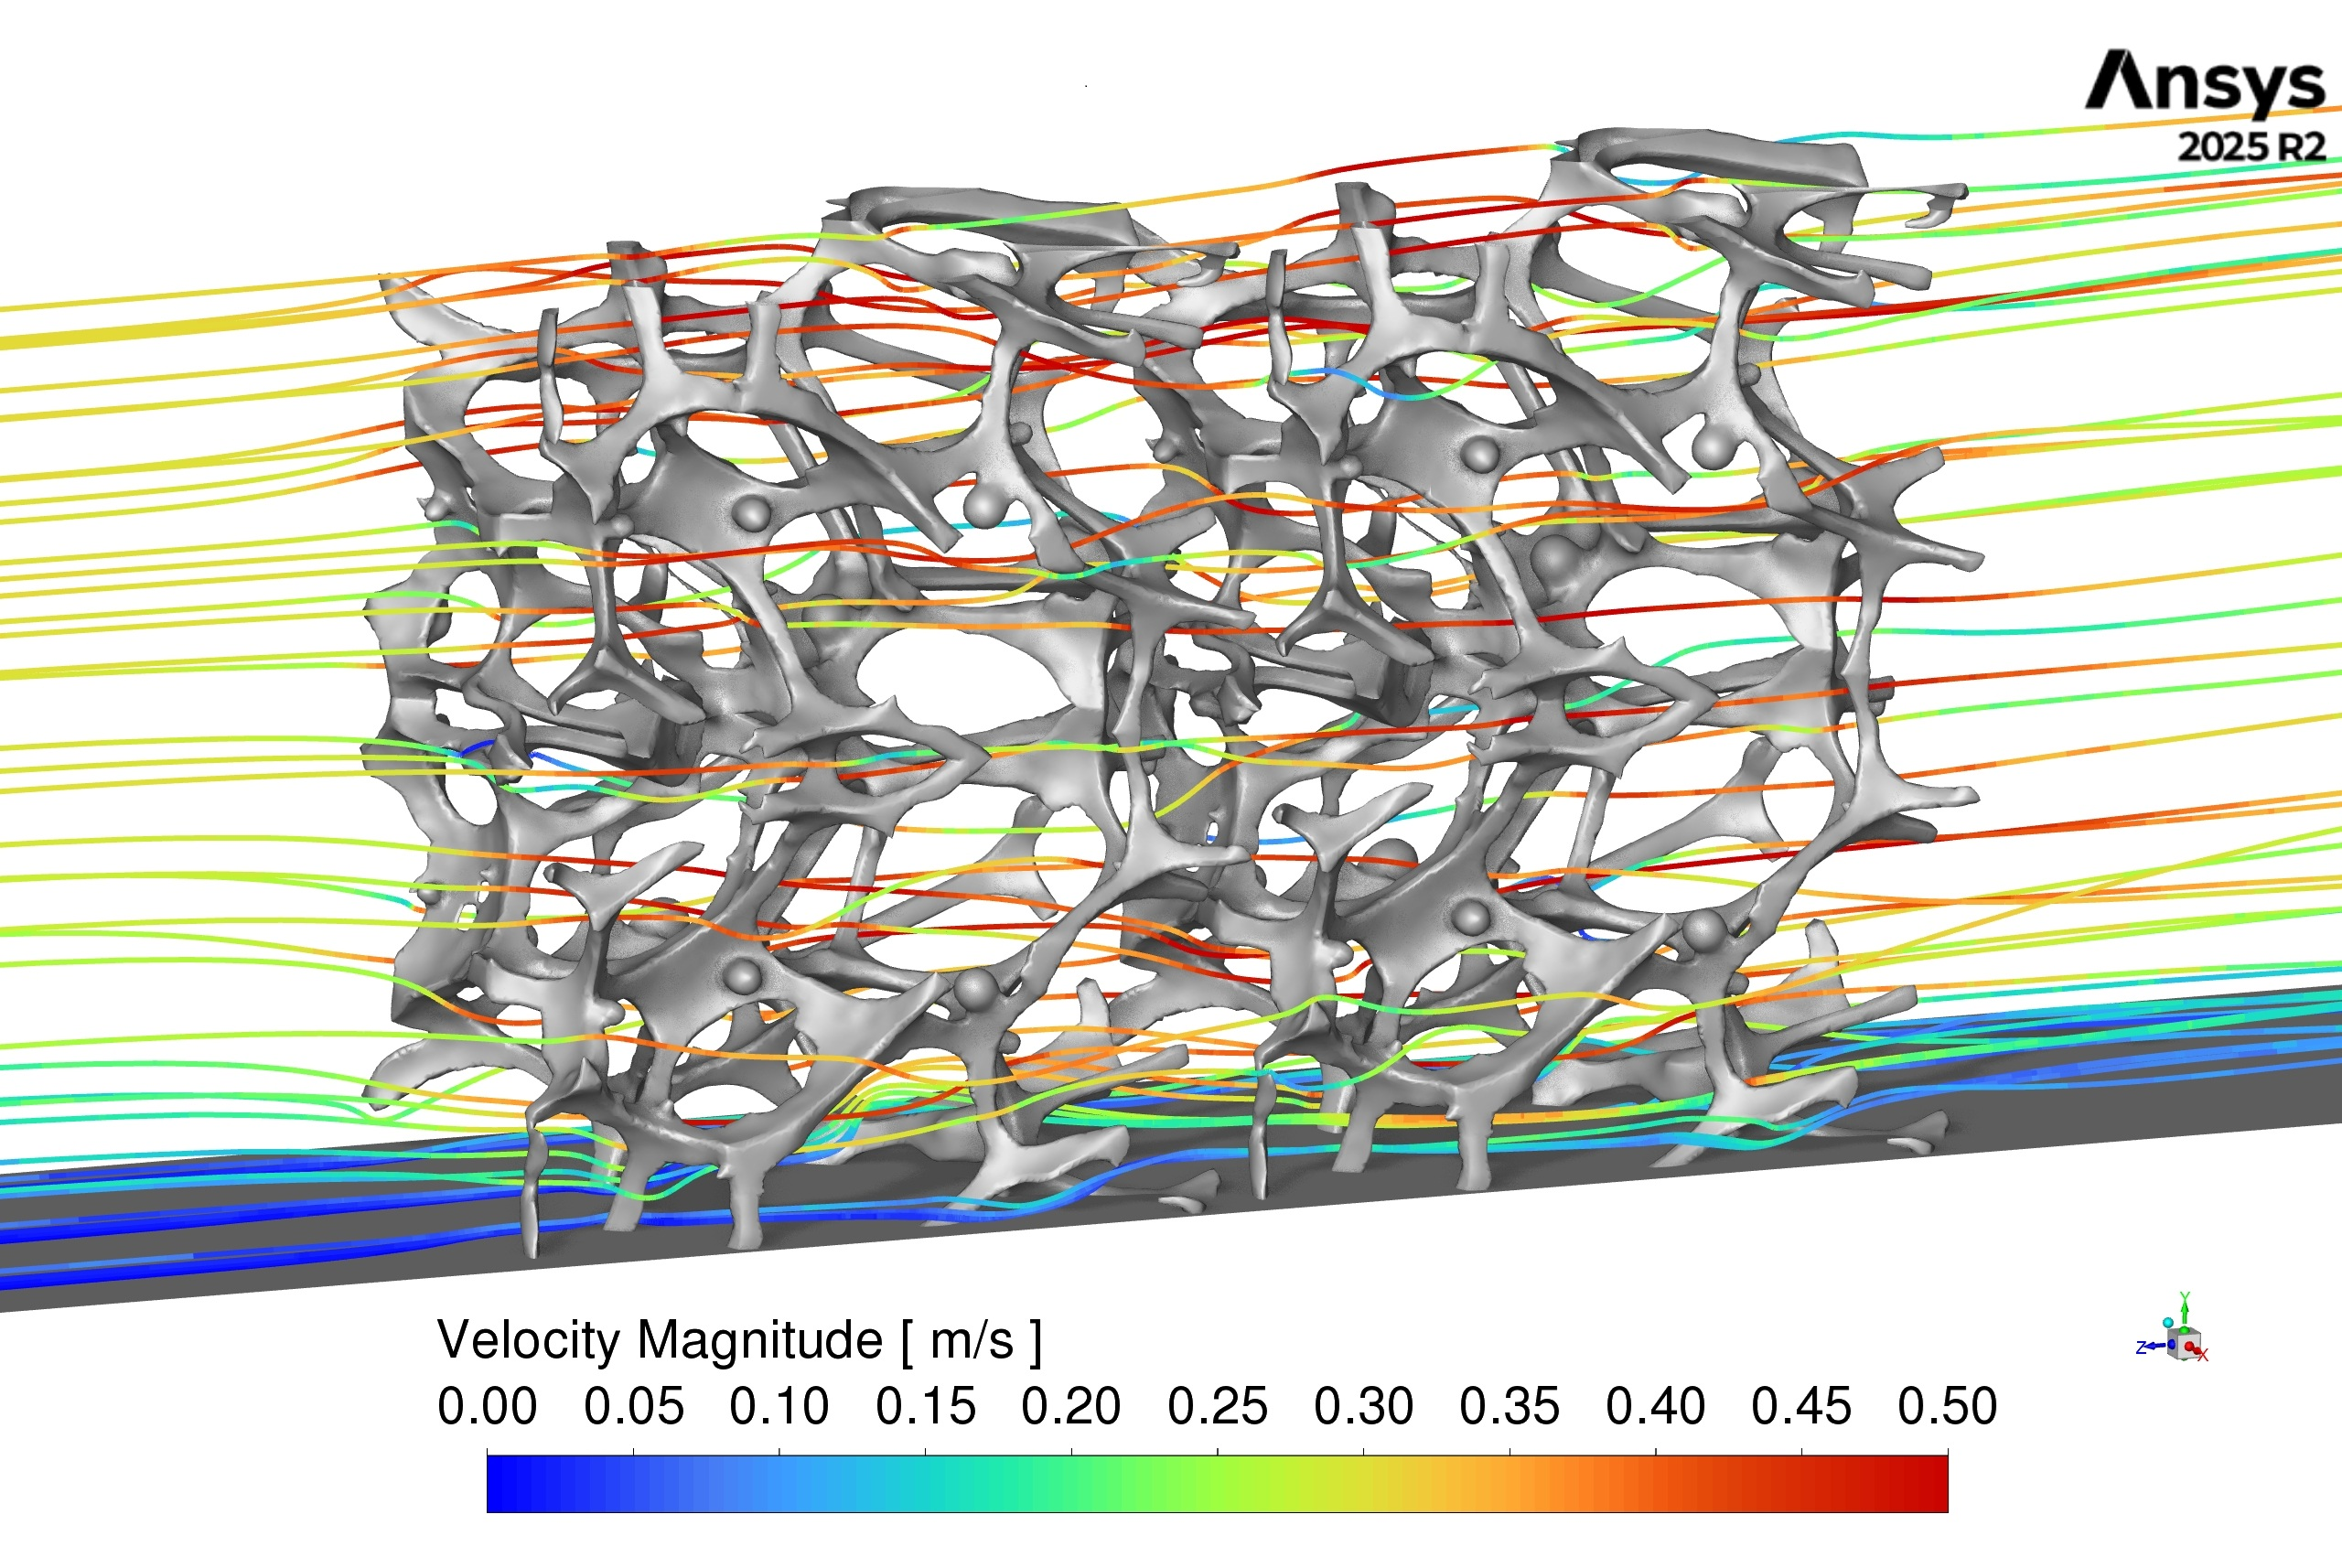
\includegraphics[width=0.98\linewidth]{pathlines_velocity_2.jpg}
\caption{Velocity pathlines in the porous structure, $v_{inlet}=0.26 m.s^{-1}$}
\label{fig:pathlines_velocity}
\end{figure}

Figure \ref{fig:profil_rychlosti} shows the velocity profile along Line A, demonstrating the acceleration and deceleration of the flow as it navigates through the porous medium.
The maximal velocity inside the porous structure reaches up to 2x the inlet velocity due to the complex flow paths within the foam structure.


\begin{figure}[H]
\centering
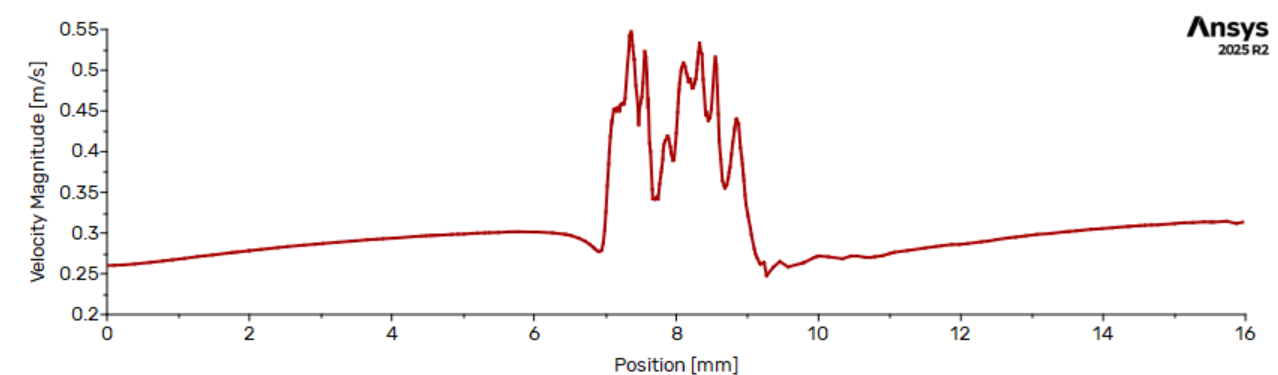
\includegraphics[width=0.98\linewidth]{profil_rychlosti_vzorku.png}
\caption{Velocity profile along the Line A, $v_{inlet}=0.26 m.s^{-1}$}
\label{fig:profil_rychlosti}
\end{figure}


\pagebreak

\subsection{Heat transfer coupled model}

In order to evaluate the heat transfer characteristics of porous materials used in cooling channels, a coupled simulation between ANSYS Fluent and ANSYS Mechanical is employed.
A schematic of the coupled analysis is shown in Figure \ref{fig:flumech_coupled}.
The fluid flow is simulated in ANSYS Fluent, where the heat transfer coefficient at the fluid-solid interface is calculated based on the flow conditions and material properties.
This heat transfer coefficient is then transferred to ANSYS Mechanical as a boundary condition for the thermal analysis of the solid structure.
\\
\\
ANSYS Mechanical is introduced because it provides a robust framework for thermal analysis, especially when dealing with thermal contacts between bodies.
It also provides a possibility to investigate structural changes of the porous structure by both heat expansion and dynamical fluid forces.
Figure \ref{fig:flumech_htc_dist} shows the spatial distribution of the heat transfer coefficient on the foam interface, which is a critical parameter for accurately modeling the thermal behavior of the porous material.
The heat transfer coefficient varies across the interface due to the complex geometry and flow patterns within the porous structure.

\begin{figure}[h!]
    \centering
    \begin{tikzpicture}[
        block/.style={rectangle, draw, minimum width=3cm, minimum height=2cm, align=center, font=\sffamily},
        arrow/.style={-{Stealth[scale=1]}, thick},
        node distance=2cm
    ]

    % Bloky
    \node[block] (fluent) {ANSYS Fluent \\[1mm] Fluid Domain};
    \node[block, right=2cm of fluent] (mechanical) {ANSYS Mechanical \\[1mm] Solid Domain};

    % Horní ohnutá šipka mezi bloky
    \draw[arrow] 
        (fluent.north) 
        .. controls +(1,1) and +(-1,1) .. 
        (mechanical.north) 
        node[midway, above] {Heat transfer coefficient};

    % Vstupní okrajová podmínka vlevo
    \node[left=1cm of fluent] (flow) {Flow velocity};
    \draw[arrow] (flow.east) -- (fluent.west);

    % Vstupní okrajová podmínka nahoře
    \node[above=1cm of mechanical.north east] (inn) {Heat flux load};
    \draw[arrow] (inn.south) -- (mechanical.north east);

    % Výstupní výsledek vpravo
    \node[right=1cm of mechanical] (temp) {Foam Temperature};
    \draw[arrow] (mechanical.east) -- (temp.west);

    \end{tikzpicture}
    \caption{Coupled analysis schematic}
    \label{fig:flumech_coupled}
\end{figure}


Since the heat transfer coefficient is not uniform across the foam interface and it contains local peaks due to the complex geometry and flow patterns, the average value of the heat transfer coefficient is calculated and used as a uniform boundary condition for the thermal analysis in ANSYS Mechanical.

\begin{figure}[H]
\centering
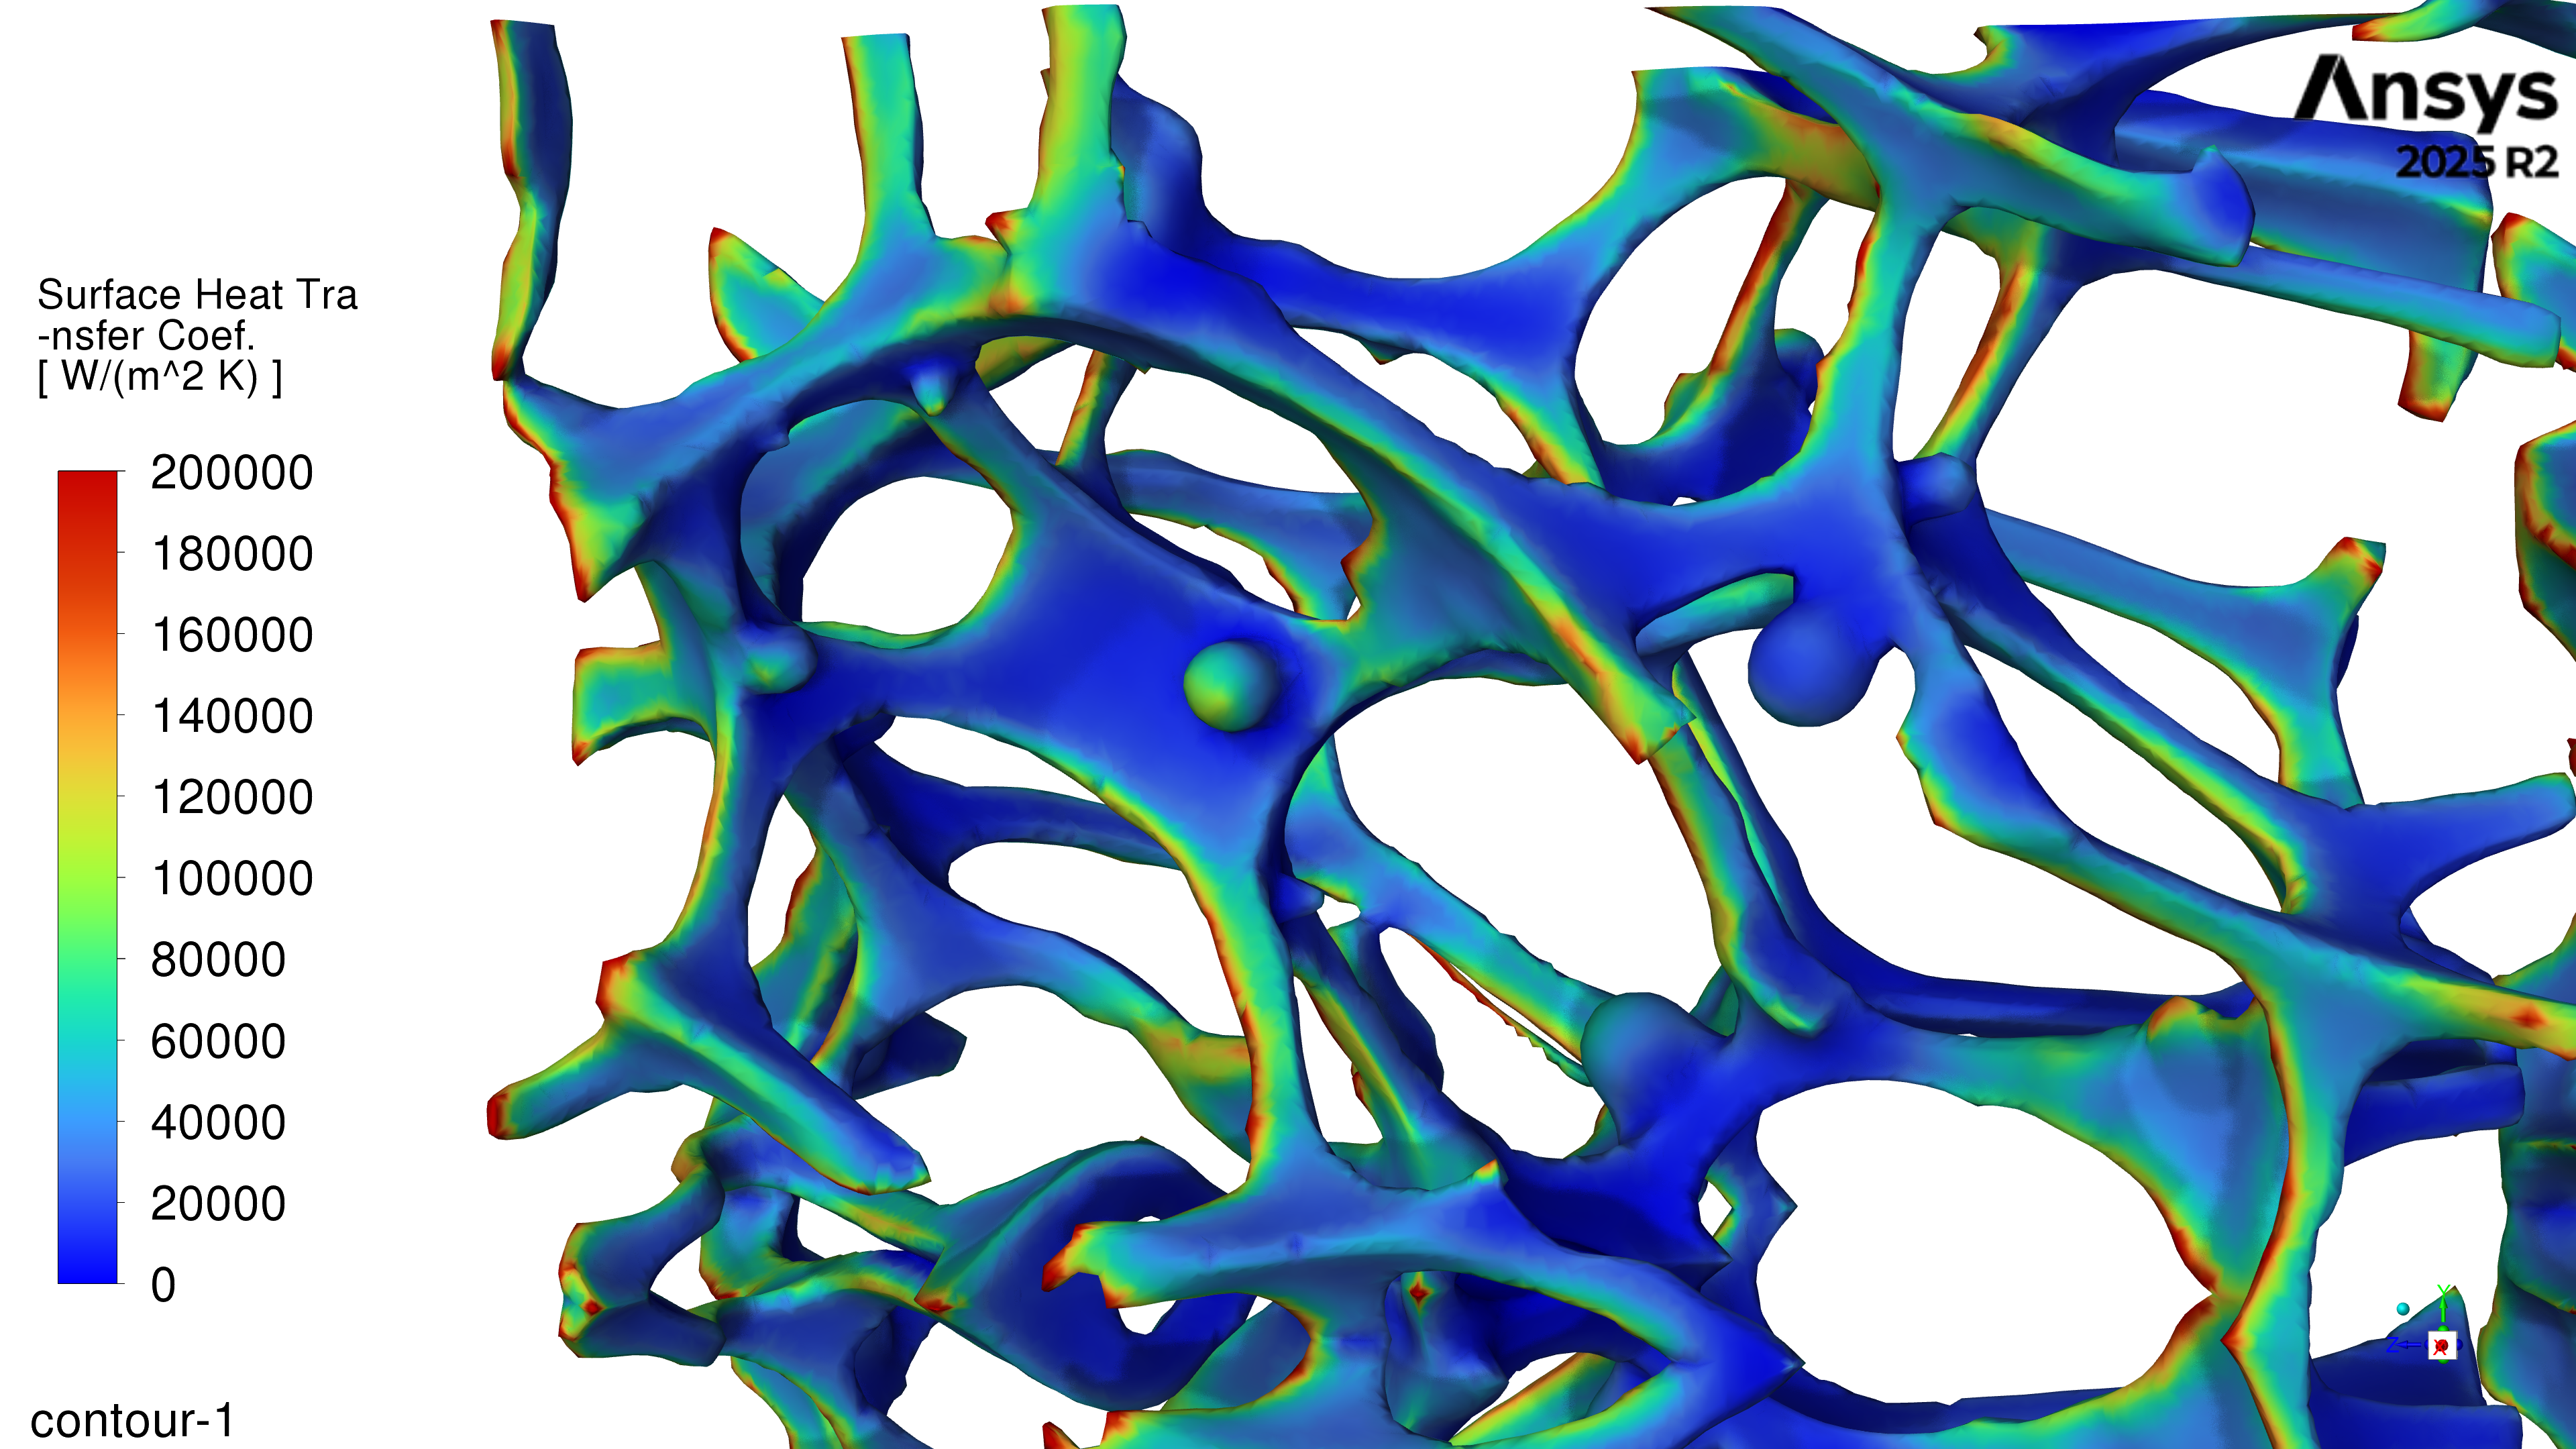
\includegraphics[width=0.9\linewidth]{mfl_7.png}
\caption{Heat transfer coefficient profile on the foam interface, $v_{inlet}=0.26 m.s^{-1}$}
\label{fig:flumech_htc_dist}
\end{figure}

\pagebreak

\begin{figure}[H]
\centering
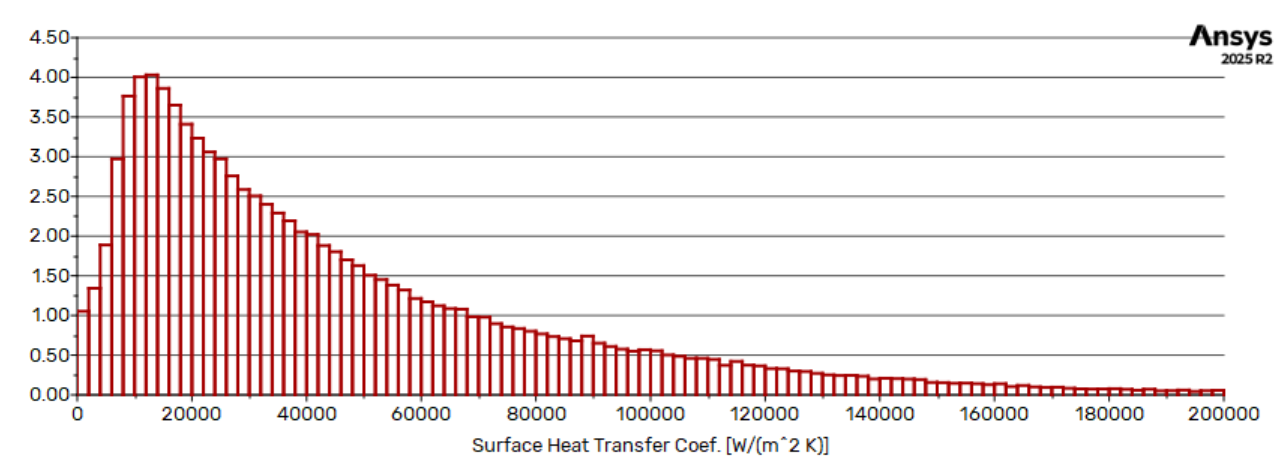
\includegraphics[width=0.9\linewidth]{mfl_1.png}
\caption{Heat transfer coefficient distribution on the WALL\_foam interface, $v_{inlet}=0.26 m.s^{-1}$}
\label{fig:flumech_alpha_dist}
\end{figure}

Area-weighted averaging keeps the total heat flux through the solid-fluid interface consistent, but prevents numerical instabilities in the thermal analysis that could arise from highly localized peaks in the heat transfer coefficient.
Figure \ref{fig:flumech_alpha_dist} shows the distribution of the heat transfer coefficient across the foam interface for the scenario of validation experiment.
In this case, the average value of the heat transfer coefficient is calculated to be 39716 W/m$^2$K, which is then applied as a uniform boundary condition in the thermal analysis of the porous structure in ANSYS Mechanical.
\\
\\
Heat transfer coefficient (HTC) is evaluated separately for the WALL\_mid and WALL\_foam boundary conditions (see Figure \ref{fig:vypoc_geom}), which represent the solid wall and the porous foam interface, respectively.
Since the water flow regime is different near those two walls, the resulting heat transfer coefficient values vary.
Figure \ref{fig:flumech_alpha_dist_v} shows the average heat transfer coefficient on both the foam and the wall interfaces as a function of the inlet flow velocity.
Variable inlet velocity is considered as one of the key parameters influencing the heat transfer coefficient, as it directly affects the flow regime and turbulence characteristics within the porous structure, which in turn impacts the convective heat transfer processes at the fluid-solid interface.
Figure \ref{fig:flumech_alpha_dist_v} illustrates that the heat transfer coefficient on the foam interface (WALL\_foam) is significantly higher than that on the solid wall interface (WALL\_mid) across the entire range of inlet velocities.
The value of HTC for scenario with no porous foam is also included for comparison, showing the effect of the porous structure on enhancing the heat transfer even on the channel wall.


\begin{figure}[H]
\centering
\begin{tikzpicture}
\begin{axis}[
    width=12cm,
    height=7.5cm,
    ylabel={Heat transfer coefficient [$\mathrm{W\,m^{-2}\,K^{-1}}$]},
    xlabel={Flow velocity [$\mathrm{m\,s^{-1}}$]},
    grid=both,
    xmin=0, xmax=1.05,
    ymin=0, ymax=100000,
    legend style={
        at={(0.02,0.98)},
        anchor=north west,
        draw=black,
        fill=white,
        cells={anchor=west},
        align=left
    }
]

% WALL foam
\addplot[
    color=red,
    ultra thick,
    mark=triangle*,
]
table {
    x y
    0.01 3951.7
    0.05 14123.89
    0.1 22124.44
    0.15 28016.64
    0.2 33908.84
    0.25 38797.62
    0.3 43288.81
    0.35 47485.69
    0.4 51456.94
    0.45 55248.98
    0.5 58896.75
    0.6 65845.62
    0.7 72441.39
    0.8 78761.25
    0.9 84860.01
    1.0 90761.77
};
\addlegendentry{WALL\_foam HTC}

% WALL mid
\addplot[
    color=blue,
    ultra thick,
    solid,
    mark=square*,
]
table {
    x y
    0.01 2566
    0.05 4754.24
    0.1 7397.405
    0.15 9319.684
    0.2 11241.96
    0.25 12874.83
    0.3 14376.59
    0.35 15774.07
    0.4 17090.36
    0.45 18345.83
    0.5 19552.31
    0.6 21856.85
    0.7 24061.22
    0.8 26201.1
    0.9 28290.12
    1.0 30321.01
};
\addlegendentry{WALL\_mid HTC}

% WALL mid – no porous foam
\addplot[
    color=blue,
    ultra thick,
    dashed,
    mark=diamond*,
]
table {
    x y
    0.01 2549.5
    0.05 3900
    0.1 5102
    0.15 5795
    0.2 6297
    0.25 6685
    0.3 7008
    0.35 7291
    0.4 7550
    0.45 7796
    0.5 8033
    0.6 8491
    0.7 8951
    0.8 9404
    0.9 9867
    1.0 10319
};
\addlegendentry{WALL\_mid HTC (without the porous foam)}

\end{axis}
\end{tikzpicture}
\caption{Average heat transfer coefficient on the foam and wall interfaces.}
\label{fig:flumech_alpha_dist_v}
\end{figure}


\subsection{Thermal model setup}

Figure \ref{fig:thermal_model_domain}(a) shows the geometry used in the thermal model of solid domain solved in ANSYS Mechanical.
The goal of the numerical model is to evaluate the temperature profiles in the porous foam structure, therefore the geometry was extended in the direction normal to the channel wall to total height of 2.4 mm.
Figure \ref{fig:thermal_model_domain}(b) shows the boundary conditions applied in the thermal model.
Solid wall channel thickness is 2 mm, because the thermocouples used in the experimental validation are positioned 2 mm below the cooled surface.
Heat flux load is applied on the bottom surface, there are two convection boundary conditions defined on the top surfaces: one on the WALL\_mid surface representing the solid wall and one on the WALL\_foam surface representing the porous foam interface.
Heat flux value is set as an input parameter, while the convection boundary conditions use the average heat transfer coefficient values obtained from the ANSYS Fluent analysis.

\begin{figure}[H]
\centering
\begin{subfigure}{0.4\textwidth}
\centering
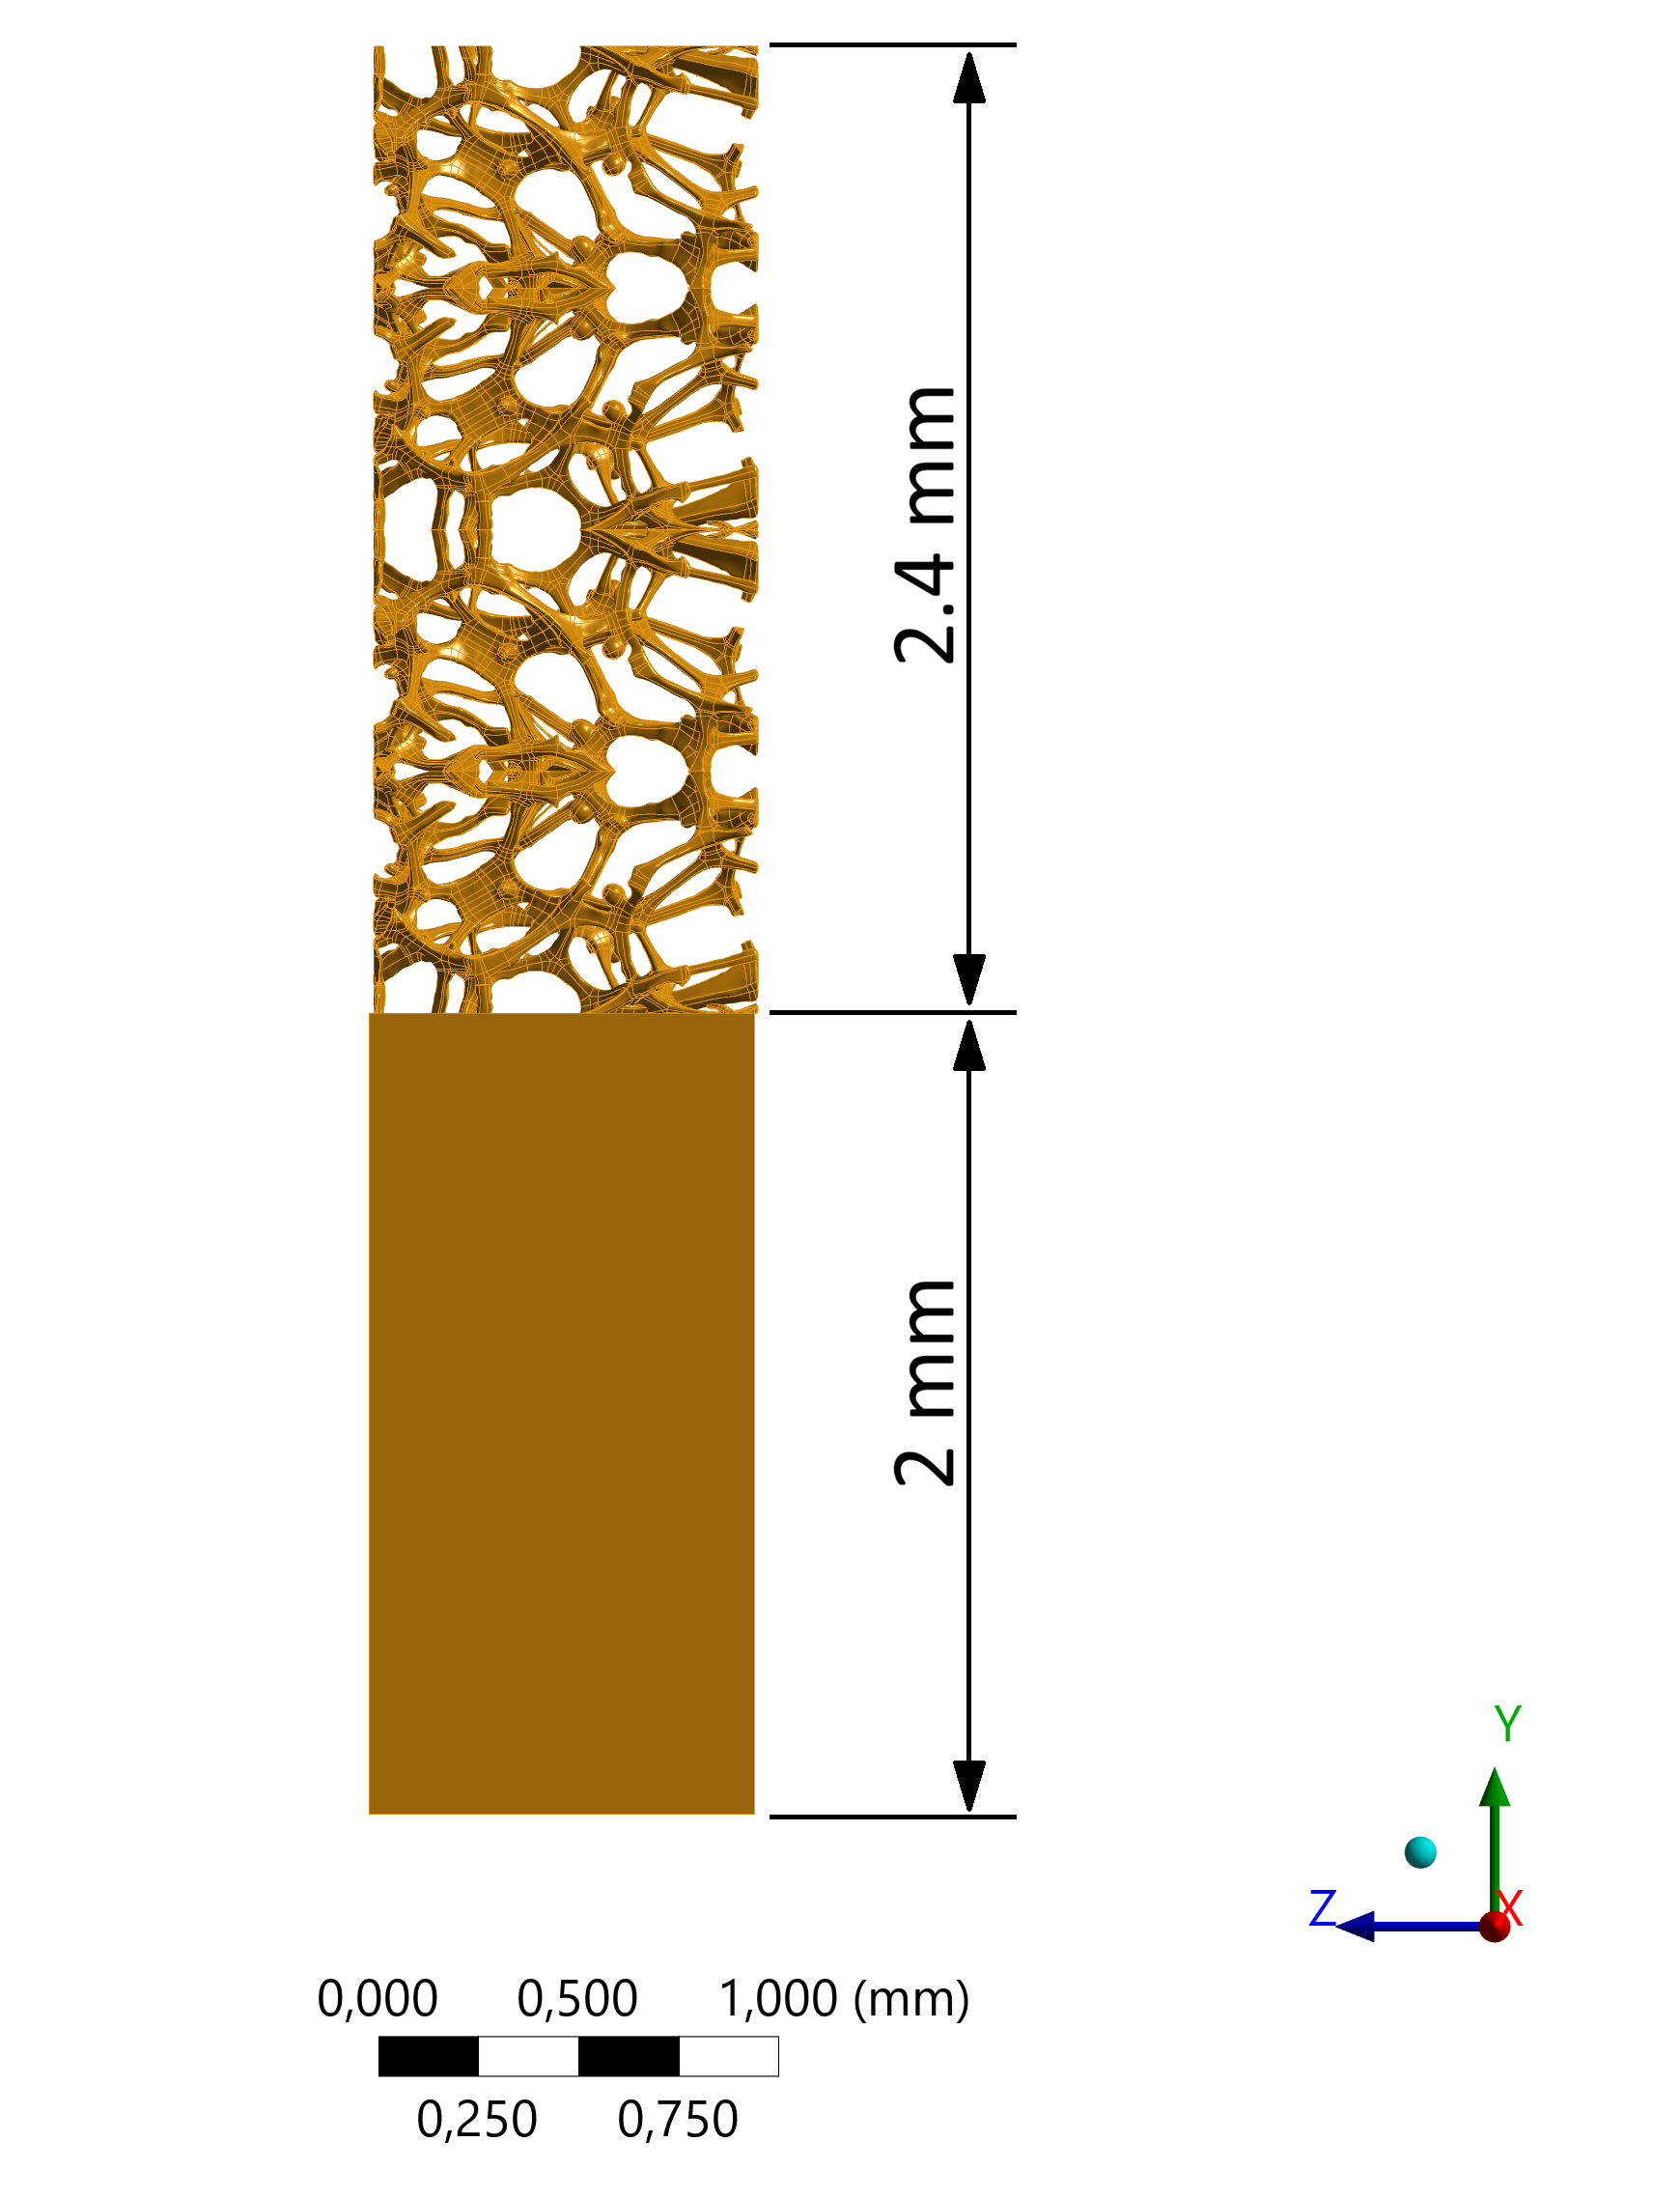
\includegraphics[width=\linewidth]{mfl_6.png}
\caption{Geometry dimensions.}
\end{subfigure}
\hfill
\begin{subfigure}{0.5\textwidth}
\centering
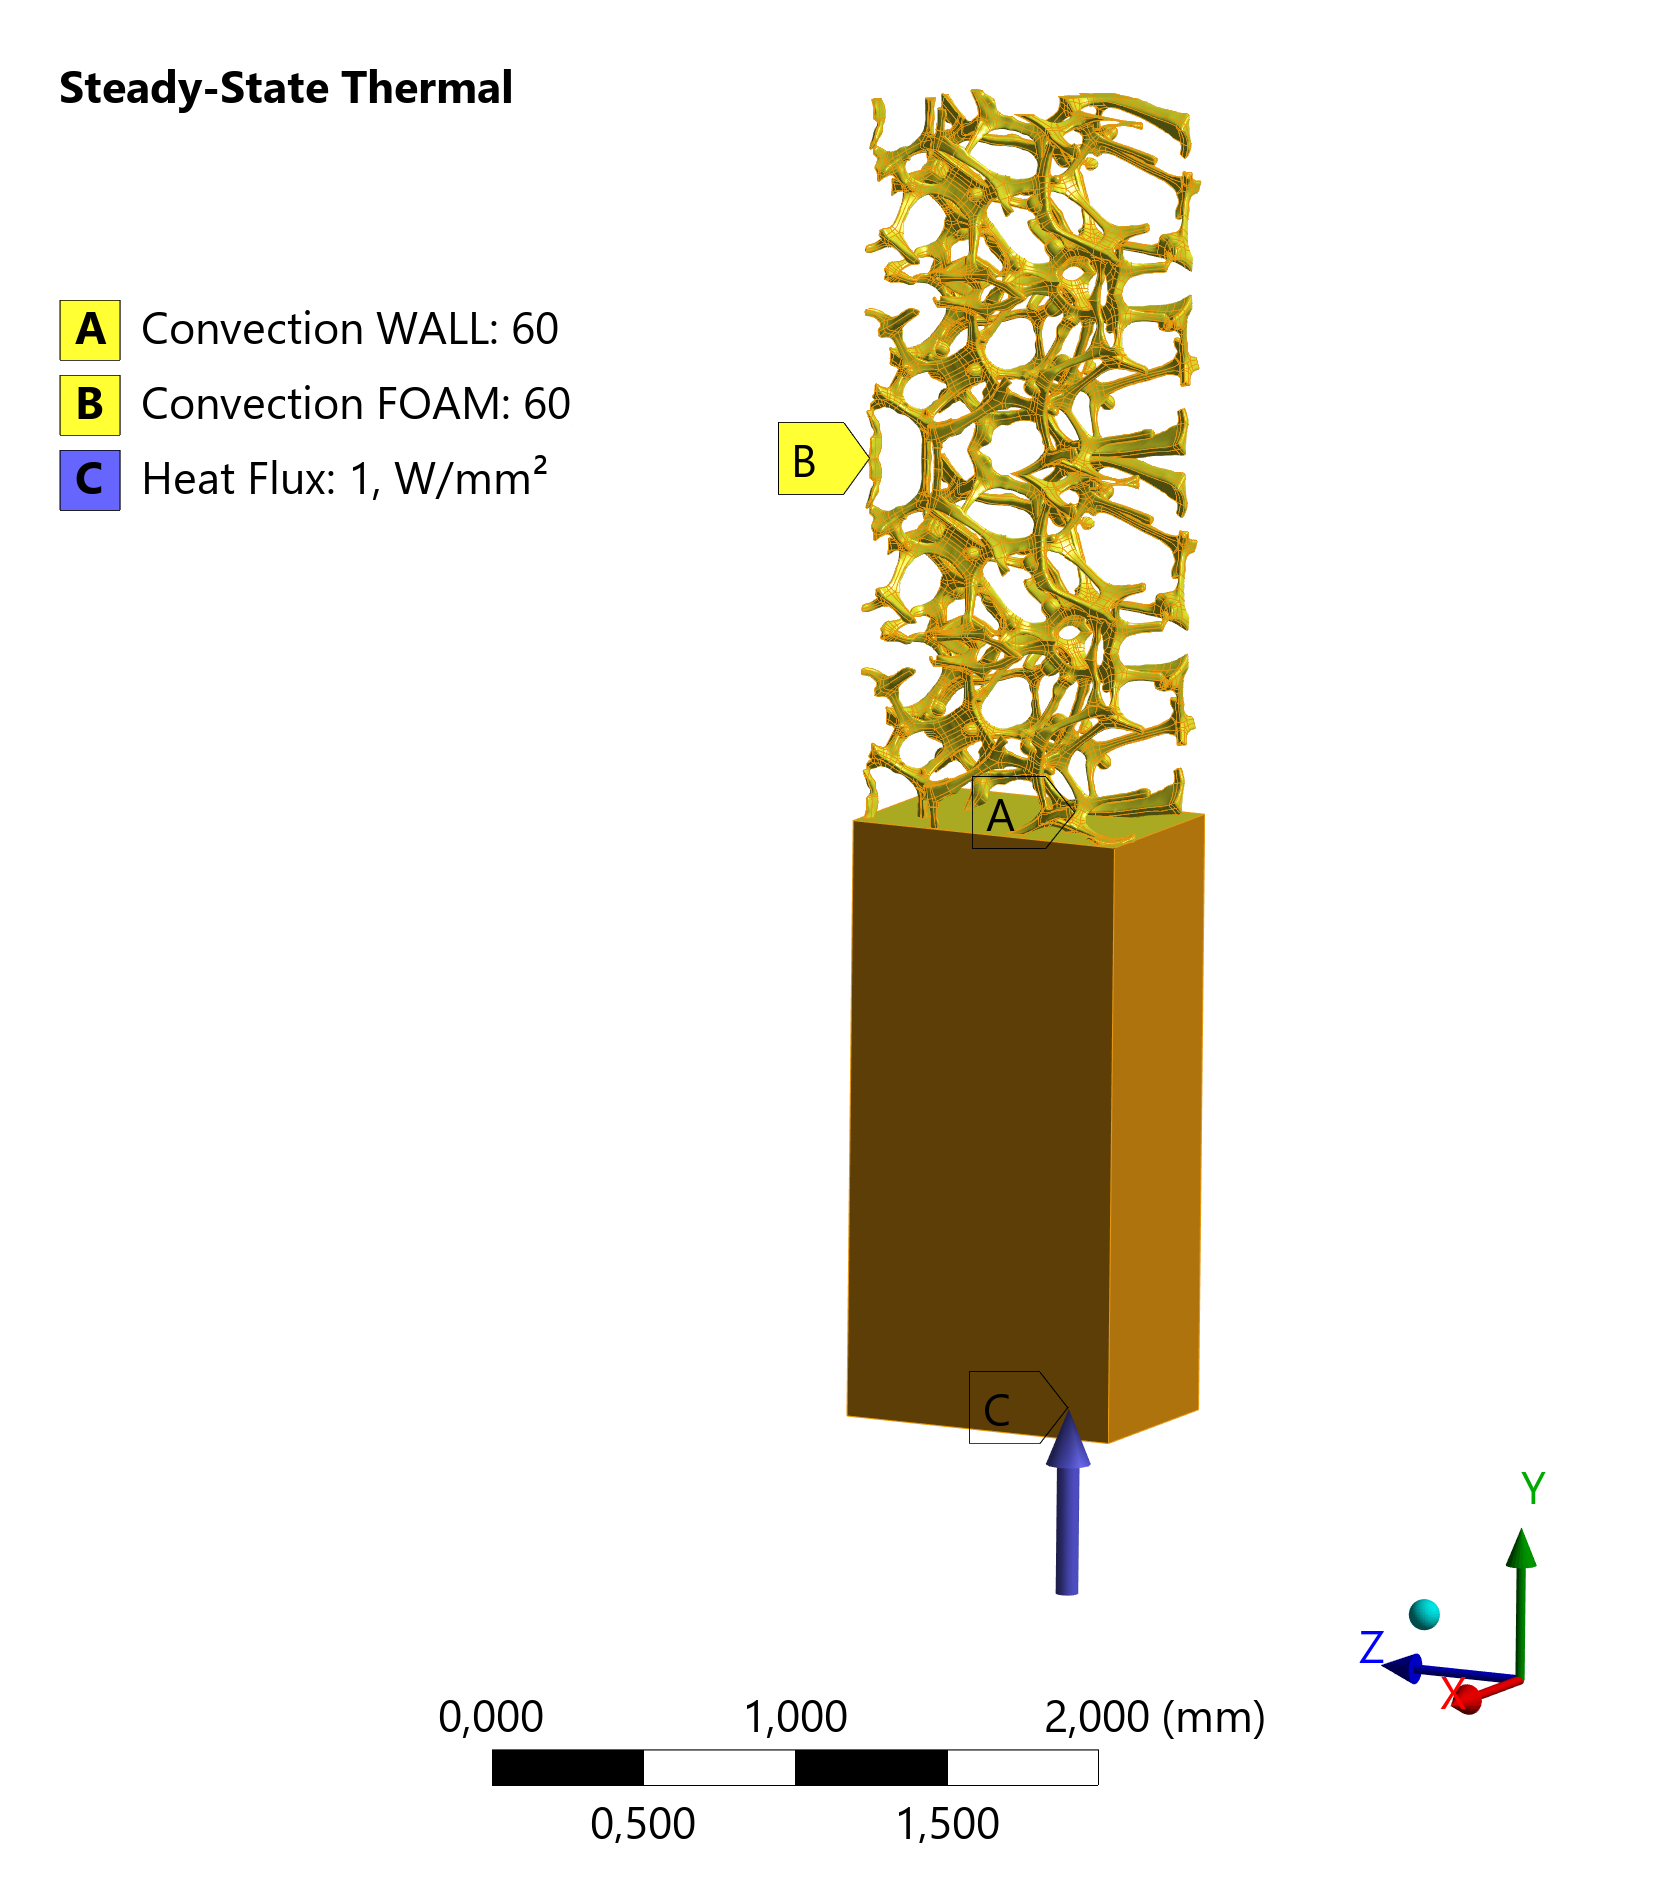
\includegraphics[width=\linewidth]{mfl_5.png}
\caption{Boundary conditions.}
\end{subfigure}
\caption{ANSYS Mechanical thermal model of solid domain.}
\label{fig:thermal_model_domain}
\end{figure}




\subsection{Thermal contacts}


Figure \ref{fig:exp_samples_spojeni} shows microscopy photo of the contact region between the solid wall and the porous structure body.
The connection between these two bodies is a soldered joint (Sn97Cu3 soldering paste), which is characterized by a specific contact conductance.
This contact conductance is defined as the ratio of the thermal conductivity of the contact material ($\lambda_{\text{Sn97Cu3}}$) to the thickness of the contact layer ($t_{\text{soldered}}$), as shown in Equation \ref{eq:contact_conductance}.
According to the Figure \ref{fig:exp_samples_spojeni}, the thickness is estimated to be approximately 0.5 mm, thermal conductivity of Sn97Cu3 soldering paste is expected to be at 50 W/mK, resulting in the contact conductance value of 100 000 W/m$^2$K.
Contact connection between porous foam body and solid wall is shown in Figure \ref{fig:thermal_contact}.
The contact regions on WALL\_mid surface are excluded from the convection boundary condition to prevent double counting of the heat transfer in these areas.

\begin{equation}\label{eq:contact_conductance}
TCC_{\text{contact}} = \frac{\lambda_{\text{Sn97Cu3}}}{t_{\text{soldered}}} = \frac{50 \, W/mK}{0.0005 \, m} = 100000 \, W/m^2K
\end{equation}


\begin{figure}[H]
\centering
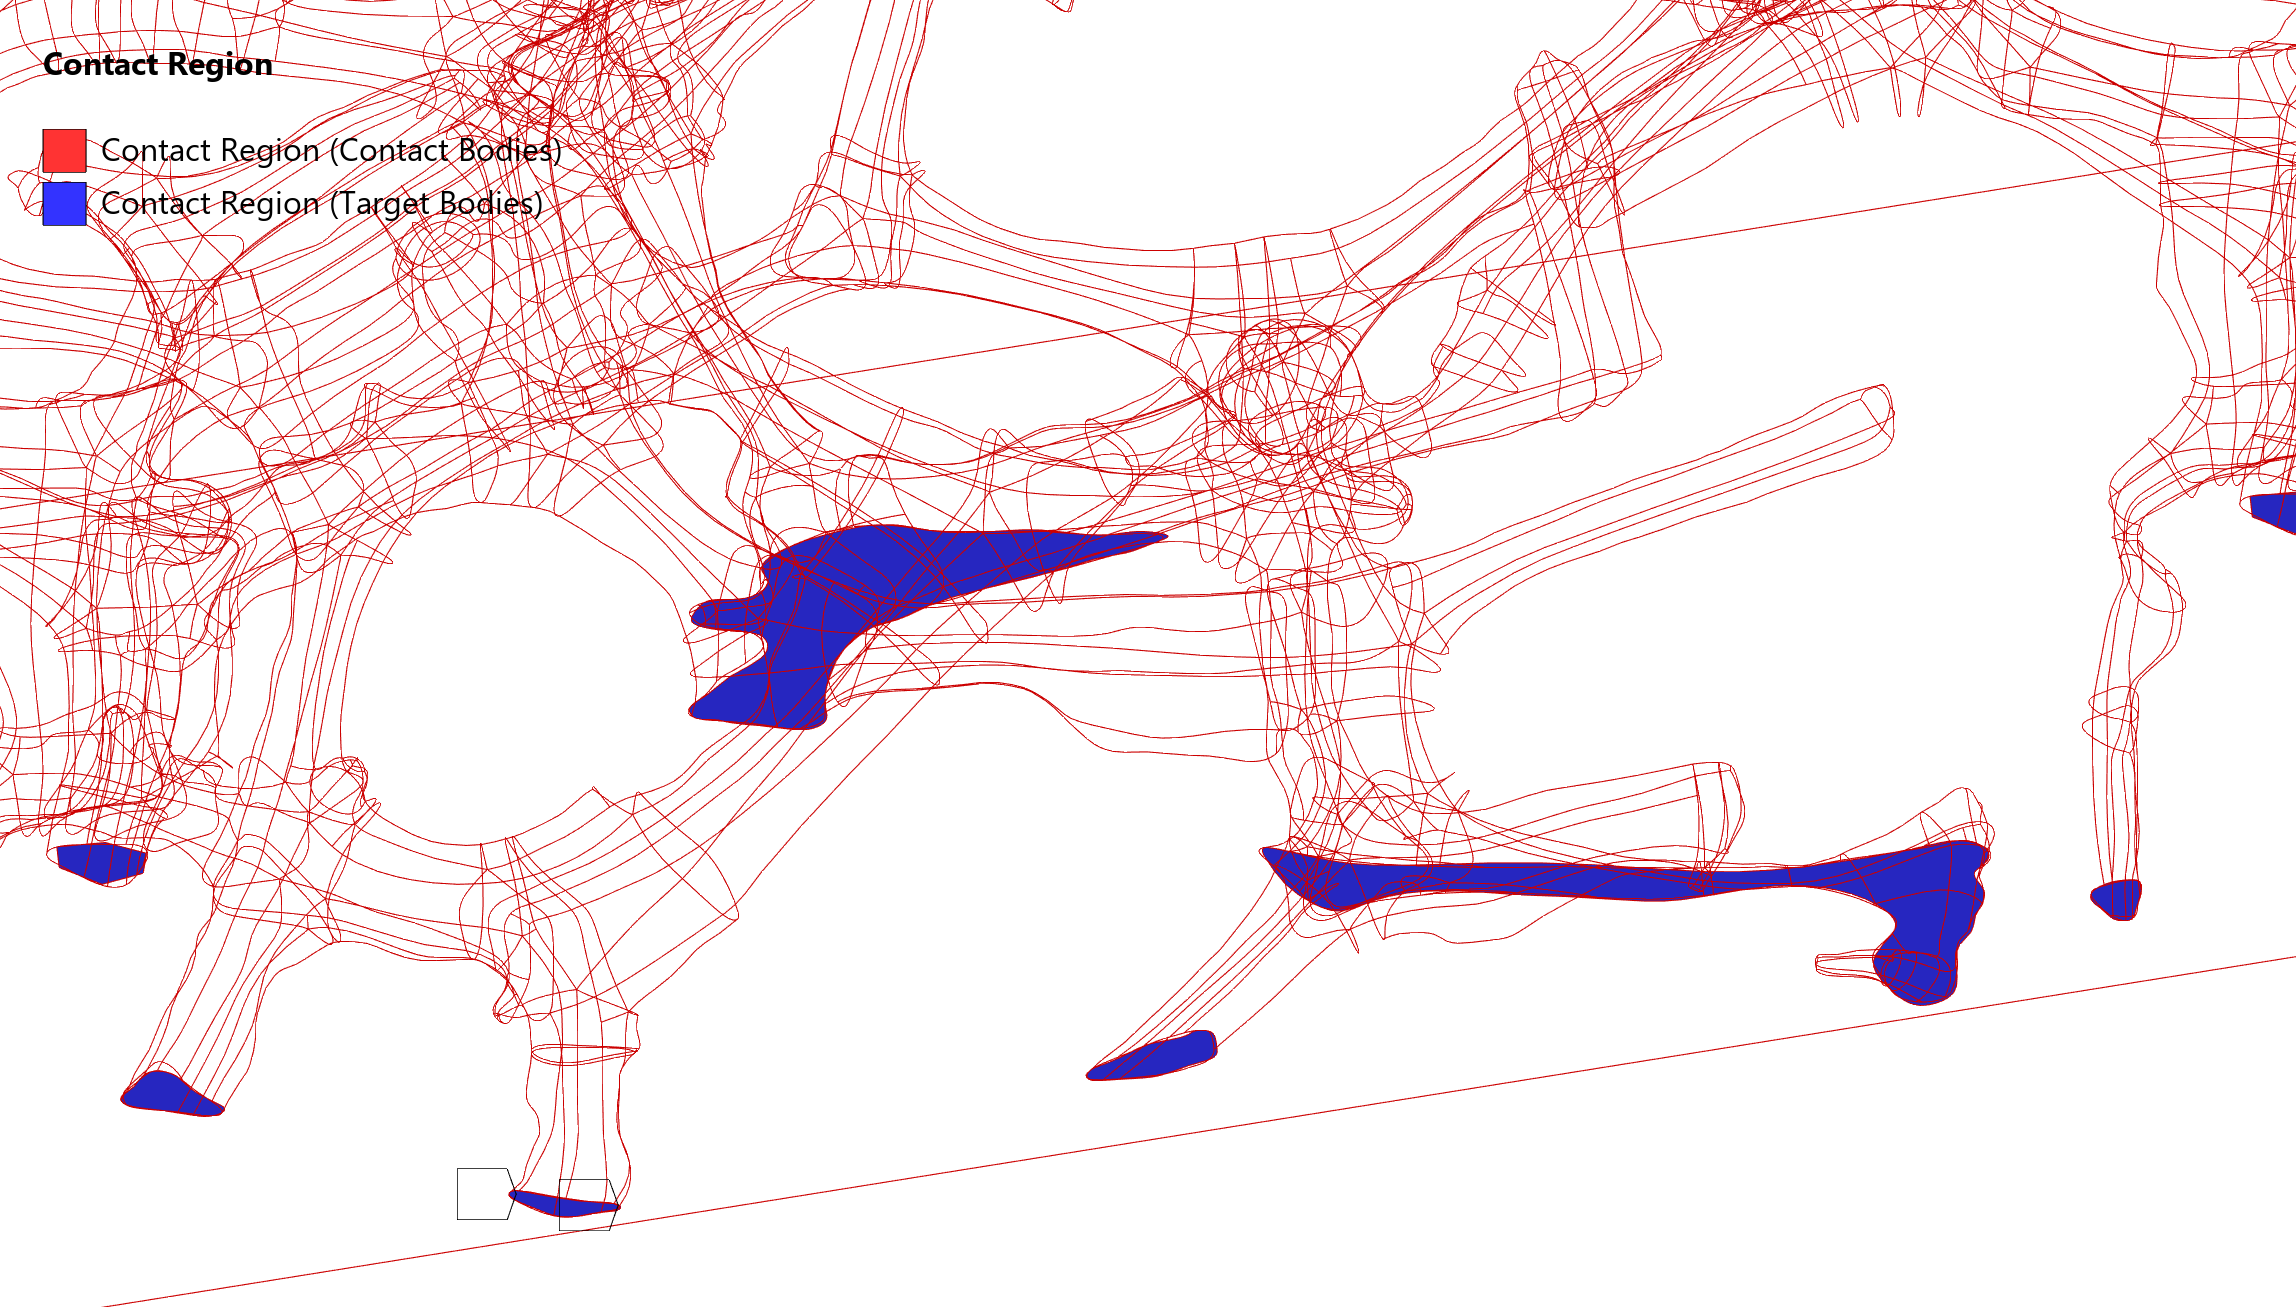
\includegraphics[width=0.8\linewidth]{mfl_4.png}
\caption{Contact regions between WALL\_mid and porous structure body.}
\label{fig:thermal_contact}
\end{figure}


\subsection{Thermal validation}

Figure \ref{fig:validate_thermal_model_x} shows the comparison of thermocouple measurements from the experimental setup with the numerical results obtained from the numerical model.
Resulting temperature was evaluated as the average temperature on the surface where the heat load is applied (bottom surface in Figure \ref{fig:thermal_model_domain}(b)).
The thickness of the solid wall is 2 mm, which corresponds to the position of the thermocouples in the experimental setup.
The error rate between the numerical and experimental results is approximately 6~\%, which indicates a good agreement between the two.
Thermal model is therefore validated and can be used for further analysis of temperature profiles in the porous foam structure.

\begin{figure}[H]
\begin{center} % aby byl celý graf na střed strany

\begin{tikzpicture}
\centering
\begin{axis}[
    width=12cm,     % kontrola šířky grafu
    height=8cm,     % kontrola výšky grafu
    ylabel={Temperature $[^\circ C]$},
    xlabel={Flow velocity [$\mathrm{MW\,^{-2}}$]},
    grid=both,
    legend style={
        at={(0.02,0.98)}, % vlevo nahoře uvnitř grafu
        anchor=north west,
        draw=black,
        fill=white,
    }
]

% Čára + body
\addplot[
    color=black,
    mark=*,
    thick
]
table {
    x y
    0.25 91
    0.5 100
    1 130
    1.5 160
};

\addlegendentry{Experimental data - position A}

%\addplot[
%    color=green,
%    mark=*,
%    thick
%]
%table {
%    x y
%    0.25 97
%    0.5 110
%    1 156
%    1.5 198
%};

%\addlegendentry{Experimental data - position B}

% Další série (příklad)
\addplot[
    color=red,
    ultra thick,
    dashed,
    mark=none
]
table {
    x y
    0.25 76.78
    0.5 97.57
    1 135
    1.5 172
};
\addlegendentry{Numerical result at the corresponding position}

\end{axis}
\end{tikzpicture}

\caption{Validation of thermal model against experimental data.}
\label{fig:validate_thermal_model_x}
\end{center}
\end{figure}



\pagebreak

\subsection{Results - porous foam temperature profiles}
Figure \ref{fig:profily_mech_xy}(a) shows an example of the temperature profile of the porous foam structure.
In order to evaluate and compare the temperature profiles within the porous foam structure, the average temperature along the height (coordinate X in Figure \ref{fig:profily_mech_xy}(b)) is extracted.
To achieve this, a set of 120 surfaces is defined across the porous zone, as shown in Figure \ref{fig:profily_mech_4x}.
These surfaces are used to extract the temperature profiles at different locations along the height within the porous structure.
The resulting temperature profiles are then analyzed to identify trends and variations in heat distribution.

\begin{figure}[H]
\centering
\begin{subfigure}{0.6\textwidth}
\centering
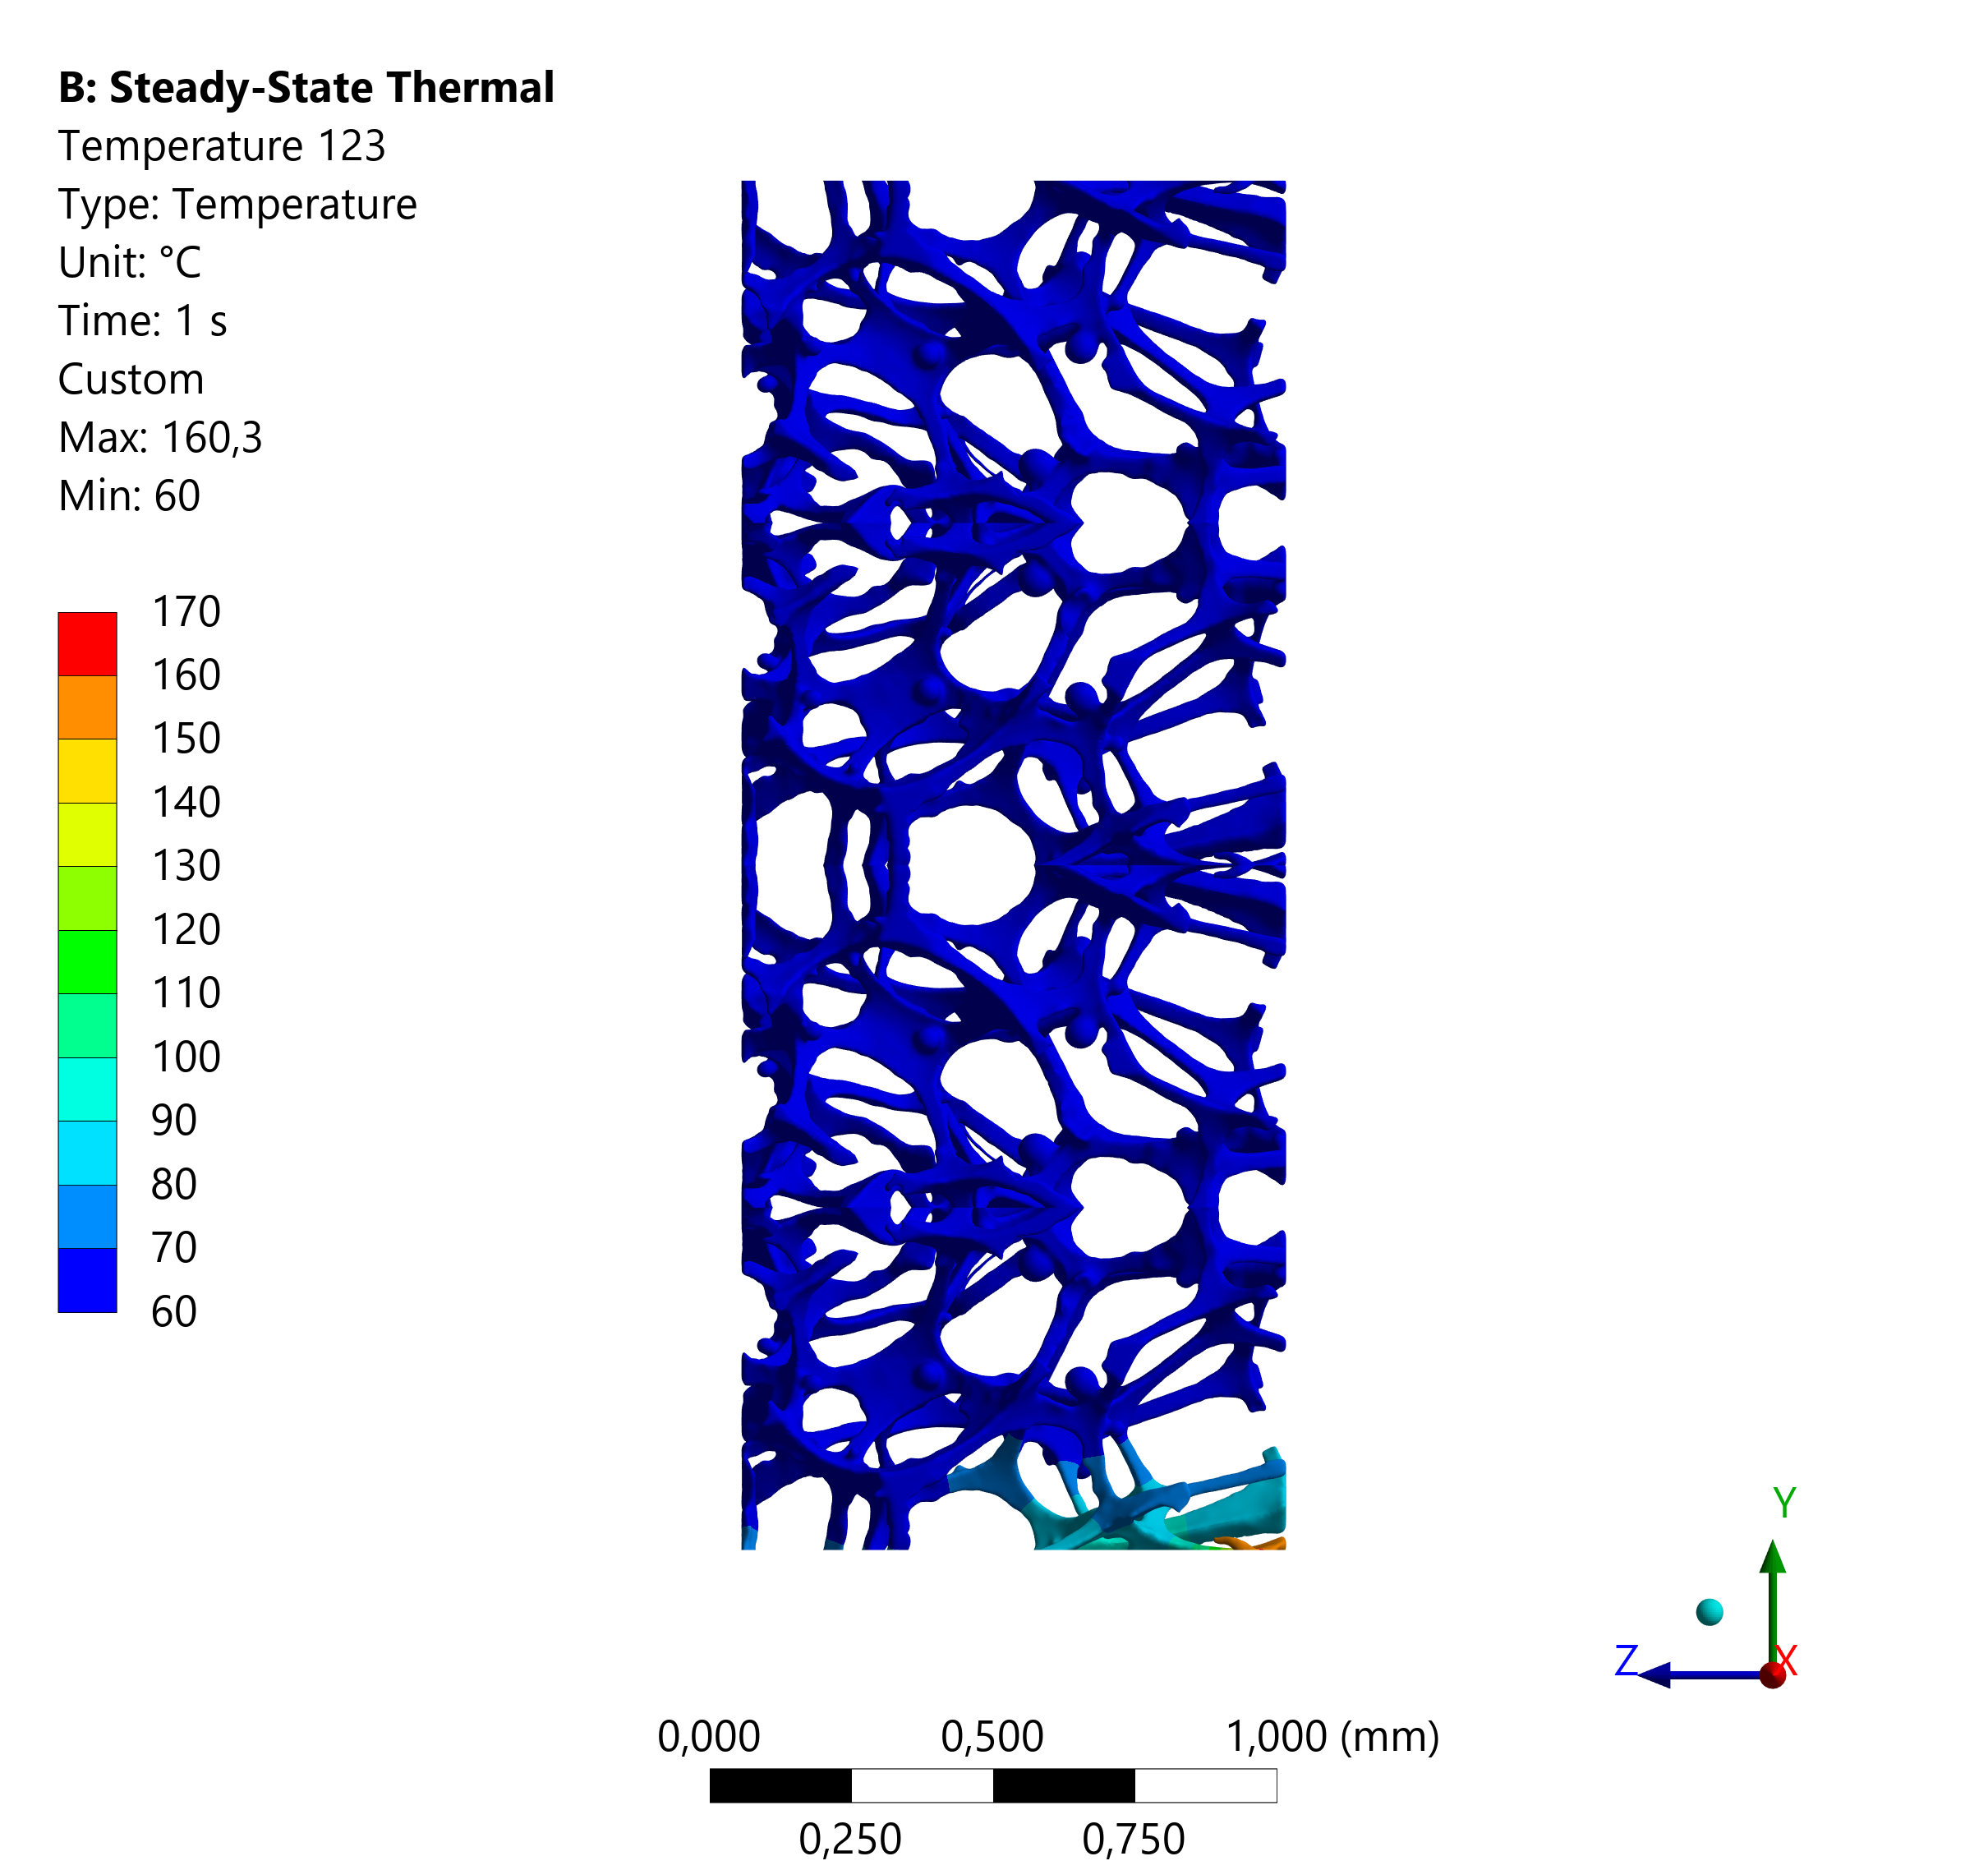
\includegraphics[width=\linewidth]{proudeni_mech34.png}
\caption{Temperature profile.}
\end{subfigure}
\hfill
\begin{subfigure}{0.35\textwidth}
\centering
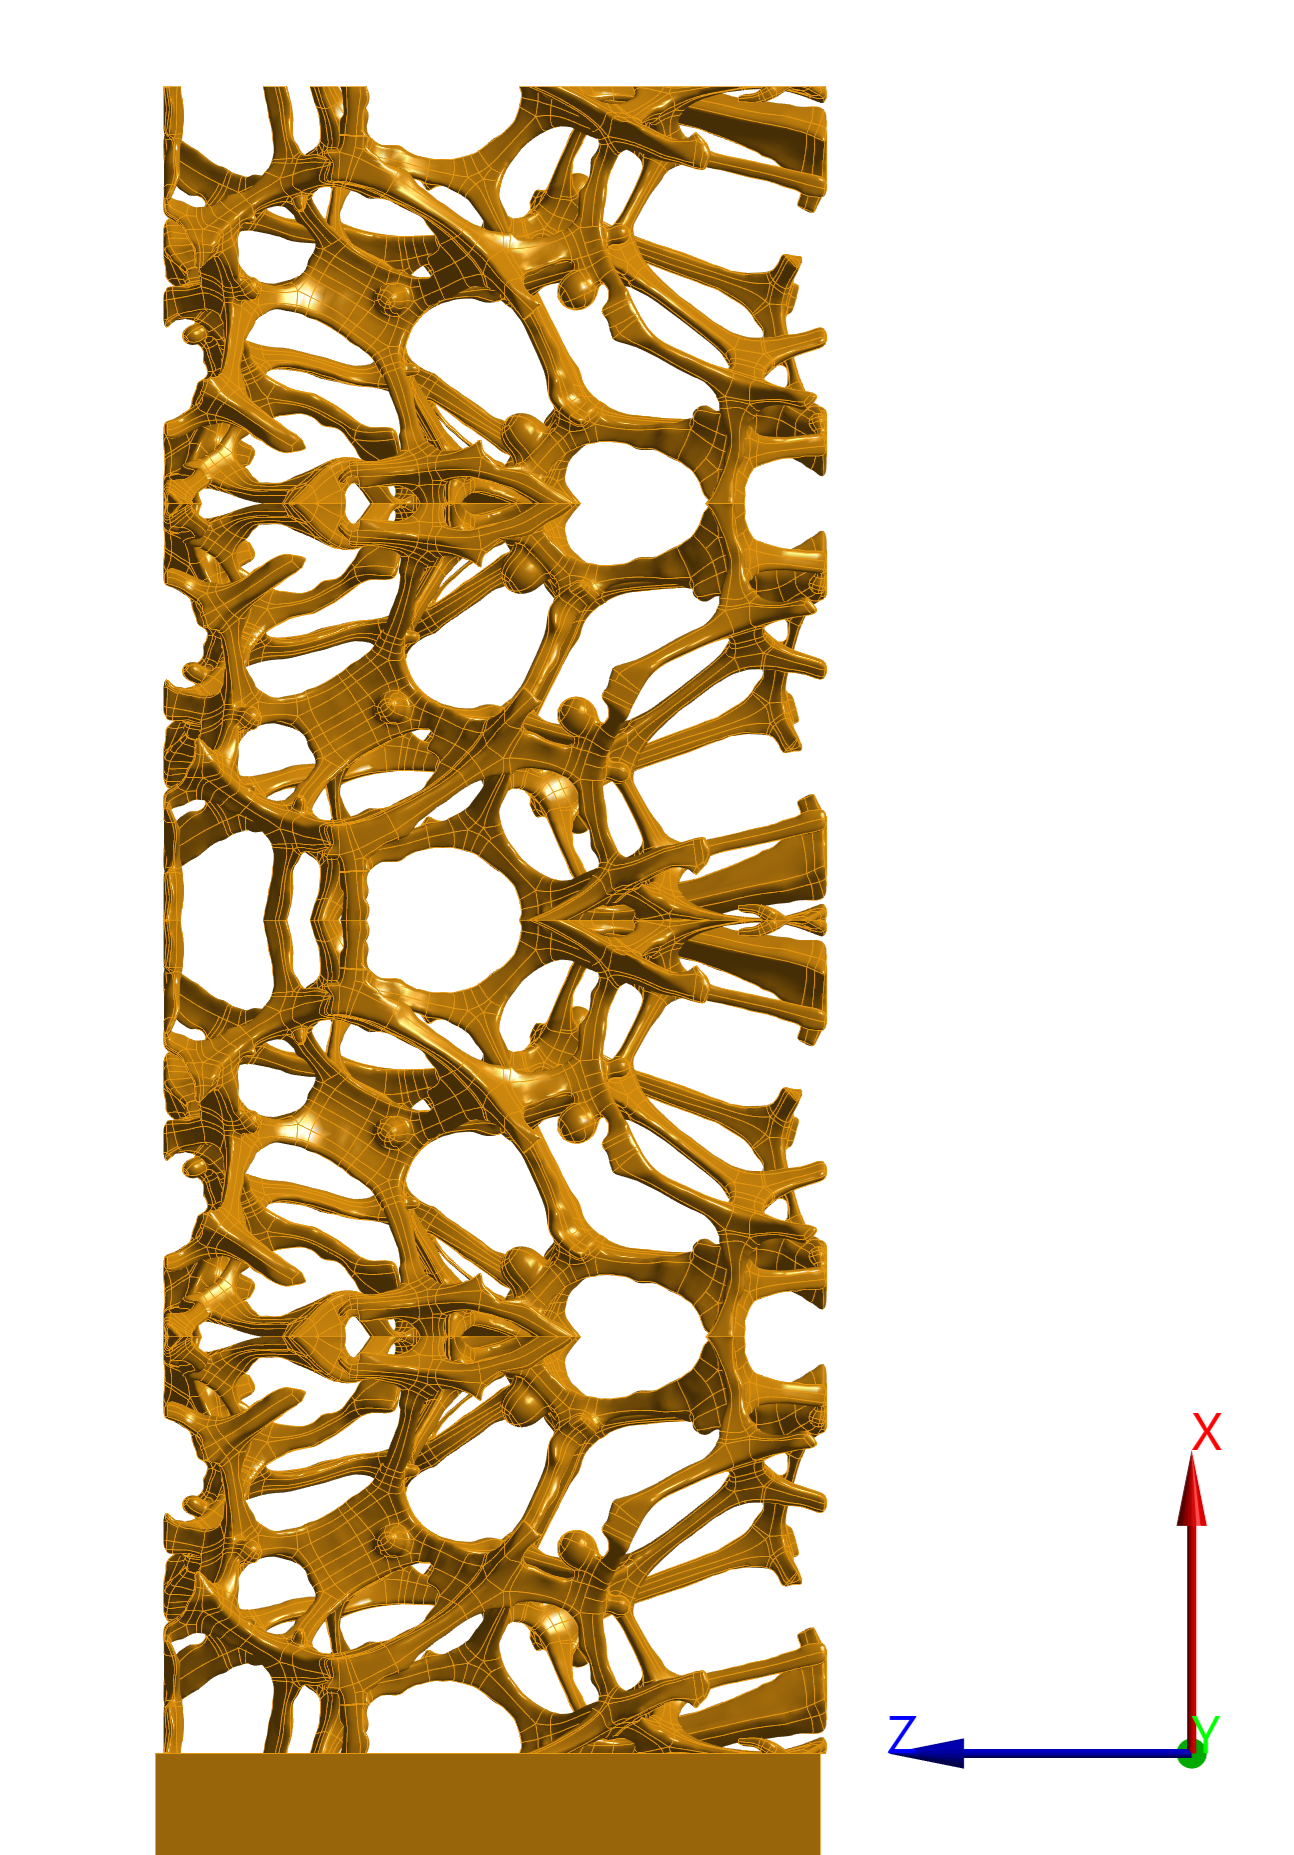
\includegraphics[width=\linewidth]{proudeni_mech35.png}
\caption{X coordinate definition.}
\end{subfigure}
\caption{Thermal analysis of the porous foam structure.}
\label{fig:profily_mech_xy}
\end{figure}

Figure \ref{fig:profily_mech_3x} shows an example of the temperature profile extracted from one of the cross sections within the porous foam structure.
The average temperature of each surface is calculated and plotted against the X coordinate.

\begin{figure}[H]
\centering
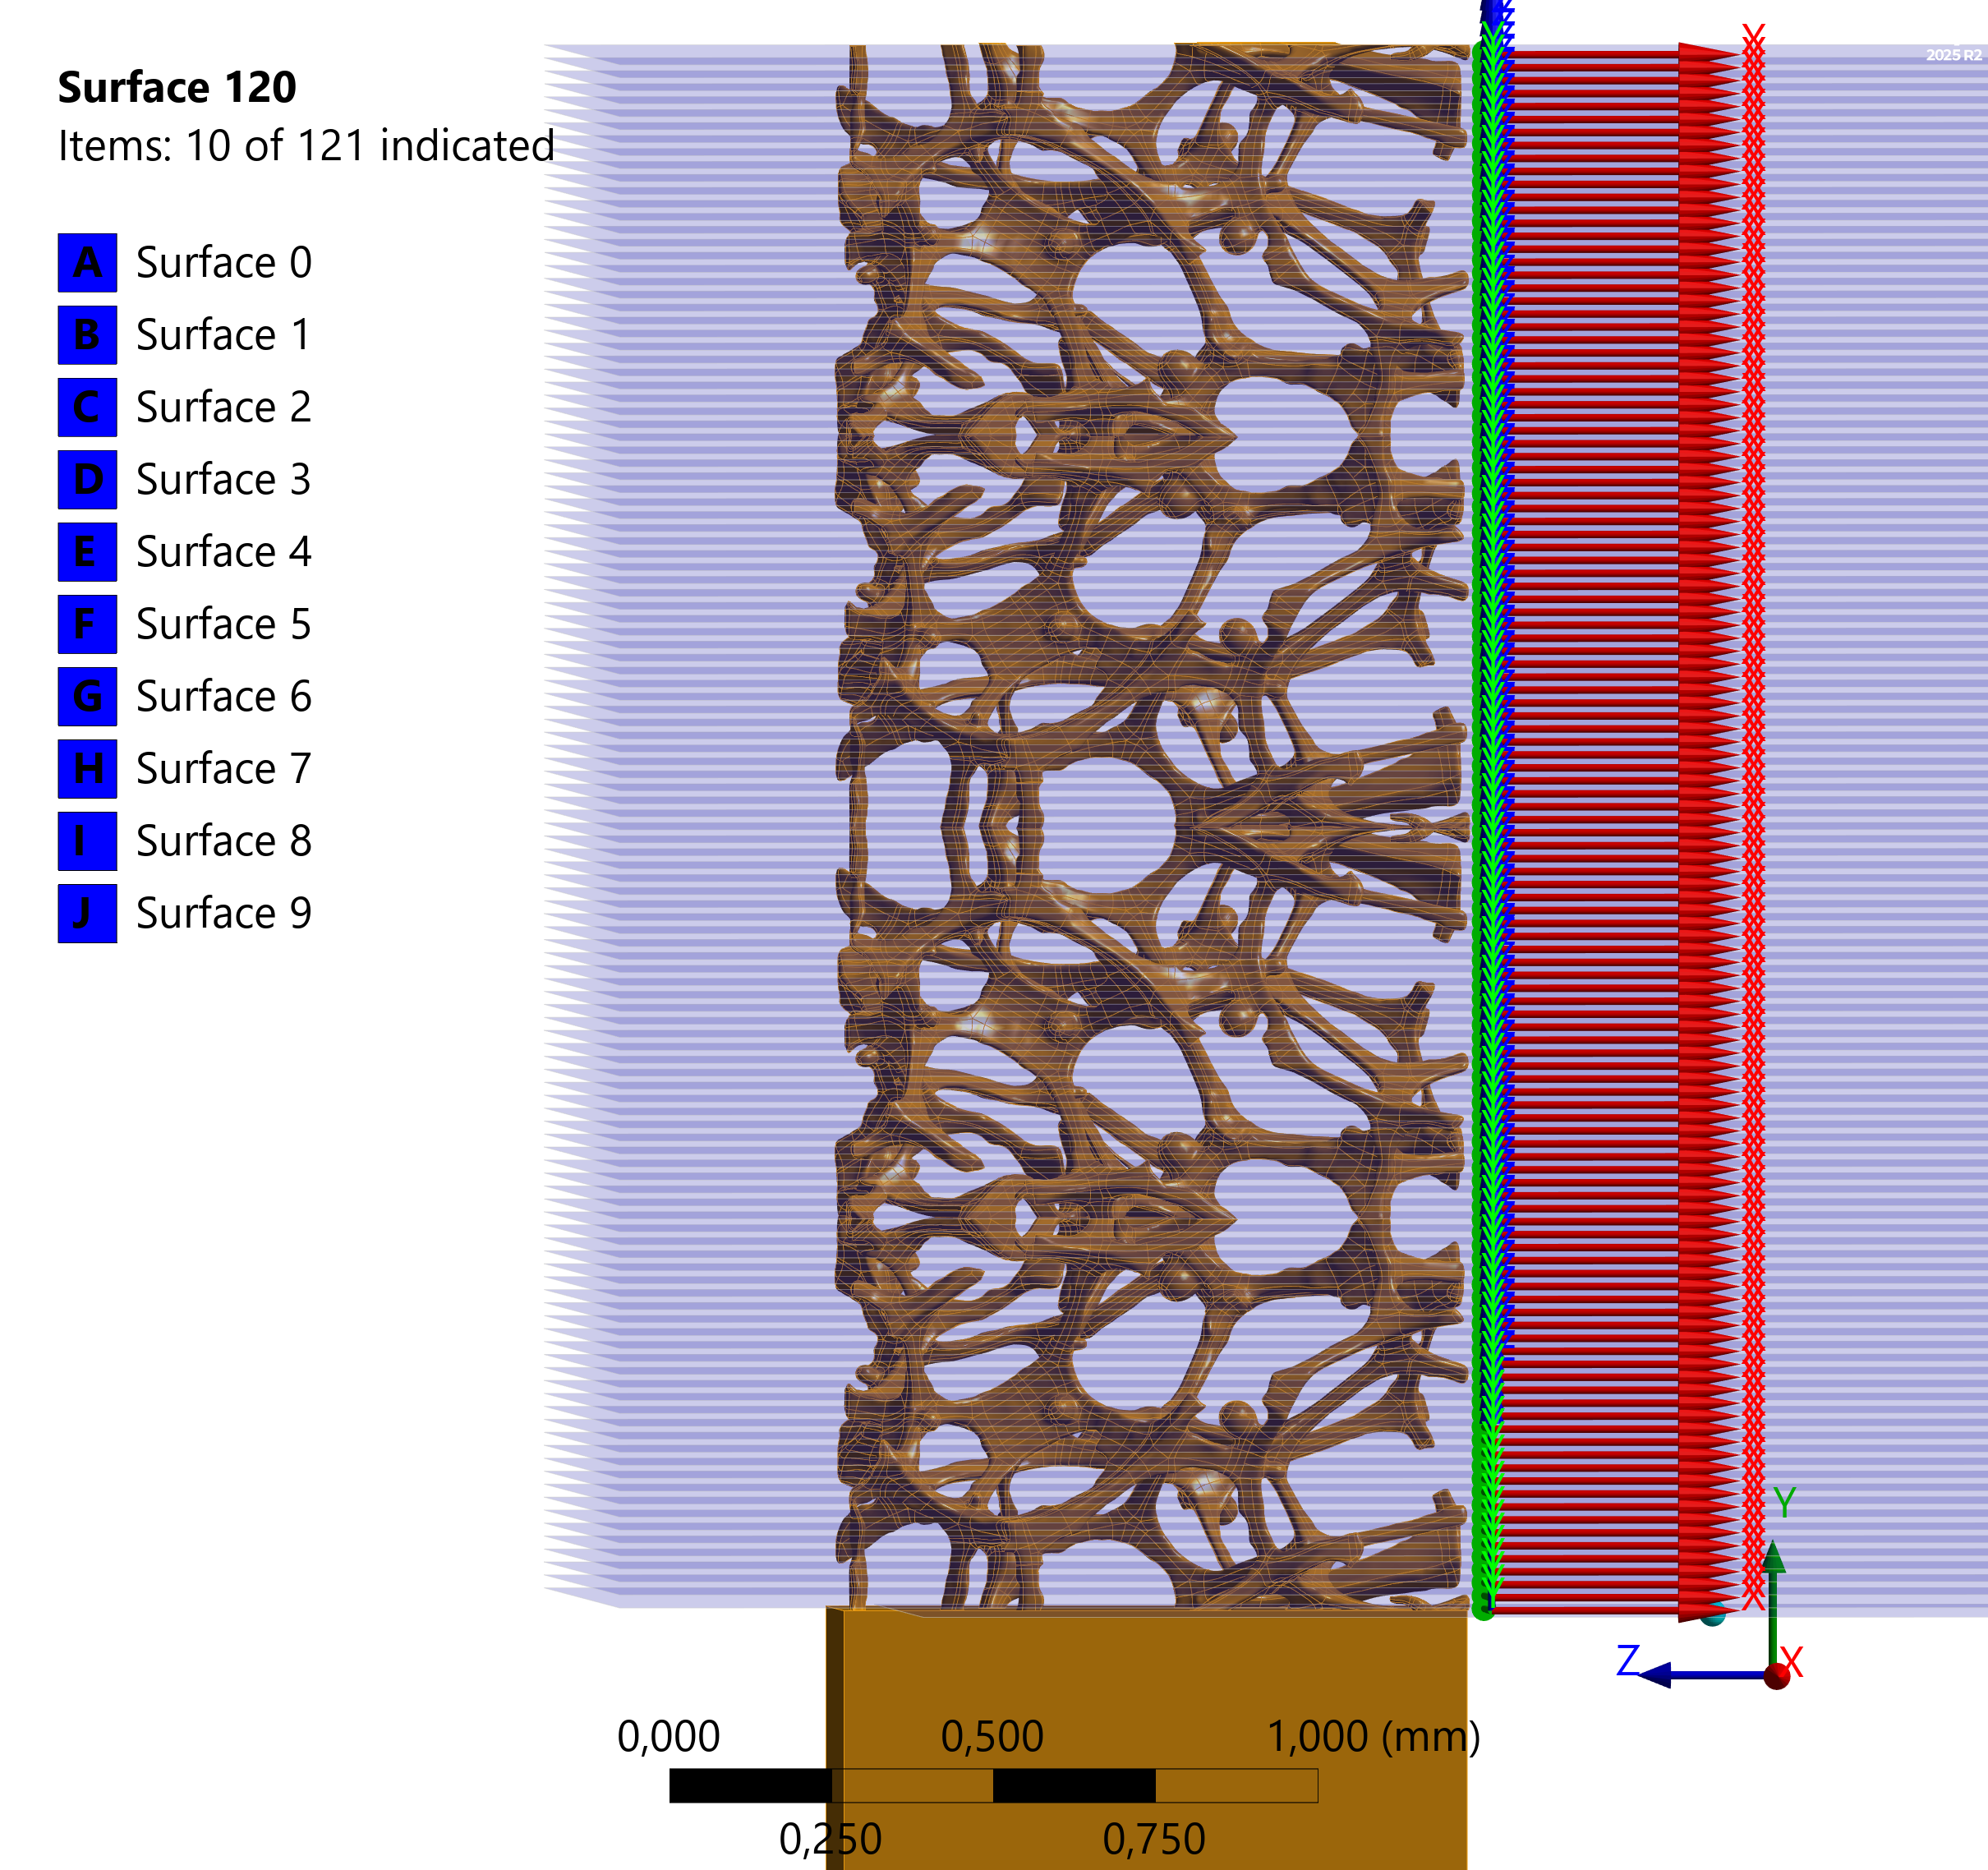
\includegraphics[width=0.85\linewidth, trim=0 0 0 21cm, clip]{mfl_2.png}
\caption{Set of 120 surfaces used for temperature profile extraction.}
\label{fig:profily_mech_4x}
\end{figure}

\begin{figure}[H]
\centering
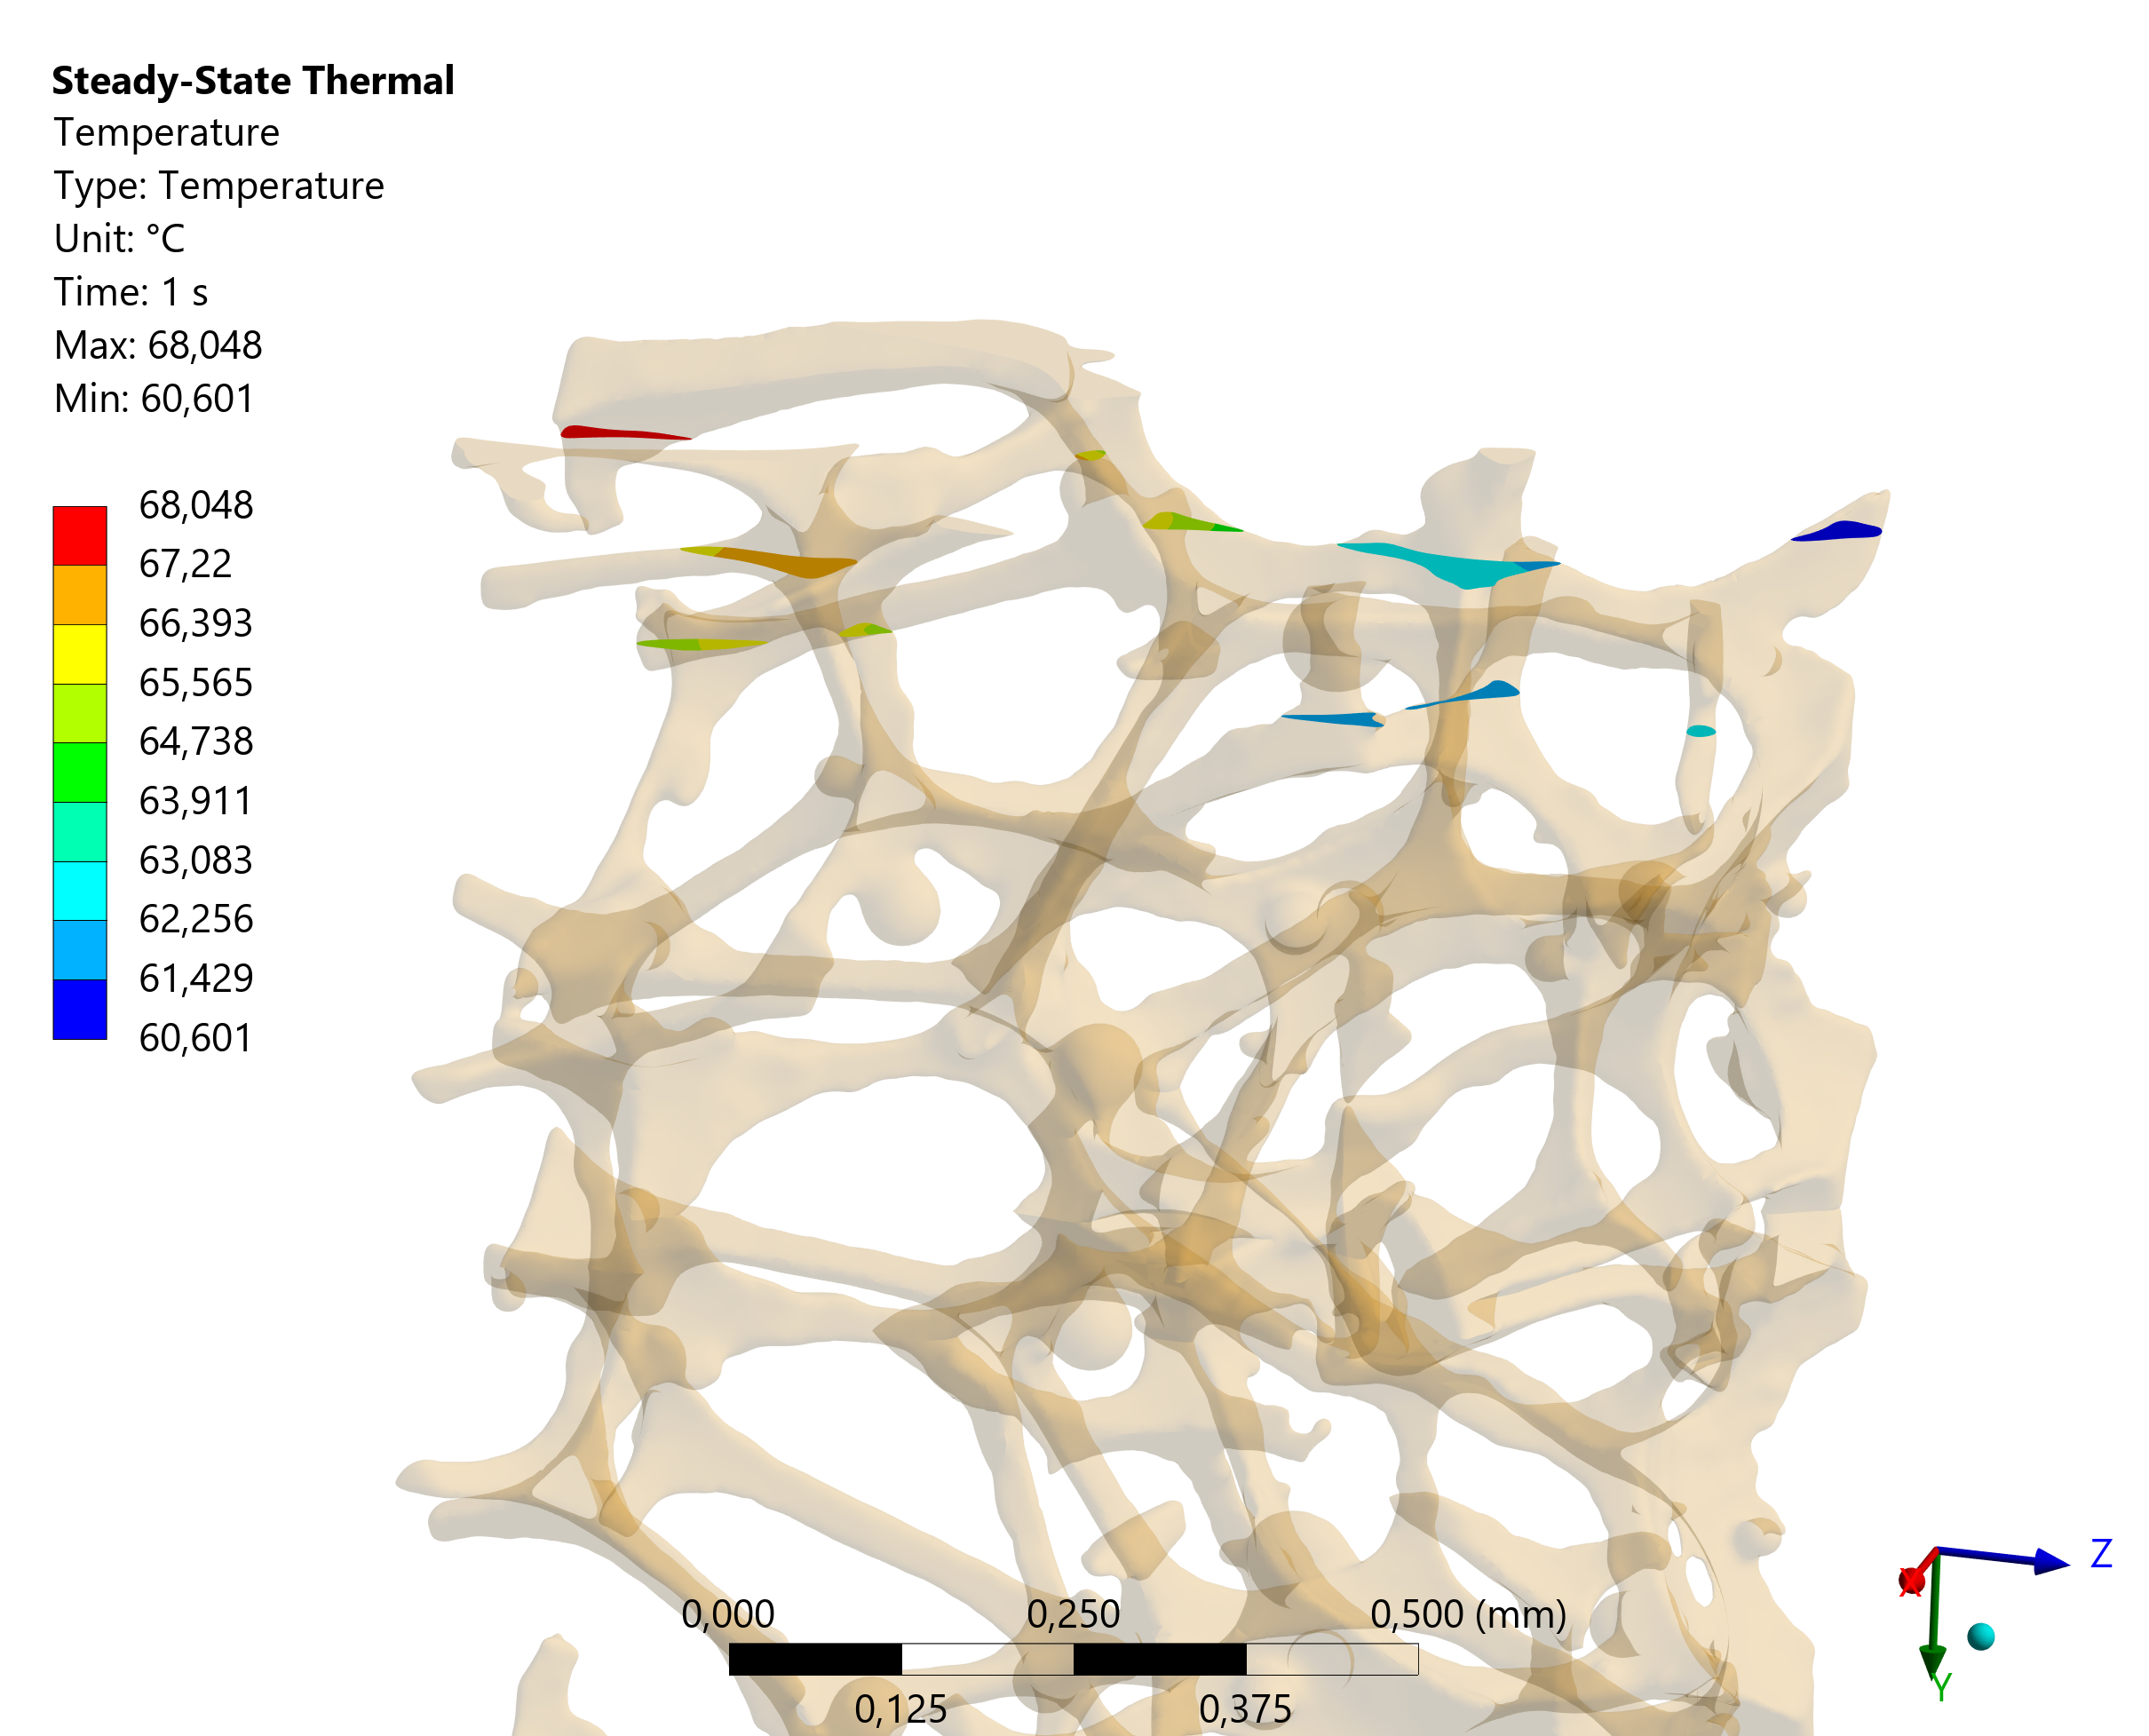
\includegraphics[width=0.9\linewidth, trim=0 12cm 0 0, clip]{proudeni_mech33.png}
\caption{Temperature profile in one of the cross sections.}
\label{fig:profily_mech_3x}
\end{figure}

Figures \ref{fig:profily_mech_1xx} and \ref{fig:profily_mech_2xx} show the temperature profiles within the porous foam structure under different operating conditions.
Figure \ref{fig:profily_mech_1xx} shows the temperature profiles at different inlet velocities for a constant heat flux load of 1~MW/m$^2$, Figure \ref{fig:profily_mech_2x} shows the temperature profiles at different heat flux loads for a constant inlet velocity of 0.1 m.s$^{-1}$.
The temperature reaches the surrounding fluid temperature in just under 1 mm from the heated surface for all considered scenarios.

\begin{figure}[H]
\centering
\begin{tikzpicture}
\begin{axis}[
    width=0.9\textwidth,
    height=0.34\textwidth,
    grid=both,
    xlabel={Temperature $\circ C$},
    ylabel={x Position $[mm]$},
    ymax=1.2,
    legend style={at={(0.98,0.98)},anchor=north east},
    every axis plot/.append style={line width=1.4pt},
]

\addplot table[x=A6, y=A0, col sep=semicolon] {nove_hodnoty.csv};
\addlegendentry{\phantom{0.}1\phantom{25} $\,\mathrm{m\,s^{-1}}$}

\addplot table[x=A5, y=A0, col sep=semicolon] {nove_hodnoty.csv};
\addlegendentry{\phantom{0}0.3 $\,\mathrm{m\,s^{-1}}$}

\addplot table[x=A4, y=A0, col sep=semicolon] {nove_hodnoty.csv};
\addlegendentry{\phantom{0}0.05 $\,\mathrm{m\,s^{-1}}$}

\end{axis}
\end{tikzpicture}
\caption{Foam temperature profiles at different inlet velocities, 1 $MW/m^2$}
\label{fig:profily_mech_1xx}
\end{figure}


\begin{figure}[ht]
\centering
\begin{tikzpicture}
\begin{axis}[
    width=0.9\textwidth,
    height=0.34\textwidth,
    grid=both,
    xlabel={Temperature $\circ C$},
    ylabel={x Position $[mm]$},
    ymax=1.2,
    legend style={at={(0.98,0.98)},anchor=north east},
    every axis plot/.append style={line width=1.4pt},
]

\addplot table[x=A3, y=A0, col sep=semicolon] {nove_hodnoty.csv};
\addlegendentry{\phantom{0.}2\phantom{25} $\,\mathrm{MW\,m^{-2}}$}

\addplot table[x=A2, y=A0, col sep=semicolon] {nove_hodnoty.csv};
\addlegendentry{\phantom{0.}1\phantom{25} $\,\mathrm{MW\,m^{-2}}$}

\addplot table[x=A1, y=A0, col sep=semicolon] {nove_hodnoty.csv};
\addlegendentry{\phantom{0}0.5 $\,\mathrm{MW\,m^{-2}}$}

\end{axis}
\end{tikzpicture}
\caption{Temperature profiles at different heat flux loads, $v_{inlet}=0.1 m.s^{-1}$}
\label{fig:profily_mech_2xx}
\end{figure}

\subsection{Results - heat exhaust}

The heat can be exhausted from the solid structure by two mechanisms: convection through the solid wall and through the porous foam structure.
Figure \ref{fig:heat_mech_conv2} shows the two convection boundary conditions applied on the foam and the wall surfaces in the thermal model.
It is important to evaluate the ratio of heat exhausted by each mechanism, as it provides insight into the effectiveness of the porous foam structure in enhancing heat transfer.

\begin{figure}[H]
\centering
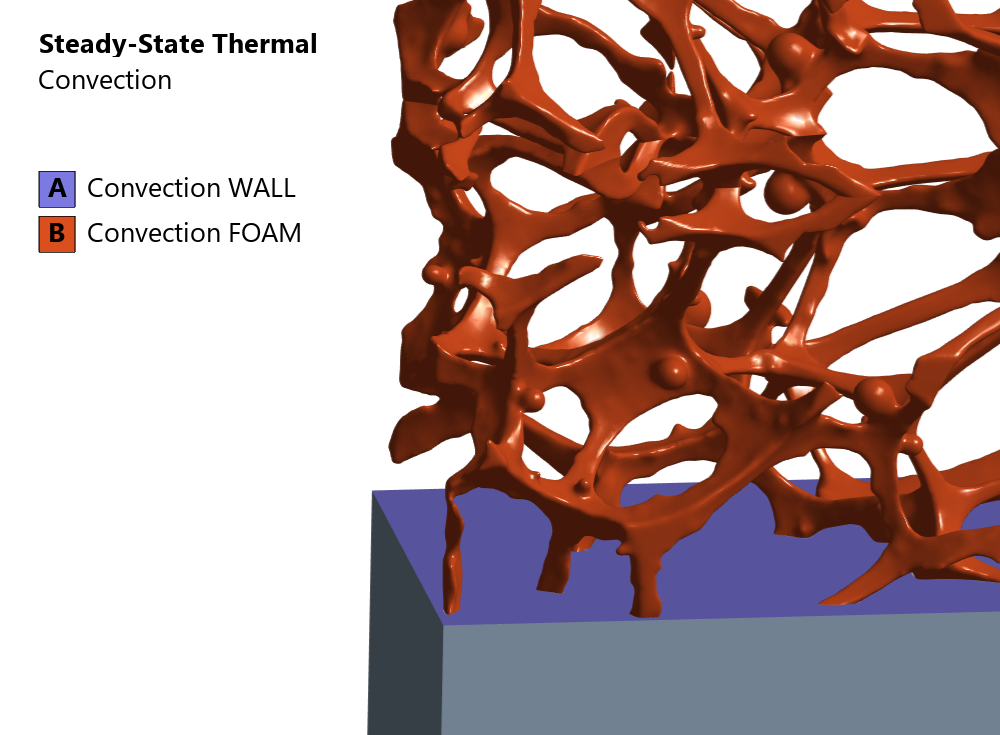
\includegraphics[width=0.56\linewidth]{mfl_3.png}
\caption{2 convection boundary conditions applied on the foam and the wall surfaces.}
\label{fig:heat_mech_conv2}
\end{figure}

The ratio of heat exhausted by each mechanism is influenced by the inlet flow velocity.
Figure \ref{fig:pomer_exhaust} shows the ratio of total heat exhausted by the porous foam structure as a function of inlet velocity.
The convection on porous foam surface is more dominant in the lower velocity range, while the convection on the solid channel wall surface becomes major at higher velocities.
This effect corresponds to the relation between the heat transfer coefficients on both surfaces, as shown in Figure \ref{fig:flumech_alpha_dist_v}, and the thermal conductivity of copper.
At lower velocities, the conductivity in the solid volume is relatively high compared to the convection on the surface, allowing the heat to reach higher in the porous foam structure - increasing the effect of convection on the foam surface.
Higher velocities increase the heat transfer coefficient and the heat is exhausted sooner before it can reach higher in the foam structure.

\begin{figure}[H]
\centering
\begin{tikzpicture}
\begin{axis}[
    width=0.9\textwidth,
    height=0.45\textwidth,
    grid=both,
    xlabel={Flow velocity $[m/s]$},
    ylabel={Ratio of exhausted heat $[\%]$},
    xmin=0, xmax=1,
    ymin=0, ymax=100,
    legend style={at={(0.98,0.98)},anchor=north east},
    every axis plot/.append style={line width=1.4pt},
]

% -------------------------------------------------
% hranice regionů (NE celé osy!)
% -------------------------------------------------
\addplot[name path=topA, draw=none]
coordinates {(0,100) (1,100)};

\addplot[name path=bottomB, draw=none]
coordinates {(0,0) (1,0)};

% -------------------------------------------------
% hlavní křivka
% -------------------------------------------------
\addplot[
    name path=curve,
    color=black,
]
table[x=x, y=y, col sep=semicolon] {pomer_heat_foam.csv};


% -------------------------------------------------
% Region A – NAD křivkou
% -------------------------------------------------
\addplot[
    draw=none,
    fill=blue!20,
    opacity=0.35,
]
fill between[of=curve and topA];

% -------------------------------------------------
% Region B – POD křivkou
% -------------------------------------------------
\addplot[
    draw=none,
    fill=red!25,
    opacity=0.45,
]
fill between[of=bottomB and curve];

% -------------------------------------------------
% popisky regionů (s pozadím)
% -------------------------------------------------
\node[
    fill=white,
    fill opacity=0.85,
    text opacity=1,
    inner sep=2pt,
    font=\bfseries
] at (axis cs:0.45,55) {Convection on channel wall surface.};

\node[
    fill=white,
    fill opacity=0.85,
    text opacity=1,
    inner sep=2pt,
    font=\bfseries
] at (axis cs:0.29,9) {Convection on porous foam surface.};

\end{axis}
\end{tikzpicture}
\caption{Ratio of total heat exhausted by the porous foam structure.}
\label{fig:pomer_exhaust}
\end{figure}


\pagebreak



\subsection{Effective height of the porous foam heat sink}

To evaluate the performance of the porous foam heat sink, the concept of effective height is introduced.
The effective height $\boldsymbol{h_{\text{eff90}}}$ is defined as the height in the foam structure where 90~\% of the total heat transfer occurs.
Figure \ref{fig:profily_mech_1x} shows an example of determining the effective height from the temperature profile at an inlet velocity of 0.05~m/s and load of 1~MW/m$^2$.
The effective height is determined by finding the position along the x-axis where the temperature reaches 90~\% of the maximum temperature difference in the foam structure.
This effective height provides a useful metric for comparing the performance of different boundary conditions.

\begin{figure}[H]
\centering
\begin{tikzpicture}
\begin{axis}[
    width=0.9\textwidth,
    height=0.4\textwidth,
    grid=both,
    xlabel={Temperature $^\circ C$},
    ylabel={x Position $[mm]$},
    ymax=0.8,
    ymin=0,
    xmin=55,
    legend style={at={(0.98,0.98)},anchor=north east},
    every axis plot/.append style={line width=1.4pt},
]

% hlavní křivka
\addplot table[x=A4, y=A0, col sep=semicolon,color=red] {nove_hodnoty.csv};
\addlegendentry{\phantom{0}0.05 $\,\mathrm{m\,s^{-1}}$}

% vertikální čára x = 64.5
\addplot [
    black,
    dashed,
    line width=1pt
] coordinates {(64.5,0) (64.5,0.38)};


% vertikální čára x = 64.5
\addplot [
    black,
    line width=1pt
] coordinates {(55,0.38) (64.5,0.38)};

\addplot[
    only marks,
    mark=o,
    mark size=4pt,
    very thick,
    color=black
]
coordinates {(64.5,0.38)}
node[
    anchor=south west
] {$\boldsymbol{h_{\text{eff90}}=0.38\,\mathrm{mm}}$};


\end{axis}
\end{tikzpicture}
\caption{Effective height definition example for inlet velocity 0.05~m/s.}
\label{fig:profily_mech_1x}
\end{figure}

Figure \ref{fig:profily_mech_2x} shows the effective height of the foam heat sink as a function of inlet velocity for different heat flux loads.
The effective height decreases with increasing inlet velocity, indicating that only a very thin layer of the foam structure is actively involved in heat transfer at higher flow rates.
This trend highlights the importance of optimizing the foam structure and flow conditions to maximize the effective height and overall heat transfer performance of the porous foam heat sink.
It can be concluded that the porous foam volume higher than the effective height is not contributing to the heat transfer process, therefore the design of the cooling channel can be optimized by reducing the foam height to the effective height.

\begin{figure}[ht]
\centering
\begin{tikzpicture}
\begin{axis}[
    width=0.9\textwidth,
    height=0.5\textwidth,
    grid=both,
    xlabel={Flow velocity $[m/s]$},
    ylabel={Effective height $\boldsymbol{h_{\text{eff90}}}$ $[mm]$},
    legend style={at={(0.98,0.98)},anchor=north east},
    every axis plot/.append style={line width=1.4pt},
]

\addplot table[x=x, y=05heff90, col sep=semicolon, color=red] {heff_vysledky.csv};
\addlegendentry{\phantom{0.}2\phantom{25} $\,\mathrm{MW\,m^{-2}}$}
\addplot table[x=x, y=1heff90, col sep=semicolon, color=black] {heff_vysledky.csv};
\addlegendentry{\phantom{0.}1\phantom{25} $\,\mathrm{MW\,m^{-2}}$}
\addplot table[x=x, y=2heff90, col sep=semicolon, color=blue] {heff_vysledky.csv};
\addlegendentry{\phantom{0.}0.5\phantom{25} $\,\mathrm{MW\,m^{-2}}$}

\end{axis}
\end{tikzpicture}
\caption{Effective height of the foam heat sink as a function of inlet velocity.}
\label{fig:profily_mech_2x}
\end{figure}


\pagebreak

\section{Porous material cooling channel - critical heat flux study}


The application of porous materials as an enhancement technique for high heat flux cooling has attracted considerable attention in recent years due to several mechanisms that may improve the thermal performance of cooling channels. The most straightforward explanation is the substantial increase in the effective heat transfer surface provided by the porous structure. Compared to a smooth cooling channel, the large internal surface area promotes convective heat transfer between the solid matrix and the coolant, allowing more efficient removal of thermal energy from the heated wall.
\\
\\
However, from the perspective of fusion reactor cooling, the potentially more significant advantage of porous materials is their influence on boiling heat transfer and the critical heat flux (CHF). Conventional cooling channels are ultimately limited by the formation of a continuous vapour layer on the heated surface. Once this vapour blanket is established, the thermal contact between the wall and the liquid coolant rapidly deteriorates, resulting in a sharp increase in wall temperature and a dramatic reduction in heat removal capability.
\\
\\
Several physical mechanisms have been proposed to explain the observed CHF enhancement in porous structures. One of the most frequently discussed effects is the capillary pumping generated by the interconnected porous network. Surface tension forces continuously transport liquid coolant through the pores towards locally dried regions of the heated surface, improving rewetting and delaying the formation of stable dry spots. As a consequence, the heated surface remains wetted over a wider operating range than in conventional smooth channels.
\\
\\
Another proposed mechanism is the modification of the local flow structure inside the porous medium. The complex three-dimensional geometry promotes intensive mixing of the liquid and vapour phases, suppresses the formation of large continuous vapour channels and encourages the detachment of small vapour bubbles. This enhanced phase interaction prevents the development of an insulating vapour blanket and contributes to maintaining efficient liquid contact with the heated surface.
\\
\\
Although these mechanisms have been reported in the literature, their relative contribution strongly depends on the porous morphology, pore size, permeability, operating pressure and coolant velocity. Consequently, the heat transfer behaviour of porous cooling channels cannot be reliably predicted solely from existing correlations, and experimental validation remains essential.
\\
\\
The following section therefore presents the proof-of-concept experimental investigation performed within this work. The objective of the experiments is to evaluate whether a porous material integrated into the cooling channel can effectively delay the onset of critical heat flux under representative operating conditions and to assess its potential applicability for future plasma-facing components in nuclear fusion reactors.

\pagebreak
\subsection{Proof of concept experimental study}
The proof-of-concept measurements were performed on the Heat Flux Experimental Loop (HEFEL), a recirculating water loop developed for high-heat-flux testing of actively cooled samples \mycite{Smolk2023}. The loop provides controlled coolant flow through a replaceable test section while the specimen is heated by electromagnetic induction. Coolant conditions and solid temperatures are monitored during the test, enabling both hydraulic characterization and identification of the onset of boiling crisis.

For the present campaign, water was supplied to the test section at 70~kPa and an inlet temperature of 60~$^\circ$C. Hydraulic measurements were first carried out over a variable flow range to determine the pressure-drop characteristic of each sample. The subsequent high-heat-flux comparison used a fixed volumetric flow rate of 6~L/min, corresponding to an average velocity of approximately 0.25~m/s in the channel sample area. These boundary conditions are summarized in Table~\ref{tab:hefel_parameters}.

\begin{table}[ht!]
\centering
\begin{tabular}{|l|c|}
\hline
Working fluid & Water \\
\hline
Test-section pressure & 70~kPa \\
\hline
Inlet coolant temperature & 60~$^\circ$C \\
\hline
High-heat-flux test flow rate & 6~L/min \\
\hline
Average channel velocity & approximately 0.25~m/s \\
\hline
Heating method & Electromagnetic induction \\
\hline
\end{tabular}
\caption{HEFEL operating parameters used in the proof-of-concept CHF study.}
\label{tab:hefel_parameters}
\end{table}

\begin{figure}[ht!]
  \centering
  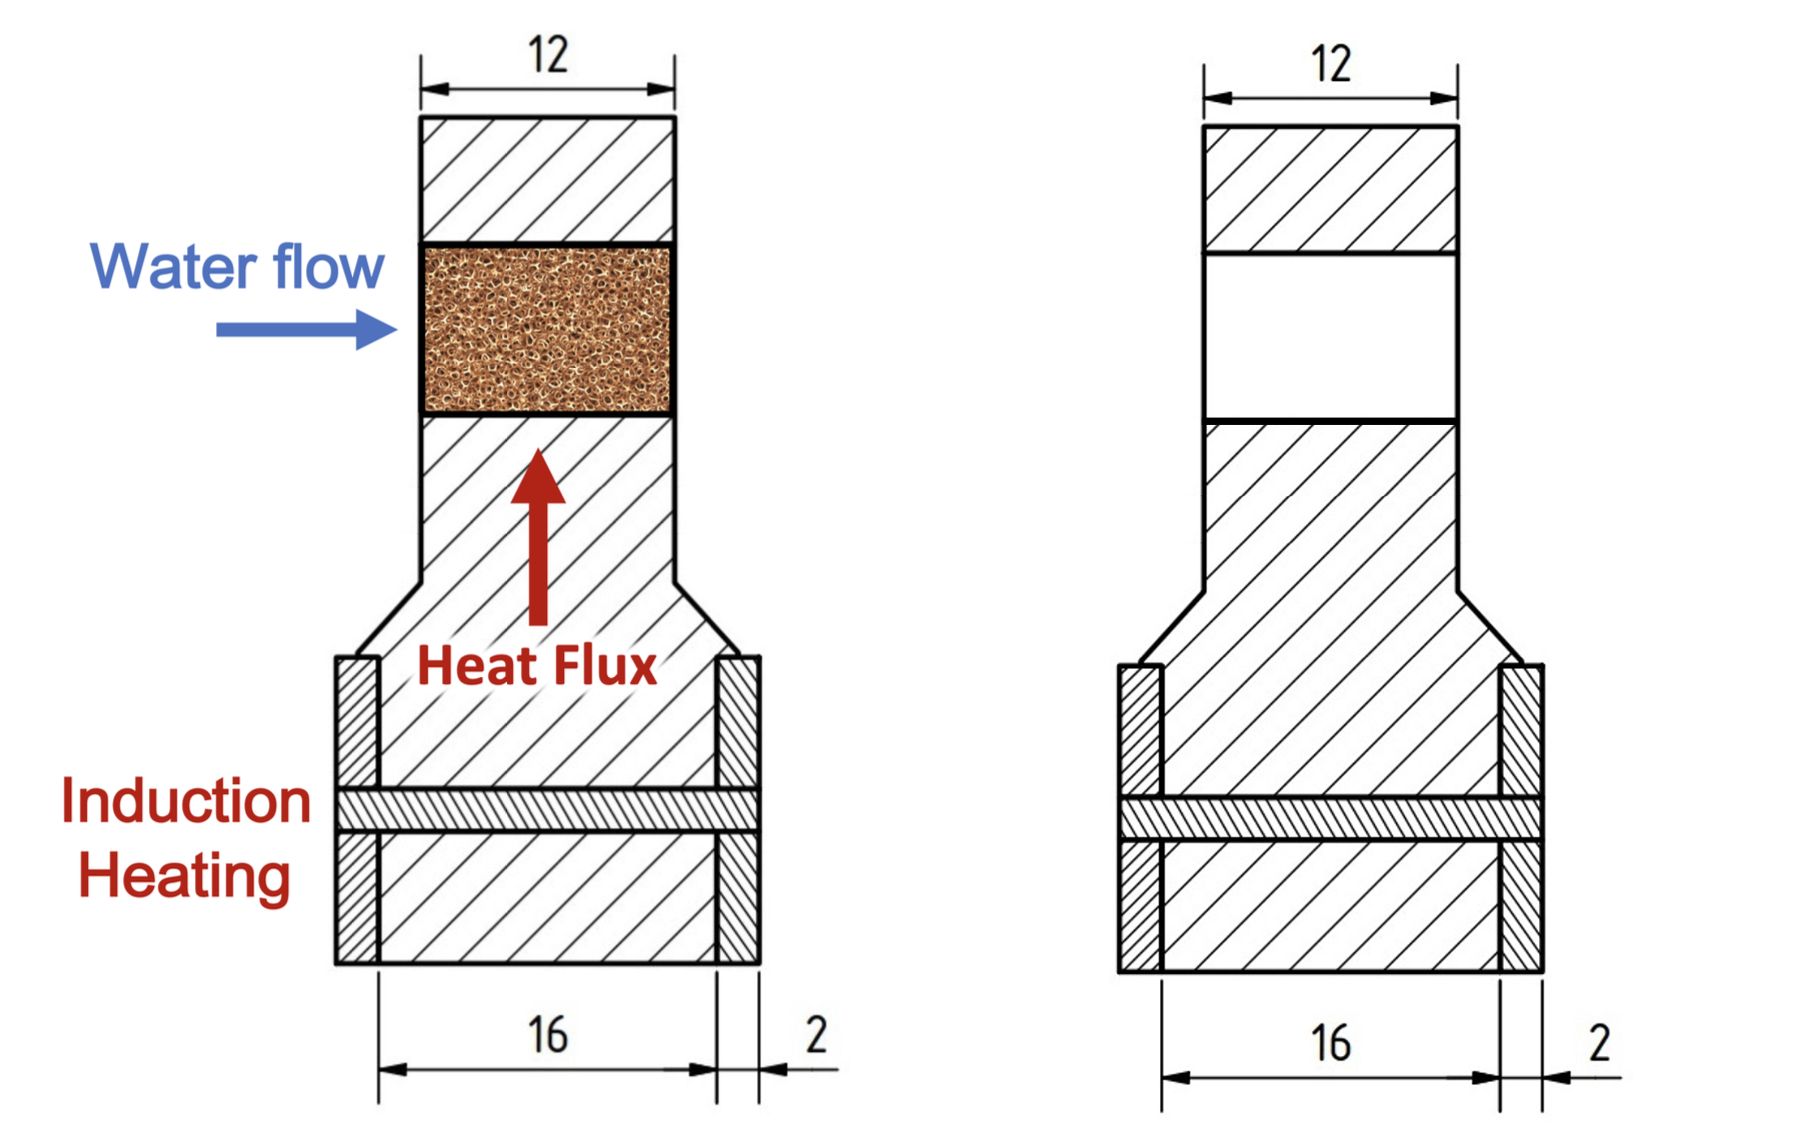
\includegraphics[width=12cm]{chf_1.png} 
  \caption{Porous channel sample (left) and plain channel sample (right) \cite{Smolk2024}.}
  \label{fig:chf_sample}
\end{figure}

Figure \ref{fig:chf_sample} shows the schematic comparison of two manufactured samples.
The cooling channel sample is made of CuCrZr, steel plates are attached to increase the efficiency of induction heating, and porous copper is soldered directly to the CuCrZr body.
Thermocouples are inserted into the CuCrZr sample body to measure the solid temperature in various positions.
 Figure \ref{fig:chf_vykres} shows the manufactured test specimens and their instrumentation. The samples were installed in the HEFEL test section under identical hydraulic boundary conditions.

\begin{figure}[ht!]
  \centering
  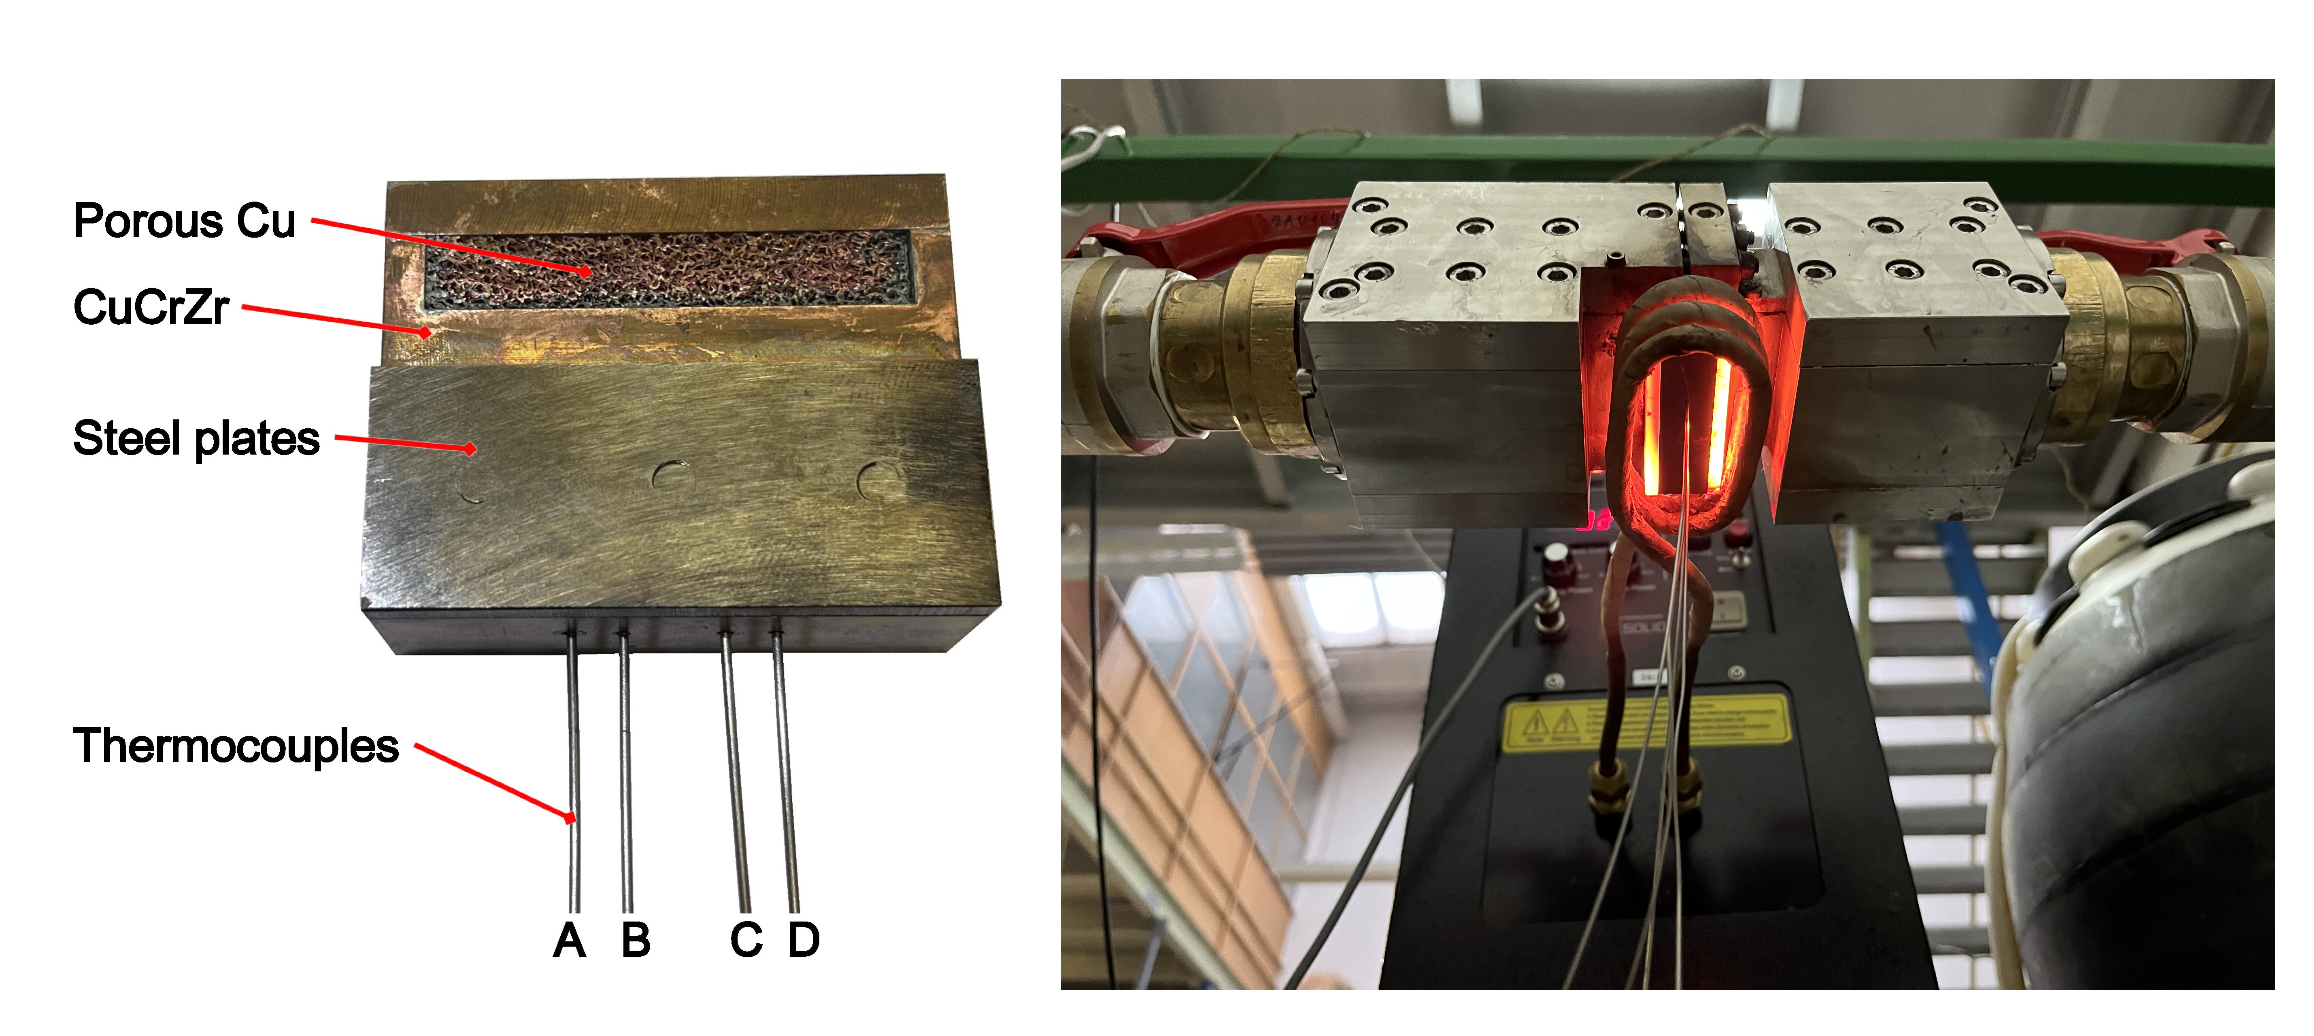
\includegraphics[width=12cm]{chf_2.png} 
  \caption{Porous channel sample (left) and plain channel sample (right).}
  \label{fig:chf_vykres}
\end{figure}

\subsubsection{Material analysis}
A porosity of 95.2~\%, measured by helium pycnometry, was corroborated by density measurements (0.443 g/cm$^3$), the standard deviation of porosity measurement is 0.2~\%.
Wavelength-dispersive spectroscopy (WDS) confirmed that the porous material is pure copper, no additional elements were found (Figure \ref{fig:pory}(right)).
The results of the pore diameter analysis are shown in Figure \ref{fig:pory} (left), the mean pore diameter is 0.56 mm.
The diameter of the strut is 60 $\mu$ m. The properties measured of the porous material and the calculated values of permeability and Forchheimer coefficient are listed in Table 1.

\begin{figure}[ht!]
    \centering
    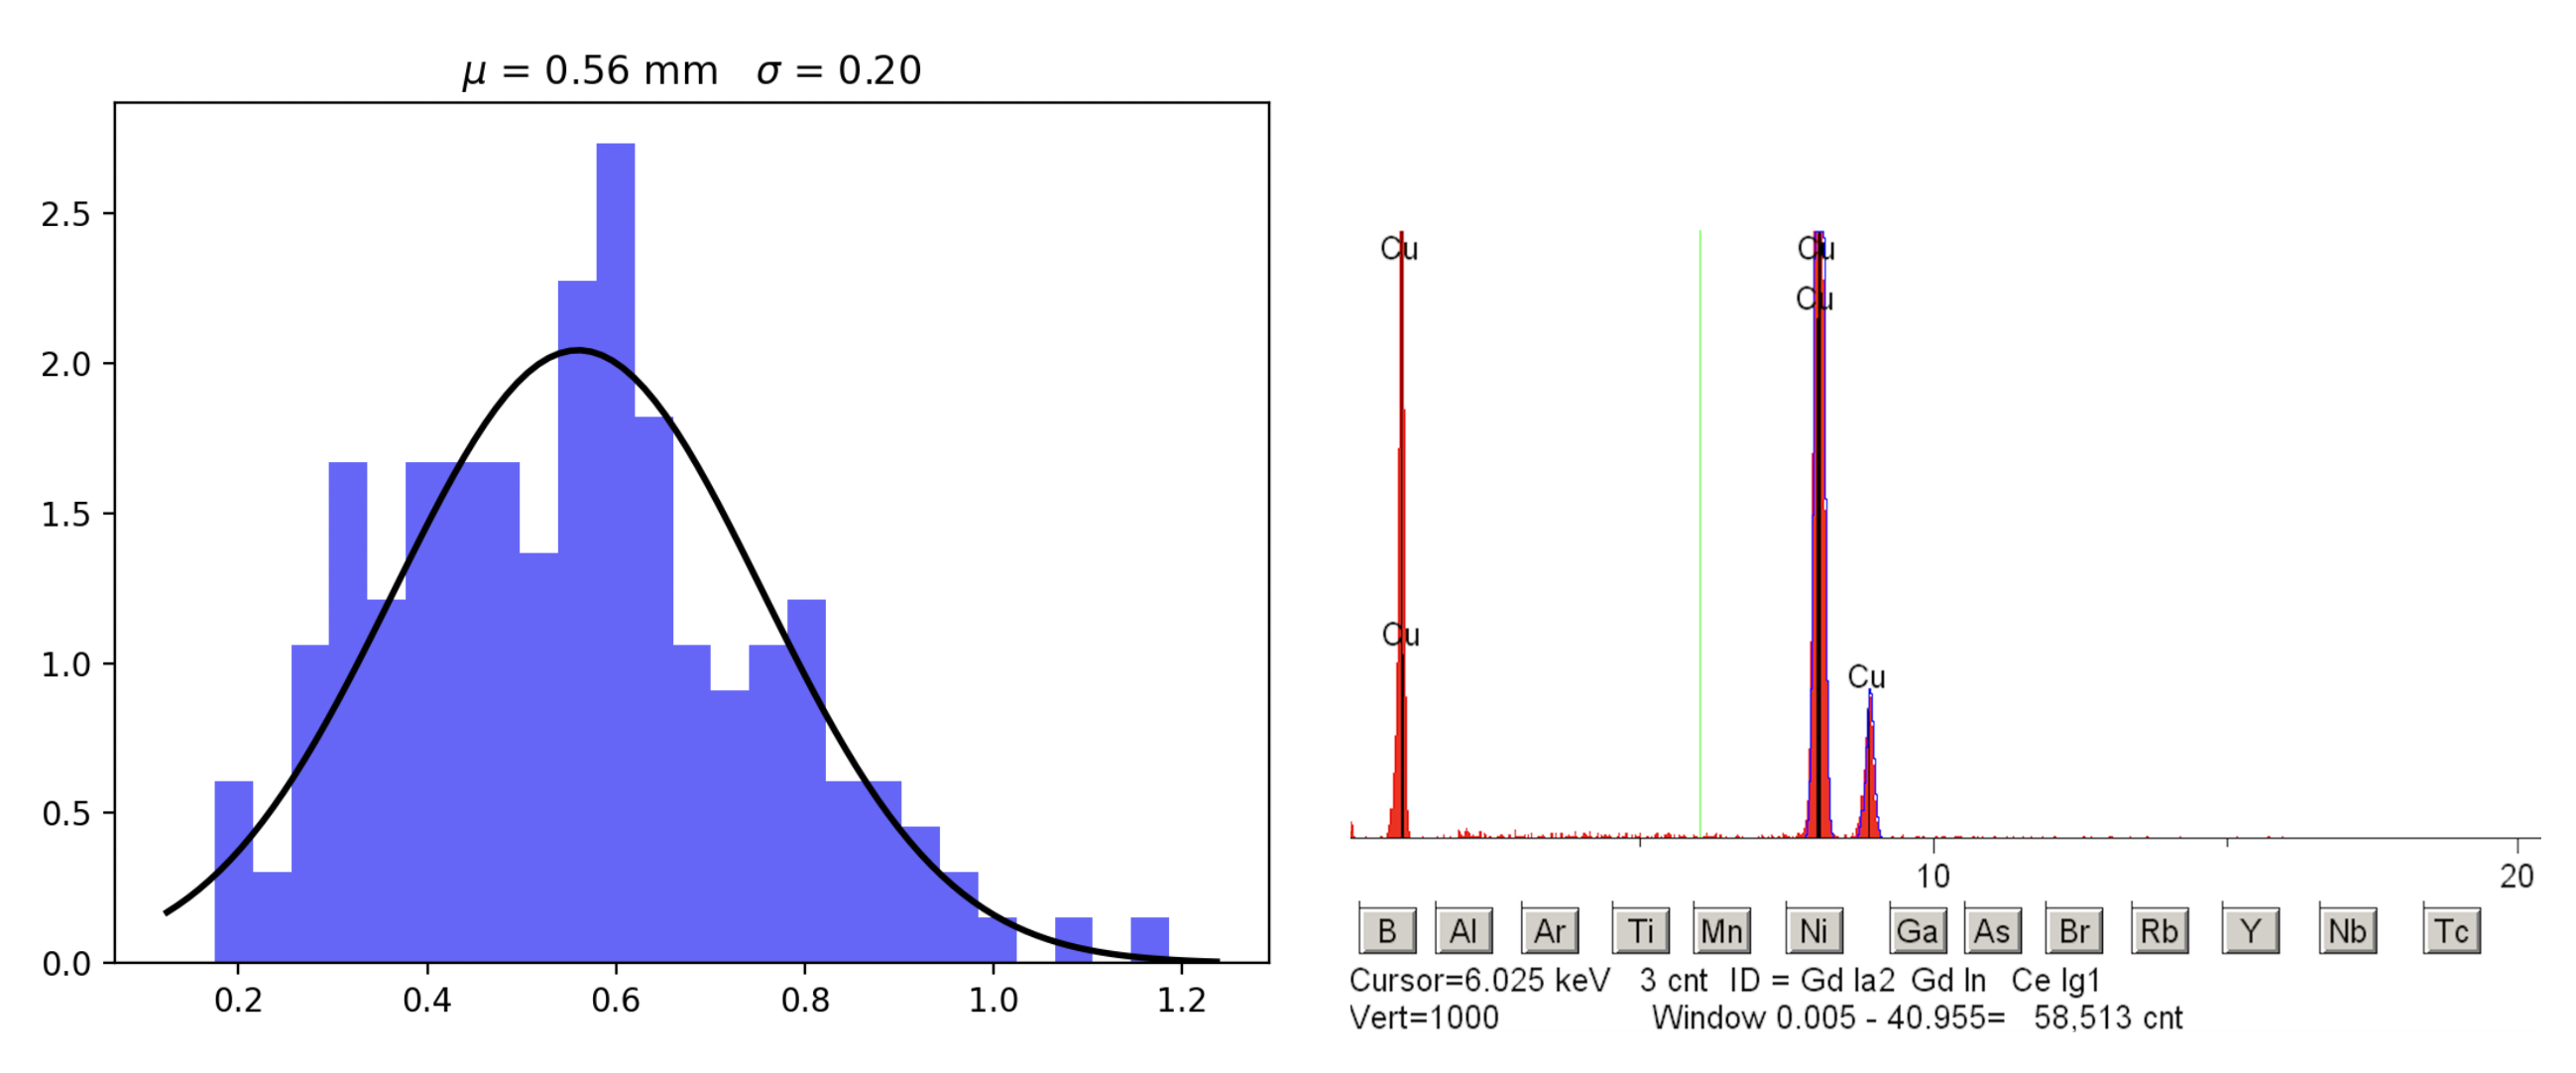
\includegraphics[width=14cm]{chf_4.png}
    \caption{Mean pore diameter $d_p$ analysis results (left) and WDS analysis (right).}
    \label{fig:pory}
\end{figure}

\begin{center}
  \begin{table}[ht!]
    \centering
  \begin{tabular}{|c|c|c|c|c|}
      \hline
      Pore diameter& Strut diameter & Porosity & Forchheimer c. & Permeability\\
      \hline
      $d_p$ [mm] & $d_f$ [mm] & $\epsilon  [\%]$ & c [m$^{2}$] & K [-]\\
      \hline
      0.56& 0.6 & 95.2 & 0.1206624 & 4.725199 . 10$^{-9}$ \\
      \hline
  \end{tabular}
  \caption{Measured porous material properties.}
  \end{table}
\end{center}


Figure \ref{fig:provoz} shows the porous copper structure after experimental measurements (after 3 hours of operation).
No significant damage to the structure itself is observed, but the formation of corrosives and impurities is clearly visible.
 Figure \ref{fig:provoz} (right) shows the detailed image of the soldered joint.
Although the porous structure is observed to be covered in the soldering material, the joint quality between the CuCrZr solid channel and the porous material is very poor.
Many cracks in the soldered joint indicate that the thermal conductivity between the solid channel and the porous structure is very low.

\begin{figure}[ht!]
  \centering
  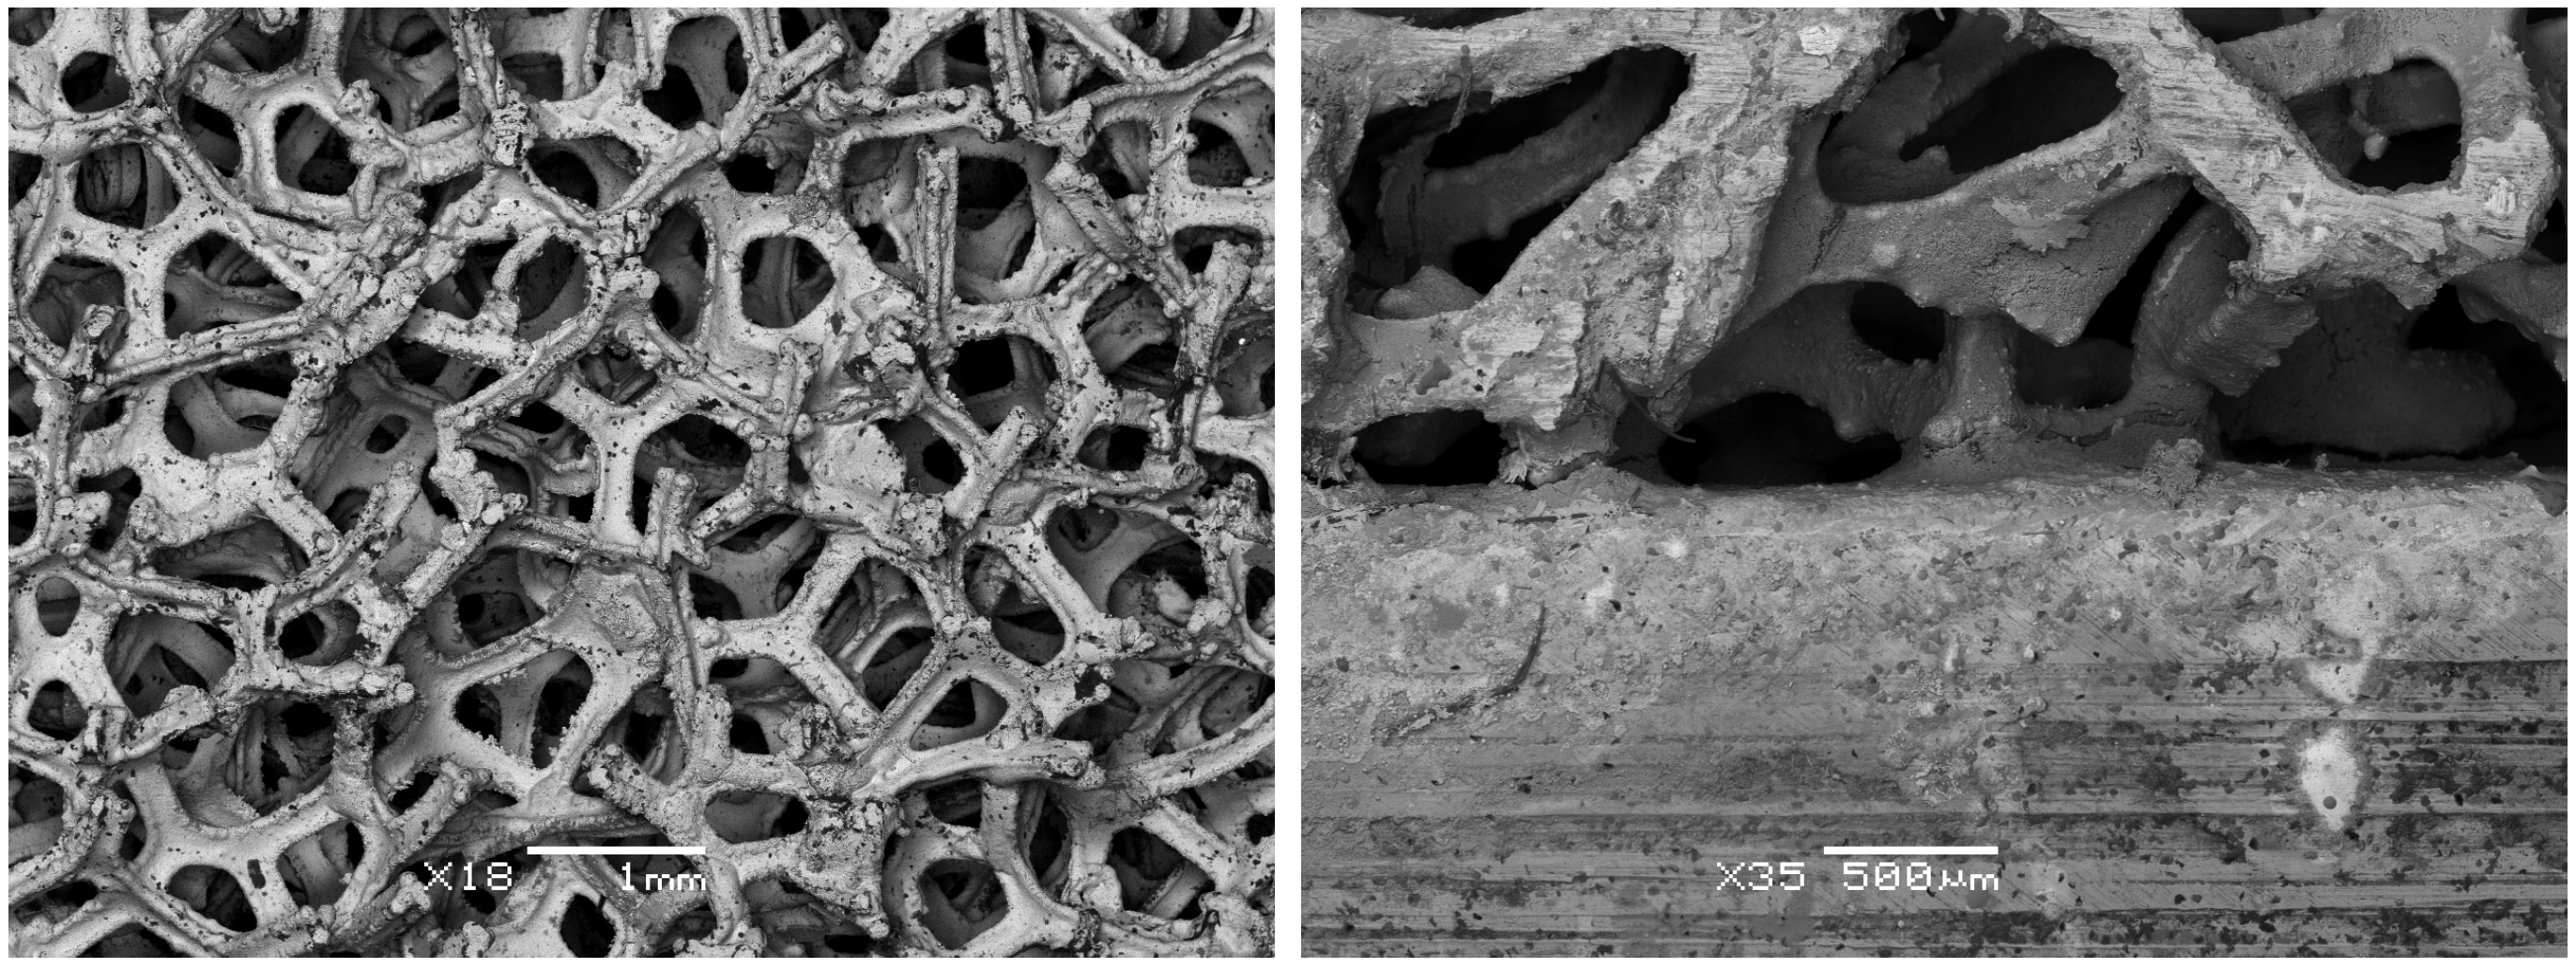
\includegraphics[width=14cm]{chf_3.png}
  \caption{Porous channel material after testing (left) and soldered joint (right).}
  \label{fig:provoz}
\end{figure}

Figure \ref{fig:chf_graf1} shows the experimental and numerical results of the pressure drop in the test section.
The numerical results match the experimental measurements for both samples.
The porous sample has a significantly higher pressure drop compared to the plain channel.
Figure \ref{fig:porous1} shows the static pressure contour of the porous channel sample.
Both pressure contours are for the case of 0.5~kg/s (30~L/min) of water mass flow.

\begin{figure}[ht!]
  \centering
  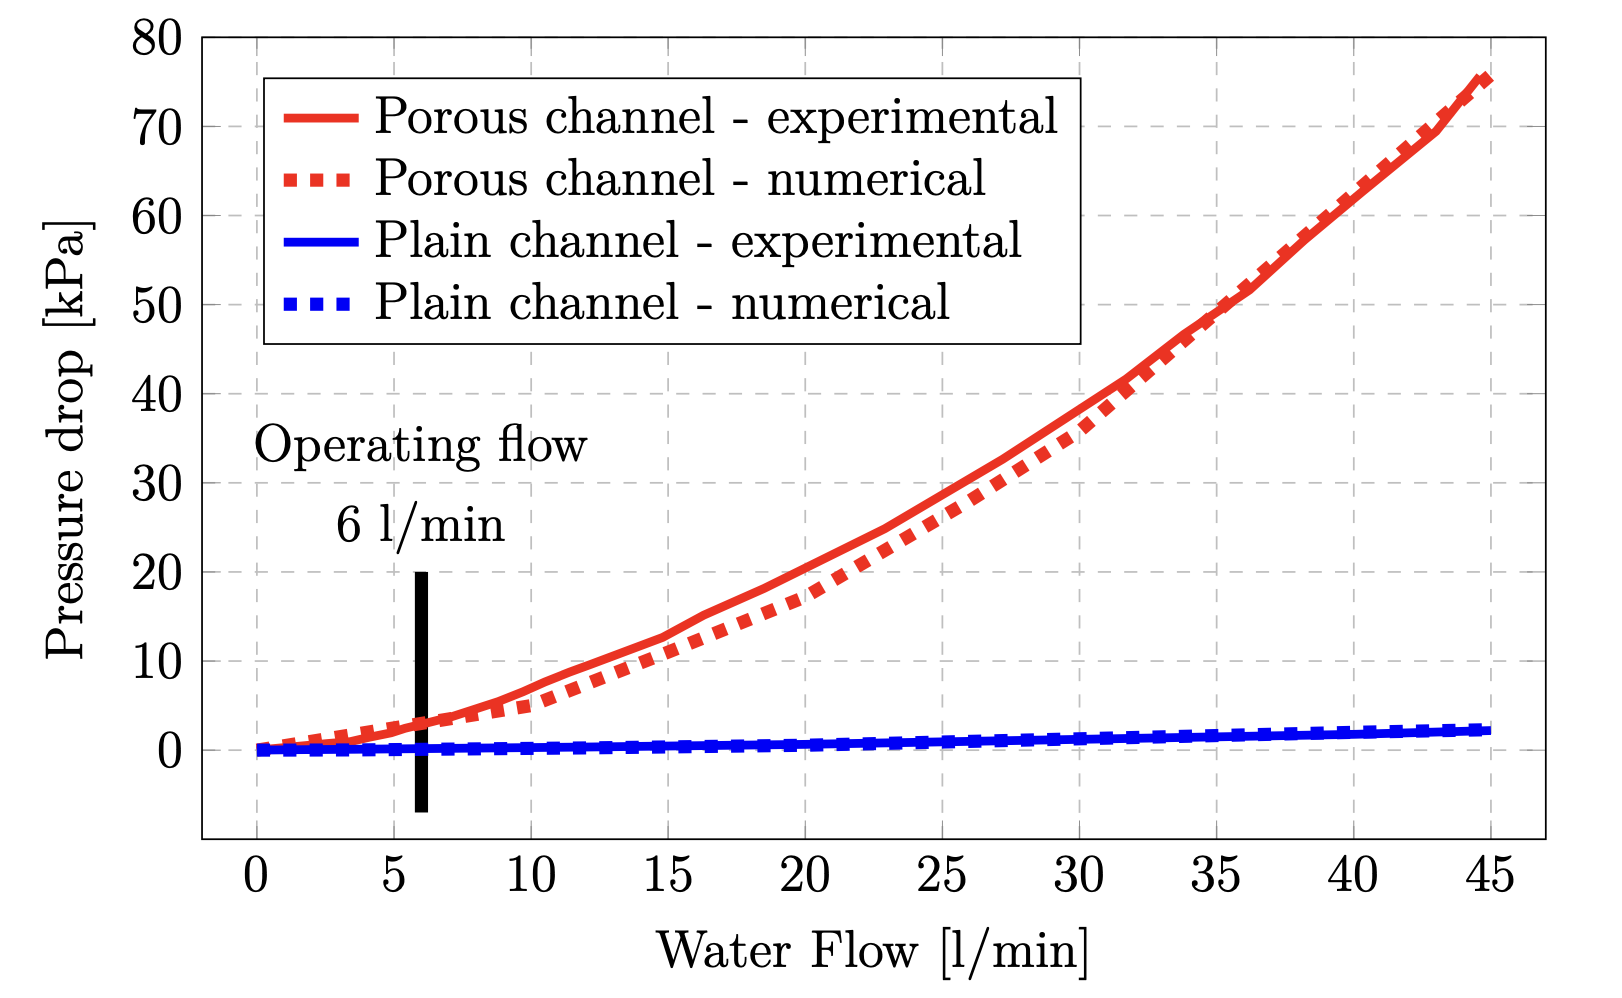
\includegraphics[width=10cm]{chf_5.png}
  \caption{The pressure drop of the experimental section.}
  \label{fig:chf_graf1}
\end{figure}

\pagebreak

\begin{figure}[ht!]
  \centering
  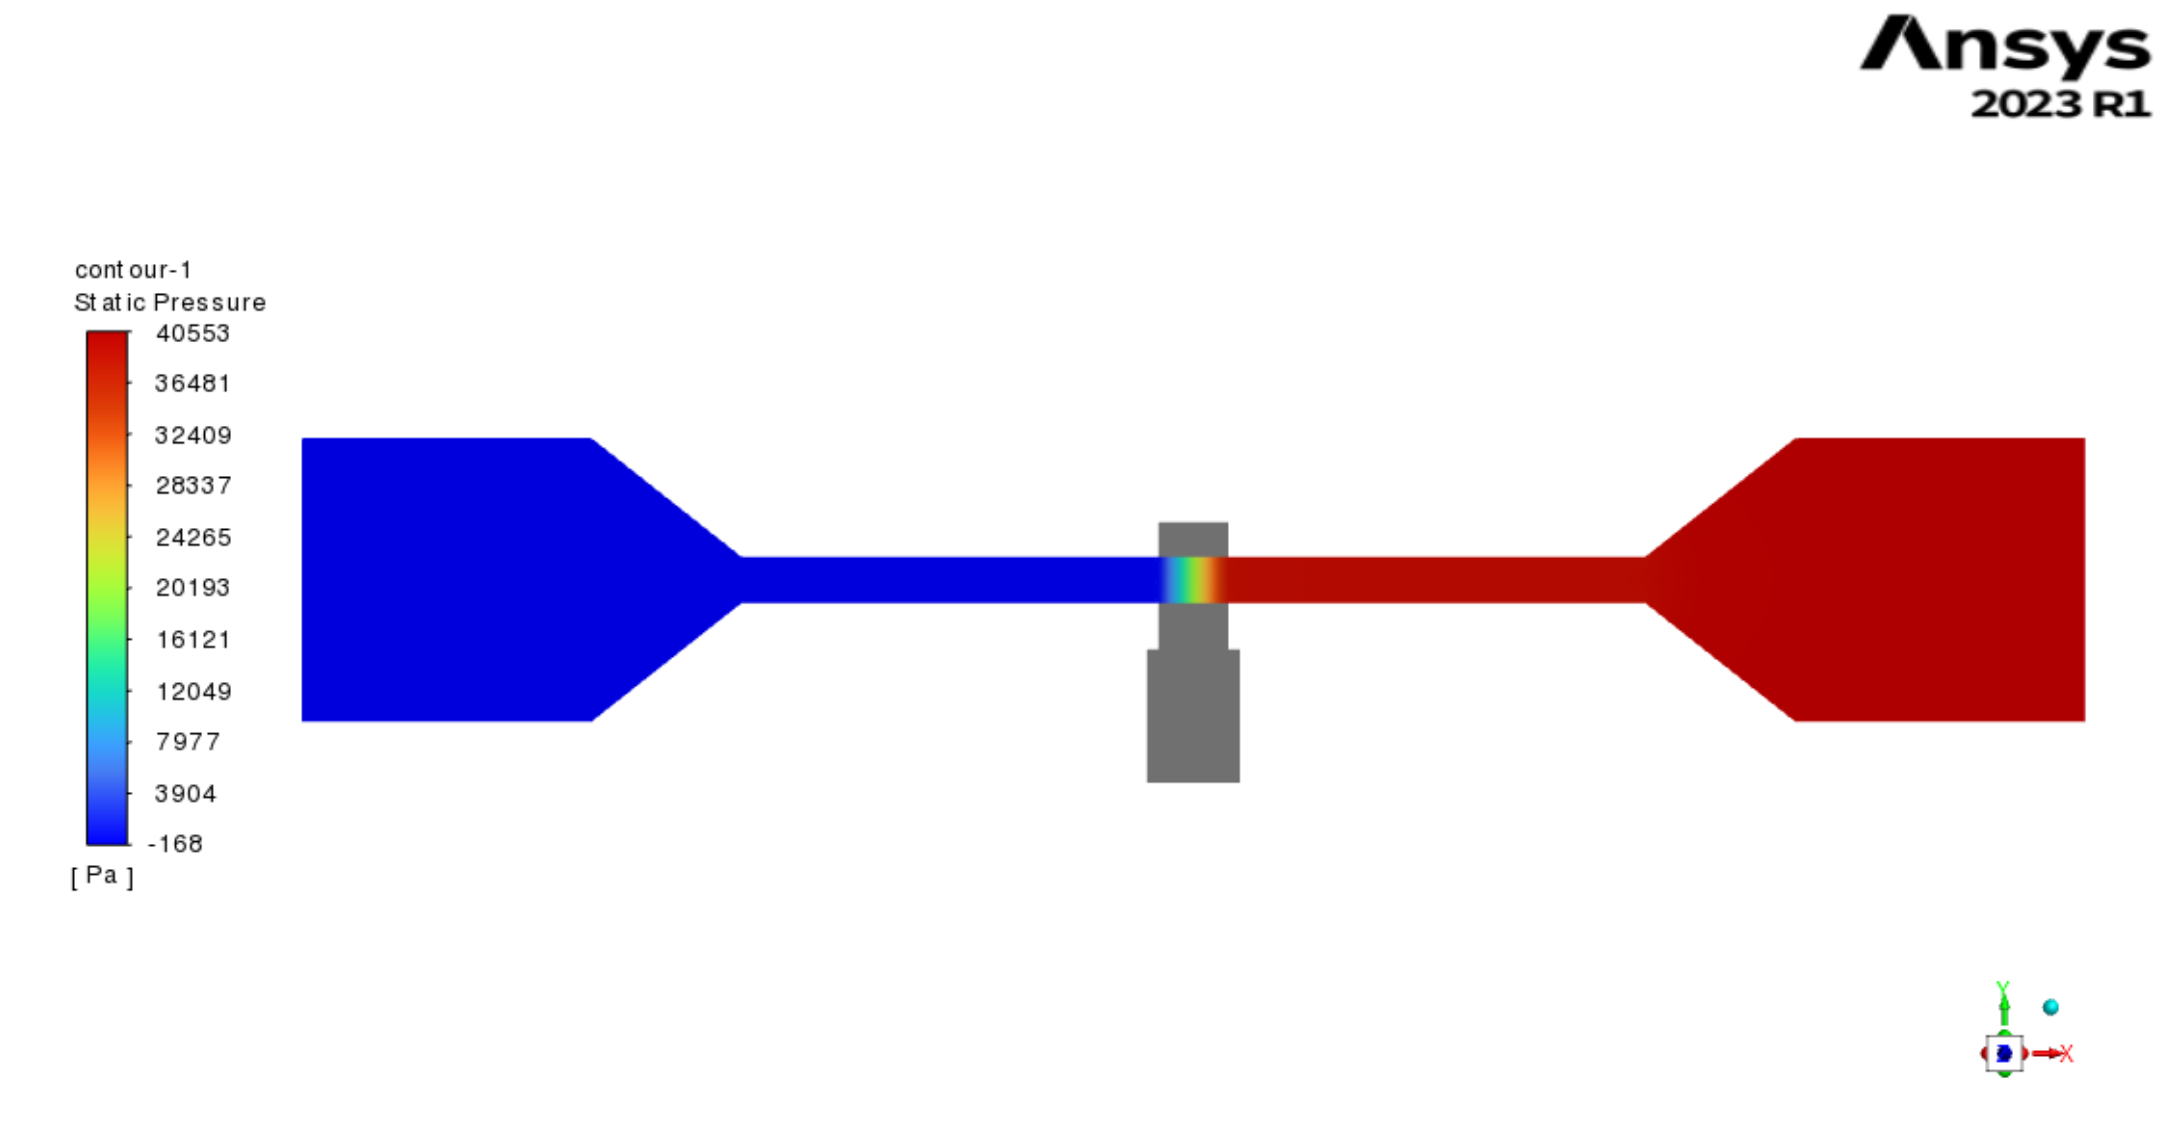
\includegraphics[width=14cm]{chf_6.png} 
  \caption{Plain channel - pressure contour, 0.5~kg/s water flow.}
  \label{fig:porous1}
\end{figure}

\subsubsection{Heat transfer and critical heat flux}

 Figure \ref{fig:chf_results} shows the experimental results of the thermocouple measurements at three different positions within the solid CuCrZr channel sample body.
The flow of the inlet water is 6~L/min, the inlet temperature is 60~$^\circ$C.
Increasing the heat flux on the tested samples resulted in various results.
The critical heat flux of the plain sample was observed at approximately 4~MW/m$^2$, a rapid increase of sample temperatures above this heat flux resulted in the termination of experimental measurements for safety reasons.
The porous sample was able to exhaust heat above this limit without a significant increase in temperature.
The experimental measurement of the porous sample was carried out up to 4.7~MW/m$^2$ due to the heating power limitations of the inductive heating source used.
Although the exact value of the critical heat flux value of the porous sample was not found, the results clearly indicate that the CHF value of the porous sample is significantly increased compared to that of the plain sample.

\begin{figure}[ht!]
  \centering
  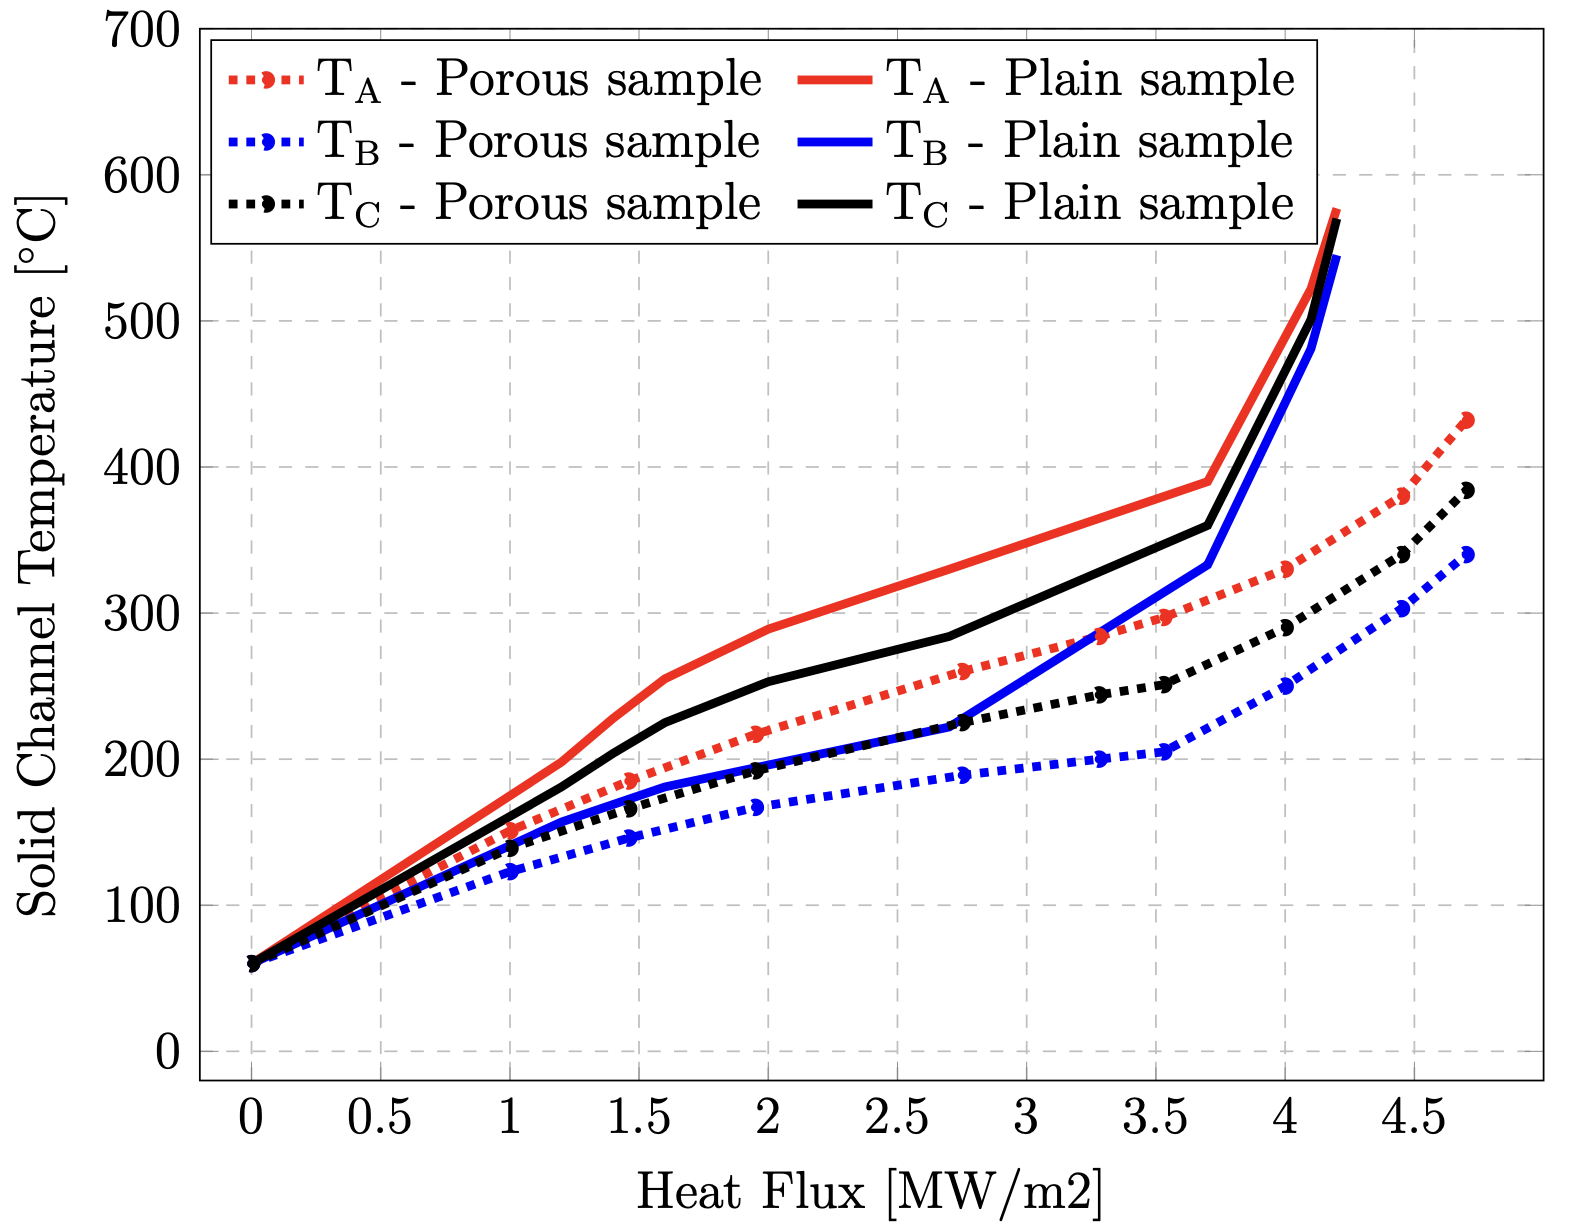
\includegraphics[width=14cm]{chf_8.png} 
  \caption{The heat transfer performance of tested samples.}
  \label{fig:chf_results}
\end{figure}

\subsubsection{Discussion}

The operating flow for heat transfer analysis measurements is set to a very low value of 6~L/min to achieve the critical heat flux on the plain sample and examine the difference between both samples in the perspective of the critical heat flux.
The CHF is the main focus of this research. 
The main purpose of the porous structure is to avoid the formation of a stable insulating vapor layer on the heated surface (the boiling crisis).
The microstructure of the porous material allows the capillary effect to deliver liquid water near the heated surface.
From this point of view, the conductivity of porous material is not only unnecessary but may also be unwanted.
\\
\\
Recent research on the Leidenfrost effect suggested a similar mechanism to prevent the formation of insulating vapor layer and also demonstrated the importance of low thermal conductivity of the porous material used \cite{Jiang2022}.
The present measurements therefore support the hypothesis that the porous insert delays dryout under the investigated conditions; however, the relative roles of capillary transport, pore size and solid thermal conductivity cannot be separated from this dataset alone.

\subsubsection{Conclusion of the proof of concept}
The design of the cooling channel based on porous copper material was introduced for high heat flux cooling applications.
The porous sample design was compared with the plain sample both experimentally and numerically.
A series of experimental analyses were conducted to evaluate the properties of microstructure porous materials: pore diameter, strut diameter, porosity, and chemical composition.
Empirical equations were used to evaluate the porous zone parameters for CFD analysis (Darcy--Forchheimer coefficients).
Numerical simulation of experimental test section with cooling channel samples was performed in ANSYS Fluent 2023 Release 1 for both porous sample and plain sample.
The pressure drop characteristics of the tested samples in the CFD analysis match the experimental data.
\\
\\
Experimental measurements of heat transfer of both samples resulted in various results.
The plain sample reached critical heat flux at approximately 4~MW/m$^2$, whereas critical heat flux was not reached for the porous sample within the available heating-power range.
Within the investigated boundary conditions, the porous insert therefore increased the demonstrated CHF margin relative to the plain channel, although the absolute CHF of the porous configuration remains above the maximum heat flux reached in the experiment.

\pagebreak
\section{Summary}
The original work combines numerical modelling and experimental measurements at three levels of geometrical fidelity. First, a controlled family of substitute porous geometries was used to isolate the influence of porosity and tortuosity on hydraulic resistance. The simulations showed that permeability increases strongly with porosity and decreases with tortuosity, while the inertial contribution represented by the Forchheimer coefficient follows the opposite tendency. The numerical methodology was validated against additively manufactured reference samples, with the predicted pressure losses generally agreeing with the measurements within approximately 10\,\% over most of the investigated range.

Second, commercially available porous samples were characterized experimentally. Microscopy and hydraulic measurements confirmed that nominal descriptors such as PPI or porosity alone are insufficient to predict the pressure loss of real porous materials. Samples with apparently similar nominal properties can exhibit substantially different hydraulic behaviour because of differences in pore connectivity, strut morphology and tortuosity. The fitted Darcy--Forchheimer coefficients therefore provide a more useful engineering description of the tested materials than a single manufacturer-specified microstructural parameter.

Third, realistic structures reconstructed from micro-computed tomography were analysed numerically. The microCT models reproduced the measured hydraulic behaviour and enabled conjugate heat-transfer calculations inside the actual porous geometry. The comparison of copper, tin and alumina matrices demonstrated the strong role of solid thermal conductivity in distributing heat away from the loaded surface: copper provided the most effective lateral heat spreading, whereas lower-conductivity materials confined the thermal field closer to the heated region.

Finally, the proof-of-concept high-heat-flux experiment compared a plain CuCrZr channel with a channel containing a porous copper insert. The plain channel reached boiling crisis at approximately 4~MW/m$^2$. The porous configuration remained stable up to the maximum experimentally available heat flux of 4.7~MW/m$^2$, at which the heater power limit was reached before CHF occurred. The experiment therefore demonstrates an increased CHF margin for the porous configuration under the investigated conditions, while not determining its absolute CHF.

Taken together, the results show that porous cooling structures can provide substantial thermal benefits, but these benefits are inseparable from increased and strongly microstructure-dependent hydraulic resistance. A reliable design procedure must therefore combine geometric characterization, pressure-loss measurement or validated CFD, and thermal analysis rather than relying on porosity or PPI alone.

\pagebreak

\part{Conclusion}
The objective of this dissertation was to characterize the thermohydraulic behaviour of porous cooling structures and to determine which microstructural parameters control their hydraulic and thermal performance under conditions relevant to high-heat-flux fusion applications. This objective was addressed through a combination of controlled substitute geometries, experimental hydraulic characterization, microCT-based CFD and a proof-of-concept CHF experiment.

\textbf{H1: Hydraulic resistance.} The hypothesis is supported within the investigated parameter range. Porous inserts introduce substantially higher pressure losses than smooth channels, but the losses can be described using Darcy--Forchheimer coefficients and varied systematically through the geometry. The parametric study demonstrated that increasing porosity reduces hydraulic resistance, whereas increasing tortuosity increases it. Hydraulic loss is therefore an important design constraint, but not an intrinsically prohibitive one when the geometry and operating point are selected together.

\textbf{H2: Relation between microstructure and hydraulic behaviour.} The hypothesis is partially confirmed and requires an important qualification. For the controlled substitute geometries, clear quantitative relationships between porosity, tortuosity, permeability and inertial losses were obtained. For real commercial foams, however, microscopy showed that porosity and PPI alone do not uniquely determine hydraulic behaviour. Reliable prediction requires additional information describing pore connectivity, strut geometry and tortuosity, or direct calibration against hydraulic data. This distinction is one of the principal outcomes of the work.

\textbf{H3: Enhancement of critical heat flux.} The proof-of-concept experiment supports the hypothesis qualitatively but does not establish the absolute CHF of the porous configuration. The plain channel reached CHF at approximately 4~MW/m$^2$, while the porous sample remained thermally stable up to 4.7~MW/m$^2$, where the available induction-heating power became the limiting factor. The observed result is consistent with enhanced liquid redistribution and rewetting in the porous structure, but the present measurements do not allow the individual contributions of capillarity, mixing and solid thermal conductivity to be separated.

The dissertation therefore demonstrates that porous materials are a technically credible route for extending the operating envelope of water-cooled high-heat-flux components. Their principal advantage is not simply the additional internal surface area, but the possibility of tailoring both liquid transport and heat spreading through the microstructure. At the same time, the work shows why a universal porous-medium correlation is unlikely to be sufficient for engineering design: realistic structures must be characterized at a level that captures the geometry responsible for both viscous and inertial losses. The validated numerical and experimental methods developed here provide such a framework.

\pagebreak

\part{Bibliography}
\printbibliography[filter=otherrefs,title={References},resetnumbers=true]
\pagebreak

\AtNextBibliography{\defcounter{maxnames}{99}\defcounter{minnames}{99}}
\printbibliography[filter=mypubs,title={Publications of the Author},resetnumbers=true]

\pagebreak
\listoffigures
\listoftables
\newpage
\pagenumbering{arabic}

\clearpage
\part{Appendices}

\section*{Appendix A -- Substitute Porous Structure -- All Results}

This appendix presents the complete set of results discussed in Chapter 10, \textit{The Use of Substitute Geometries and Accuracy of CFD}. While the main chapter focuses on the most representative findings and their interpretation, the full collection of numerical results is provided here for completeness and transparency. These data support the analyses presented in Chapter 10 and allow a comprehensive assessment of the accuracy and applicability of the investigated substitute geometries.

\begin{figure}[htbp]
  \centering
  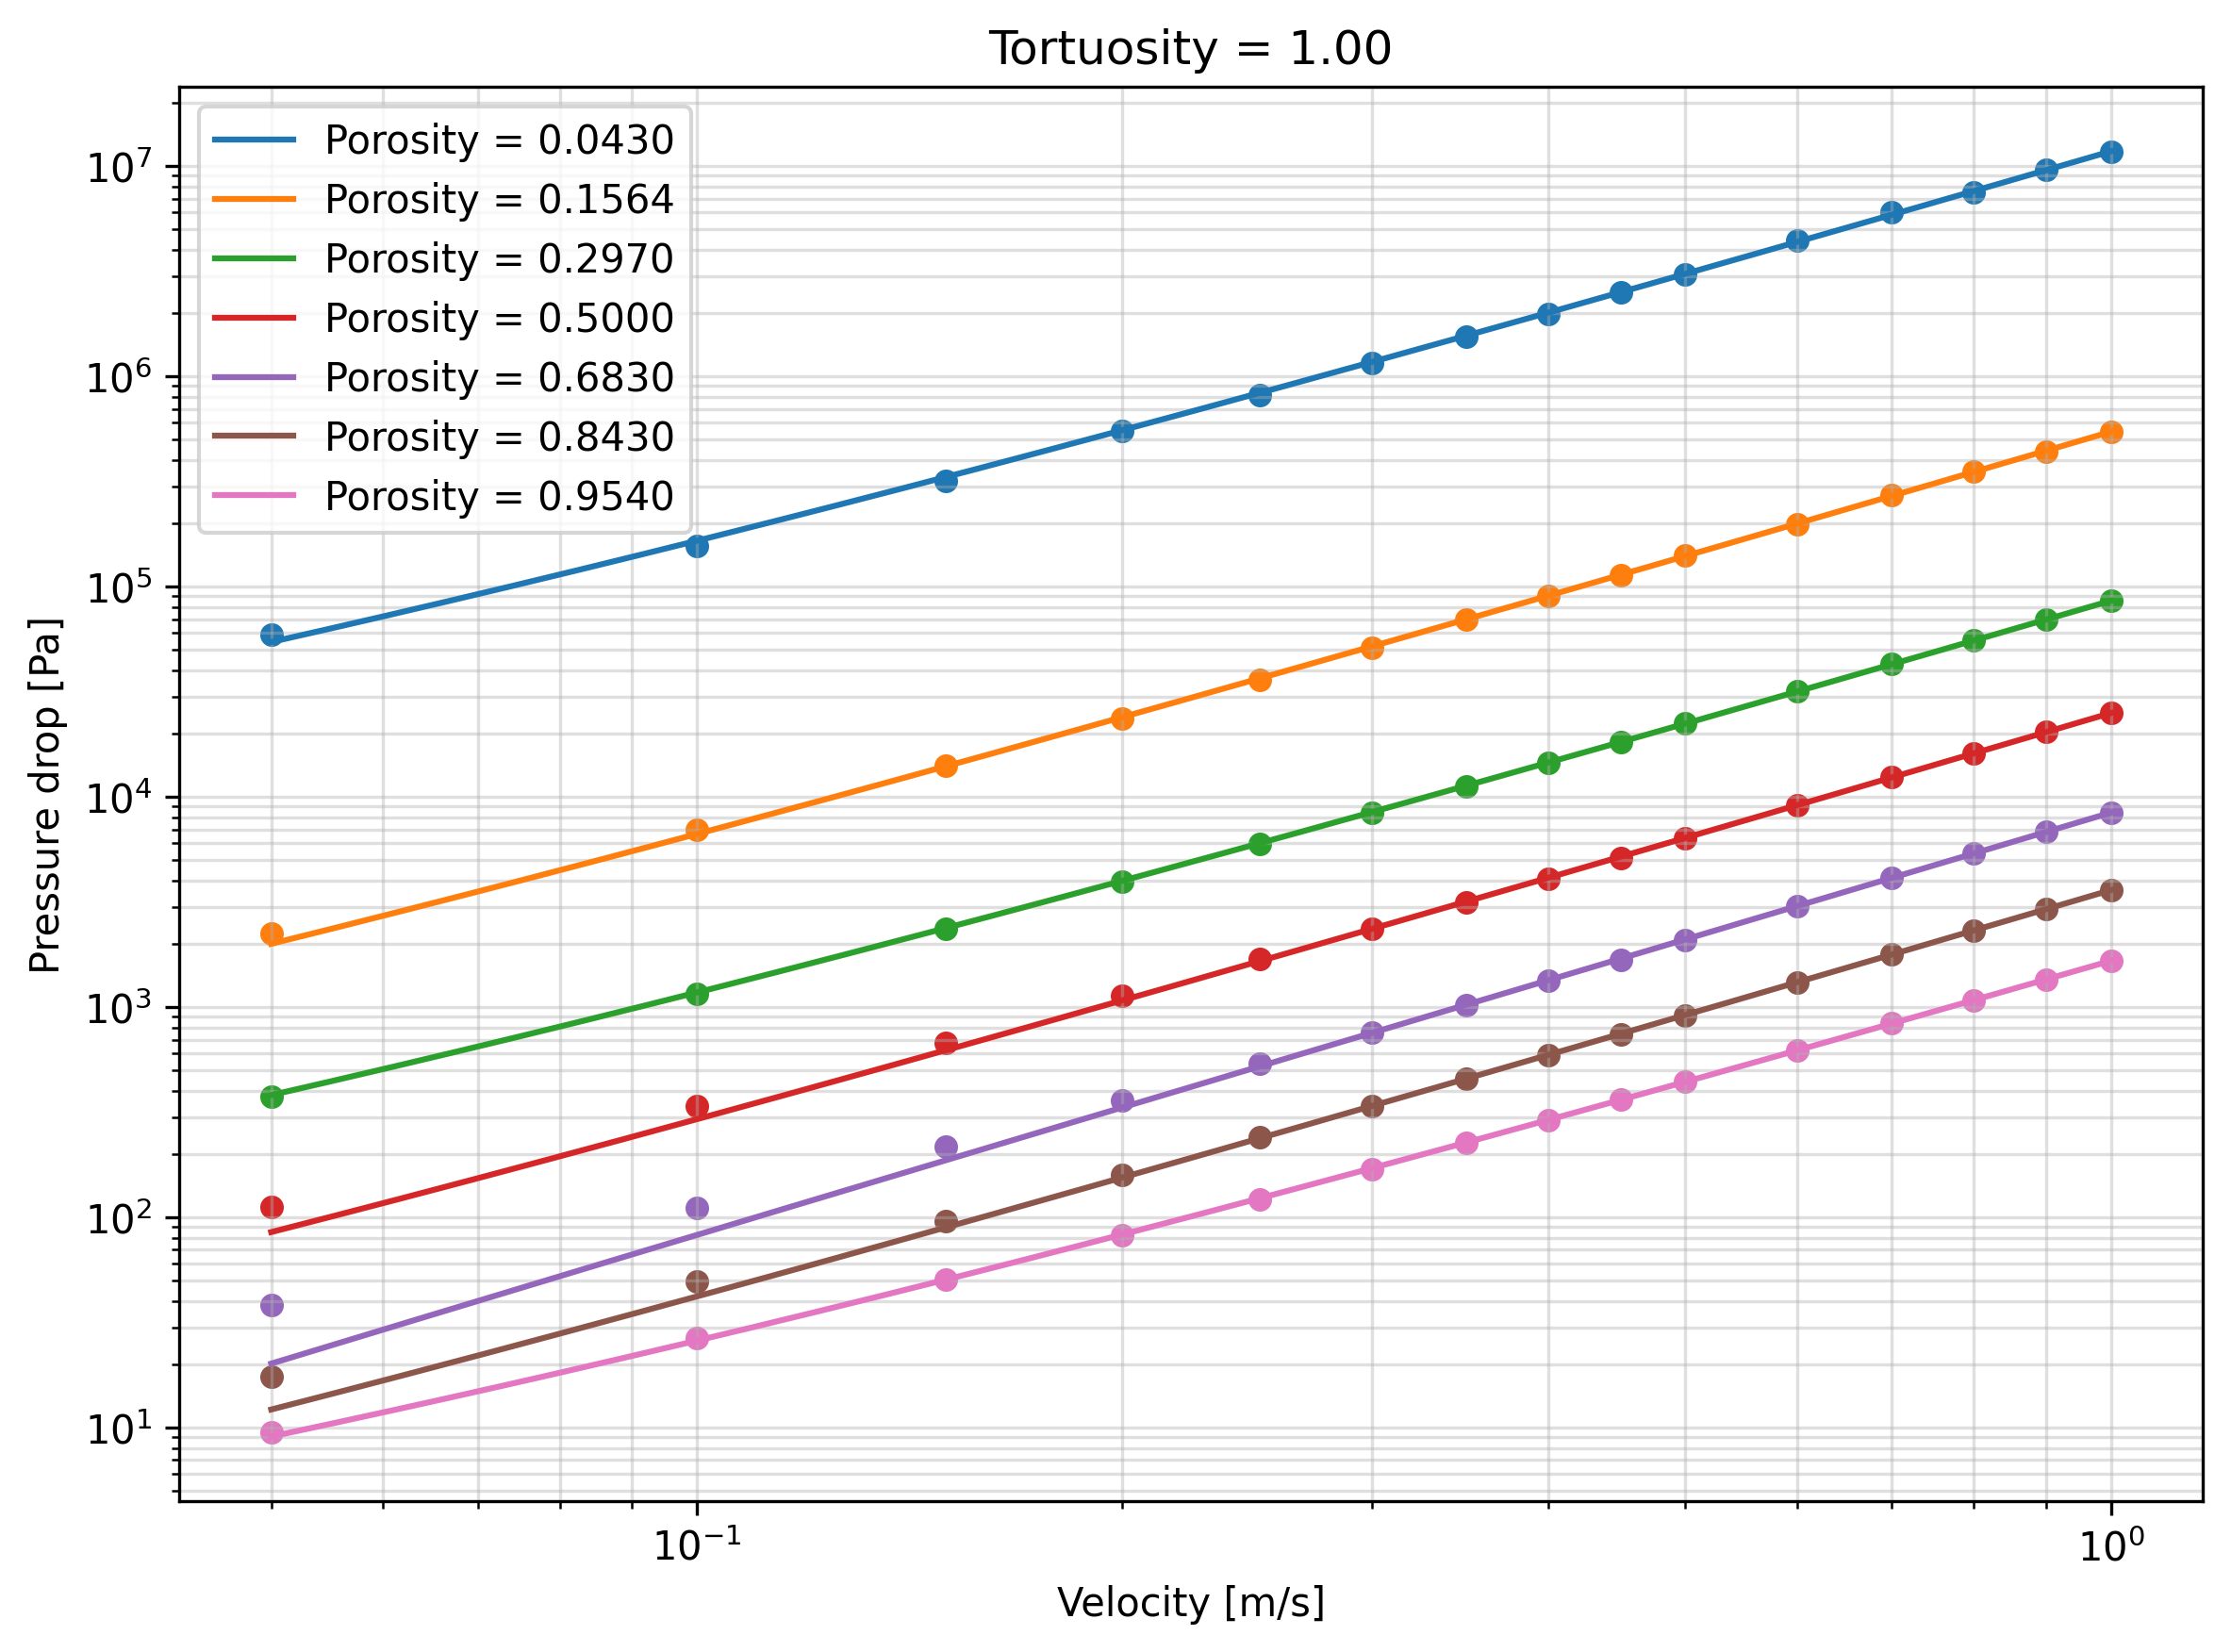
\includegraphics[width=14cm]{gr_tor1.png}
  \caption{Resulting pressure-drop characteristics for a tortuosity of 1.}
\end{figure}

\begin{figure}[htbp]
  \centering
  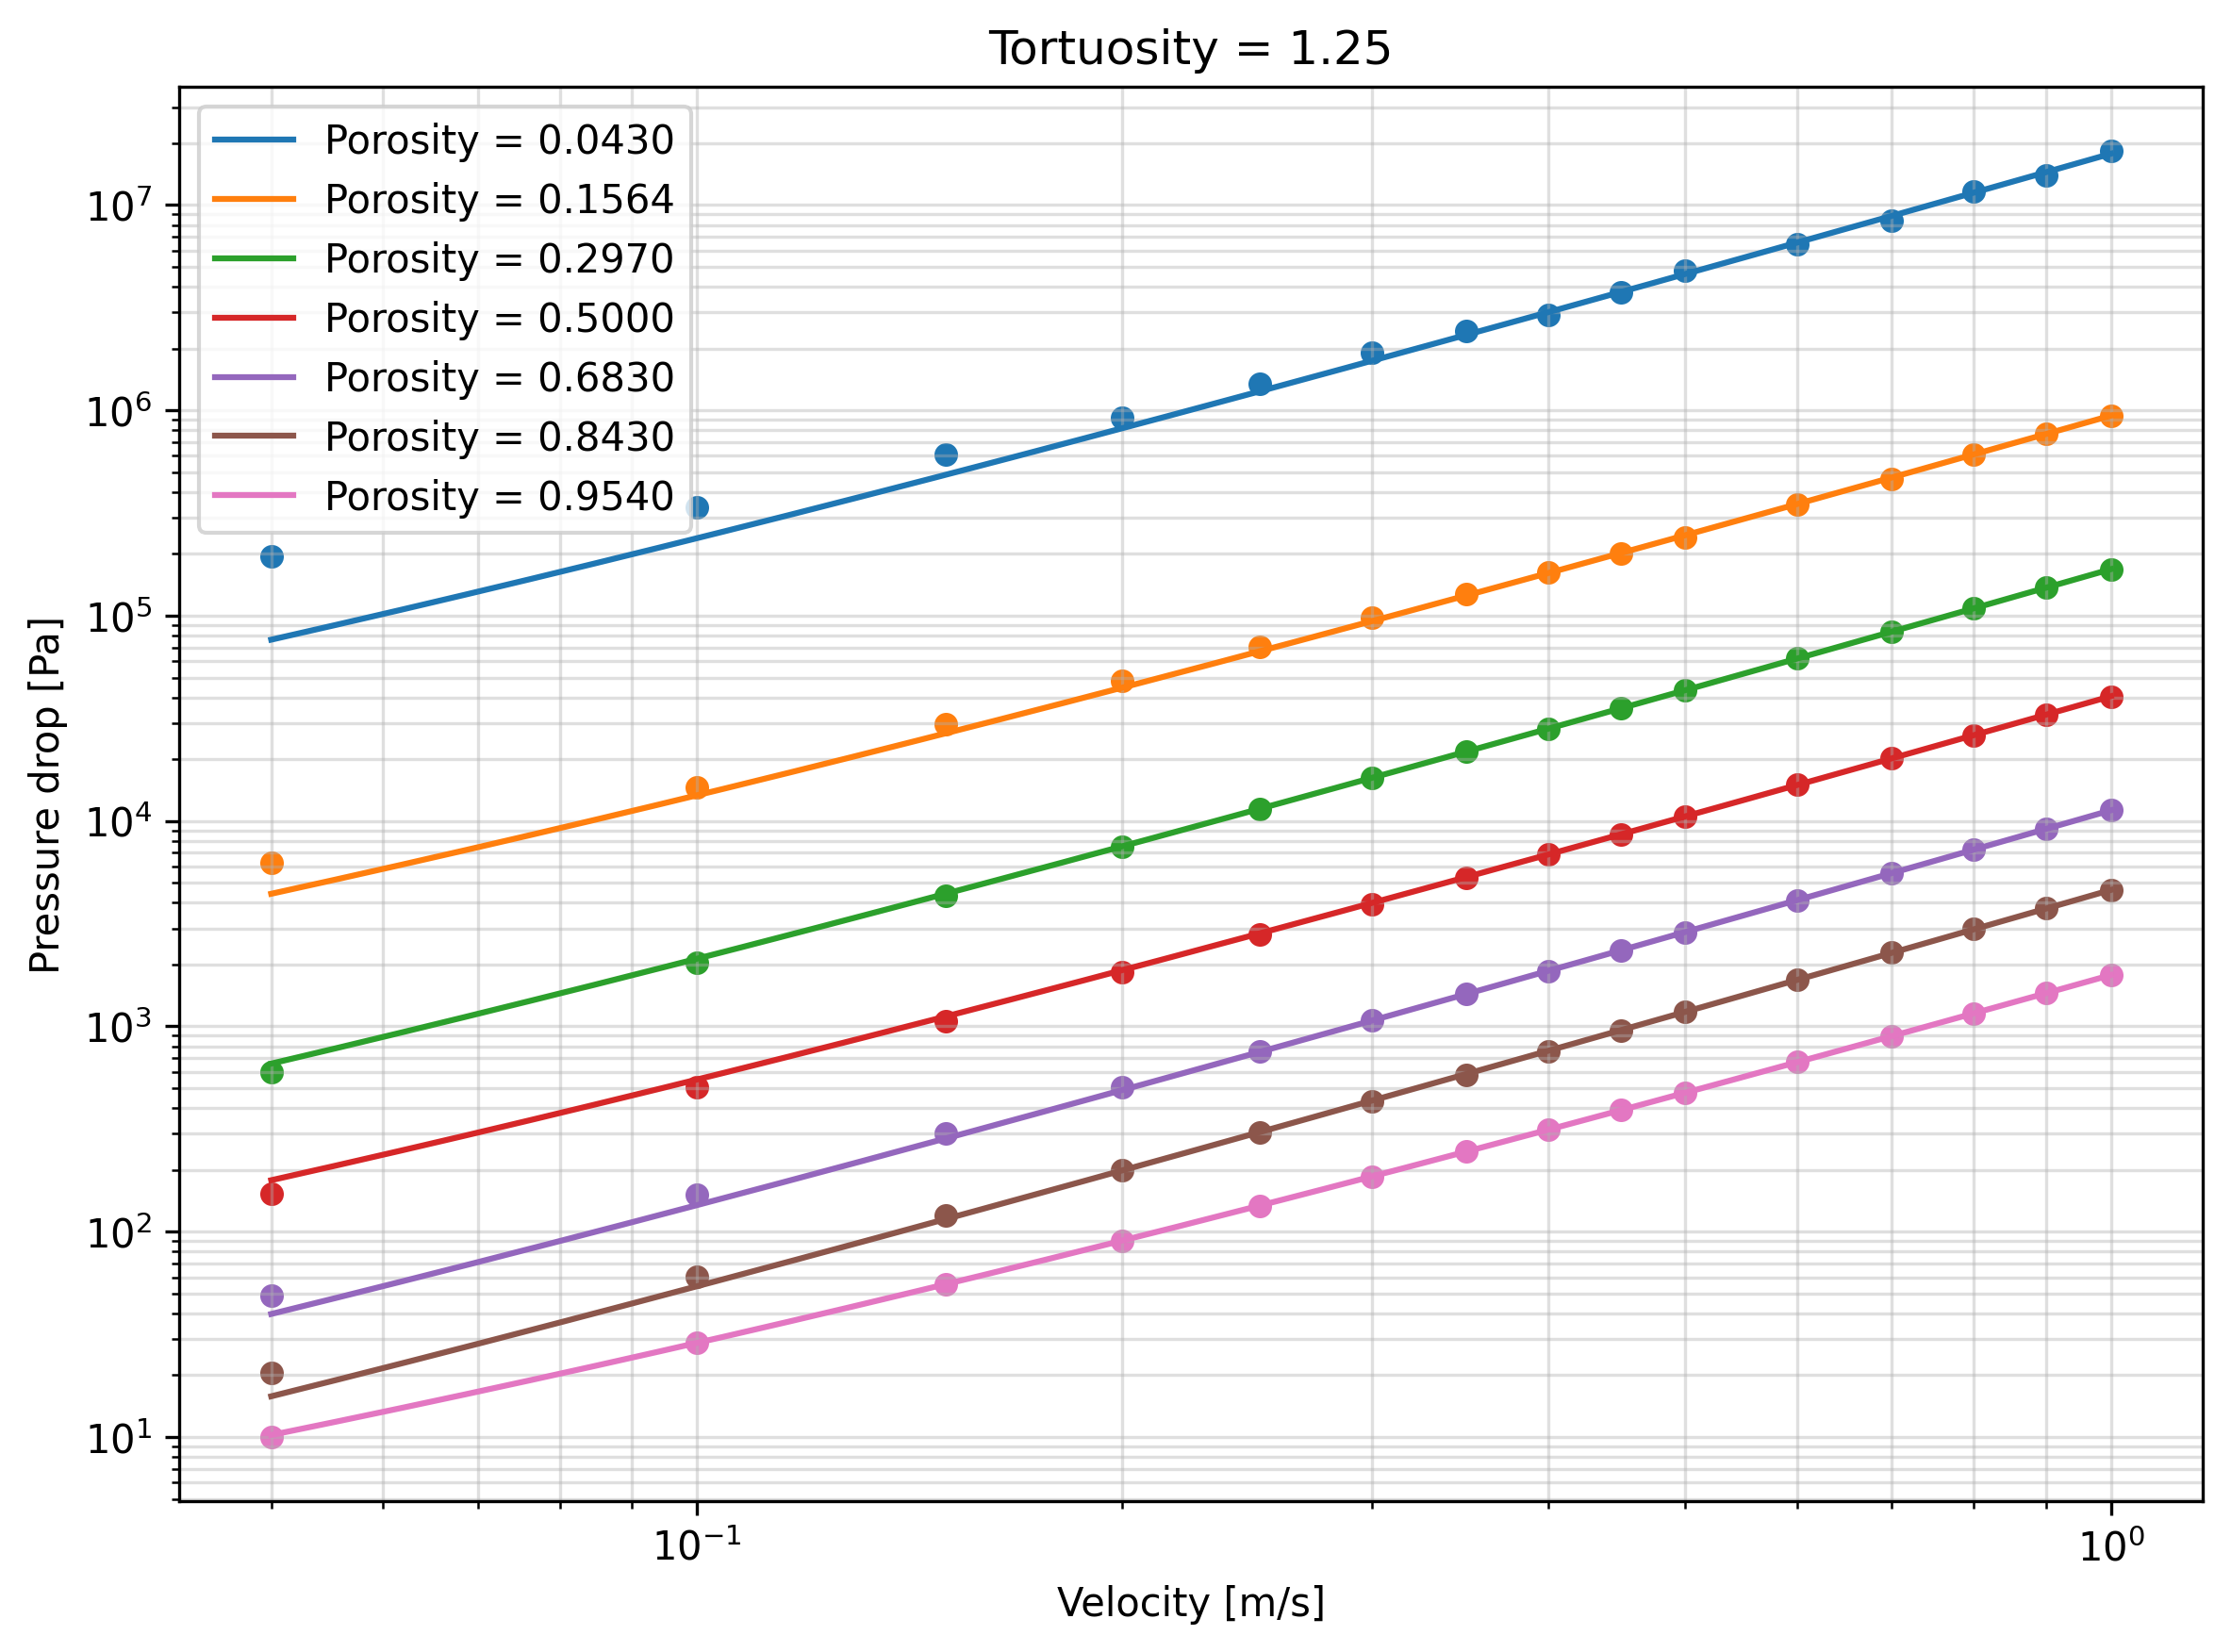
\includegraphics[width=14cm]{gr_tor125.png}
  \caption{Resulting pressure-drop characteristics for a tortuosity of 1.25.}
\end{figure}

\begin{figure}[htbp]
  \centering
  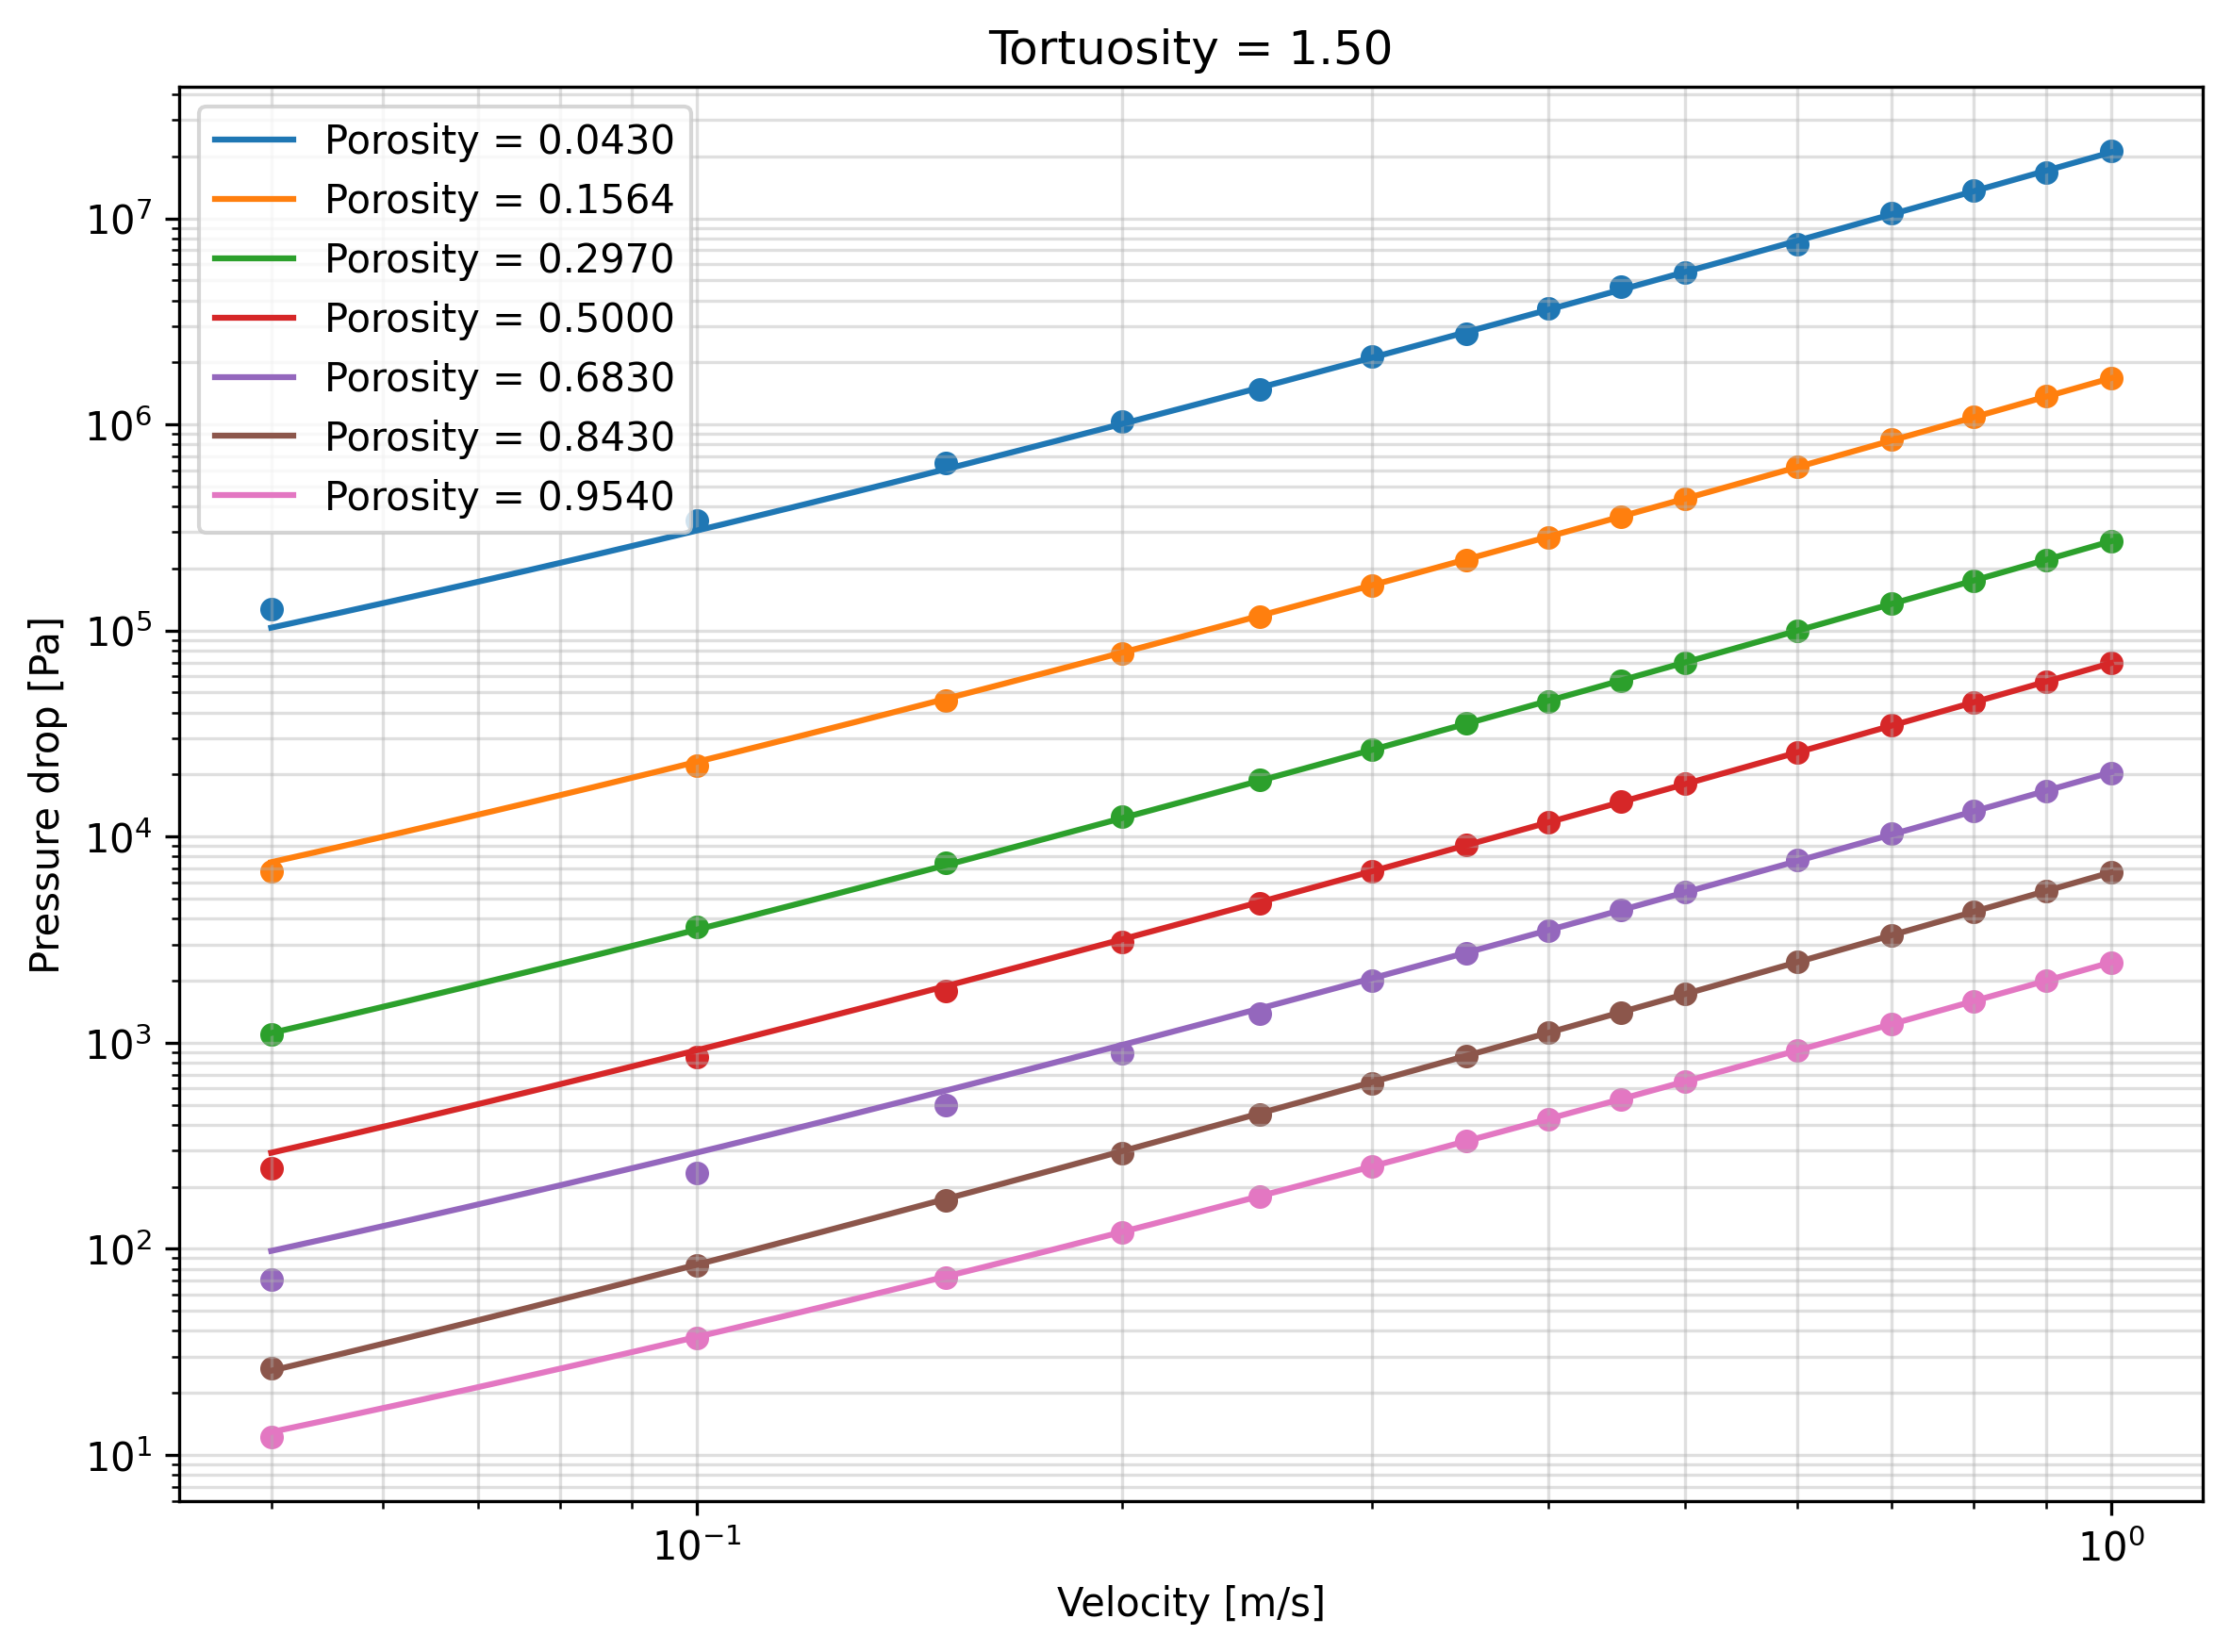
\includegraphics[width=14cm]{gr_tor15.png}
  \caption{Resulting pressure-drop characteristics for a tortuosity of 1.5.}
\end{figure}

\begin{figure}[htbp]
  \centering
  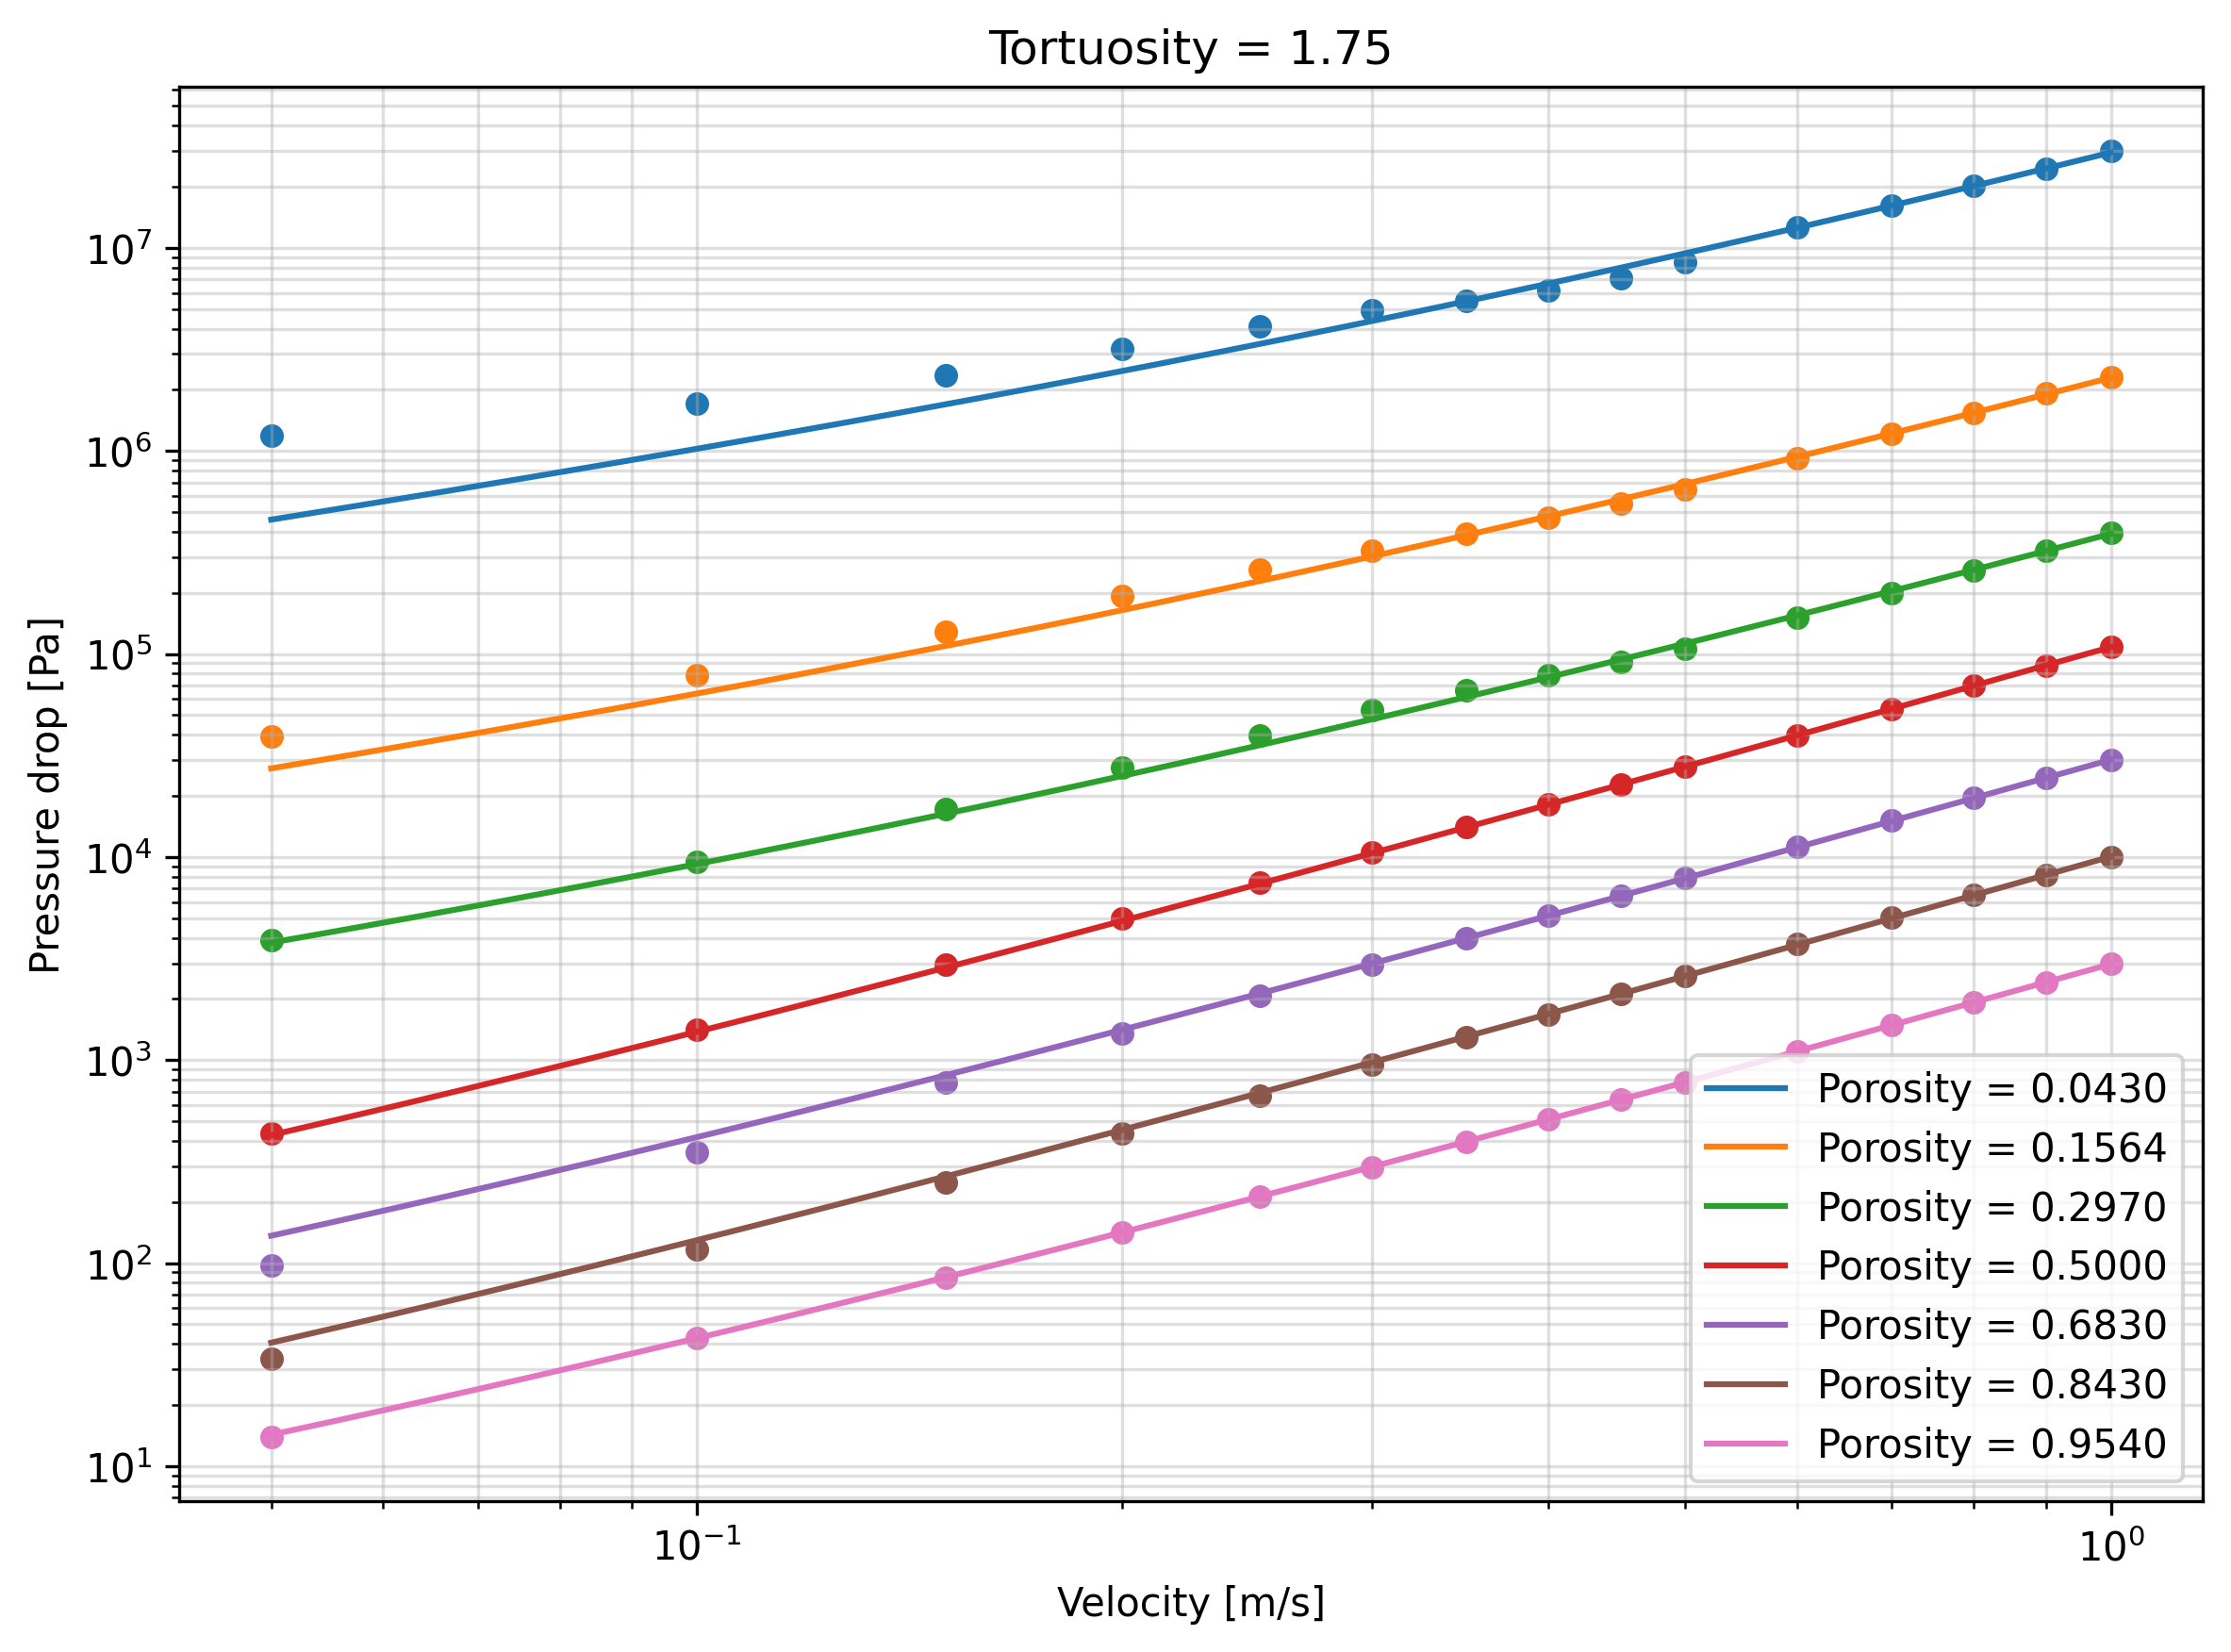
\includegraphics[width=14cm]{gr_tor175.png}
  \caption{Resulting pressure-drop characteristics for a tortuosity of 1.75.}
\end{figure}

\begin{figure}[htbp]
  \centering
  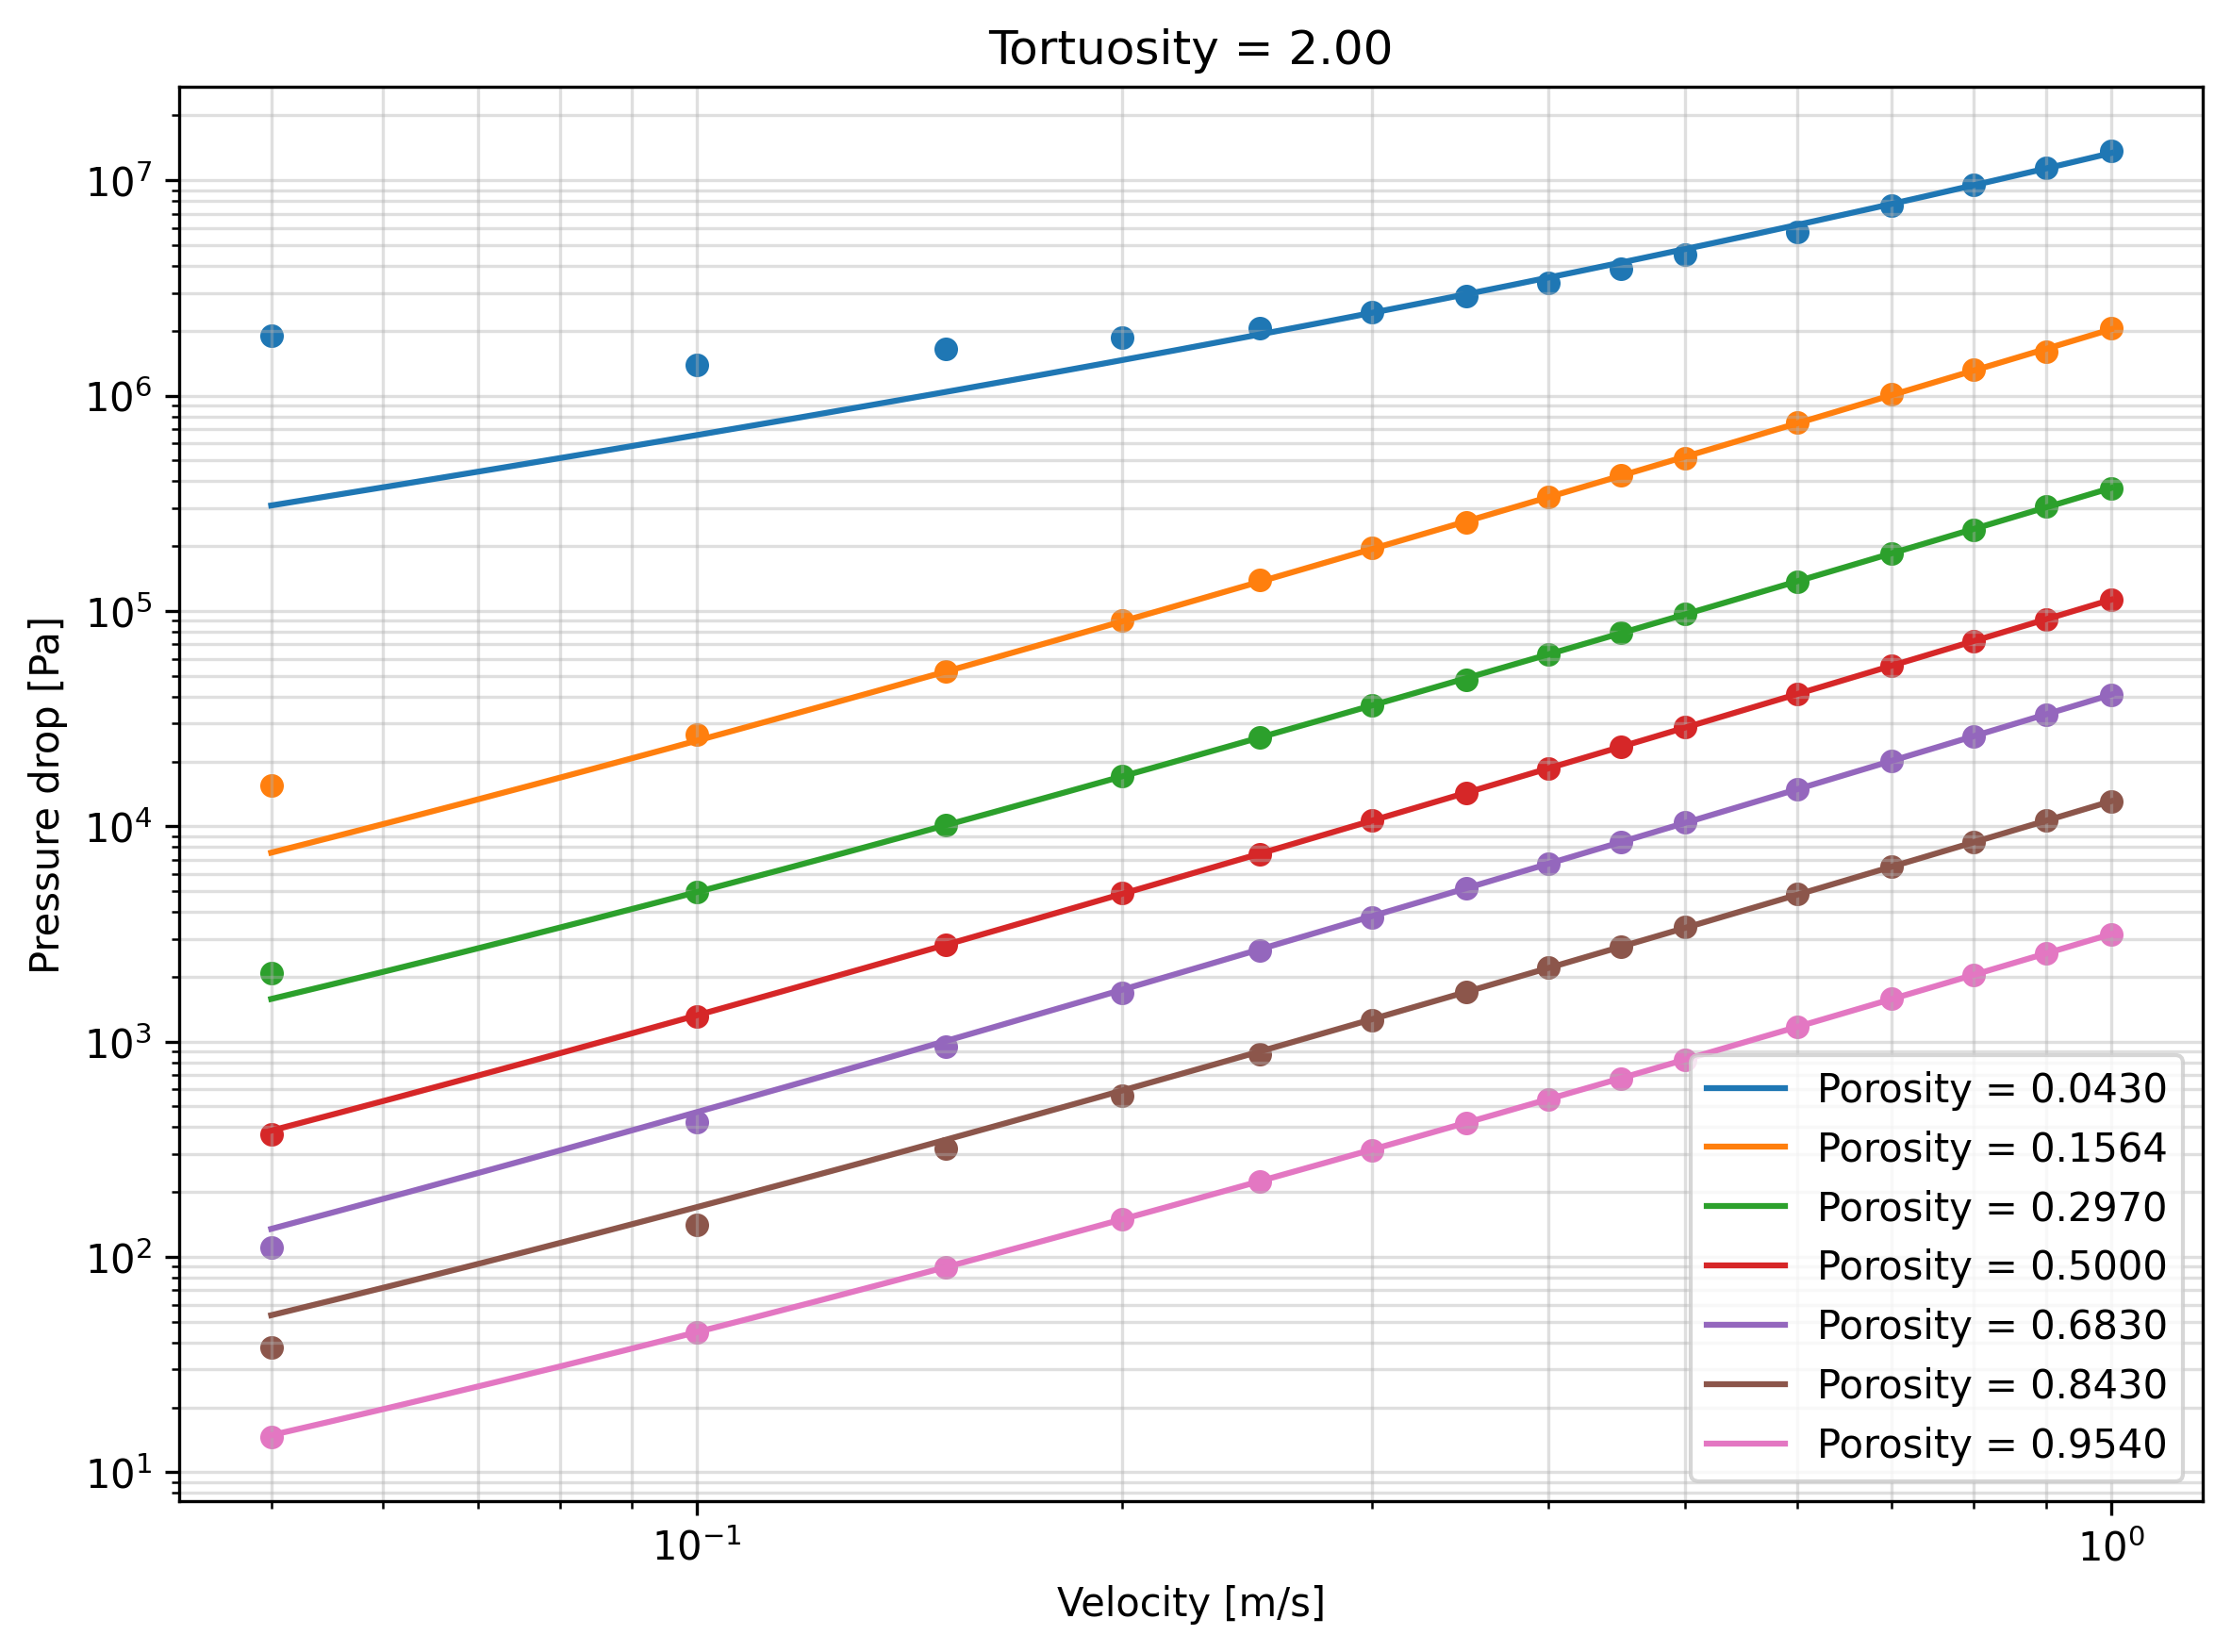
\includegraphics[width=14cm]{gr_tor2.png}
  \caption{Resulting pressure-drop characteristics for a tortuosity of 2.}
\end{figure}

% Vysází všechny čekající obrázky z Appendix A
% a teprve potom začne Appendix B.
\clearpage

\section*{Appendix B -- Experimental Measurements -- All Results}

This appendix presents the complete experimental results for the porous material samples investigated in Chapter 11. The full pressure-drop characteristics of all sample groups are provided to complement the analysis and discussion presented in the main text.

\begin{figure}[htbp]
  \centering
  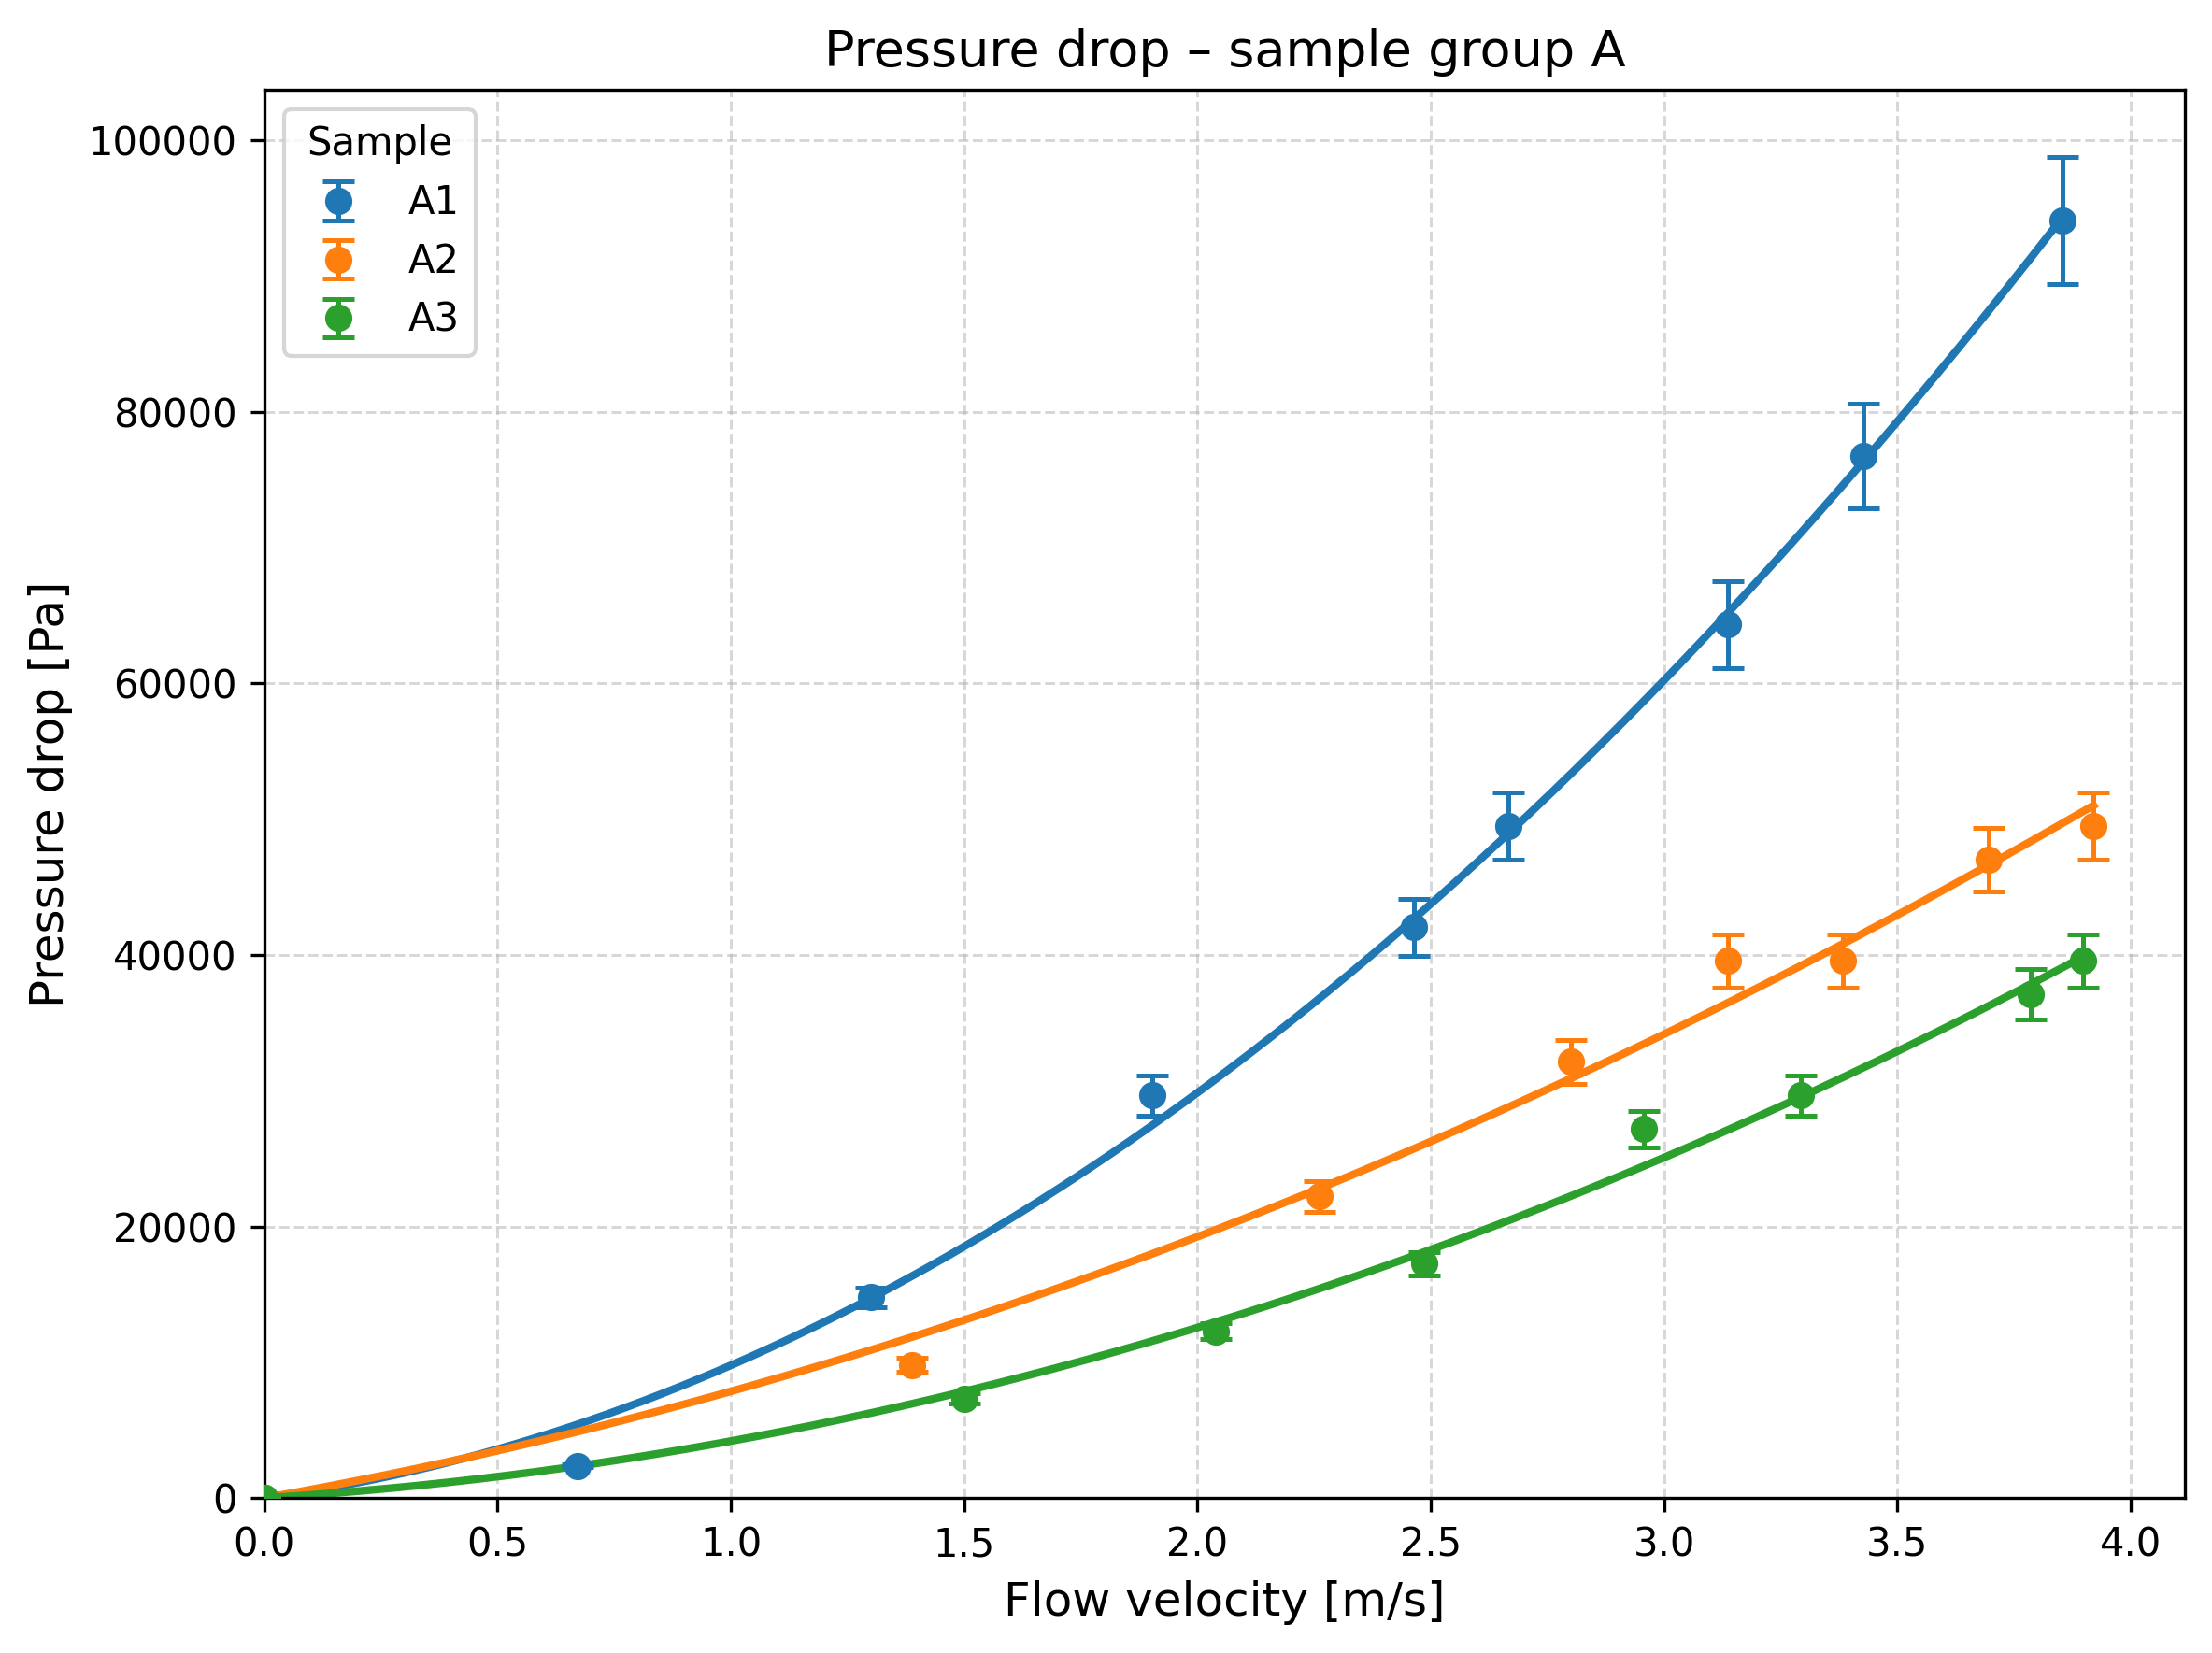
\includegraphics[width=10cm]{group_A_pressure_drop_velocity.png}
  \caption{Pressure drop across the porous zone for sample set A.}
  \label{fig:appendix_foam_results_A}
\end{figure}

\begin{figure}[htbp]
  \centering
  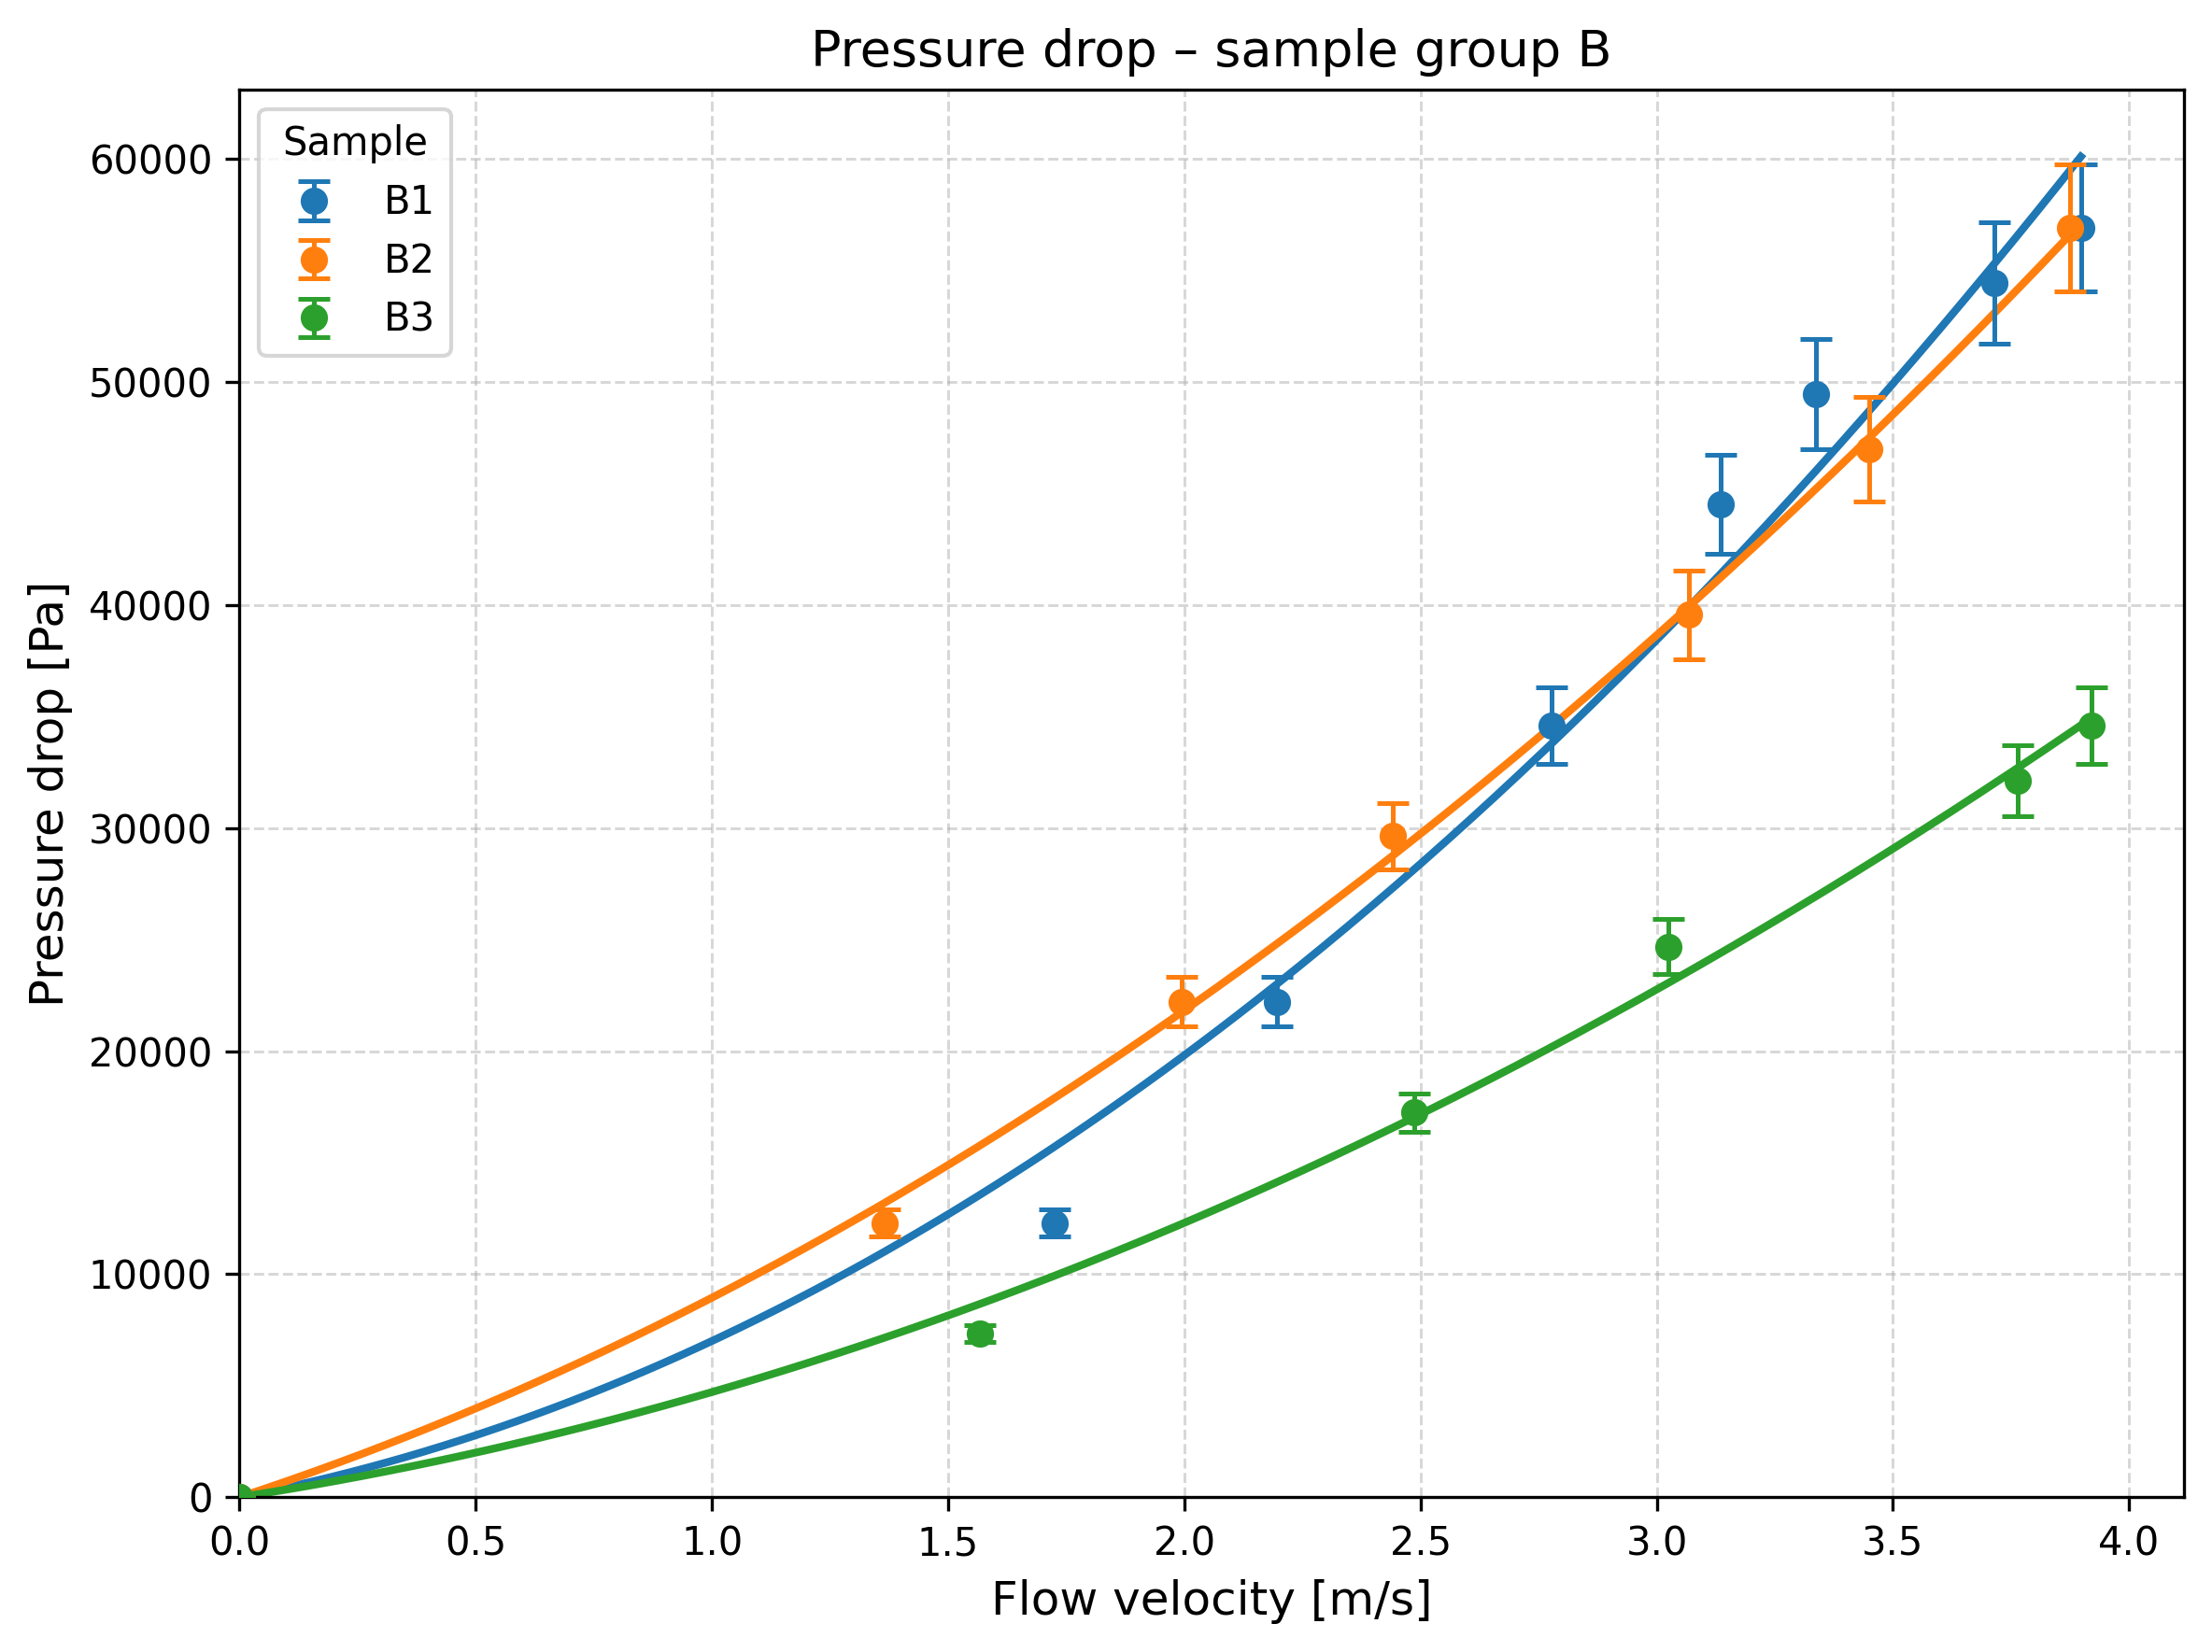
\includegraphics[width=10cm]{group_B_pressure_drop_velocity.png}
  \caption{Pressure drop across the porous zone for sample set B.}
\end{figure}

\begin{figure}[htbp]
  \centering
  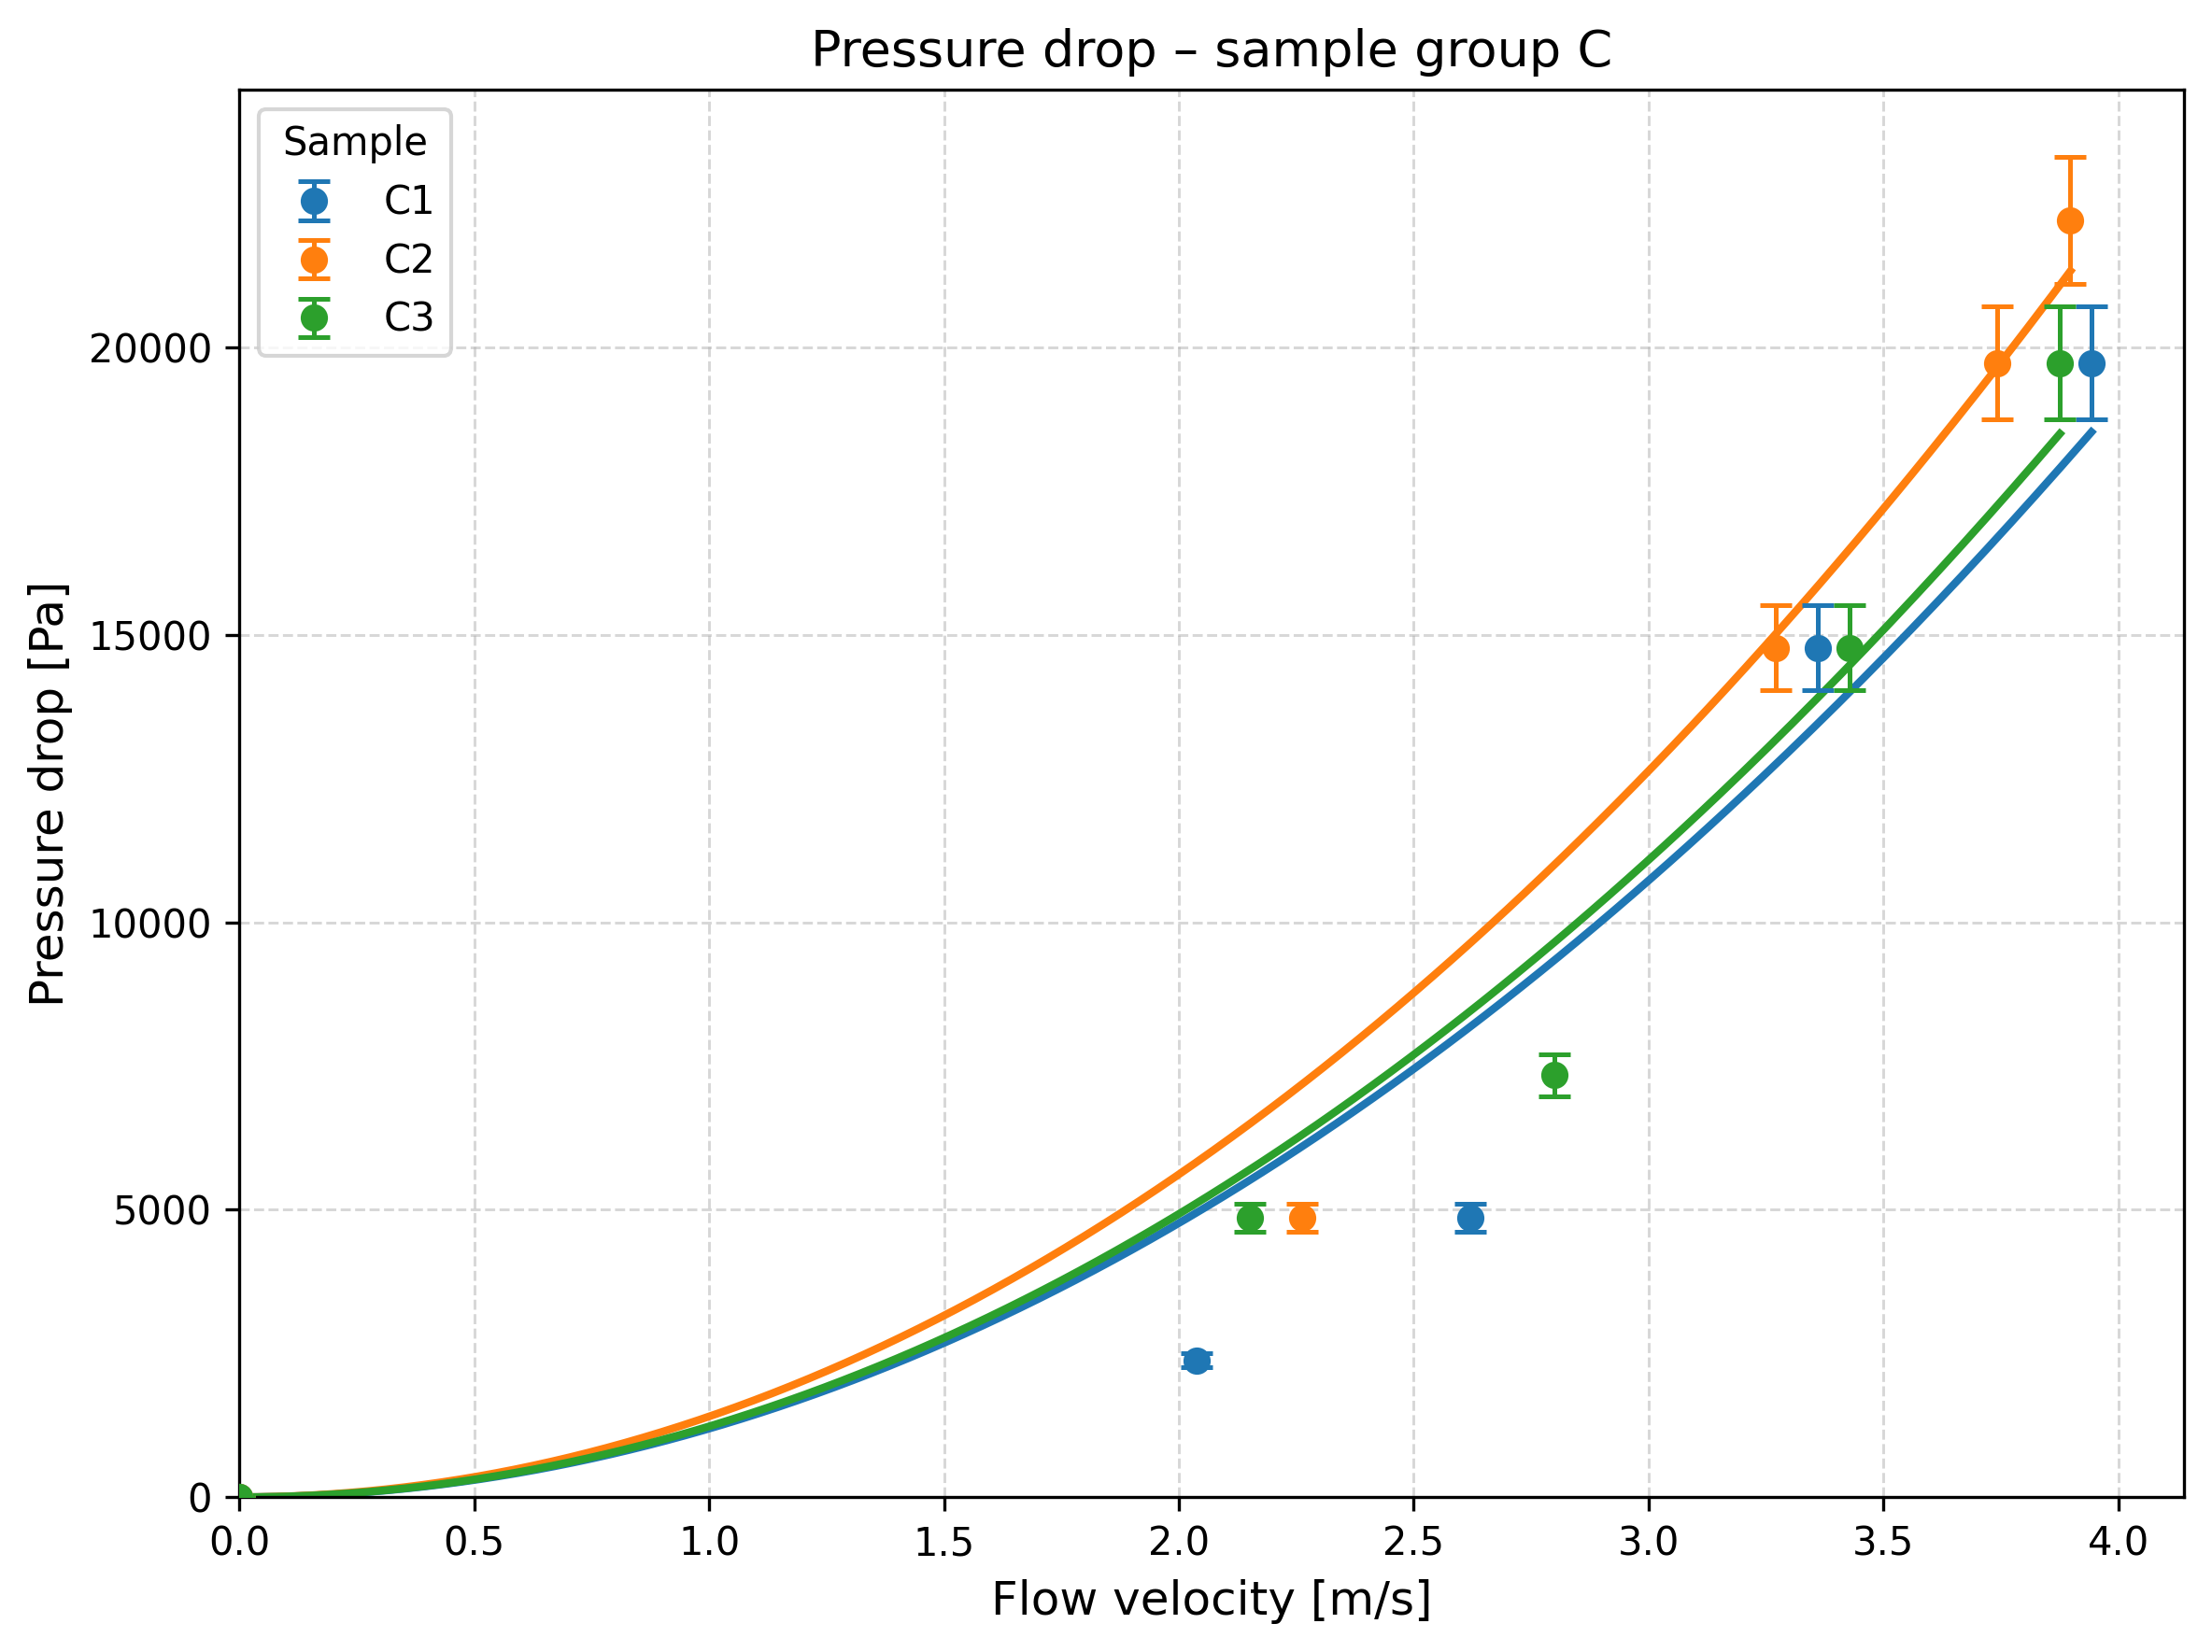
\includegraphics[width=10cm]{group_C_pressure_drop_velocity.png}
  \caption{Pressure drop across the porous zone for sample set C.}
\end{figure}

\begin{figure}[htbp]
  \centering
  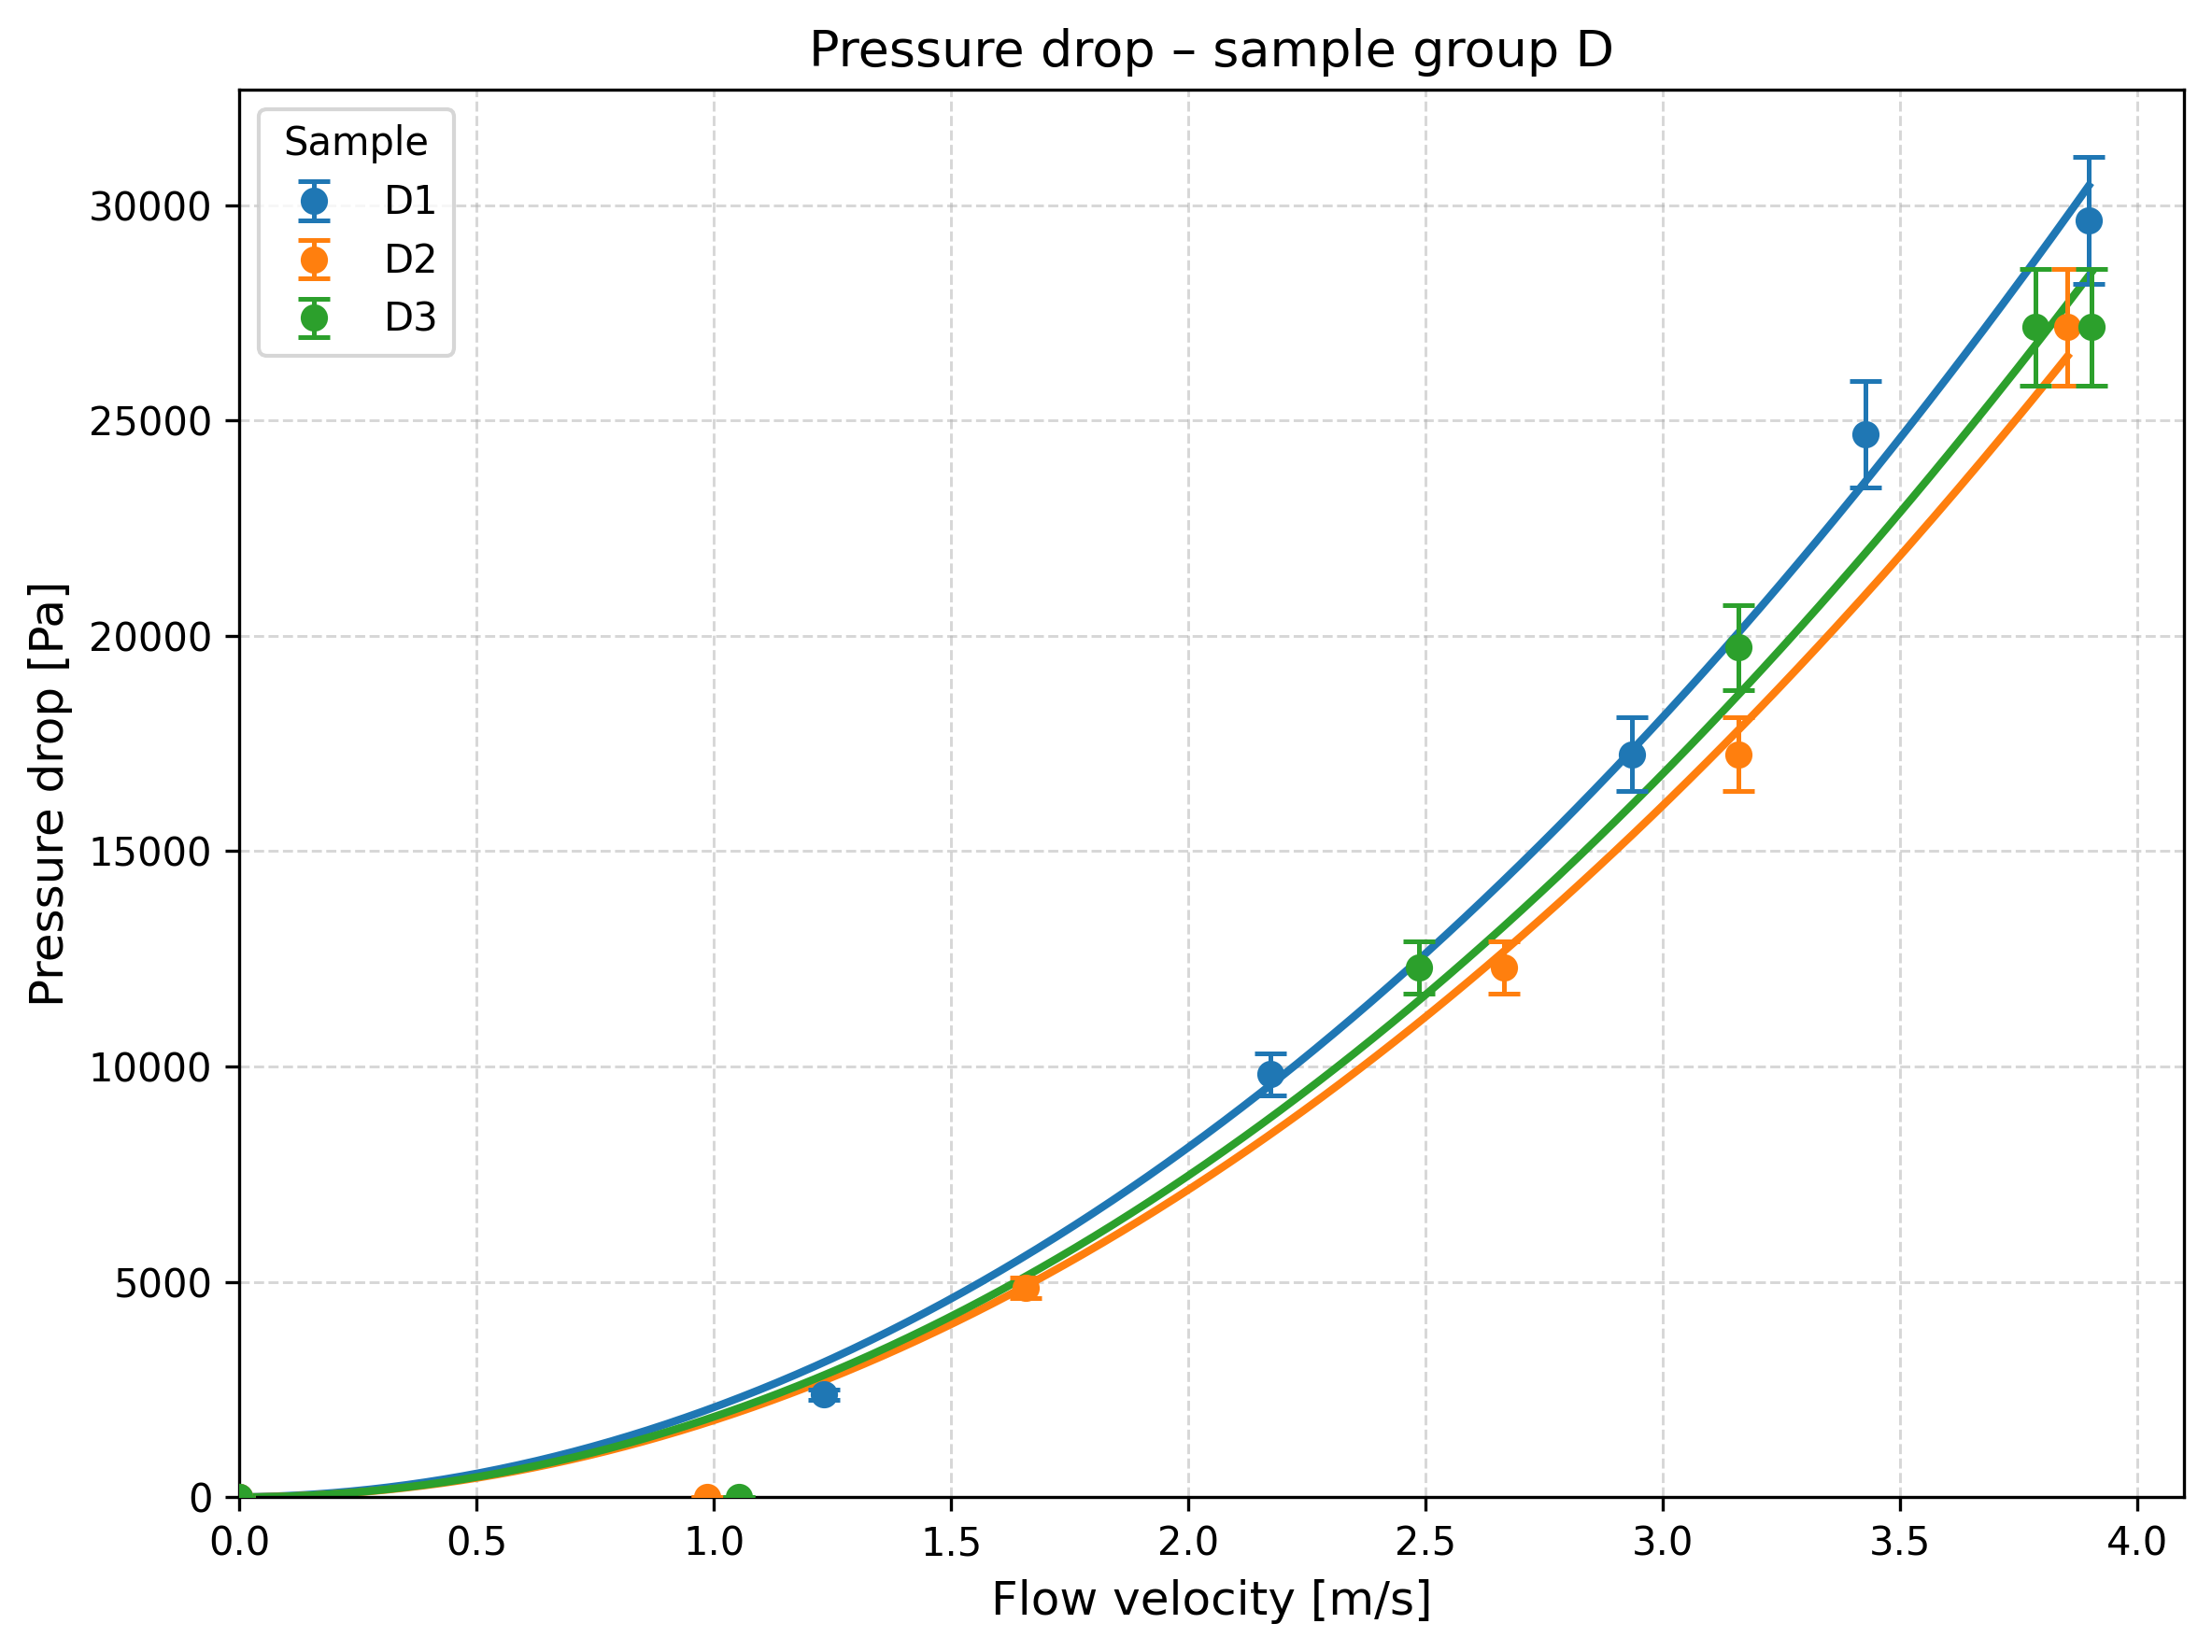
\includegraphics[width=10cm]{group_D_pressure_drop_velocity.png}
  \caption{Pressure drop across the porous zone for sample set D.}
\end{figure}

\begin{figure}[htbp]
  \centering
  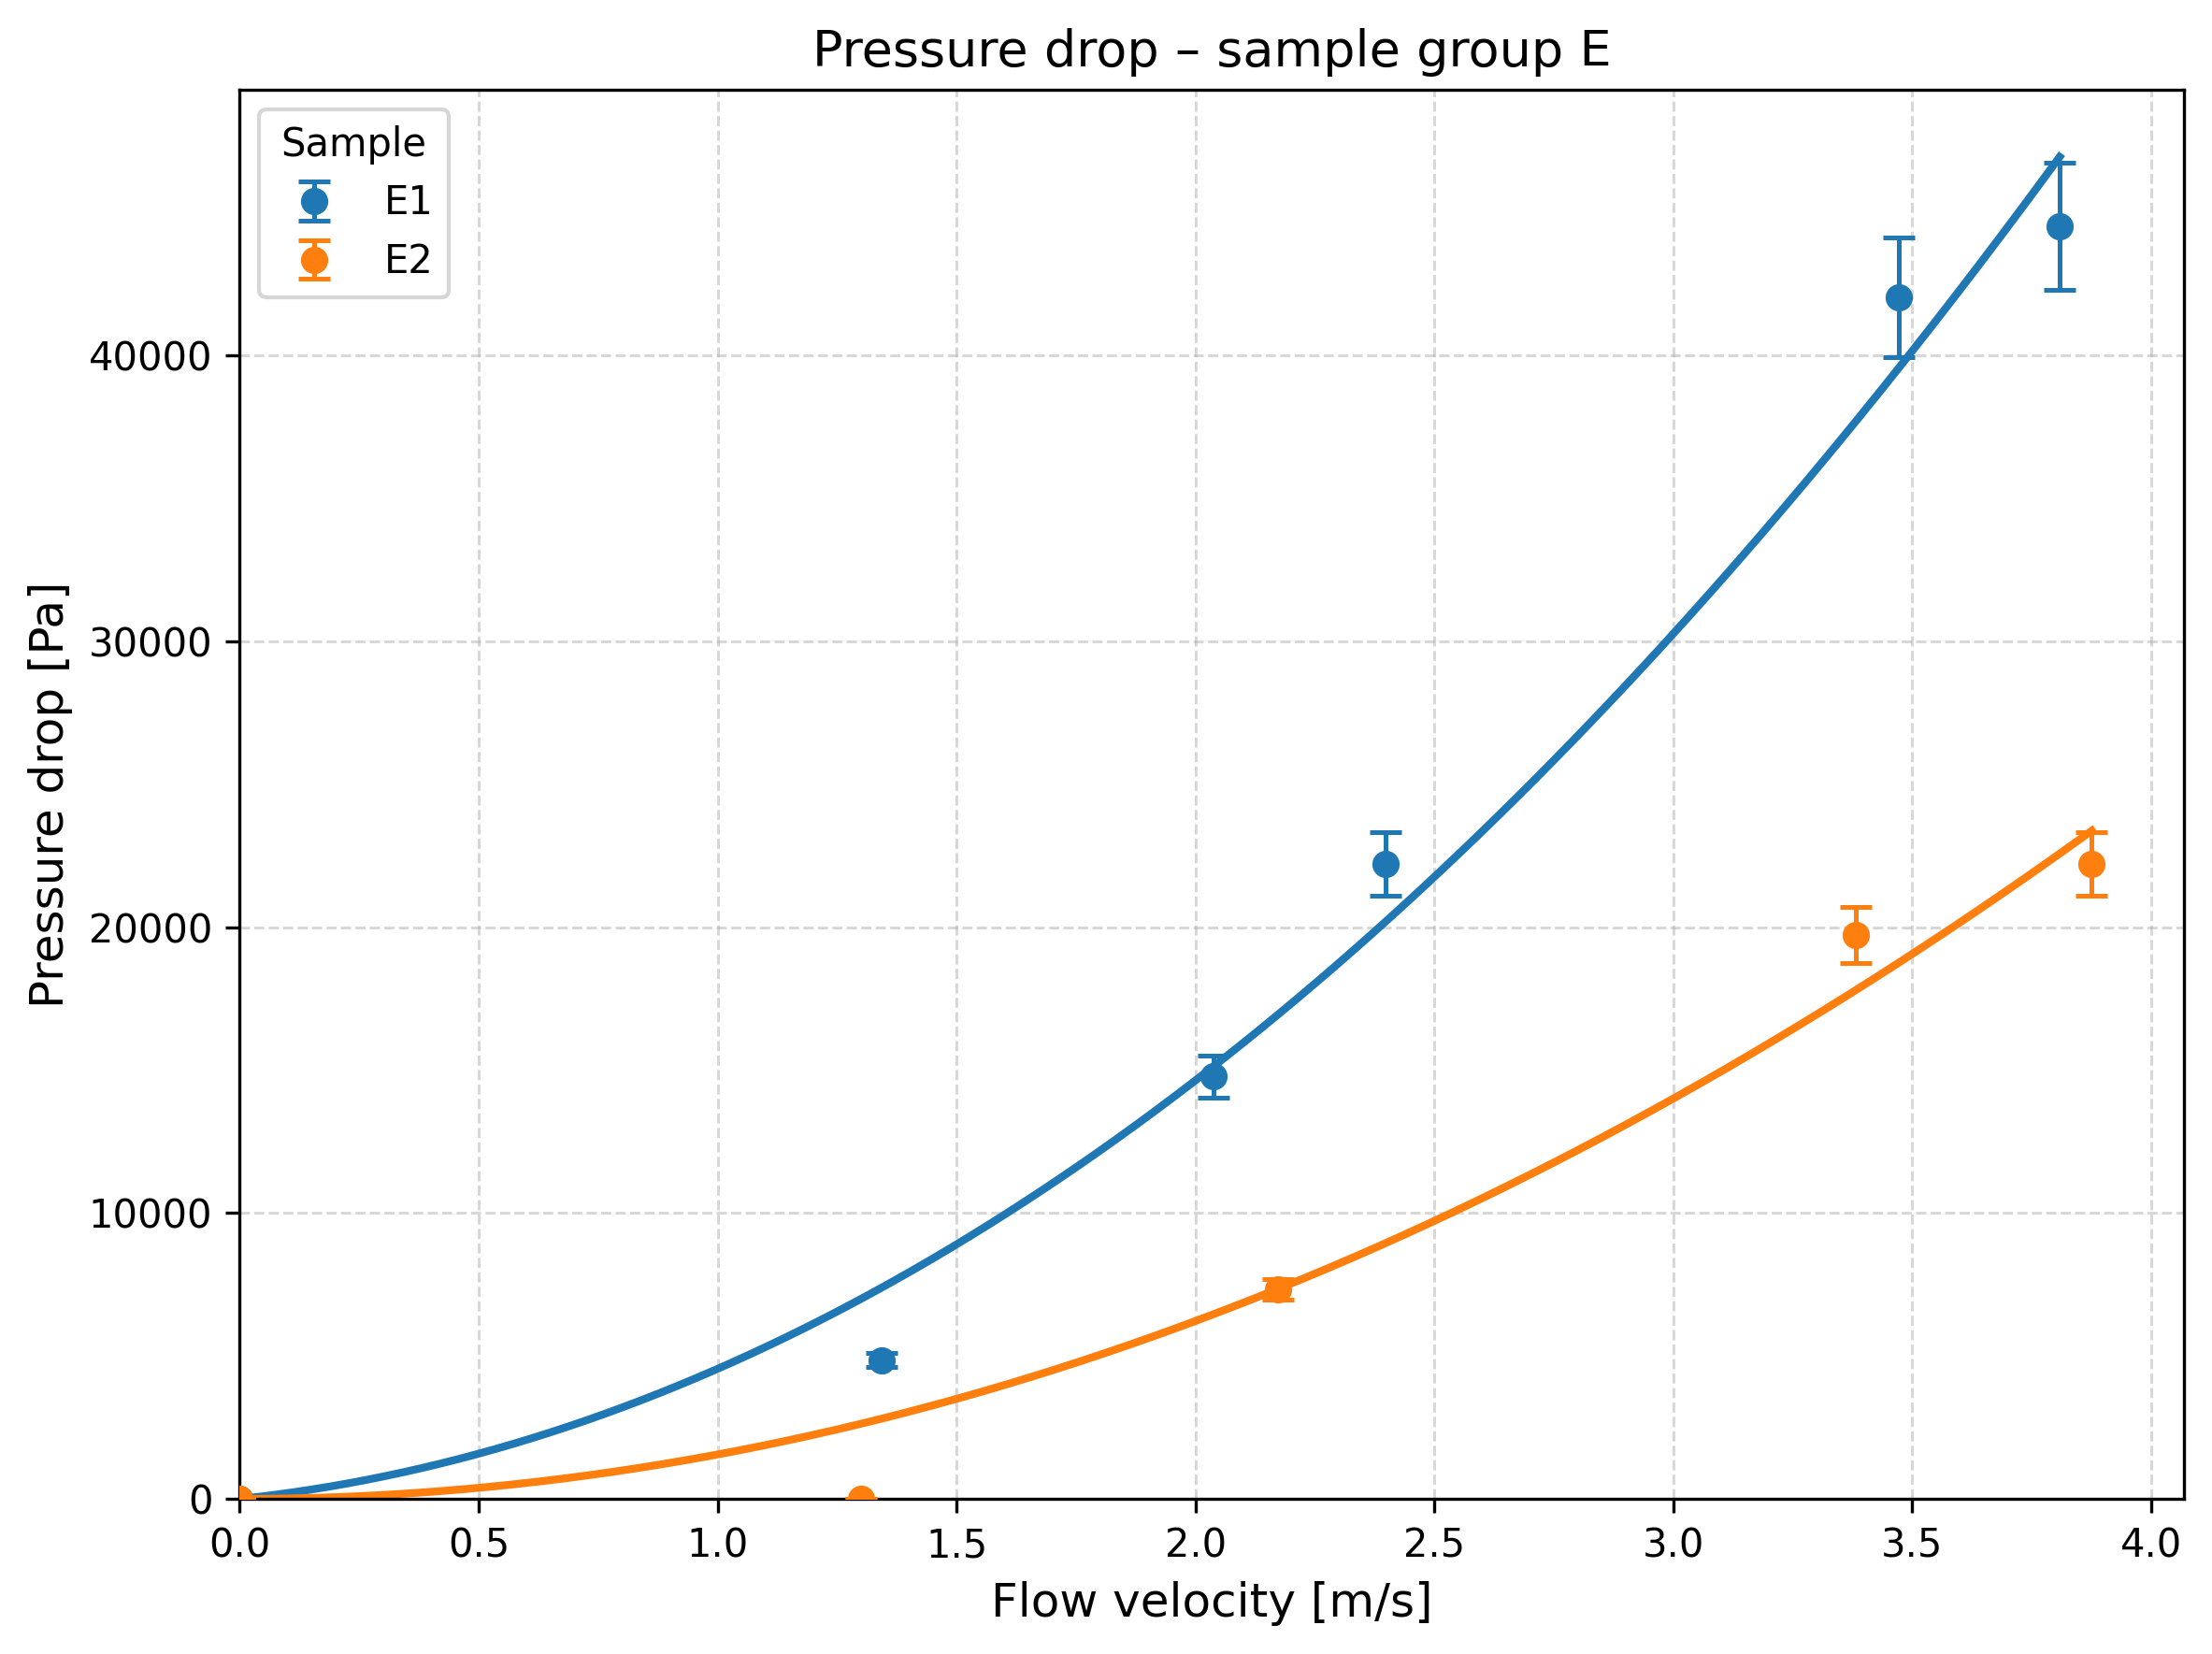
\includegraphics[width=10cm]{group_E_pressure_drop_velocity.png}
  \caption{Pressure drop across the porous zone for sample set E.}
\end{figure}

\clearpage

\end{document}